% Options for packages loaded elsewhere
\PassOptionsToPackage{unicode}{hyperref}
\PassOptionsToPackage{hyphens}{url}
%
\documentclass[
]{book}
\usepackage{amsmath,amssymb}
\usepackage{lmodern}
\usepackage{ifxetex,ifluatex}
\ifnum 0\ifxetex 1\fi\ifluatex 1\fi=0 % if pdftex
  \usepackage[T1]{fontenc}
  \usepackage[utf8]{inputenc}
  \usepackage{textcomp} % provide euro and other symbols
\else % if luatex or xetex
  \usepackage{unicode-math}
  \defaultfontfeatures{Scale=MatchLowercase}
  \defaultfontfeatures[\rmfamily]{Ligatures=TeX,Scale=1}
\fi
% Use upquote if available, for straight quotes in verbatim environments
\IfFileExists{upquote.sty}{\usepackage{upquote}}{}
\IfFileExists{microtype.sty}{% use microtype if available
  \usepackage[]{microtype}
  \UseMicrotypeSet[protrusion]{basicmath} % disable protrusion for tt fonts
}{}
\makeatletter
\@ifundefined{KOMAClassName}{% if non-KOMA class
  \IfFileExists{parskip.sty}{%
    \usepackage{parskip}
  }{% else
    \setlength{\parindent}{0pt}
    \setlength{\parskip}{6pt plus 2pt minus 1pt}}
}{% if KOMA class
  \KOMAoptions{parskip=half}}
\makeatother
\usepackage{xcolor}
\IfFileExists{xurl.sty}{\usepackage{xurl}}{} % add URL line breaks if available
\IfFileExists{bookmark.sty}{\usepackage{bookmark}}{\usepackage{hyperref}}
\hypersetup{
  pdftitle={R for Non-Programmers: A Guide for Social Scientists},
  pdfauthor={Daniel Dauber},
  hidelinks,
  pdfcreator={LaTeX via pandoc}}
\urlstyle{same} % disable monospaced font for URLs
\usepackage{color}
\usepackage{fancyvrb}
\newcommand{\VerbBar}{|}
\newcommand{\VERB}{\Verb[commandchars=\\\{\}]}
\DefineVerbatimEnvironment{Highlighting}{Verbatim}{commandchars=\\\{\}}
% Add ',fontsize=\small' for more characters per line
\usepackage{framed}
\definecolor{shadecolor}{RGB}{248,248,248}
\newenvironment{Shaded}{\begin{snugshade}}{\end{snugshade}}
\newcommand{\AlertTok}[1]{\textcolor[rgb]{0.94,0.16,0.16}{#1}}
\newcommand{\AnnotationTok}[1]{\textcolor[rgb]{0.56,0.35,0.01}{\textbf{\textit{#1}}}}
\newcommand{\AttributeTok}[1]{\textcolor[rgb]{0.77,0.63,0.00}{#1}}
\newcommand{\BaseNTok}[1]{\textcolor[rgb]{0.00,0.00,0.81}{#1}}
\newcommand{\BuiltInTok}[1]{#1}
\newcommand{\CharTok}[1]{\textcolor[rgb]{0.31,0.60,0.02}{#1}}
\newcommand{\CommentTok}[1]{\textcolor[rgb]{0.56,0.35,0.01}{\textit{#1}}}
\newcommand{\CommentVarTok}[1]{\textcolor[rgb]{0.56,0.35,0.01}{\textbf{\textit{#1}}}}
\newcommand{\ConstantTok}[1]{\textcolor[rgb]{0.00,0.00,0.00}{#1}}
\newcommand{\ControlFlowTok}[1]{\textcolor[rgb]{0.13,0.29,0.53}{\textbf{#1}}}
\newcommand{\DataTypeTok}[1]{\textcolor[rgb]{0.13,0.29,0.53}{#1}}
\newcommand{\DecValTok}[1]{\textcolor[rgb]{0.00,0.00,0.81}{#1}}
\newcommand{\DocumentationTok}[1]{\textcolor[rgb]{0.56,0.35,0.01}{\textbf{\textit{#1}}}}
\newcommand{\ErrorTok}[1]{\textcolor[rgb]{0.64,0.00,0.00}{\textbf{#1}}}
\newcommand{\ExtensionTok}[1]{#1}
\newcommand{\FloatTok}[1]{\textcolor[rgb]{0.00,0.00,0.81}{#1}}
\newcommand{\FunctionTok}[1]{\textcolor[rgb]{0.00,0.00,0.00}{#1}}
\newcommand{\ImportTok}[1]{#1}
\newcommand{\InformationTok}[1]{\textcolor[rgb]{0.56,0.35,0.01}{\textbf{\textit{#1}}}}
\newcommand{\KeywordTok}[1]{\textcolor[rgb]{0.13,0.29,0.53}{\textbf{#1}}}
\newcommand{\NormalTok}[1]{#1}
\newcommand{\OperatorTok}[1]{\textcolor[rgb]{0.81,0.36,0.00}{\textbf{#1}}}
\newcommand{\OtherTok}[1]{\textcolor[rgb]{0.56,0.35,0.01}{#1}}
\newcommand{\PreprocessorTok}[1]{\textcolor[rgb]{0.56,0.35,0.01}{\textit{#1}}}
\newcommand{\RegionMarkerTok}[1]{#1}
\newcommand{\SpecialCharTok}[1]{\textcolor[rgb]{0.00,0.00,0.00}{#1}}
\newcommand{\SpecialStringTok}[1]{\textcolor[rgb]{0.31,0.60,0.02}{#1}}
\newcommand{\StringTok}[1]{\textcolor[rgb]{0.31,0.60,0.02}{#1}}
\newcommand{\VariableTok}[1]{\textcolor[rgb]{0.00,0.00,0.00}{#1}}
\newcommand{\VerbatimStringTok}[1]{\textcolor[rgb]{0.31,0.60,0.02}{#1}}
\newcommand{\WarningTok}[1]{\textcolor[rgb]{0.56,0.35,0.01}{\textbf{\textit{#1}}}}
\usepackage{longtable,booktabs,array}
\usepackage{calc} % for calculating minipage widths
% Correct order of tables after \paragraph or \subparagraph
\usepackage{etoolbox}
\makeatletter
\patchcmd\longtable{\par}{\if@noskipsec\mbox{}\fi\par}{}{}
\makeatother
% Allow footnotes in longtable head/foot
\IfFileExists{footnotehyper.sty}{\usepackage{footnotehyper}}{\usepackage{footnote}}
\makesavenoteenv{longtable}
\usepackage{graphicx}
\makeatletter
\def\maxwidth{\ifdim\Gin@nat@width>\linewidth\linewidth\else\Gin@nat@width\fi}
\def\maxheight{\ifdim\Gin@nat@height>\textheight\textheight\else\Gin@nat@height\fi}
\makeatother
% Scale images if necessary, so that they will not overflow the page
% margins by default, and it is still possible to overwrite the defaults
% using explicit options in \includegraphics[width, height, ...]{}
\setkeys{Gin}{width=\maxwidth,height=\maxheight,keepaspectratio}
% Set default figure placement to htbp
\makeatletter
\def\fps@figure{htbp}
\makeatother
\setlength{\emergencystretch}{3em} % prevent overfull lines
\providecommand{\tightlist}{%
  \setlength{\itemsep}{0pt}\setlength{\parskip}{0pt}}
\setcounter{secnumdepth}{5}
\usepackage{booktabs}
\ifluatex
  \usepackage{selnolig}  % disable illegal ligatures
\fi
\usepackage[]{natbib}
\bibliographystyle{apalike}

\title{R for Non-Programmers: A Guide for Social Scientists}
\author{Daniel Dauber}
\date{2021-09-16}

\begin{document}
\maketitle

{
\setcounter{tocdepth}{1}
\tableofcontents
}
\hypertarget{welcome}{%
\chapter*{Welcome 👋}\label{welcome}}
\addcontentsline{toc}{chapter}{Welcome 👋}


\includegraphics{images/chapter_00_img/r_for_non_programmers_logo.png}

Welcome to \emph{R for Non-Programmers: A guide for Social Scientists}. This book is intended to be of help to everyone who wishes to enter the world of R Programming, but not necessarily for the purpose to become a programmer. Instead, this book intends to convey key concepts in data analysis, especially quantitative research.

{[}Add more{]}

\hypertarget{acknowledgments}{%
\chapter*{Acknowledgments 🙏}\label{acknowledgments}}
\addcontentsline{toc}{chapter}{Acknowledgments 🙏}

Special thanks are due to my wife, who supported me in so many ways to get this book completed. Also, I would like to thank my son, who patiently watched me sitting at the computer type this book up.

\hypertarget{readme-before-you-get-started}{%
\chapter{\texorpdfstring{\texttt{Readme.} Before you get started}{Readme. Before you get started}}\label{readme-before-you-get-started}}

\hypertarget{a-starting-point-and-reference-book}{%
\section{A starting point and reference book}\label{a-starting-point-and-reference-book}}

\texttt{to\ be\ added}

\hypertarget{download-the-companion-r-package}{%
\section{Download the companion R package}\label{download-the-companion-r-package}}

\texttt{to\ be\ added}

\begin{itemize}
\item
  Explain where to download
\item
  Explain how examples are shown in this book (code in the first grey box, console results in the second grey box
\end{itemize}

\hypertarget{a-tidyverse-approach-with-some-basic-r}{%
\section{A `tidyverse' approach with some basic R}\label{a-tidyverse-approach-with-some-basic-r}}

\texttt{to\ be\ added}

\hypertarget{why-learn-a-programming-language-as-a-non-programmer}{%
\chapter{Why learn a programming language as a non-programmer?}\label{why-learn-a-programming-language-as-a-non-programmer}}

\emph{`R'}, it is not just a letter you learn in primary school, but a powerful programming language. While it is used for a lot of quantitative data analysis, it has grown over the years to become a powerful tool that excels (\#no-pun-intended) in handling data and performing customised computations with quantitative and qualitative data.

\emph{R}~is now one of my core tools to perform various types of analysis because I can use it in many different ways, for example,

\begin{itemize}
\tightlist
\item
  statistical analysis,
\item
  corpus analysis,
\item
  development of online dashboards to dynamically generate interactive data visualisations,
\item
  connection to social media APIs for data collection,
\item
  Creation of reporting systems to provide individualised feedback to research participants,
\item
  Drafting and writing research articles, etc.
\end{itemize}

\begin{quote}
\emph{Learning R is like learning a foreign language. If you like learning languages, then `R' is just another one.}
\end{quote}

While \emph{R} has become a comprehensive tool for data scientists, it has yet to find its way into the mainstream field of Social Sciences. Why? Well, learning programming languages is not necessarily something that feels comfortable to everyone. It is not like Microsoft Word, where you can open the software and explore it through trial and error. Learning a programming language is like learning a foreign language: You have to learn vocabulary, grammar and syntax. Similar to learning a new language, programming languages also have steep learning curves and require quite some commitment.

For this reason, most people do not even dare to learn it because it is time-consuming and often not considered a \emph{`core method'} in Social Sciences disciplines. Apart from that, tools like SPSS have very intuitive interfaces, which seem much easier to use (or not?). However, the feeling of having \emph{`mastered'} \emph{R} (although one might never be able to claim this) can be extremely rewarding.

I guess this introduction was not necessarily helpful in convincing you to learn any programming language. However, despite those initial hurdles, there are a series of advantages to consider. Below I list some good reasons to learn a programming language as they pertain to my own experiences.

\hypertarget{learning-new-tools-to-analyse-your-data-is-always-essential}{%
\section{Learning new tools to analyse your data is always essential}\label{learning-new-tools-to-analyse-your-data-is-always-essential}}

Theories change over time, and new insights into certain social phenomena are published every day. Thus, your knowledge might get outdated quite quickly. This is not so much the case for research methods knowledge. Typically, analytical techniques remain over many years. We still use the mean, mode, quartiles, standard deviation, etc., to describe our quantitative data. Still, there are always new computational methods that help us to crunch the numbers even more. \emph{R} is a tool that allows you to venture into new analytical territory because it is open source. Thousands of developers provide cutting-edge research methods free of charge for you to try with your data. You can find them on platforms like \href{https://github.com}{GitHub}. \emph{R} is like a giant supermarket, where all products are available for free. However, to read the labels on the product packaging and understand what they are, you have to learn the language used in this supermarket.

\hypertarget{programming-languages-enhance-your-conceptual-thinking}{%
\section{Programming languages enhance your conceptual thinking}\label{programming-languages-enhance-your-conceptual-thinking}}

While I have no empirical evidence for this, I am very certain it is true. While I would argue that my conceptual thinking is quite good, I would not necessarily say that I was born with it. Programming languages are very logical. Any error in your code will make you fail to execute it properly. Sometimes you face challenges in creating the correct code to solve a problem. Through creative abstract thinking (I should copyright this term), you start to approach your problems differently, whether it is a coding problem or a problem in any other context. For example, I know many students enjoy the process of qualitative coding. However, they often struggle to detach their insights from the actual data and synthesise ideas on an abstract and more generic level. Qualitative researchers might refer to this as challenges in '\emph{second-order deconstruction of meaning'}. This process of abstraction is a skill that needs to be honed, nurtured and practised. From my experience, programming languages are one way to achieve this, but they might not be recognised for this just yet.

\hypertarget{programming-languages-allow-you-to-look-at-your-data-from-a-different-angle}{%
\section{Programming languages allow you to look at your data from a different angle}\label{programming-languages-allow-you-to-look-at-your-data-from-a-different-angle}}

There are certainly commonly known and well-established techniques regarding how you should analyse your data rigorously. However, it can be quite some fun to try techniques outside your disciplines. This does not only apply to programming languages, of course. Sometimes, learning about a new research method enables you to look at your current tools in very different ways too. One of the biggest challenges for any researcher is to reflect on your work. Learning new and maybe even \emph{`strange'} tools can help with this. Admittedly, sometimes you might find out that some new tools are also a dead-end. Still, you might have learned something valuable through the process of engaging with your data differently. So shake off the rust of your analytical routine and blow some fresh air into your research methods.

\hypertarget{learning-any-programming-language-will-help-you-learn-other-programming-languages.}{%
\section{Learning any programming language will help you learn other programming languages.}\label{learning-any-programming-language-will-help-you-learn-other-programming-languages.}}

Once you understand the logic of one language, you will find it relatively easy to understand new programming languages. Of course, if you wanted to, you could become the next '\emph{Neo'} (from \href{https://www.imdb.com/title/tt0133093/?ref_=ext_shr_lnk}{`The Matrix')} and change the reality of your research forever. On a more serious note, though, if you know any programming language already, learning R will be easier because you have accrued some basic understanding of these particular types of languages.

Having considered everything of the above, do you feel ready for your next foreign language?

\hypertarget{setting-up-r-and-rstudio}{%
\chapter{Setting up R and RStudio}\label{setting-up-r-and-rstudio}}

Every journey starts with gathering the right equipment. This intellectual journey is not much different. The first step that every '\emph{R} novice has to face is to set everything up to get started. There are essentially two strategies:

\begin{itemize}
\tightlist
\item
  Install \href{https://www.r-project.org}{\emph{R}}and \href{https://www.rstudio.com}{RStudio}
\end{itemize}

or

\begin{itemize}
\tightlist
\item
  Run RStudio in a browser via \href{https://rstudio.cloud}{RStudio Cloud}
\end{itemize}

While installing~\emph{R}~and Studio requires more time and effort, I strongly recommend it, especially if you want to work offline or make good use of your computer's CPU. However, if you are not sure yet whether you enjoy learning~\emph{R}, you might wish to look at RStudio Cloud first. Either way, you can follow the examples of this book no matter which choice you make.

\hypertarget{installing-r}{%
\section{Installing R}\label{installing-r}}

The core module of our programming is R itself, and since it is an open-source project, it is available for free on Windows, Mac and Linux computers. Here is what you need to do to install it properly on your computer of choice:

\begin{enumerate}
\def\labelenumi{\arabic{enumi}.}
\item
  Go to \href{https://www.r-project.org\%5D(https://www.r-project.org)}{www.r-project.org}

  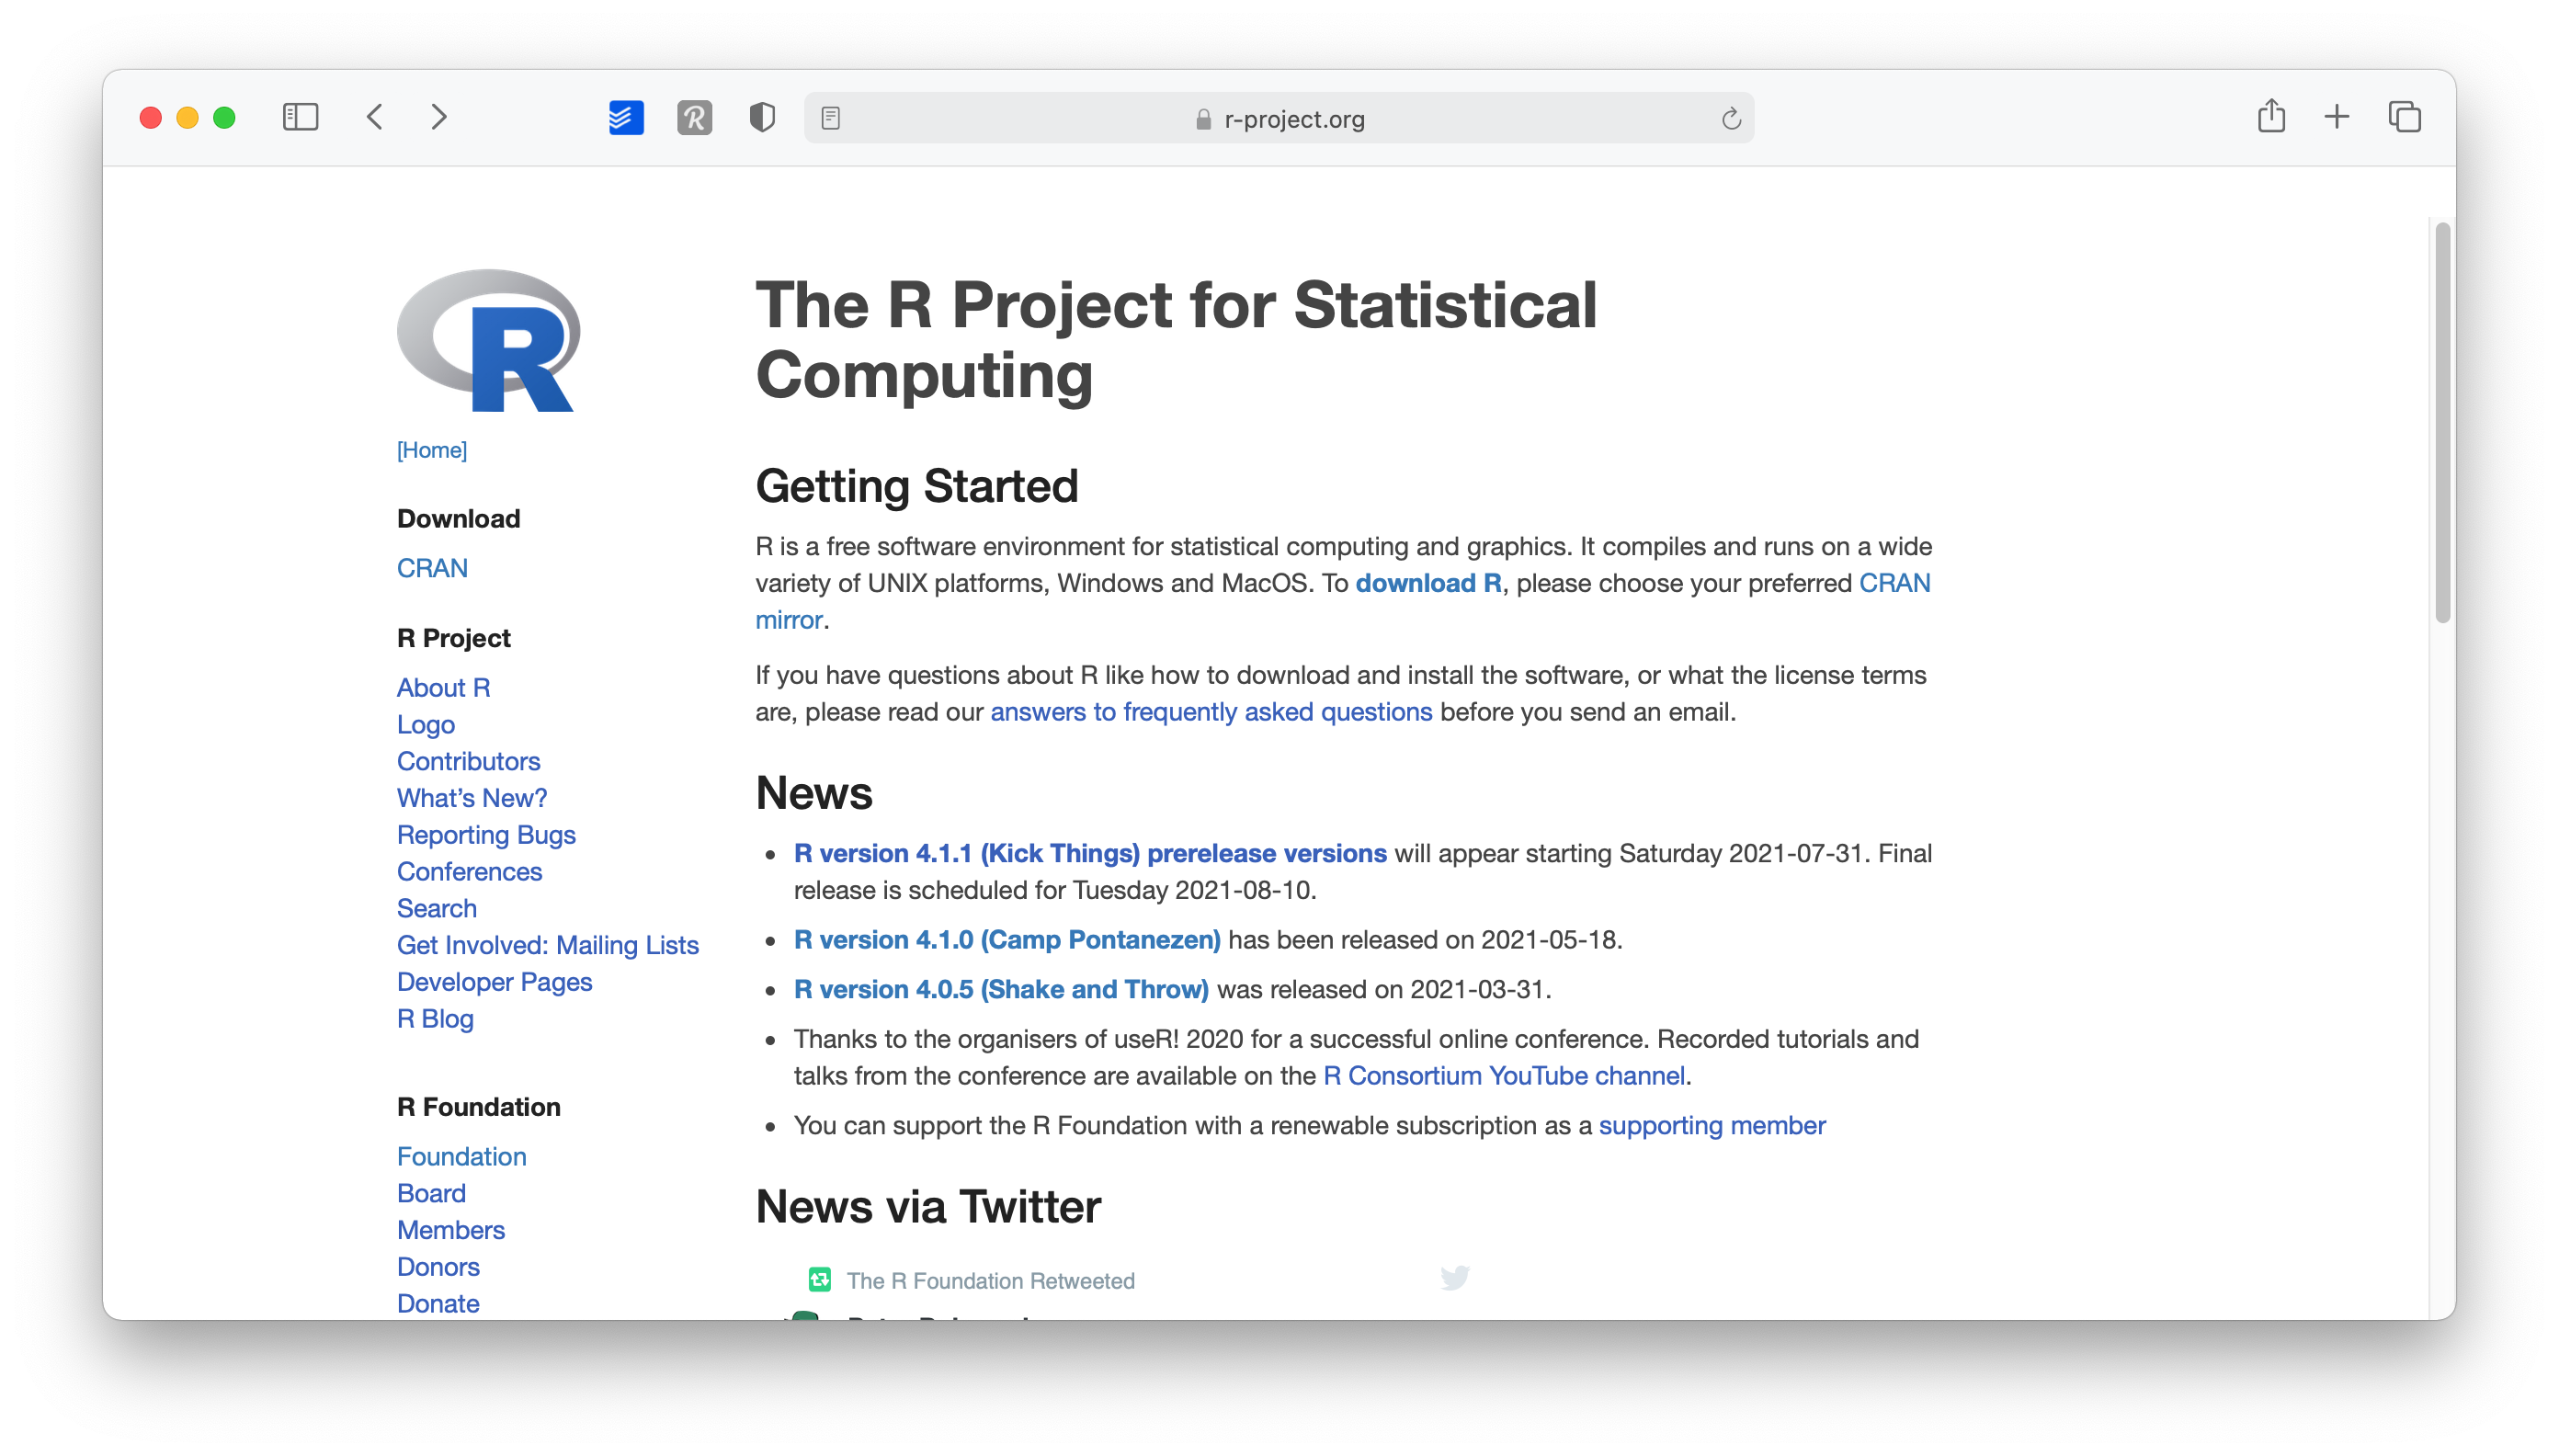
\includegraphics{images/chapter_03_img/r_project/00_r_project_page.png}
\item
  Click on \texttt{CRAN} where it says download.
\item
  Choose a server in your country (all of them work, but downloads will perform quicker).

  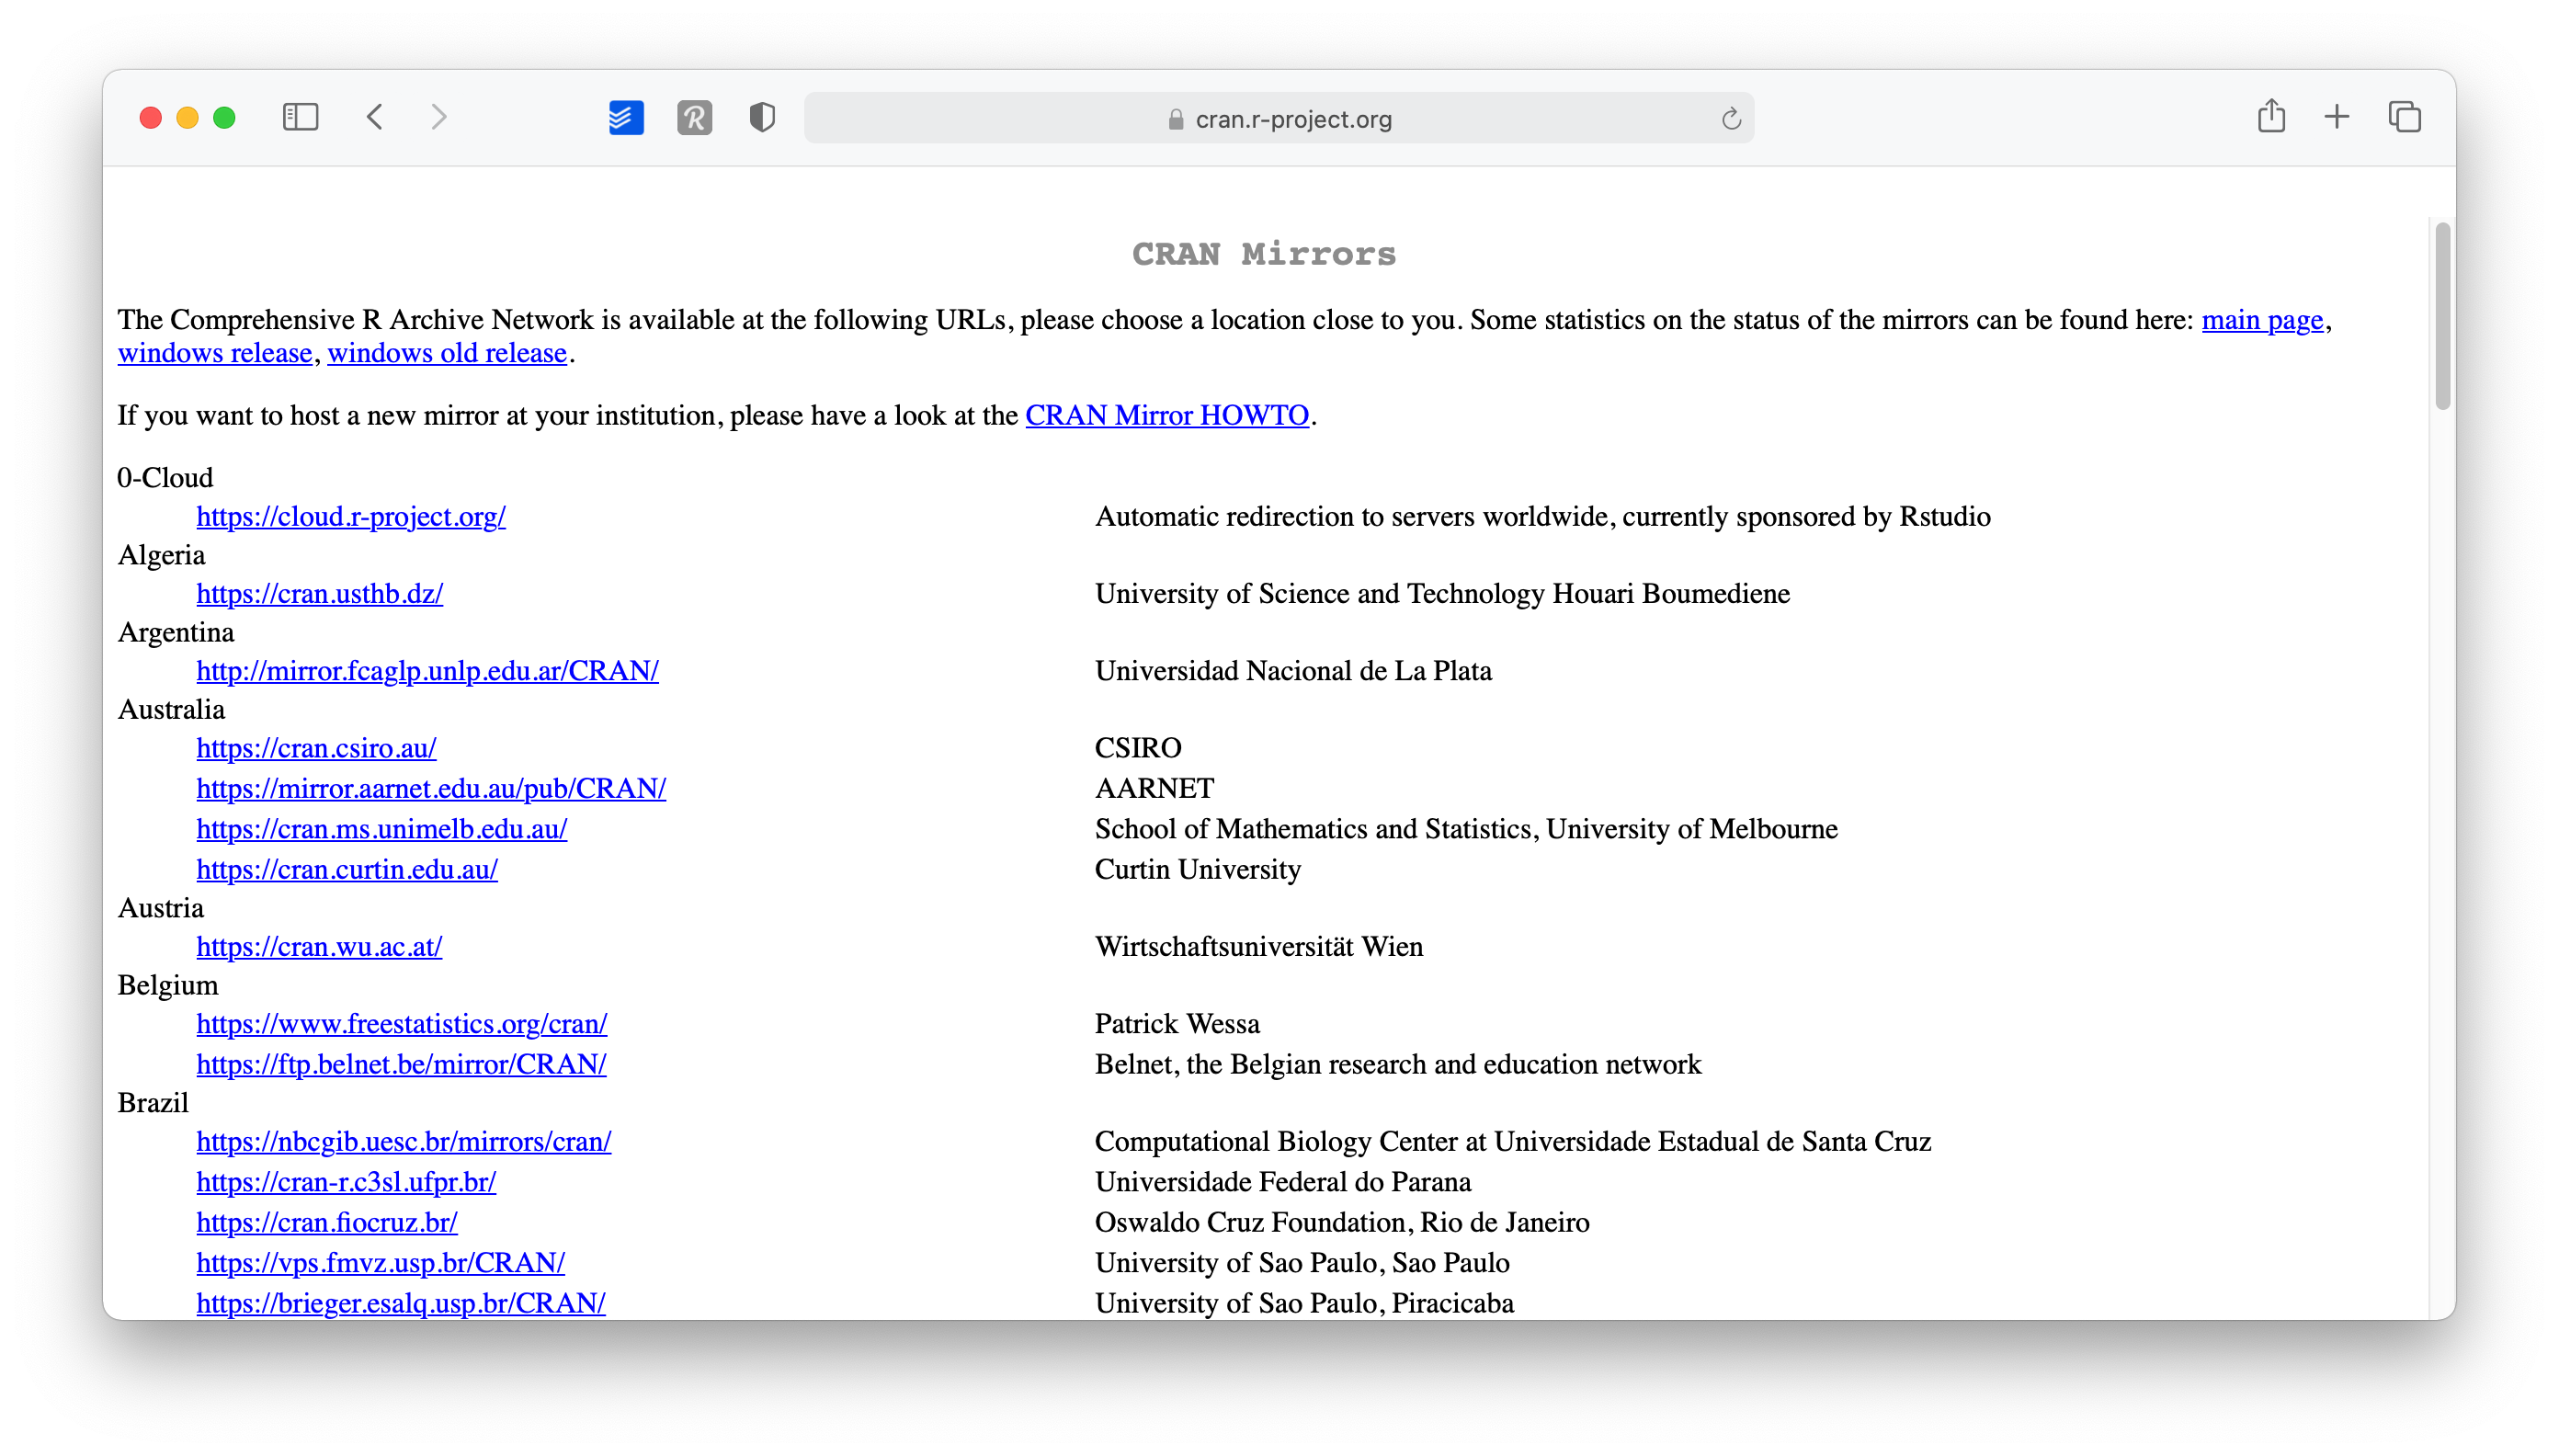
\includegraphics{images/chapter_03_img/r_project/01_r_project_cran_mirror.png}
\item
  Select the operating system for your computer.

  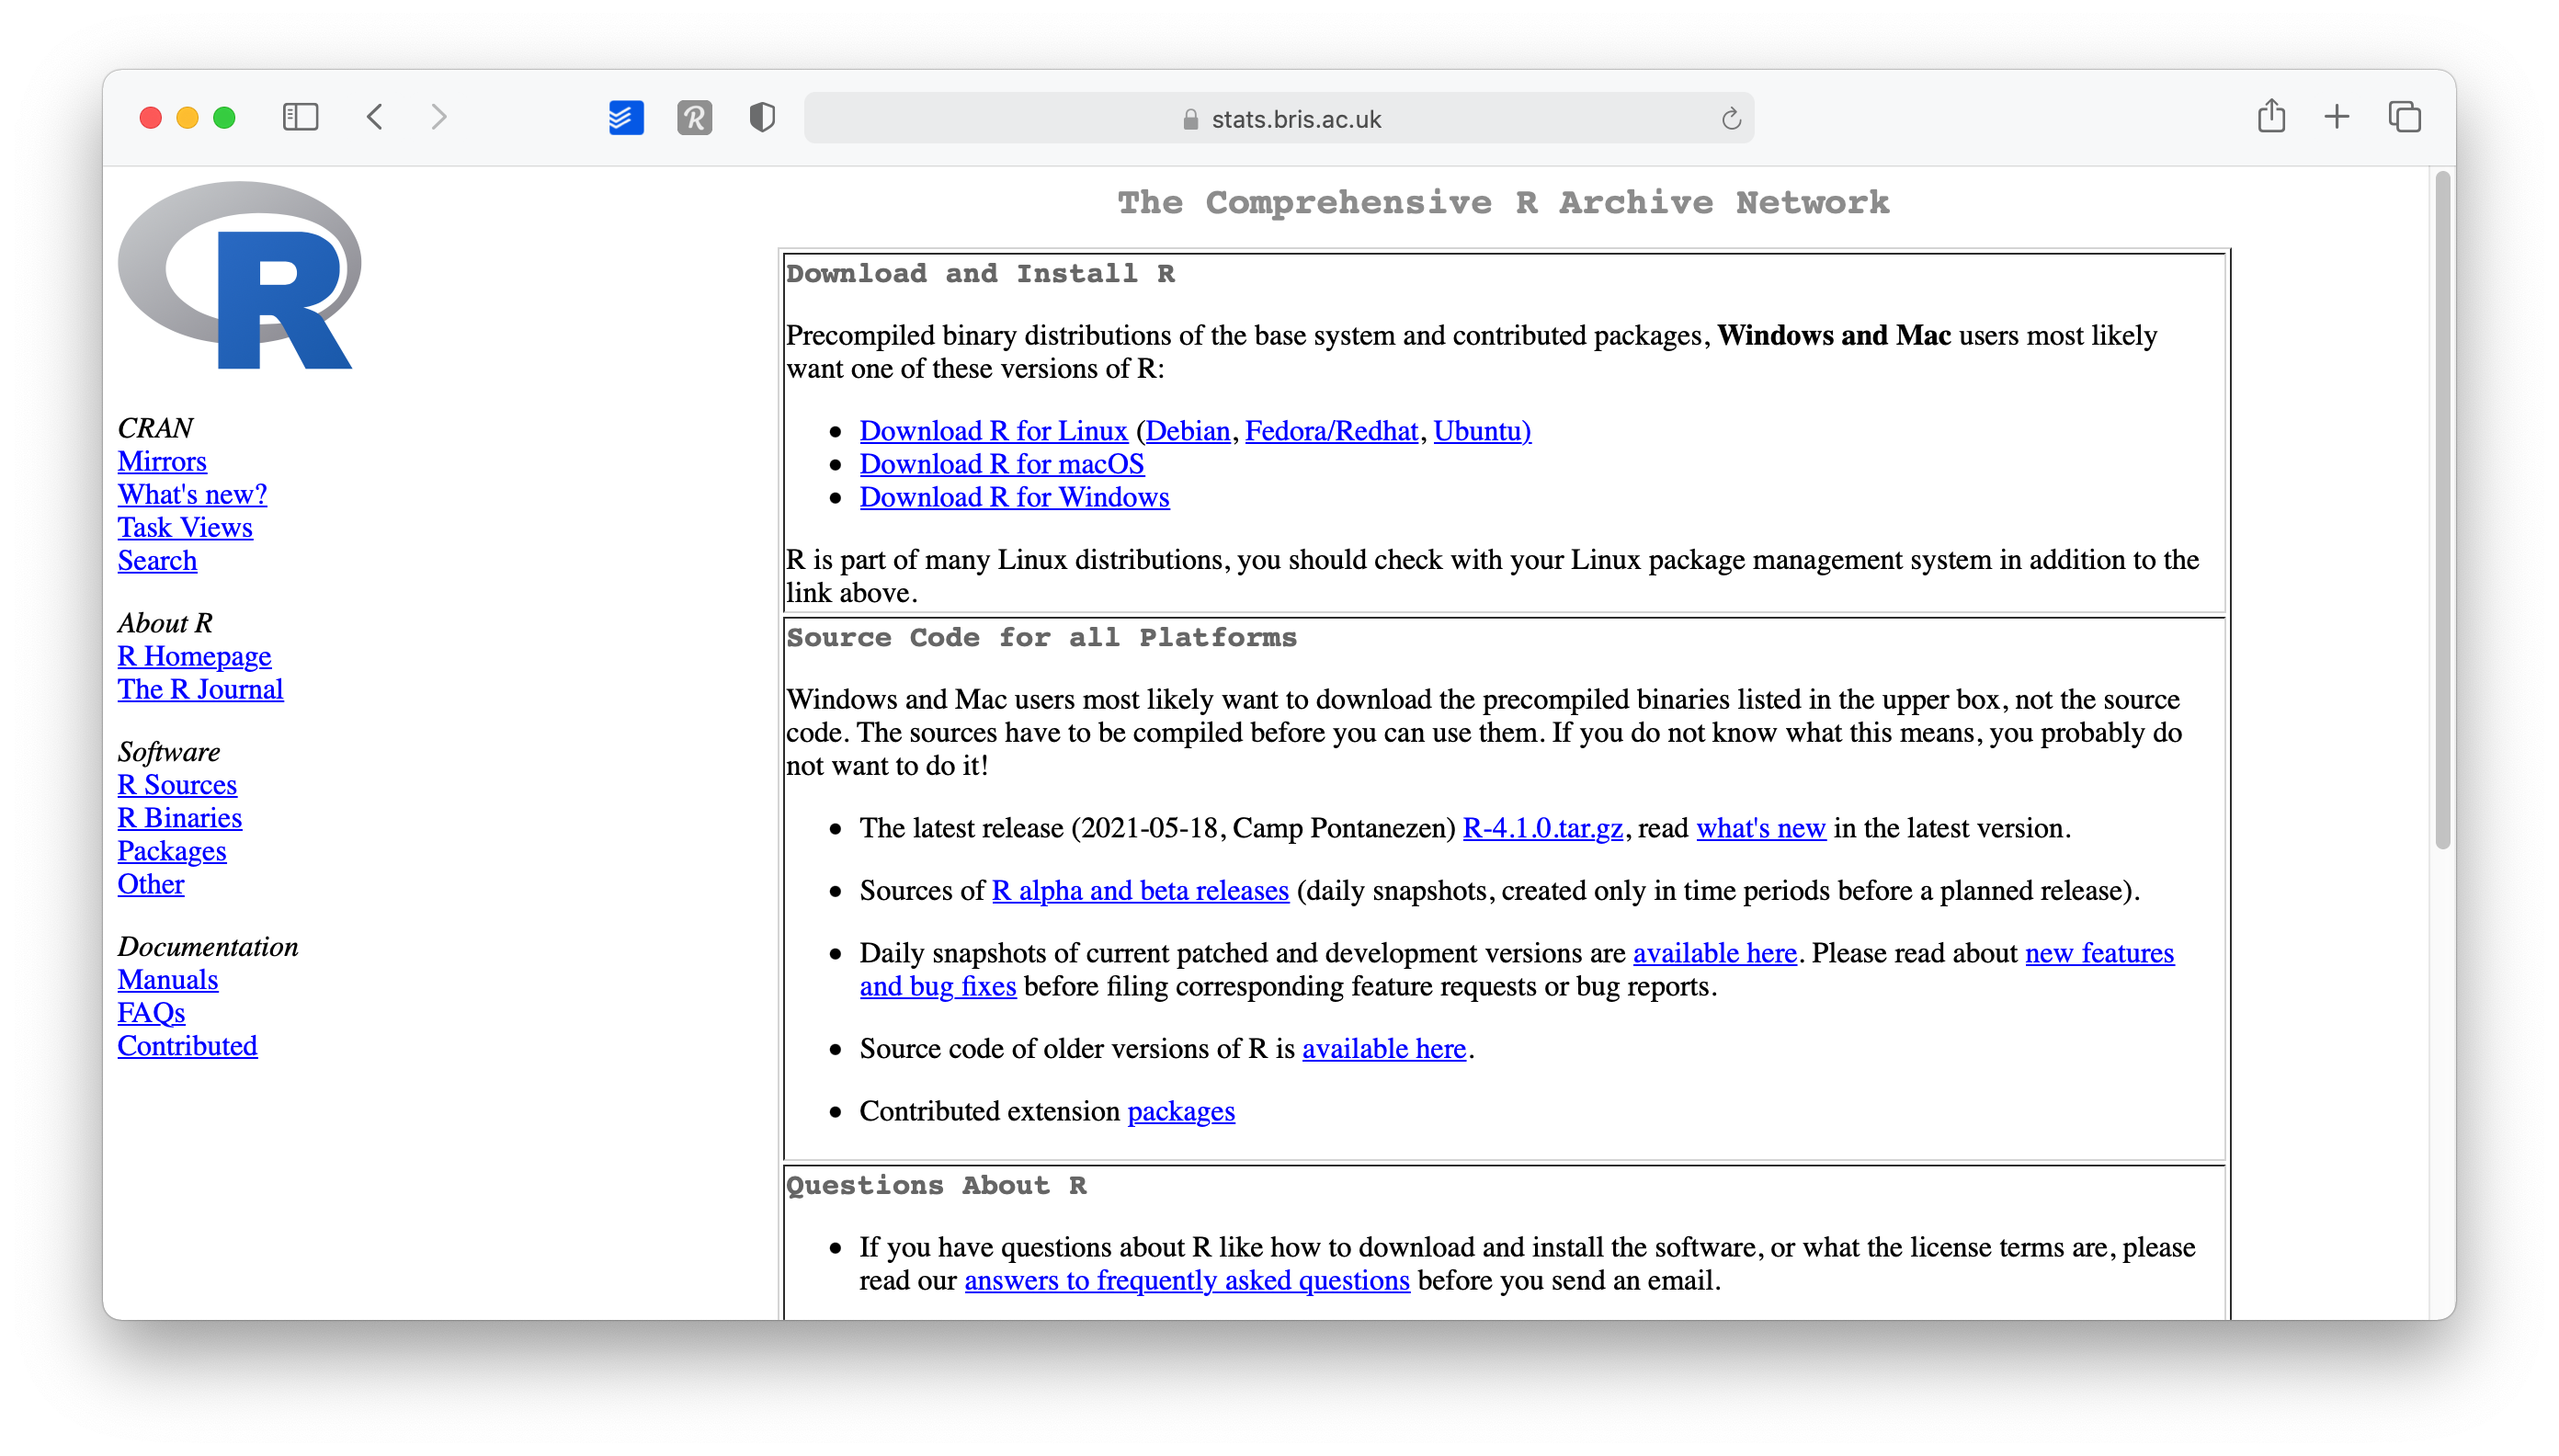
\includegraphics{images/chapter_03_img/r_project/02_r_project_os_choice.png}
\item
  Select the version you want to install (I recommend the latest version)

  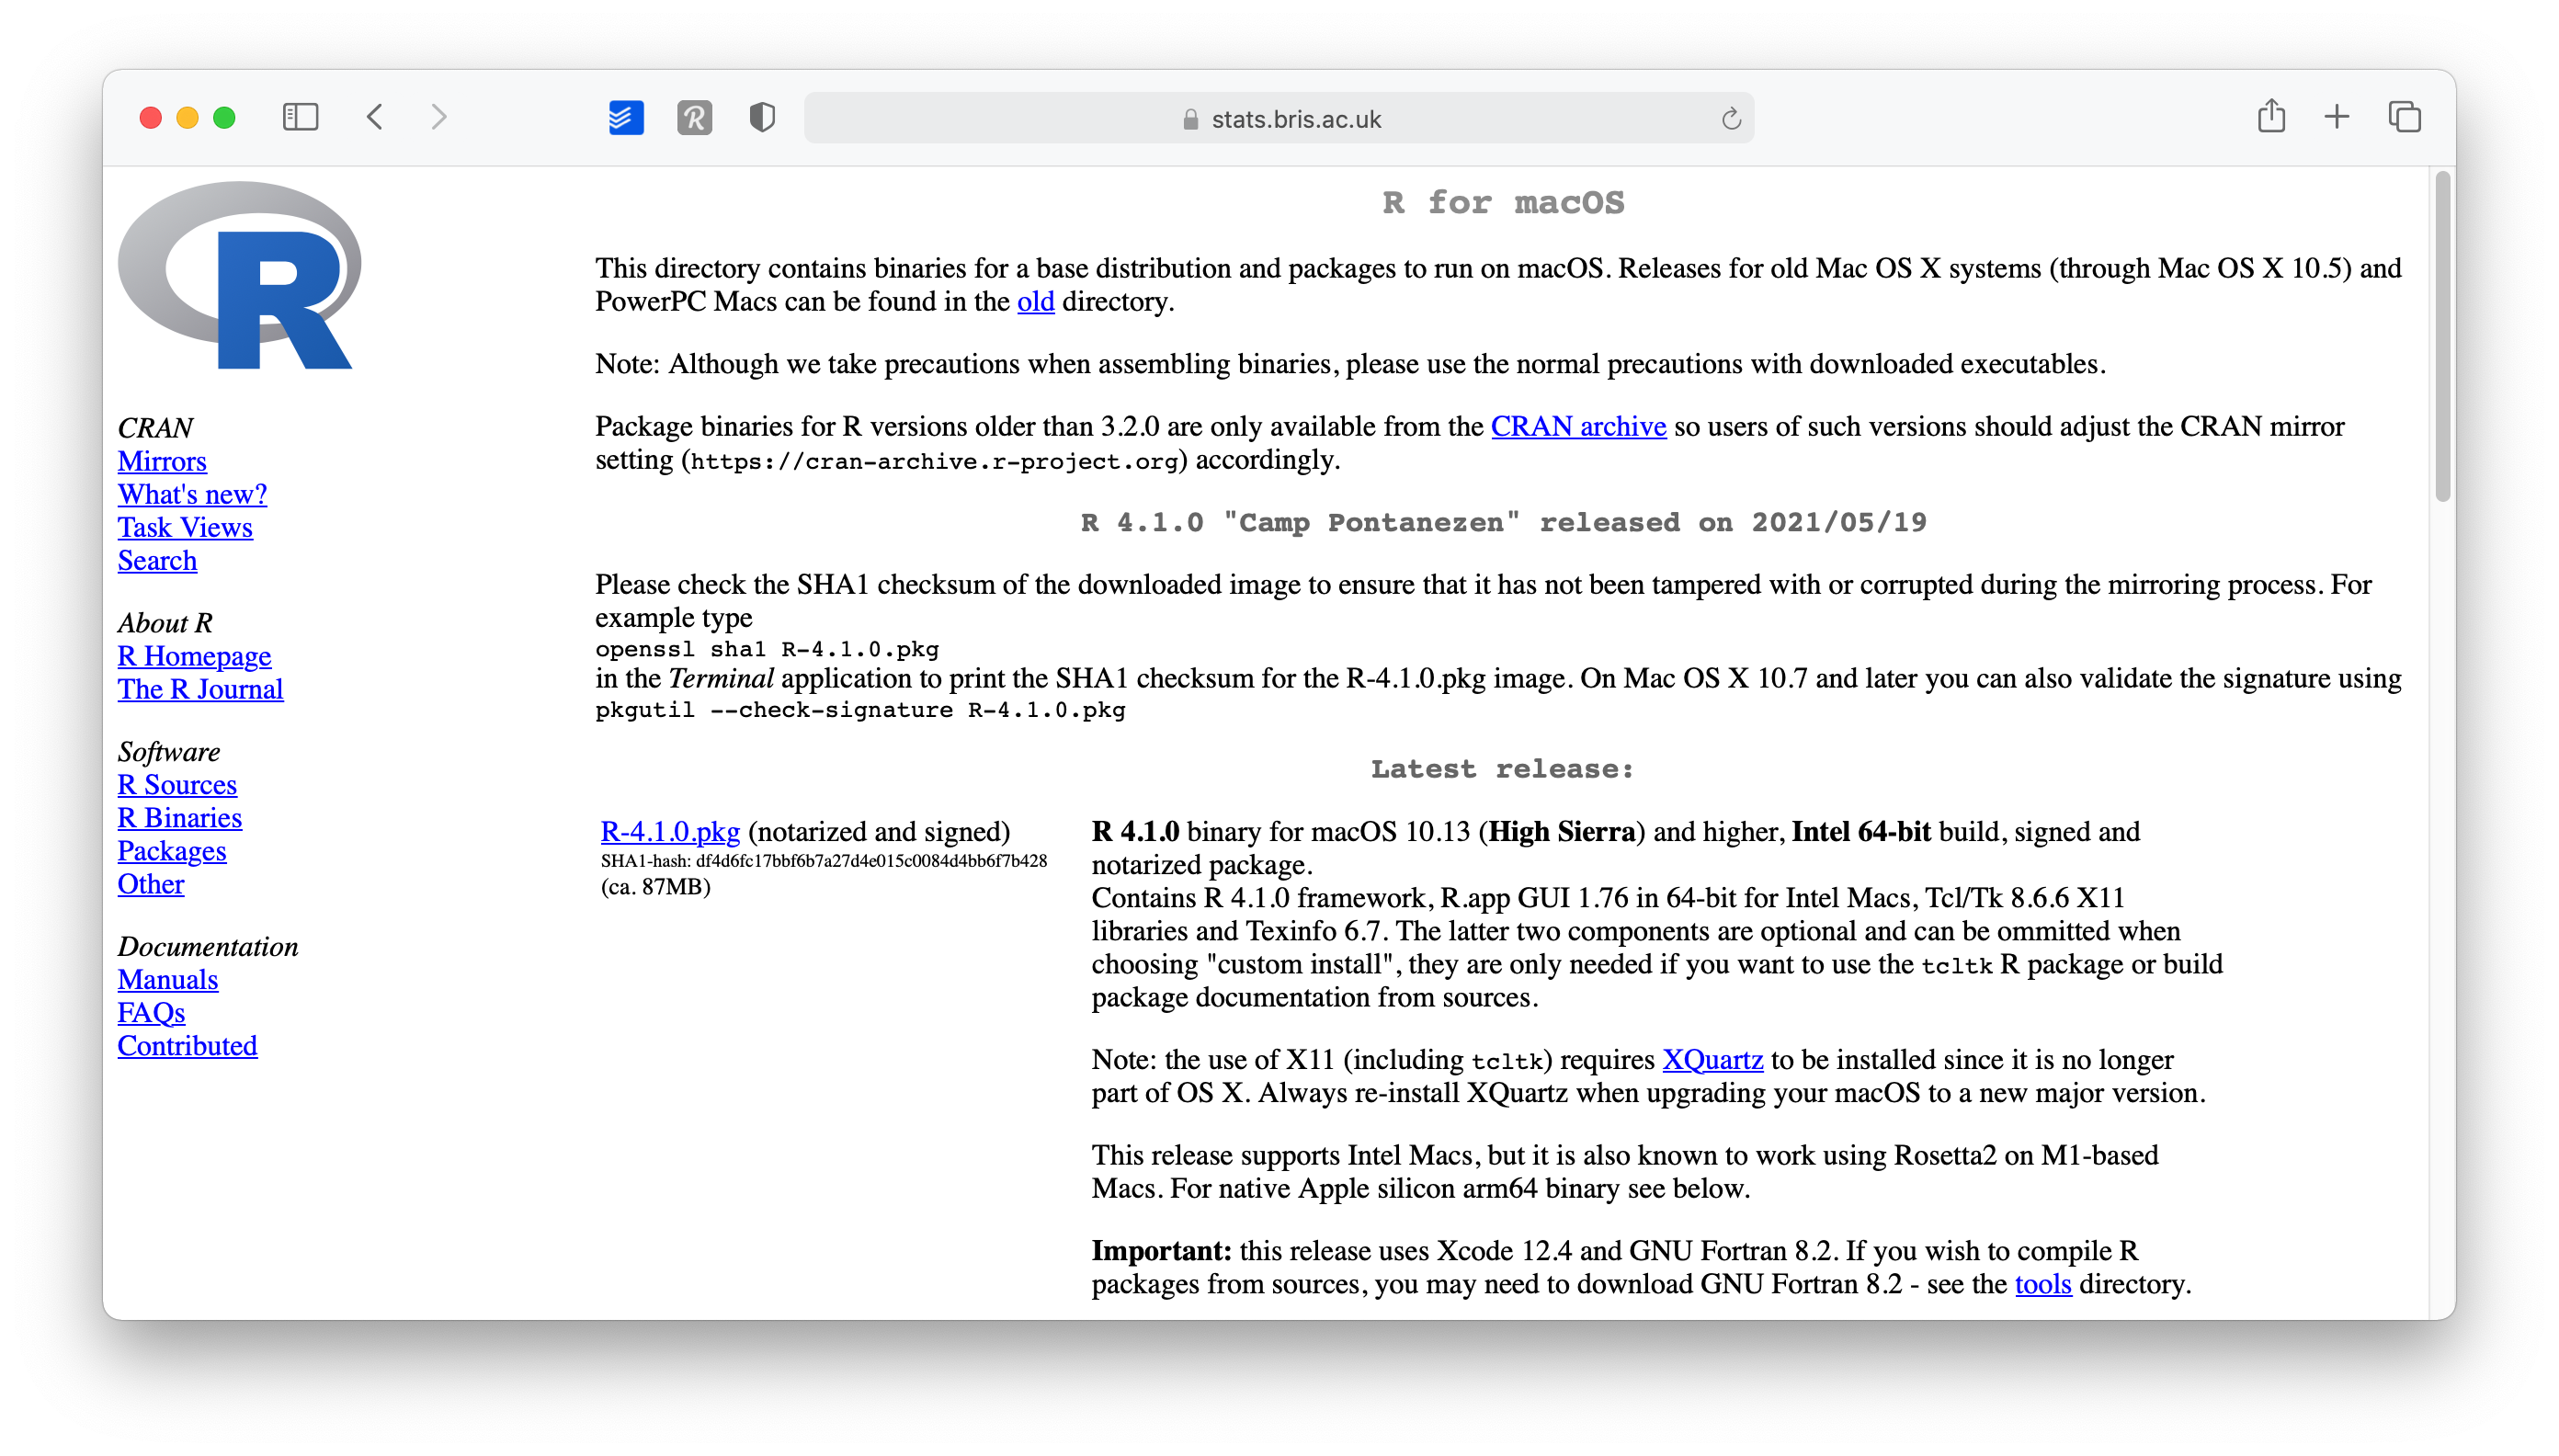
\includegraphics{images/chapter_03_img/r_project/03_r_project_version_choice.png}
\item
  Open the downloaded file and follow the installation instructions. (I recommend leaving the suggested settings as they are).
\end{enumerate}

This was relatively easy. You now have \emph{R} installed. Technically you can start using \emph{R} for your research, but there is one more tool I strongly advise installing: RStudio.

\hypertarget{installing-rstudio}{%
\section{Installing RStudio}\label{installing-rstudio}}

\emph{R} by itself is just the *`beating heart'* of \emph{R} programming, but it has no particular user interface. If you want buttons to click and actually `see' what you are doing, there is no better way than RStudio. RStudio is an \emph{integrated development environment} (IDE) and will be our primary tool to interact with \emph{R}. It is the only software you need to do all the fun parts and, of course, to follow along with the examples of this book. To install RStudio perform the following steps:

\begin{enumerate}
\def\labelenumi{\arabic{enumi}.}
\item
  Go to \href{https://www.rstudio.com\%5D(https://www.rstudio.com)}{www.rstudio.com}.

  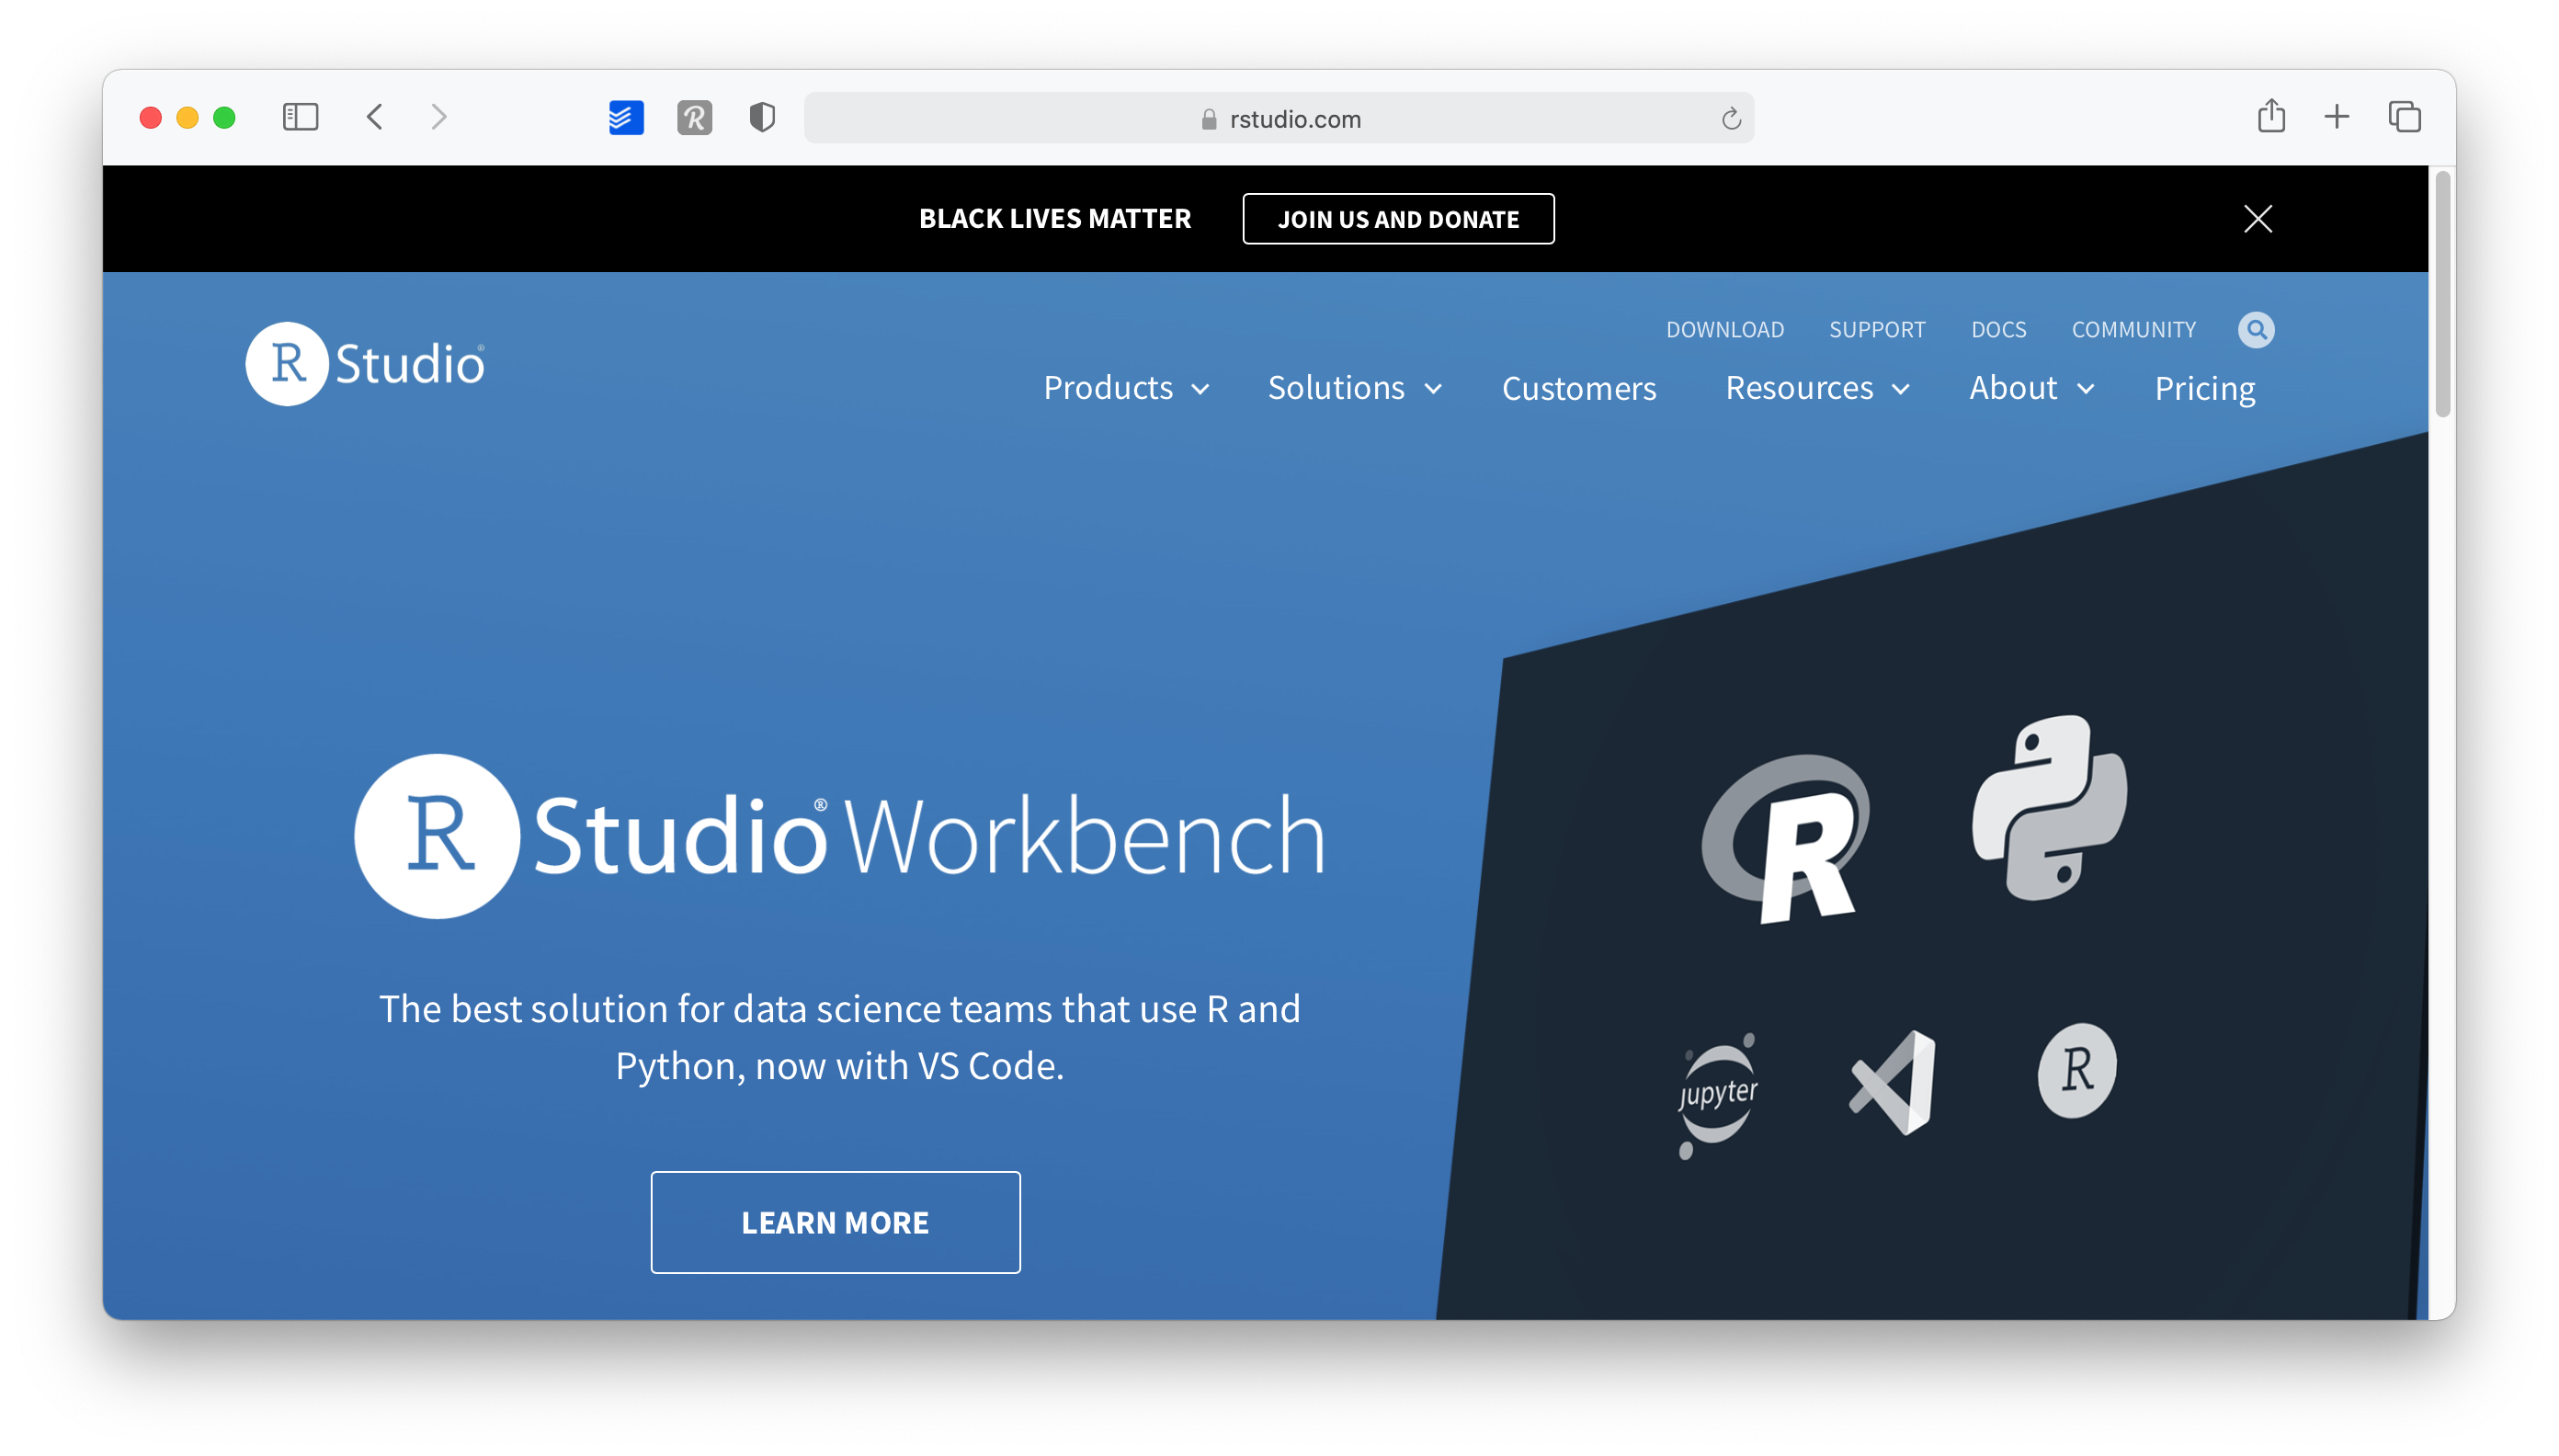
\includegraphics{images/chapter_03_img/rstudio/01_rstudio_main_page.png}
\item
  Go to \texttt{Products\ \textgreater{}\ RStudio}

  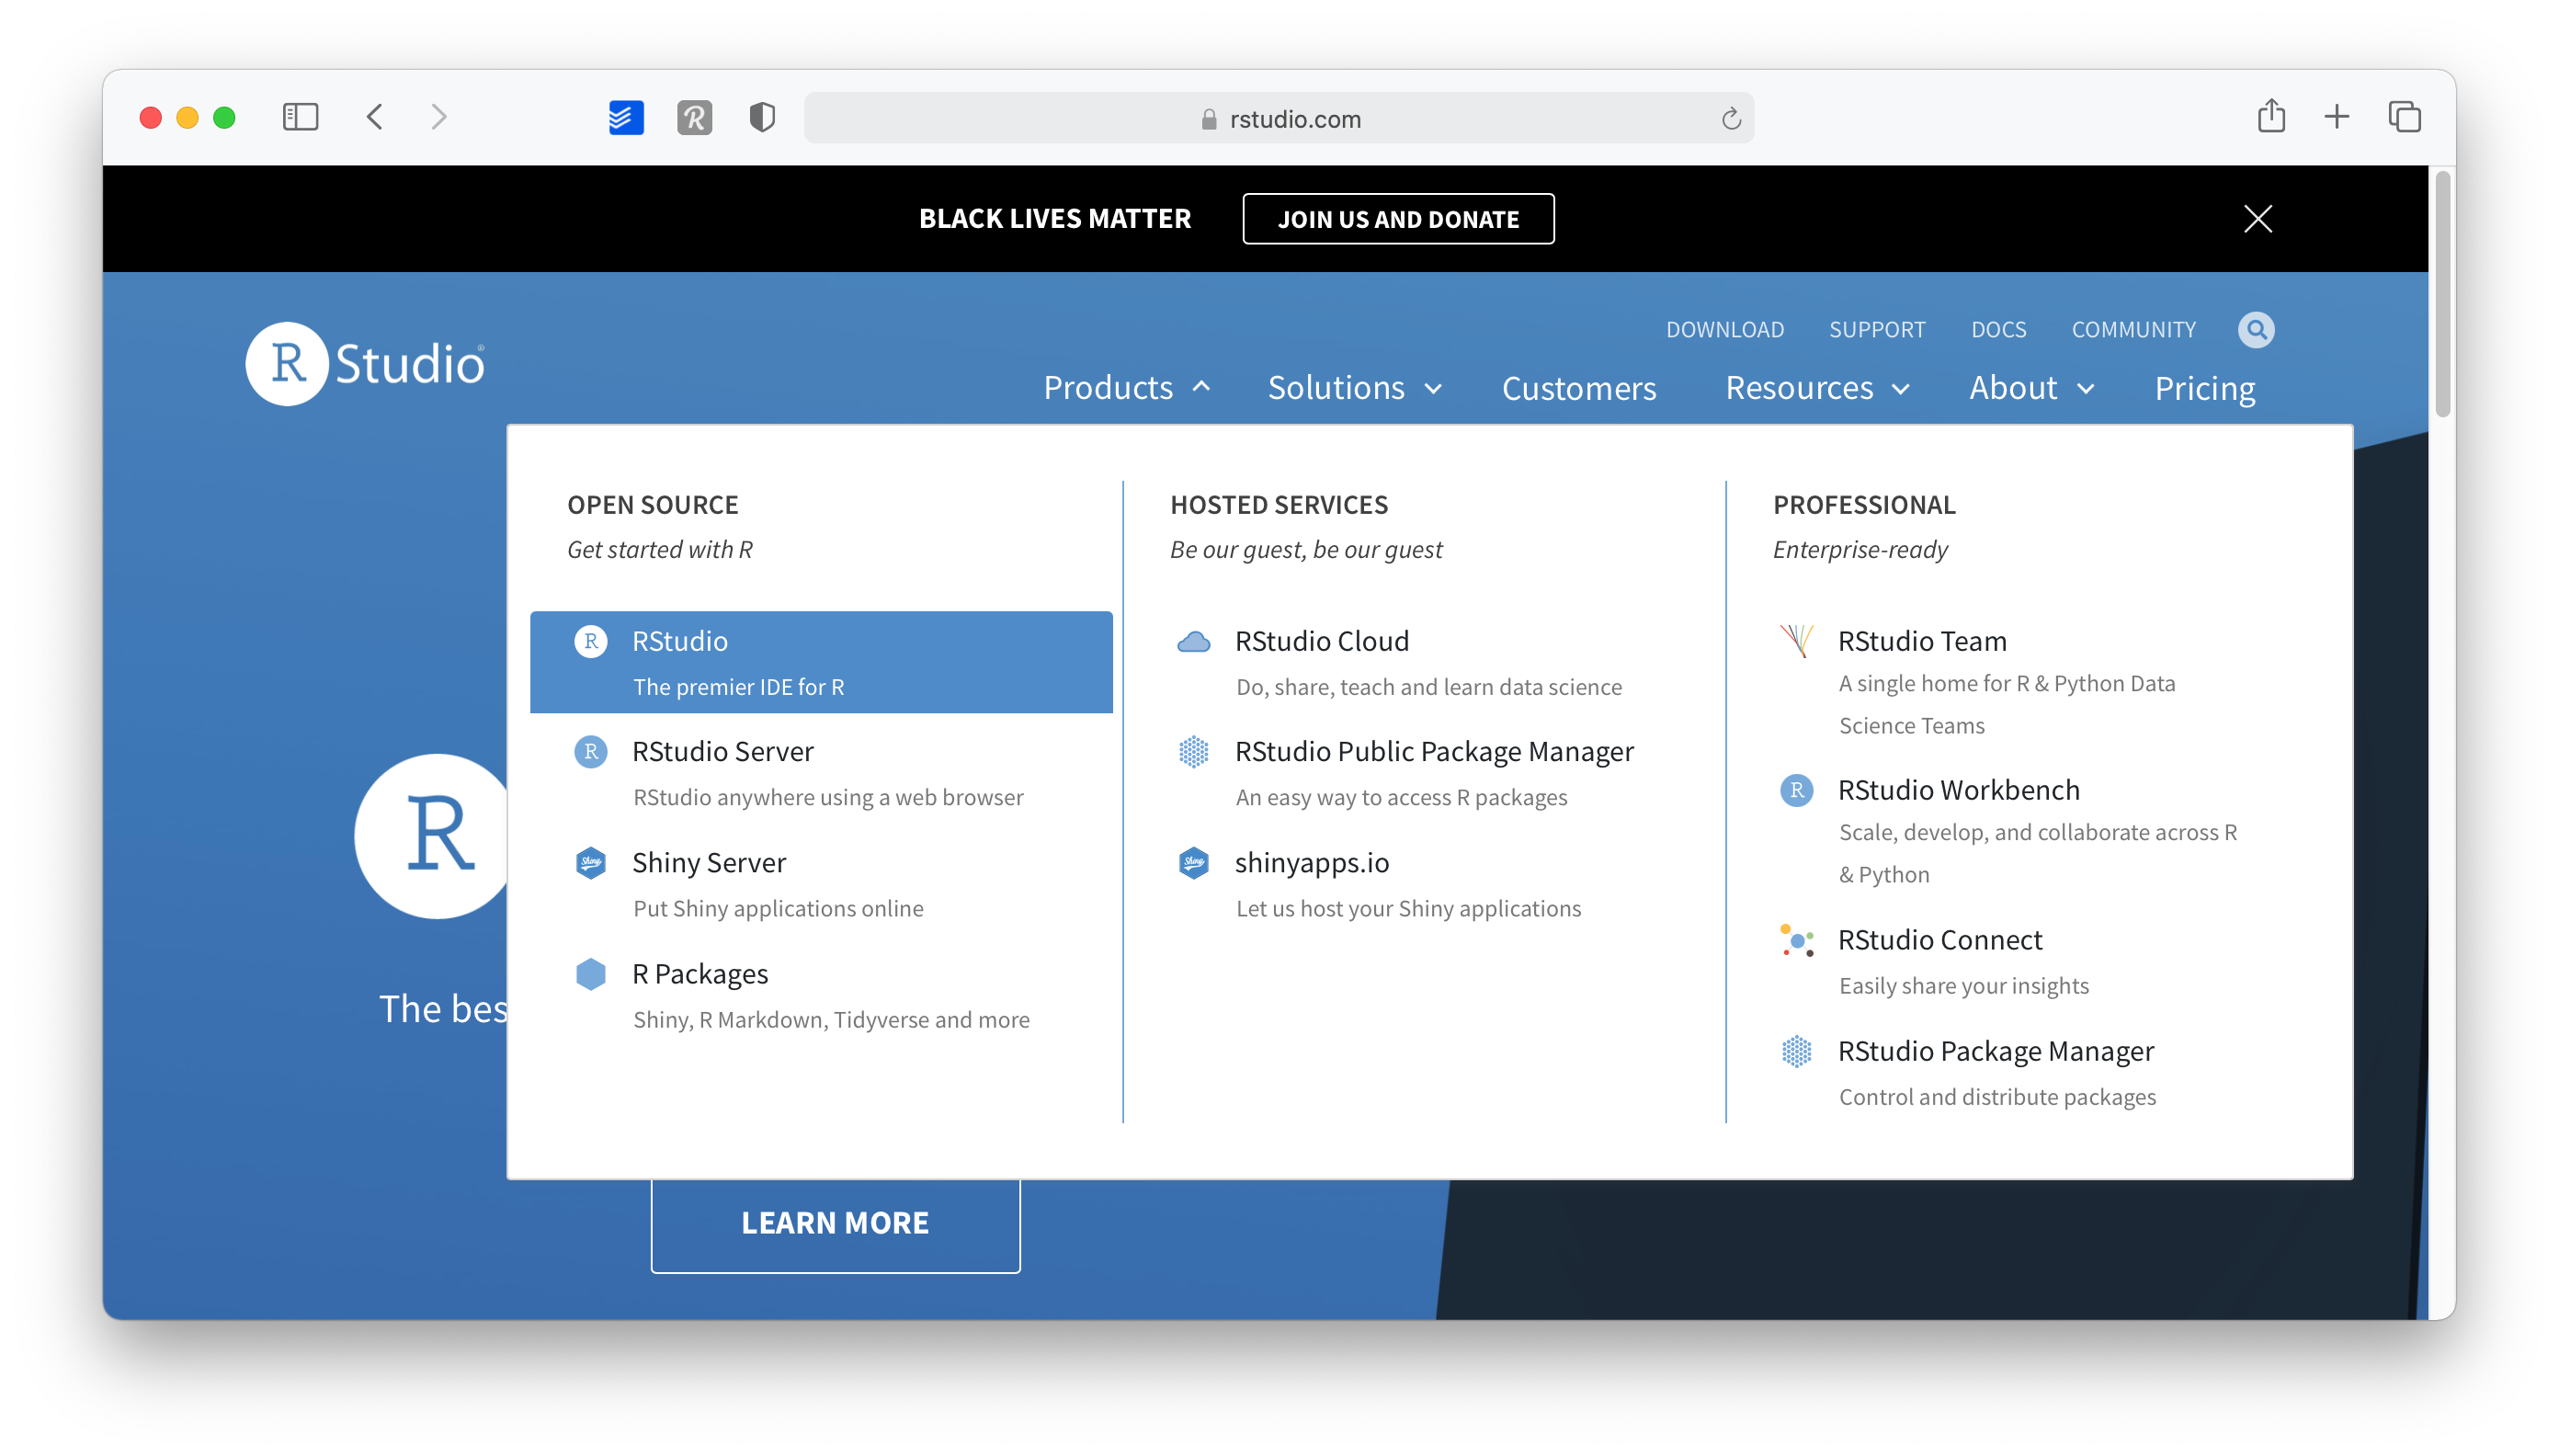
\includegraphics{images/chapter_03_img/rstudio/02_rstudio_main_page_menu.png}
\item
  On this page, scroll down and select \texttt{RStudio\ Desktop}

  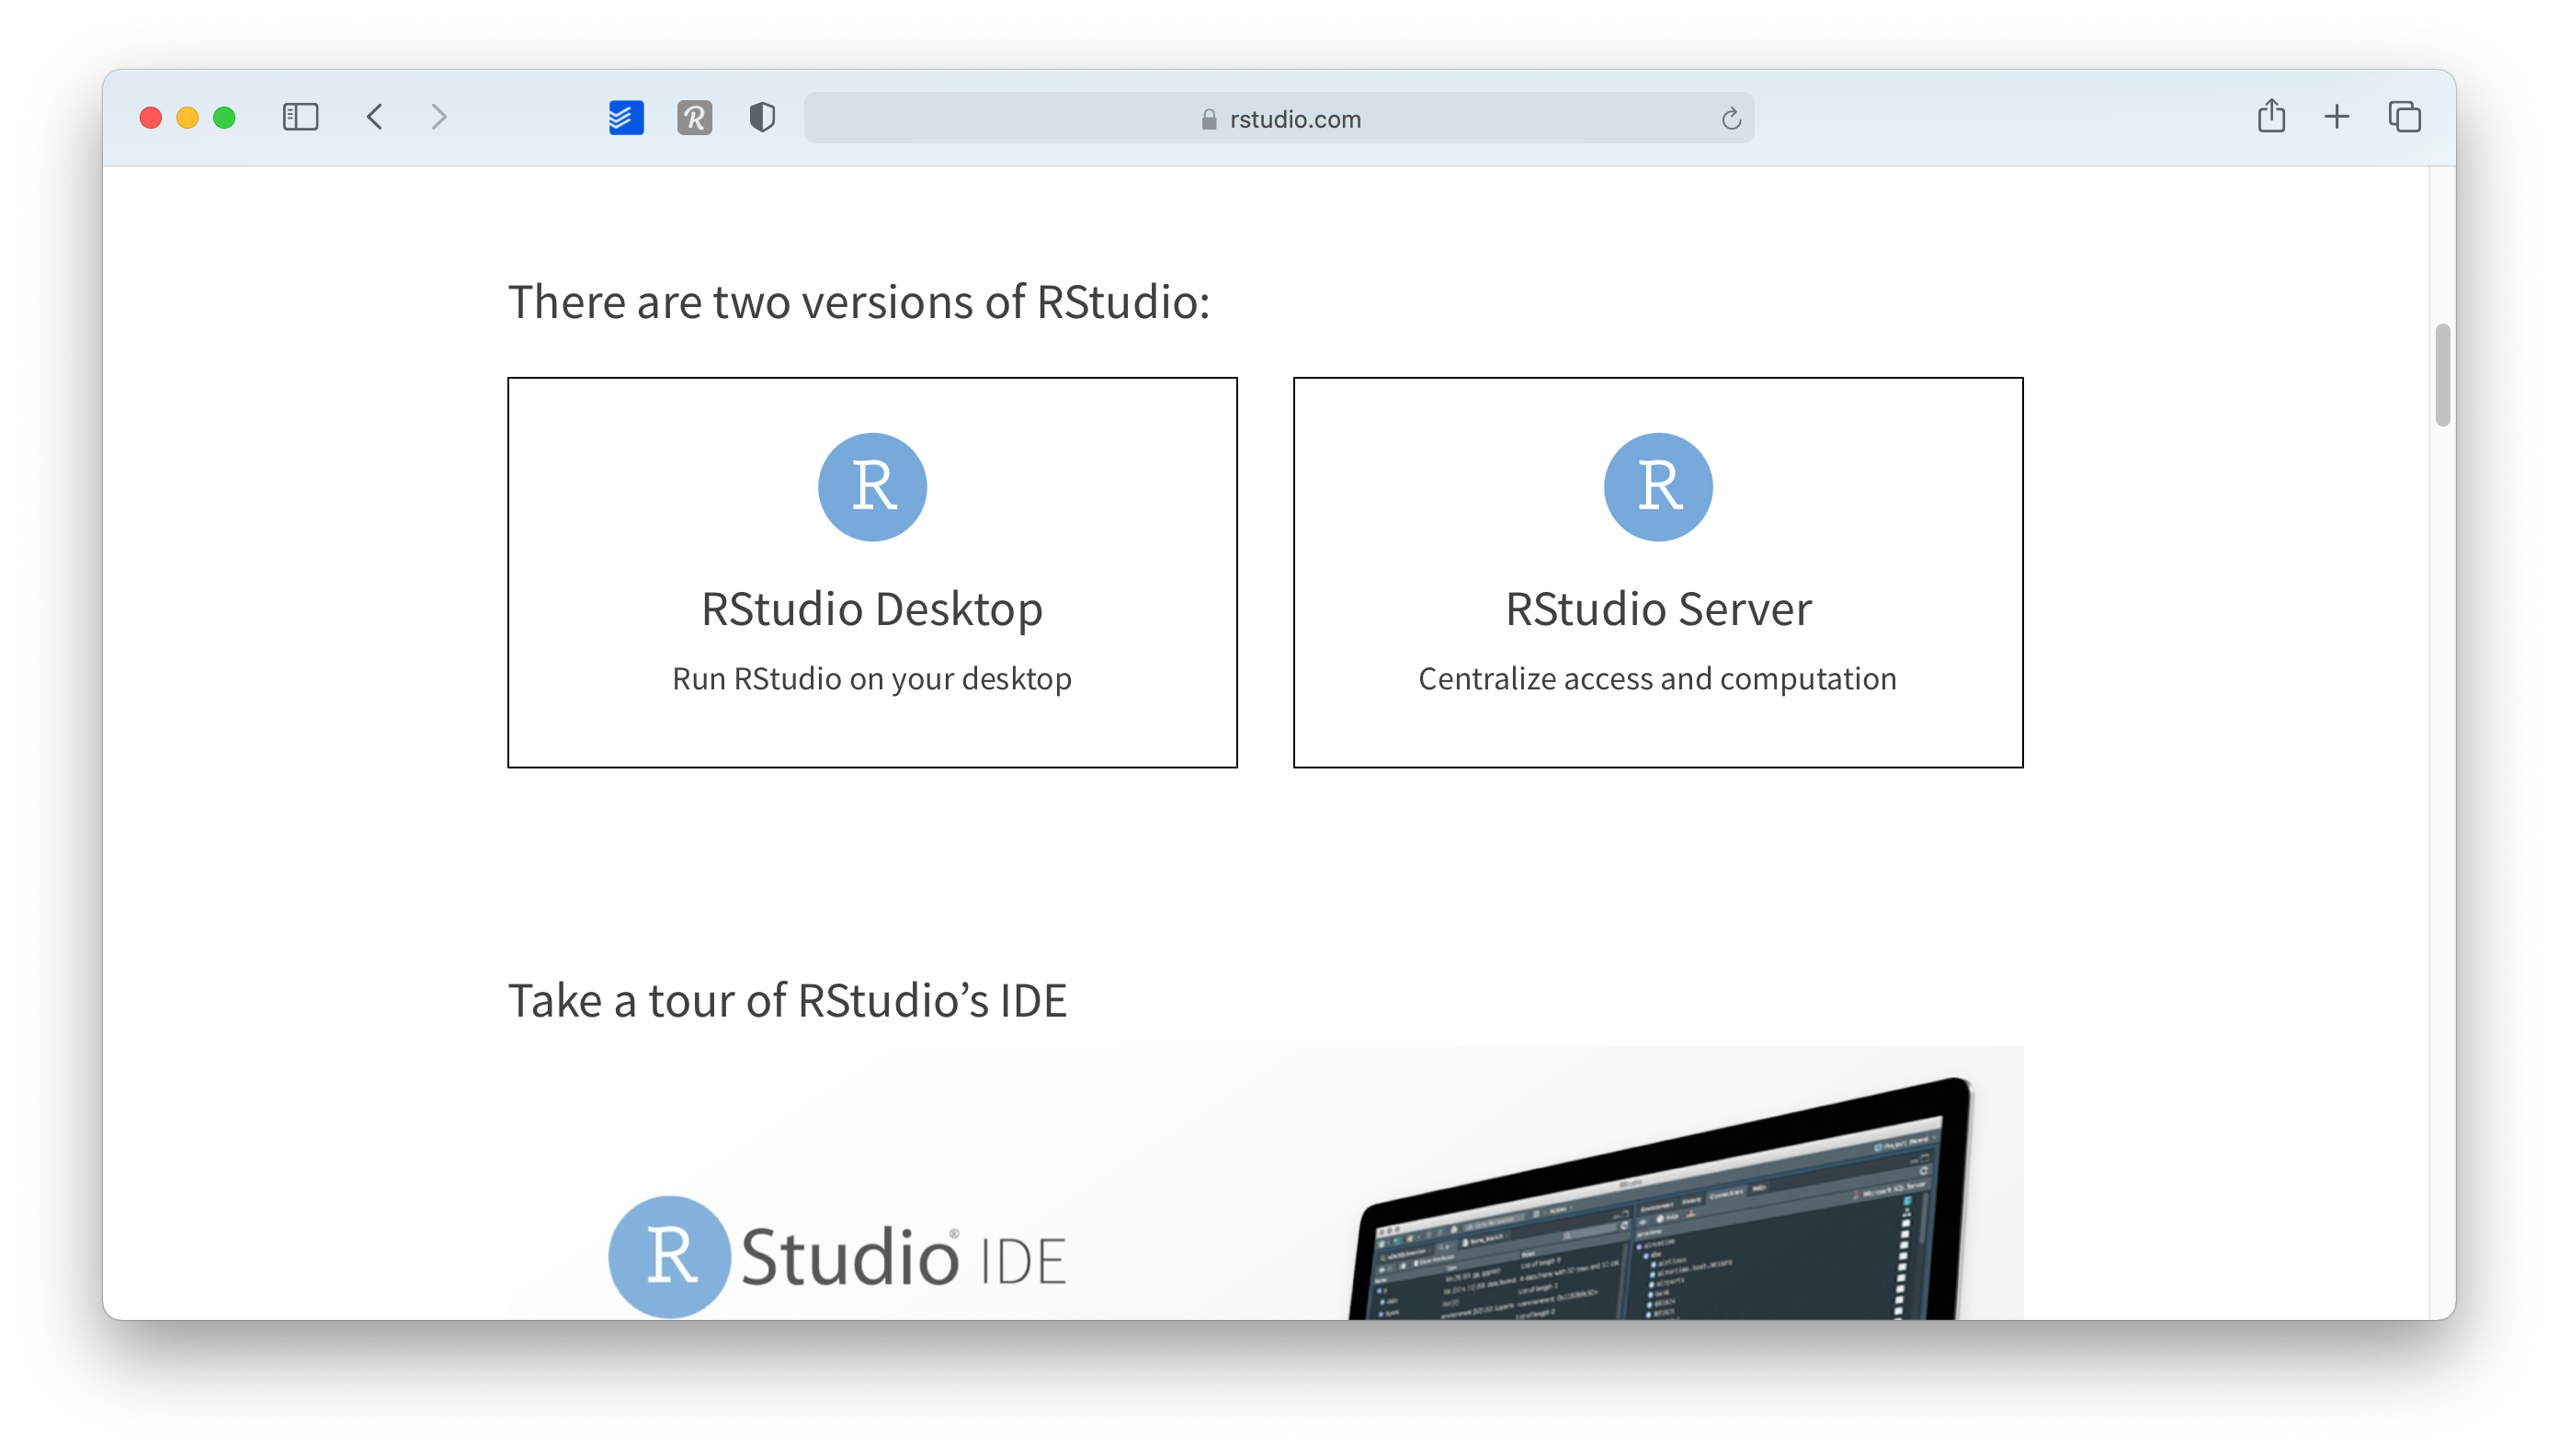
\includegraphics{images/chapter_03_img/rstudio/03_rstudio_select_version.png}
\item
  Select the \texttt{\textquotesingle{}Open\ Source\ Edition\textquotesingle{}} option by clicking on '\texttt{Download\ RStudio\ Desktop\textquotesingle{}}

  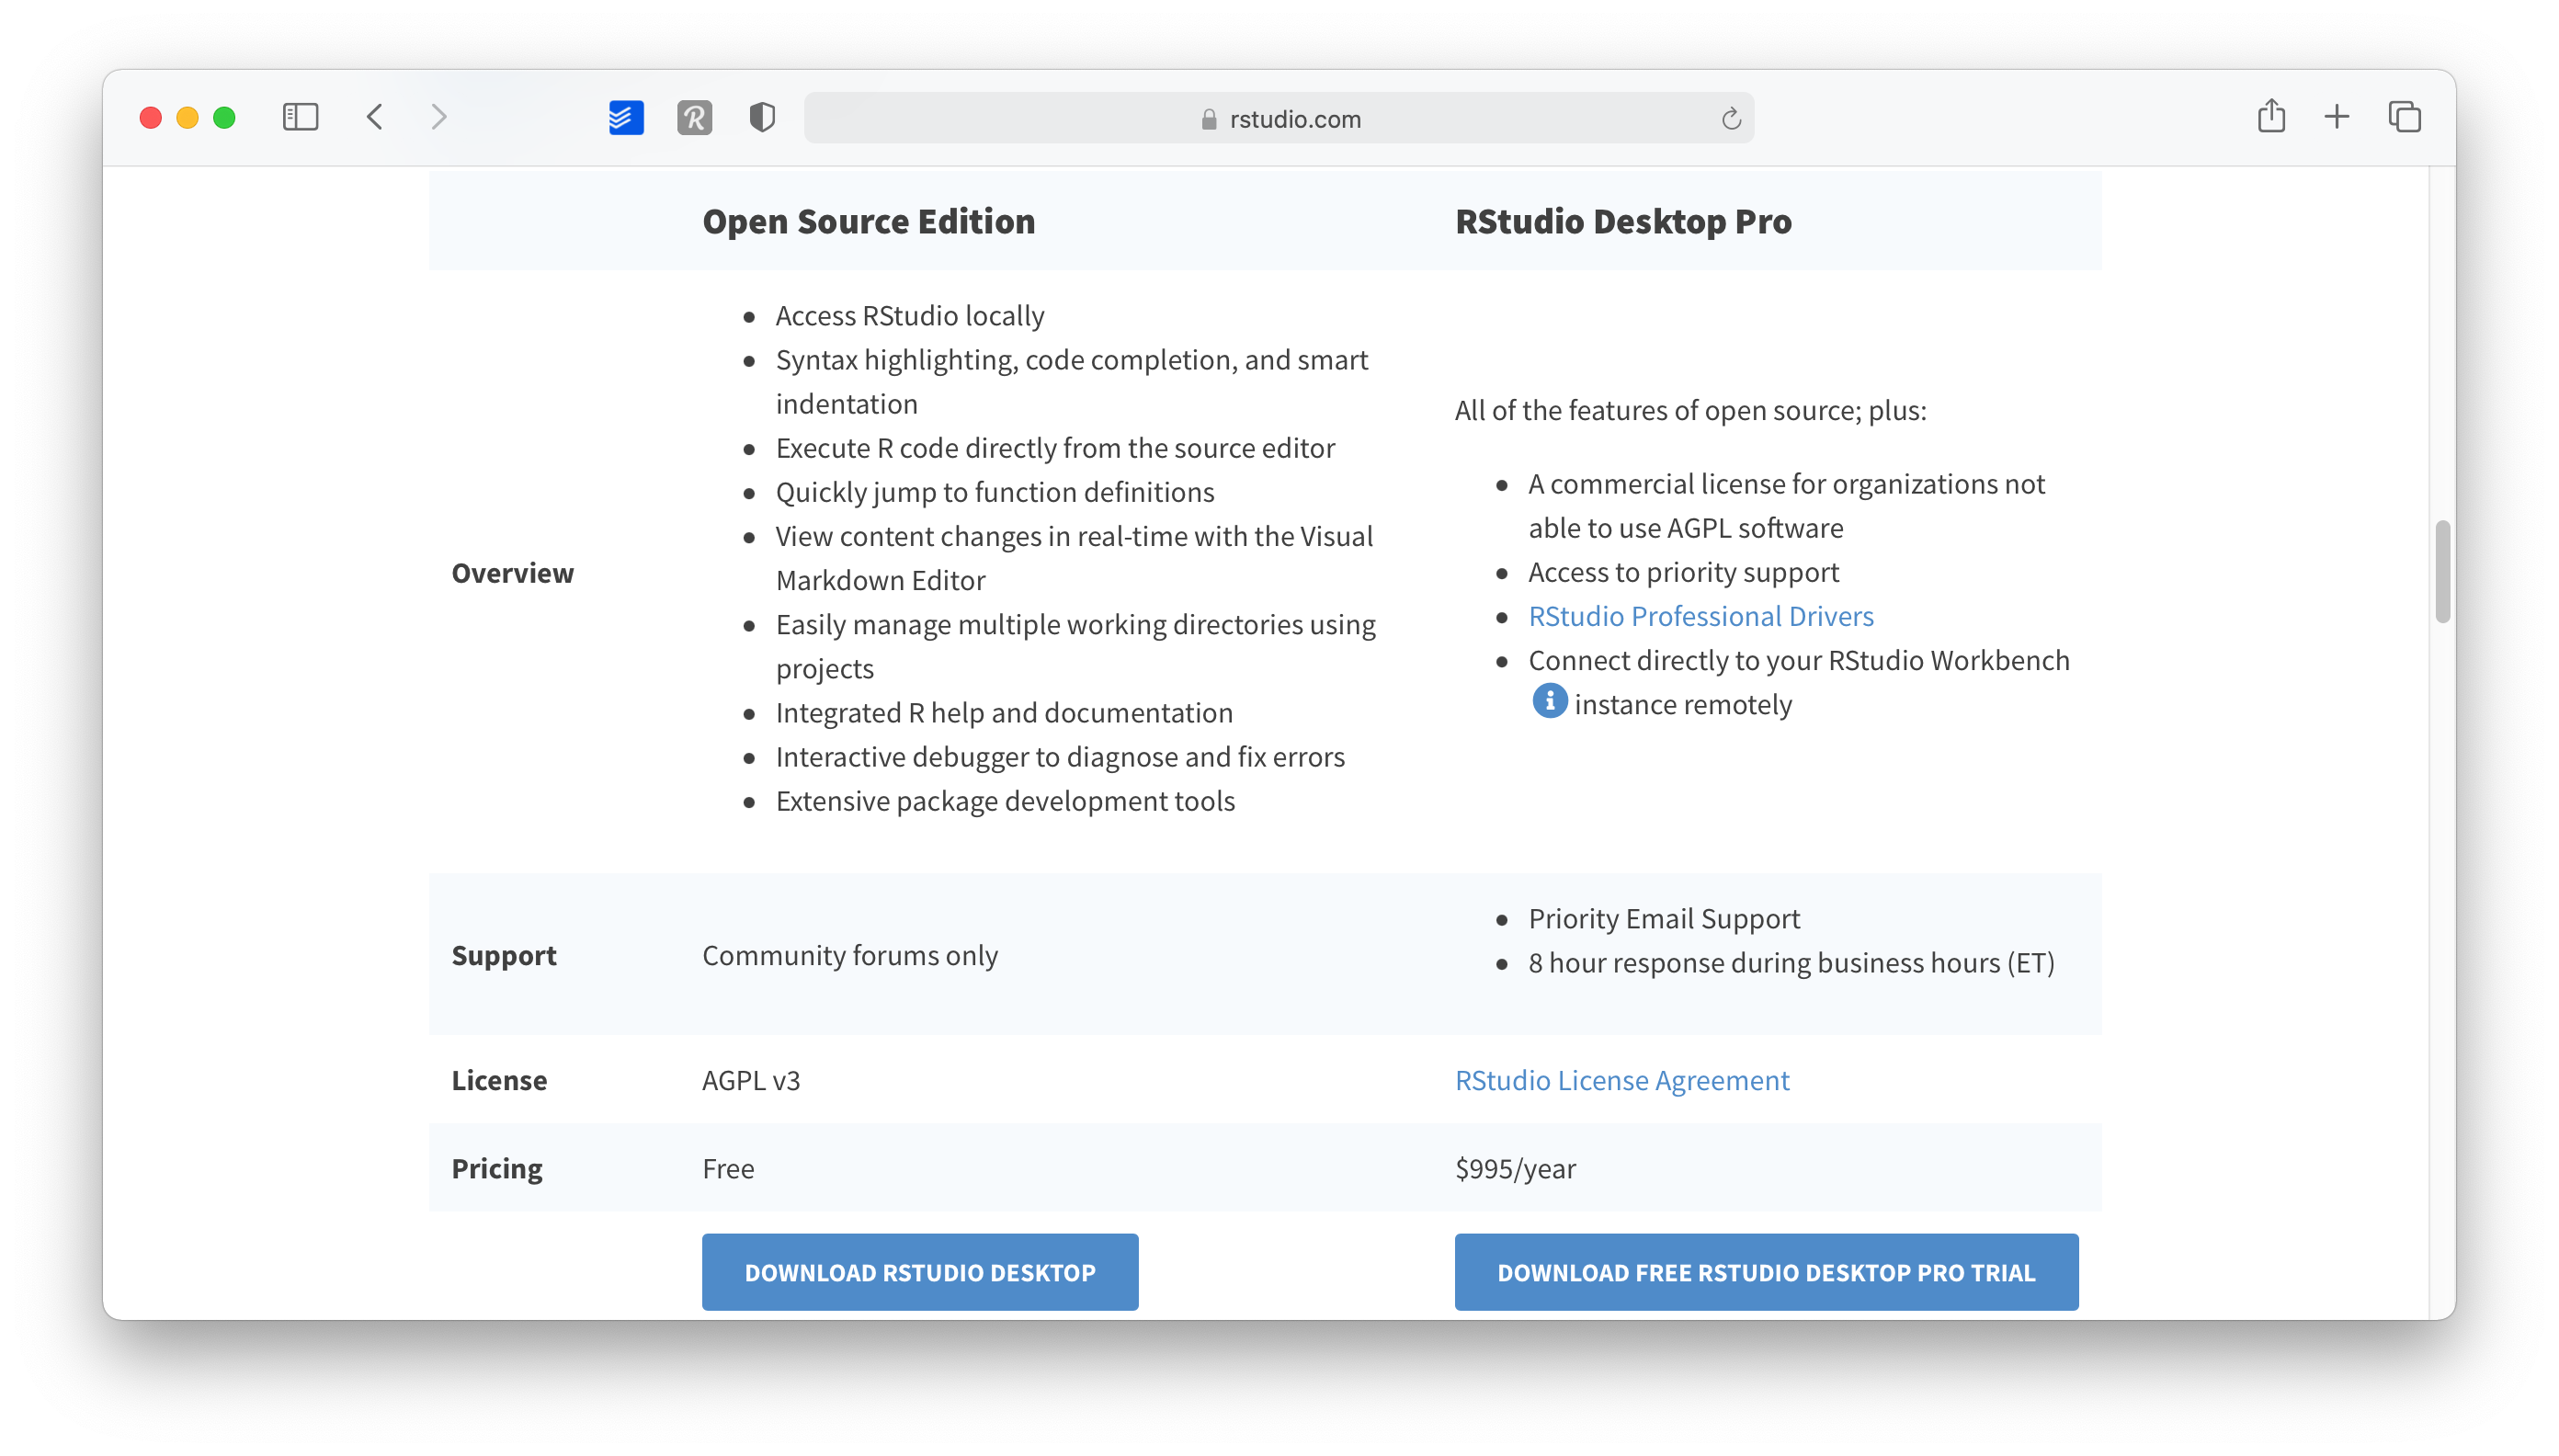
\includegraphics{images/chapter_03_img/rstudio/04_rstudio_select_edition.png}
\item
  As a last step, scroll down where it shows you a download button for your operating system. The website will automatically detect this. You also get a nice reminder to install `R' first, in case you have not done so yet.

  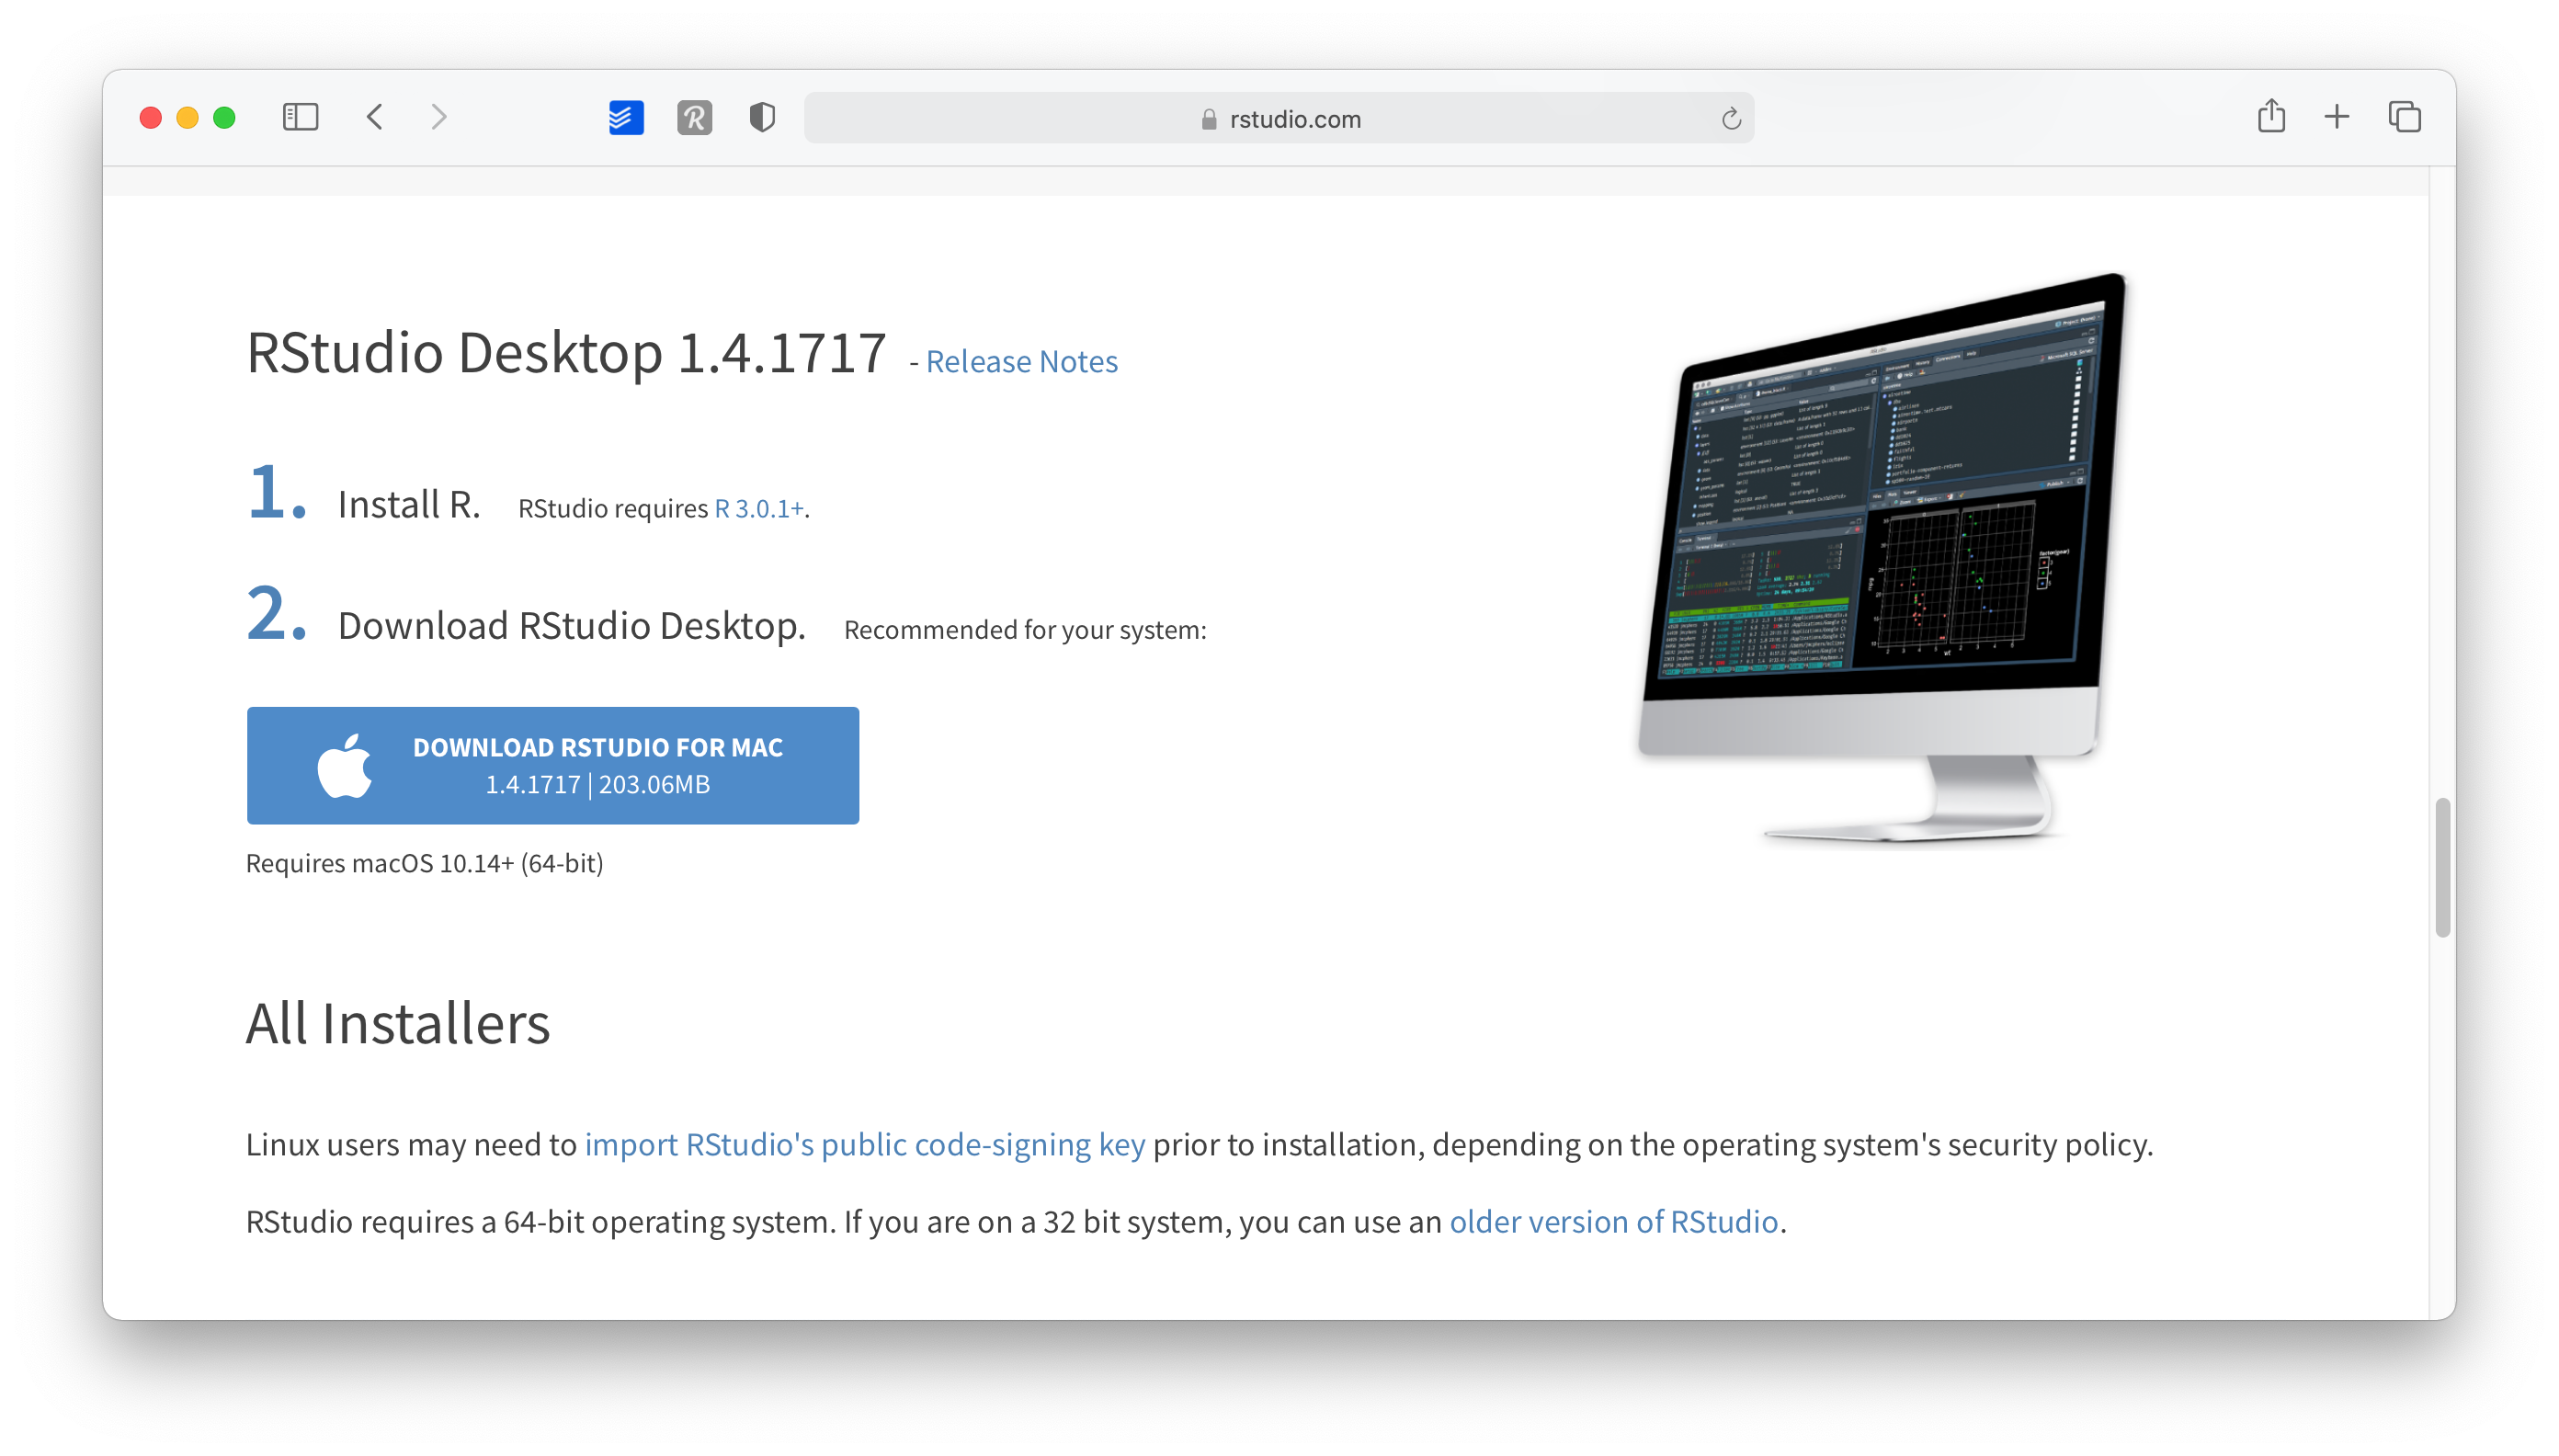
\includegraphics{images/chapter_03_img/rstudio/05_rstudio_download.png}
\item
  Open the downloaded file and follow the installation instructions (again, keep it to the default settings as much as possible)
\end{enumerate}

Congratulations, you are all set up to learn \emph{R}. From now on you only need to start RStudio and not \emph{R}. Of course, if you are the curious, nothing shall stop you to try \emph{R} without RStudio.

\hypertarget{when-you-first-start-rstudio}{%
\section{When you first start RStudio}\label{when-you-first-start-rstudio}}

Before you start programming away, you might want to make some tweaks to your settings right away to have a better experience (in my humble opinion). I recommend at least the following two changes by clicking on \texttt{RStudio\ \textgreater{}\ Preferences} or press \texttt{⌘/Ctrl\ +\ ,}.

\begin{enumerate}
\def\labelenumi{\arabic{enumi}.}
\item
  In the \texttt{Code\ \textgreater{}\ Editing} tab, make sure to have at least the first five options ticked, especially the \texttt{Auto-indent\ code\ after\ paste}. This setting will save time when trying to format your coding appropriately, making it easier to read. Indentation is the primary way of making your code look more readable and less like a series of characters that appear almost random.

  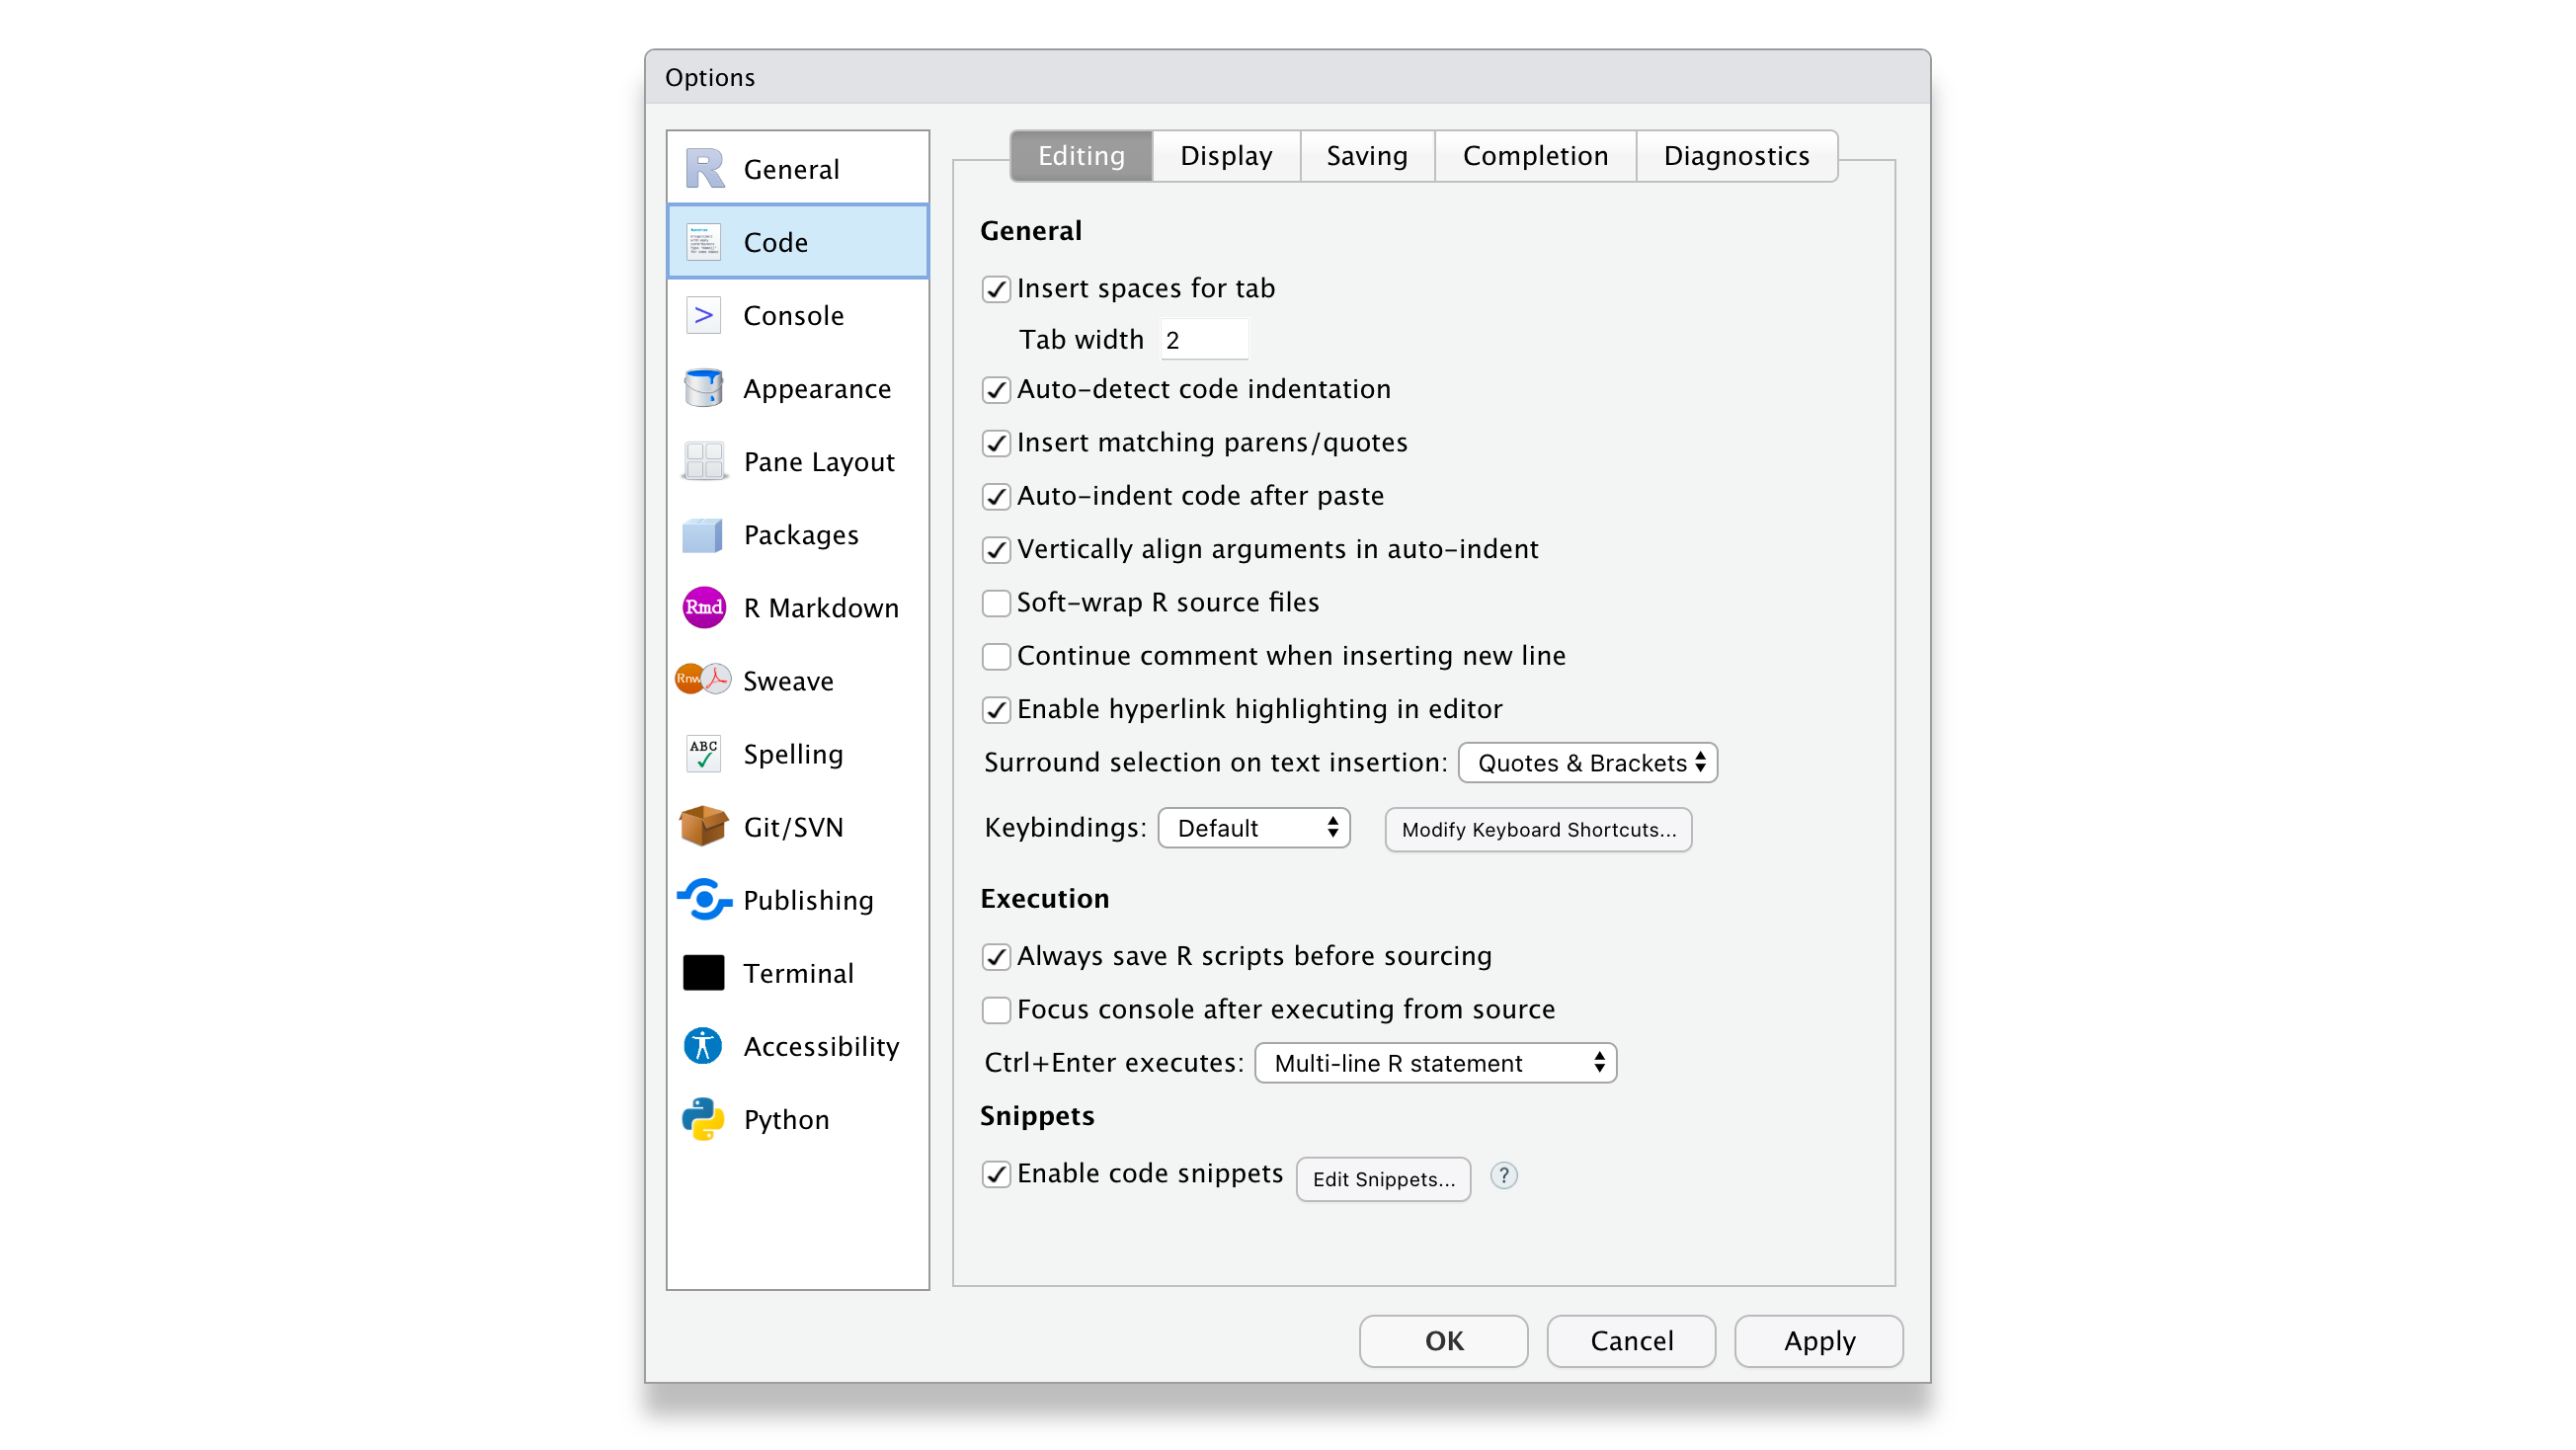
\includegraphics{images/chapter_03_img/rstudio_preferences/00_rstudio_preferences_editing.png}
\item
  In the \texttt{Display} tab, you might want to have the first three options selected. In particular, \texttt{Highlight\ selected\ line} is helpful because, in more complicated code, it is helpful to see where your cursor is.

  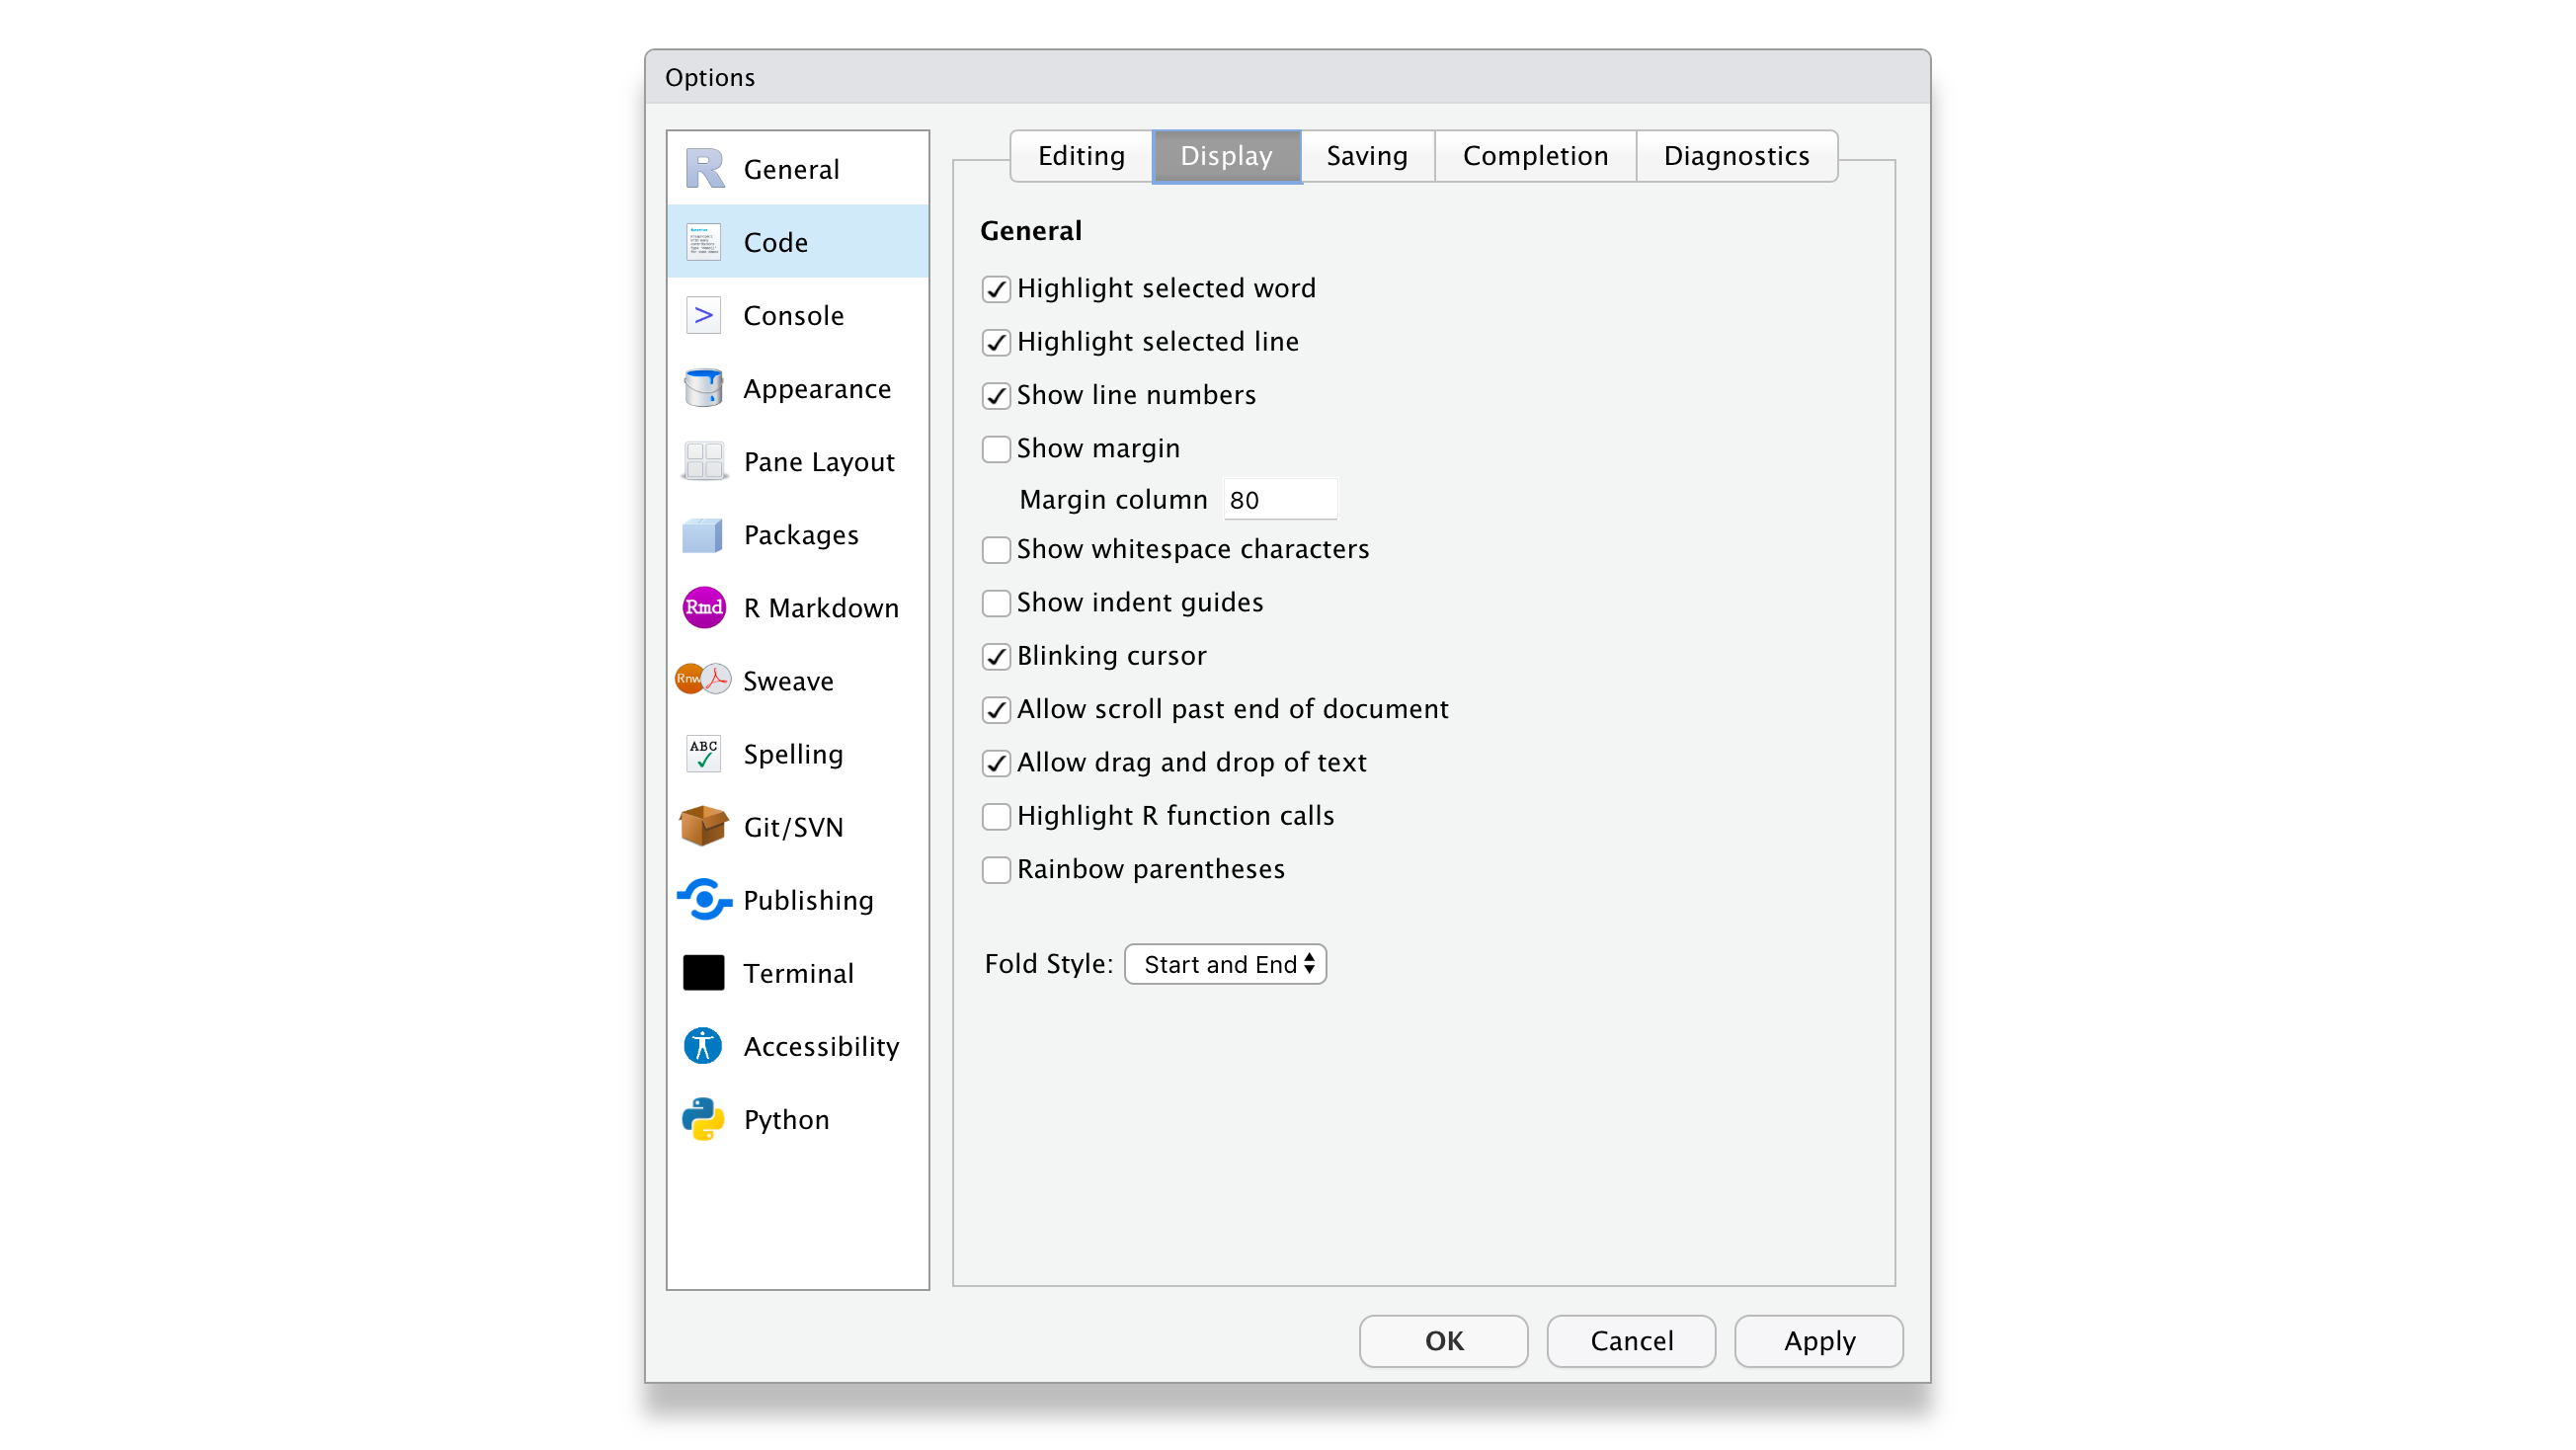
\includegraphics{images/chapter_03_img/rstudio_preferences/01_rstudio_preferences_display.png}
\end{enumerate}

Of course, if you wish to customise your workspace further, you can do so. The visually most impactful way to alter the default appearance of RStudio is to select Appearance and pick a completely different colour theme. Feel free to browse through various options and see what you prefer. There is no right or wrong here.

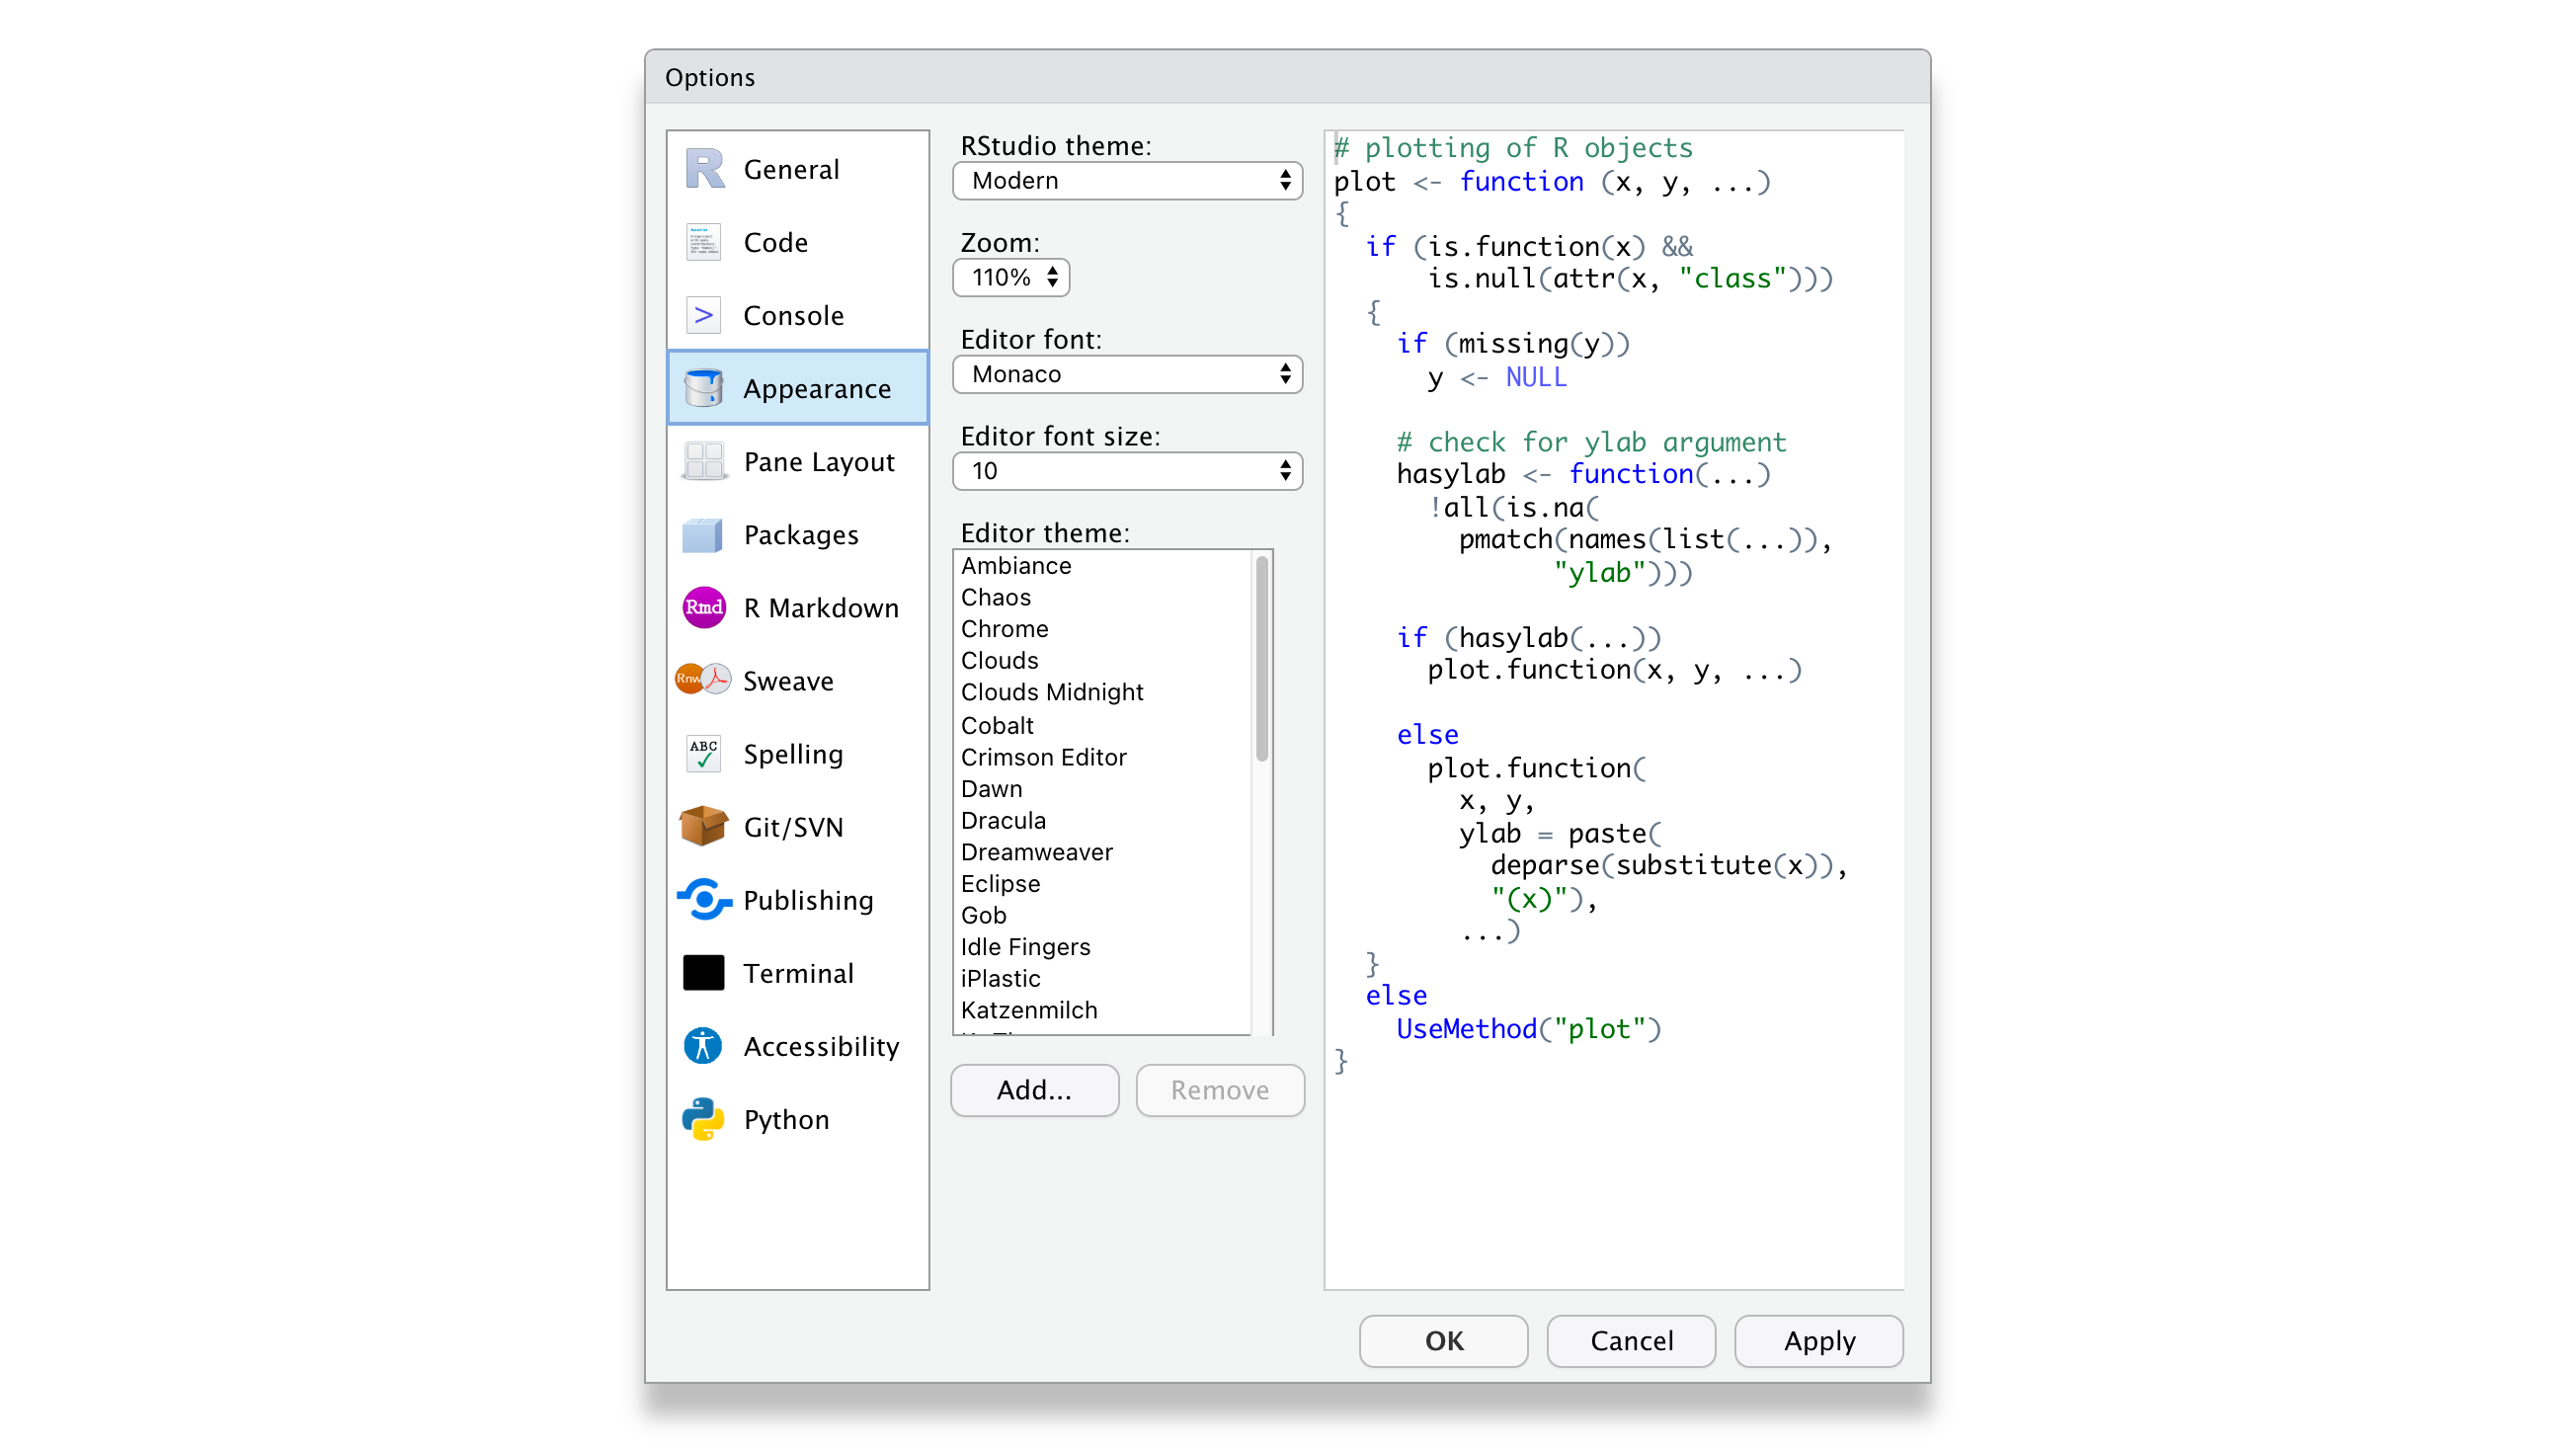
\includegraphics{images/chapter_03_img/rstudio_preferences/02_rstudio_preferences_appearance.png}

\hypertarget{updating-r-and-rstudio}{%
\section{Updating R and RStudio: Living at the pulse of innovation}\label{updating-r-and-rstudio}}

While not strictly something that helps you become a better programmer, this advice might come in handy to avoid turning into a frustrated programmer. When you update your software, you need to update R and RStudio separately from each other. While both R and RStudio work closely with each other, they still constitute separate pieces of software. Thus, it is essential to keep in mind that updating RStudio will not automatically update R. This can become problematic if specific packages you installed via RStudio (like a fancy learning algorithm) might not be compatible with earlier versions of R. Also, additional R packages developed by other people are separate pieces and are updated too, independently from R and RStudio.

I know what you are thinking: This already sounds complicated and cumbersome. However, rest assured, we take a look at how you can easily update all your packages with RStudio. Thus, all you need to remember is:~\emph{R}~needs to be updated separately from everything else.

\hypertarget{rstudio-cloud}{%
\section{RStudio Cloud}\label{rstudio-cloud}}

\texttt{to\ be\ completed}

\hypertarget{the-rstudio-interface}{%
\chapter{The RStudio Interface}\label{the-rstudio-interface}}

The RStudio interface is composed of quadrants, each of which fulfils a unique purpose:

\begin{itemize}
\item
  The \texttt{Console} window,
\item
  The \texttt{Source} window,
\item
  The \texttt{Environment\ /\ History\ /\ Connections\ /\ Tutorial} window, and
\item
  The \texttt{Files\ /\ Plots\ /\ Packages\ /\ Help\ /\ Viewer} window
\end{itemize}

You might only see three windows and wonder where the \texttt{Source} window has gone in your version of RStudio. In order to use it you have to either open a file or create a new one. You can create a new file by selecting \texttt{File\ \textgreater{}\ New\ File\ \textgreater{}\ R\ Script} in the menu bar, or use the keyboard shortcut \texttt{Ctrl+Shift+N} on PC and \texttt{Cmd+Shift+N} on Mac.

I will briefly explain the purpose of each window/pane and how they are relevant to your work in \emph{R}.

\hypertarget{the-console-window}{%
\section{The Console window}\label{the-console-window}}

The console is located in the bottom-left, and it is where you often will find the output of your coding and computations. It is also possible to write code directly into the console. Let's try the following example by calculating the sum of \texttt{10\ +\ 5}. Click into the console with your mouse, type the calculation into your console and hit \texttt{Enter/Return\ ↵} on your keyboard. The result should be pretty obvious:

\begin{Shaded}
\begin{Highlighting}[]
\CommentTok{\# We type the below into the console 👇}
\DecValTok{10}\SpecialCharTok{+}\DecValTok{5}
\DocumentationTok{\#\# [1] 15}
\end{Highlighting}
\end{Shaded}

Here is a screenshot of how it should look like at your end in RStudio:

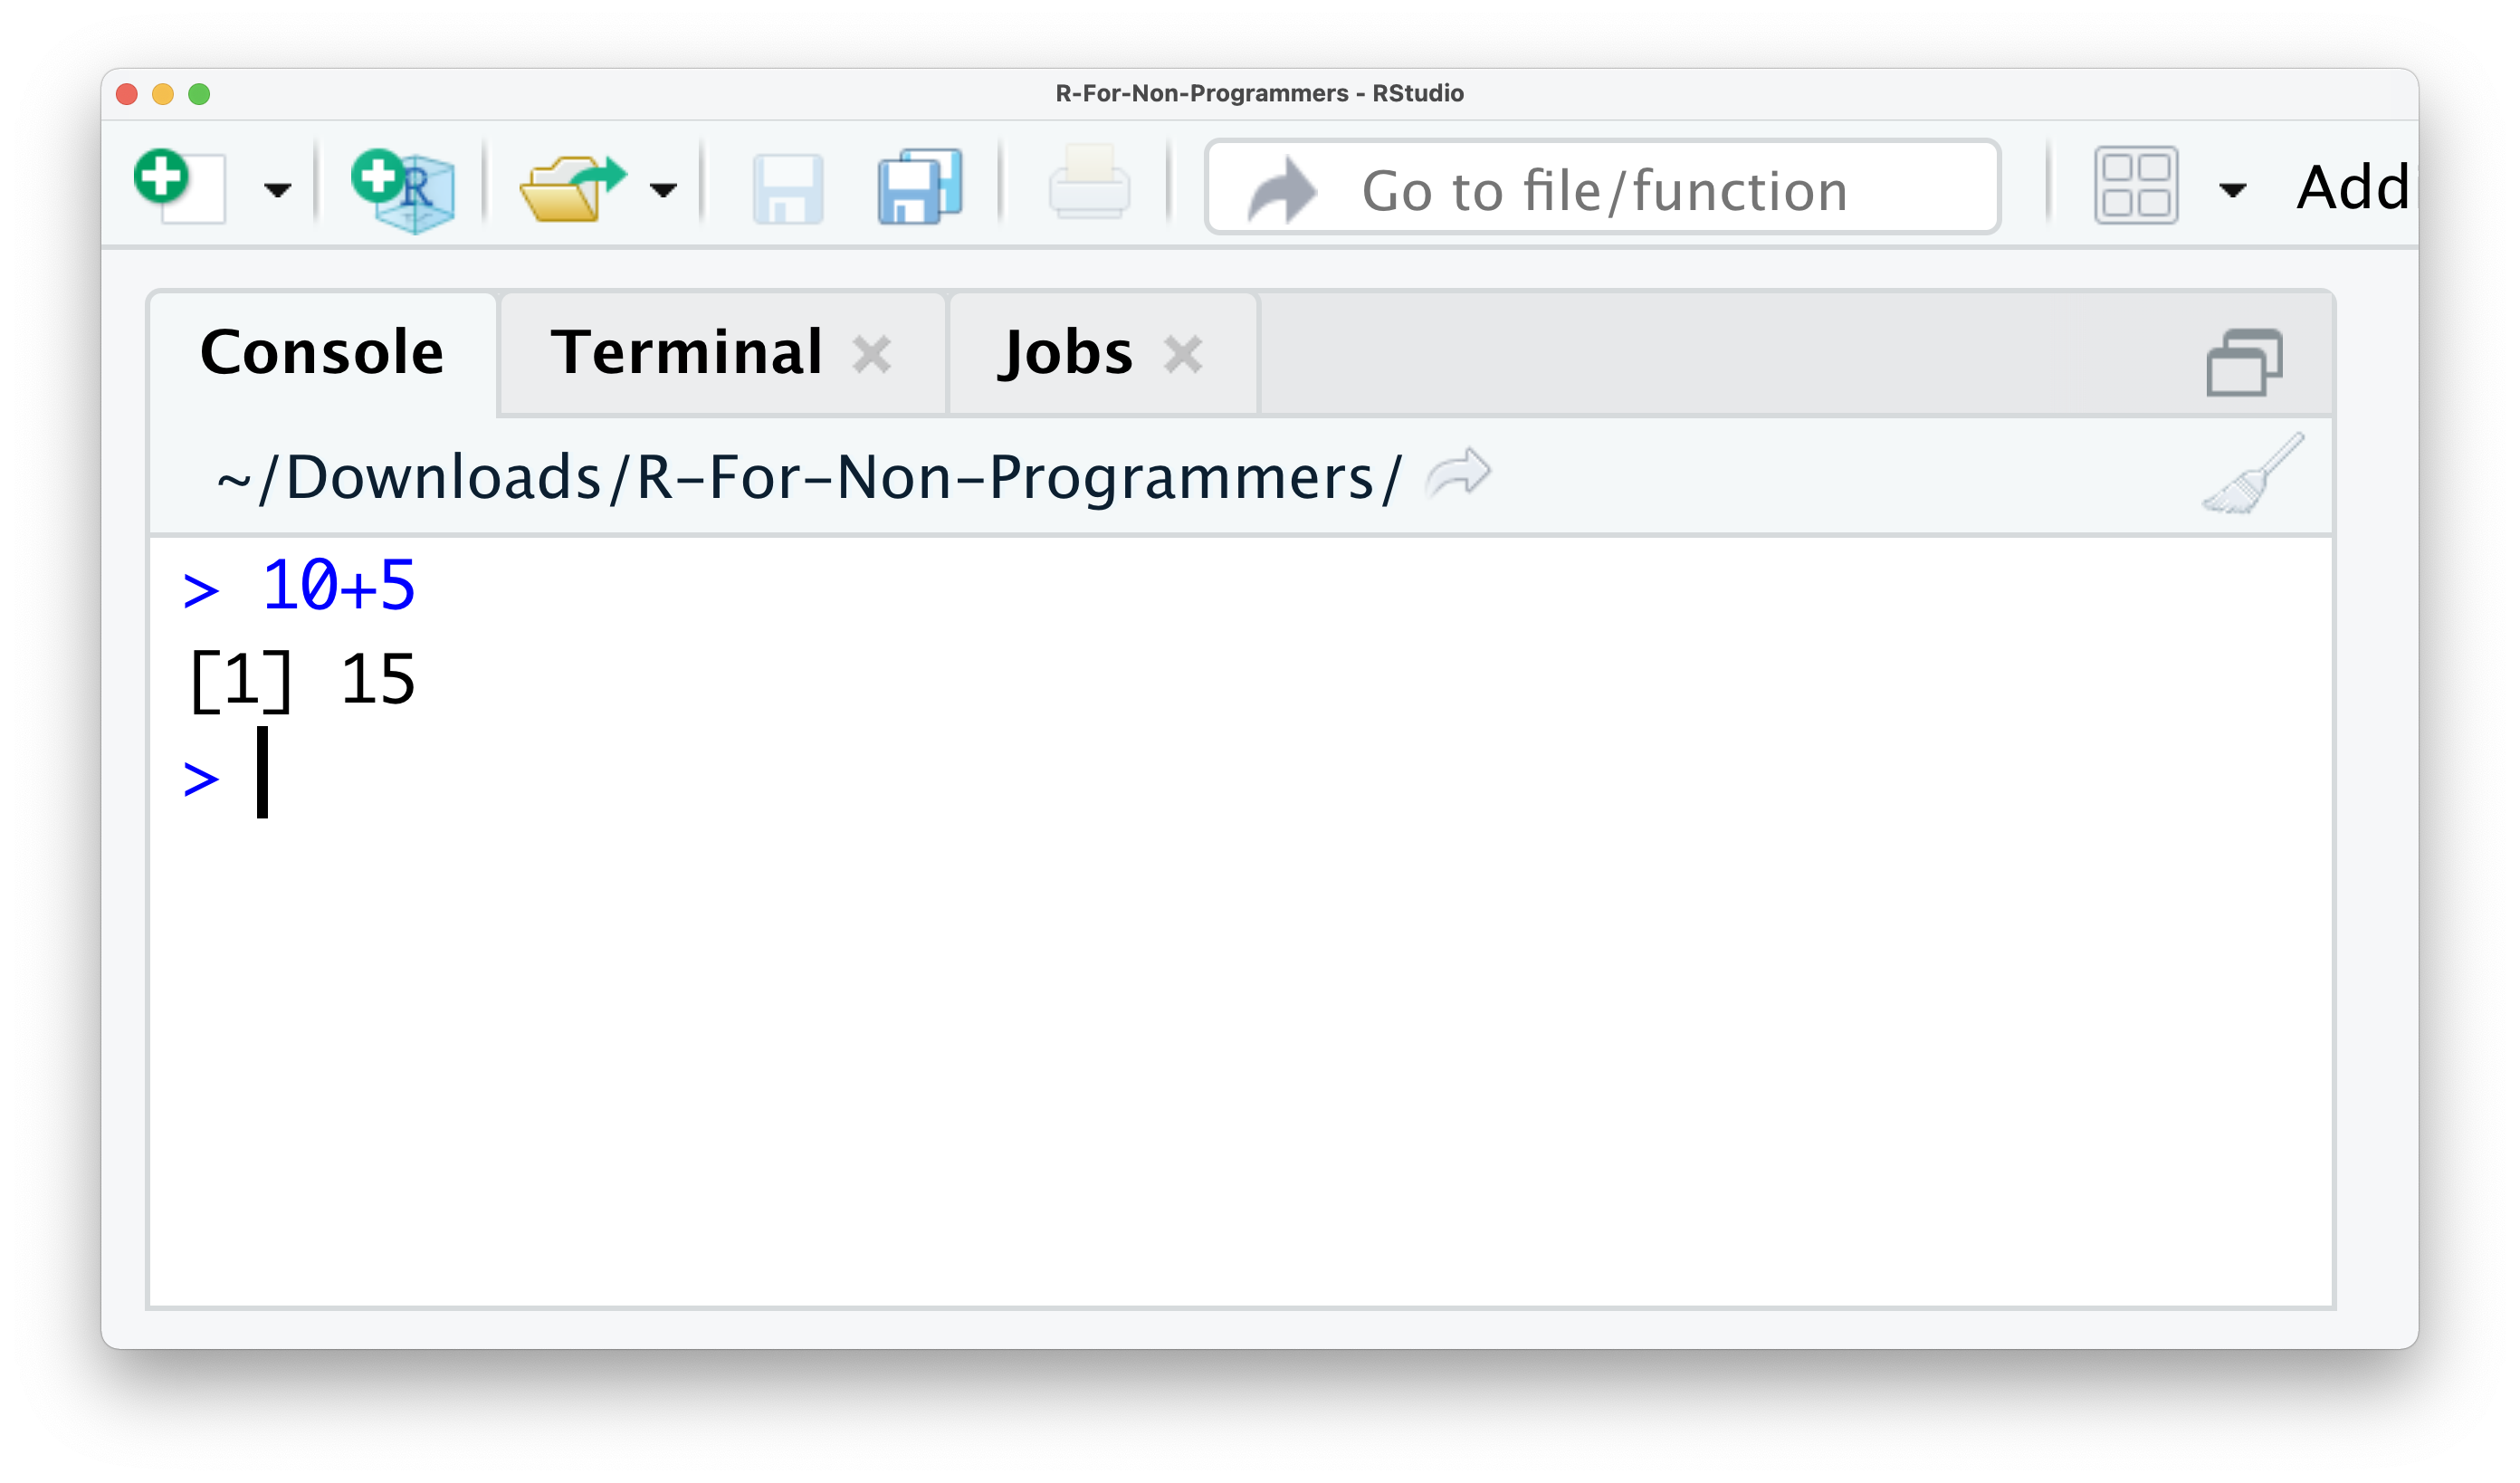
\includegraphics{images/chapter_04_img/02_console_window/console_algebra.png}

You just successfully performed your first successful computation. I know, this is not quite impressive just yet. \emph{R} is undoubtedly more than just a giant calculator.

In the top right of the console, you find a symbol that looks like a broom. This one is quite an important one because it clears your console. Sometimes the console can become very cluttered and difficult to read. If you want to remove whatever you computed, you can click the broom icon and clear the console of all text. I use it so frequently that I strongly recommend learning the keyboard shortcut, which is \texttt{Ctrl+L} on PC and Mac.

\hypertarget{the-source-window}{%
\section{The Source window}\label{the-source-window}}

In the top left, you can find the source window. The term `source' can be understood as any type of file, e.g.~data, programming code, notes, etc. The source panel can fulfil many functions, such as:

\begin{itemize}
\item
  Inspect data in an Excel-like format (LINK TO RELEVANT CHAPTER)
\item
  Open programming code, e.g.~an R Script (LINK TO RELEVANT CHAPTER)
\item
  Open other text-based file formats, e.g.

  \begin{itemize}
  \item
    Plain text (.txt),
  \item
    Markdown (.md),
  \item
    Websites (.html),
  \item
    LaTeX (.tex),
  \item
    BibTex (.bib),
  \end{itemize}
\item
  Edit scripts with code in it,
\item
  Run the analysis you have written.
\end{itemize}

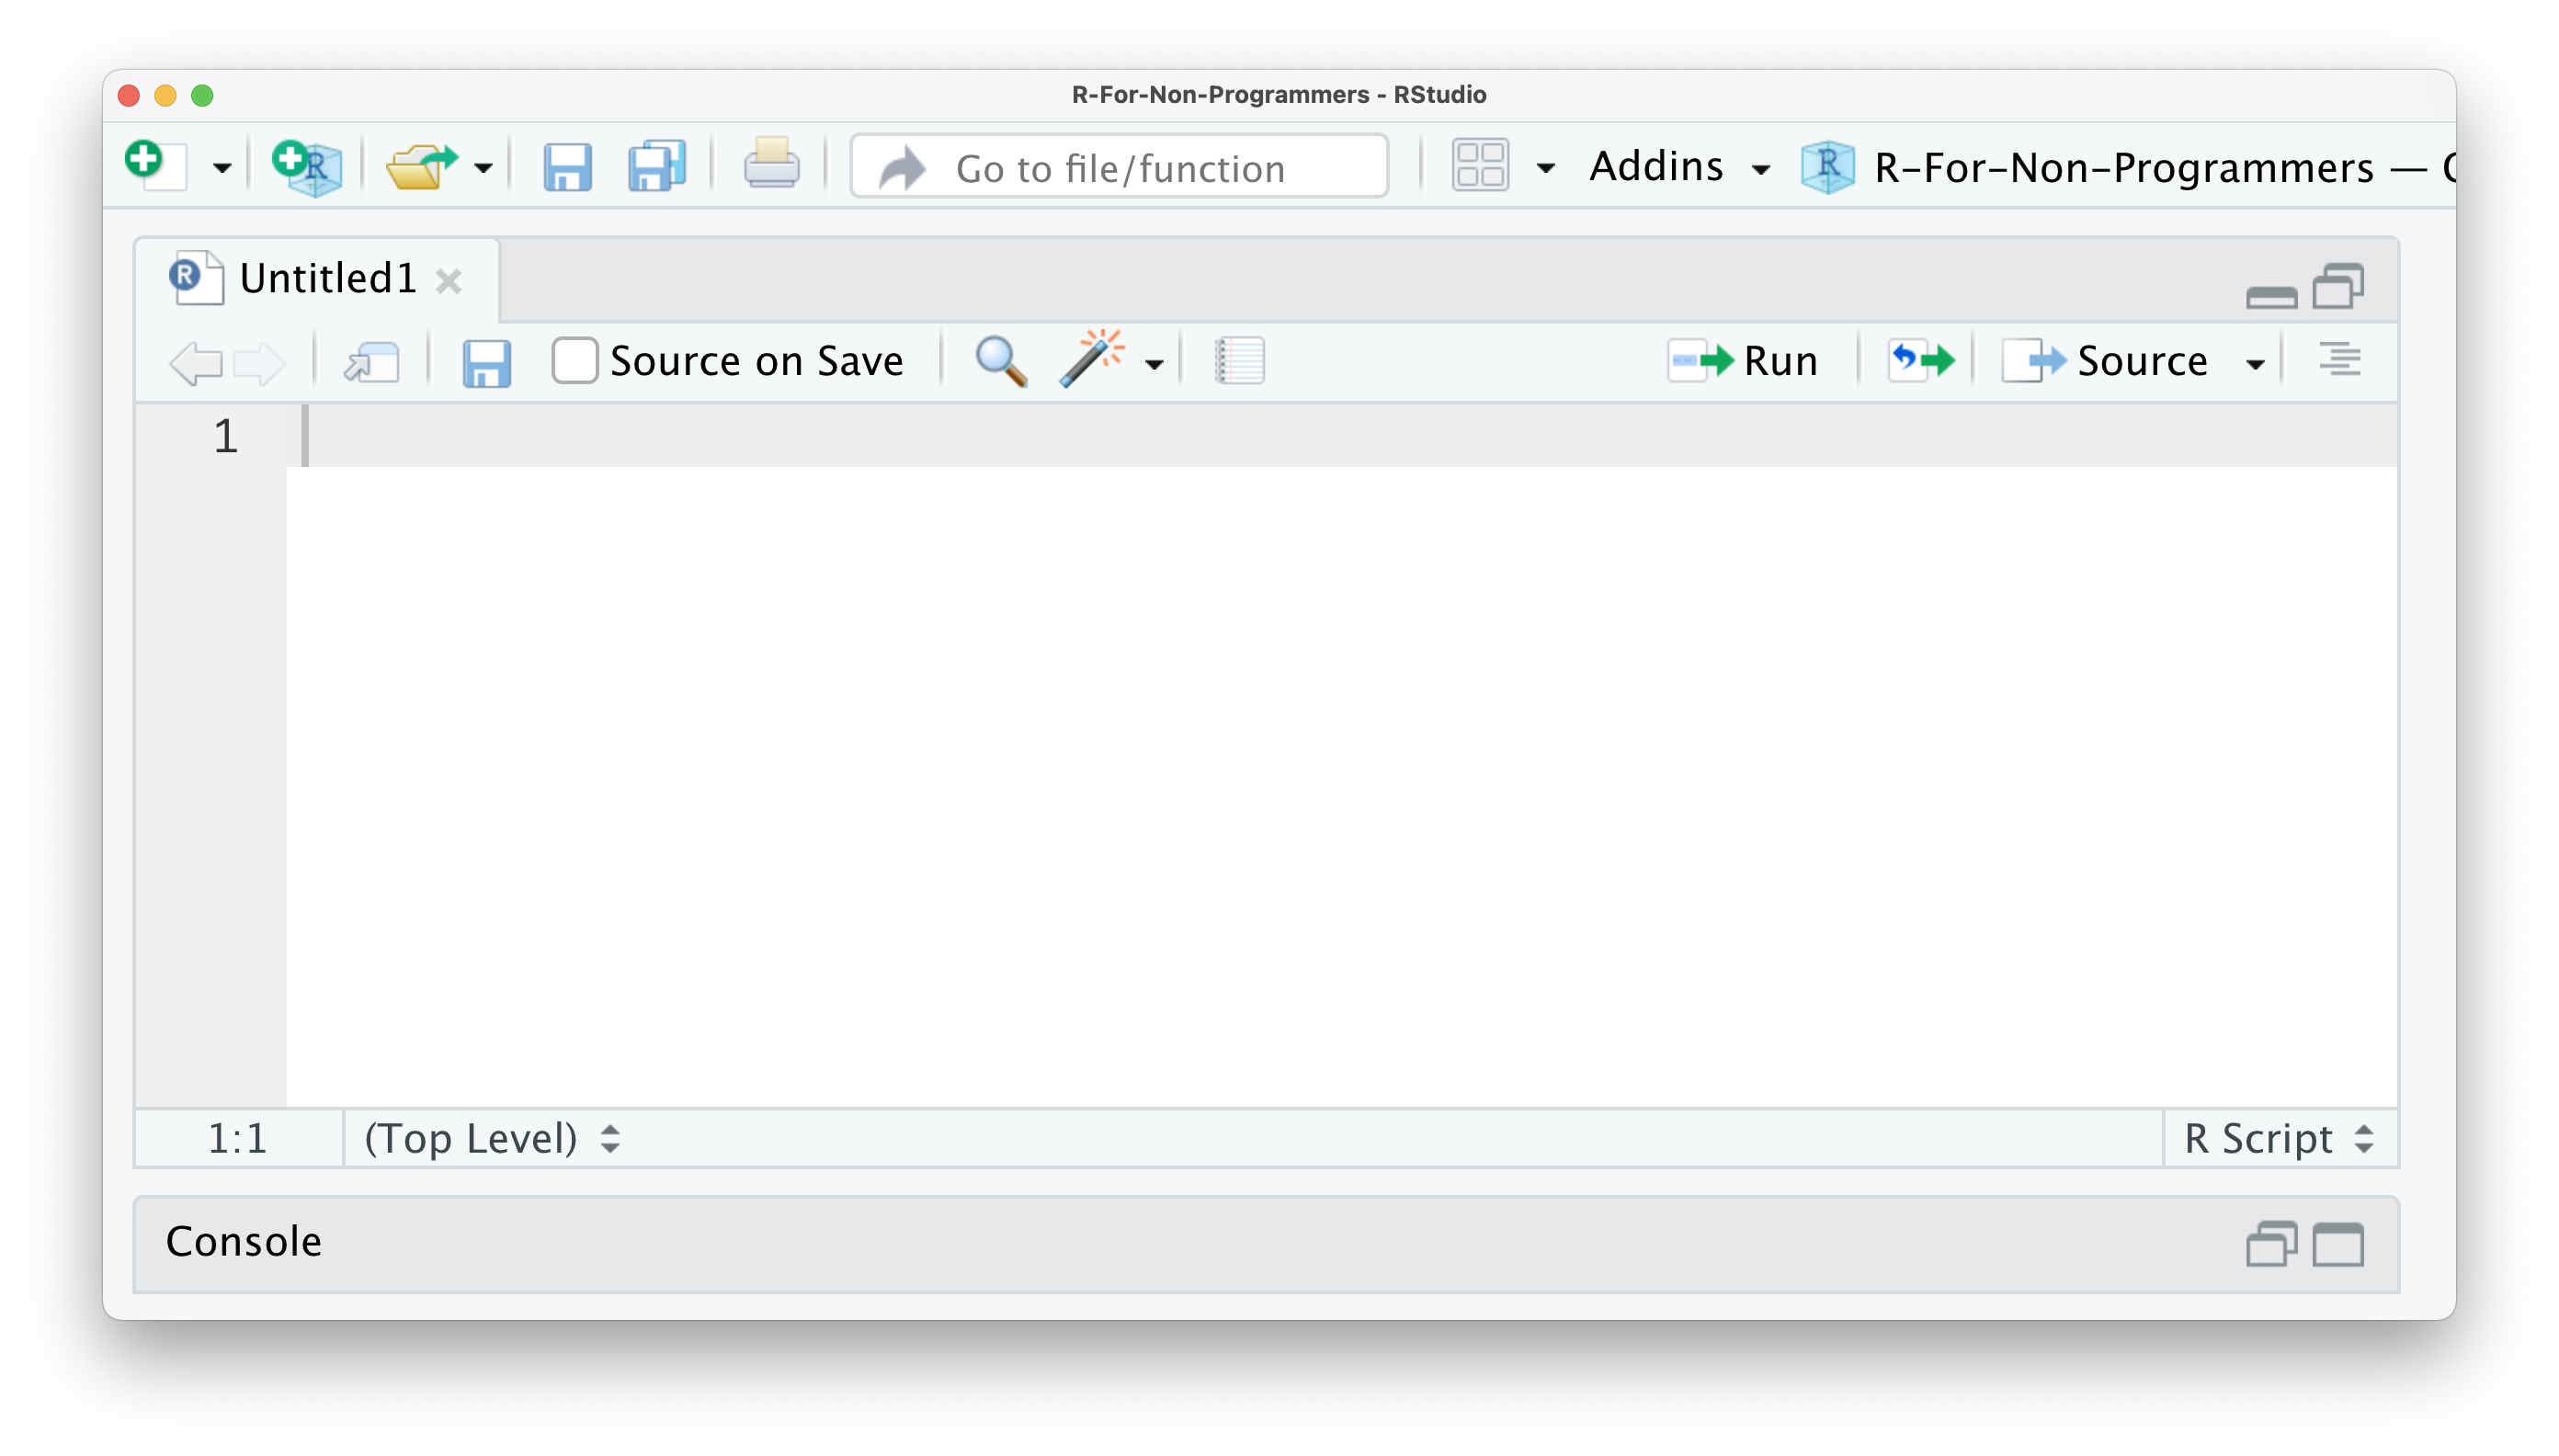
\includegraphics{images/chapter_04_img/03_source_window/01_rstudio_source.png}

In other words, the source window will show you whatever file you are interested in, as long as RStudio can read it - and no, Microsoft Office Documents are not supported. Another limitation of the source window is that it can only show text-based files. So opening images, etc. would not work.

\hypertarget{the-environment-history-connections-tutorial-window}{%
\section{The Environment / History / Connections / Tutorial window}\label{the-environment-history-connections-tutorial-window}}

The window in the top right shows multiples panes. The first pane is called \emph{Environment} and shows you objects which are available for computation. One of the first objects you will create is your dataset because, without data, we cannot perform any analysis. Thus, one object might be your data. Another object could be a plot showing the number of male and female participants in your study. To find out how to create objects yourself, you can take a glimpse at (INSERT CHAPTER X). Besides datasets and plots, you will also find other objects here, e.g.~lists, vectors and functions you created yourself. Don't worry if none of these words makes sense at this point. We will cover each of them in the upcoming chapters. For now, remember this is a place where you can find different objects you created.

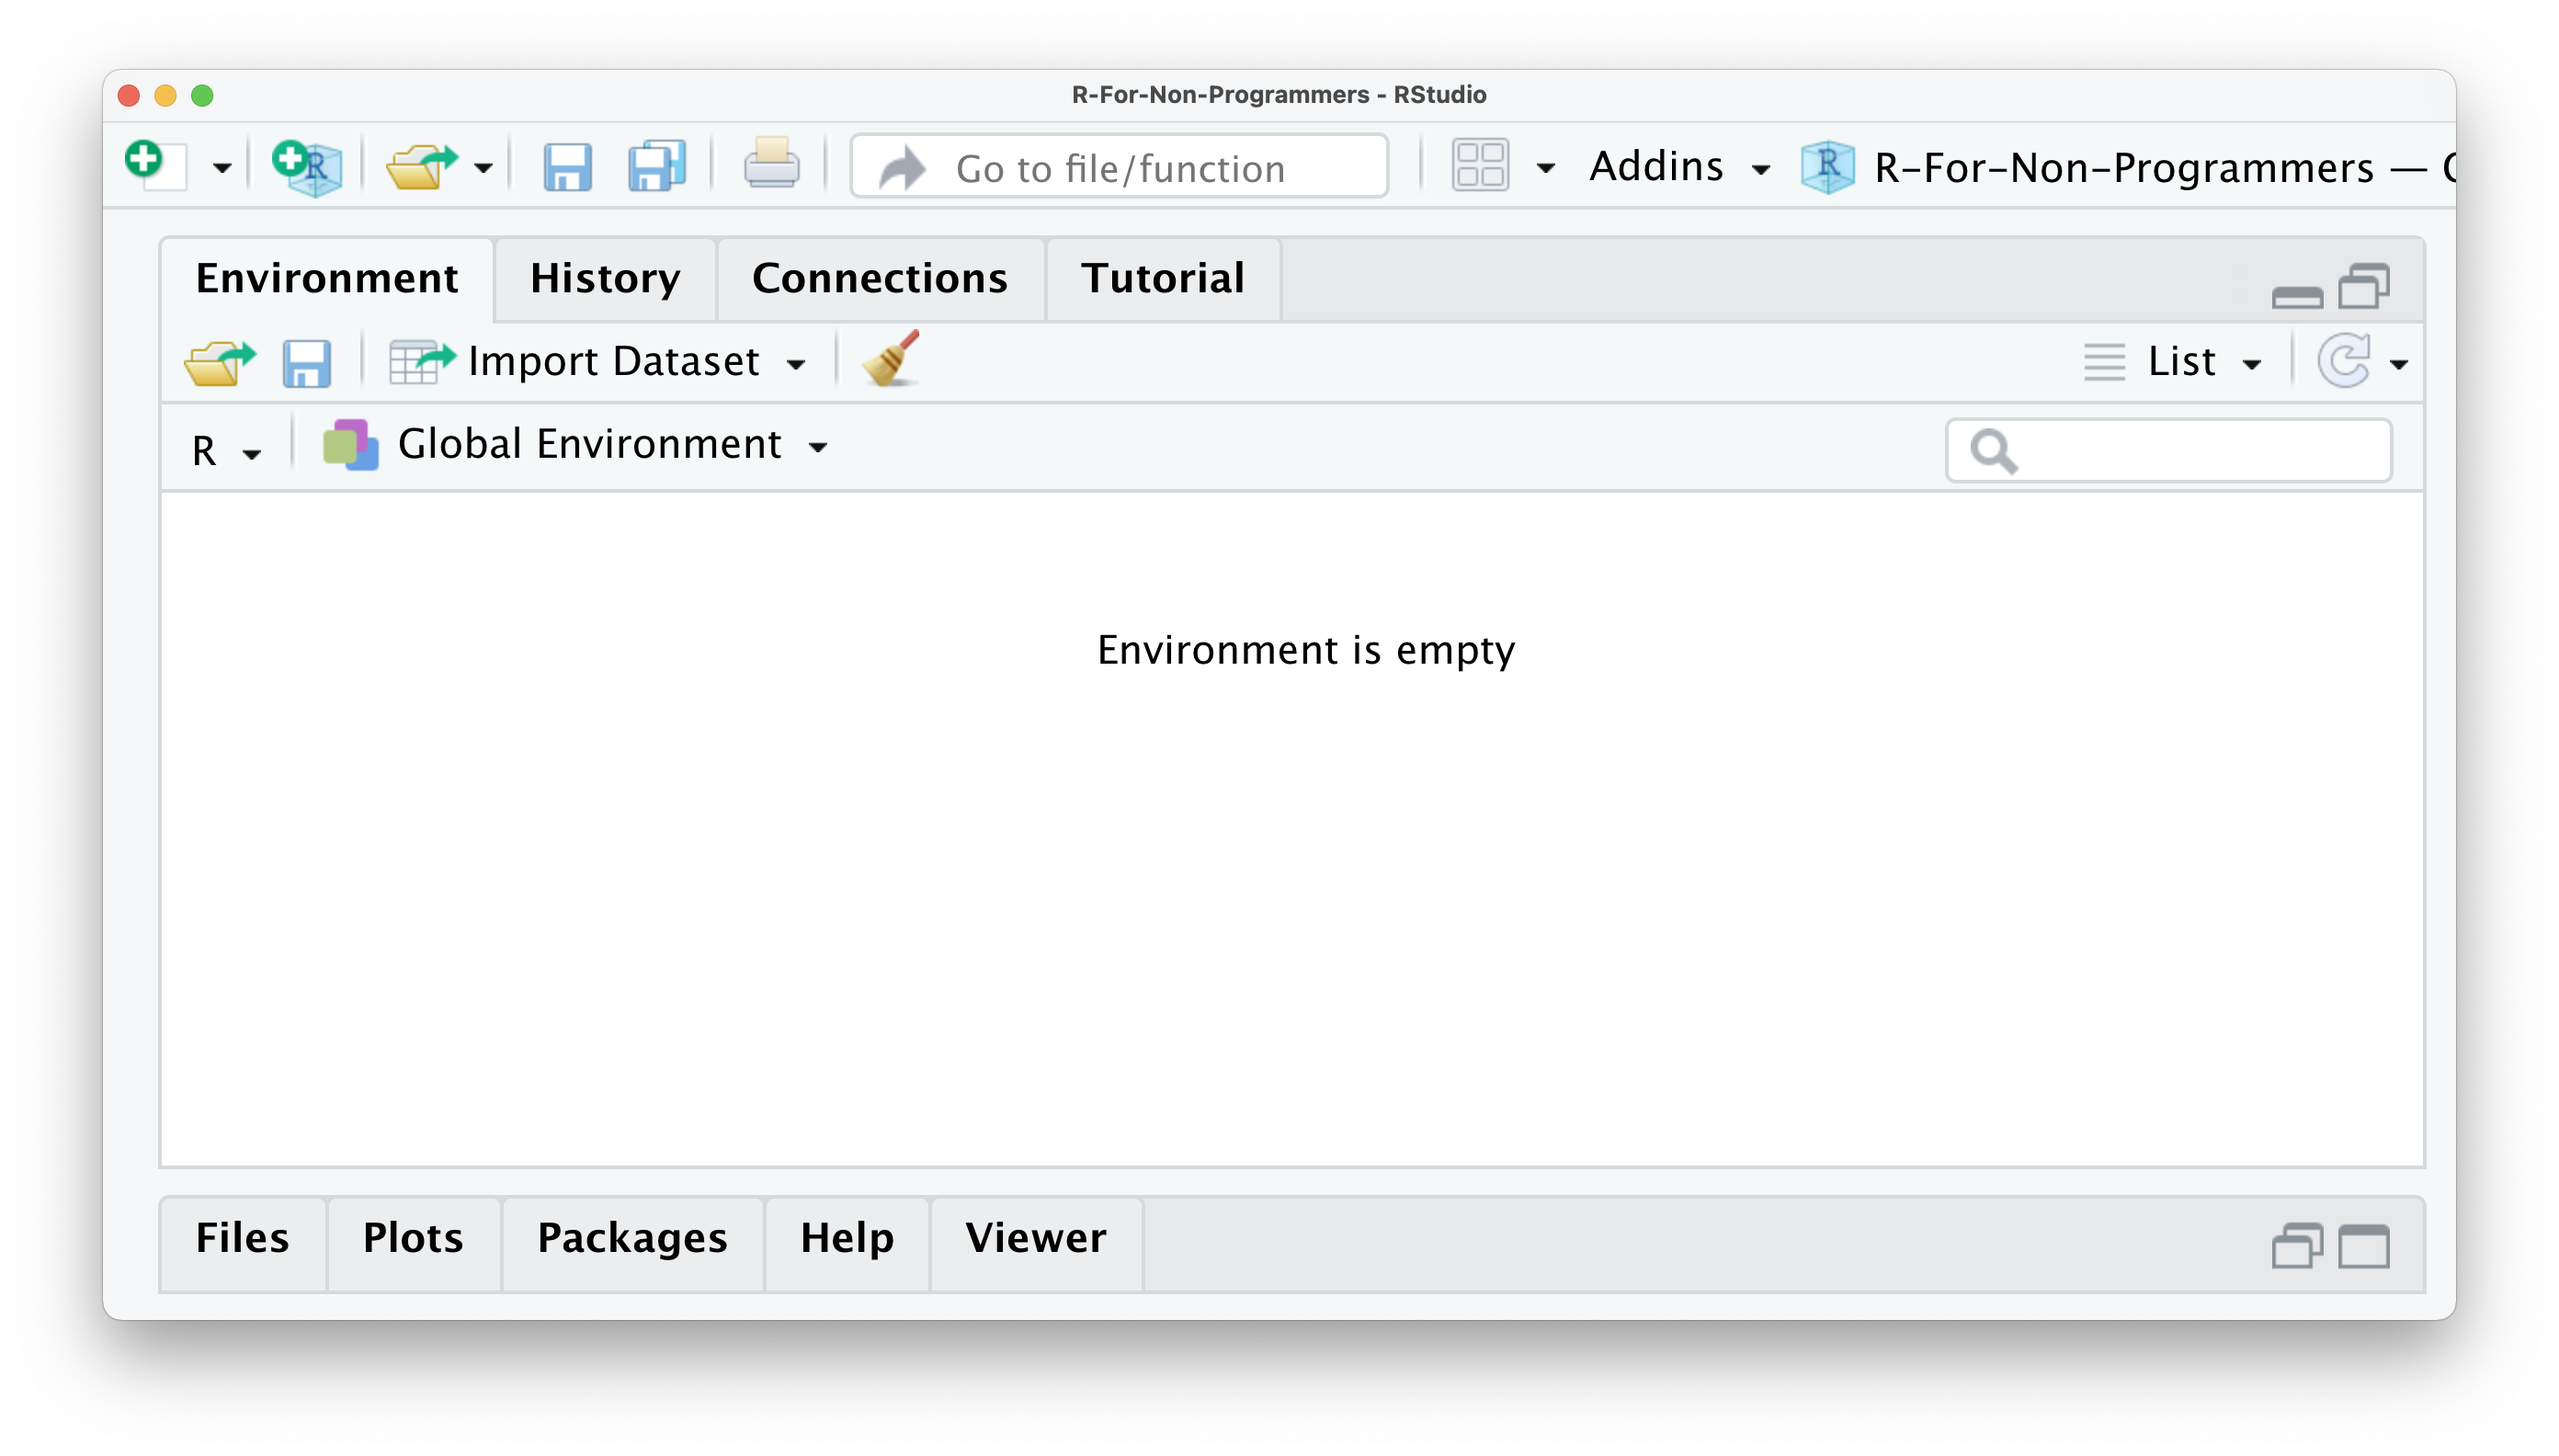
\includegraphics{images/chapter_04_img/04_environment_history_etc/01_rstudio_environment.png}

The \emph{History} pane is very easy to understand. Whatever computation you run in the Console will be stored. So you can go back and see what you coded and rerun that code. Remember the example from above where we computed the sum of \texttt{10+5}? This computation is stored in the history of RStudio, and you can rerun it by clicking on \texttt{10+5} in the history pane and then click on \texttt{To\ Console}. This will insert \texttt{10+5} back into the Console, and we can hit \texttt{Return\ ↵} to retrieve the result. You also have the option to copy the code into an existing or new R Script by clicking on \texttt{To\ Source}. By doing this, you can save this computation on your computer and reuse it later. Finally, if you would like to store your history, you can do so by clicking on the \texttt{floppy\ disk\ symbol}. There are two more buttons in this pane, one allows you to delete individual entries in the history, and the last one, a \texttt{broom}, clears the entire history (irrevocably).

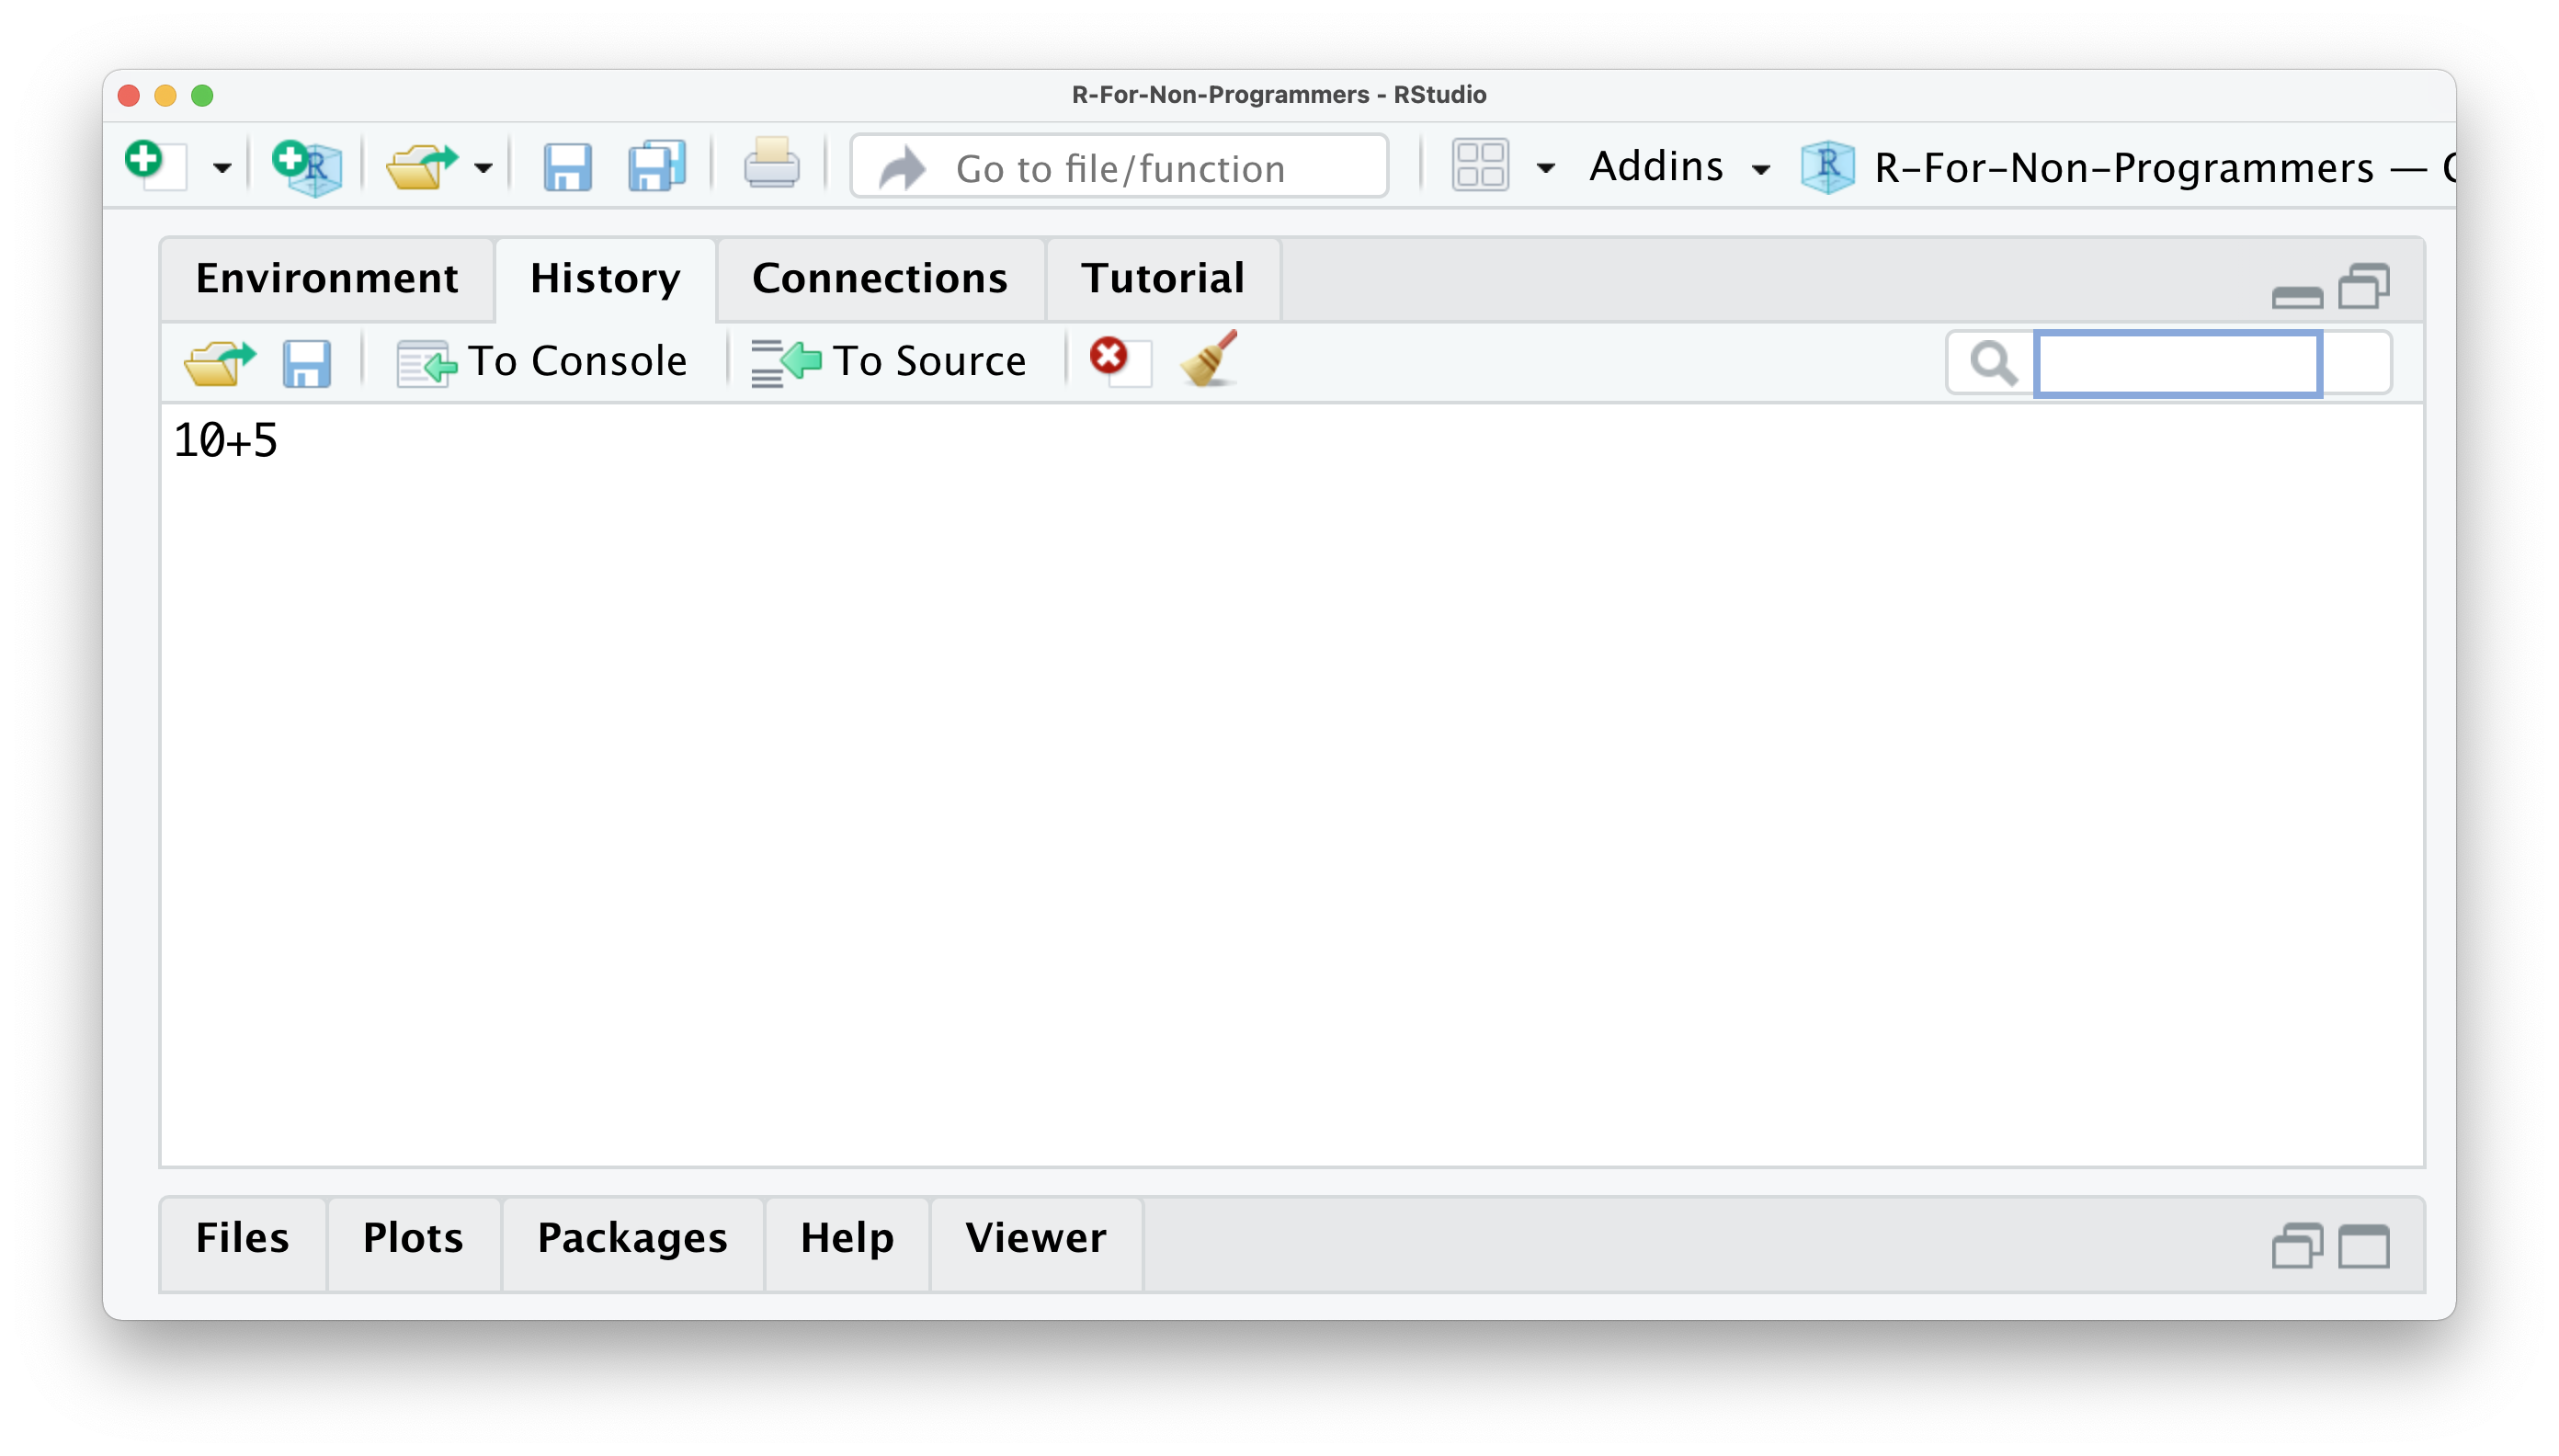
\includegraphics{images/chapter_04_img/04_environment_history_etc/02_rstudio_history.png}

The pane \emph{Connections} allows you to tab into external databases directly. This can come in handy when you work collaboratively on the same data or want to work with extensive datasets without having to download them. However, for an introduction to R, we will not use this feature of RStudio for now.

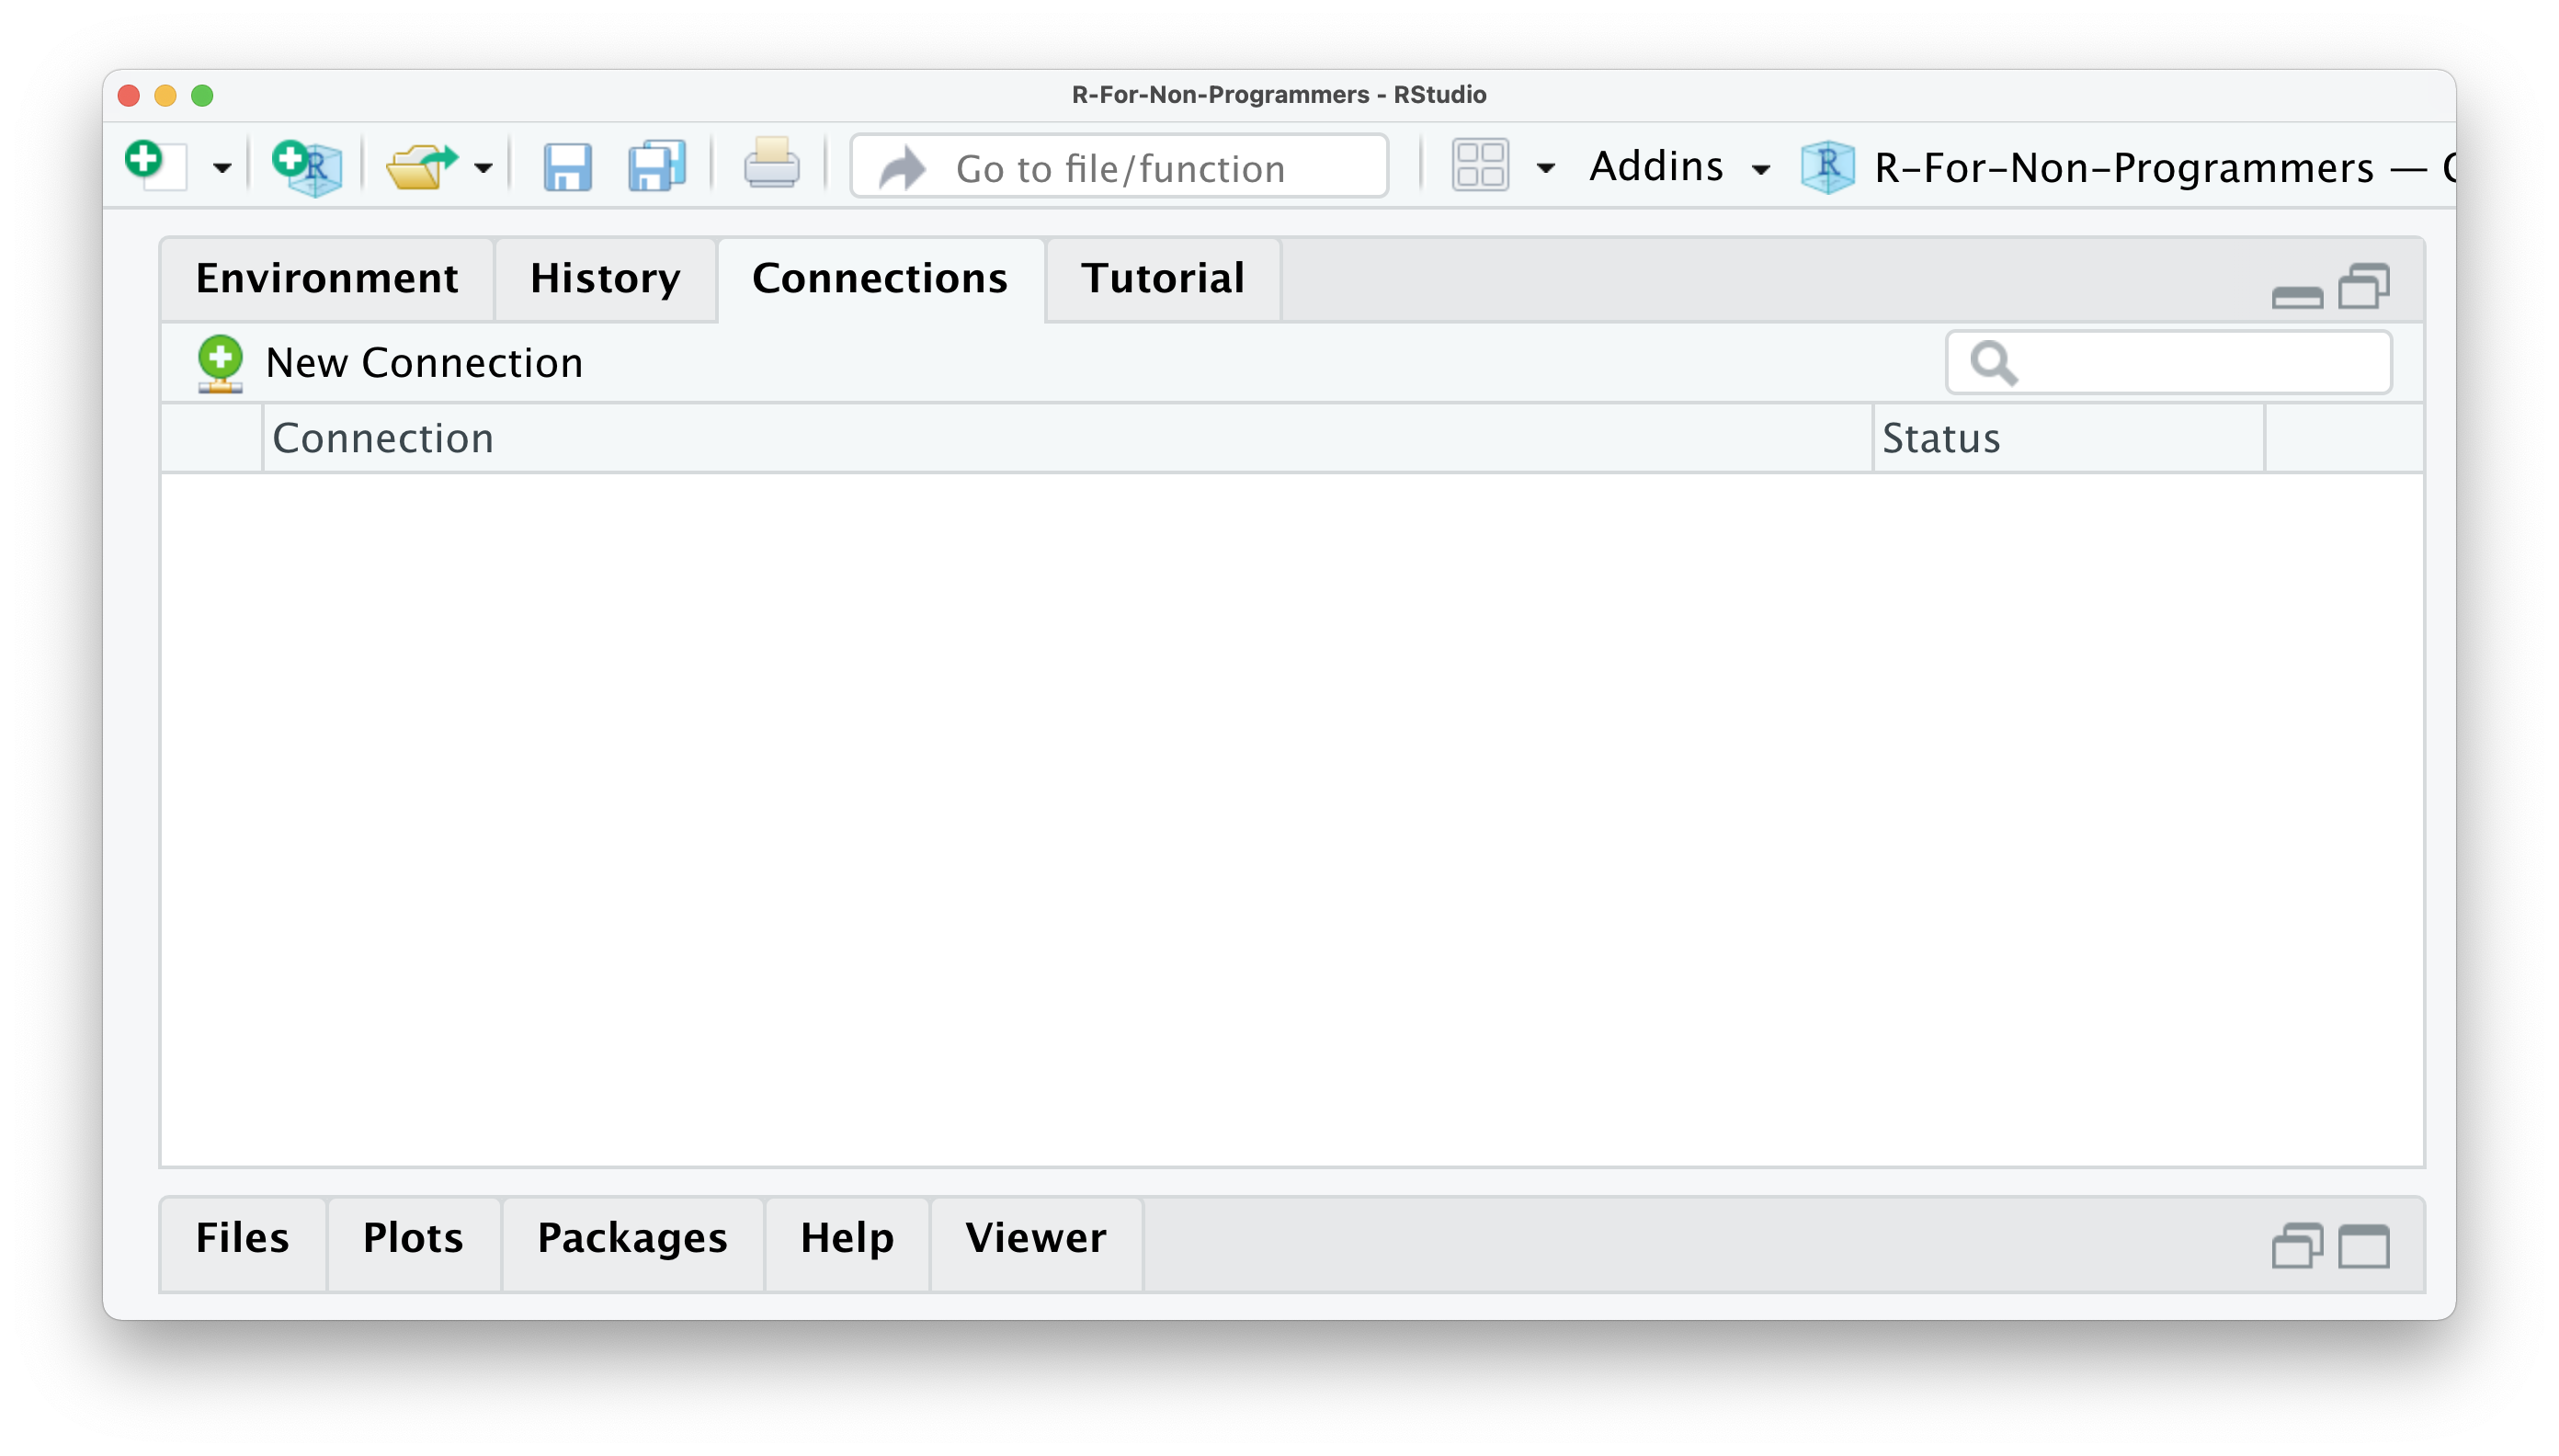
\includegraphics{images/chapter_04_img/04_environment_history_etc/03_rstudio_connections.png}

The last pane is called \emph{Tutorial}. Here you can find additional materials to learn \emph{R} and RStudio. If you search for more great content to learn R, this serves as a great starting point.

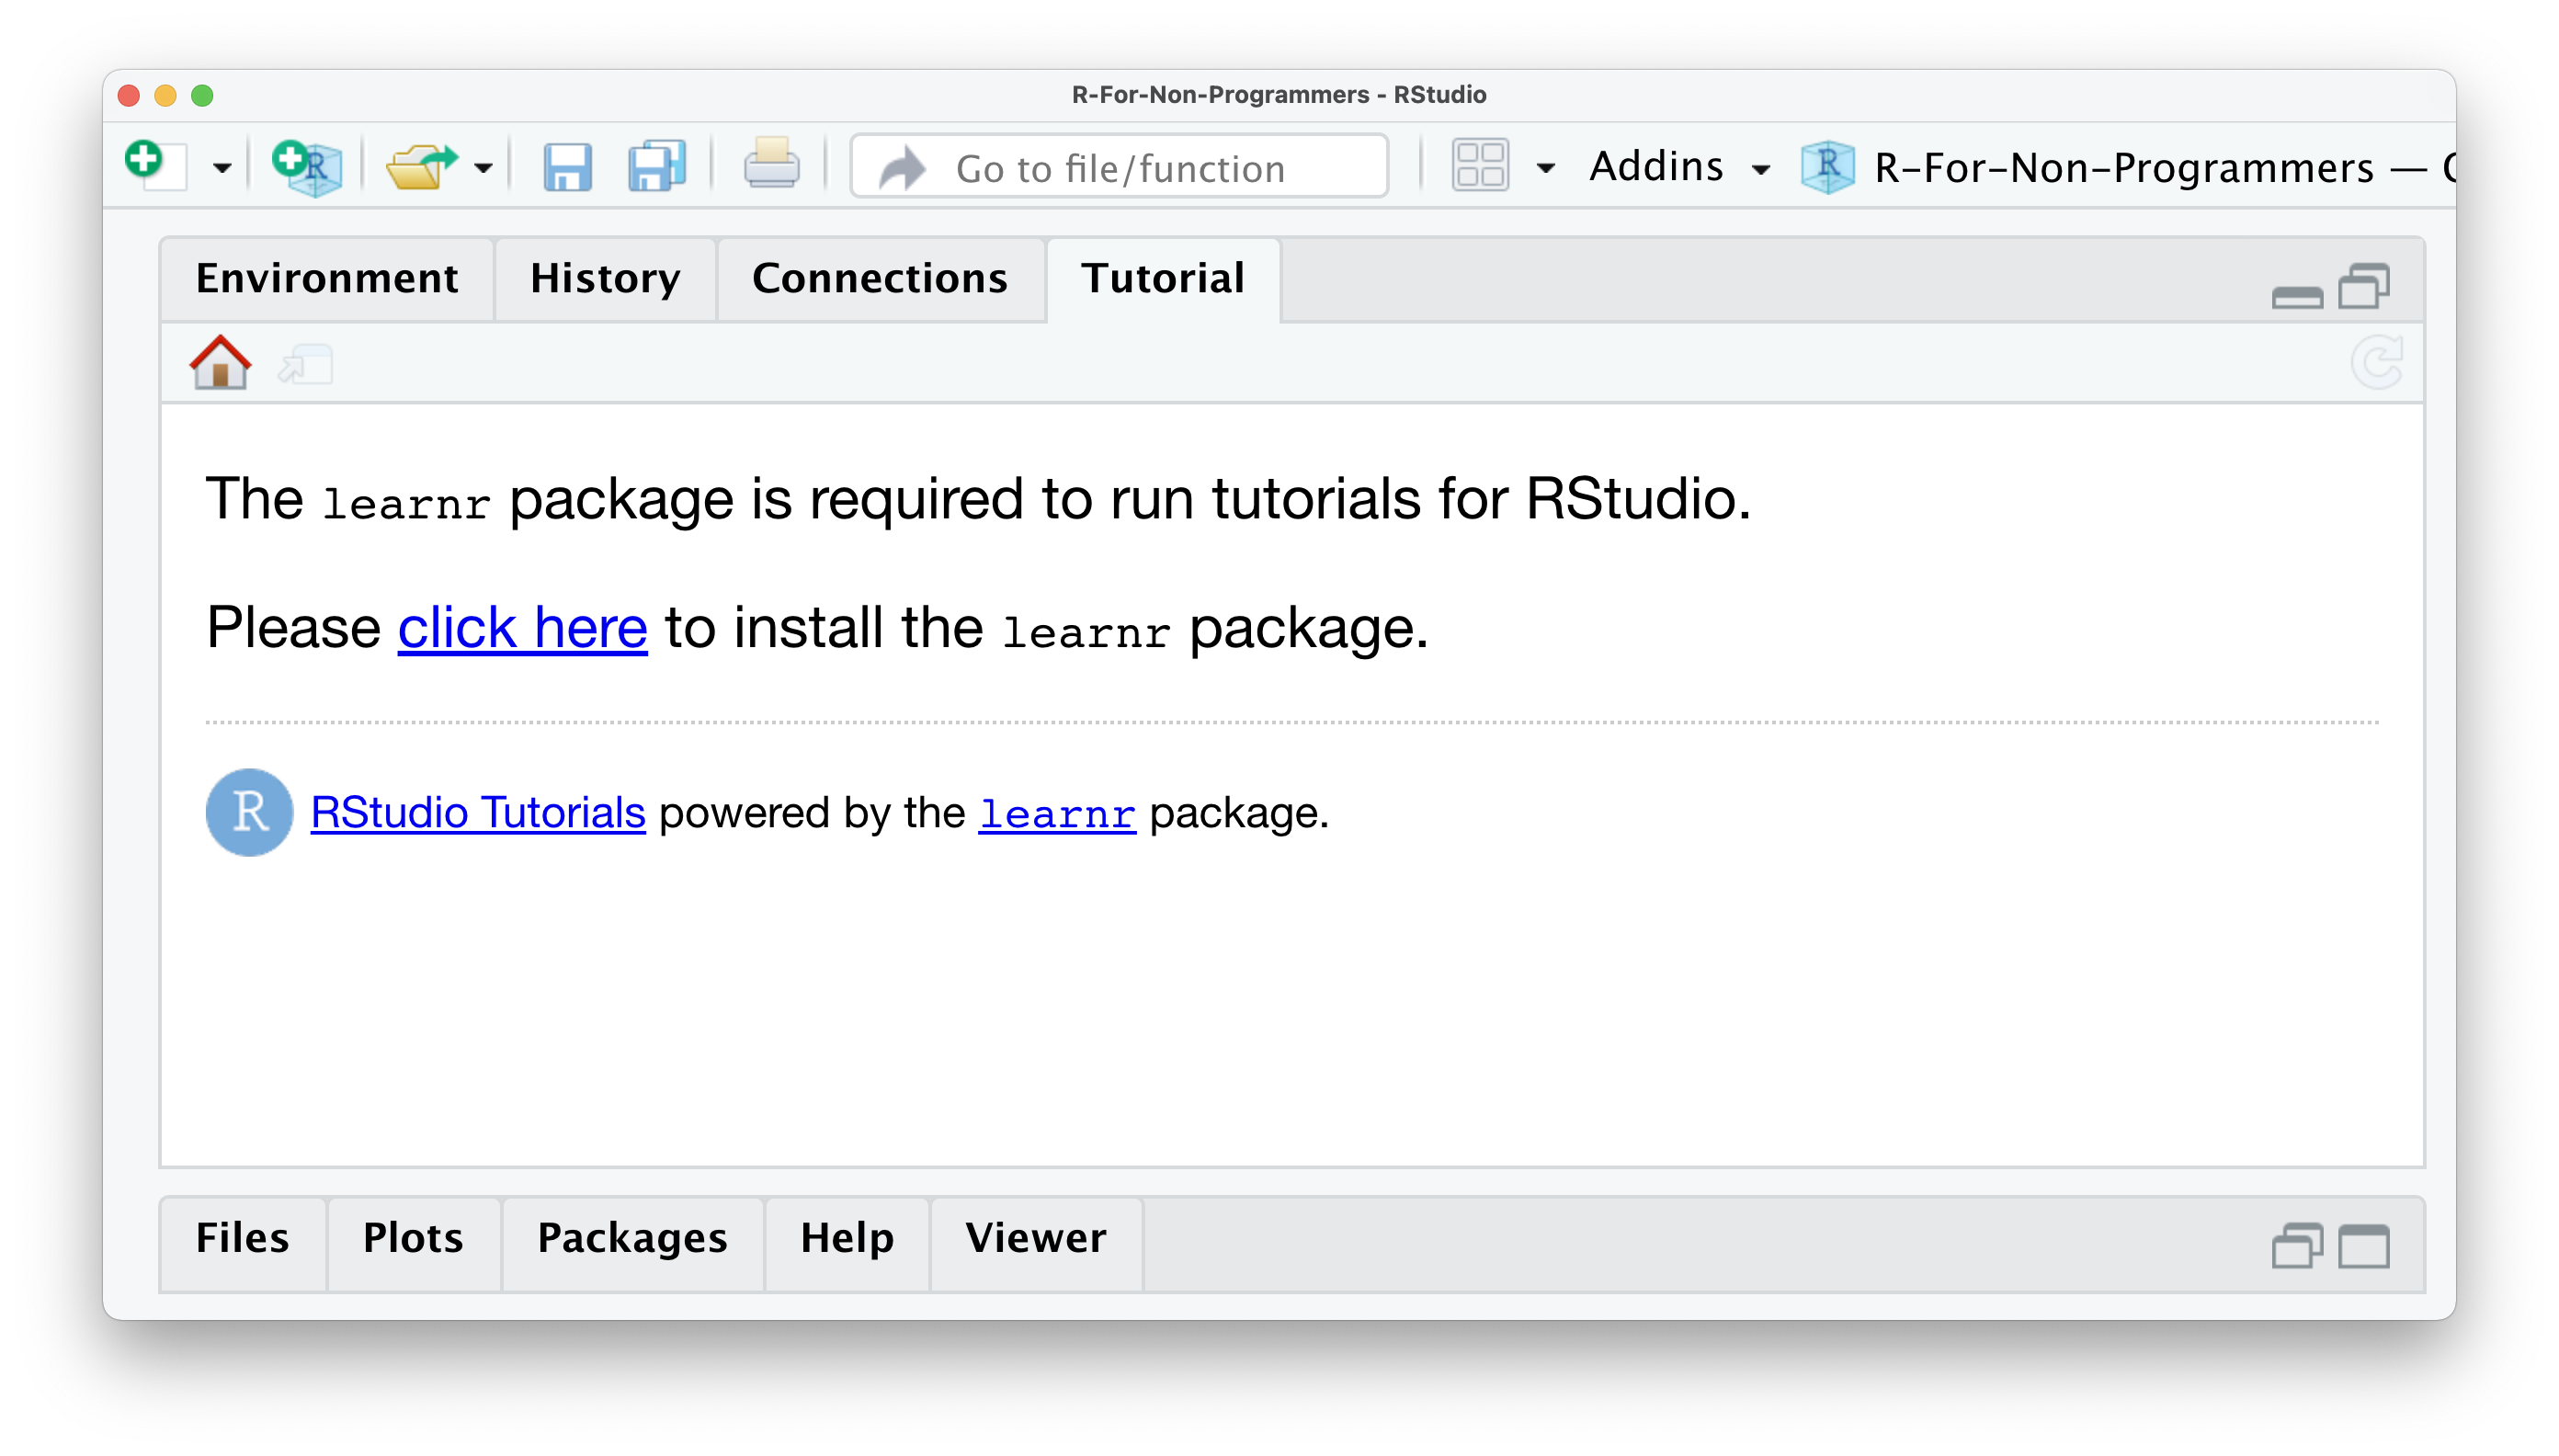
\includegraphics{images/chapter_04_img/04_environment_history_etc/04_rstudio_tutorial.png}

\hypertarget{the-files-plots-packages-help-viewer-window}{%
\section{The Files / Plots / Packages / Help / Viewer window}\label{the-files-plots-packages-help-viewer-window}}

The last window consists of five essential panes. The first one is the \emph{Files} pane. As the name indicates, it lists all the files and folders in your root directory. A root directory is the default directory where RStudio saves your files, for example, your analysis. However, you can easily change this directory to something else (see also CHAPTER X) or use R Project files (see CHAPTER X) to carry out your research. Thus, the \emph{Files} pane is an easy way to load data into RStudio and create folders to keep your research project well organised.

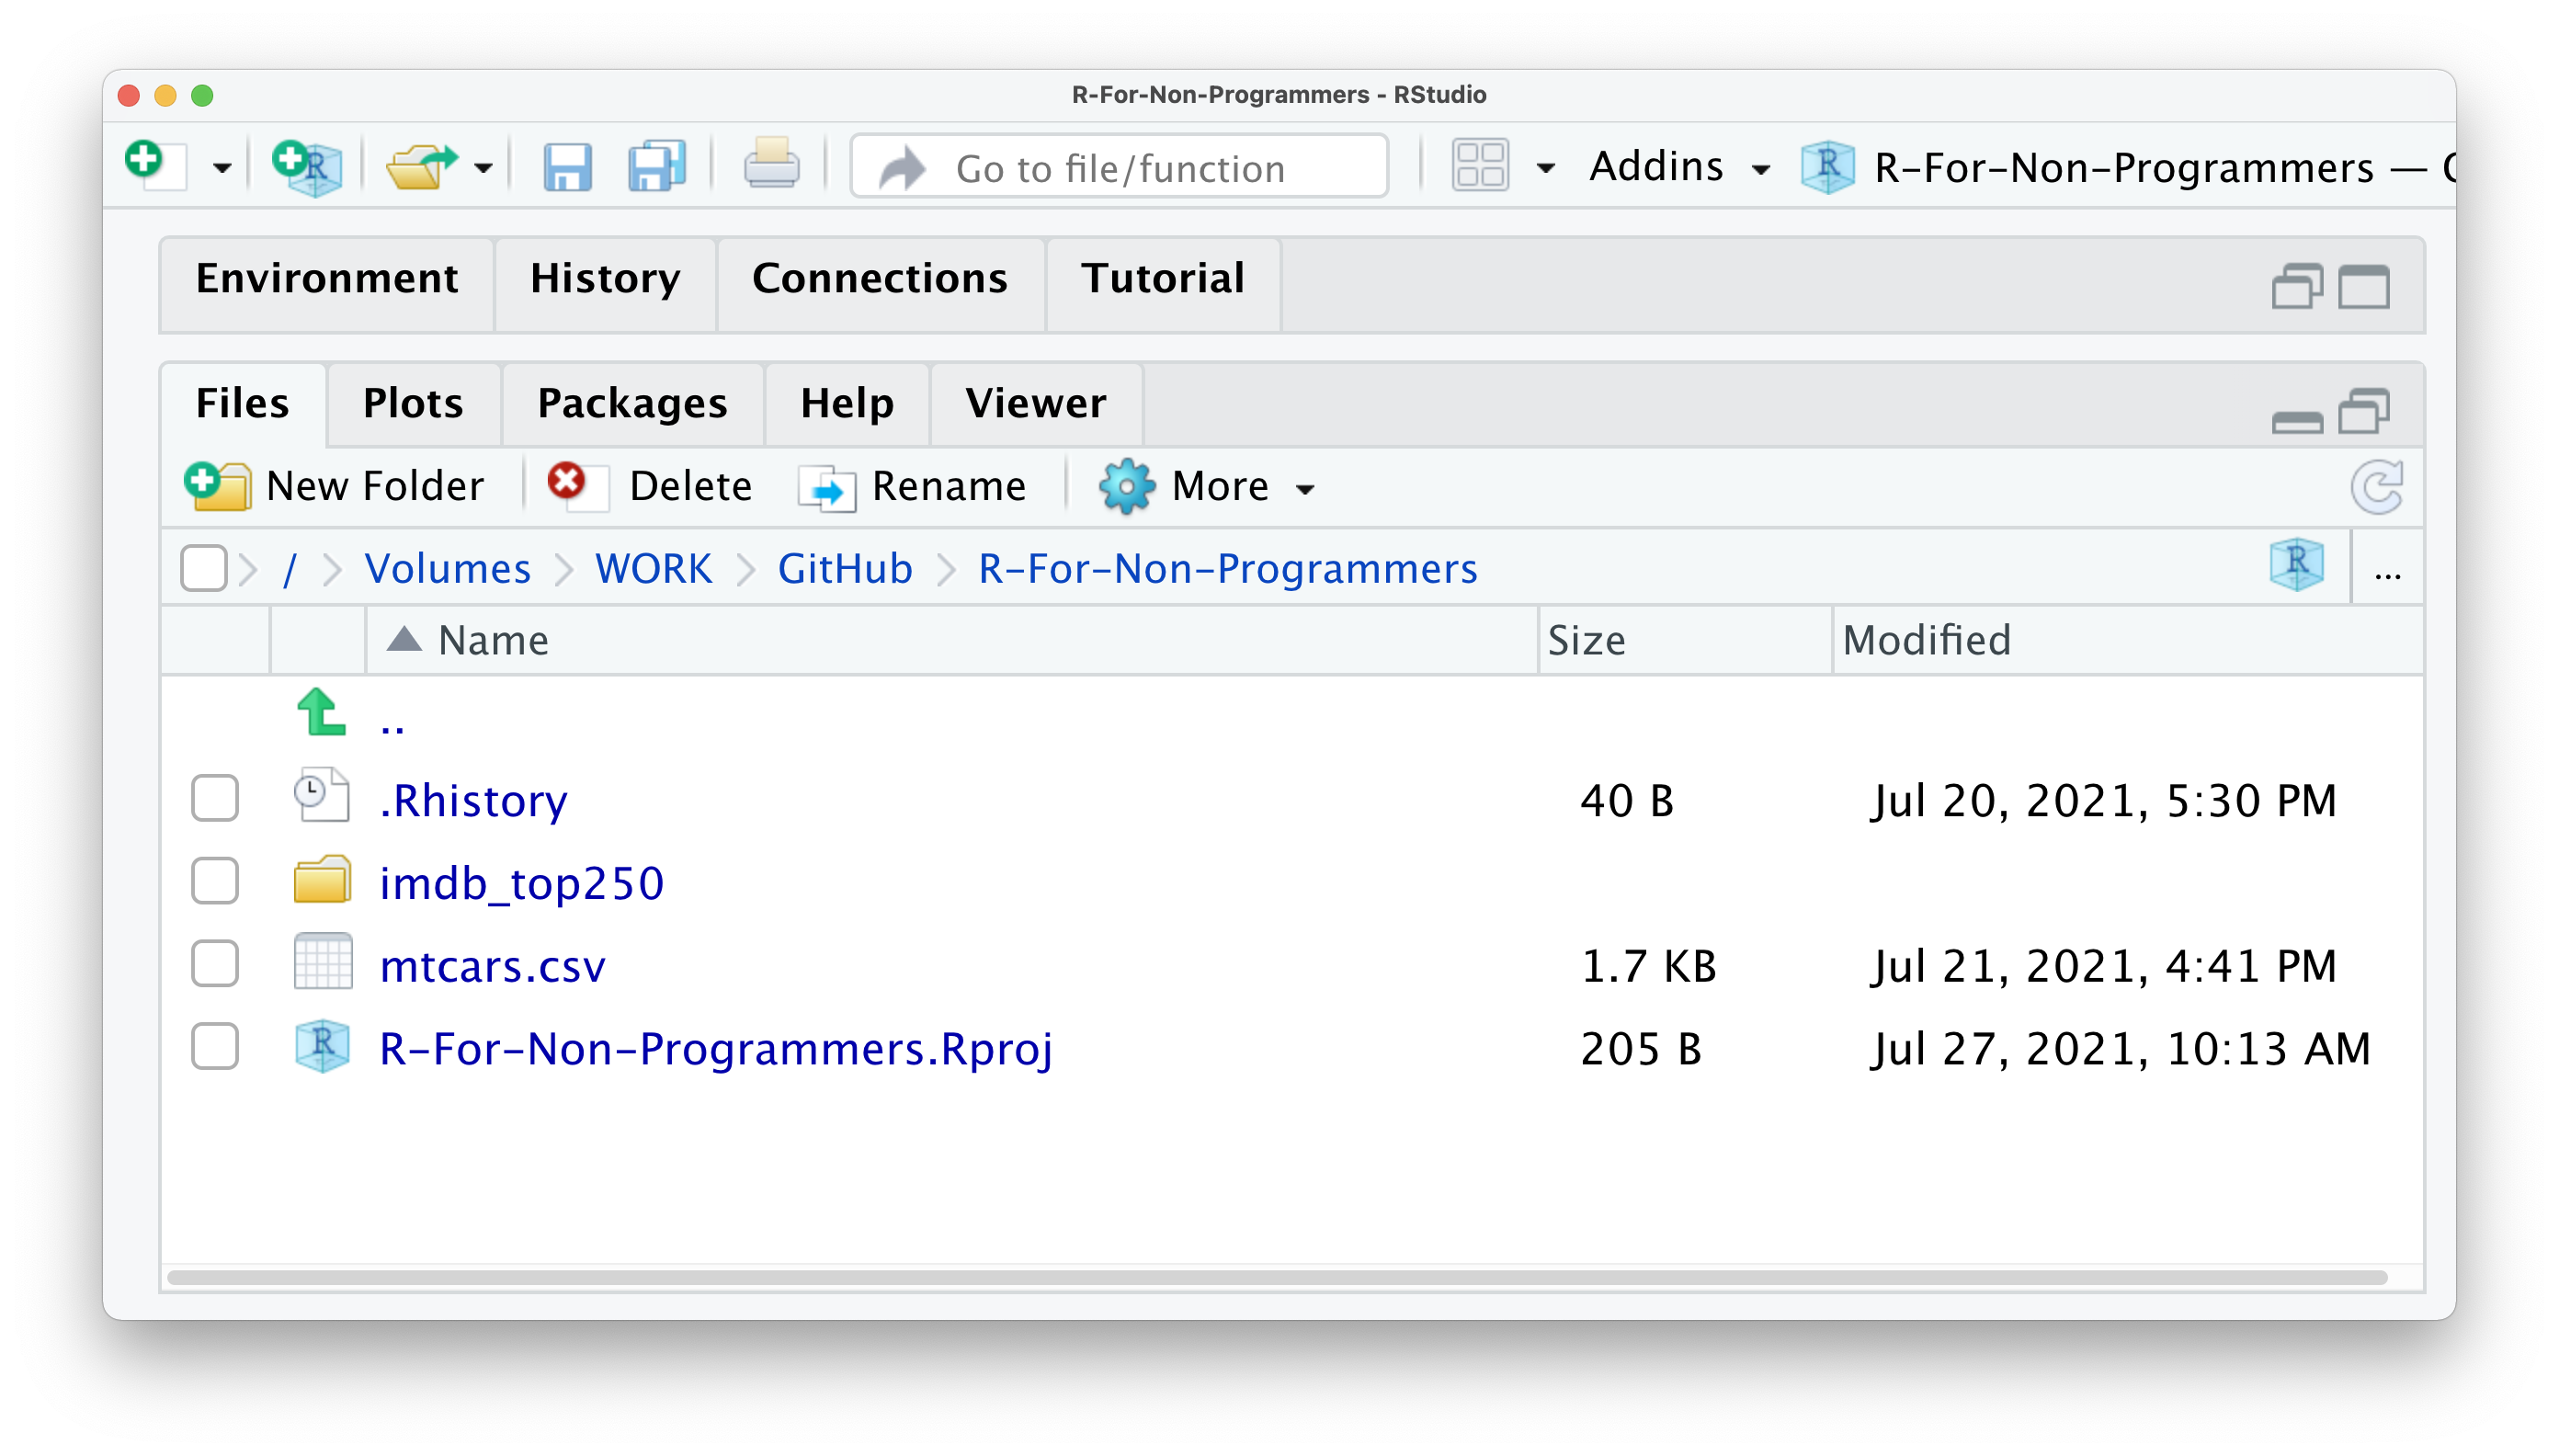
\includegraphics{images/chapter_04_img/05_files_plots_etc/01_rstudio_files.png}

Since the Console cannot reproduce data visualisations, RStudio offers a way to do this very easily. It is through the Plots pane. This pane is exclusively designed to show you any plots you have created using R. Here is a simple example that you can try. Type into your console \texttt{boxplot(mtcars\$hp)}.

\begin{Shaded}
\begin{Highlighting}[]
\CommentTok{\# Here we create a nice boxplot using a dataset called \textquotesingle{}mtcars\textquotesingle{}}
\FunctionTok{boxplot}\NormalTok{(mtcars}\SpecialCharTok{$}\NormalTok{hp)}
\end{Highlighting}
\end{Shaded}

\begin{center}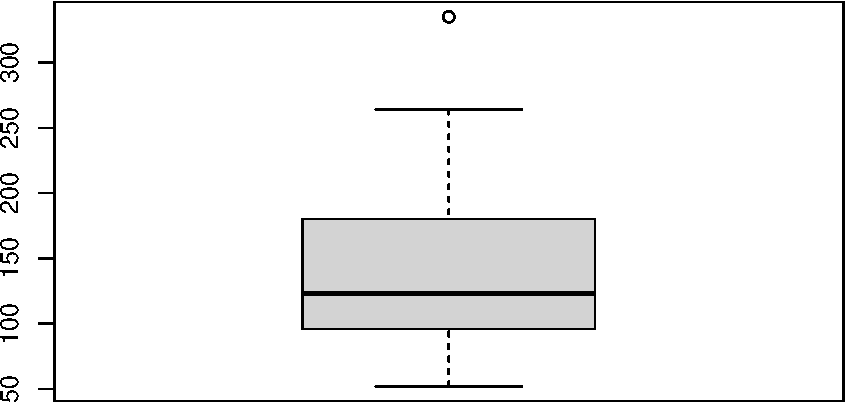
\includegraphics{r_for_non_programmers_files/figure-latex/Simple boxplot-1} \end{center}

Although this is a short piece of coding, it performs quite a lot of steps:

\begin{itemize}
\item
  it uses a function called \texttt{boxplot()} to draw a boxplot of
\item
  a variable called \texttt{hp} (for horsepower), which is located in
\item
  a dataset named \texttt{mtcars},
\item
  and it renders the graph in your \emph{Plots} pane
\end{itemize}

This is how the plot should look like in your RStudio \emph{Plots} pane.

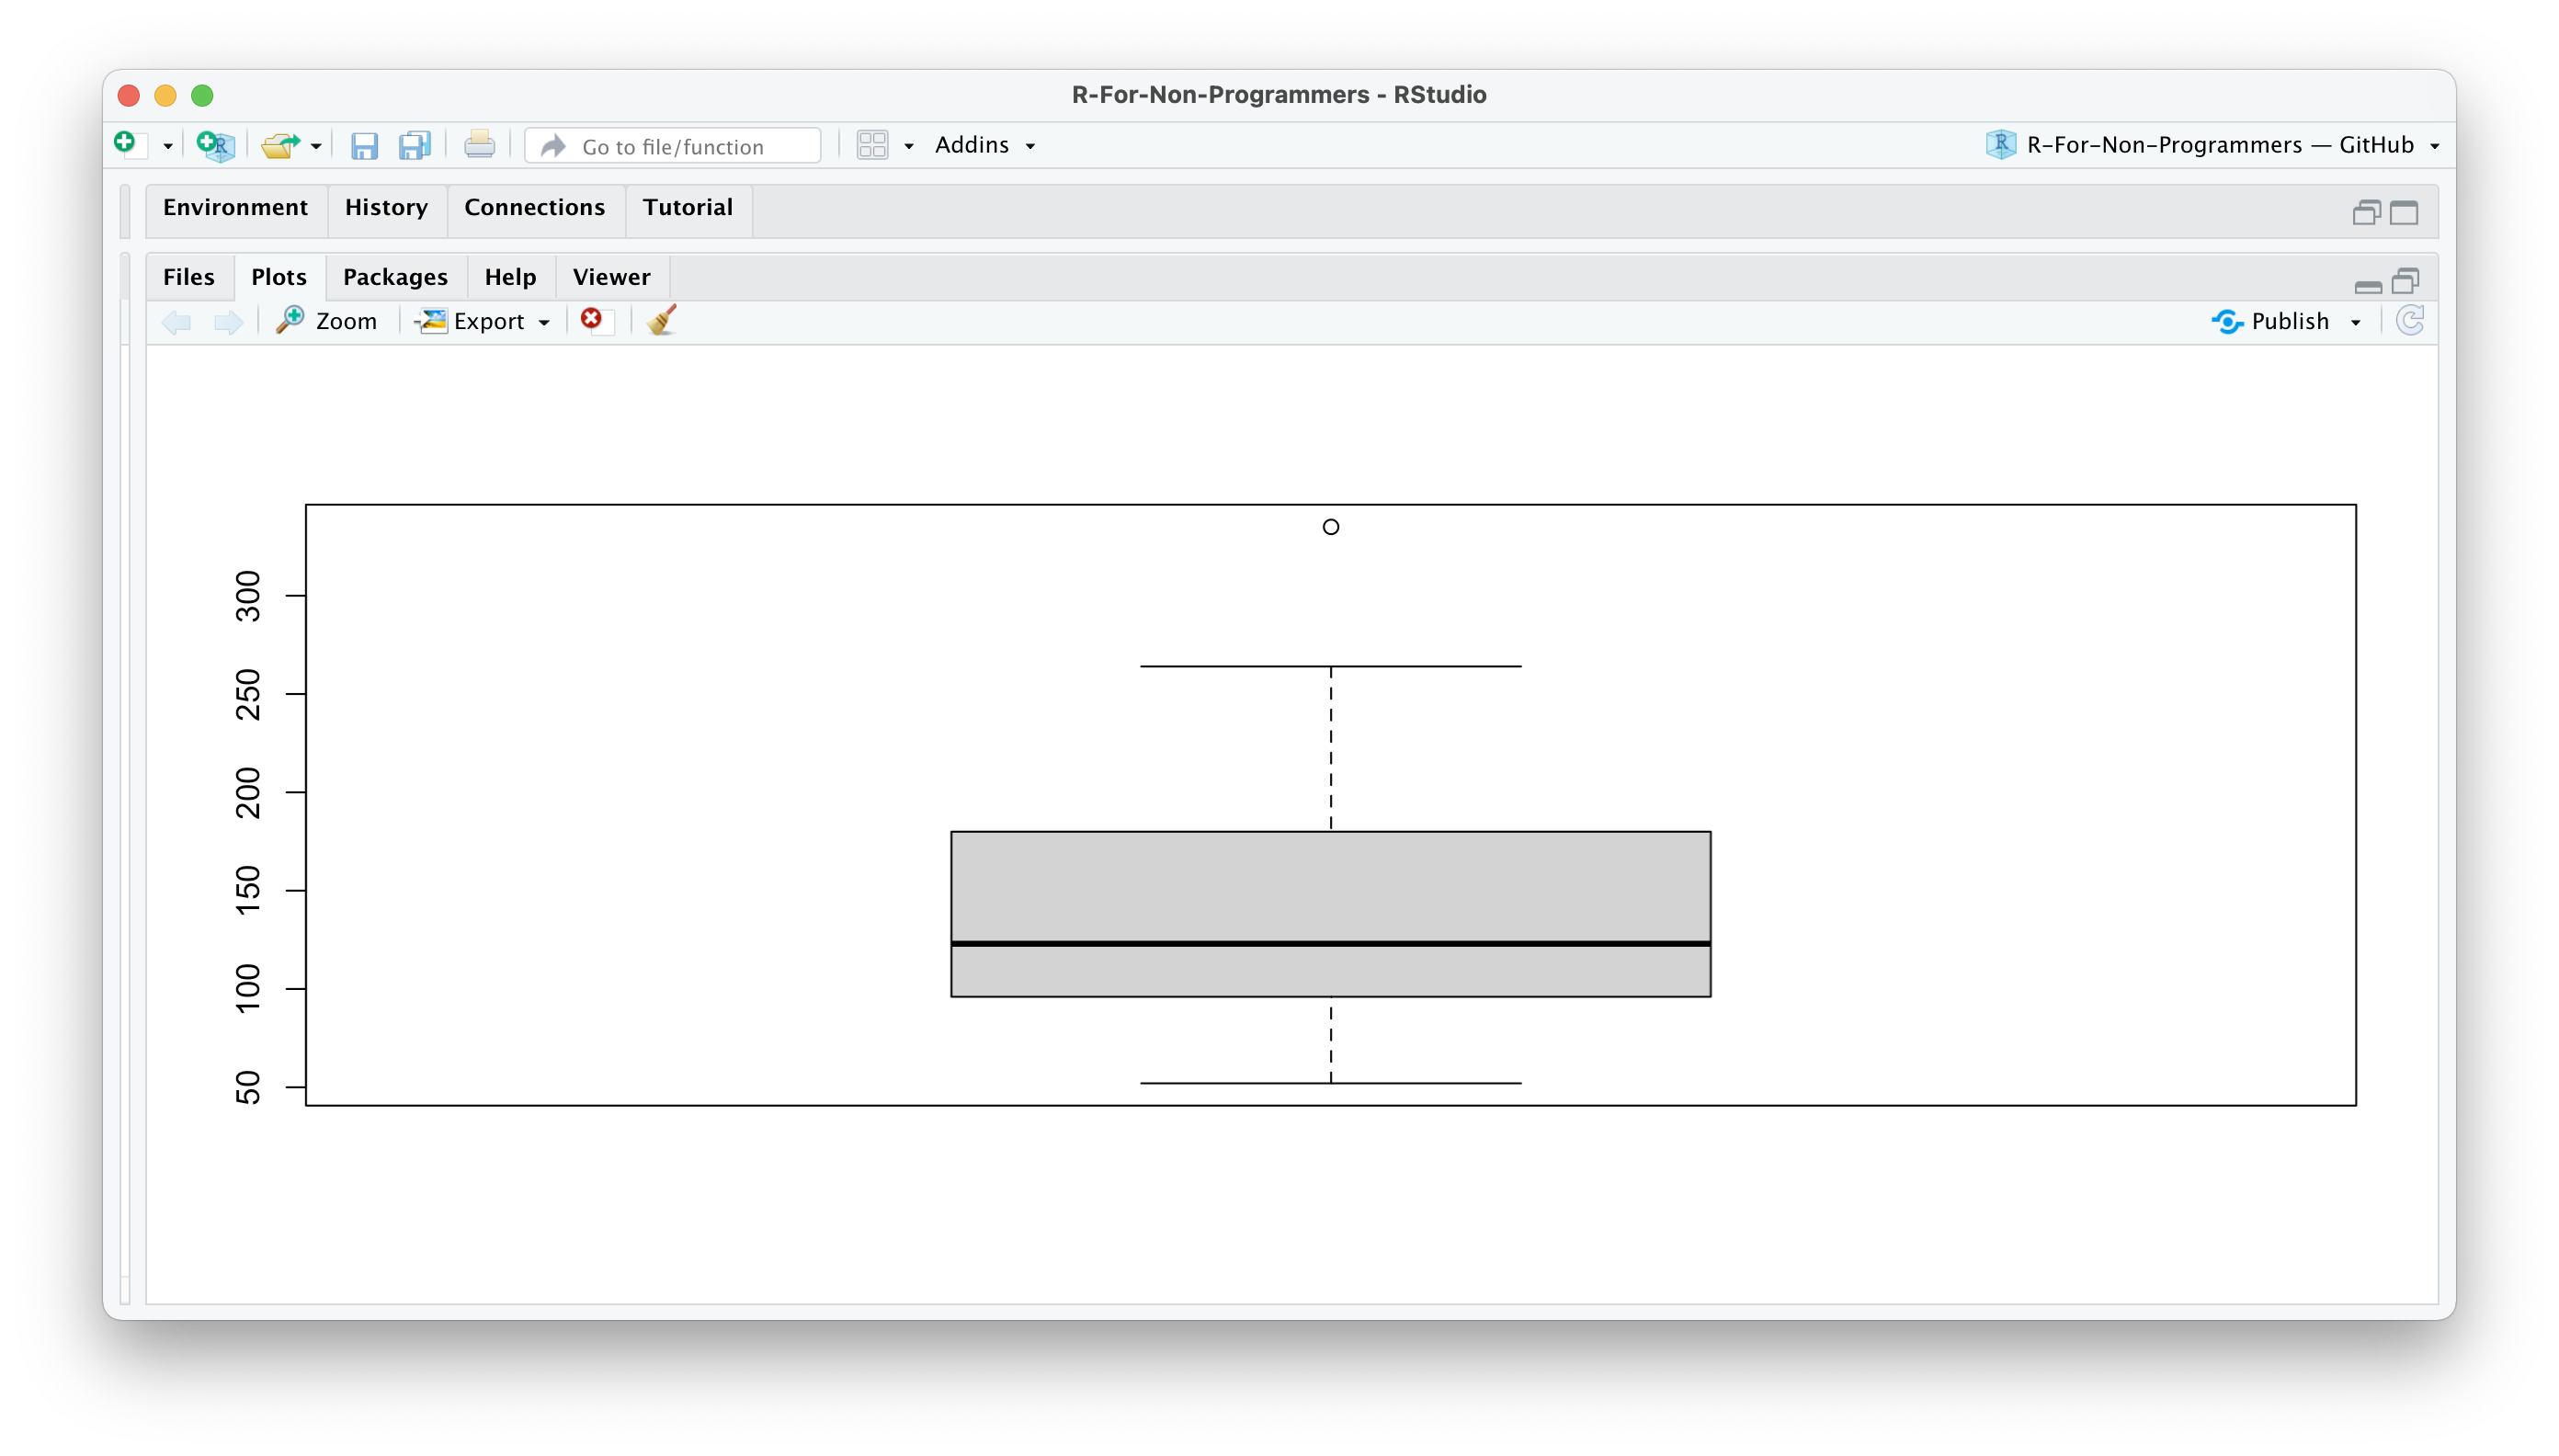
\includegraphics{images/chapter_04_img/05_files_plots_etc/02_rstudio_plots.png}

If you wish to delete the plot, you can click on the \texttt{red\ circle\ with\ a\ white\ x} symbol. This will delete the currently visible plot. If you wish to remove all plots from this pane, you can use the \texttt{broom}. There is also an option to export your plot and move back and forth between different plots.

Do not worry about the coding at this point. It will all make sense in the following chapters.

The next pane is called \emph{Packages}. Packages are additional tools you can import and use when performing your analysis. A frequent analogy people use to explain packages is your phone and the apps you install. Each package you download is equivalent to an app on your phone. It can enhance different aspects of working in \emph{R}, such as creating animated plots, using unique machine learning algorithms, or simply making your life easier by doing multiple computations with just one single line of code. You will learn more about \emph{R packages} in Chapter \ref{r-packages}.

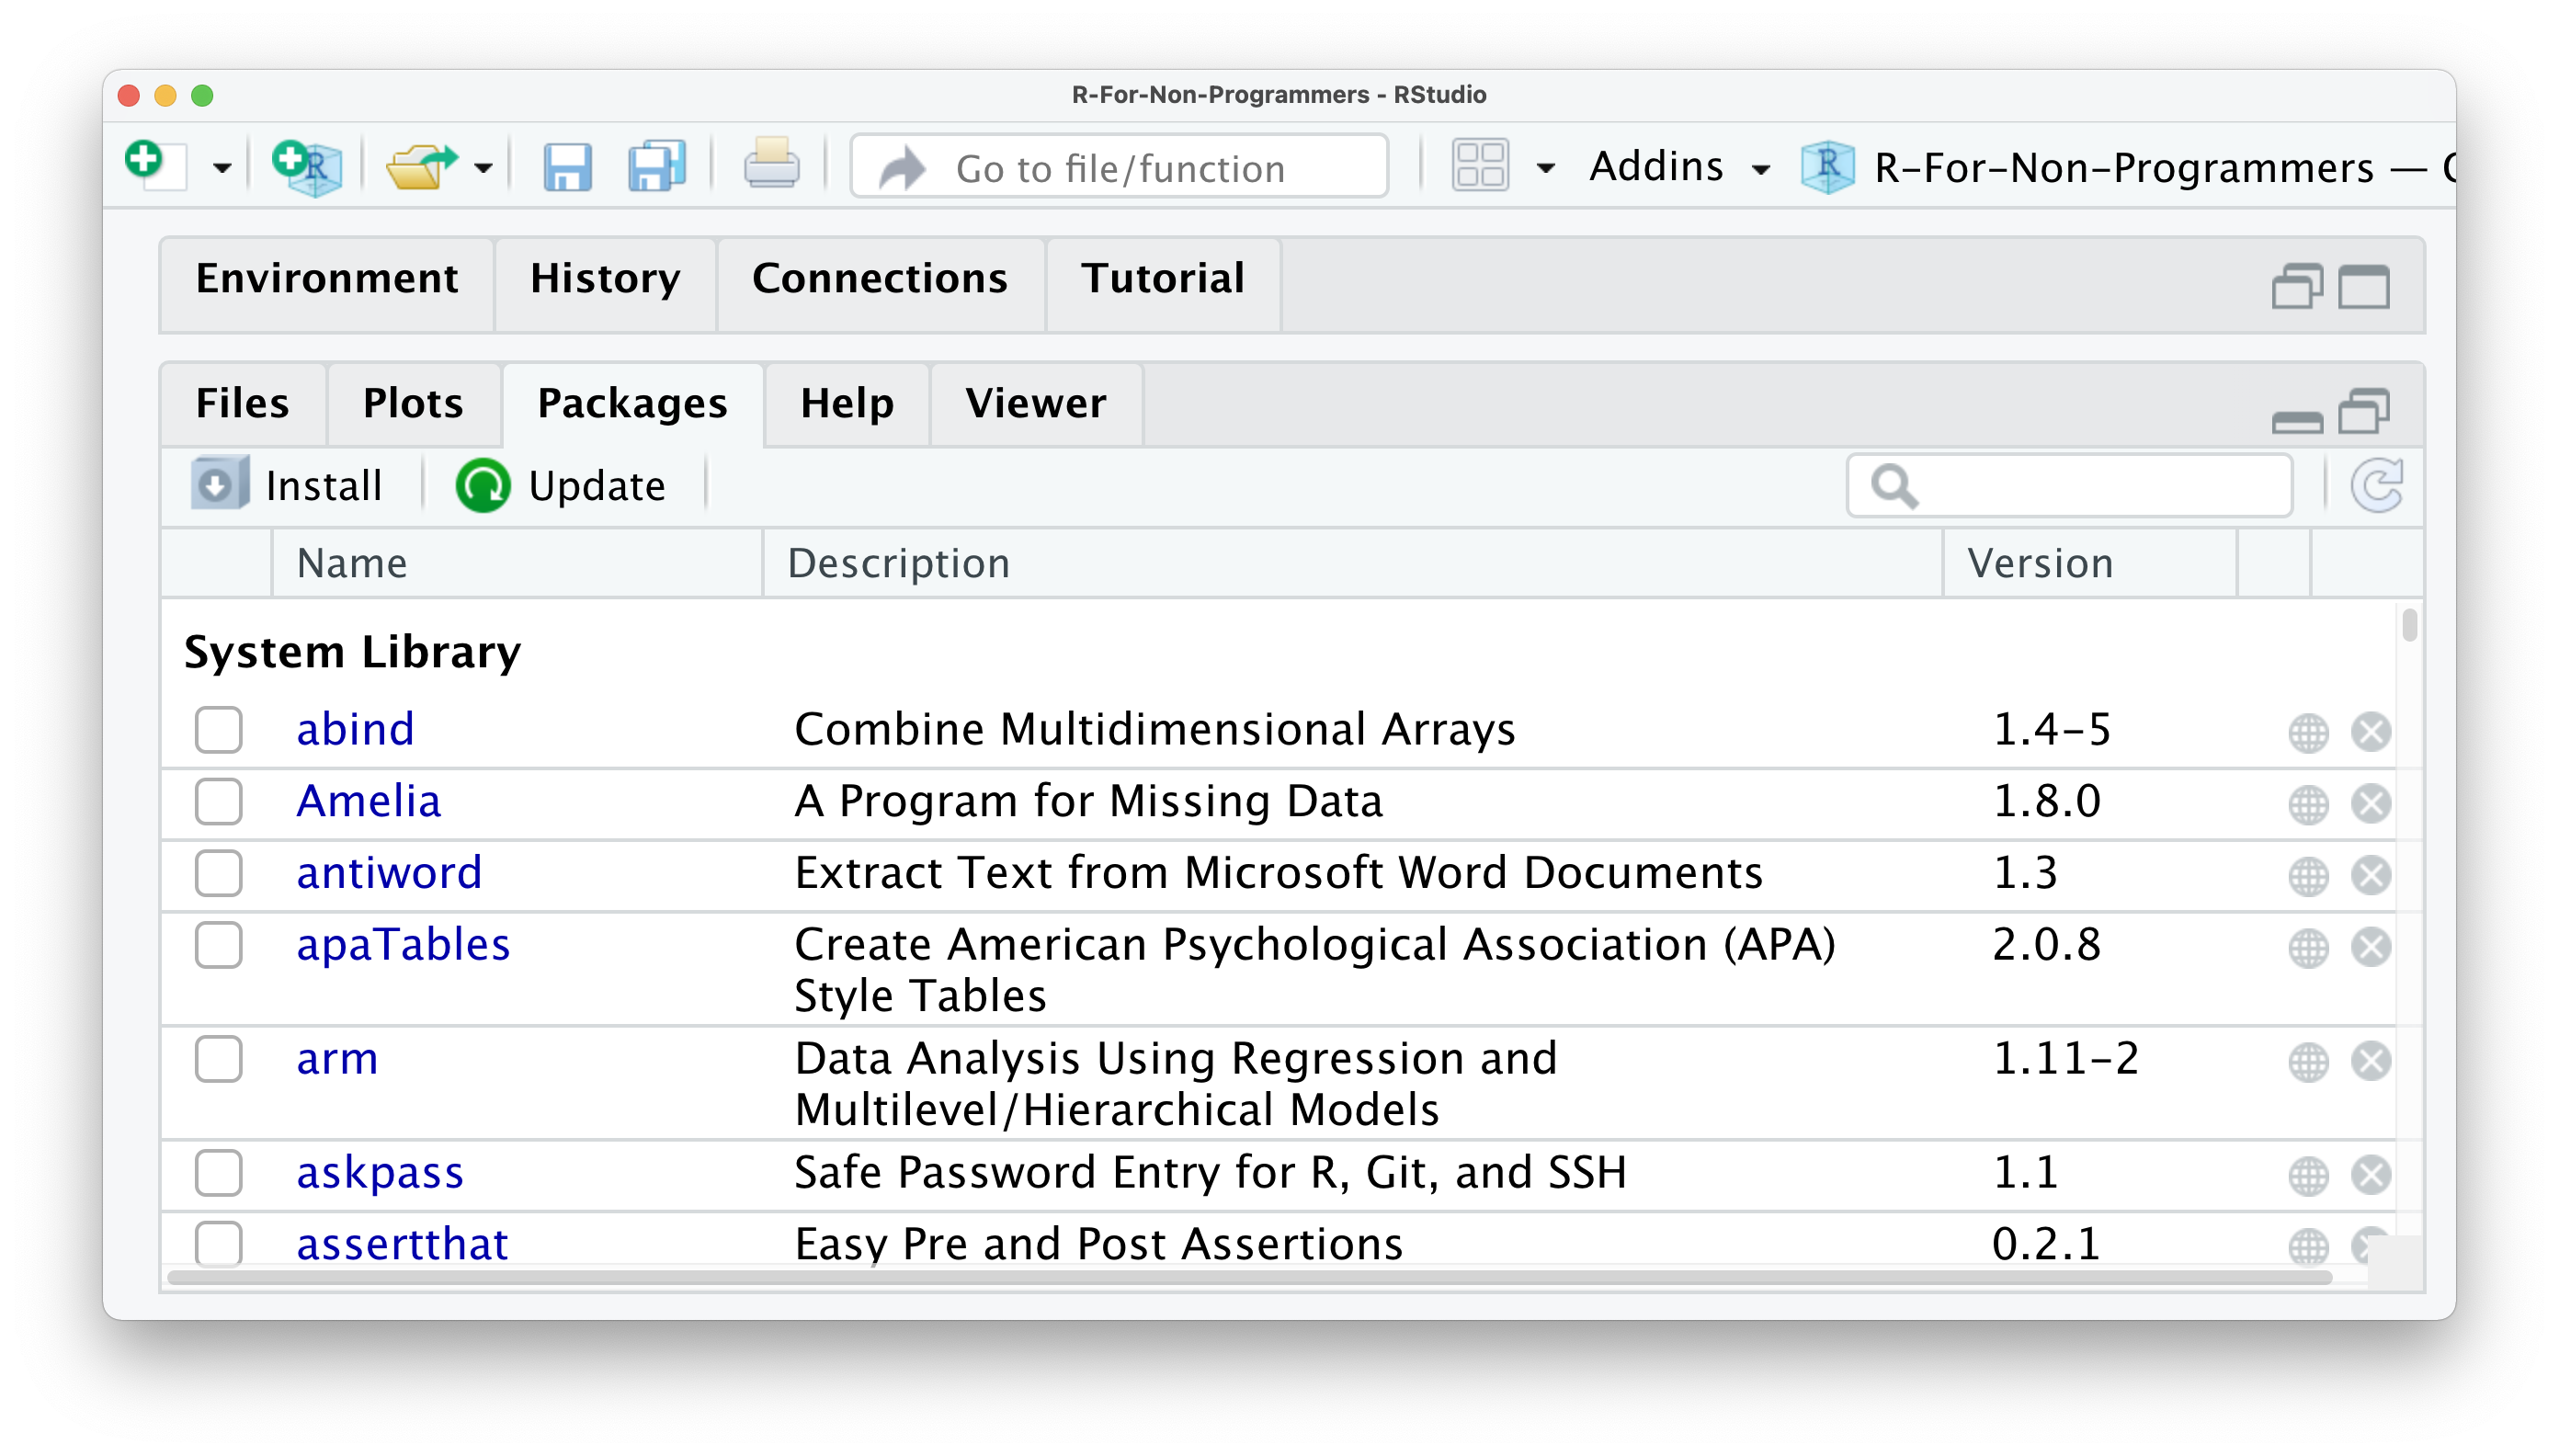
\includegraphics{images/chapter_04_img/05_files_plots_etc/03_rstudio_packages.png}

If you are in dire need of help, RStudio provides you with a \emph{Help} pane. You can search for specific topics, for example how certain computations work. The \emph{Help} pane also has documentation on different datasets that are included in \emph{R}, RStudio or \emph{R packages} you have installed. If you want a more comprehensive overview of how you can find help, have a look at CRAN's \href{https://www.r-project.org/help.html}{`Getting Help with R'} webpage.

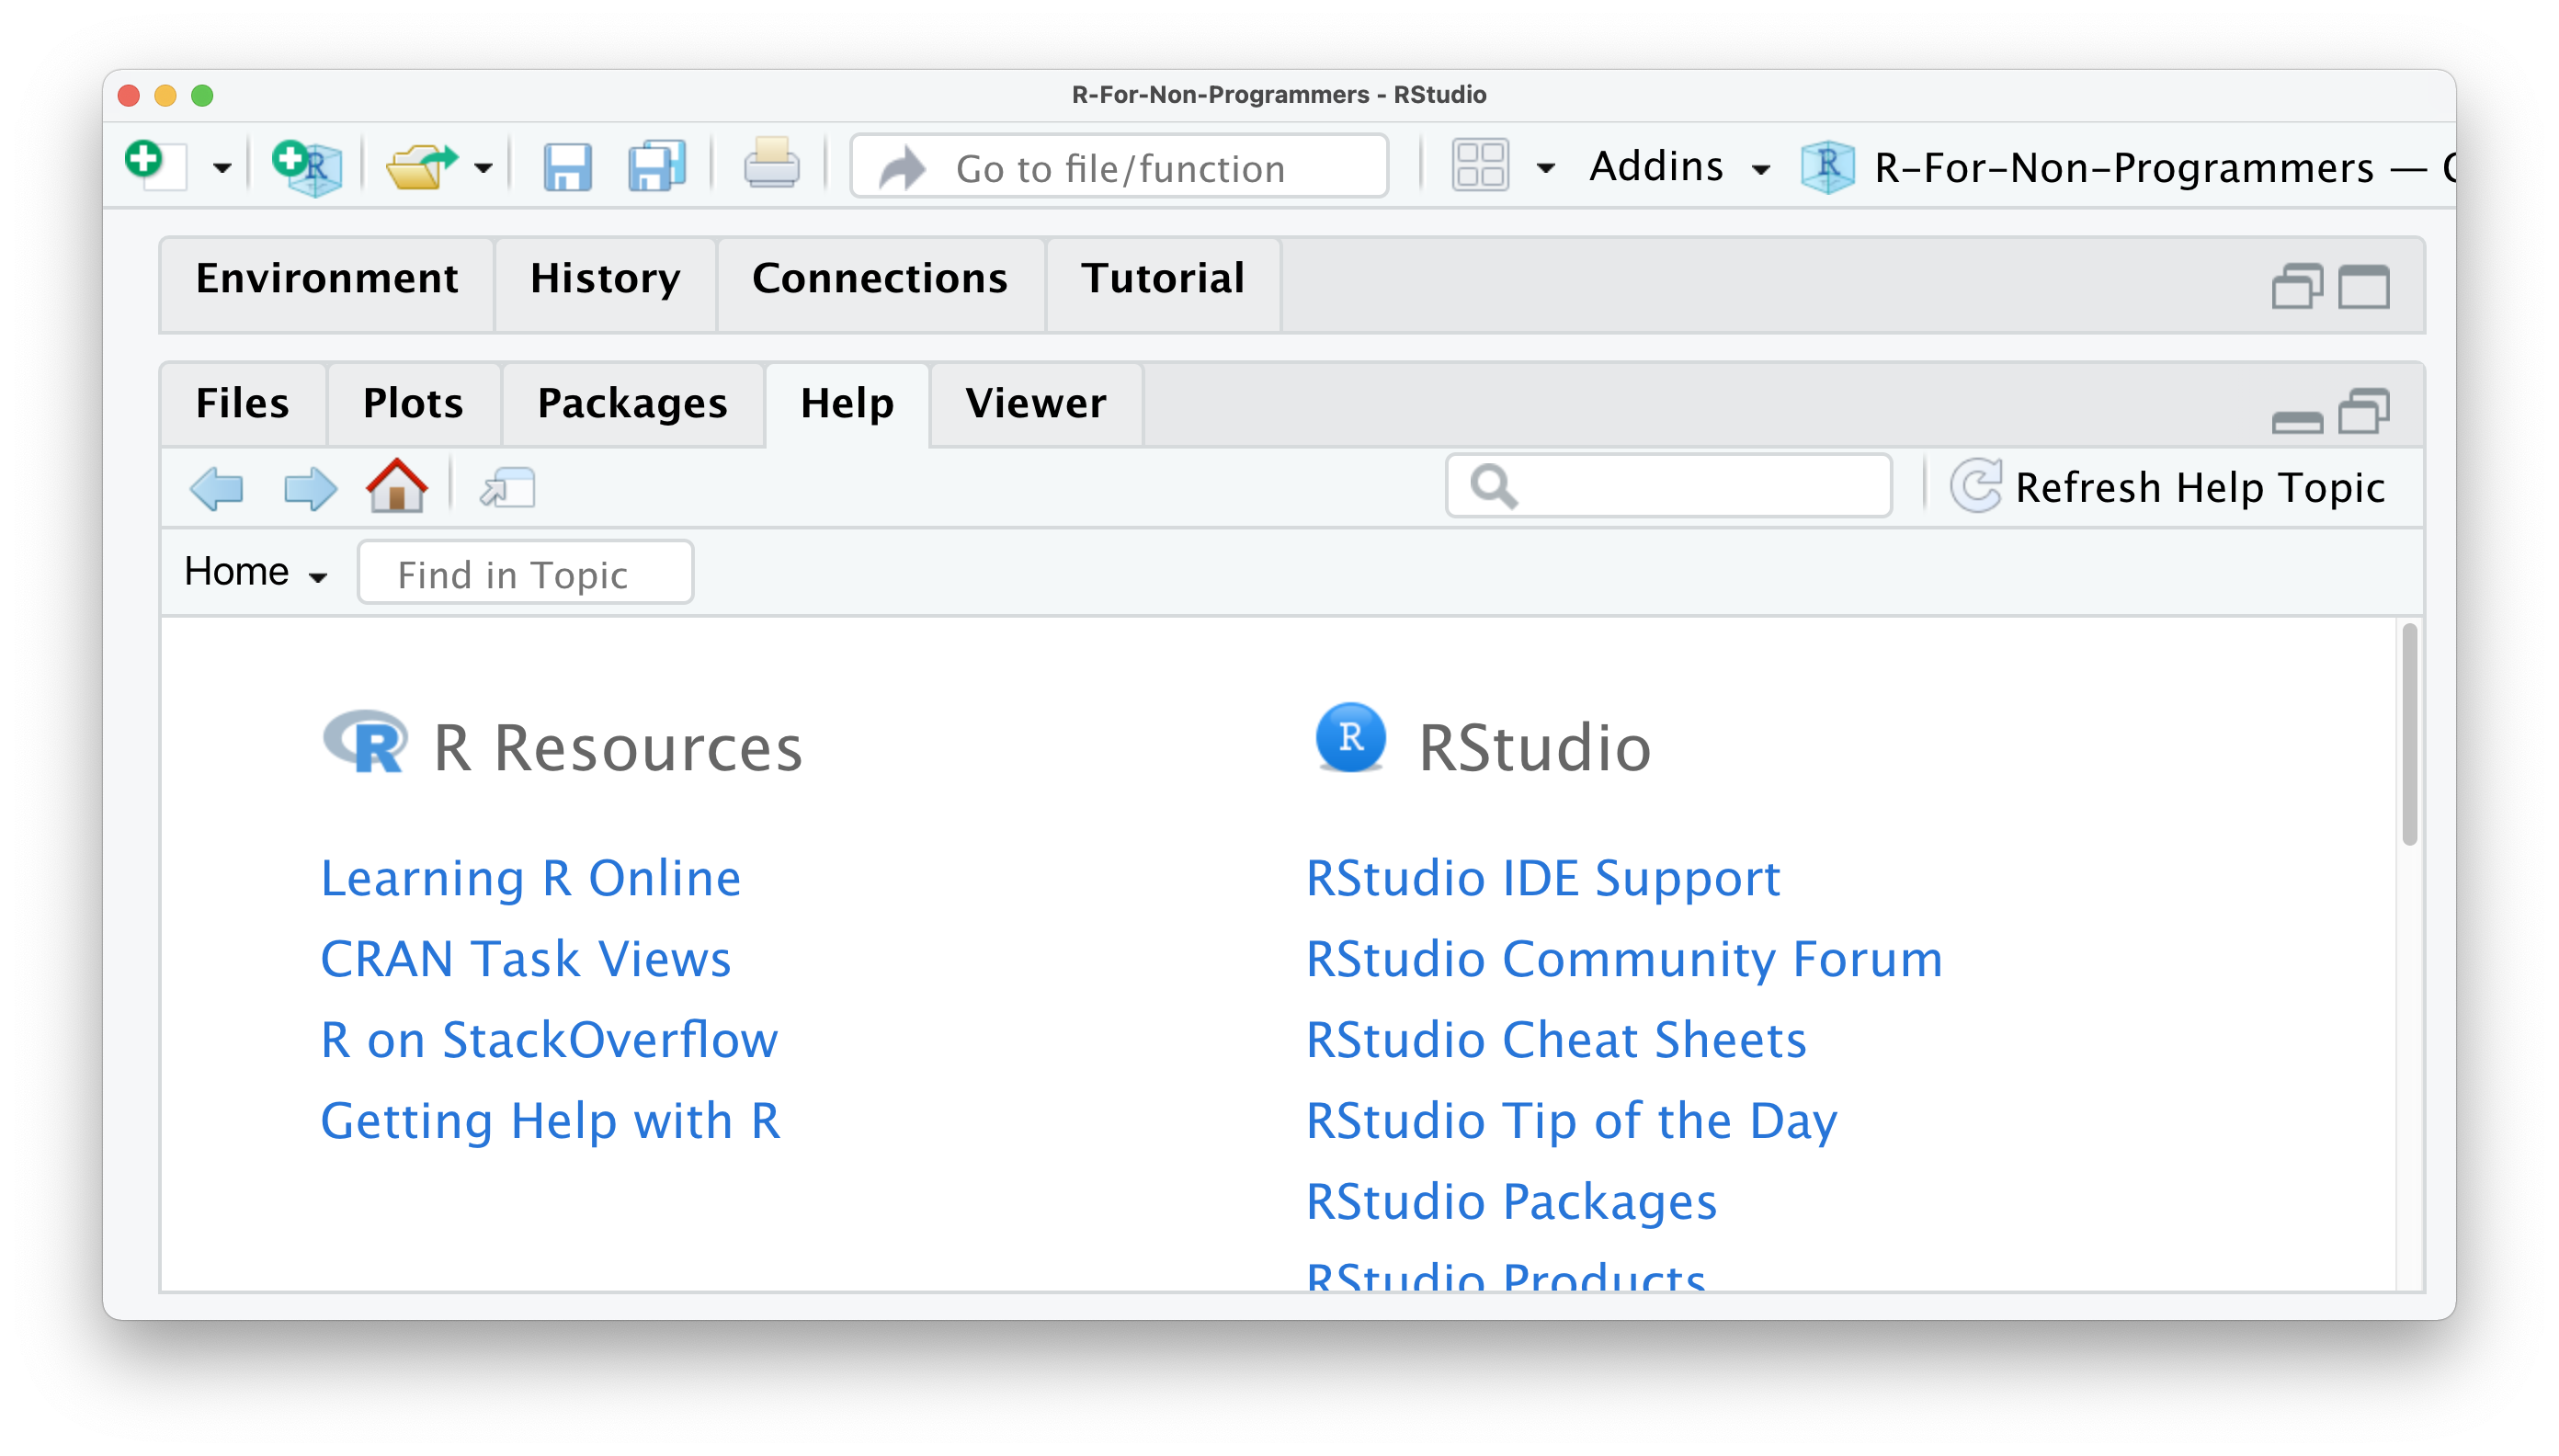
\includegraphics{images/chapter_04_img/05_files_plots_etc/04_rstudio_help.png}

So, for example, if you want to know what the \texttt{mtcars} dataset is, you can either use the search window in the \emph{Help} pane or, much easier, use a \texttt{?} in the console to search for it:

\begin{Shaded}
\begin{Highlighting}[]
\CommentTok{\# Type a \textquotesingle{}?\textquotesingle{} and immediately add the name to bring up helpful information.}

\NormalTok{?mtcars}
\end{Highlighting}
\end{Shaded}

This will open the \emph{Help} pane and give you more information about this dataset:

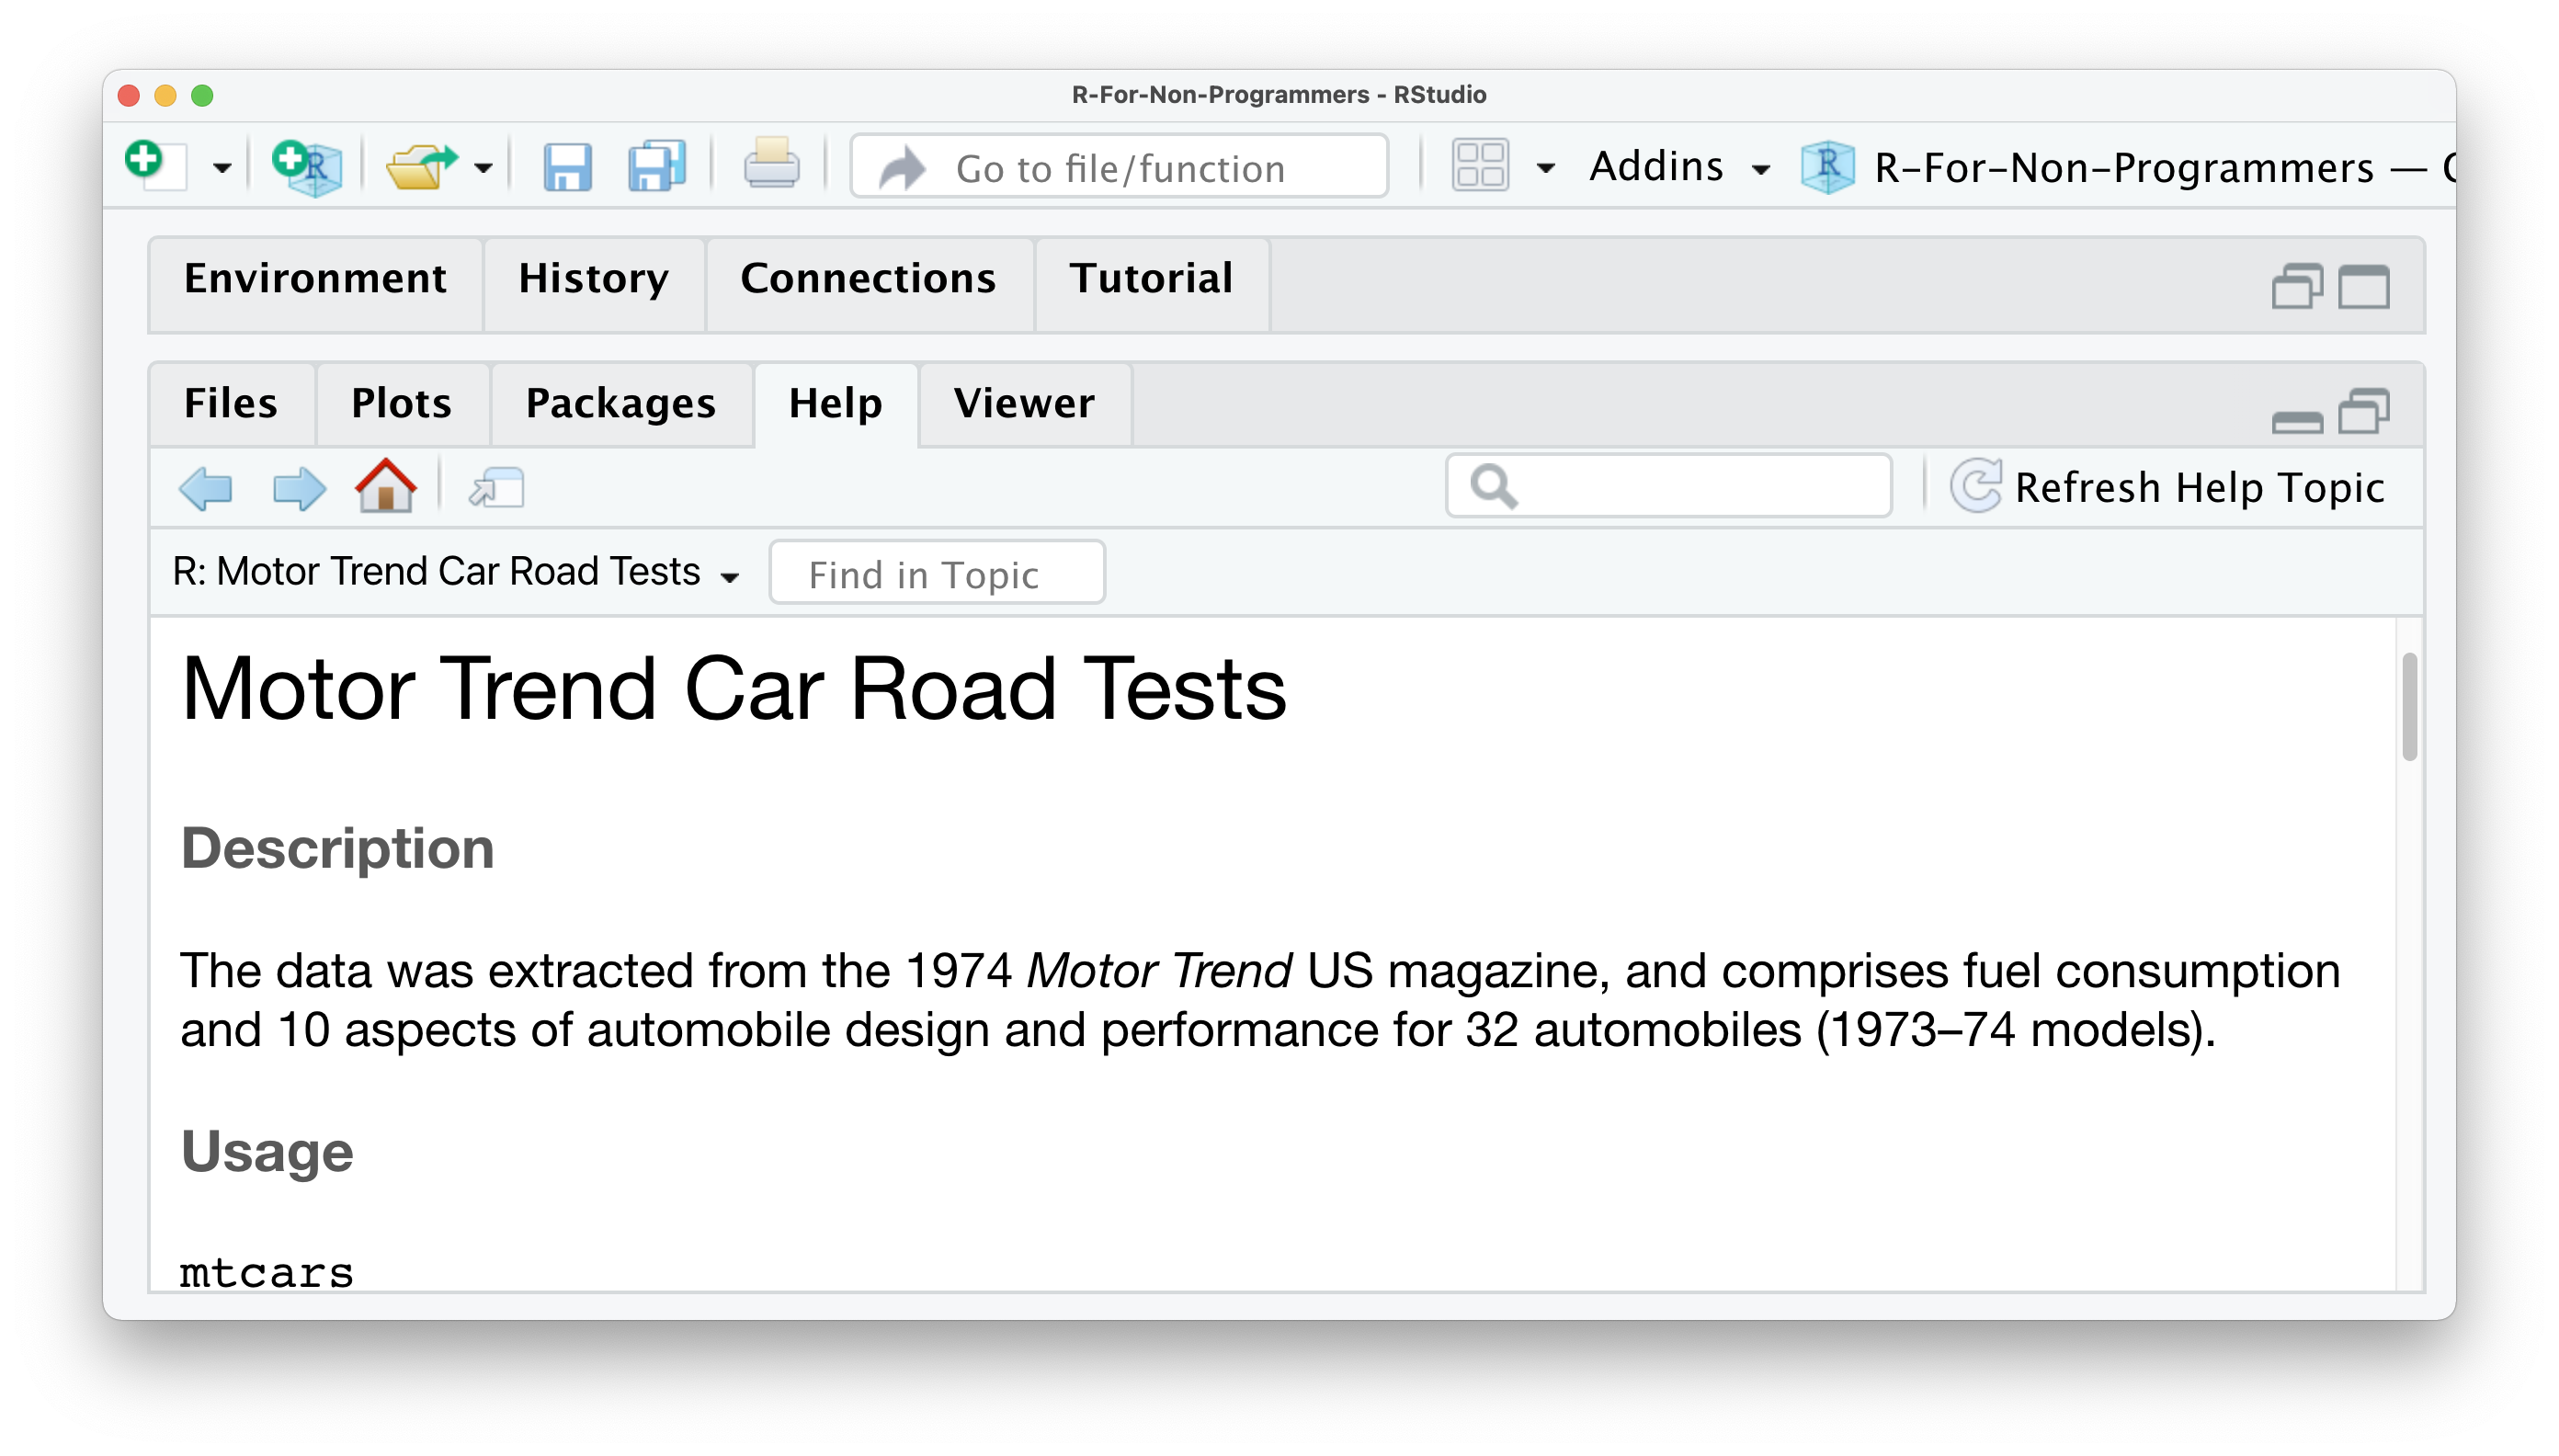
\includegraphics{images/chapter_04_img/05_files_plots_etc/04_rstudio_help_mtcars.png}

There are many different ways of how you can find help with your coding beyond RStudio and this book. My top three platforms to find solutions to my programming problems are:

\begin{itemize}
\item
  \href{https://www.google.com}{Google}
\item
  \href{https://stackoverflow.com}{stackoverflow.com}
\item
  \href{https://twitter.com/home}{Twitter} (with \href{https://twitter.com/hashtag/rstats}{\#RStats})
\end{itemize}

Lastly, we have the \emph{Viewer} pane. Not every data visualisation we create in R is a static image. You can create dynamic data visualisations or even websites with R. This type of content is displayed in the Viewer pane rather than in the Plots pane. Often these visualisations are based on HTML and other web-based programming languages. As such, it is easy to open them in your browser as well. However, in this book, we mainly focus on two-dimensional static plots, which are the ones you likely need most of the time, either for your assignments, thesis, or publication.

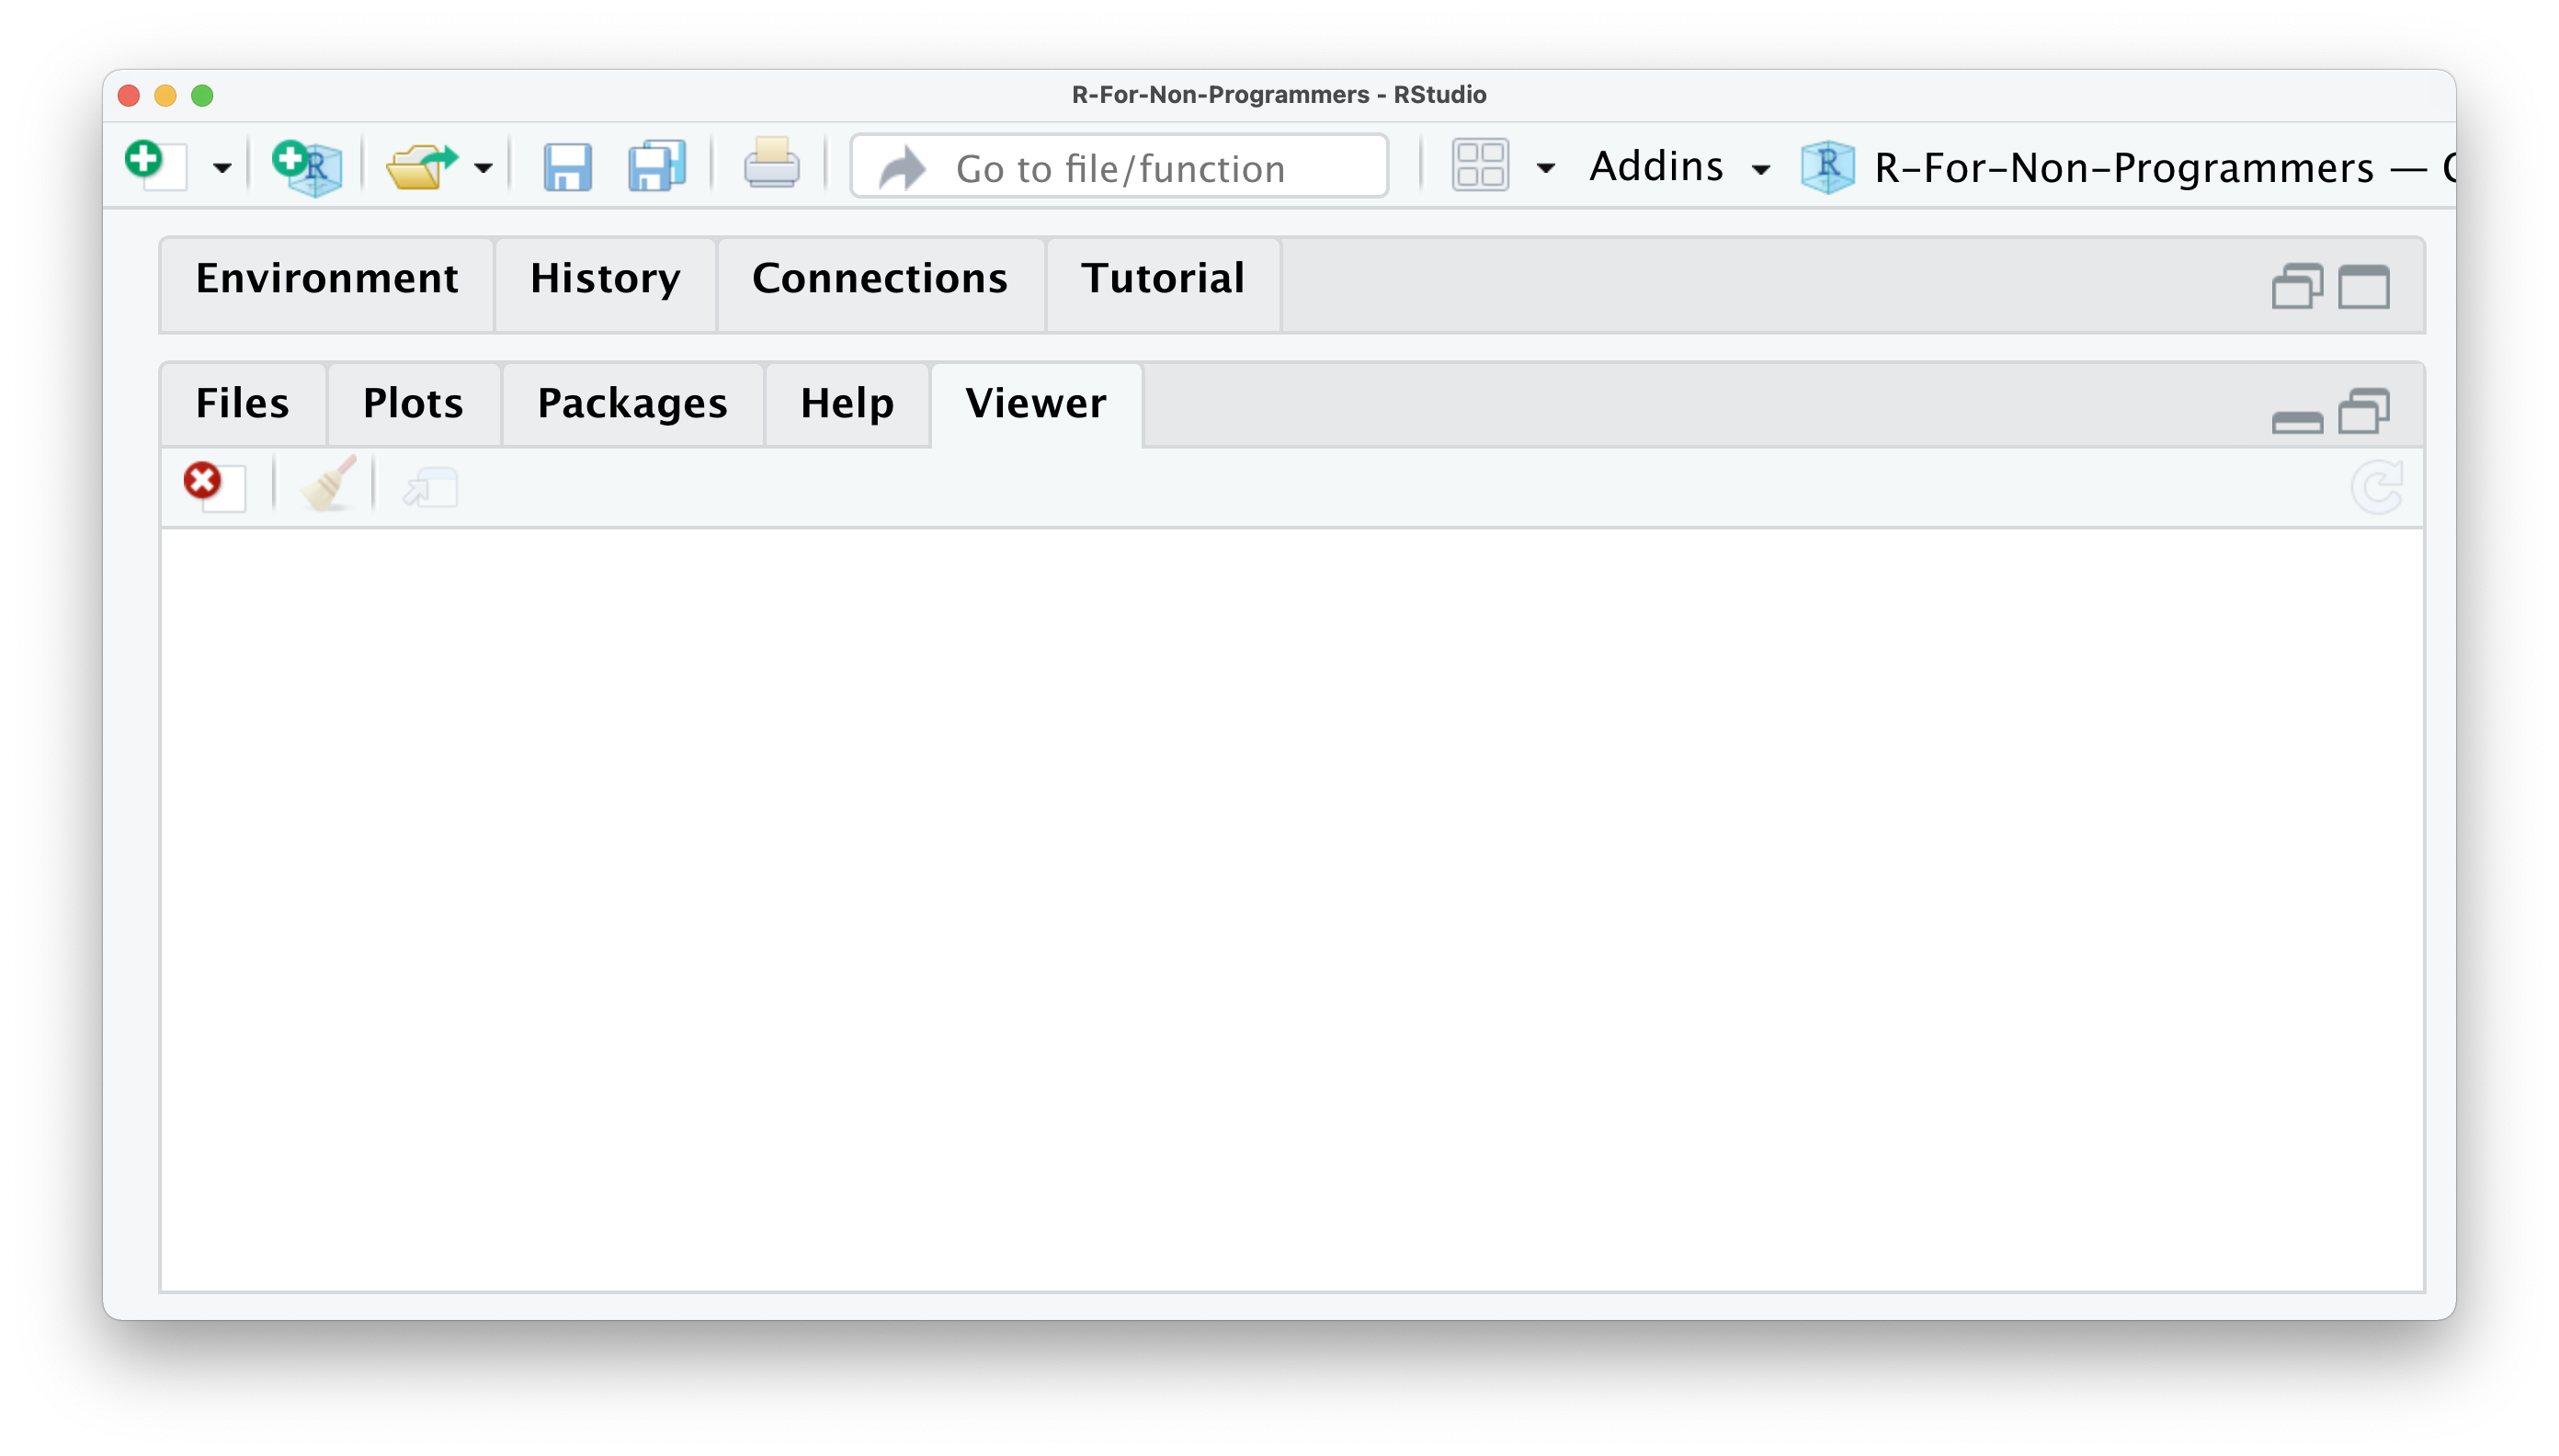
\includegraphics{images/chapter_04_img/05_files_plots_etc/05_rstudio_viewer.png}

\hypertarget{customise-your-user-interface}{%
\section{Customise your user interface}\label{customise-your-user-interface}}

As a last remark in this chapter, I would like to make you aware that you can modify each window. There are three basic adjustments you can make:

\begin{itemize}
\item
  Hide panes by clicking on the window symbol in the top right corner of each window,
\item
  Resize panes by dragging the border of a window horizontally or vertically, or
\item
  Add and remove panes by going to \texttt{RStudio\ \textgreater{}\ Preferences\ \textgreater{}\ Pane\ Layout}, or use the keyboard shortcut \texttt{⌘\ +\ ,} if you are on a Mac. There is, unfortunately no default shortcut for PC users.
\end{itemize}

If you want a fully customised experience you can also alter the colour scheme of the RStudio itself (\texttt{RStudio\ \textgreater{}\ Preferences\ \textgreater{}\ Appearance}) and if the themes offered are not enough for you, you can create a custom theme \href{https://tmtheme-editor.herokuapp.com/\#!/editor/theme/Monokai}{here}

\hypertarget{r-basics-the-very-fundamentals}{%
\chapter{R Basics: The very fundamentals}\label{r-basics-the-very-fundamentals}}

After a likely tedious installation of R and RStudio, as well as a somewhat detailed introduction to the RStudio interface, you are finally ready to `do' things. By `doing', I mean coding. The term `coding' in itself can instil fear in some of you, but you only need one skill to do it: Writing. As mentioned earlier, learning coding or programming means learning a new language. However, once you have the basic grammar down, you already can communicate quite a bit. In this section, we will explore the fundamentals of R. These build the foundation for everything that follows. After that, we dive right into some analysis.

\hypertarget{basic-computations-in-r}{%
\section{Basic computations in R}\label{basic-computations-in-r}}

The most basic computation you can do in R is arithmetic operations. In other words, addition, subtraction, multiplication, division, exponentiation and extraction of roots. In other words, R can be used like your pocket calculator, or more likely the one you have on your phone. For example, in Chapter \ref{the-console-window} we already performed an addition. Thus, it might not come as a surprise how their equivalents work in R. Let's take a look at the following examples:

\begin{Shaded}
\begin{Highlighting}[]
\CommentTok{\# Addition}
\DecValTok{10} \SpecialCharTok{+} \DecValTok{5}
\DocumentationTok{\#\# [1] 15}
\CommentTok{\# Subtraction}
\DecValTok{10} \SpecialCharTok{{-}} \DecValTok{5}
\DocumentationTok{\#\# [1] 5}
\CommentTok{\# Multiplication}
\DecValTok{10} \SpecialCharTok{*} \DecValTok{5}
\DocumentationTok{\#\# [1] 50}
\CommentTok{\# Division}
\DecValTok{10} \SpecialCharTok{/} \DecValTok{5}
\DocumentationTok{\#\# [1] 2}
\CommentTok{\# Exponentiation}
\DecValTok{10} \SpecialCharTok{\^{}} \DecValTok{2}
\DocumentationTok{\#\# [1] 100}
\CommentTok{\# Square root}
\FunctionTok{sqrt}\NormalTok{(}\DecValTok{10}\NormalTok{)}
\DocumentationTok{\#\# [1] 3.162278}
\end{Highlighting}
\end{Shaded}

They all look fairly straightforward except for the extraction of roots. As you probably know, extracting the root would typically mean we use the symbol \(\sqrt{}\) on your calculator. To compute the square root in R, we have to use a function instead to perform the computation. So we first put the name of the function \texttt{sqrt} and then the value \texttt{10} within parenthesis \texttt{()}. This results in the following code: \texttt{sqrt(10)}. If we were to write this down in our report, we would write \(\sqrt[2]{10}\).

Functions are an essential part of R and programming in general. You will learn more about them in this chapter.Besides arithmetic operations, there are also logical queries you can perform. Logical queries always return either the value TRUE or FALSE. Here are some examples which make this clearer:

\begin{Shaded}
\begin{Highlighting}[]
\CommentTok{\#1 Is it TRUE or FALSE?}
\DecValTok{1} \SpecialCharTok{==} \DecValTok{1}
\DocumentationTok{\#\# [1] TRUE}
\CommentTok{\#2 Is 45 bigger than 55?}
\DecValTok{45} \SpecialCharTok{\textgreater{}} \DecValTok{55}
\DocumentationTok{\#\# [1] FALSE}
\CommentTok{\#3 Is 1982 bigger or equal to 1982?}
\DecValTok{1982} \SpecialCharTok{\textgreater{}=} \DecValTok{1982}
\DocumentationTok{\#\# [1] TRUE}
\CommentTok{\#4 Are these two words NOT the same?}
\StringTok{"Friends"} \SpecialCharTok{!=} \StringTok{"friends"}
\DocumentationTok{\#\# [1] TRUE}
\CommentTok{\#5 Are these sentences the same?}
\StringTok{"I love statistics"} \SpecialCharTok{==} \StringTok{"I love statistícs"}
\DocumentationTok{\#\# [1] FALSE}
\end{Highlighting}
\end{Shaded}

Reflecting on these examples, you might notice three important things:

\begin{enumerate}
\def\labelenumi{\arabic{enumi}.}
\tightlist
\item
  I used \texttt{==} instead of \texttt{=},
\item
  I can compare non-numerical values, i.e.~text, which is also known as \texttt{character} values, with each other,
\item
  The devil is in the details (considering \#5).
\end{enumerate}

One of the most common mistakes of R novices is the confusion around the \texttt{==} and \texttt{=} notation. While \texttt{==} represents \texttt{equal\ to}, \texttt{=} is used to assign a value to an object (for more details on assignments see Chapter \ref{the-files-plots-packages-help-viewer-window}). However, in practice, most R programmers tend to avoid \texttt{=} since it can easily lead to confusion with \texttt{==}. As such, you can strike this one out of your R vocabulary for now.

There are many different logical operations you can perform. Table \ref{tab:logical-operators-r} lists the most frequently used logical operators for your reference. These will become important once we select only certain parts of our data for analysis, e.g.~only \texttt{female} participants.

\begin{longtable}[]{@{}ll@{}}
\caption{\label{tab:logical-operators-r} Logical Operators in R}\tabularnewline
\toprule
Operator & Description \\
\midrule
\endfirsthead
\toprule
Operator & Description \\
\midrule
\endhead
== & is equal to \\
\textgreater= & is bigger or equal to \\
\textless= & is smaller of equal to \\
!= & is not equal to \\
a \textbar{} b & a or b \\
a \& b & a and b \\
!a & is not a \\
\bottomrule
\end{longtable}

\hypertarget{assigning-values-to-objects}{%
\section{Assigning values to objects: `\textless-'}\label{assigning-values-to-objects}}

Another common task you will perform is assigning values to an object. An object can be many different things:

\begin{itemize}
\item
  a dataset,
\item
  the results of a computation,
\item
  a plot,
\item
  a series of numbers,
\item
  a list of names,
\item
  a function,
\item
  etc.
\end{itemize}

In short, an object is an umbrella term for many different things which form part of your data analysis. For example, objects are handy when storing results that you want to process further in later analytical steps. Let's have a look at an example.

\begin{Shaded}
\begin{Highlighting}[]
\CommentTok{\# I have a friend called "Fiona"}
\NormalTok{friends }\OtherTok{\textless{}{-}} \StringTok{"Fiona"}
\end{Highlighting}
\end{Shaded}

In this example, I created an object called \texttt{friends} and added \texttt{"Fiona"} to it. Remember, because \texttt{"Fiona"} represents a \texttt{string}, we need \texttt{""}. So, if you wanted to read this line of code, you would say, `\texttt{friends} gets the value \texttt{"Fiona"}'. Alternatively, you could also say `\texttt{"Fiona"} is assigned to \texttt{friends}'.

If you look into your environment pane, you will find the object we just created. You can see it carries the value \texttt{"Fiona"}. We can also print values of an object in the console by simply typing the name of the object \texttt{friends} and hit \texttt{Return\ ↵}.

\begin{Shaded}
\begin{Highlighting}[]
\CommentTok{\# Who are my friends?}
\NormalTok{friends}
\DocumentationTok{\#\# [1] "Fiona"}
\end{Highlighting}
\end{Shaded}

Sadly, it seems I only have one friend. Luckily we can add some more, not the least to make me feel less lonely. To create objects with multiple values, we can use the function \texttt{c()}, which stands for `concatenate'. The \citet{concatenate-2021} define this word as follows:

\begin{quote}
`\textbf{\emph{concatenate}}',

to put things together as a connected series
\end{quote}

Let's concatenate some more friends into our \texttt{friends} object.

\begin{Shaded}
\begin{Highlighting}[]
\CommentTok{\# Adding some more friends to my life}
\NormalTok{friends }\OtherTok{\textless{}{-}} \FunctionTok{c}\NormalTok{(}\StringTok{"Fiona"}\NormalTok{, }\StringTok{"Ida"}\NormalTok{, }\StringTok{"Lukas"}\NormalTok{, }\StringTok{"Georg"}\NormalTok{, }\StringTok{"Daniel"}\NormalTok{, }\StringTok{"Pavel"}\NormalTok{, }\StringTok{"Tigger"}\NormalTok{)}

\CommentTok{\# Here are all my friends}
\NormalTok{friends}
\DocumentationTok{\#\# [1] "Fiona"  "Ida"    "Lukas"  "Georg"  "Daniel" "Pavel"  "Tigger"}
\end{Highlighting}
\end{Shaded}

To concatenate values into a single object, we need to use a comma \texttt{,} to separate each value. Otherwise, R will report an error back.

\begin{Shaded}
\begin{Highlighting}[]
\NormalTok{friends }\OtherTok{\textless{}{-}} \FunctionTok{c}\NormalTok{(}\StringTok{"Fiona"} \StringTok{"Ida"}\NormalTok{)}
\DocumentationTok{\#\# Error: \textless{}text\textgreater{}:1:22: unexpected string constant}
\DocumentationTok{\#\# 1: friends \textless{}{-} c("Fiona" "Ida"}
\DocumentationTok{\#\#                          \^{}}
\end{Highlighting}
\end{Shaded}

R's error messages tend to be very useful and give meaningful clues to what went wrong. In this case, we can see that something `unexpected' happen, and it shows where our mistake is.

You can also concatenate numbers, and if you add \texttt{()} around it, you can automatically print the content of the object to the console. Thus, \texttt{(milestones\_of\_my\_life\ \textless{}-\ c(1982,\ 2006,\ 2011,\ 2018,\ 2020))} is the same as \texttt{milestones\_of\_my\_life\ \textless{}-\ c(1982,\ 2006,\ 2011,\ 2018,\ 2020)} followed by \texttt{milestones\_of\_my\_life}. The following examples illustrate this.

\begin{Shaded}
\begin{Highlighting}[]
\CommentTok{\# Important years in my life}
\NormalTok{milestones\_of\_my\_life }\OtherTok{\textless{}{-}} \FunctionTok{c}\NormalTok{(}\DecValTok{1982}\NormalTok{, }\DecValTok{2006}\NormalTok{, }\DecValTok{2011}\NormalTok{, }\DecValTok{2018}\NormalTok{, }\DecValTok{2020}\NormalTok{)}
\NormalTok{milestones\_of\_my\_life}
\DocumentationTok{\#\# [1] 1982 2006 2011 2018 2020}
\CommentTok{\# The same as above, but we don\textquotesingle{}t need the second line of code}
\NormalTok{(milestones\_of\_my\_life }\OtherTok{\textless{}{-}} \FunctionTok{c}\NormalTok{(}\DecValTok{1982}\NormalTok{, }\DecValTok{2006}\NormalTok{, }\DecValTok{2011}\NormalTok{, }\DecValTok{2018}\NormalTok{, }\DecValTok{2020}\NormalTok{))}
\DocumentationTok{\#\# [1] 1982 2006 2011 2018 2020}
\end{Highlighting}
\end{Shaded}

Finally, we can also concatenate numbers and character values into one object:

\begin{Shaded}
\begin{Highlighting}[]
\NormalTok{(names\_and\_years }\OtherTok{\textless{}{-}} \FunctionTok{c}\NormalTok{(}\StringTok{"Fiona"}\NormalTok{, }\DecValTok{1988}\NormalTok{, }\StringTok{"Daniel"}\NormalTok{, }\DecValTok{1982}\NormalTok{))}
\DocumentationTok{\#\# [1] "Fiona"  "1988"   "Daniel" "1982"}
\end{Highlighting}
\end{Shaded}

This last example is not necessarily something I would recommend to do, because it likely leads to undesirable outcomes. If you look into your environment pane you currently have three objects: \texttt{friends}, \texttt{milestones\_of\_my\_life}, and \texttt{names\_and\_years}.

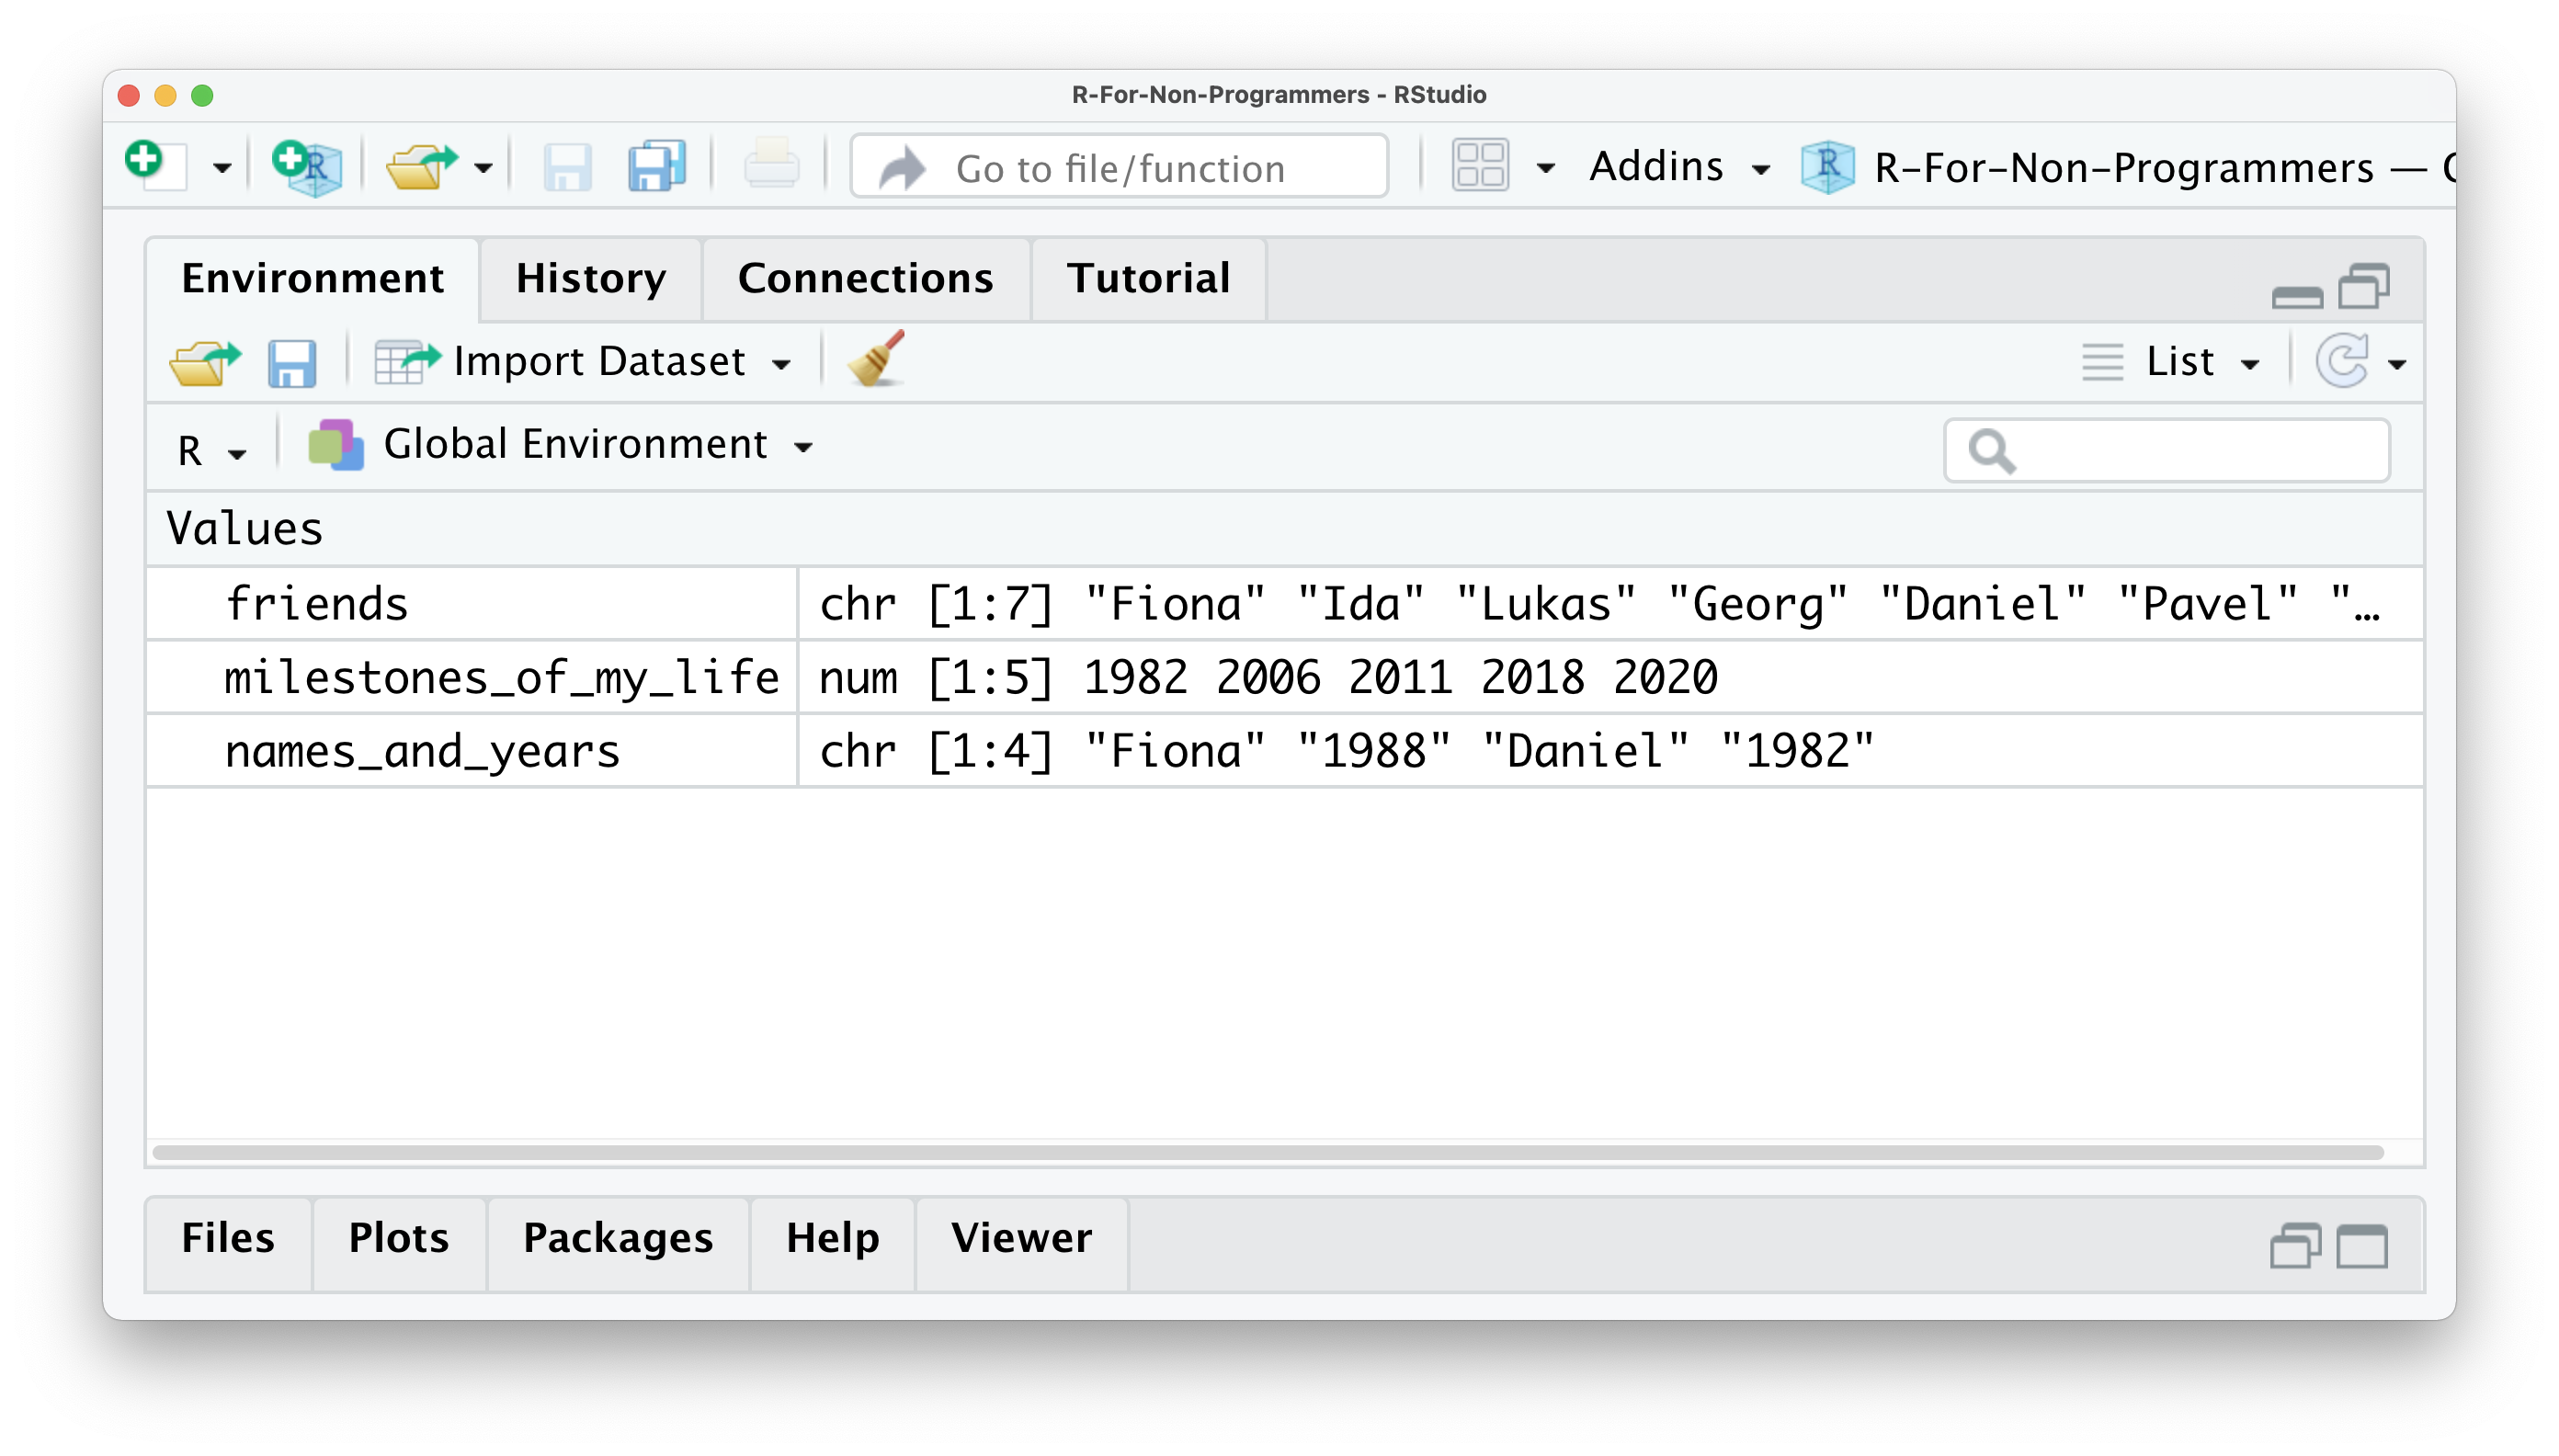
\includegraphics{images/chapter_05_img/01_basic_computation_environment_objects.png}

The \texttt{friends} object shows that all the values inside the object are classified as \texttt{chr}, which denominates \texttt{character}. In this case, this is correct because it only includes the names of my friends. On the other hand, the object \texttt{milestones\_of\_my\_life} only includes \texttt{numeric} values, and therefore it says \texttt{num} in the environment pane. However, for the object \texttt{names\_and\_years} we know we want to have \texttt{numeric} and \texttt{character} values included. Still, R recognises them as \texttt{character} values only because values inside objects are meant to be of the same type.

Consequently, mixing different types of data (as explained in Chapter @ref()) into one object is likely a bad idea. This is especially true if you want to use the numeric values for computation. In short: ensure your objects are all of the same data type.

There is an exception to this rule. `Of course', you might say. There is one object that can have values of different types: \texttt{list}. As the name indicates, a \texttt{list} object holds several items. These items are usually other objects. In the spirit of `\href{https://www.imdb.com/title/tt1375666/?ref_=ext_shr_lnk}{Inception}', you can have lists inside lists, which contain more objects.

Let's create a list called \texttt{x\_files} using the \texttt{list} function and place all our objects inside.

\begin{Shaded}
\begin{Highlighting}[]
\CommentTok{\# This creates our list of objects}
\NormalTok{x\_files }\OtherTok{\textless{}{-}} \FunctionTok{list}\NormalTok{(friends,}
\NormalTok{               milestones\_of\_my\_life,}
\NormalTok{               names\_and\_years)}

\CommentTok{\# Let\textquotesingle{}s have a look what is hidden inside the x\_files}
\NormalTok{x\_files}
\DocumentationTok{\#\# [[1]]}
\DocumentationTok{\#\# [1] "Fiona"  "Ida"    "Lukas"  "Georg"  "Daniel" "Pavel"  "Tigger"}
\DocumentationTok{\#\# }
\DocumentationTok{\#\# [[2]]}
\DocumentationTok{\#\# [1] 1982 2006 2011 2018 2020}
\DocumentationTok{\#\# }
\DocumentationTok{\#\# [[3]]}
\DocumentationTok{\#\# [1] "Fiona"  "1988"   "Daniel" "1982"}
\end{Highlighting}
\end{Shaded}

You will notice in this example that I do not use \texttt{""} for each value in the list. This is because \texttt{friends} is not a character I put into the list, but an object. When we refer to objects, we do not need quotation marks.

We will encounter \texttt{list} objects quite frequently when we perform our analysis. Some functions return the results in the format of lists. This can be very helpful because otherwise our environment pane will be littered with objects. We would not necessarily know how they relate to each other, or worse, to which analysis they belong. Looking at the list item in the environment page (Figure \ref{fig:img-x-files}), you can see that the object \texttt{x\_files} is classified as a \texttt{List\ of\ 3,} and if you click on the blue icon, you can inspect the different objects inside.

\textbackslash begin\{figure\}

\{\centering 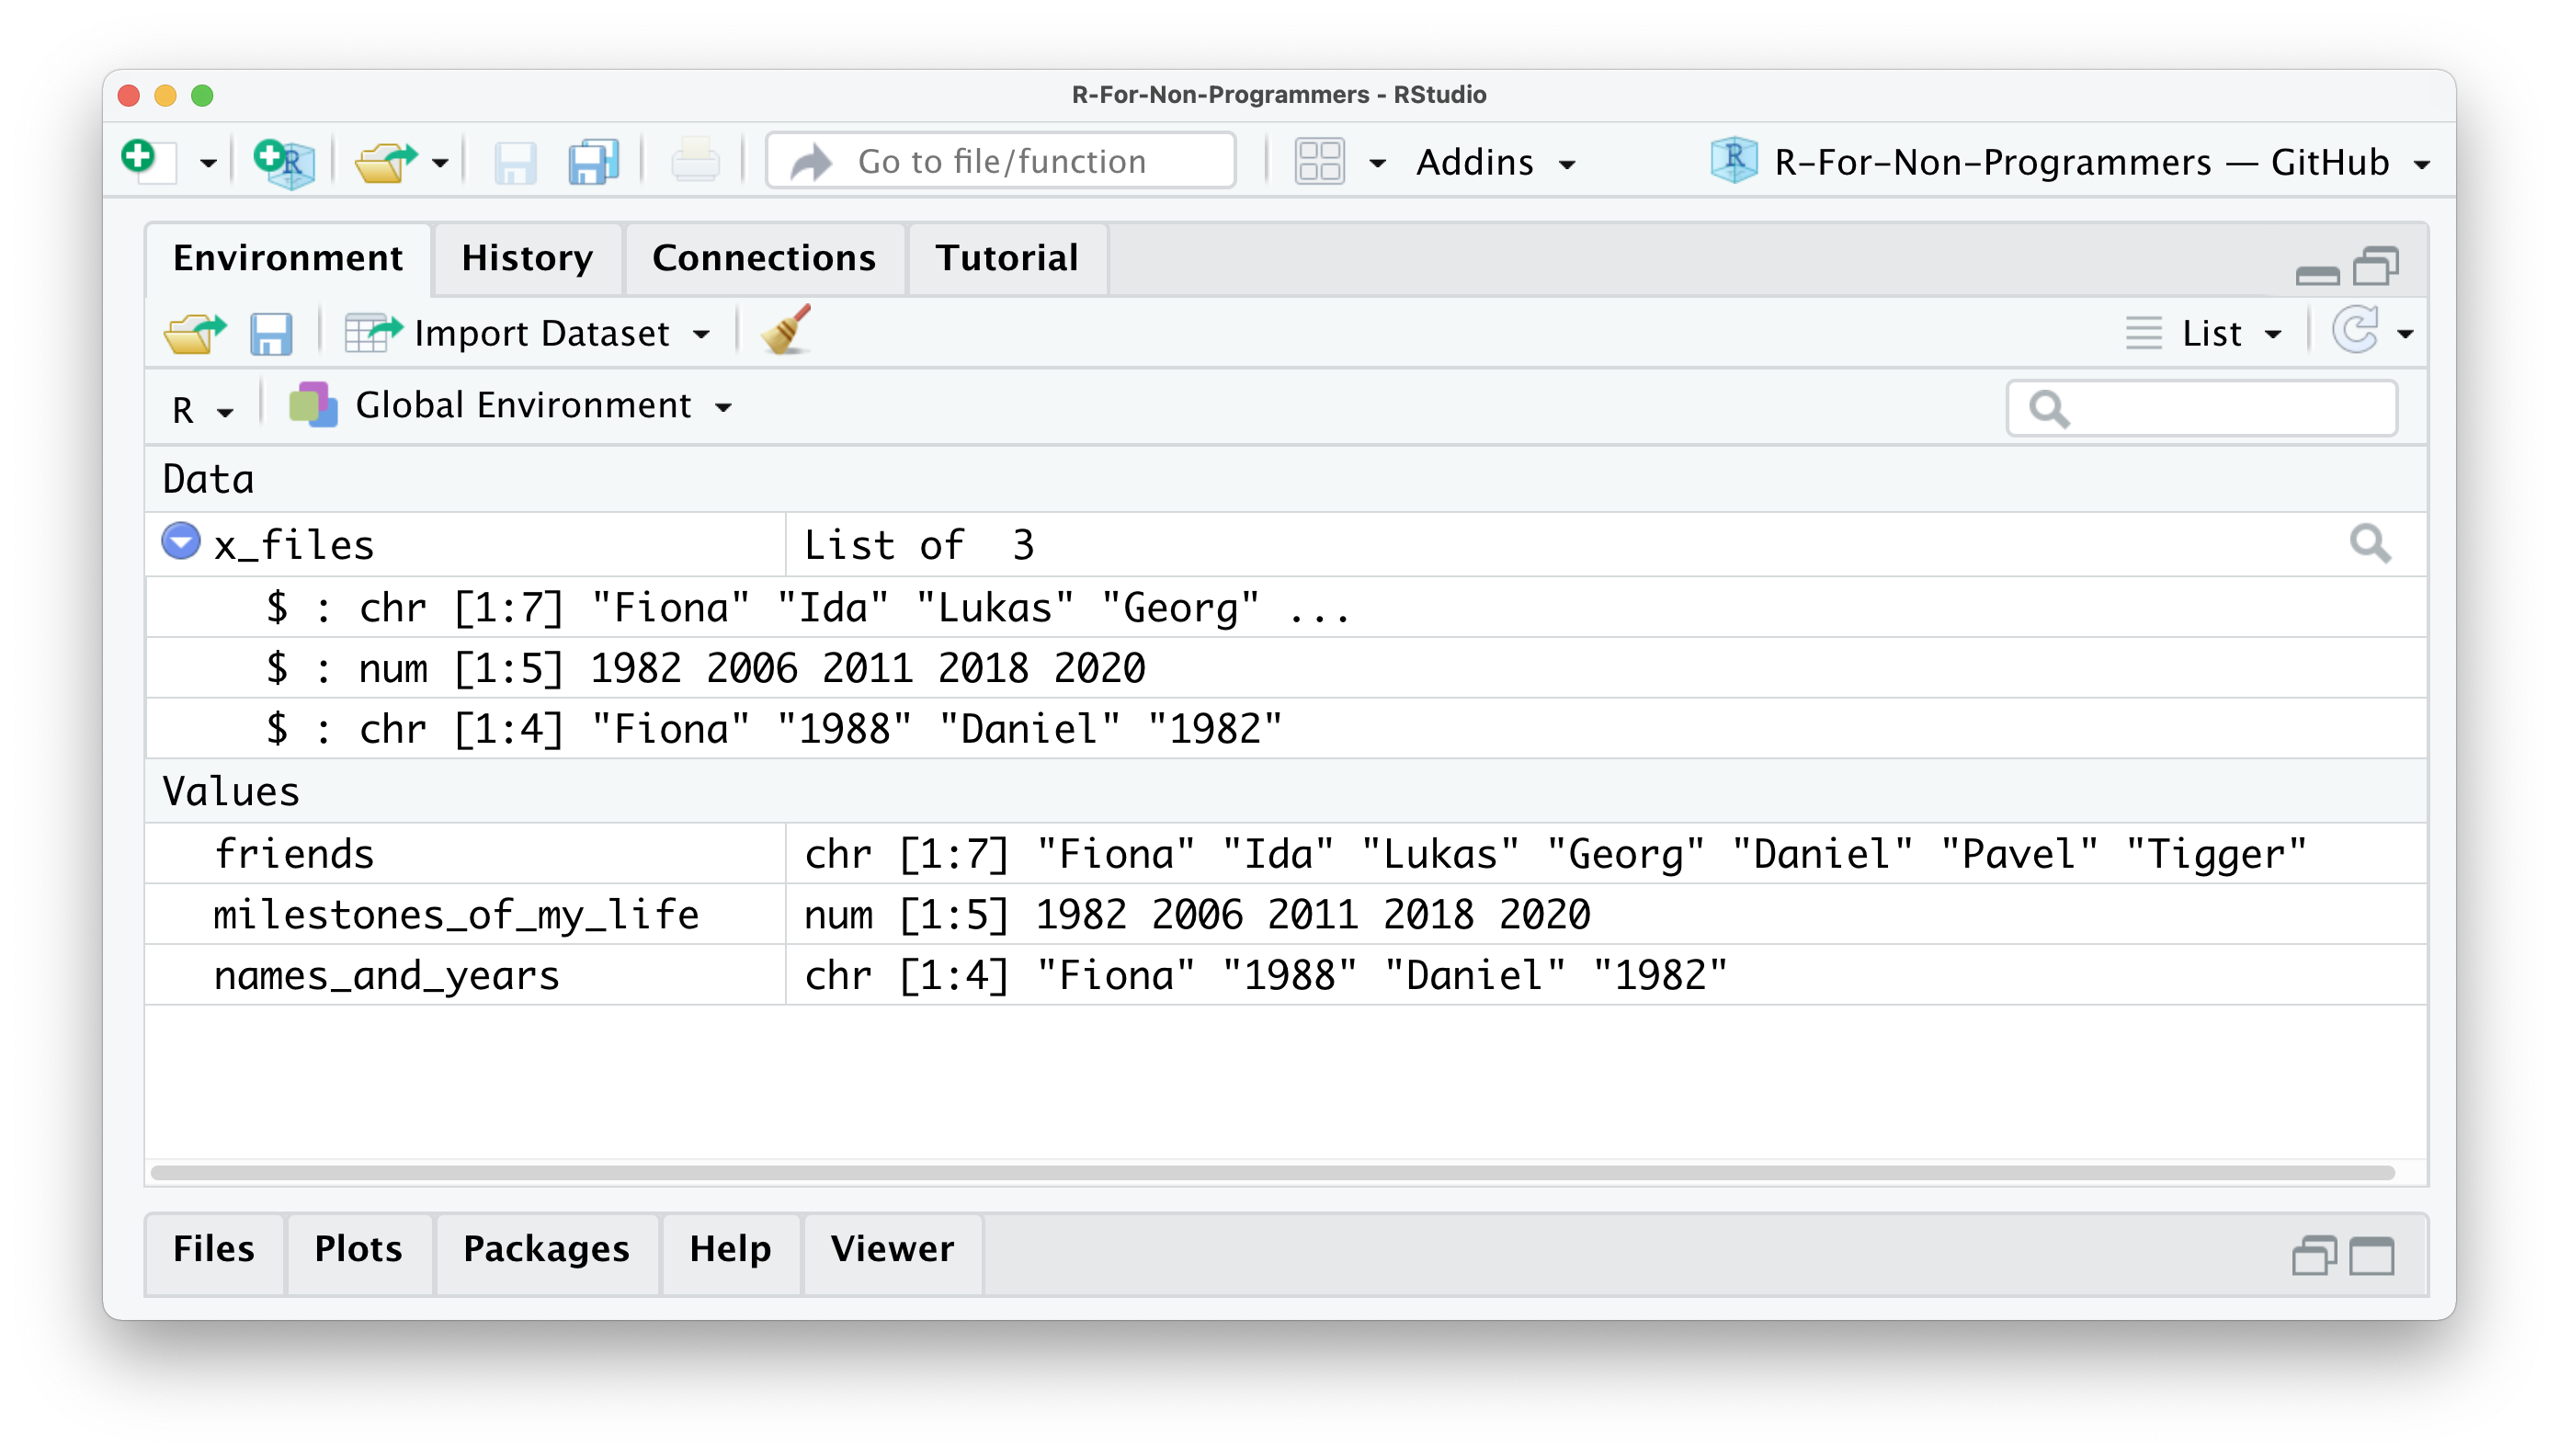
\includegraphics[width=38.67in]{images/chapter_05_img/02_basic_computation_environment_lists}

\}

\textbackslash caption\{The environment pane showing our objects and our list \texttt{x\_files}\}\label{fig:img-x-files}
\textbackslash end\{figure\}

In Chapter \ref{basic-computations-in-r}, I mentioned that we should avoid using the \texttt{=} operator and explained that it is used to assign values to objects. You can, if you want, use \texttt{=} instead of \texttt{\textless{}-}. They fulfil the same purpose. However, as mentioned before, it is not wise to do so. Here is an example that shows that, in principle, it is possible.

\begin{Shaded}
\begin{Highlighting}[]
\CommentTok{\# DO}
\NormalTok{(avengers1 }\OtherTok{\textless{}{-}} \FunctionTok{c}\NormalTok{(}\StringTok{"Iron Man"}\NormalTok{, }\StringTok{"Captain America"}\NormalTok{, }\StringTok{"Black Widow"}\NormalTok{, }\StringTok{"Vision"}\NormalTok{))}
\DocumentationTok{\#\# [1] "Iron Man"        "Captain America" "Black Widow"     "Vision"}
\CommentTok{\# DON\textquotesingle{}T}
\NormalTok{(}\AttributeTok{avengers2 =} \FunctionTok{c}\NormalTok{(}\StringTok{"Iron Man"}\NormalTok{, }\StringTok{"Captain America"}\NormalTok{, }\StringTok{"Black Widow"}\NormalTok{, }\StringTok{"Vision"}\NormalTok{))}
\DocumentationTok{\#\# [1] "Iron Man"        "Captain America" "Black Widow"     "Vision"}
\end{Highlighting}
\end{Shaded}

On a final note, naming your objects is limited. You cannot chose any name. First, every name needs to start with a letter. Second, you can only use letters, numbers \texttt{\_} and \texttt{.} as valid components of the names for your objects \citep[see also][Chapter 4.2.]{wickham2016r}. I recommend to establish a naming convention that you adhere to. Personally I prefer to only user lower letters and \texttt{\_} to separate/connect words. You want to keep names informative, succinct and precise. Here are some examples of what some might consider good and bad choices for names.

\begin{Shaded}
\begin{Highlighting}[]
\CommentTok{\# Good choices}
\NormalTok{income\_per\_annum}
\NormalTok{open\_to\_exp          }\CommentTok{\# for \textquotesingle{}openness to new experiences\textquotesingle{}}
\NormalTok{soc\_int              }\CommentTok{\# for \textquotesingle{}social integration\textquotesingle{}}
 
\CommentTok{\# Bad choices}
\NormalTok{IncomePerAnnum}
\NormalTok{measurement\_of\_boredom\_of\_watching\_youtube}
\NormalTok{Sleep.per\_monthsIn.hours}
\end{Highlighting}
\end{Shaded}

Ultimately, you need to be able to effectively work with your data and output. Ideally, this should be true for others as well who want or need to work with your R project as well, e.g.~your co-investigator or supervisor. The same is true for your column names in datasets (see Chapter @ref()). Some more information about coding style (i.e.~the style of writing coding) can be found in Chapter \ref{coding-etiquette}.

\hypertarget{functions}{%
\section{Functions}\label{functions}}

I used the term `function' multiple times, but I never thoroughly explained what they are and why we need them. In simple terms, functions are objects. They contain lines of code that someone has written for us or we have written ourselves. One could say they are code snippets ready to use. Someone else might see them as shortcuts for our programming. Functions increase the speed with which we perform our analysis and write our computations and make our code more readable. Consider computing the \texttt{mean} of values stored in the object \texttt{pocket\_money}.

\begin{Shaded}
\begin{Highlighting}[]
\CommentTok{\# First we create an object that stores our desired values}
\NormalTok{pocket\_money }\OtherTok{\textless{}{-}} \FunctionTok{c}\NormalTok{(}\DecValTok{0}\NormalTok{, }\DecValTok{1}\NormalTok{, }\DecValTok{1}\NormalTok{, }\DecValTok{2}\NormalTok{, }\DecValTok{3}\NormalTok{, }\DecValTok{5}\NormalTok{, }\DecValTok{8}\NormalTok{, }\DecValTok{13}\NormalTok{, }\DecValTok{21}\NormalTok{, }\DecValTok{34}\NormalTok{, }\DecValTok{55}\NormalTok{, }\DecValTok{89}\NormalTok{)}

\CommentTok{\#1 Manually compute the mean}
\NormalTok{sum }\OtherTok{\textless{}{-}} \DecValTok{0} \SpecialCharTok{+} \DecValTok{1} \SpecialCharTok{+} \DecValTok{1} \SpecialCharTok{+} \DecValTok{2} \SpecialCharTok{+} \DecValTok{3} \SpecialCharTok{+} \DecValTok{5} \SpecialCharTok{+} \DecValTok{8} \SpecialCharTok{+} \DecValTok{13} \SpecialCharTok{+} \DecValTok{21} \SpecialCharTok{+} \DecValTok{34} \SpecialCharTok{+} \DecValTok{55} \SpecialCharTok{+} \DecValTok{89}
\NormalTok{sum }\SpecialCharTok{/} \DecValTok{12} \CommentTok{\# There are 12 items in the object}
\DocumentationTok{\#\# [1] 19.33333}
\CommentTok{\#2 Use a function to compute the mean}
\FunctionTok{mean}\NormalTok{(pocket\_money)}
\DocumentationTok{\#\# [1] 19.33333}
\CommentTok{\#3 Let\textquotesingle{}s make sure \#1 and \#2 are actually the same}
\NormalTok{sum }\SpecialCharTok{/} \DecValTok{12} \SpecialCharTok{==} \FunctionTok{mean}\NormalTok{(pocket\_money)}
\DocumentationTok{\#\# [1] TRUE}
\end{Highlighting}
\end{Shaded}

If we manually compute the mean, we first calculate the sum of all values in the object \texttt{pocket\_money}\footnote{If you find the order of numbers suspicious, it is because it represents the famous \href{https://en.wikipedia.org/wiki/Fibonacci_number}{Fibonacci sequence}.}. Then we divide it by the number of values in the object, which is \texttt{12}. This is the traditional way of computing the mean as we know it from primary school. However, by simply using the function \texttt{mean()}, we not only write considerably less code, but it is also much easier to understand as well because the word \texttt{mean} does precisely what we would expect. Which one do you find easier?

To further illustrate how functions look like, let's create one ourselves and call it \texttt{my\_mean}.

\begin{Shaded}
\begin{Highlighting}[]
\NormalTok{my\_mean }\OtherTok{\textless{}{-}} \ControlFlowTok{function}\NormalTok{(numbers)\{}
\NormalTok{  sum }\OtherTok{\textless{}{-}} \FunctionTok{sum}\NormalTok{(numbers)              }\CommentTok{\# Compute the sum of all values in \textquotesingle{}numbers\textquotesingle{}}
\NormalTok{  result }\OtherTok{\textless{}{-}}\NormalTok{ sum}\SpecialCharTok{/}\FunctionTok{length}\NormalTok{(numbers)    }\CommentTok{\# Divide the sum by the number of items in \textquotesingle{}numbers\textquotesingle{}}
  \FunctionTok{return}\NormalTok{(result)                   }\CommentTok{\# Return the result in the console}
\NormalTok{\}}

\FunctionTok{my\_mean}\NormalTok{(pocket\_money)}
\DocumentationTok{\#\# [1] 19.33333}
\end{Highlighting}
\end{Shaded}

Do not worry if half of this code does not make sense to you. Writing functions is an advanced R skill. However, it is good to know how functions look on the `inside'. You certainly can see the similarities between the code we have written before, but instead of using actual numbers, we work with placeholders like \texttt{numbers}. This way, we can use a function for different data and do not have to rewrite it every time.

All functions in R share the same structure. They have a \texttt{name} followed by \texttt{()}. Within these parentheses, we put \texttt{arguments}, which have specific \texttt{values}. For example, a function would look something like this:

\begin{Shaded}
\begin{Highlighting}[]
\FunctionTok{name\_of\_function}\NormalTok{(}\AttributeTok{argument\_1 =}\NormalTok{ value\_1,}
                 \AttributeTok{argument\_2 =}\NormalTok{ value\_2,}
                 \AttributeTok{argument\_3 =}\NormalTok{ value\_3)}
\end{Highlighting}
\end{Shaded}

How many arguments there are and what kind of values you can provide is very much dependent on the function you use. Thus, not every function takes every value. In the case of \texttt{mean()}, the function takes an object which holds a sequence of \texttt{numeric} values. It would make very little sense to compute the mean of our \texttt{friends} object, because it only contains names. R would return an error message:

\begin{Shaded}
\begin{Highlighting}[]
\FunctionTok{mean}\NormalTok{(friends)}
\DocumentationTok{\#\# Warning in mean.default(friends): argument is not numeric or logical: returning}
\DocumentationTok{\#\# NA}
\DocumentationTok{\#\# [1] NA}
\end{Highlighting}
\end{Shaded}

\texttt{NA} refers to a value that is \emph{`not available'}. In this case, R tries to compute the mean, but the result is not available, because the values are not \texttt{numeric} but a \texttt{character}. In your dataset, you might find cells that are \texttt{NA}, which means there is data missing. Remember: If a function attempts a computation that includes even just a single value that is \texttt{NA}, R will return \texttt{NA}. However, there is a way to fix this. You will learn more about how to deal with \texttt{NA} values in Chapter @ref().

Sometimes you will also get a message from R that states \texttt{NaN}. \texttt{NaN} stands for \emph{`not a number'} and is returned when something is not possible to compute, for example:

\begin{Shaded}
\begin{Highlighting}[]
\CommentTok{\# Example 1}
\DecValTok{0}\SpecialCharTok{/}\DecValTok{0}
\DocumentationTok{\#\# [1] NaN}
\CommentTok{\# Example 2}
\FunctionTok{sqrt}\NormalTok{(}\SpecialCharTok{{-}}\DecValTok{9}\NormalTok{)}
\DocumentationTok{\#\# Warning in sqrt({-}9): NaNs produced}
\DocumentationTok{\#\# [1] NaN}
\end{Highlighting}
\end{Shaded}

\hypertarget{r-packages}{%
\section{R packages}\label{r-packages}}

R has many built-in functions that we can use right away. However, some of the most interesting ones are developed by different programmers, data scientists and enthusiasts. To add more functions to your repertoire, you can install R packages. R packages are a collection of functions that you can download and use for your own analysis. Throughout this book, you will learn about and use many different R packages to accomplish various tasks.

To give you another analogy,

\begin{itemize}
\item
  R is like a global supermarket,
\item
  RStudio is like my shopping cart,
\item
  and R packages are the products I can pick from the shelves.
\end{itemize}

Luckily, R packages are free to use, so I do not have to bring my credit card. For me, these additional functions, developed by some of the most outstanding scientists, is what keeps me addicted to performing my research in R.

R packages do not only include functions but often include datasets and documentation of what each function does. This way, you can easily try every function right away, even without your own dataset and read through what each function in the package does. Figure \ref{fig:img-r-package-documentation}

\begin{figure}

{\centering 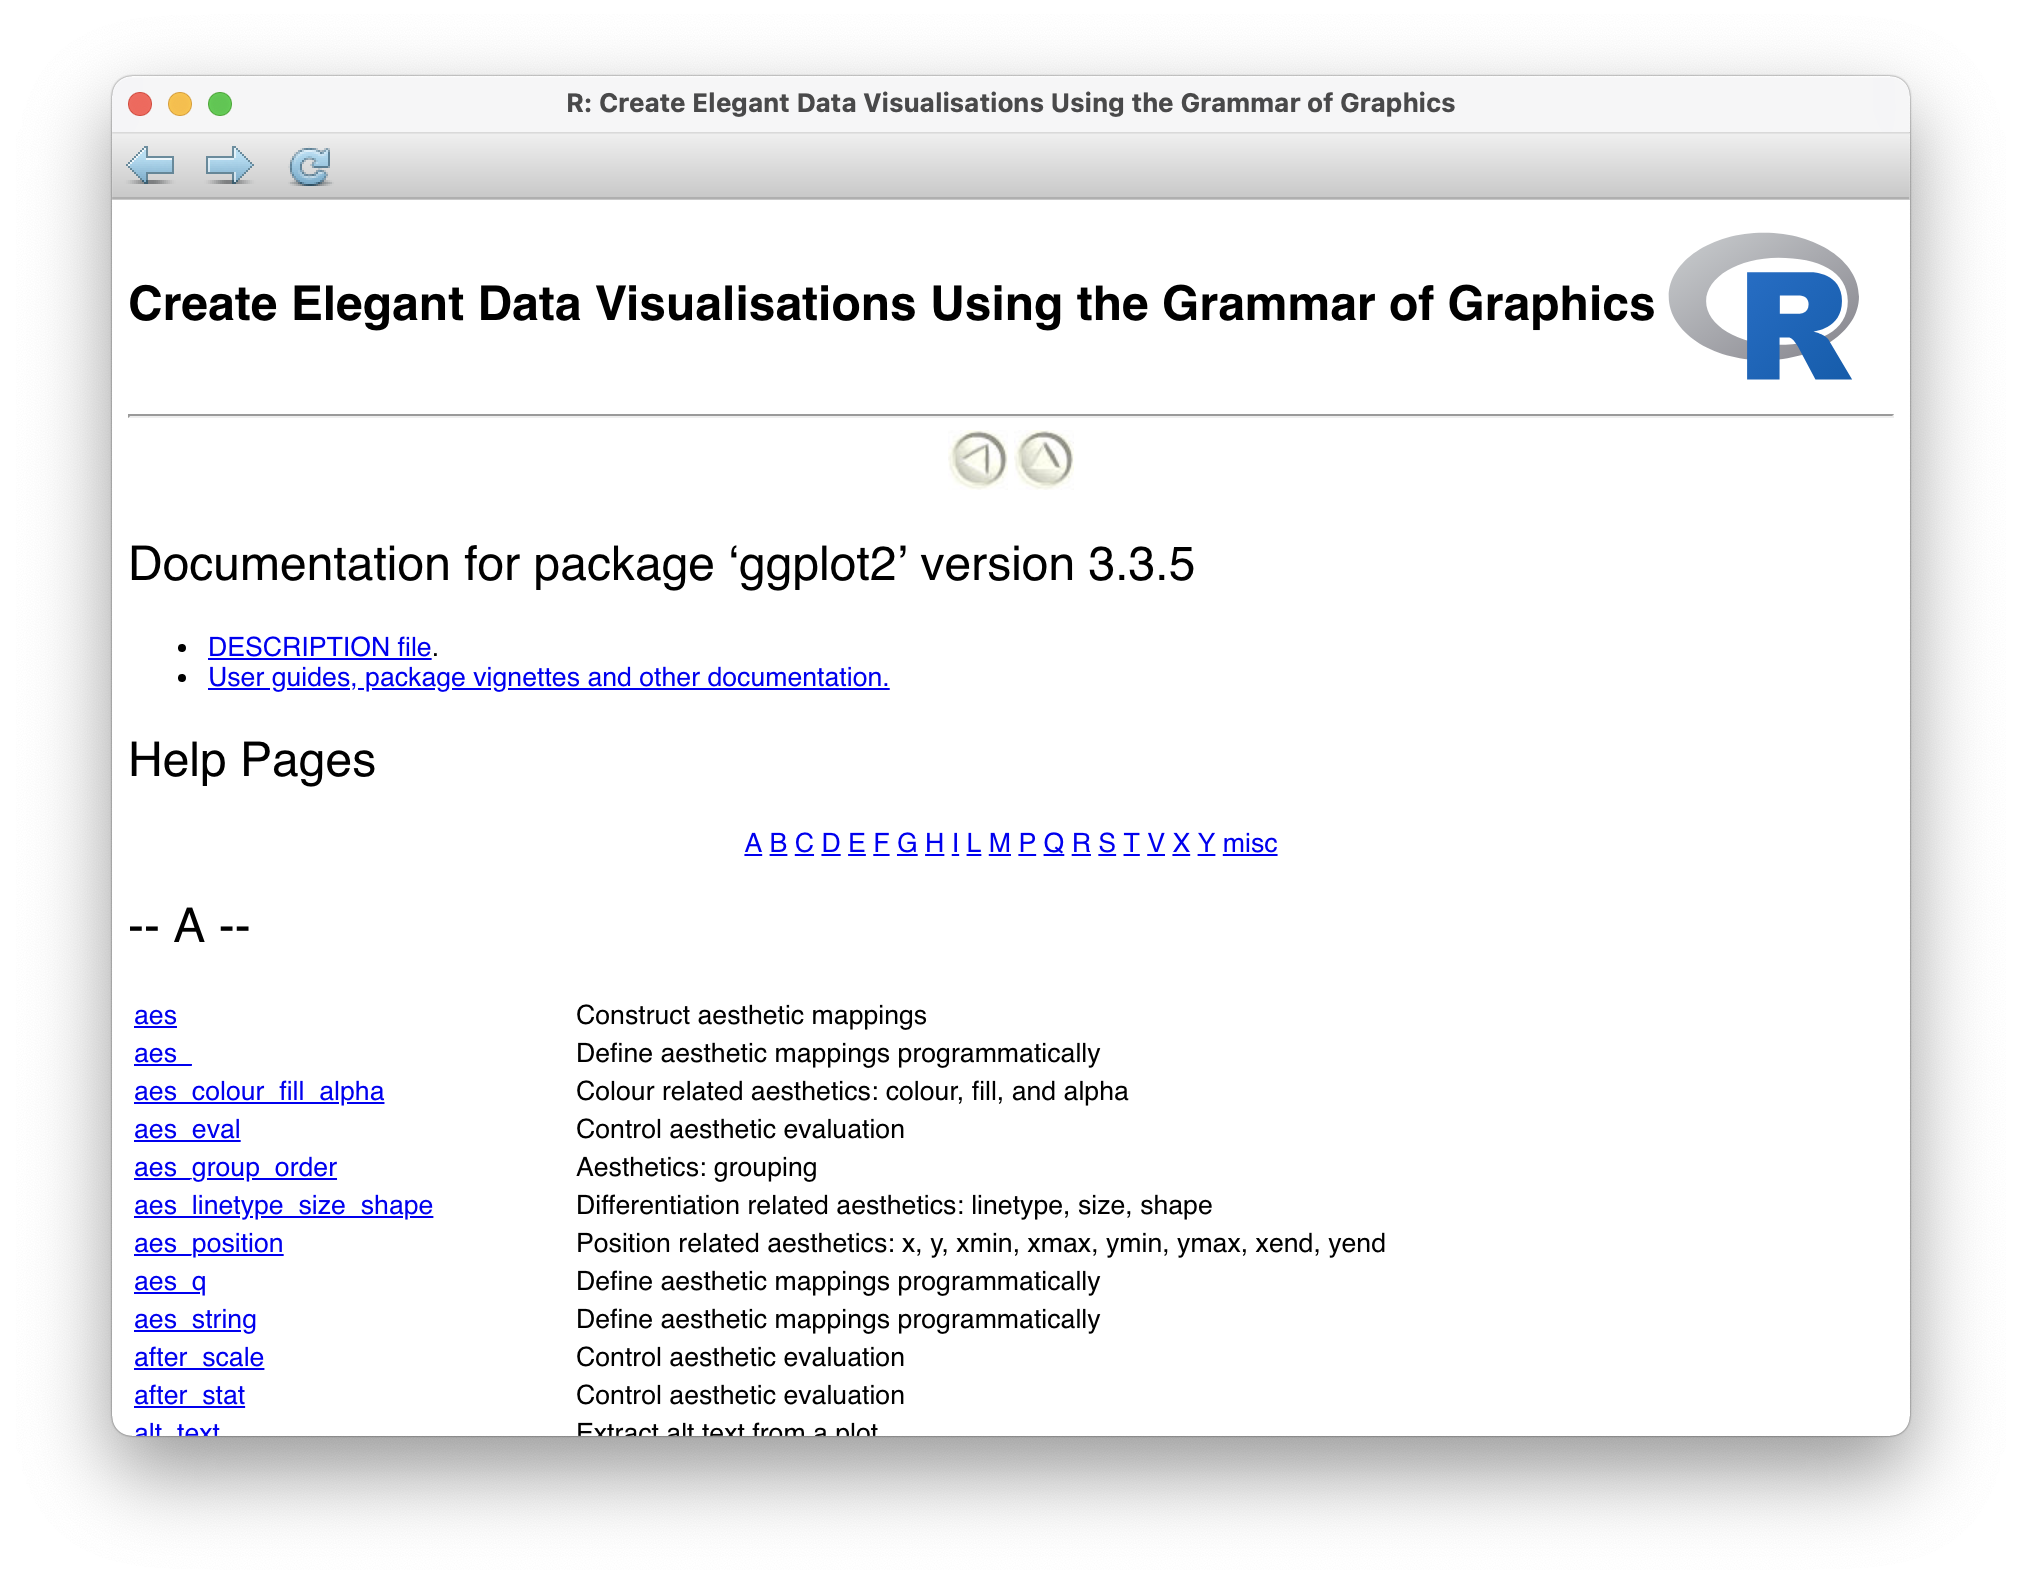
\includegraphics[width=28.08in]{images/chapter_05_img/r_package_documentation} 

}

\caption{The R package documentation for 'ggplot2'}\label{fig:img-r-package-documentation}
\end{figure}

However, how do you find those R packages? They are right at your fingertips. You have two options:

\begin{enumerate}
\def\labelenumi{\arabic{enumi}.}
\item
  Use the function \texttt{install.packages()}
\item
  Use the packages pane in RStudio (see Chapter \ref{the-files-plots-packages-help-viewer-window})
\end{enumerate}

\hypertarget{installing-packages-using-a-function}{%
\subsection{\texorpdfstring{Installing packages using \texttt{install.packages()}}{Installing packages using install.packages()}}\label{installing-packages-using-a-function}}

The simplest and fastest way to install a package is calling the function \texttt{install.packages()}. You can either use it to install a single package or install a series of packages all at once using our trusty \texttt{c()} function. All you need to know is the name of the package. This approach works for all packages that are on CRAN (remember CRAN from Chapter \ref{installing-r}?).

\begin{Shaded}
\begin{Highlighting}[]
\CommentTok{\# Install a single package}
\FunctionTok{install.packages}\NormalTok{(}\StringTok{"tidyverse"}\NormalTok{)}

\CommentTok{\# Install multiple packages at once}
\FunctionTok{install.packages}\NormalTok{(}\FunctionTok{c}\NormalTok{(}\StringTok{"tidyverse"}\NormalTok{, }\StringTok{"naniar"}\NormalTok{, }\StringTok{"psych"}\NormalTok{))}
\end{Highlighting}
\end{Shaded}

If a package is not available from CRAN, chances are you can find them on \href{https://github.com}{GitHub}. GitHub is probably the world's largest global platform for programmers from all walks of life, and many of them develop fantastic R packages that make R programming not just easier but a lot more fun. As you continue to work in R, you should seriously consider creating your own account to keep backups of your R projects (see also Chapter \ref{next-steps-github}).

An essential companion for this book is \texttt{r4np}, which contains all datasets for this book and some useful functions to get you up and running in no time.

\begin{Shaded}
\begin{Highlighting}[]
\CommentTok{\# Install the \textquotesingle{}r4np\textquotesingle{} pacakge from GitHub}
\NormalTok{devtools}\SpecialCharTok{::}\FunctionTok{install\_github}\NormalTok{(}\StringTok{"ddauber/r4np"}\NormalTok{)}
\end{Highlighting}
\end{Shaded}

\hypertarget{installing-packages-via-rstudio}{%
\subsection{Installing packages via RStudio's package pane}\label{installing-packages-via-rstudio}}

RStudio offers a very convenient way of installing packages. In the packages pane, you cannot only see your installed packages, but you have two more buttons: \texttt{Install} and \texttt{Update}. The names are very self-explanatory. To install an R package you can follow the following steps:

\begin{enumerate}
\def\labelenumi{\arabic{enumi}.}
\item
  Click on \texttt{Install}.
\item
  In most cases, you want to make sure you have \texttt{Repository\ (CRAN)} selected.

  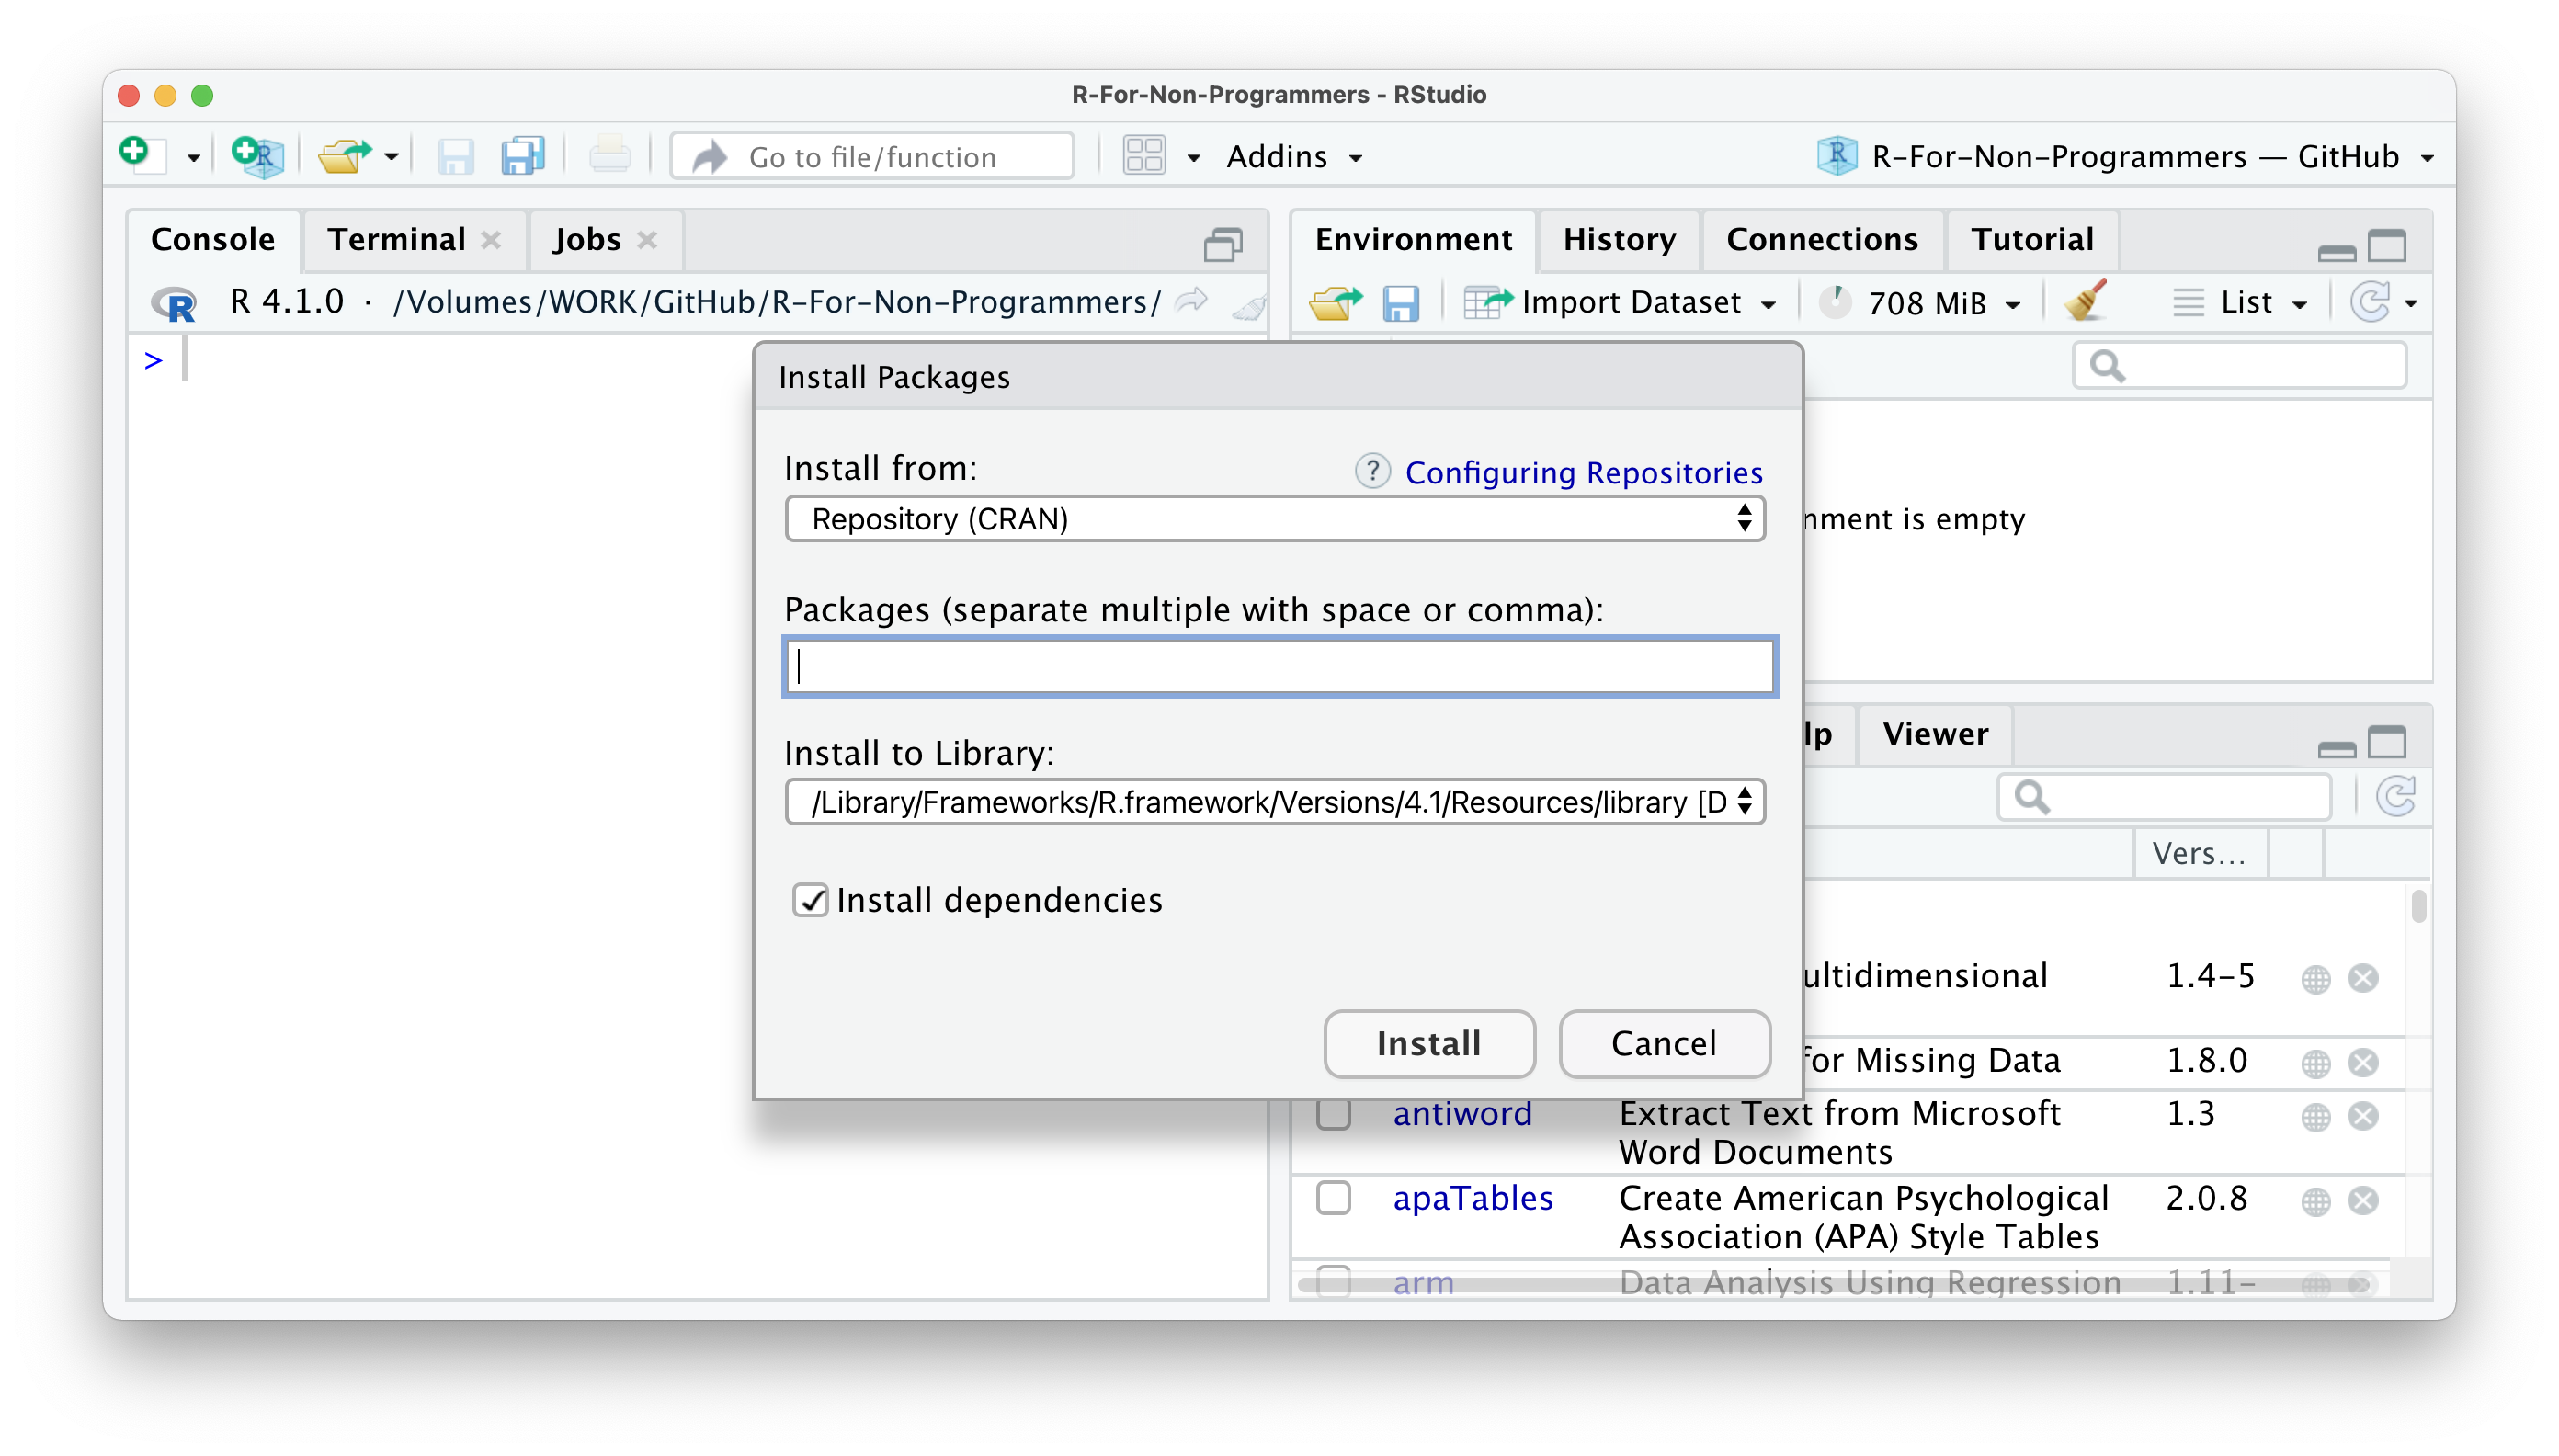
\includegraphics{images/chapter_05_img/install_r_packages/01_install_r_packages.png}
\item
  Type in the name of the package you wish to install. RStudio offers an auto-complete feature to make it even easier to find the package you want.

  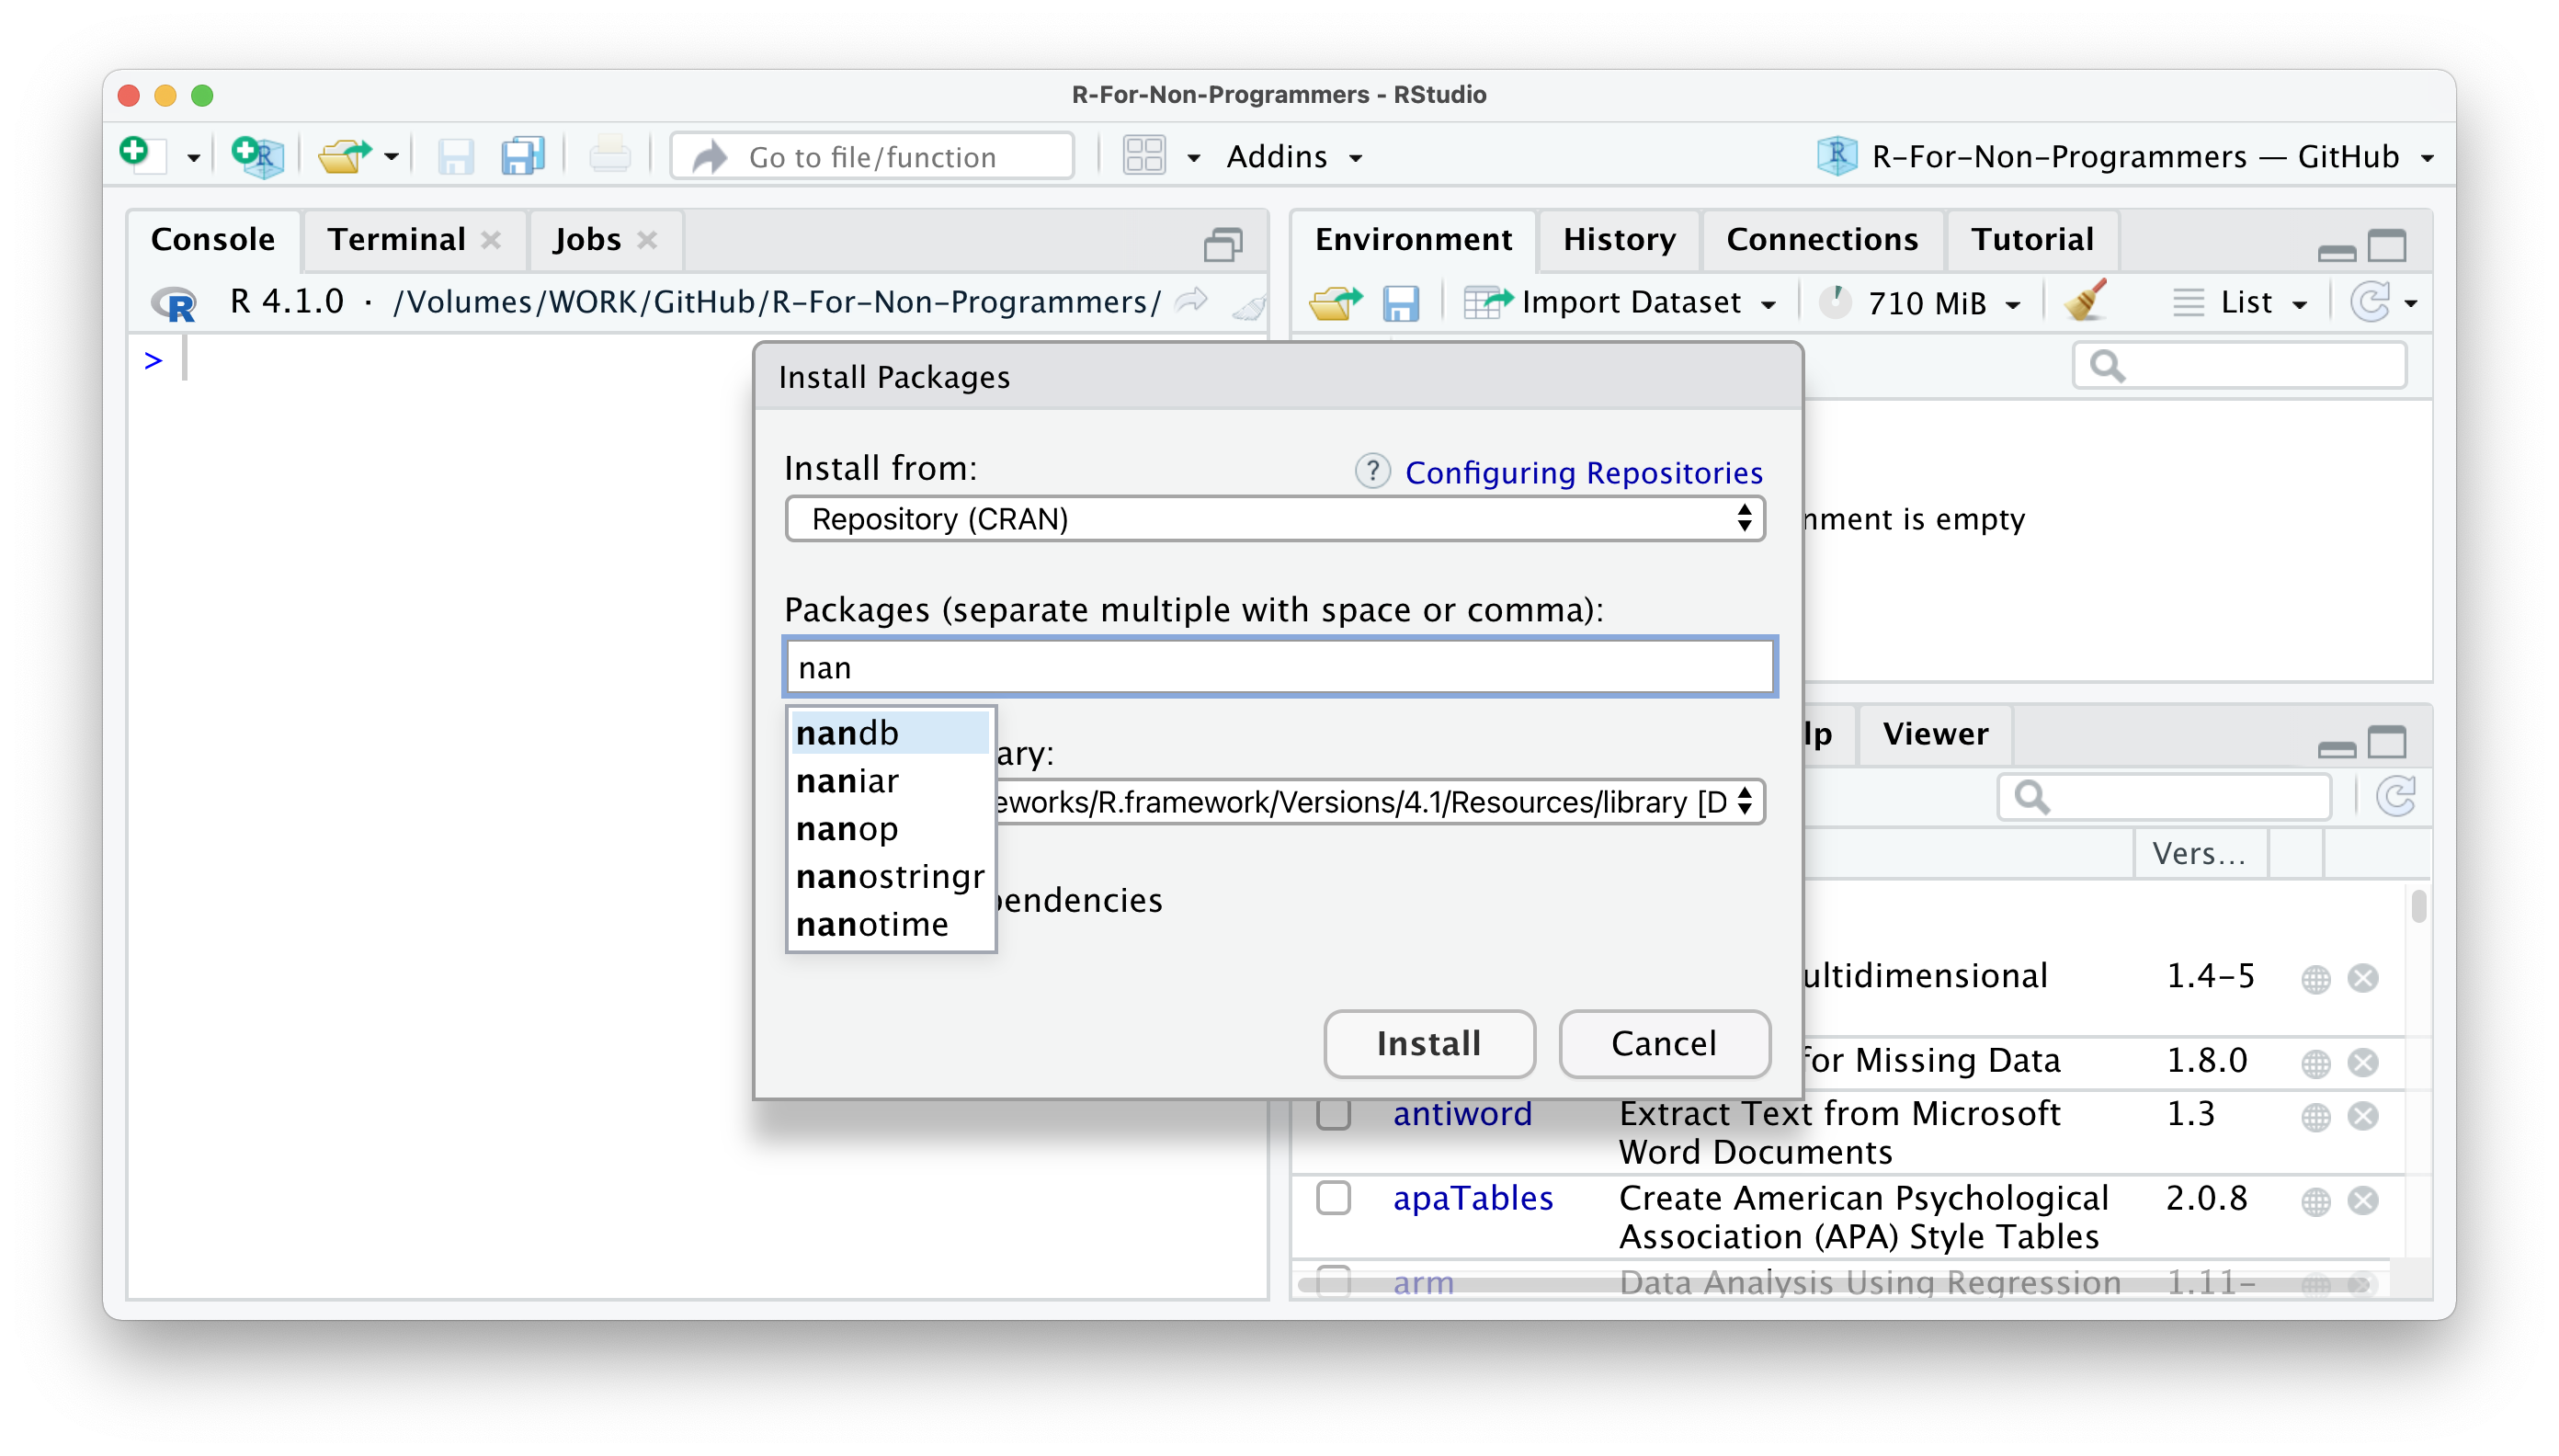
\includegraphics{images/chapter_05_img/install_r_packages/02_install_r_packages.png}
\item
  I recommend NOT to change the option which says \texttt{Install\ to\ library.} The default library settings will suffice.
\item
  Finally, I recommend to select \texttt{Install\ dependencies}, because some packages need other packages to function properly. This way, you do not have to do this manually.

  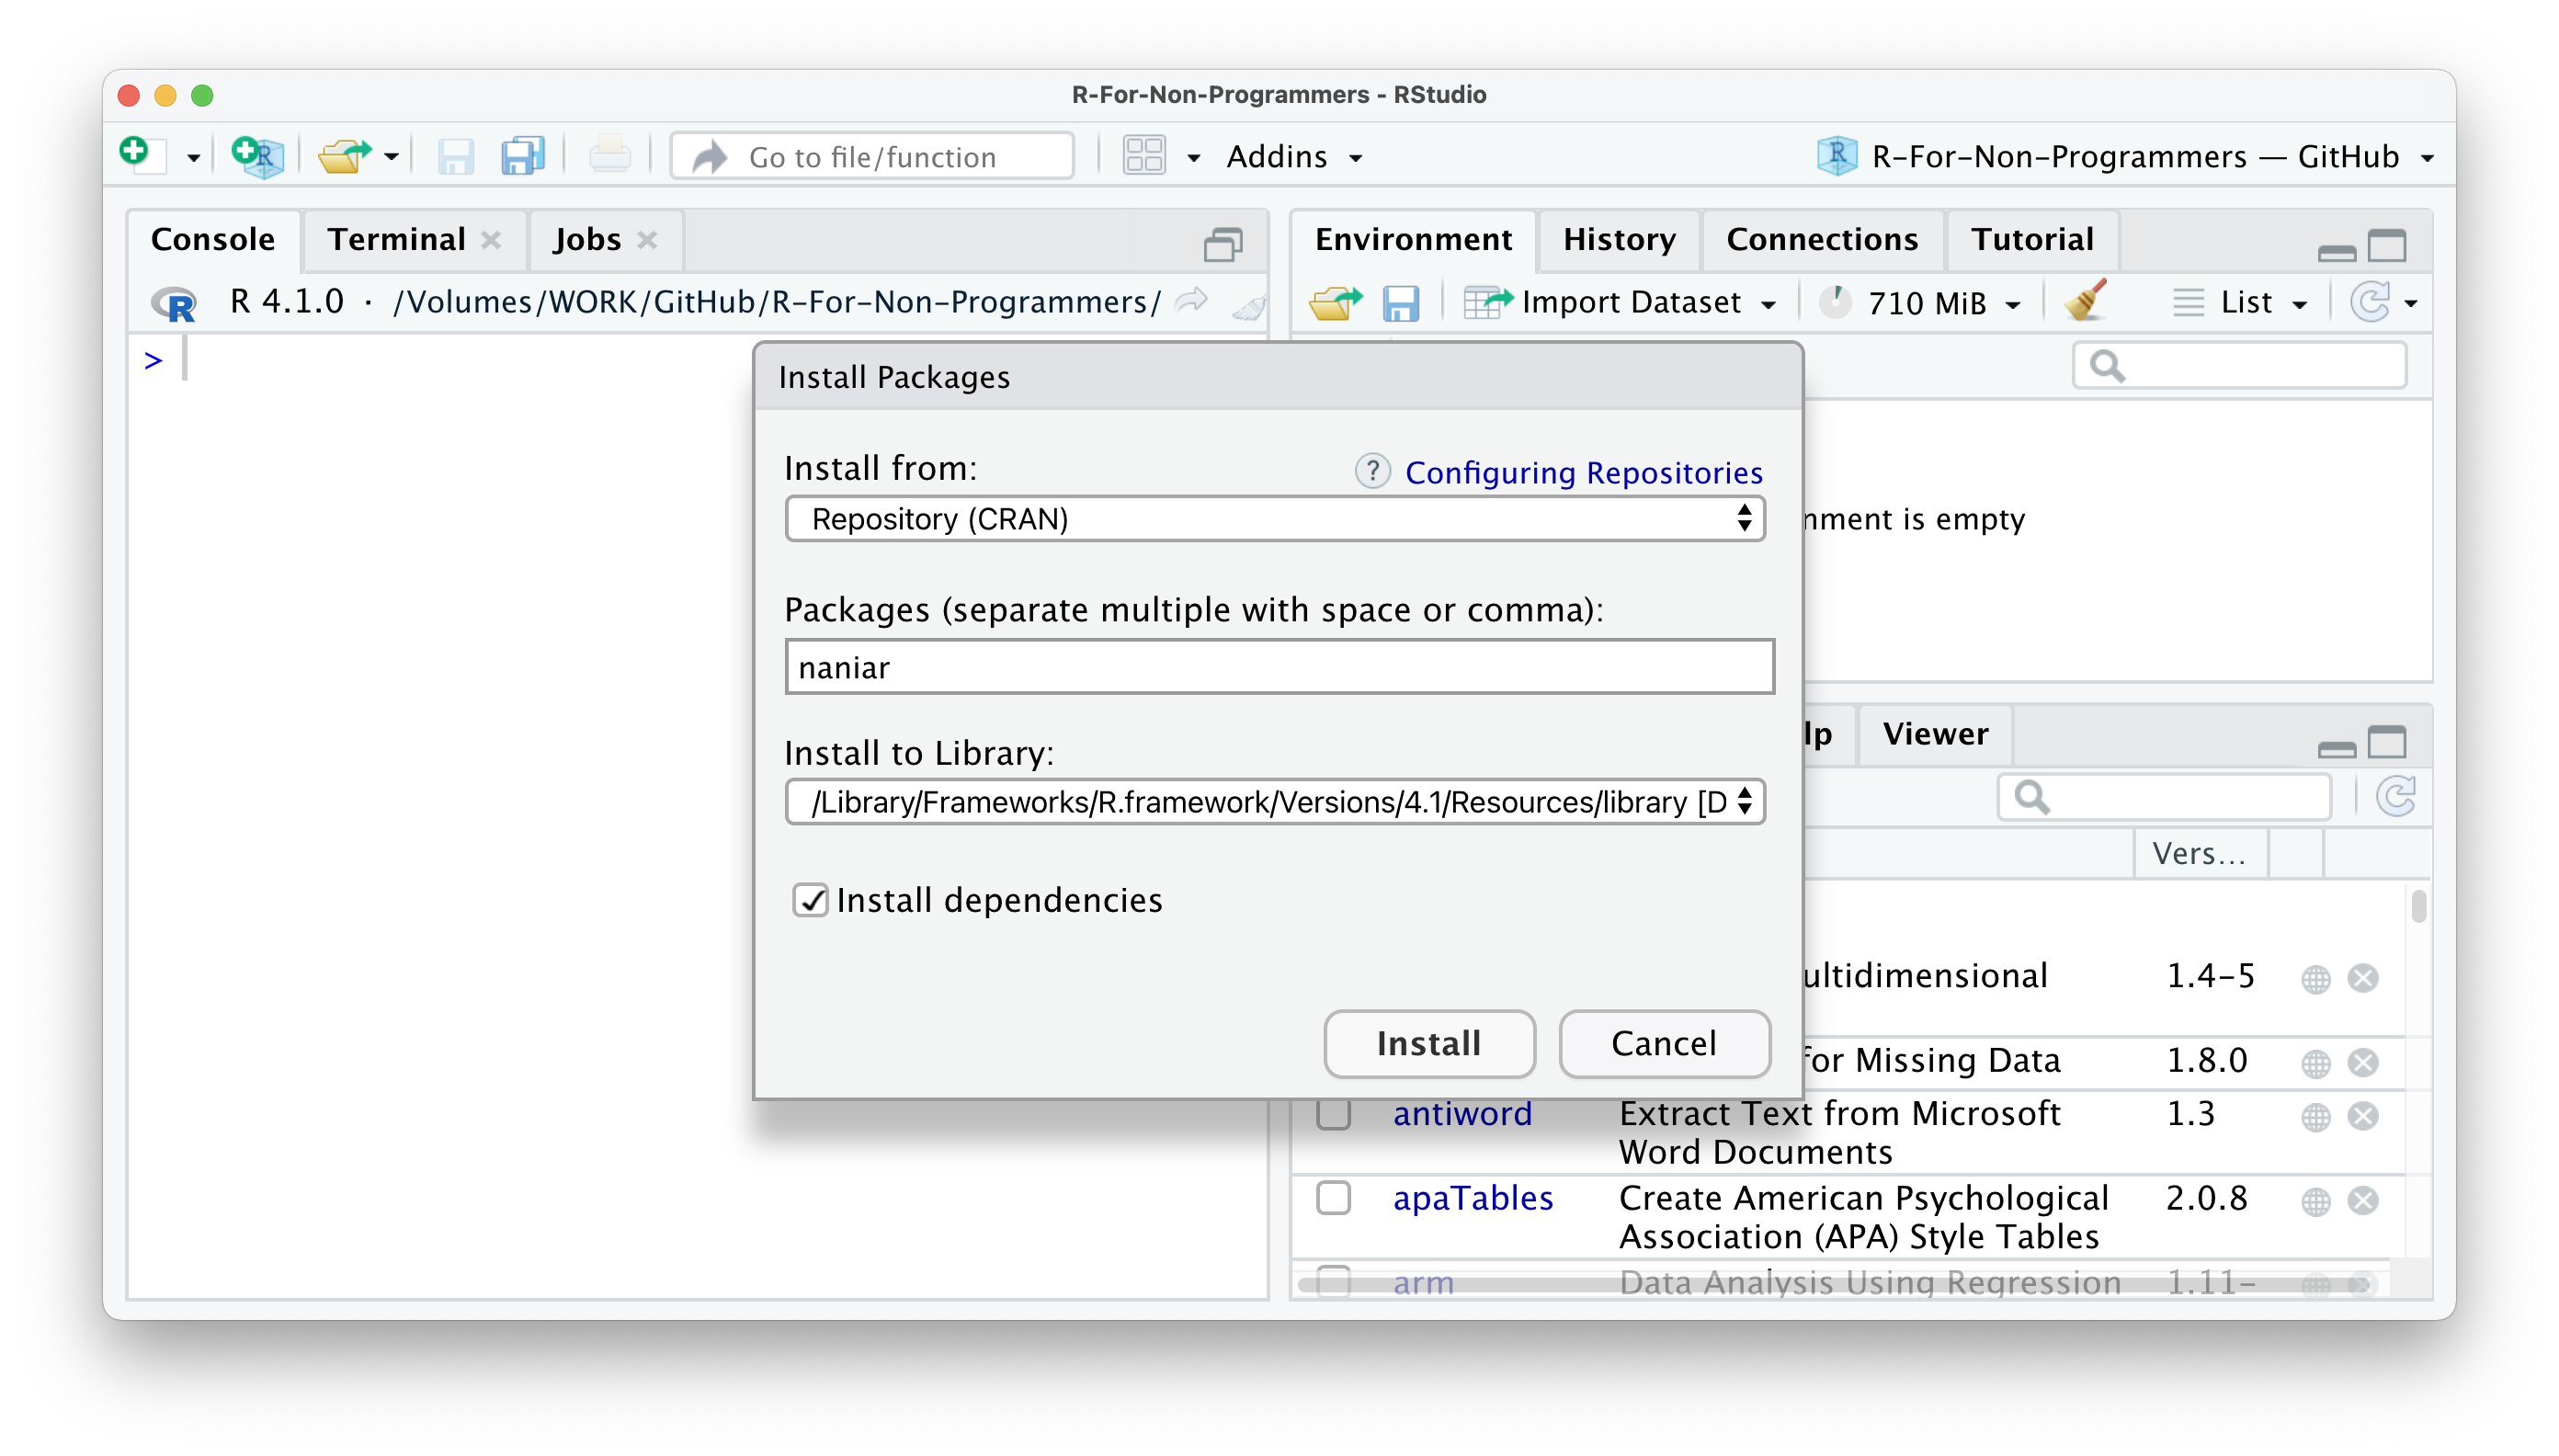
\includegraphics{images/chapter_05_img/install_r_packages/03_install_r_packages.png}
\end{enumerate}

The only real downside of using the packages pane is that you cannot install packages hosted on GitHub only. However, you can download them from there and install them directly from your computer using this option. This is particularly useful if you do not have an internet connection but you already downloaded the required packages onto a hard drive.

\hypertarget{using-r-packages}{%
\subsection{Using R Packages}\label{using-r-packages}}

Now that you have a nice collection of R packages, the next step would be to use them. While you only have to install R packages once, you have to `activate' them every time you start an new session in RStudio. This process is also called `loading an R package'. Once an R package is loaded, you can use all its functions. To load an R package, we have to use the function \texttt{library()}.

\begin{Shaded}
\begin{Highlighting}[]
\FunctionTok{library}\NormalTok{(tidyverse)}
\end{Highlighting}
\end{Shaded}

The \texttt{tidyverse} package is a special kind of package. It contains multiple packages and loads them all at once. Almost all included packages (and more) you will use at some point when working through this book.

I know what you are thinking. Can you use \texttt{c()} to load all your packages at once? Unfortunately not. However, there is a way to do this, but it goes beyond the scope of this book to fully explain this (if you are curious, you can take a peek \href{https://stackoverflow.com/questions/8175912/load-multiple-packages-at-once}{here}).

Besides, it is not always advisable to load all functions of an entire package. One reason could be that two packages contain a function with the same name but with a different purpose. Two functions with the same name create a conflict between these two packages, and one of the functions would not be usable. Another reason could be that you only need to use the function once, and loading the whole package to use only one specific function seems excessive. Instead, you can explicitly call functions from packages without loading the package. For example, we might want to use the \texttt{vismis()} function from the \texttt{naniar} package to show where data is missing in our dataset \texttt{airquality}. Writing the code this way is also much quicker than loading the package and then calling the function if you don't use it repeatedly. Copy the code and try it yourself. Make sure you have \texttt{naniar} installed (see \protect\hyperlink{install-packages-tidyverse-nanair-psych}{above}). We will work with this package when we explore missing data in Chapter @ref().

\begin{Shaded}
\begin{Highlighting}[]
\CommentTok{\# Here I use the dataset \textquotesingle{}airquality\textquotesingle{}, which comes with R}
\NormalTok{naniar}\SpecialCharTok{::}\FunctionTok{vis\_miss}\NormalTok{(airquality)}
\end{Highlighting}
\end{Shaded}

\begin{center}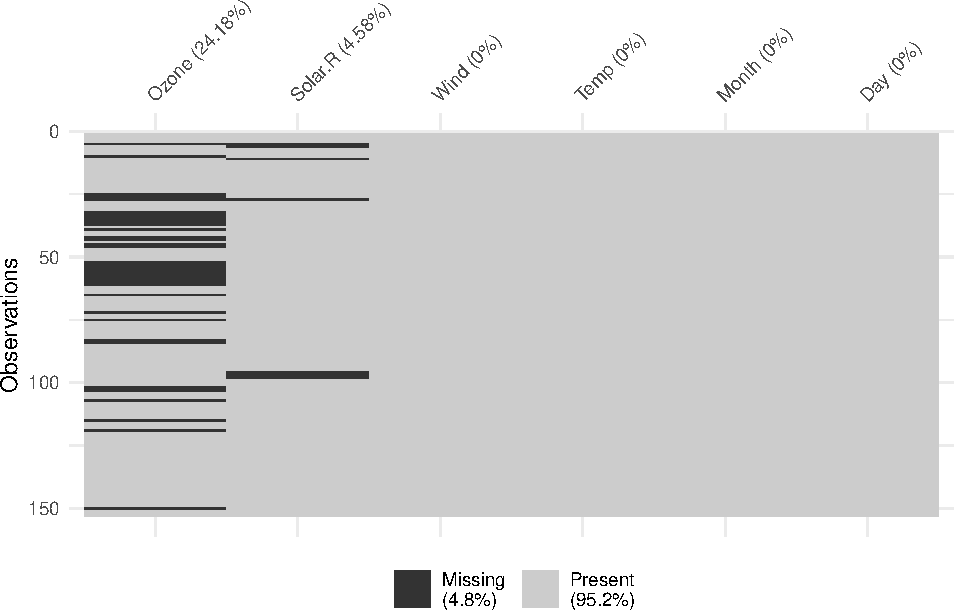
\includegraphics{r_for_non_programmers_files/figure-latex/Explicitly calling functions from R packages-1} \end{center}

\hypertarget{coding-etiquette}{%
\section{Coding etiquette}\label{coding-etiquette}}

Now you know everything to get started, but before we jump into our first project, I would like to briefly touch upon coding etiquette. This is not something that improves your analytical or coding skills directly, but is essential in building good habbits and making your life and those of others a little easier. Consider writing code like growing plants in your garden. You want to nurture the good plants, remove the weed and add labels that tell you which plant it is that you are growing. At the end of the day, you want your garden to be well-maintained. Treat you programming code the same way.

A script (see Chapter @ref()) with code should always have at least the following qualities:

\begin{itemize}
\item
  Only contains code that is necessary,
\item
  Is easy to read and understand,
\item
  Is self-contained.
\end{itemize}

With simple code this is easily achieved. However, what about more complex and longer code representing a whole set of analytical steps?

\begin{Shaded}
\begin{Highlighting}[]
\CommentTok{\# Very messy code}

\FunctionTok{library}\NormalTok{(tidyverse)}
\FunctionTok{library}\NormalTok{(jtools)}
\NormalTok{model1 }\OtherTok{\textless{}{-}} \FunctionTok{lm}\NormalTok{(covid\_cases\_per\_1m }\SpecialCharTok{\textasciitilde{}}\NormalTok{ idv, }\AttributeTok{data =}\NormalTok{ df)}
\FunctionTok{summ}\NormalTok{(model1, }\AttributeTok{scale =} \ConstantTok{TRUE}\NormalTok{, }\AttributeTok{transform.response =} \ConstantTok{TRUE}\NormalTok{, }\AttributeTok{vifs =} \ConstantTok{TRUE}\NormalTok{)}
\NormalTok{df }\SpecialCharTok{\%\textgreater{}\%} \FunctionTok{ggplot}\NormalTok{(}\FunctionTok{aes}\NormalTok{(covid\_cases\_per\_1m, idv, }\AttributeTok{colour =}\NormalTok{ europe, }\AttributeTok{label =}\NormalTok{ country))}\SpecialCharTok{+}
\FunctionTok{theme\_minimal}\NormalTok{()}\SpecialCharTok{+} \FunctionTok{geom\_label}\NormalTok{(}\AttributeTok{nudge\_y =} \DecValTok{2}\NormalTok{) }\SpecialCharTok{+} \FunctionTok{geom\_point}\NormalTok{()}
\NormalTok{mod\_model2 }\OtherTok{\textless{}{-}} \FunctionTok{lm}\NormalTok{(cases\_per\_1m }\SpecialCharTok{\textasciitilde{}}\NormalTok{ idv }\SpecialCharTok{+}\NormalTok{ uai }\SpecialCharTok{+}\NormalTok{ idv}\SpecialCharTok{*}\NormalTok{europe }\SpecialCharTok{+}\NormalTok{ uai}\SpecialCharTok{*}\NormalTok{europe, }\AttributeTok{data =}\NormalTok{ df)}
\FunctionTok{summ}\NormalTok{(mod\_model2, }\AttributeTok{scale =} \ConstantTok{TRUE}\NormalTok{, }\AttributeTok{transform.response =} \ConstantTok{TRUE}\NormalTok{, }\AttributeTok{vifs =} \ConstantTok{TRUE}\NormalTok{)}
\FunctionTok{anova}\NormalTok{(mod\_model1, mod\_model2)}
\end{Highlighting}
\end{Shaded}

How about the following in comparison?

\begin{Shaded}
\begin{Highlighting}[]
\CommentTok{\# Nicely structured code}

\CommentTok{\# Load required R packages}
\FunctionTok{library}\NormalTok{(tidyverse)}
\FunctionTok{library}\NormalTok{(jtools)}

\CommentTok{\# {-}{-}{-}{-} Modelling COVID{-}19 cases {-}{-}{-}{-}}

\DocumentationTok{\#\# Specify and run a regression}
\NormalTok{model1 }\OtherTok{\textless{}{-}} \FunctionTok{lm}\NormalTok{(covid\_cases\_per\_1m }\SpecialCharTok{\textasciitilde{}}\NormalTok{ idv, }\AttributeTok{data =}\NormalTok{ df)}

\DocumentationTok{\#\# Retrieve the summary statistics of model1}
\FunctionTok{summ}\NormalTok{(model1, }\AttributeTok{scale =} \ConstantTok{TRUE}\NormalTok{, }\AttributeTok{transform.response =} \ConstantTok{TRUE}\NormalTok{, }\AttributeTok{vifs =} \ConstantTok{TRUE}\NormalTok{)}

\CommentTok{\# Does is matter whether a country lies in Europe?}

\DocumentationTok{\#\# Visualise rel. of covid cases, idv and being a European country}
\NormalTok{df }\SpecialCharTok{\%\textgreater{}\%}
  \FunctionTok{ggplot}\NormalTok{(}\FunctionTok{aes}\NormalTok{(covid\_cases\_per\_1m, idv, }\AttributeTok{colour =}\NormalTok{ europe, }\AttributeTok{label =}\NormalTok{ country))}\SpecialCharTok{+}
  \FunctionTok{theme\_minimal}\NormalTok{()}\SpecialCharTok{+}
  \FunctionTok{geom\_label}\NormalTok{(}\AttributeTok{nudge\_y =} \DecValTok{2}\NormalTok{) }\SpecialCharTok{+}
  \FunctionTok{geom\_point}\NormalTok{()}

\DocumentationTok{\#\# Specify and run a revised regression}
\NormalTok{mod\_model2 }\OtherTok{\textless{}{-}} \FunctionTok{lm}\NormalTok{(cases\_per\_1m }\SpecialCharTok{\textasciitilde{}}\NormalTok{ idv }\SpecialCharTok{+}\NormalTok{ uai }\SpecialCharTok{+}\NormalTok{ idv}\SpecialCharTok{*}\NormalTok{europe }\SpecialCharTok{+}\NormalTok{ uai}\SpecialCharTok{*}\NormalTok{europe, }\AttributeTok{data =}\NormalTok{ df)}

\DocumentationTok{\#\# Retrieve the summary statistics of model2}
\FunctionTok{summ}\NormalTok{(mod\_model2, }\AttributeTok{scale =} \ConstantTok{TRUE}\NormalTok{, }\AttributeTok{transform.response =} \ConstantTok{TRUE}\NormalTok{, }\AttributeTok{vifs =} \ConstantTok{TRUE}\NormalTok{)}

\DocumentationTok{\#\# Test whether model2 is an improvement over model1}
\FunctionTok{anova}\NormalTok{(mod\_model1, mod\_model2)}
\end{Highlighting}
\end{Shaded}

I hope we can agree that the second example is much easier to read and understand even though you probably do not understand most of it yet. For once, I separated the different analytical steps from each other like paragraphs in a report. Apart from that, I added comments with \texttt{\#} to provide more context to my code for someone else who wants to understand my analysis. Admittedly, this example is a little excessive. Usually, you might have fewer comments. Commenting is an integral part of programming because it allows you to remember what you did. Ideally, you want to strike a good balance between commenting on and writing your code. How many comments you need will likely change throughout your R programming journey. Think of comments as headers for your programming script that give it structure..

We can use \texttt{\#} not only to write comments but also to tell R not to run particular code. This is very helpful if you want to keep some code but do not want to use it yet. There is also a handy keyboard shortcut you can use to `deactivate' multiple lines of code at once. Select whatever you want to `comment out' in your script and press \texttt{Ctrl+Shift+C} (PC) or \texttt{Cmd+Shift+C} (Mac).

\begin{Shaded}
\begin{Highlighting}[]
\CommentTok{\# mean(pocket\_money) \# R will NOT run this code}
\FunctionTok{mean}\NormalTok{(pocket\_money)   }\CommentTok{\# R will run this code}
\end{Highlighting}
\end{Shaded}

RStudio helps a lot with keeping your coding tidy and properly formatted. However, there are some additional aspects worth considering. If you want to find out more about coding style, I highly recommend to read through the \href{https://style.tidyverse.org}{\emph{`The tidyverse style guide'}} \citep{wickham-2021}.\\

\hypertarget{exercises-chapter-5}{%
\section{Exercises}\label{exercises-chapter-5}}

\begin{enumerate}
\def\labelenumi{\arabic{enumi}.}
\item
  What is the result of \(\sqrt[2]{25-16}+2*8-6\)?
\item
  What does the console return if you execute the following code \texttt{"Five"\ ==\ 5}?
\item
  Create a list called \texttt{books} and include the following book titles in it:

  \begin{itemize}
  \item
    ``Harry Potter and the Deathly Hallows'',
  \item
    ``The Alchemist'',
  \item
    ``The Davinci Code'',
  \item
    ``R For Dummies''
  \end{itemize}
\item
  Copy and paste the function below into your RStudio console and run it. What does the function do when you use it?

\begin{Shaded}
\begin{Highlighting}[]
\NormalTok{x\_x }\OtherTok{\textless{}{-}} \ControlFlowTok{function}\NormalTok{(number1, number2)\{}
\NormalTok{  result1 }\OtherTok{\textless{}{-}}\NormalTok{ number1}\SpecialCharTok{*}\NormalTok{number2}
\NormalTok{  result2 }\OtherTok{\textless{}{-}} \FunctionTok{sqrt}\NormalTok{(number1)}
\NormalTok{  result3 }\OtherTok{\textless{}{-}}\NormalTok{ number1}\SpecialCharTok{{-}}\NormalTok{number2}
  \FunctionTok{return}\NormalTok{(}\FunctionTok{c}\NormalTok{(result1, result2, result3))}
\NormalTok{\} }
\end{Highlighting}
\end{Shaded}
\item
  What are the three steps to use a new R package that you found on CRAN?
\end{enumerate}

Check you answers: Solutions \ref{exercises-solutions-5}

\hypertarget{starting-your-r-projects}{%
\chapter{Starting your R projects}\label{starting-your-r-projects}}

Every project likely fills you with enthusiasm and excitement. And it should. You are about to find answers to your questions, and you hopefully come out more knowledgeable due to it. However, there are likely certain aspects of data analysis that you find less enjoyable. I can think of two:

\begin{itemize}
\item
  Keeping track of all the files my project generates
\item
  Data wrangling
\end{itemize}

While we cover data wrangling in great detail later (Chapter \ref{data-wrangling}), I would like to share some insights from my work that helped me stay organised and, consequently, less frustrated. The following applies to small and large research projects, which makes it very convenient no matter the situation. Of course, feel free to tweak my approach to whatever suits you. However, consistency is king.

\hypertarget{creating-an-r-project}{%
\section{Creating an R Project file}\label{creating-an-r-project}}

When working on a project, you likely create many different files for various purposes, especially R Scripts (see Chapter \ref{creating-an-r-script}). If you are not careful, this file is stored in your system's default location, which might not be where you want them to be. RStudio allows you to manage your entire project intuitively and conveniently through R Project files. Using R Project files comes with a couple of perks, for example:

\begin{itemize}
\item
  All the files that you generate are in the same place. Your data, your coding, your exported plots, your reports, etc., all are in one place together without you having to manage the files manually.
\item
  If you want to share your project, you can share the entire folder, and others can quickly reproduce your research or help fix problems. This is because all file paths are relative and not absolute.
\item
  You can, more easily, use GitHub for backups and so-called `version control', which allows you to track changes you have made to your code over time (see also Chapter \ref{next-steps-github}).
\end{itemize}

For now, the most important reason to use R Project files is the convenience of the organisation of files and the ability to share it easily with co-investigators, your supervisor, or your students.

To create an R Project, you need to perform the following steps:

\begin{enumerate}
\def\labelenumi{\arabic{enumi}.}
\item
  Select \texttt{File\ \textgreater{}\ New\ Project\ldots{}} from the menu bar.

  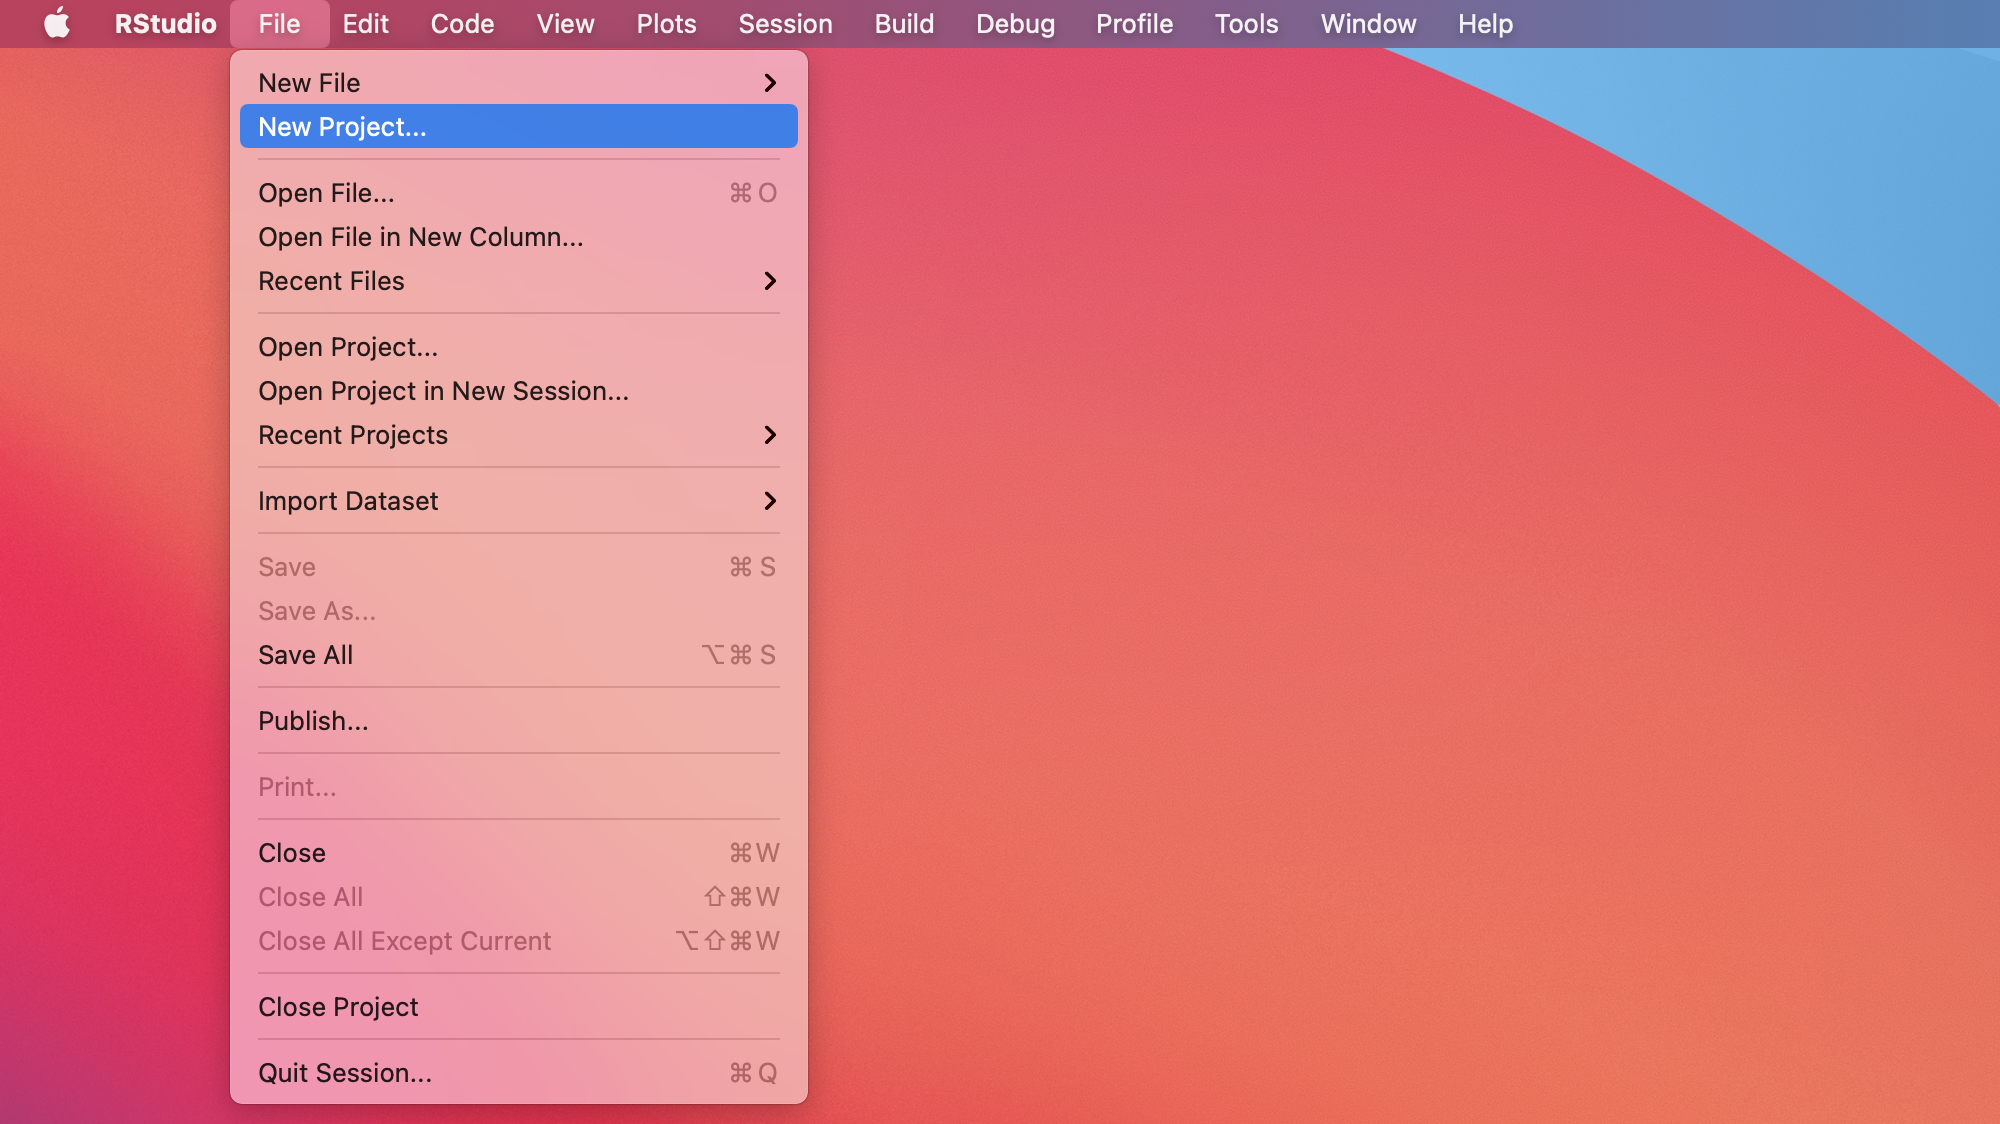
\includegraphics{images/chapter_06_img/00_r_project/00_r_project_file_menu.png}
\item
  Select \texttt{New\ Directory} from the popup window.

  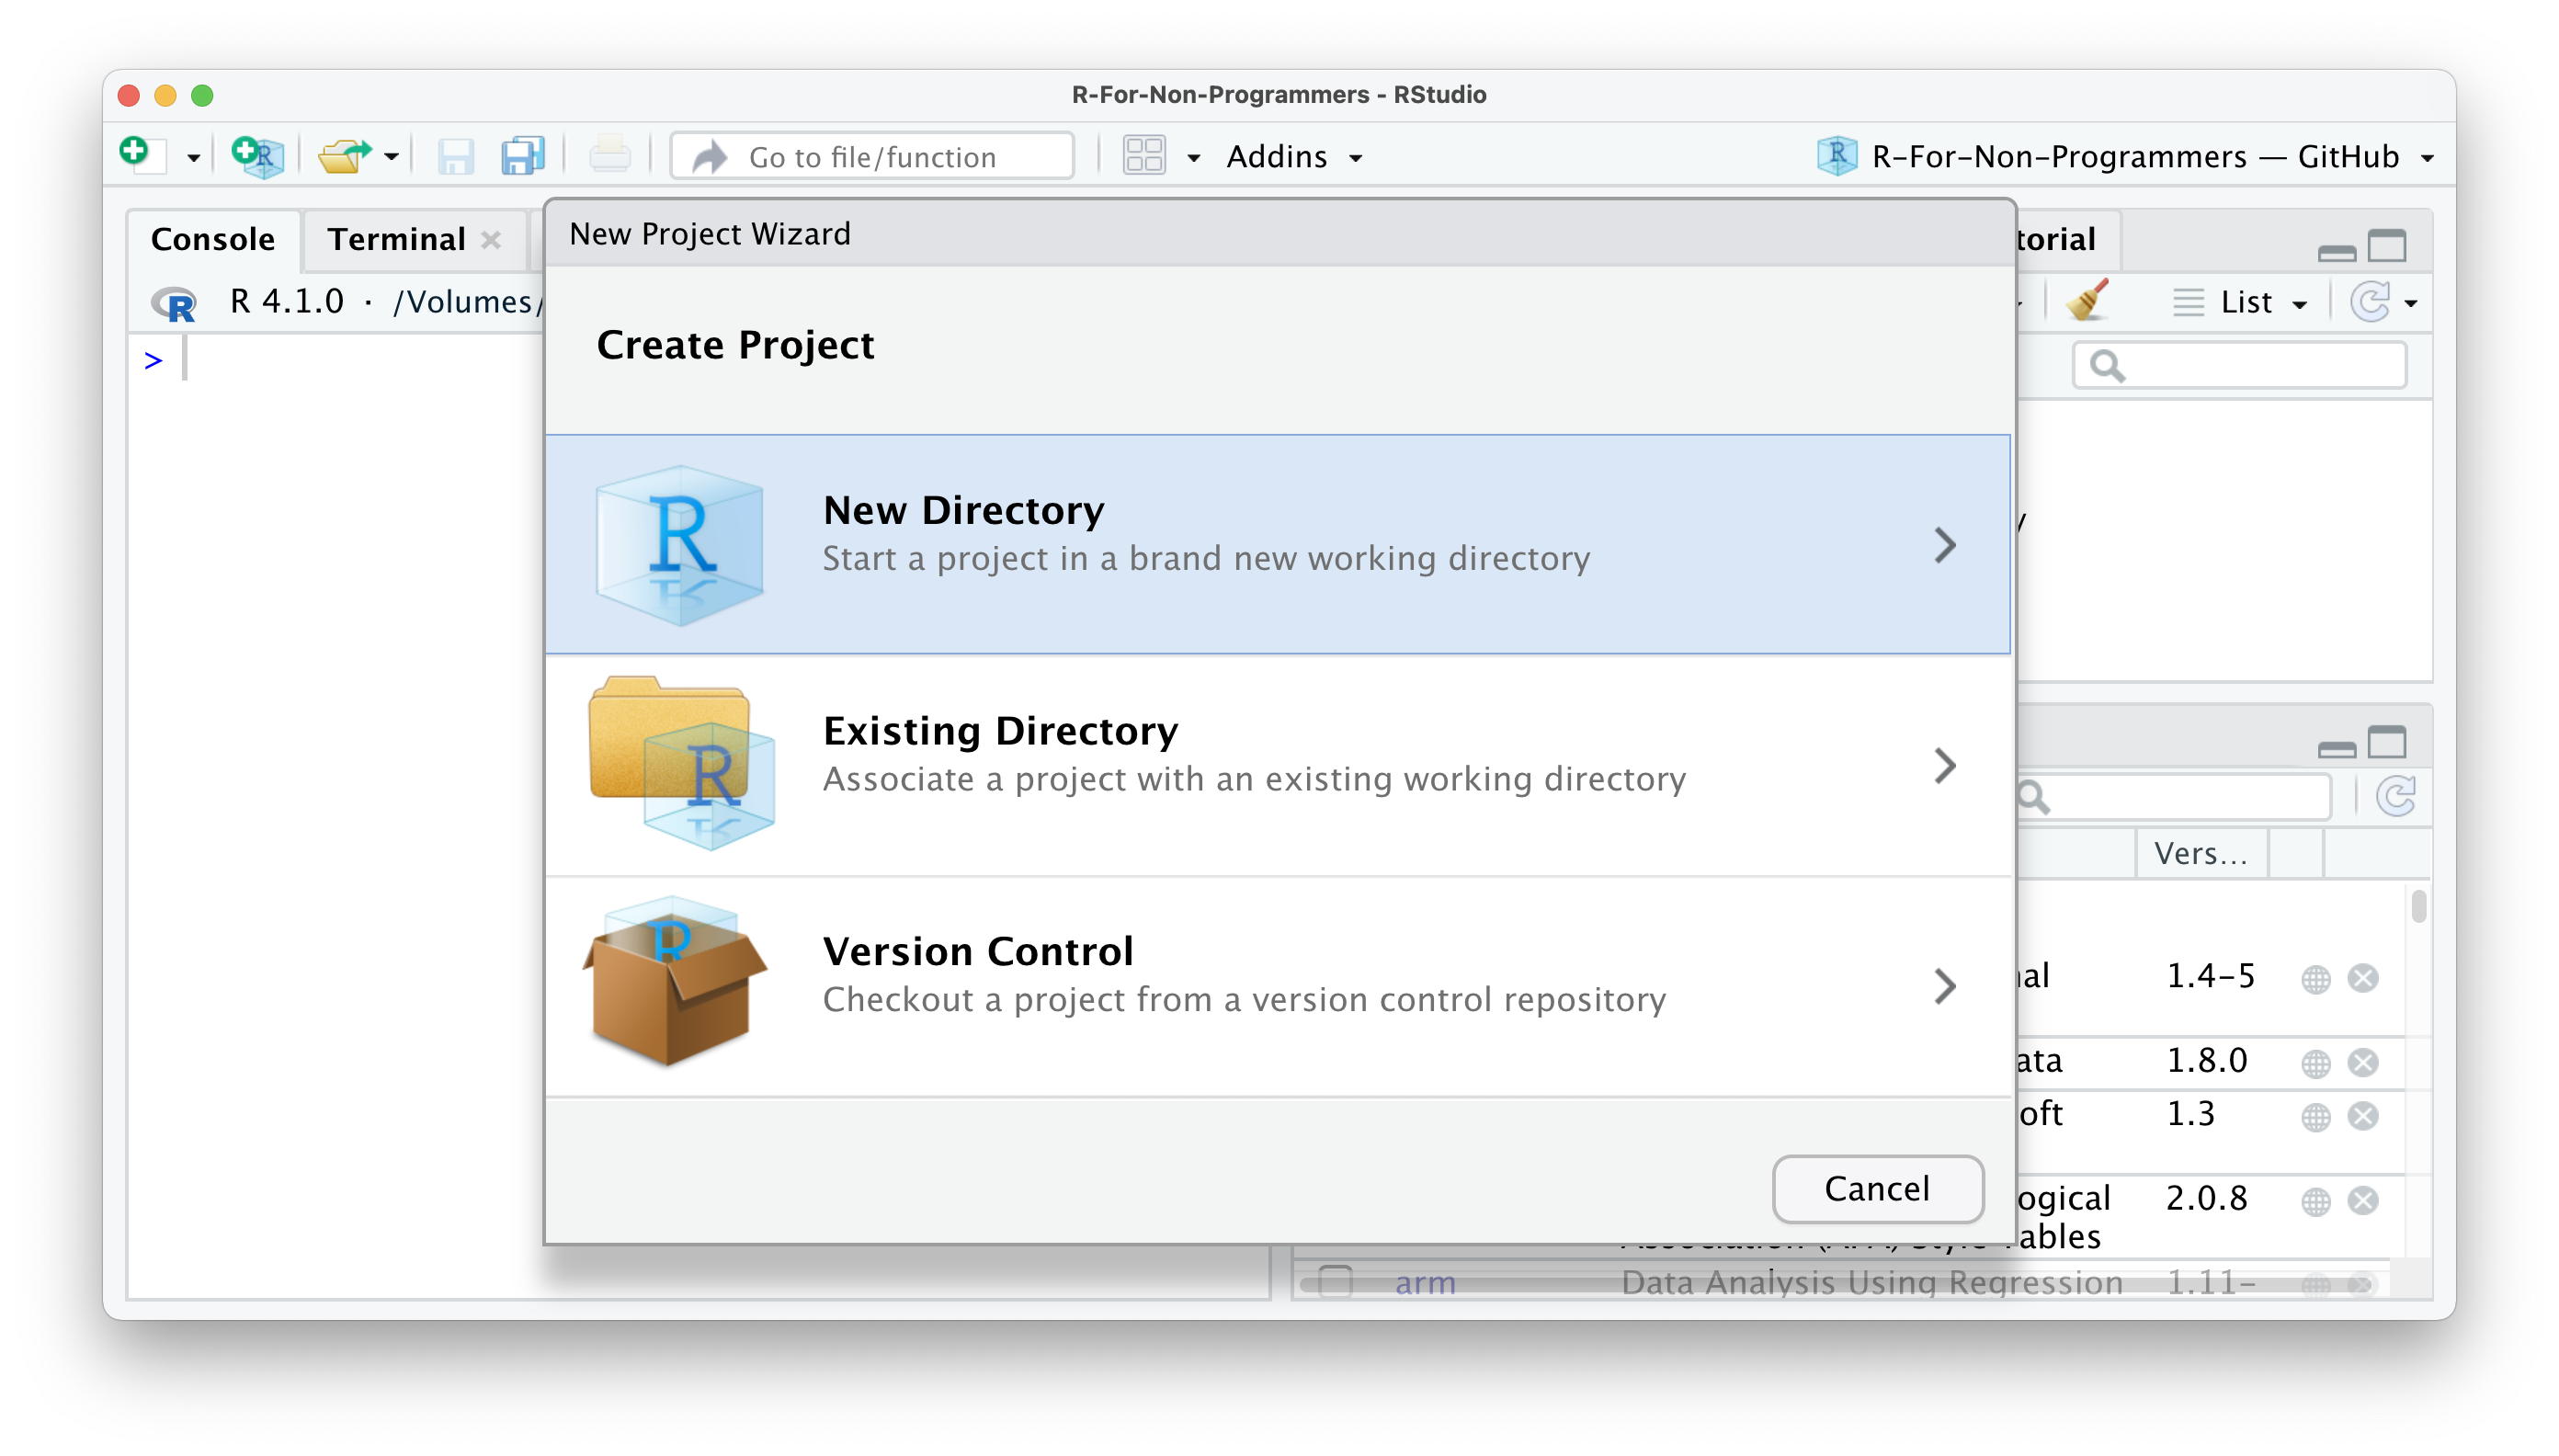
\includegraphics{images/chapter_06_img/00_r_project/01_r_project_new_directory.png}
\item
  Next, select \texttt{New\ Project}.

  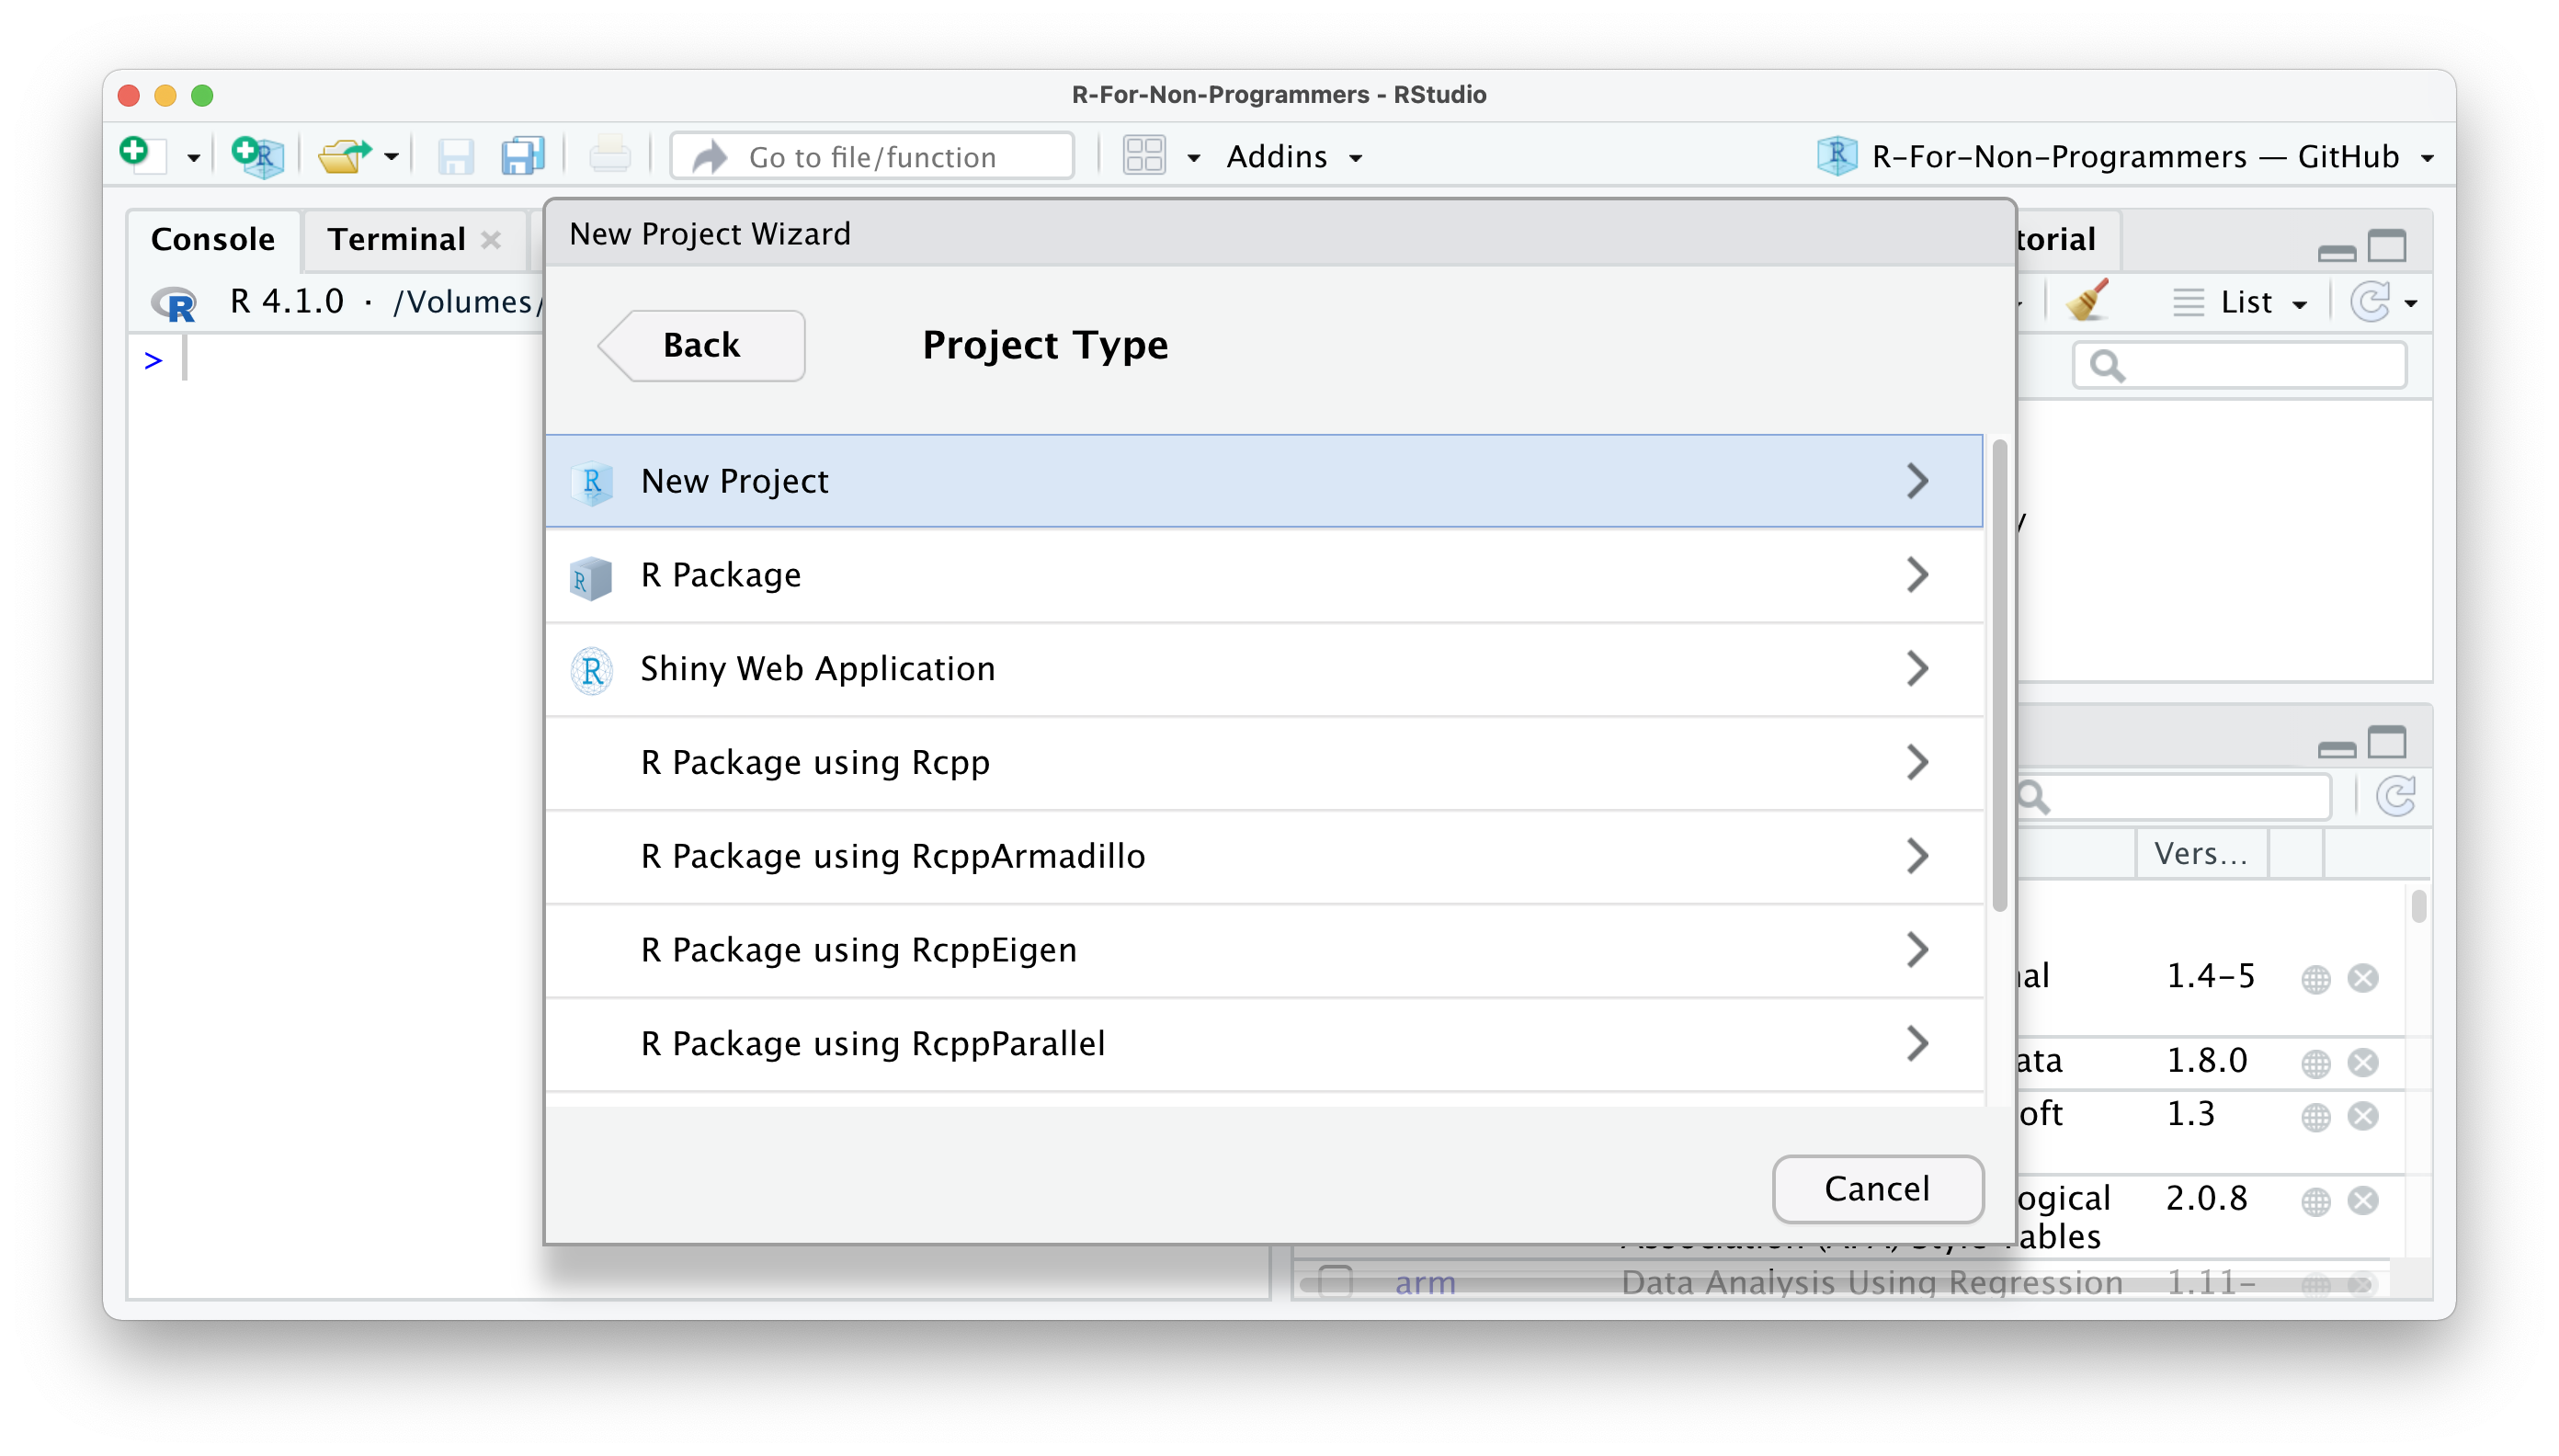
\includegraphics{images/chapter_06_img/00_r_project/02_r_project_new_project.png}
\item
  Pick a meaningful name for your project folder, i.e.~the \texttt{Directory\ Name}. Ensure this project folder is created in the right place. You can change the \texttt{subdirectory} by clicking on \texttt{Browse\ldots{}}. Ideally the subdirectory is a place where you usually store your research projects.

  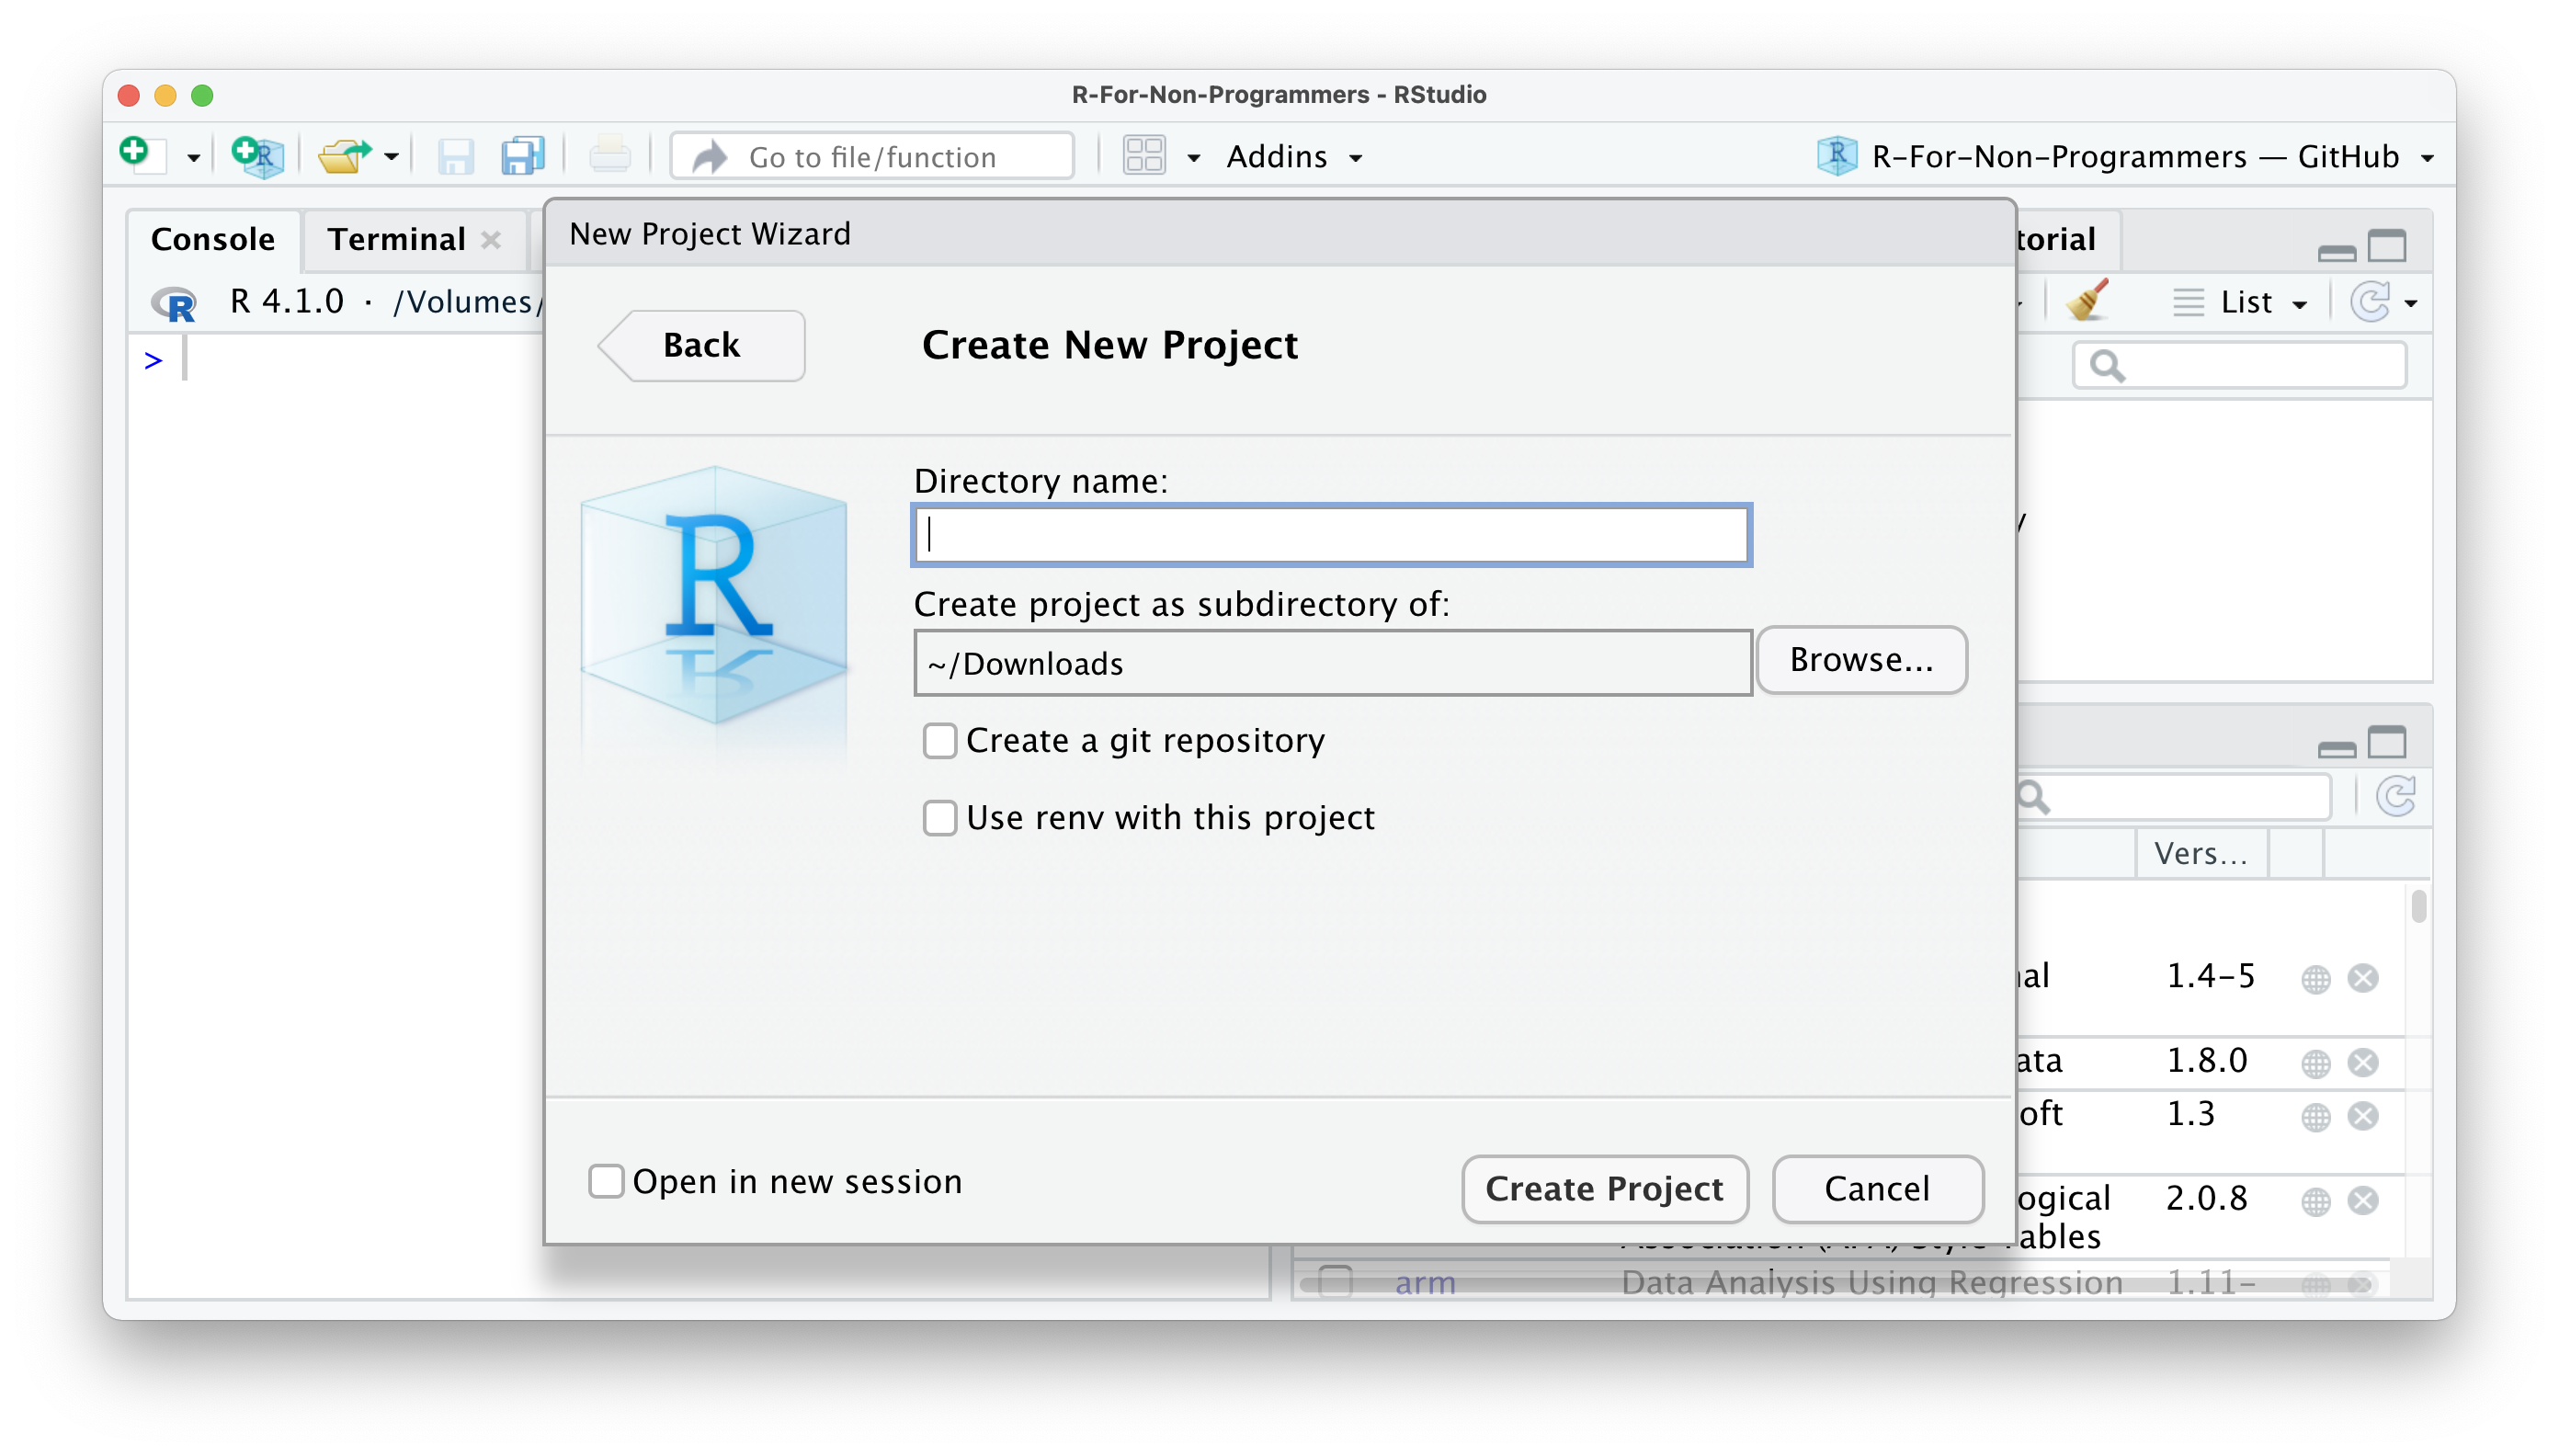
\includegraphics{images/chapter_06_img/00_r_project/03_r_project_specs.png}
\item
  You have the option to \texttt{Create\ a\ git\ repository}. This is only relevant if you already have a GitHub account and wish to use version control. For now, you can happily ignore it.
\item
  Lastly, tick \texttt{Open\ in\ new\ session}. This will open your R Project in a new RStudio window.

  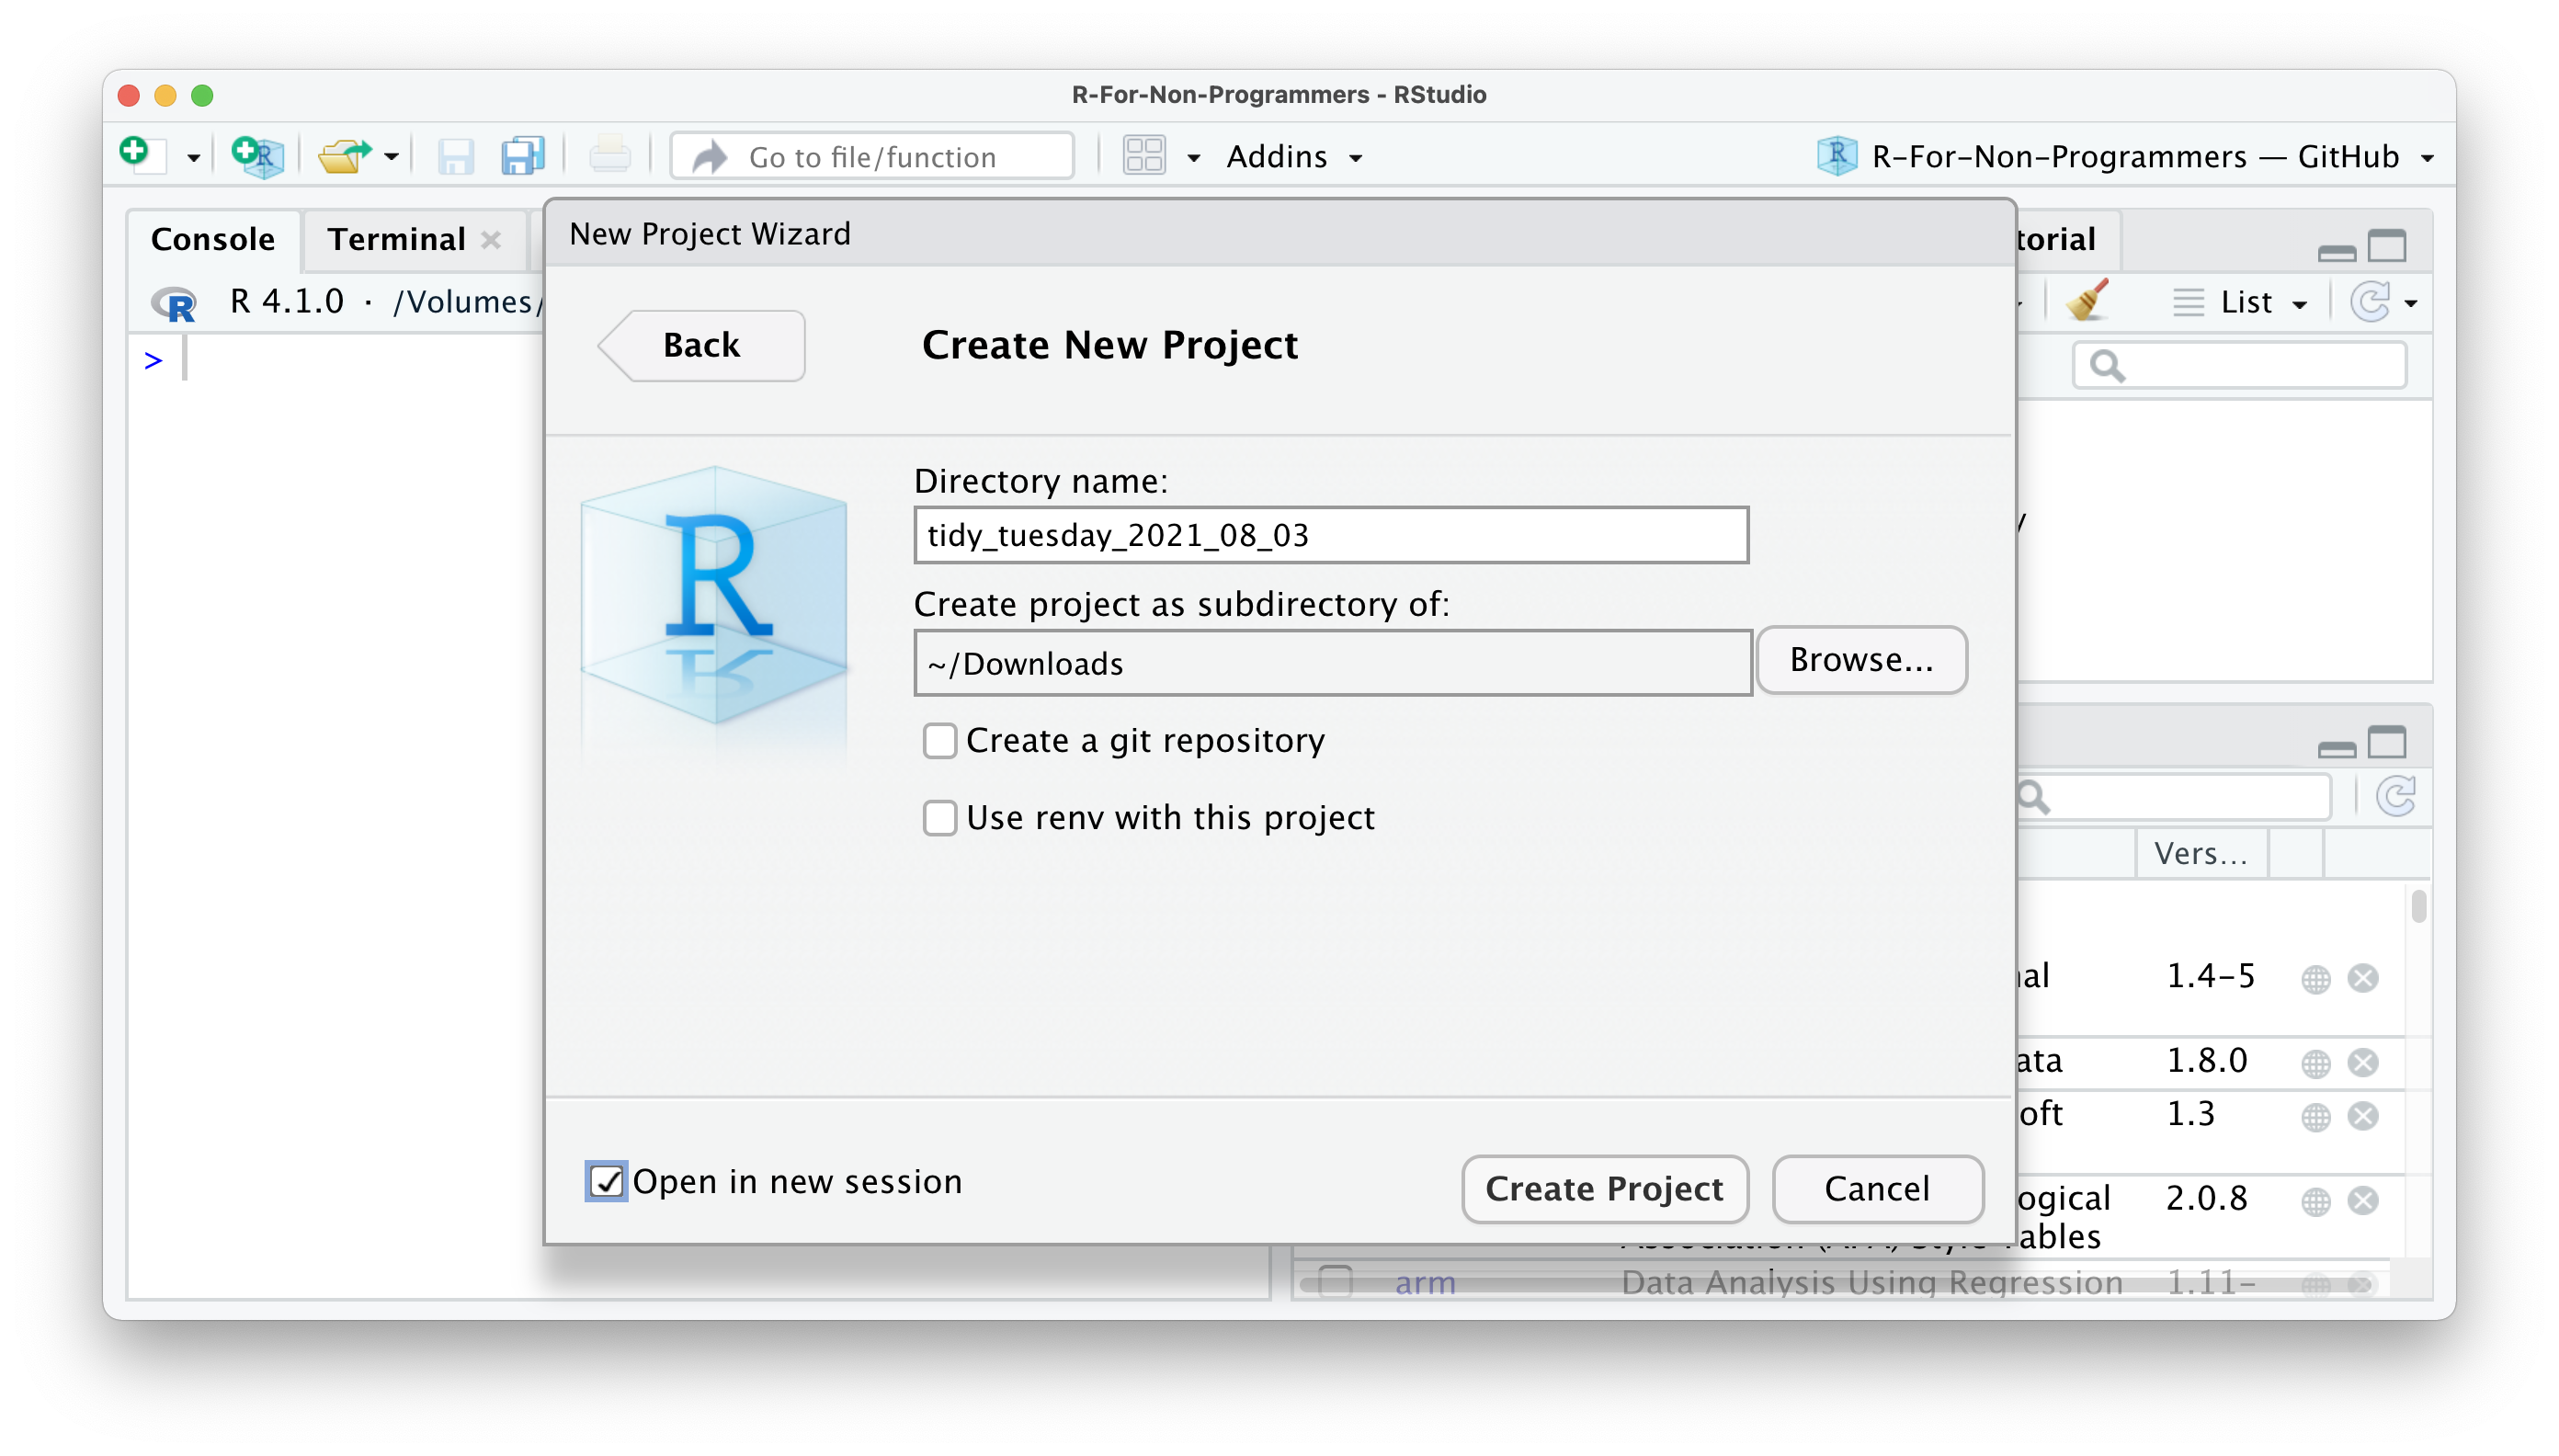
\includegraphics{images/chapter_06_img/00_r_project/04_r_project_directory_name.png}
\item
  Once you are happy with your choices, you can click \texttt{Create\ Project}. This will open a new R Session, and you can start working on your project.

  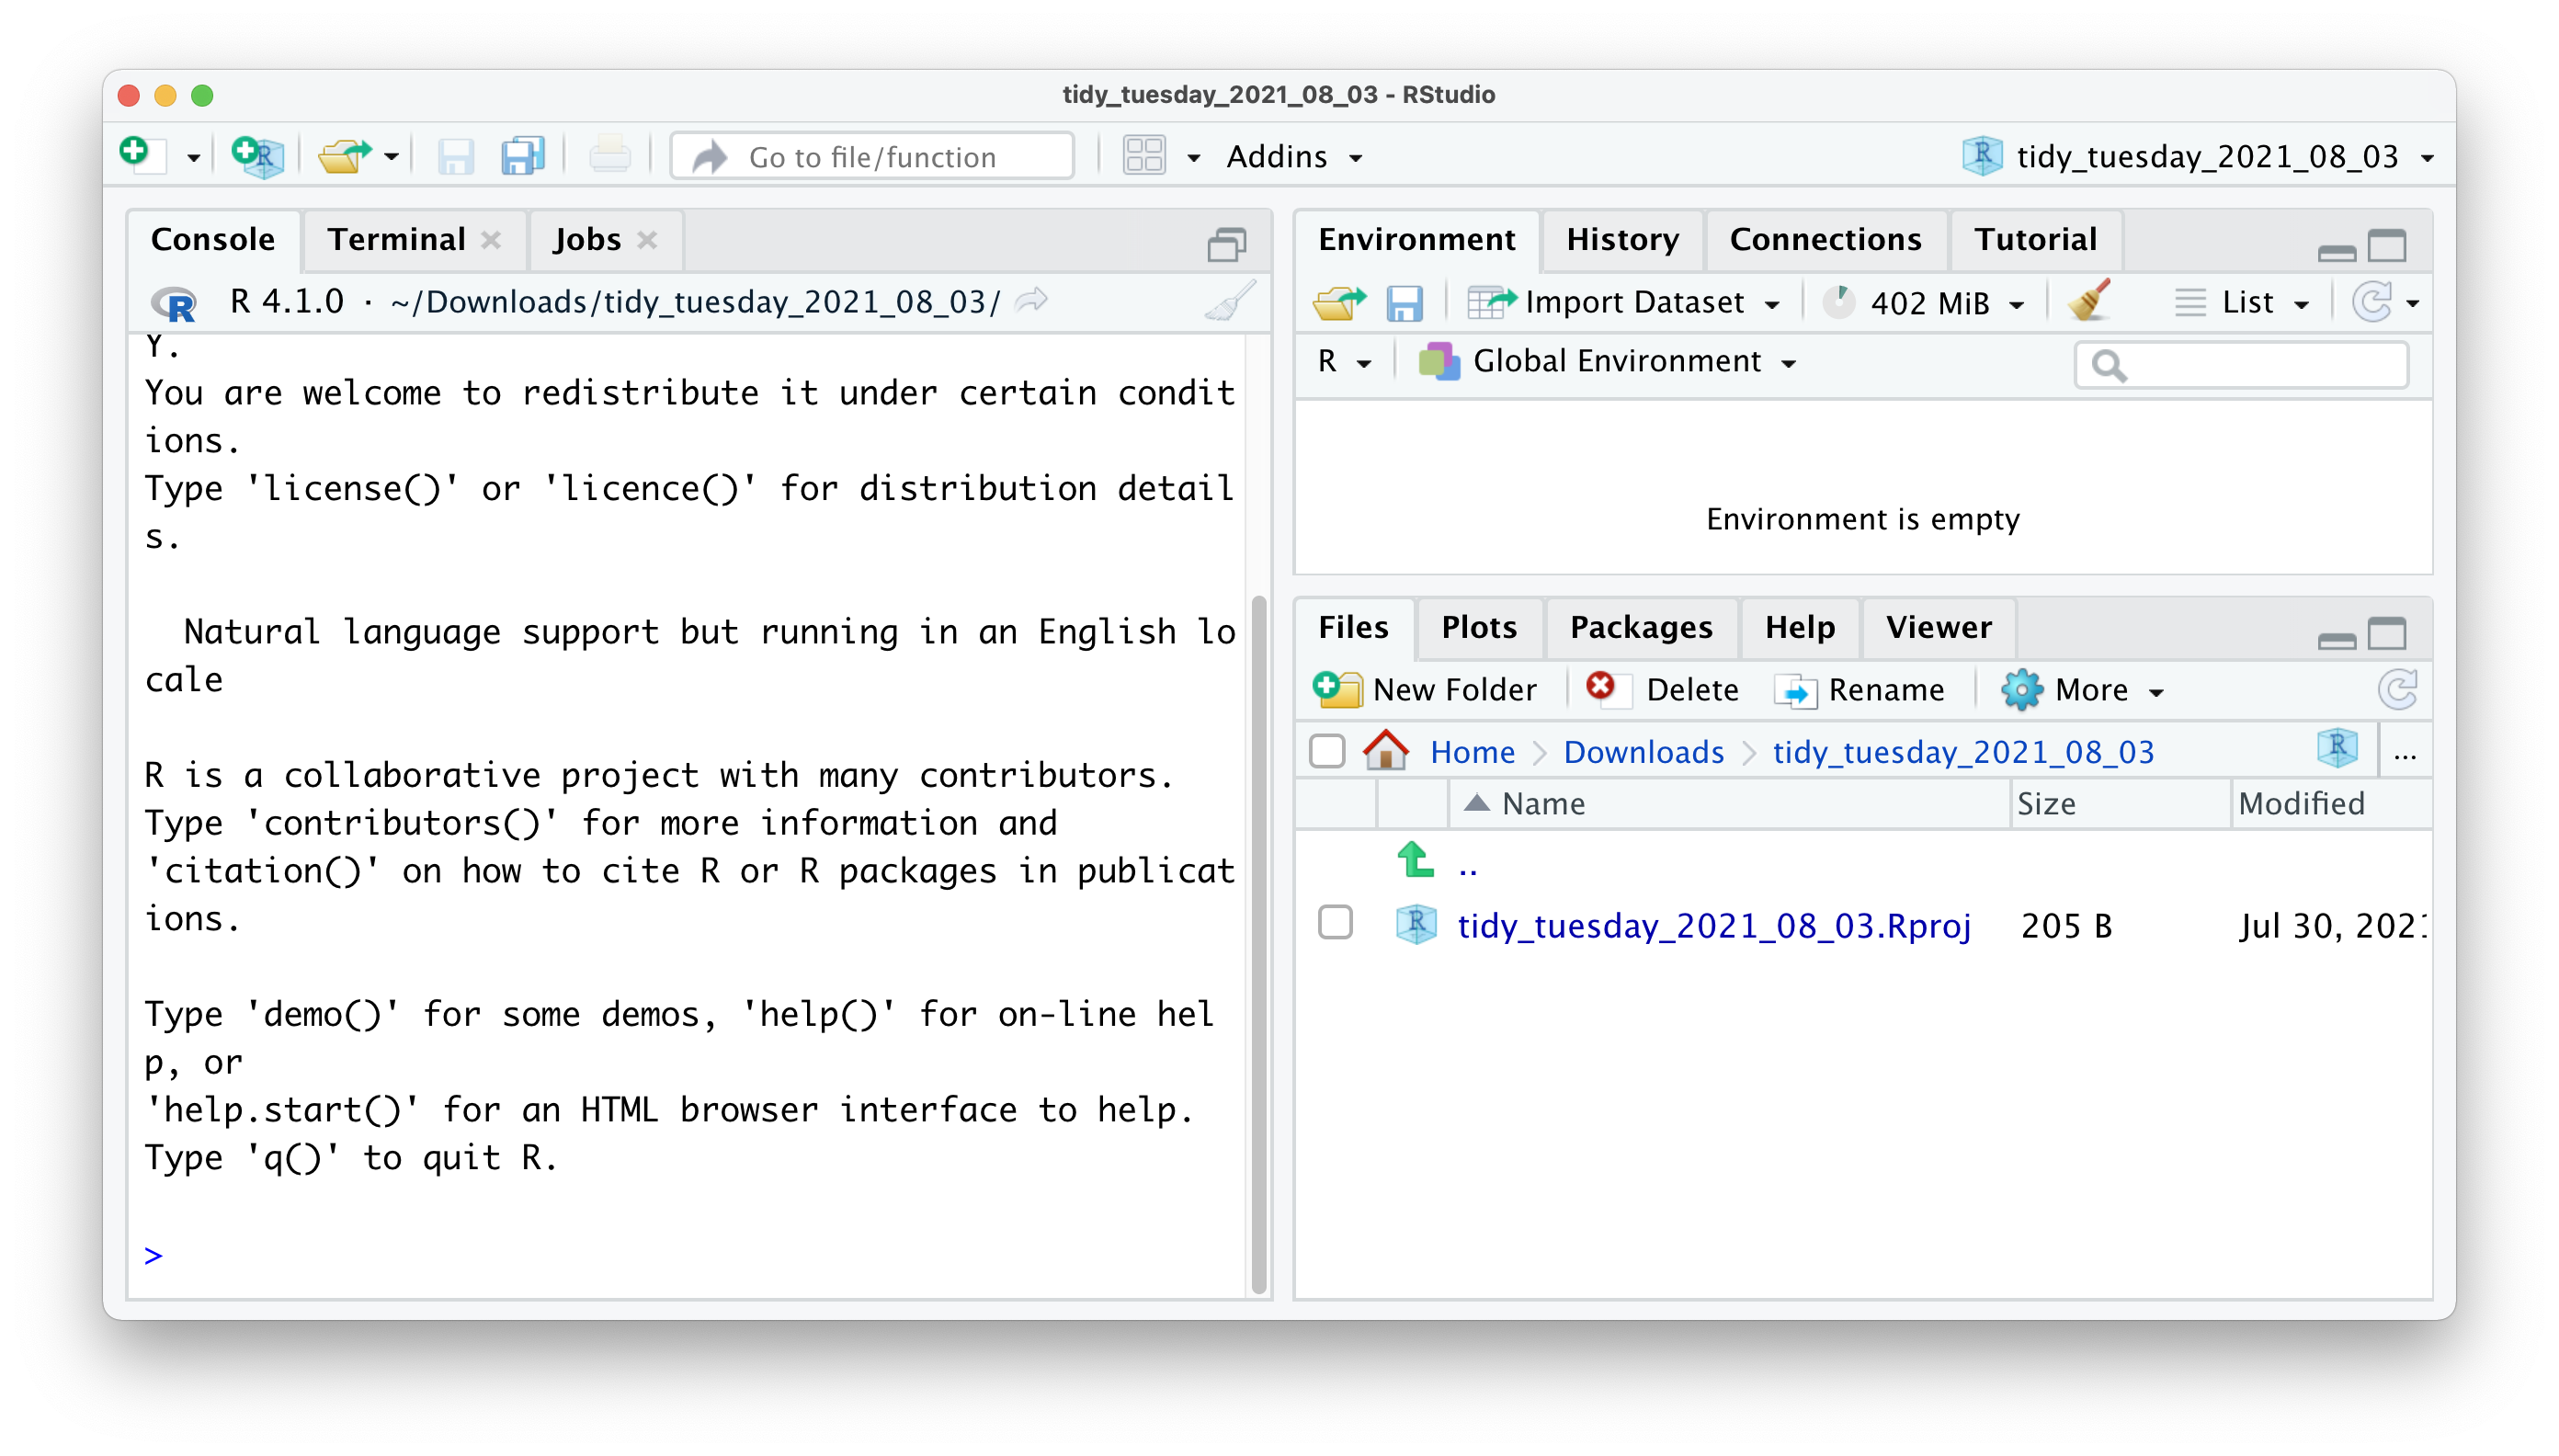
\includegraphics{images/chapter_06_img/00_r_project/05_r_project_new_session.png}
\end{enumerate}

If you look carefully, you can see that your RStudio is now `branded' with your project name. At the top of the window, you see the project name, the files pane shows the root directory where all your files will be, and even the console shows on top the file path of your project. You could set all this up manually, but I would not recommend it, not the least because it is easy to work with R Projects.

\hypertarget{organising-your-projects}{%
\section{Organising your projects}\label{organising-your-projects}}

This section is not directly related to RStudio, R or data analysis in general. Instead, I want to convey to you that a good folder structure can go a long way. It is an excellent habit to start thinking about folder structures before you start working on your project. Placing your files into dedicated folders, rather than keeping them loosely in one container, will speed up your work and save you from the frustration of not finding the files you need. I have a template that I use regularly. You can either create it from scratch in RStudio or open your file browser and create the folders there. RStudio does not mind which way you do it. If you want to spend less time setting this up, you might want to use the function \texttt{create\_dr()} from the \texttt{r4np} package. It creates all the folders as shown in Figure \ref{fig:folder-structure}.

\begin{Shaded}
\begin{Highlighting}[]
\CommentTok{\# Install \textquotesingle{}r4np\textquotesingle{} from GitHub}
\NormalTok{devtools}\SpecialCharTok{::}\FunctionTok{install\_github}\NormalTok{(}\StringTok{"ddauber/r4np"}\NormalTok{)}

\CommentTok{\# Create the template structure}
\NormalTok{r4np}\SpecialCharTok{::}\FunctionTok{create\_dr}\NormalTok{()}
\end{Highlighting}
\end{Shaded}

To create a folder, click on \texttt{New\ Folder} in the Files pane. I usually have at least the following folders for every project I am involved in:

\begin{itemize}
\item
  A folder for my raw data. I store `untouched' datasets in it. With `untouched', I mean they have not been processed in any way and are usually files I downloaded from my data collection tool, e.g.~online questionnaire platform.
\item
  A folder with `tidy' data. This is usually data I exported from R after cleaning it, i.e.~after data wrangling (see Chapter \ref{data-wrangling}).
\item
  A folder for my R scripts
\item
  A folder for my plots
\item
  A folder for reports
\end{itemize}

Thus, in RStudio, it would look something like this:

\begin{figure}

{\centering 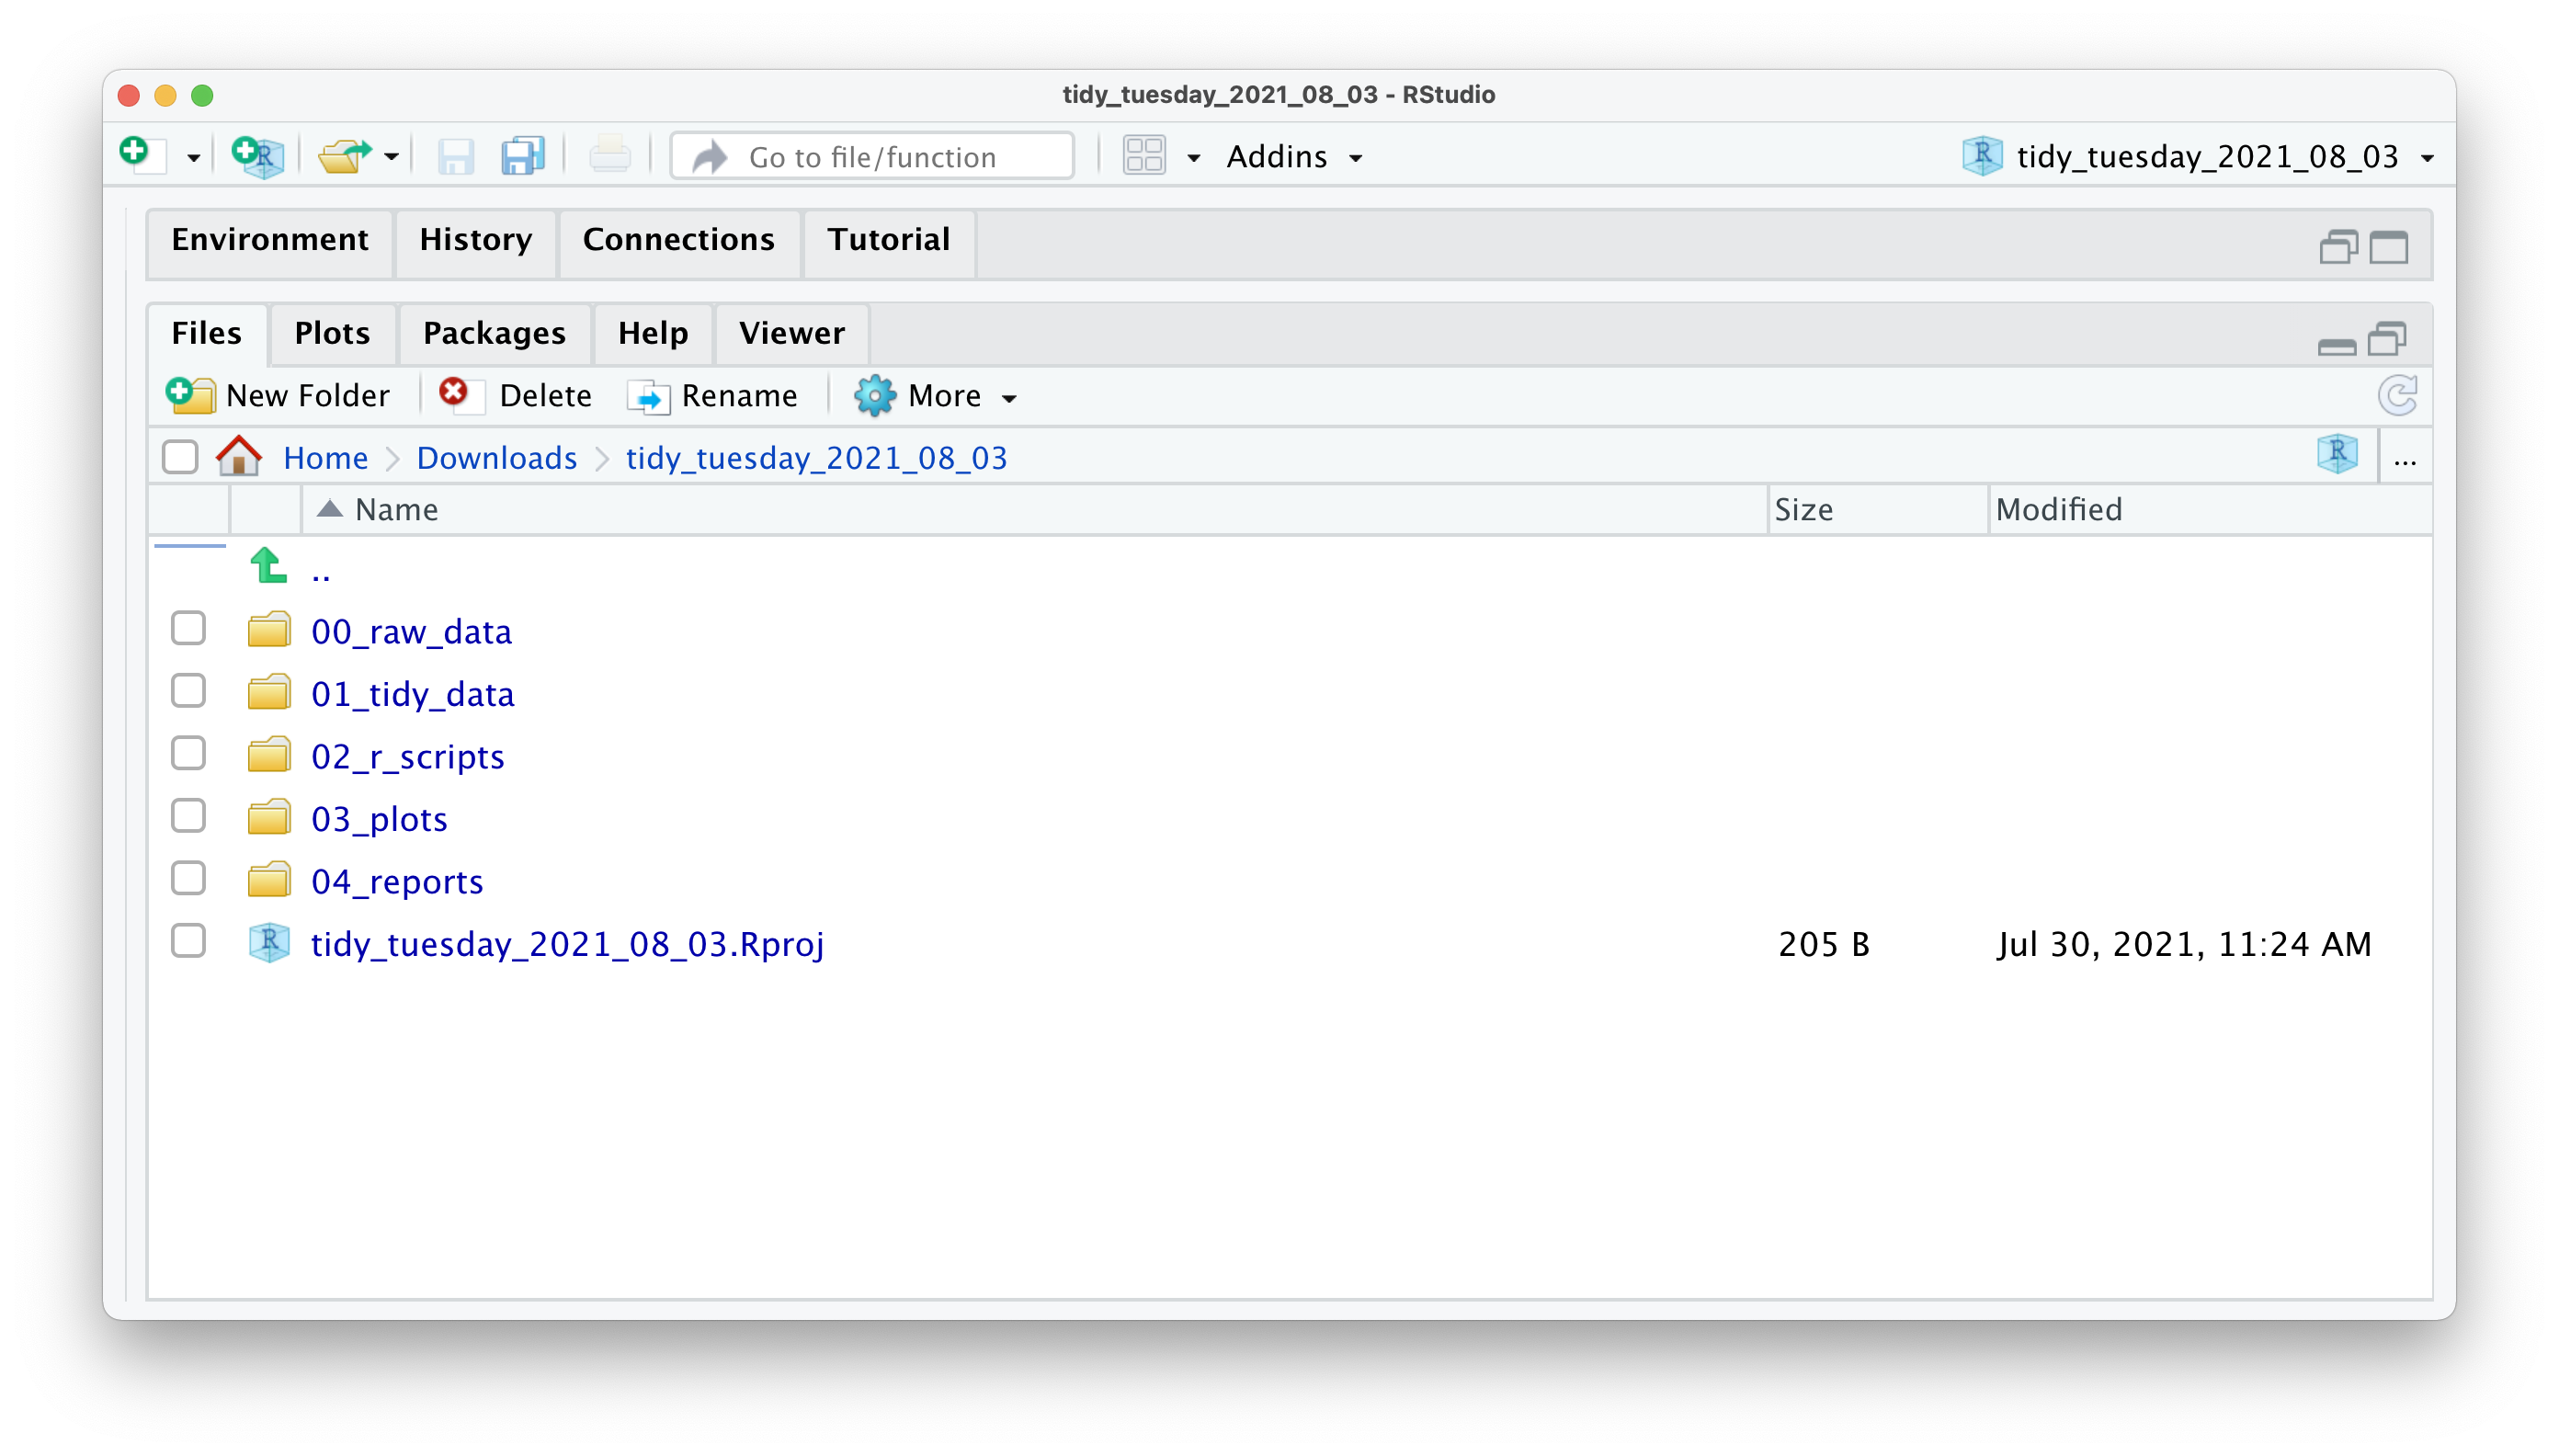
\includegraphics[width=38.67in]{images/chapter_06_img/01_organising_work/00_organising_work} 

}

\caption{An example of a scalable folder structure for your project}\label{fig:folder-structure}
\end{figure}

You probably noticed that my folders have numbers in front of them. I do this to ensure that all folders are in the order I want them to be, usually not the alphabetical order my computer suggests. I use two digits because I may have more than nine folders for a project, and folder ten would otherwise be listed as the third folder in this list. With this filing strategy in place, it will be easy to find whatever I need. Even others can easily understand what I stored where. It is simply `tidy', similar to how we want our data to be.

\hypertarget{creating-an-r-script}{%
\section{Creating an R Script}\label{creating-an-r-script}}

Code quickly becomes long and complex. Thus, it is not very convenient to write it in the console. So, instead, we can write code into an R Script. An R Script is a document that RStudio recognises as R programming code. Files that are not R Scripts, like \texttt{.txt}, \texttt{.rtf} or \texttt{.md}, can also be opened in RStudio, but any code written in it will not be automatically recognised.

When opening an R script or creating a new one, it will display in the source window (see Chapter \ref{the-source-window}). Some refer to this window as the `script editor'. An R Script starts as an empty file. Good coding etiquette (see Chapter \ref{coding-etiquette} demands that we use the first line to indicate what this file does by using a comment \texttt{\#}. Here is an example for our `TidyTuesday' R Project.

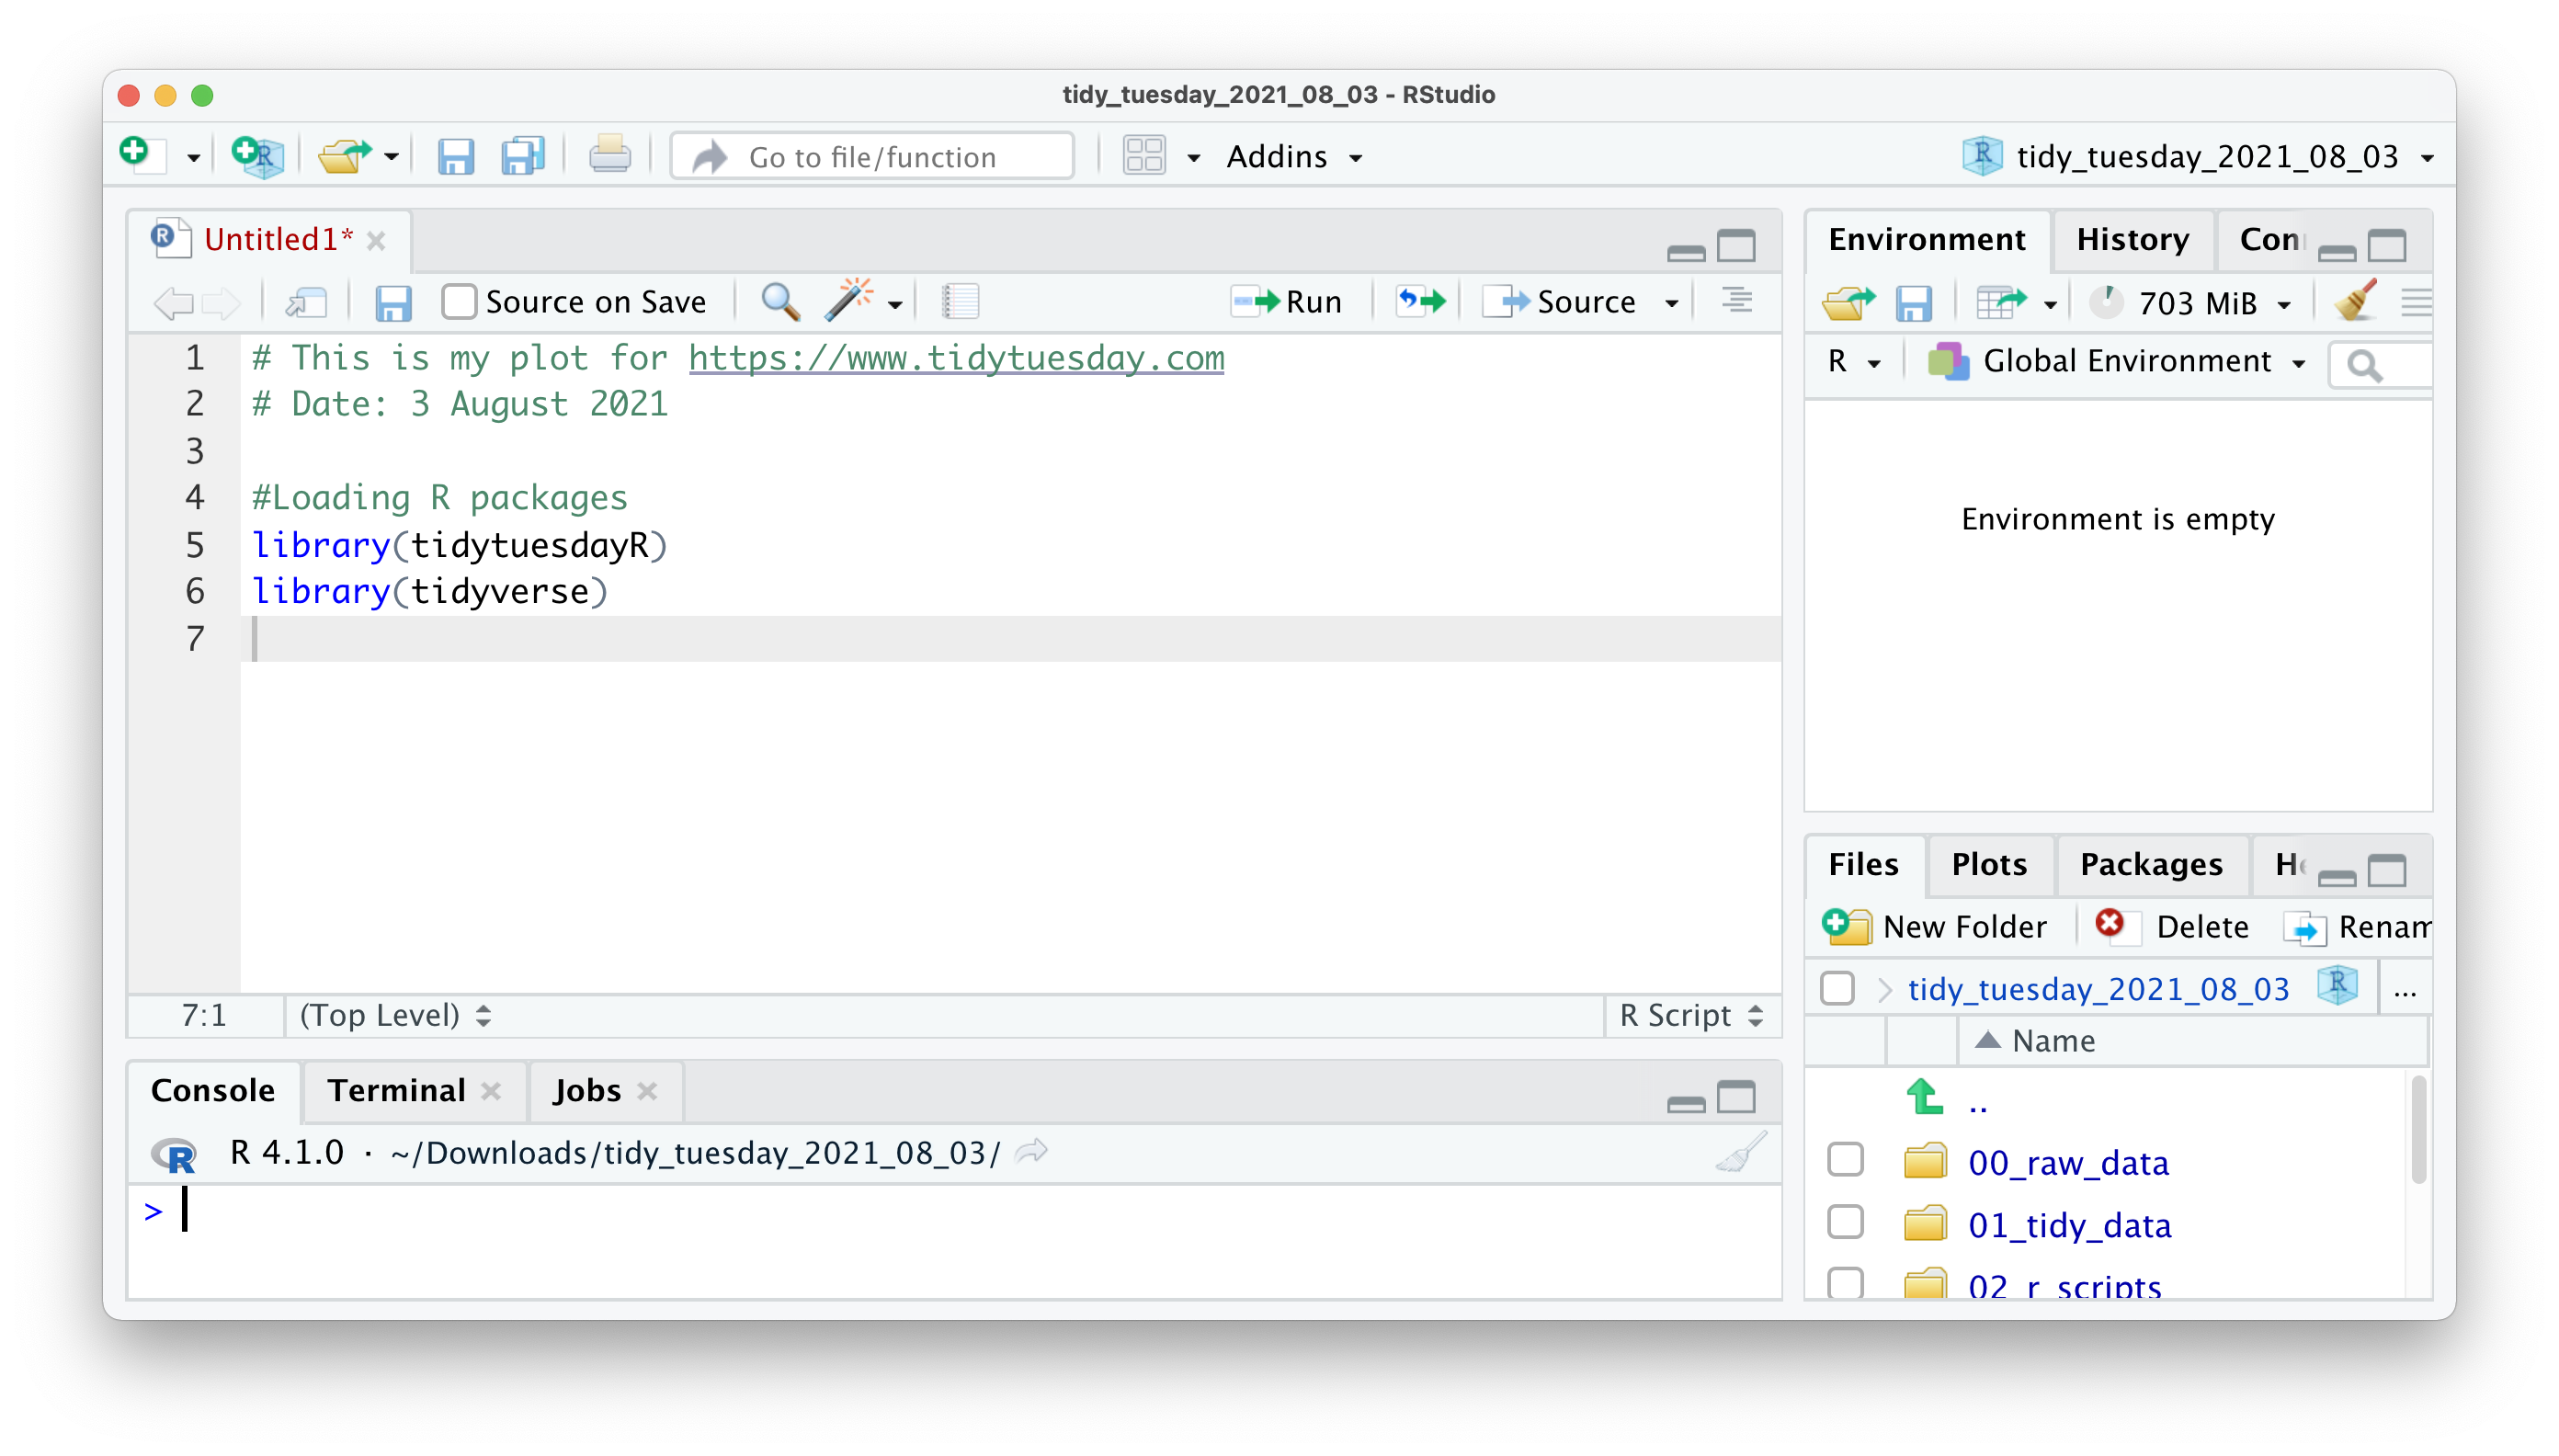
\includegraphics{images/chapter_06_img/02_r_script/00_r_script.png}

All examples in this book can easily be copied and pasted into your own R Script. However, for some code you will have to install the R package \texttt{r4np} (see \protect\hyperlink{install_r4np}{above}). Let's try it with the following code. The plot this code creates reveals which car manufacturer produces the most efficient cars.

\begin{Shaded}
\begin{Highlighting}[]
\FunctionTok{library}\NormalTok{(tidyverse)}

\NormalTok{mpg }\SpecialCharTok{\%\textgreater{}\%} \FunctionTok{ggplot}\NormalTok{(}\FunctionTok{aes}\NormalTok{(}\AttributeTok{x =} \FunctionTok{reorder}\NormalTok{(manufacturer, }\FunctionTok{desc}\NormalTok{(hwy), }\AttributeTok{FUN =}\NormalTok{ median),}
                   \AttributeTok{y =}\NormalTok{ hwy,}
                   \AttributeTok{fill =}\NormalTok{ manufacturer)) }\SpecialCharTok{+}
  \FunctionTok{geom\_boxplot}\NormalTok{() }\SpecialCharTok{+}
  \FunctionTok{coord\_flip}\NormalTok{() }\SpecialCharTok{+}
  \FunctionTok{theme\_minimal}\NormalTok{() }\SpecialCharTok{+}
  \FunctionTok{xlab}\NormalTok{(}\StringTok{"Manufacturer"}\NormalTok{) }\SpecialCharTok{+}
  \FunctionTok{ylab}\NormalTok{(}\StringTok{"Highway miles per gallon"}\NormalTok{)}
\end{Highlighting}
\end{Shaded}

\begin{center}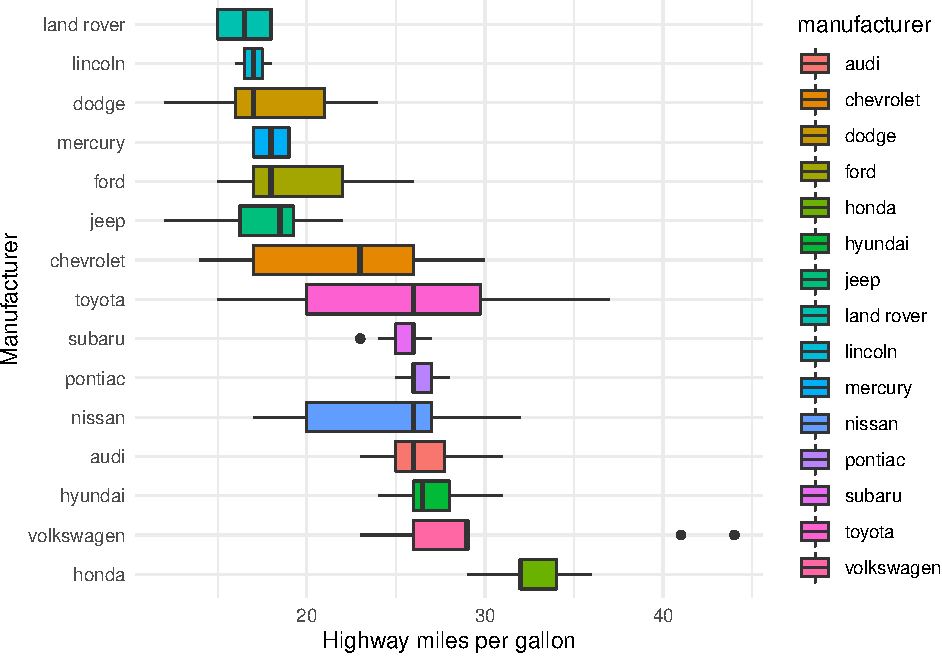
\includegraphics{r_for_non_programmers_files/figure-latex/R Script copy and paste examples-1} \end{center}

You are probably wondering where your plot has gone. Copying the code will not automatically run it in your R Script. However, this is necessary to create the plot. If you tried pressing \texttt{Return\ ↵}, you would only add a new line. Instead, you need to select the code you want to run and press \texttt{Ctrl+Return\ ↵} (PC) or \texttt{Cmd+Return\ ↵} (Mac). You can also use the \texttt{Run} command at the top of your source window, but it is much more efficient to press the keyboard shortcut. Besides, you will remember this shortcut quickly, because we need to use it very frequently. If all worked out, you should see the following:

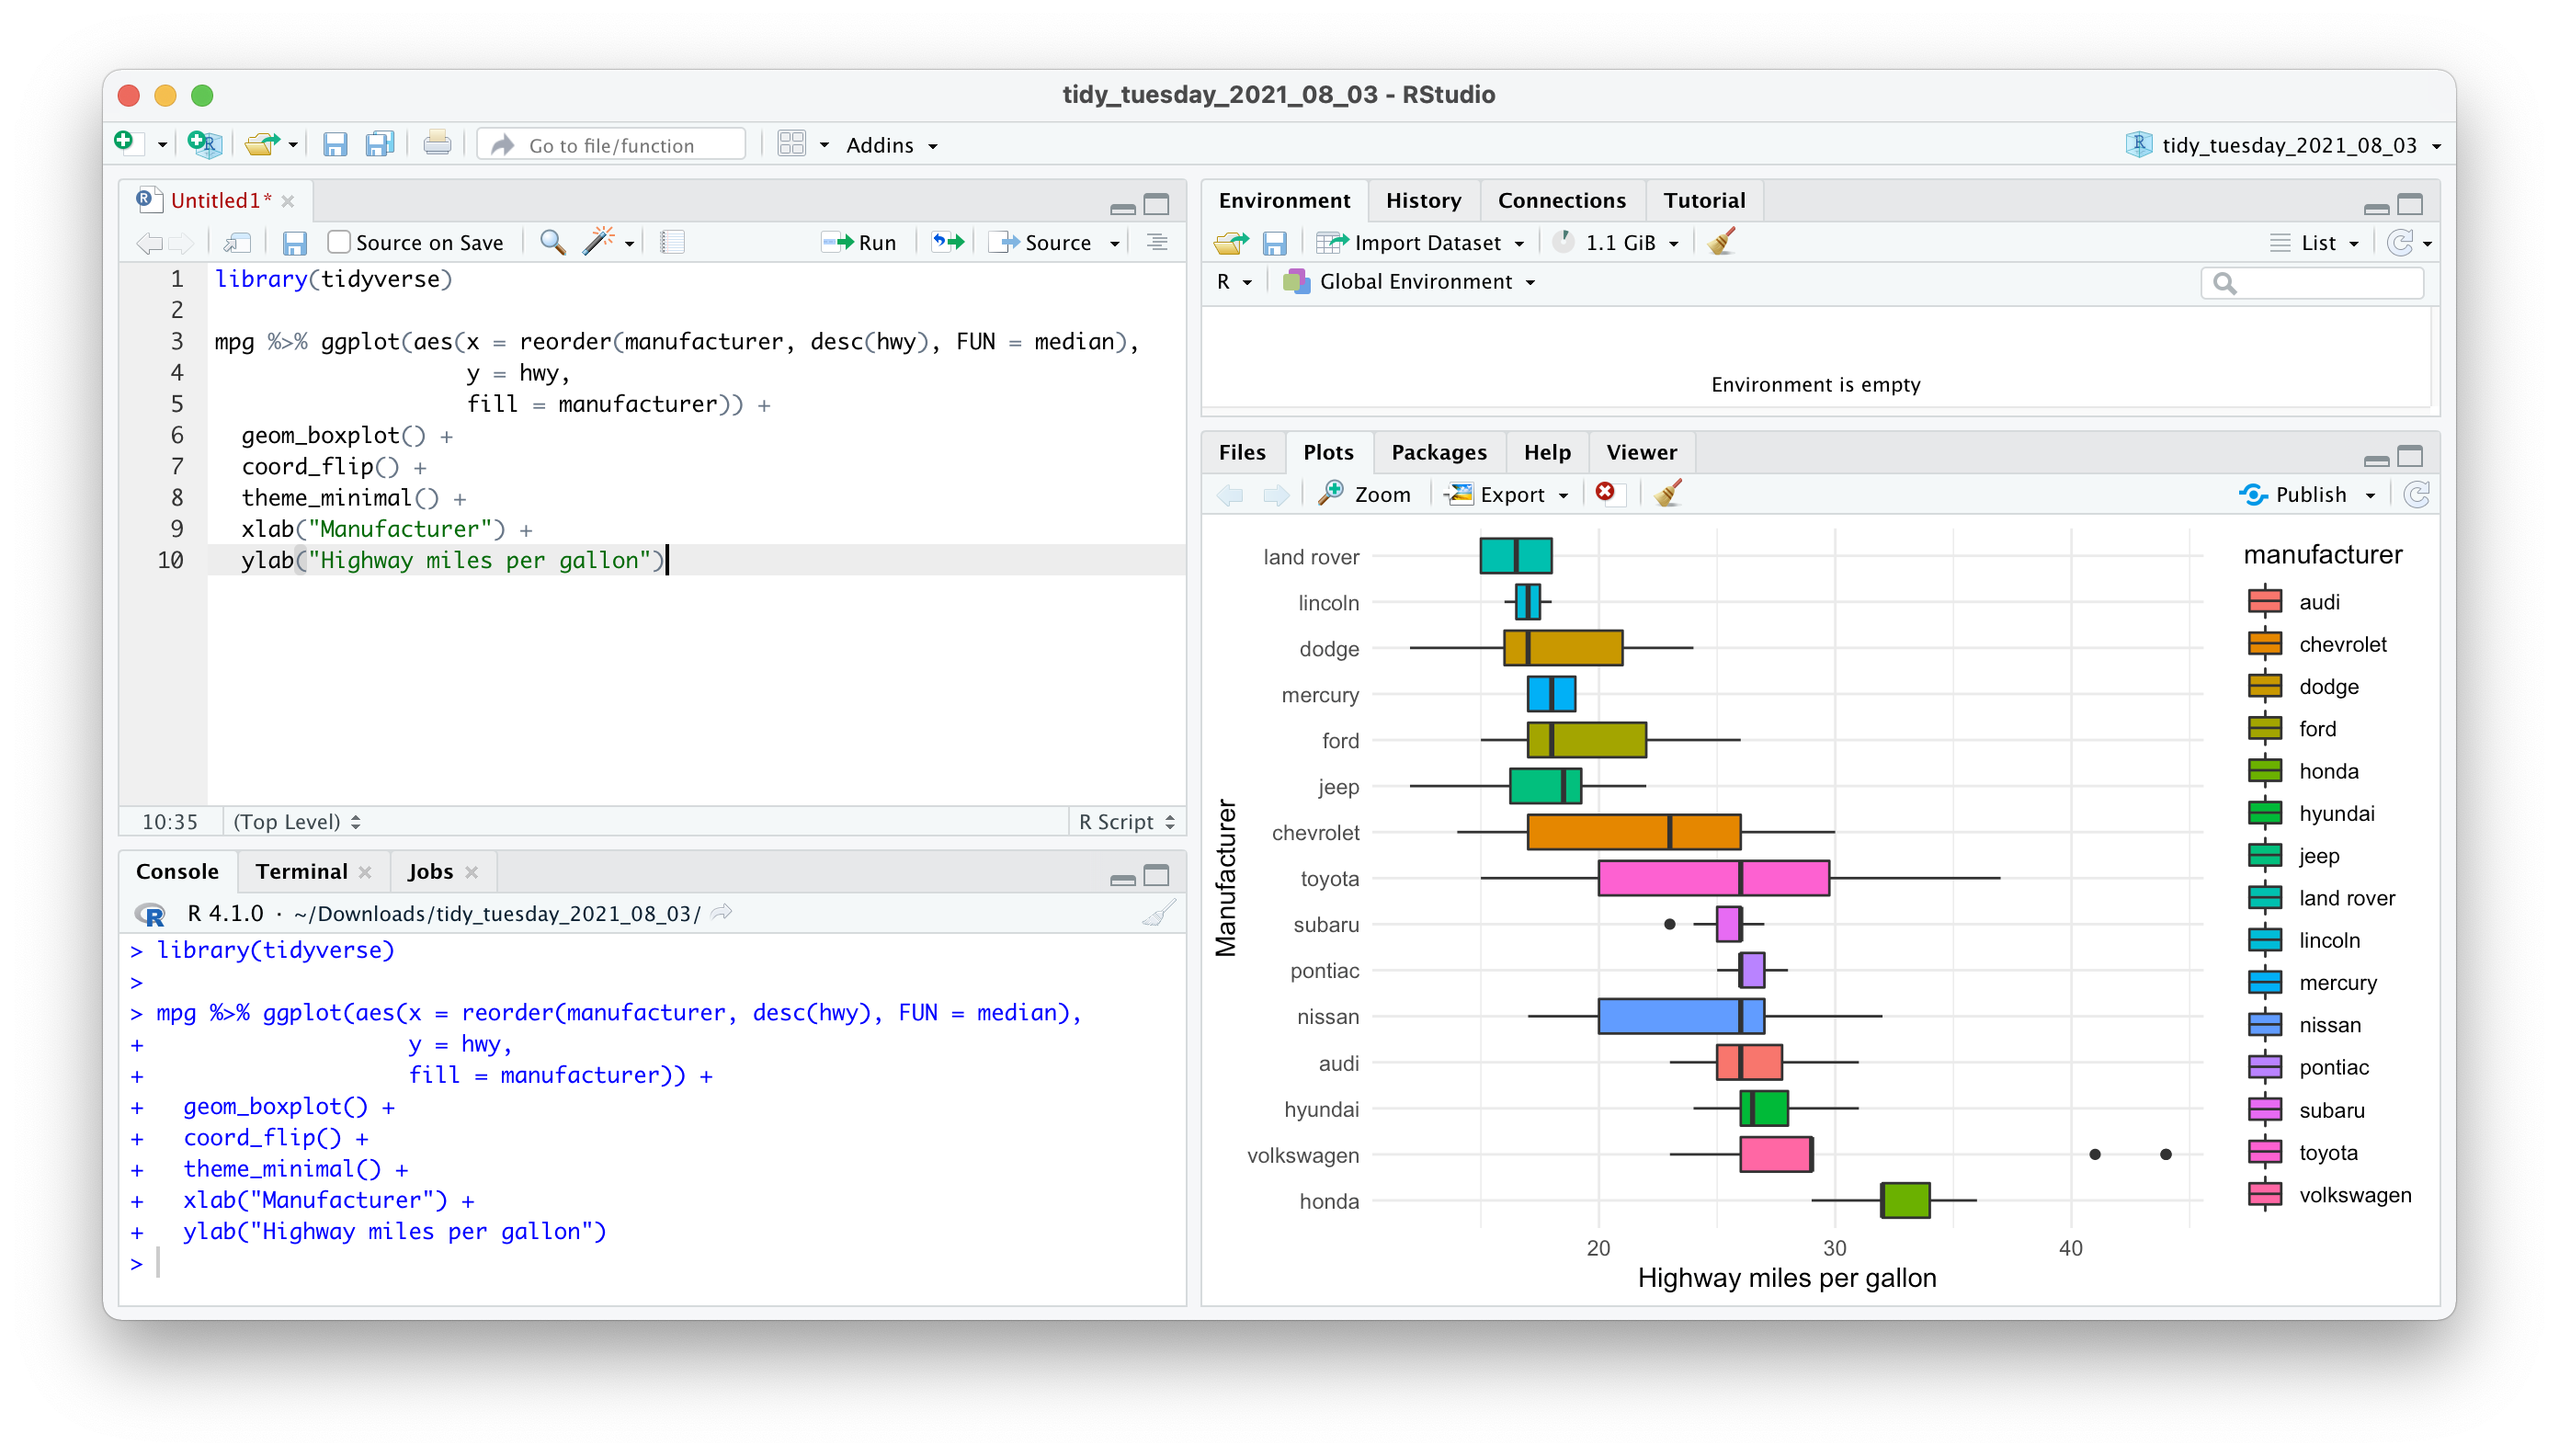
\includegraphics{images/chapter_06_img/02_r_script/01_r_script_example_plot.png}

As you can see, cars from Honda appear to drive furthest with the same amount of fuel (a gallon) compared to other vehicles. Thus, if you are looking for a very economical car, you now know where to find them.

The R Script editor has some conveniences for writing your code that are worth pointing out. You probably noticed that some of the code we have pasted is blue, and some other code is in green. These colours help to make your code more readable because they carry a specific meaning. In the default settings, green stands for any values in \texttt{""}, which usually stands for \texttt{character}s. This is also called `syntax highlighting'.

Moreover, code in R Scripts will be automatically indented to facilitate reading. If for whatever reason, the indentation does not happen, or you accidentally undo it, you can reindent a line with \texttt{Ctrl+I} (PC) or \texttt{Cmd+I} (Mac).

Lastly, the console and the R Script editor both feature code completion. This means that when you start typing a the name of function, R will provide suggestions. These are extremely helpful and make programming a lot faster. Once you found the function you were looking for, you press \texttt{Return\ ↵} to insert it. Here is an example of what happens when you have the package \texttt{tidyverse} loaded and type \texttt{ggpl}. Only functions that are loaded via packages or any object in your environment pane benefit from code completion.

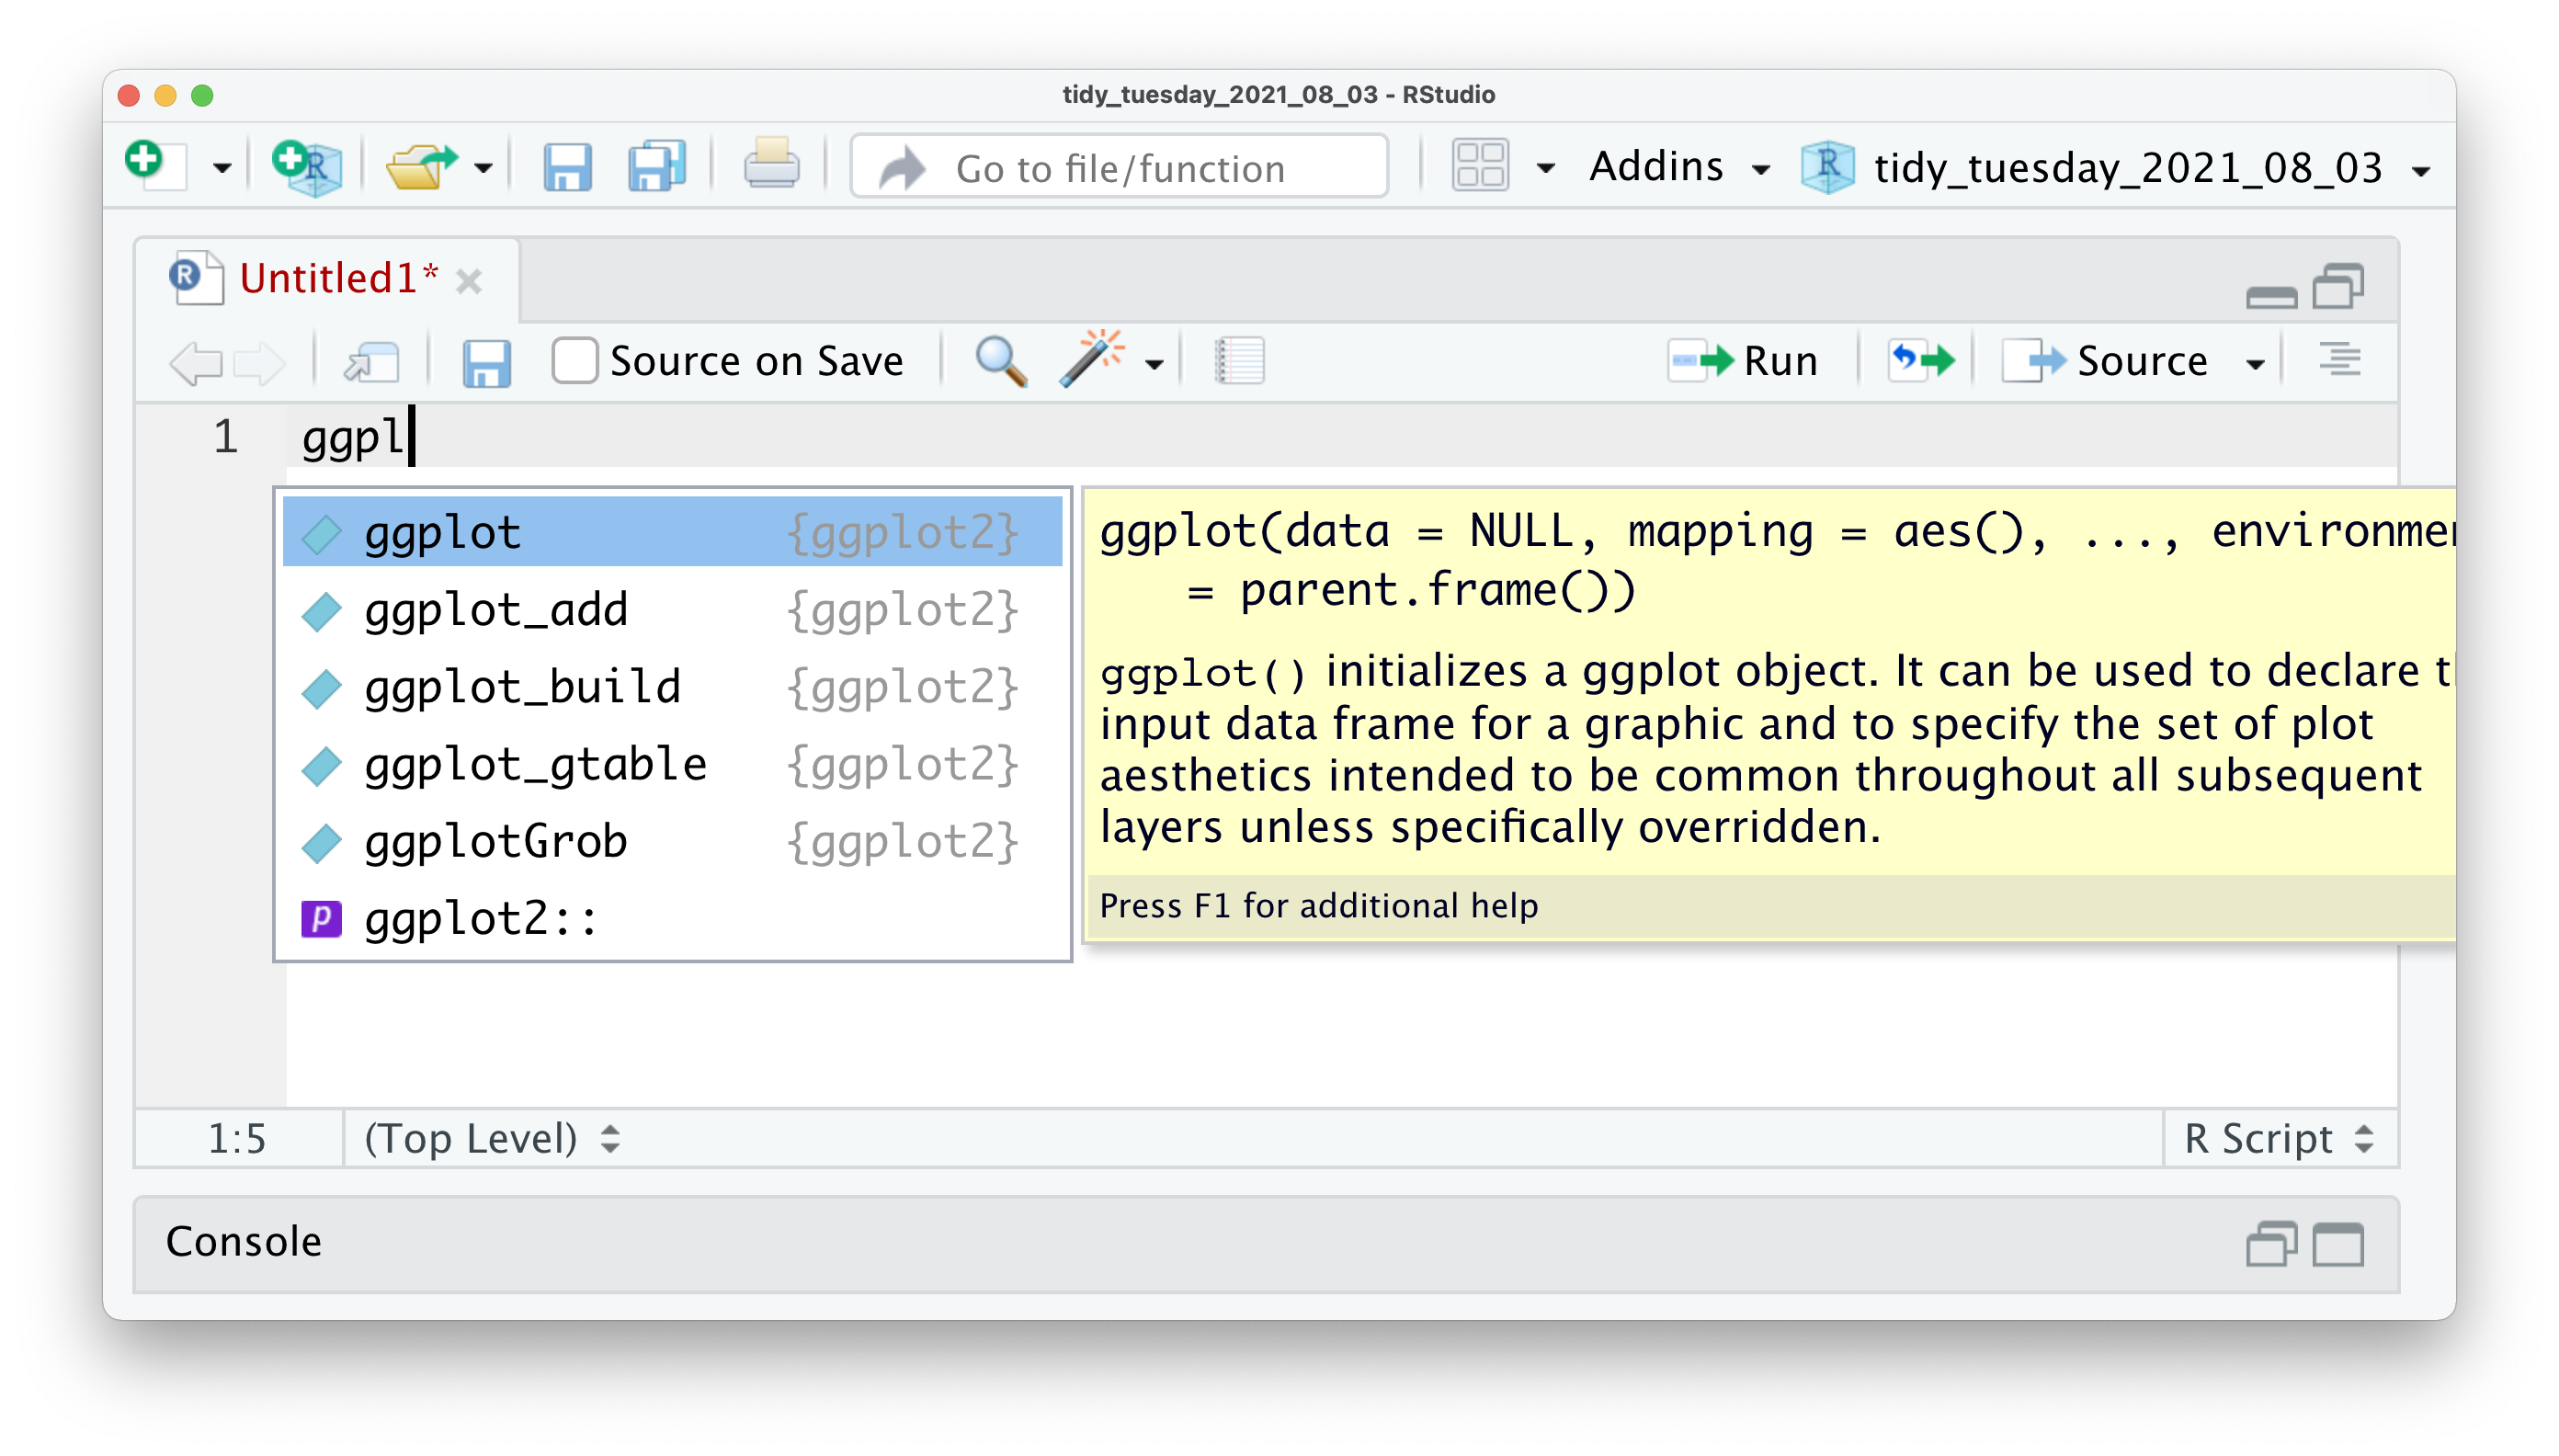
\includegraphics{images/chapter_06_img/02_r_script/02_r script_code_completion.png}

Not only does RStudio show you all the available options, but it also tells you which package this function is from. In this case, all listed functions are from the \texttt{ggplot2} package. Furthermore, when you select one of the options but have not pressed \texttt{Return\ ↵} yet, you also get to see a yellow box, which provides you with a quick reference of all the arguments that this function accepts. So you do not have to memorise all the functions and their arguments.

\hypertarget{r-markdown-and-r-notebooks}{%
\section{Using R Markdown}\label{r-markdown-and-r-notebooks}}

There is too much to say about R Markdown, which is why I only will highlight that it exists and point out the one feature that might convince you to choose this format over plain R Scripts: They look like a Word document (almost).

As the name indicates, R Markdown files are a combination of R Scripts and Markdown. Markdown is a way of writing and formatting text documents without needing software like MS Word. Instead, you write everything in plain text. Such plain text can be converted into many different document types such as HTML websites, PDF or Word documents. If you would like to see how it works, I recommend looking at the~\href{https://www.rstudio.com/resources/cheatsheets/}{R Markdown Cheatsheet}.

An R Markdown file works oppositely to an R Script. By default, an R Script considers everything as code and only through commenting \texttt{\#} we can include text to describe what the code does. This is what you have seen in all the coding examples so far. On the other hand, an R Markdown file considers everything as text, and we have to specify what is code. We can do so by inserting `code chunks'. Therefore, there is less of a need to use comments \texttt{\#} in R Markdown files because you can write about it. Another convenience of R Markdown files is that results from your analysis are immediately shown underneath the code chunk.

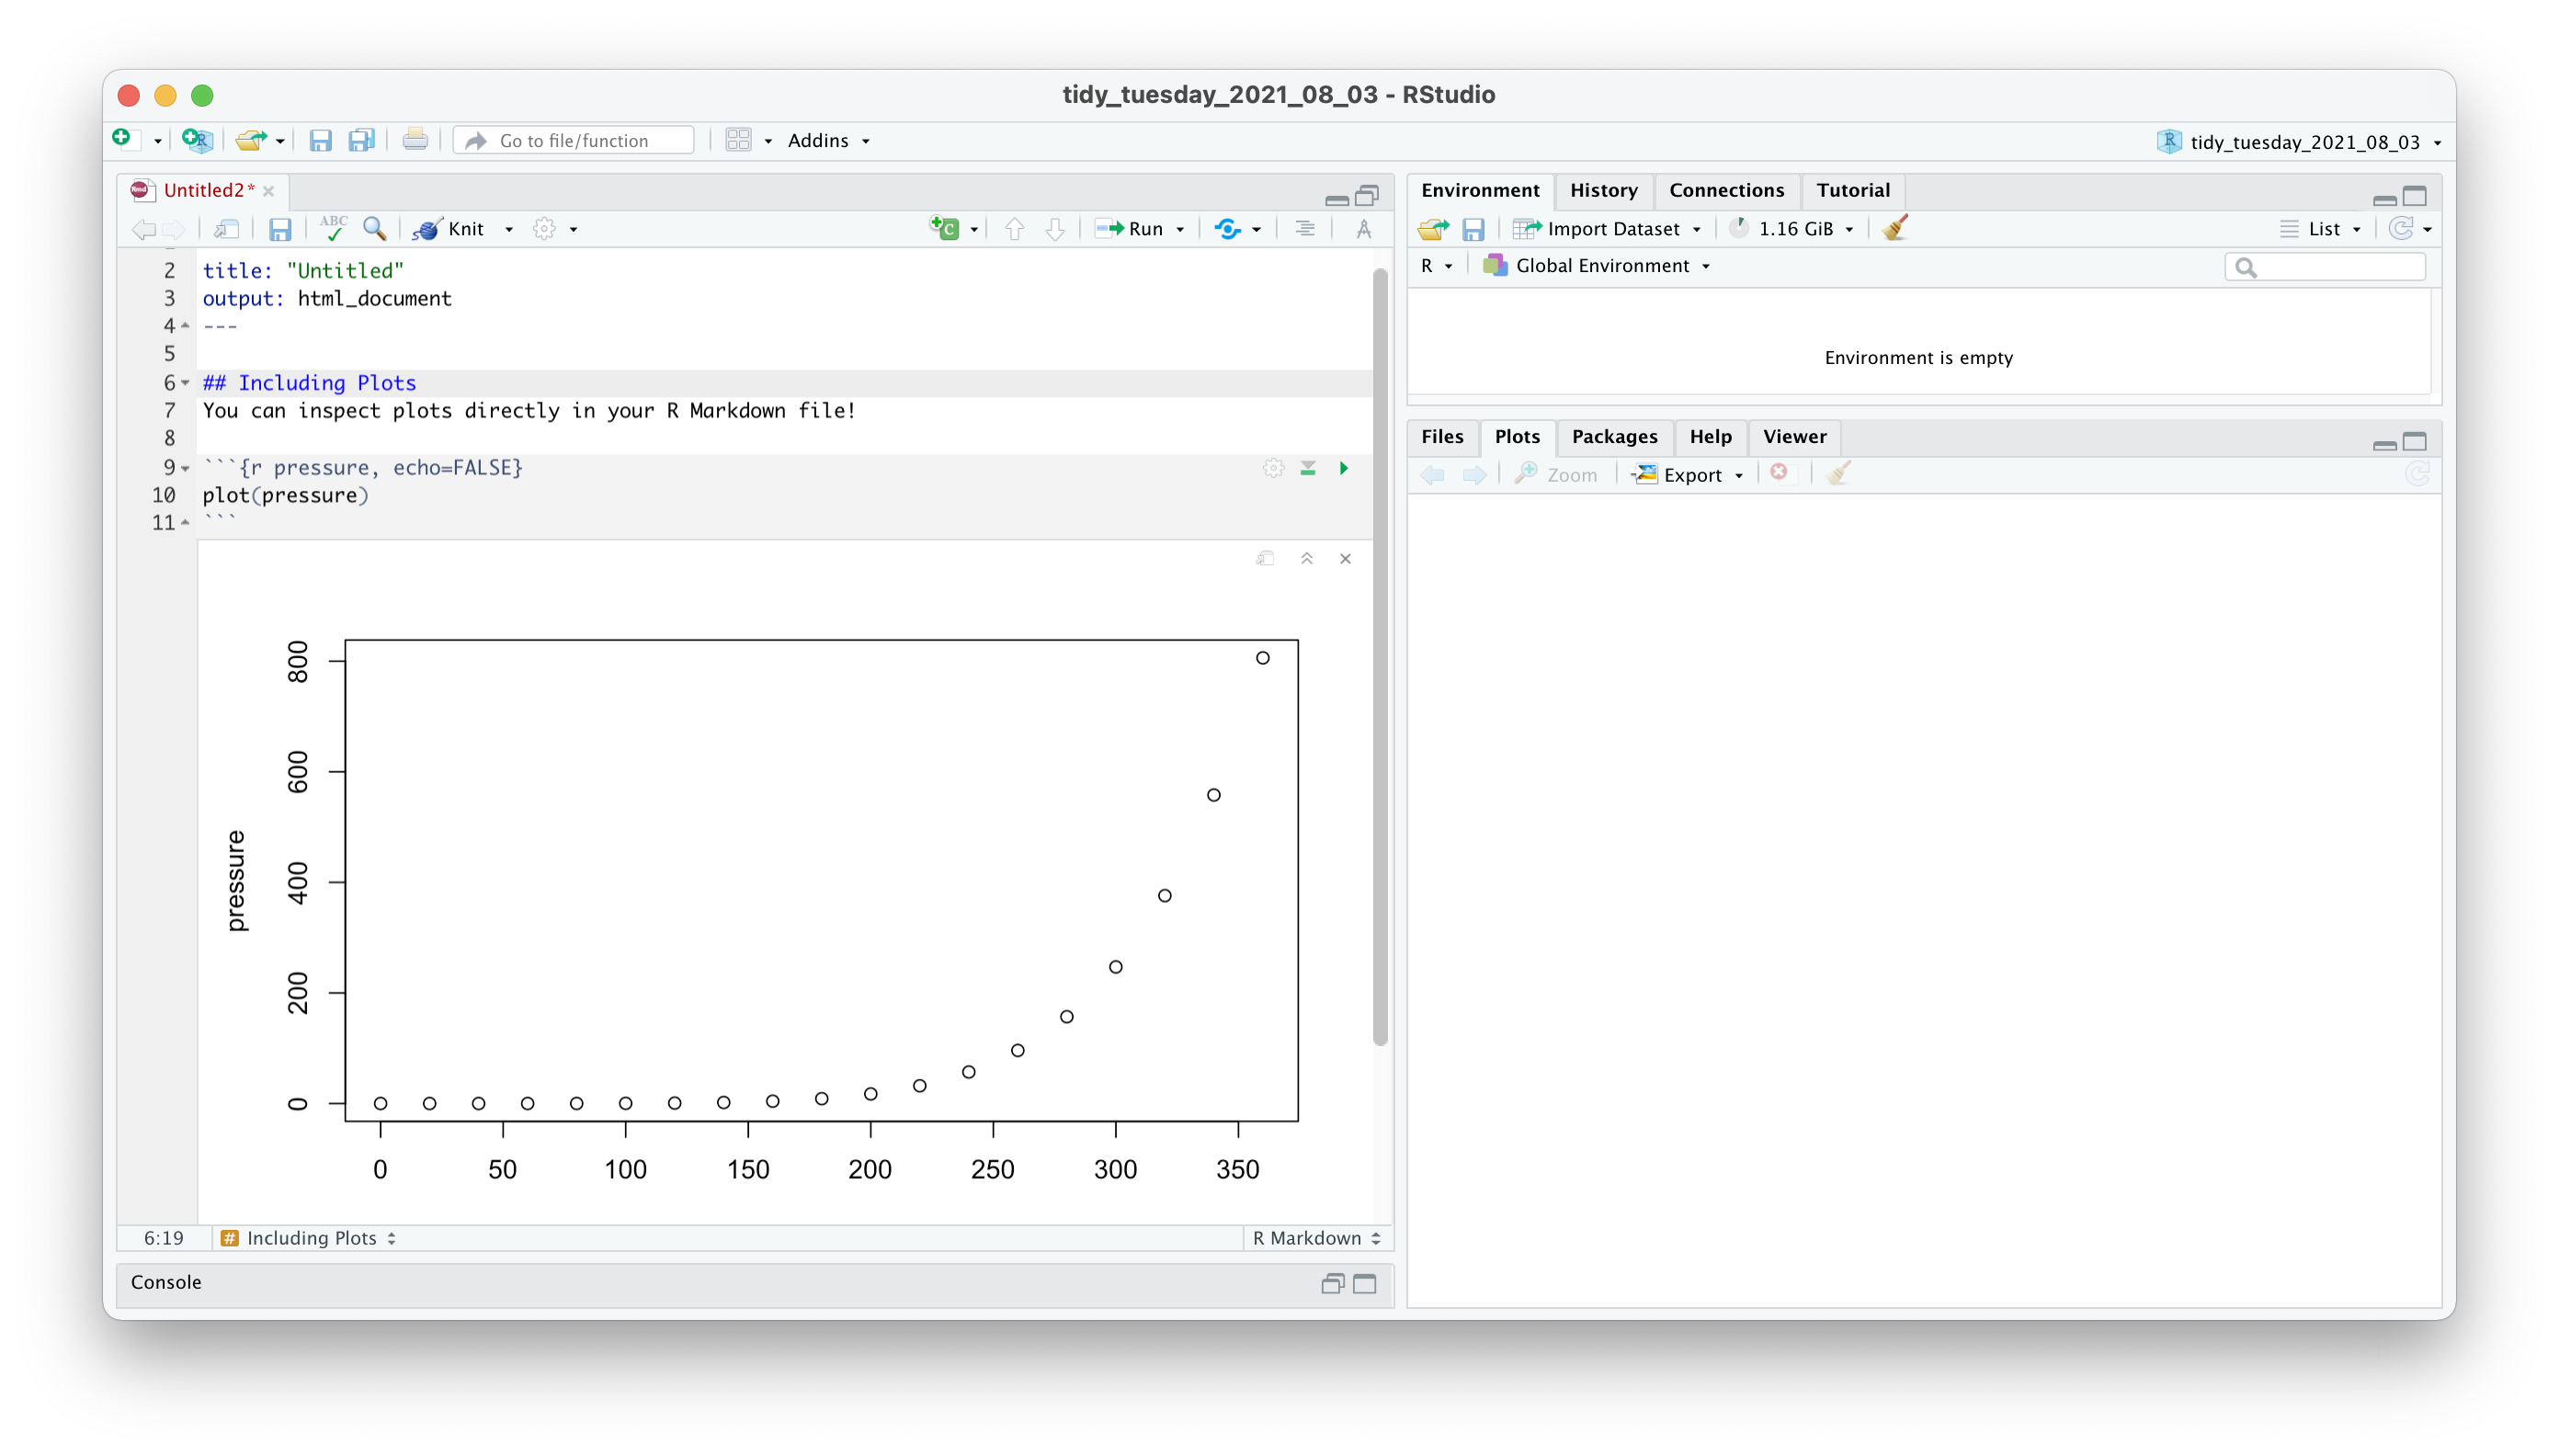
\includegraphics{images/chapter_06_img/03_r_markdown/01_r_markdown_plain.png}

If you switch your view to the \texttt{Visual\ Editor}, it almost looks like you are writing a report in MS Word.

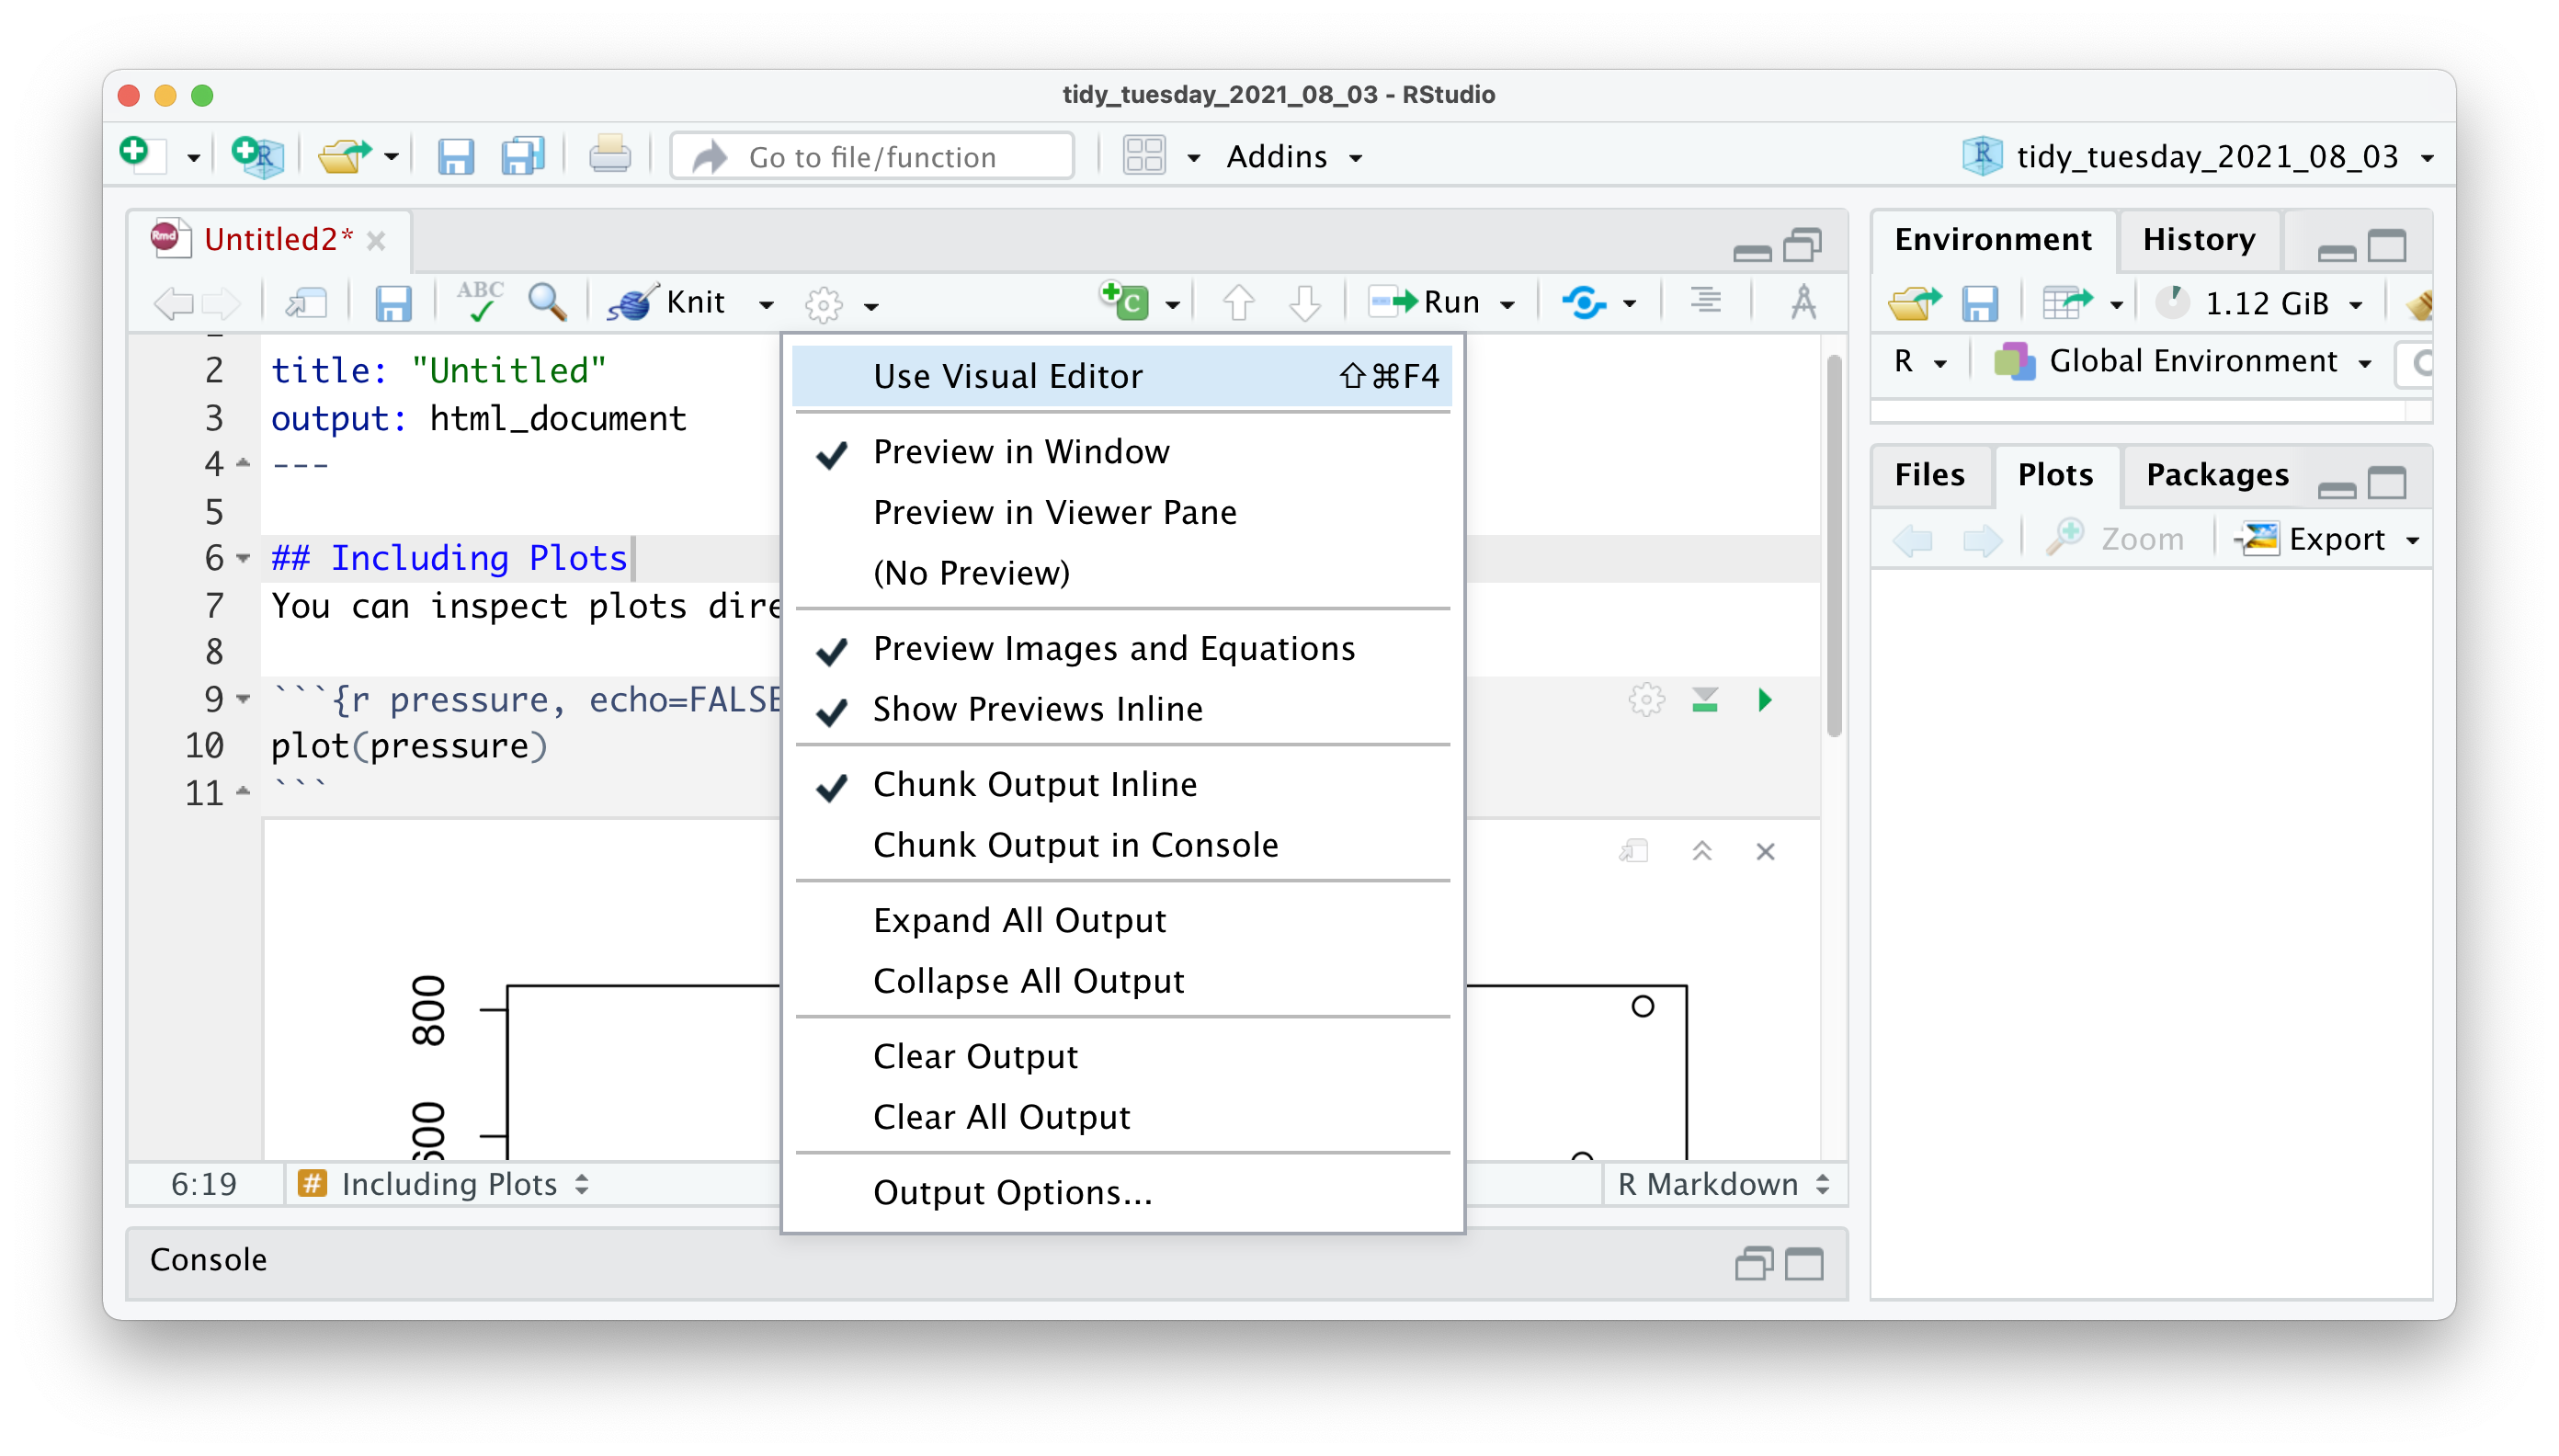
\includegraphics{images/chapter_06_img/03_r_markdown/02_r_markdown_visual_editor_menu.png}

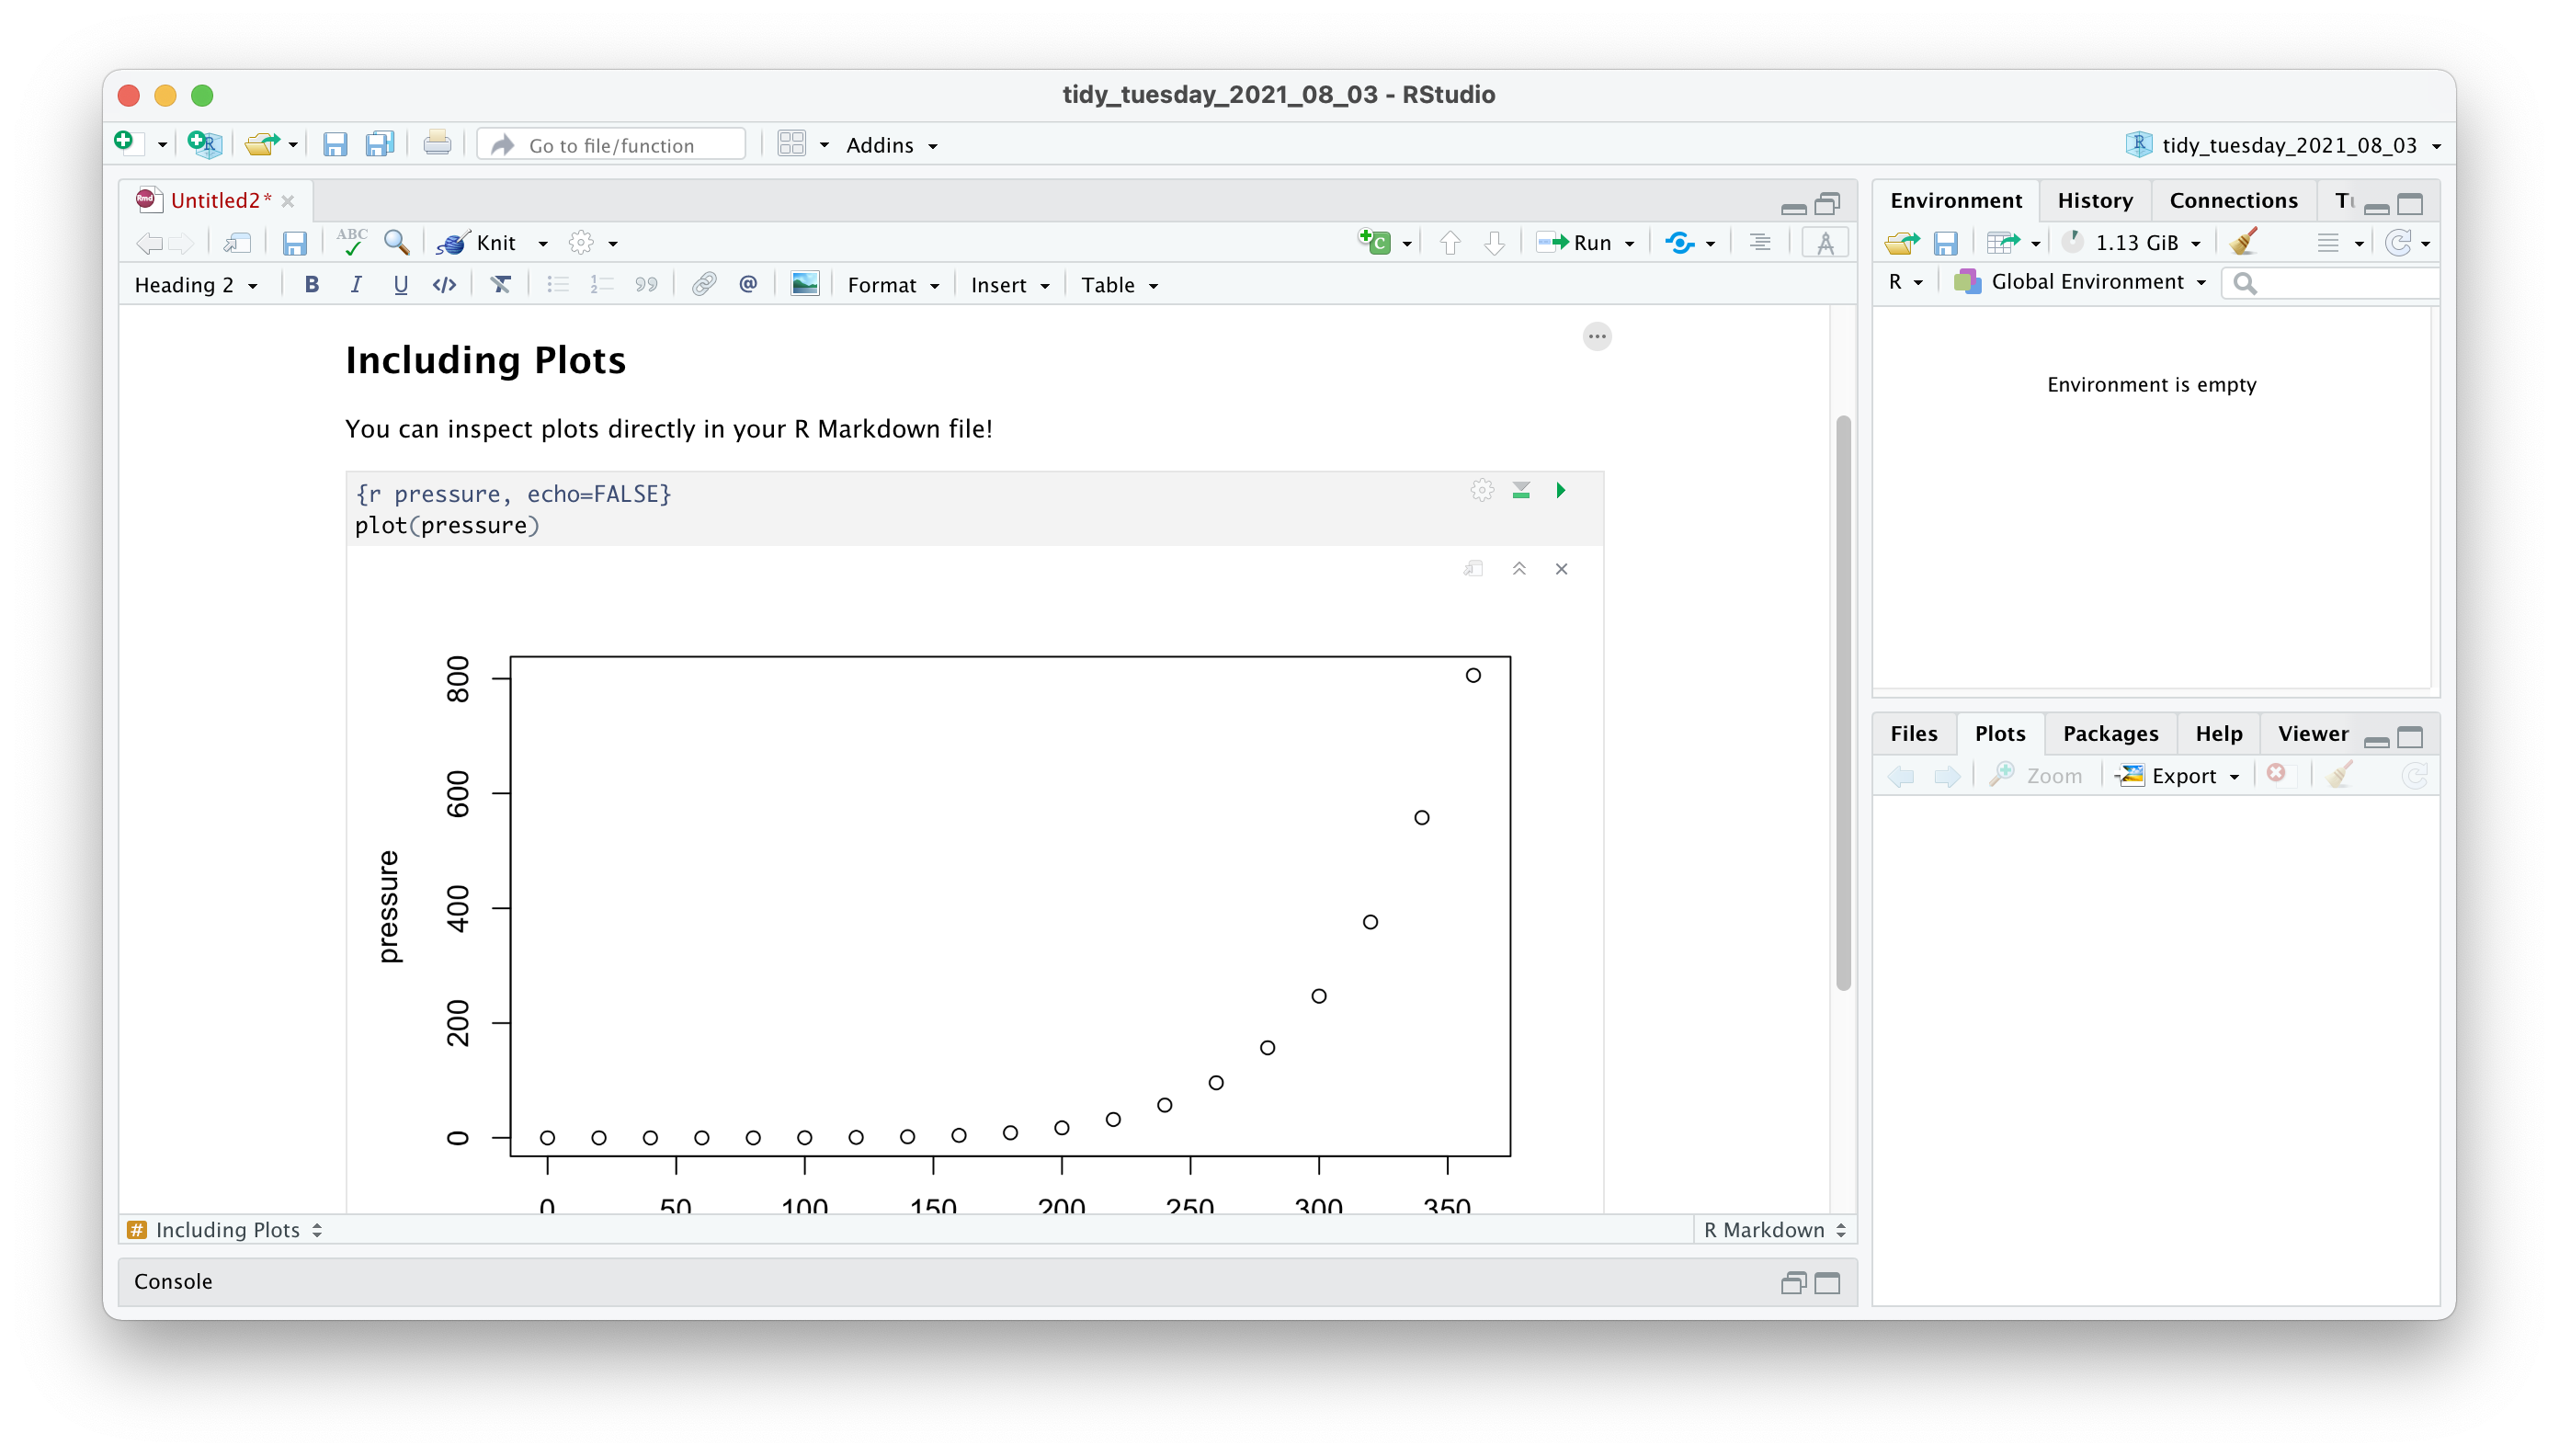
\includegraphics{images/chapter_06_img/03_r_markdown/03_r_markdown_visual_editor.png}

So, when should you use an R Script, and when should you use R Markdown. The rule-of-thumb is that if you intend to write a report, thesis or another form of publication, it might be better to work in an R Markdown file. If this does not apply, you might want to write an R Script. As mentioned above, R Markdown files emphasise text, while R Scripts primarily focus on code. In my projects, I often have a mixture of both. I use R Scripts to carry out data wrangling and my primary analysis and then use R Markdown files to present the findings, e.g.~creating plots, tables, etc. By the way, this book is written in R Markdown using the \texttt{bookdown} package.

No matter your choice, it will neither benefit nor disadvantage you in your R journey or when working through this book. The choice is all yours. You likely will come to appreciate both formats for what they offer. If you want to find out more about R Markdown and how to use it, I highly recommend taking a look at \href{https://bookdown.org/yihui/rmarkdown/}{`R Markdown: The Definitive Guide'} \citep{rmarkdown2018}.

\hypertarget{data-wrangling}{%
\chapter{Data Wrangling}\label{data-wrangling}}

You collected your data over months (and sometimes years), and all you want to know is whether your data makes sense and reveals something nobody would have ever expected. However, before we can truly go ahead with our analysis, it is essential to understand whether our data is `tidy'. Very often, the data we receive is everything else but clean, and we need to check whether our data is fit for analysis and ensure it is in a format that is easy to handle. For small datasets, this is usually a brief exercise. However, I found myself cleaning data for a month because the dataset was spread out into multiple spreadsheets (no pun intended) with different numbers of columns and odd column names. Thus, data cleaning or data wrangling is an essential first step in any data analysis. It is a step that cannot be skipped and has to be performed on every new dataset.

Luckily, R provides many useful functions to make our lives easier. You will be in for a treat if you are like me and used to do this in Excel. It is a lot simpler using R to achieve a clean dataset.

Here is an overview of the different steps we usually work through before starting with our primary analysis. This list is certainly not exhaustive:

\begin{itemize}
\item
  Importing data
\item
  Checking data types
\item
  Recoding and arranging factors, i.e.~categorical data.
\item
  Running missing data diagnostics
\item
  and other things
\end{itemize}

\hypertarget{import-your-data}{%
\section{Import your data}\label{import-your-data}}

The \texttt{r4np} package hosts several different datasets to work with, but at some point, you might want to apply your R knowledge to your own data. Therefore, an essential first step is to import your data into RStudio. There are three different methods, all of which are very handy:

\begin{enumerate}
\def\labelenumi{\arabic{enumi}.}
\item
  Click on your data file in the Files pane and choose \texttt{Import\ Dataset}.
\item
  Use the \texttt{Import\ Dataset} button in the Environment pane.
\item
  Import your data calling one of the \texttt{readr} functions in the console or RScript.
\end{enumerate}

We will use the \texttt{readr} package to import our data. Using this package we can import a range of different file formats, including \texttt{.csv}, \texttt{.tsv}, \texttt{.txt}. If you want to import data from an \texttt{.xlsx} file, you need to use another package called \texttt{readxl}. The following sections will primarily focus on using \texttt{readr} via RStudio or directly in your Console or RScript.

\hypertarget{import-data-from-the-files-pane}{%
\subsection{Import data from the Files pane}\label{import-data-from-the-files-pane}}

This approach is by far the easiest. Let's assume you have a dataset called \texttt{gender\_age.csv} in your \texttt{00\_raw\_data\ folder}. If you wish to import it, you can do the following:

\begin{enumerate}
\def\labelenumi{\arabic{enumi}.}
\item
  Click on the name of the file
\item
  Select \texttt{Import\ Dataset}.

  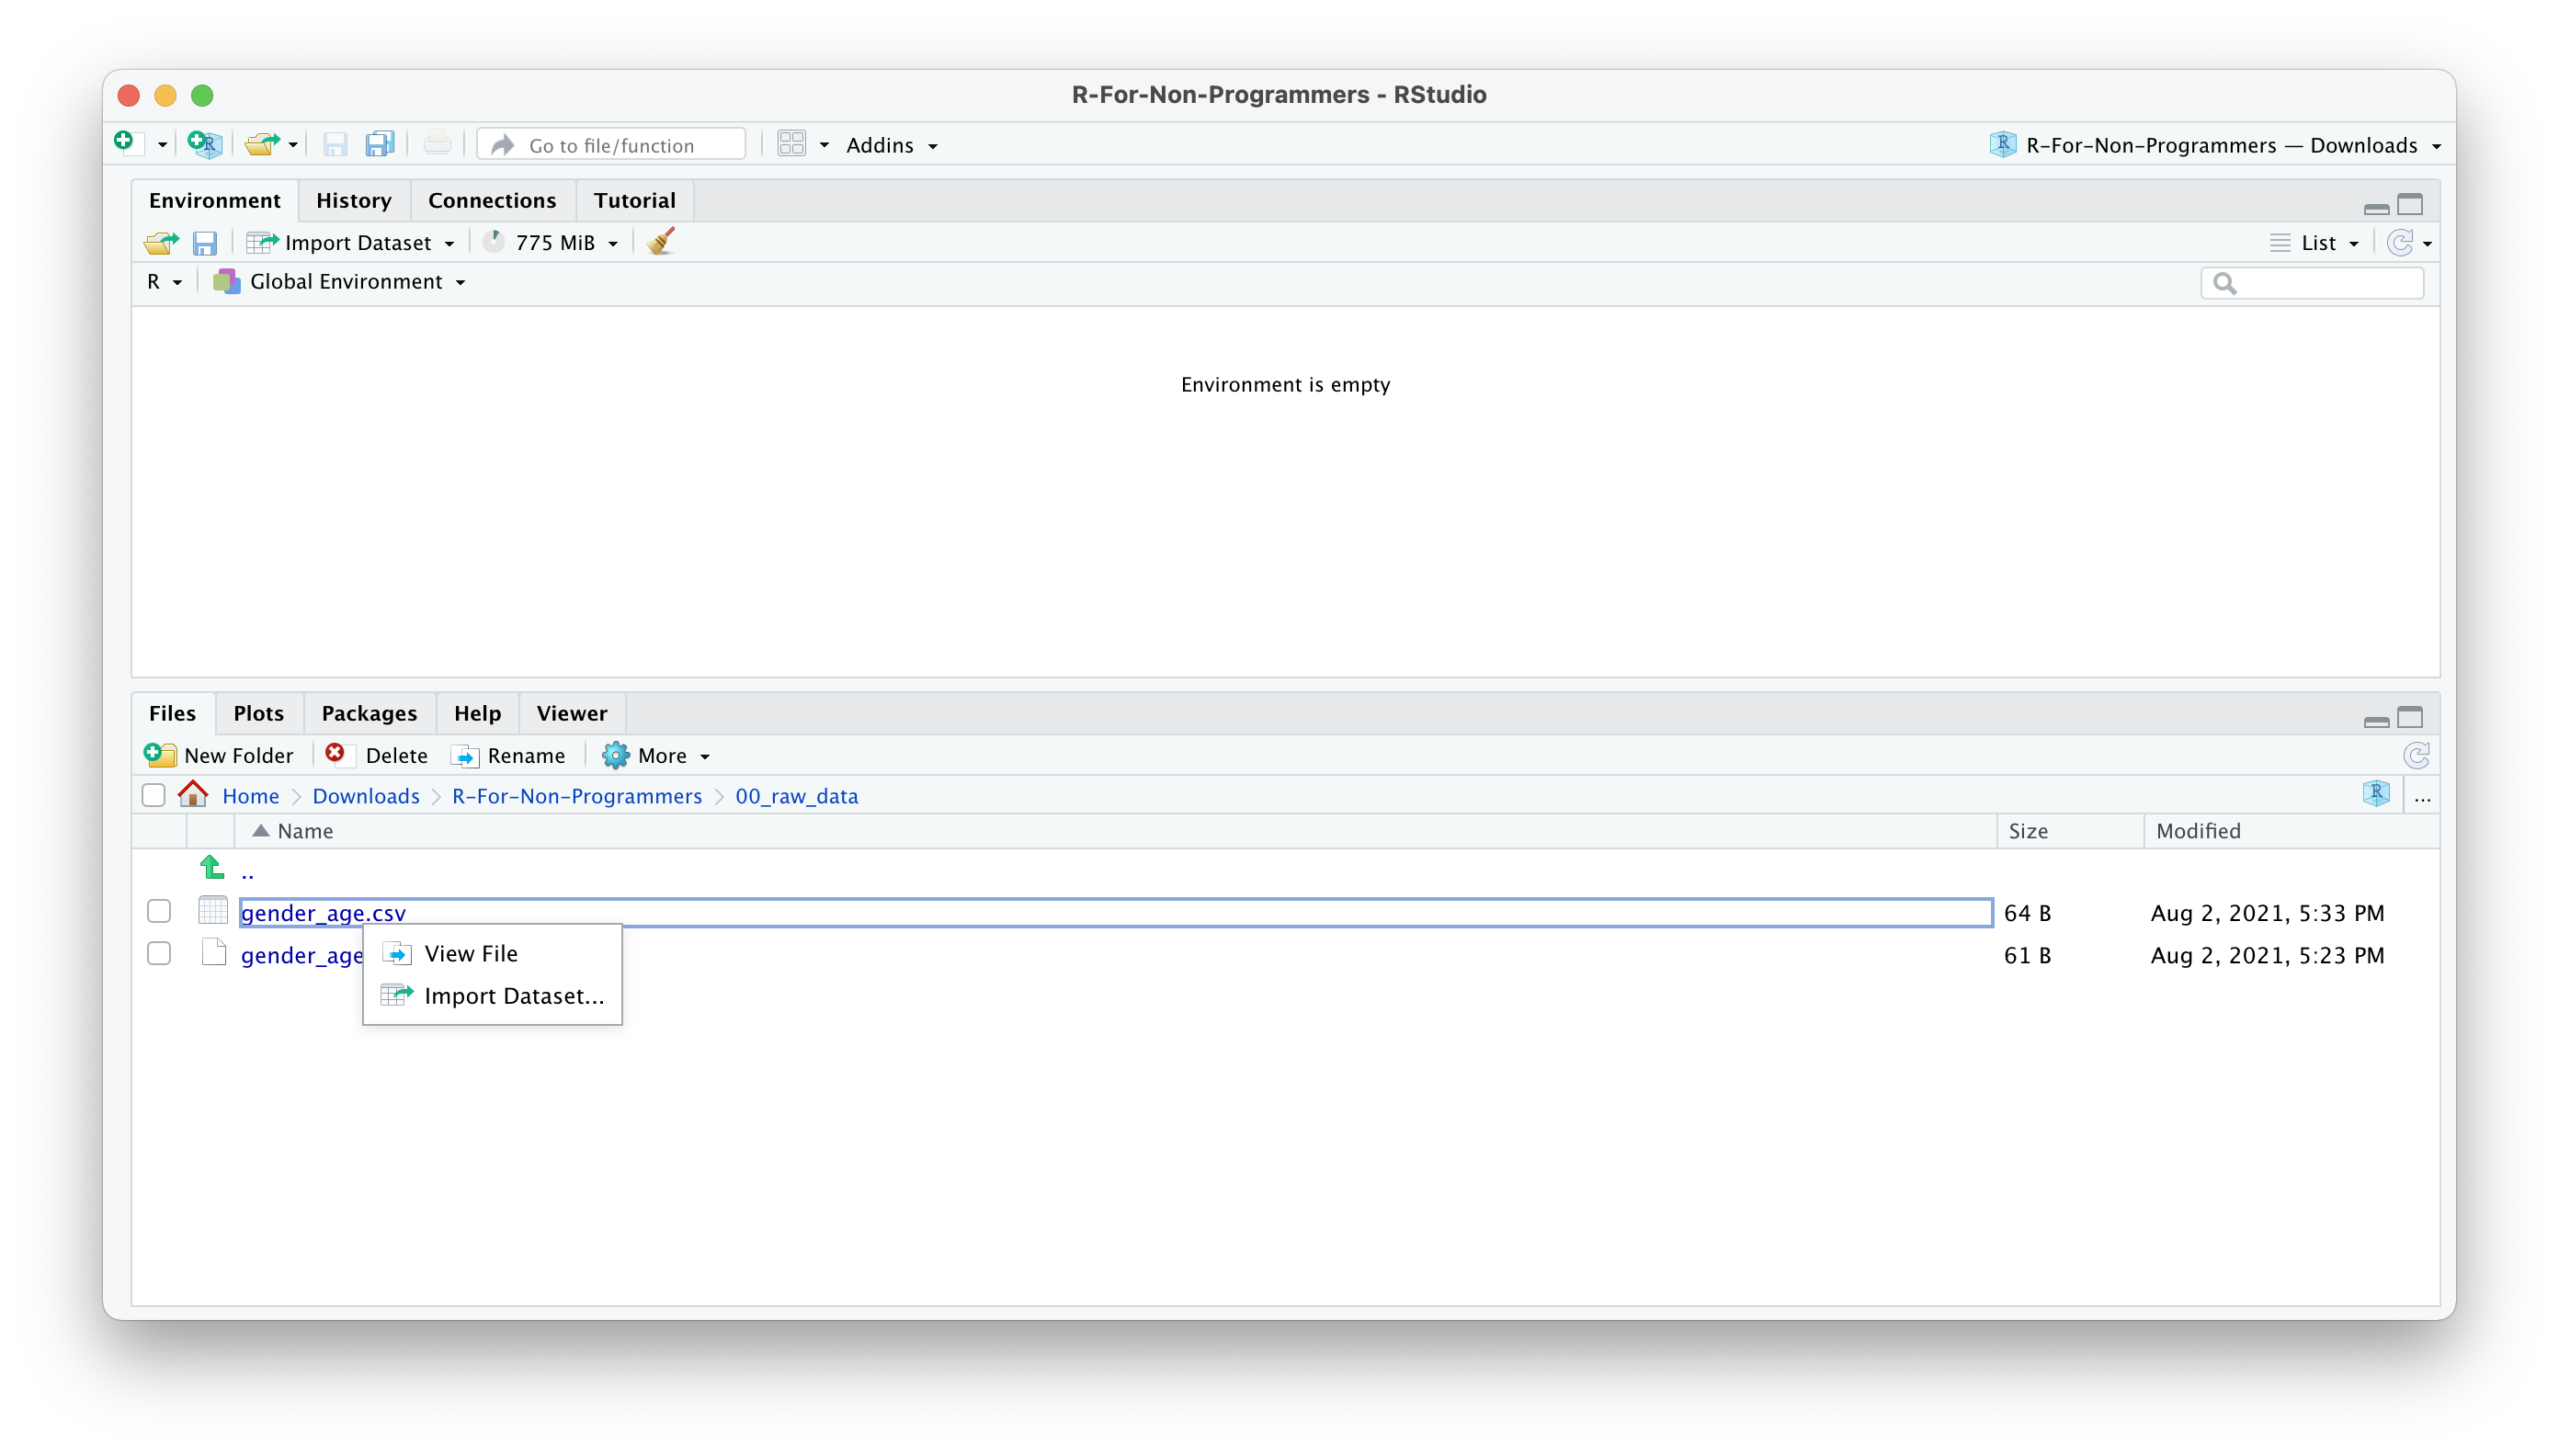
\includegraphics{images/chapter_07_img/01_files_pane_import/01_files_pane_import.png}
\item
  A new window will open, and you can choose different options. You also see a little preview of how the data looks like. This is great if you are not sure whether you did it correctly.

  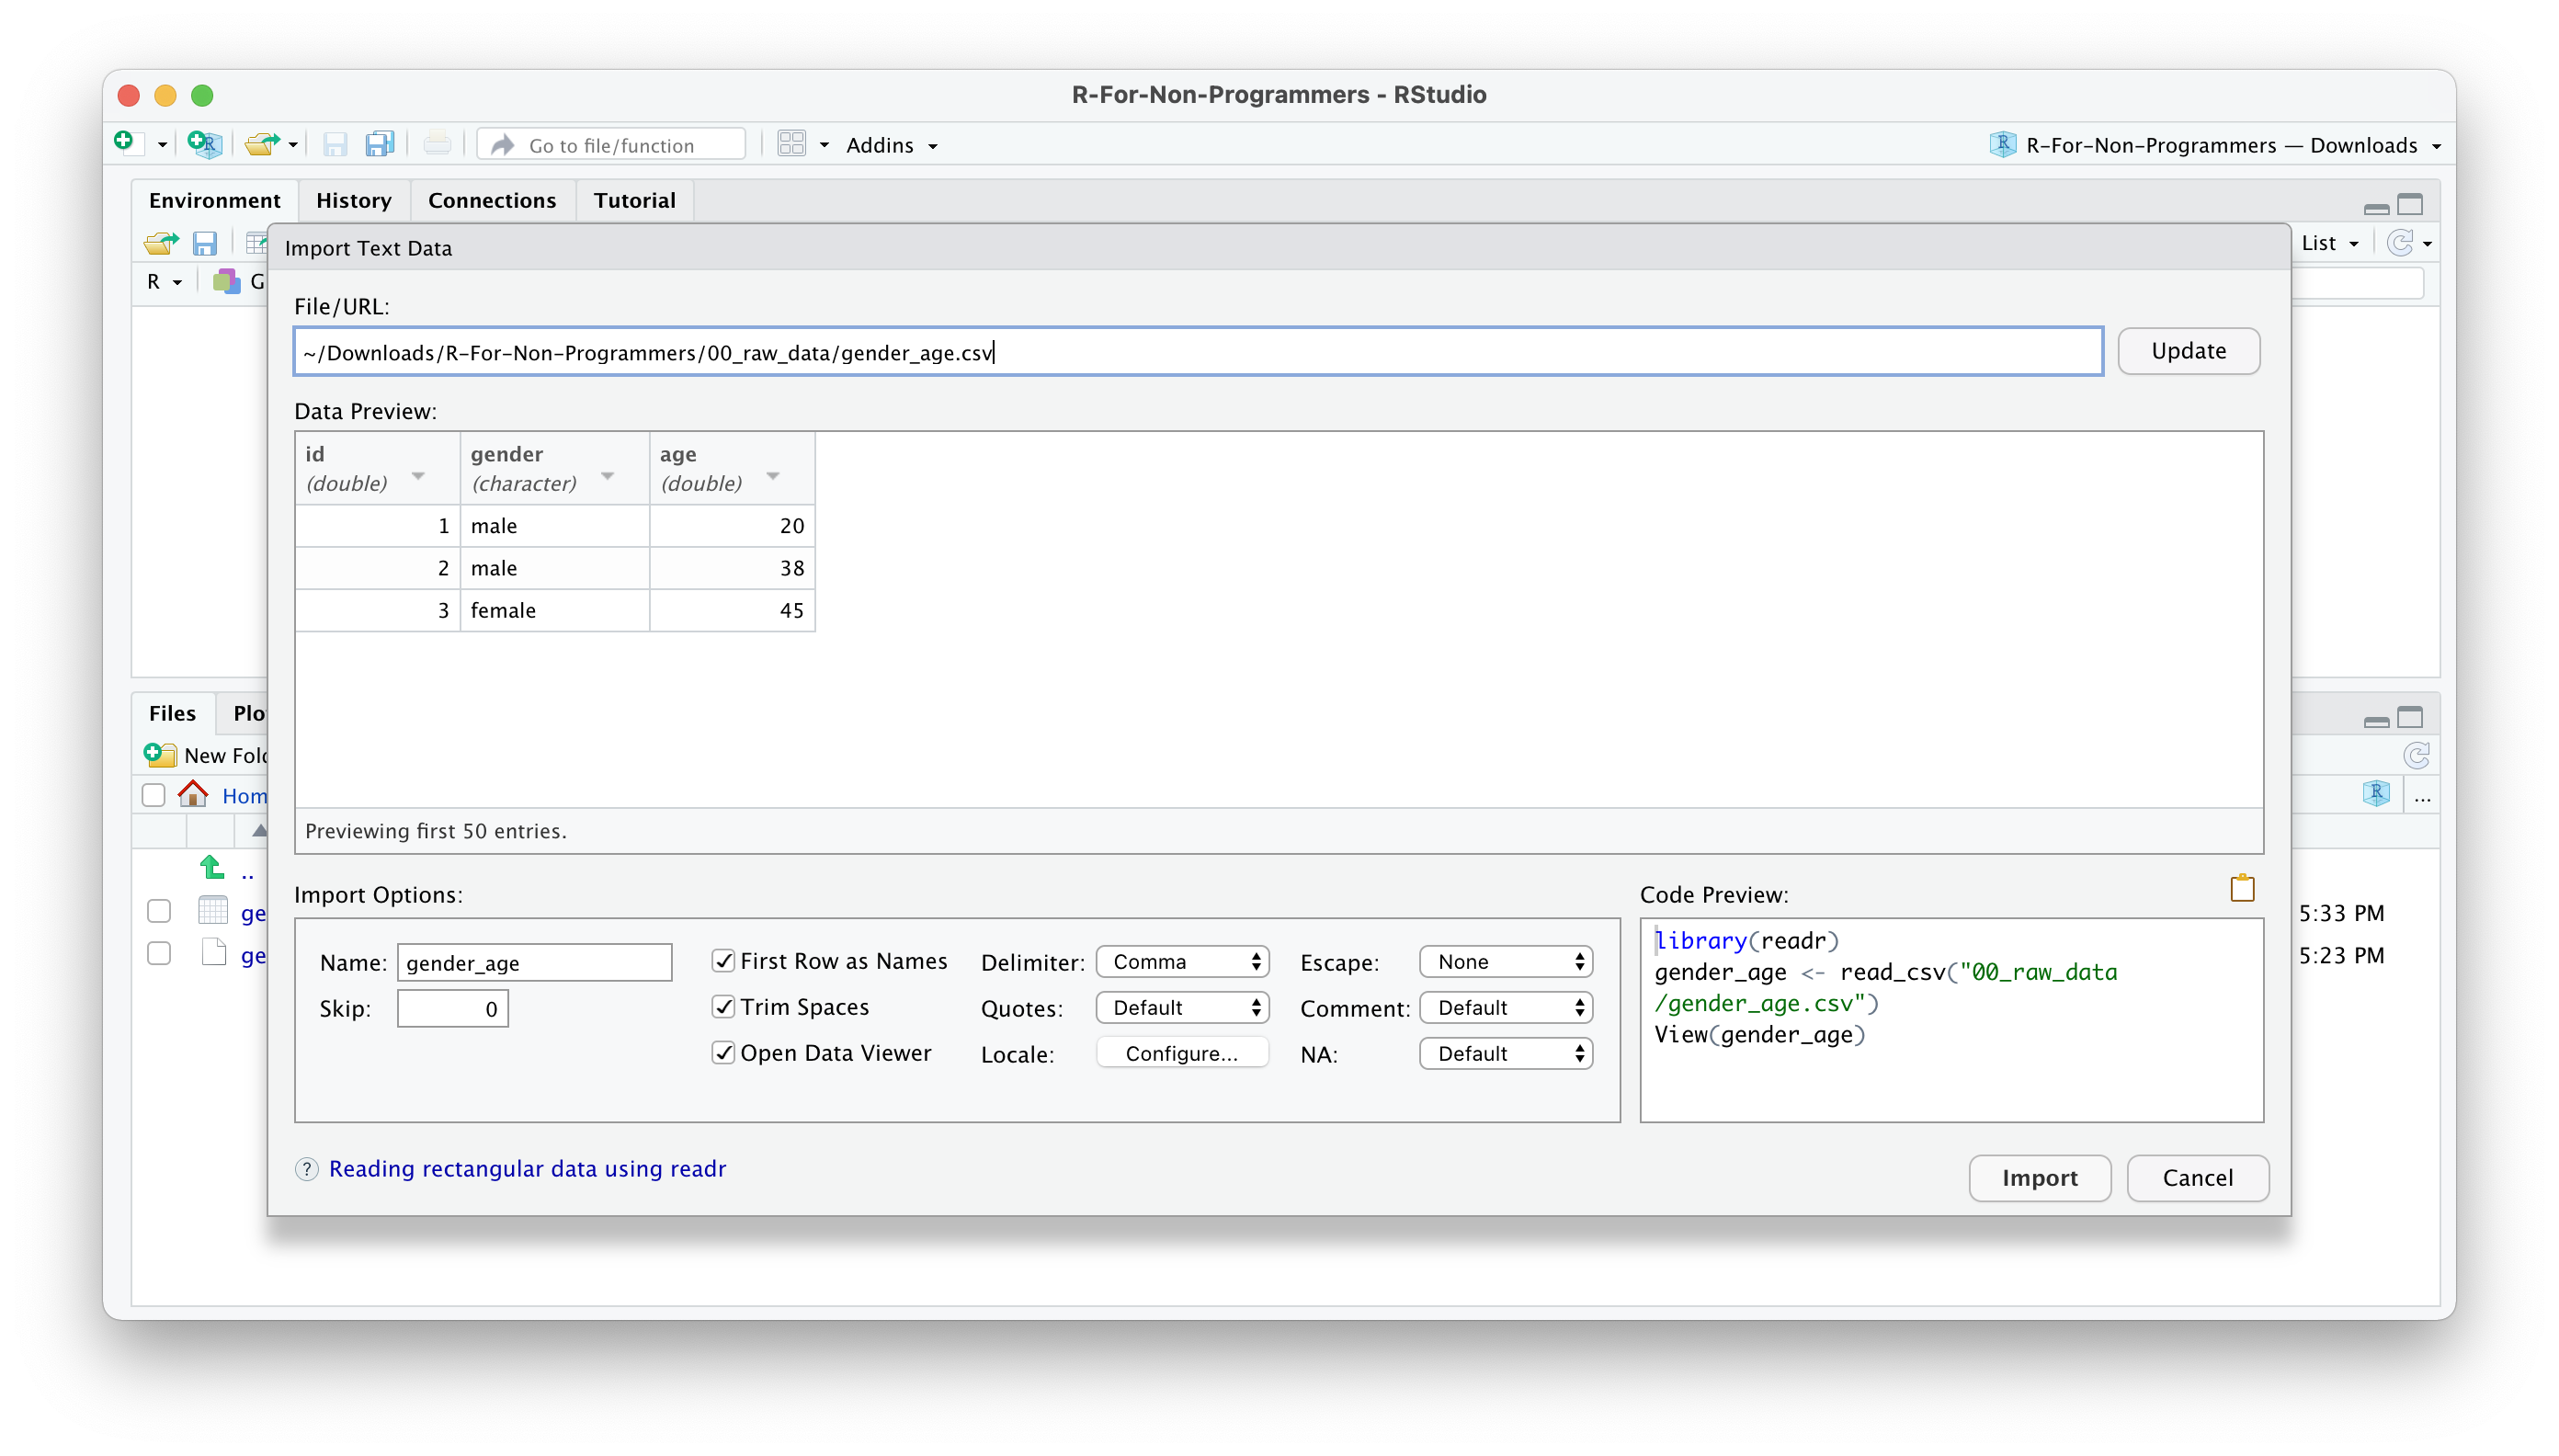
\includegraphics{images/chapter_07_img/01_files_pane_import/02_files_pane_import.png}
\item
  You can change how data should be imported, but the default should be fine in most cases. Here is a quick breakdown of the most important options:

  \begin{itemize}
  \item
    \texttt{Name} allows you to change the object name, i.e.~the name of the object this data will be assigned to. I often use \texttt{df\_raw} (\texttt{df} stand for \texttt{data\ frame}, which is how R calls such rectangular datasets).
  \item
    \texttt{Skip} is helpful if your data file starts with several empty rows at the top. You can remove them here.
  \item
    \texttt{First\ Row\ as\ Names} is ticked by default. In most Social Science projects, we tend to have the name of the variables as the first row in your dataset.
  \item
    \texttt{Trim\ Spaces} removes any unnecessary whitespace in your dataset. Leave it ticked.
  \item
    \texttt{Open\ Data\ Viewer} allows you to look at your imported dataset. I use it rarely, but it can be helpful at times.
  \item
    \texttt{Delimiter} defines how your columns are separate from each other in your file. If it is a \texttt{.csv} it would imply it is a `comma-separated value', i.e.~\texttt{,}. This setting can be changed for different files, depending on how your data is delimited. You can even use the option \texttt{Other\ldots{}} to specify a custom separation option.
  \item
    \texttt{NA} specifies how missing values in your data are acknowledged. By default, empty cells in your data will be recognised as missing data.
  \end{itemize}

  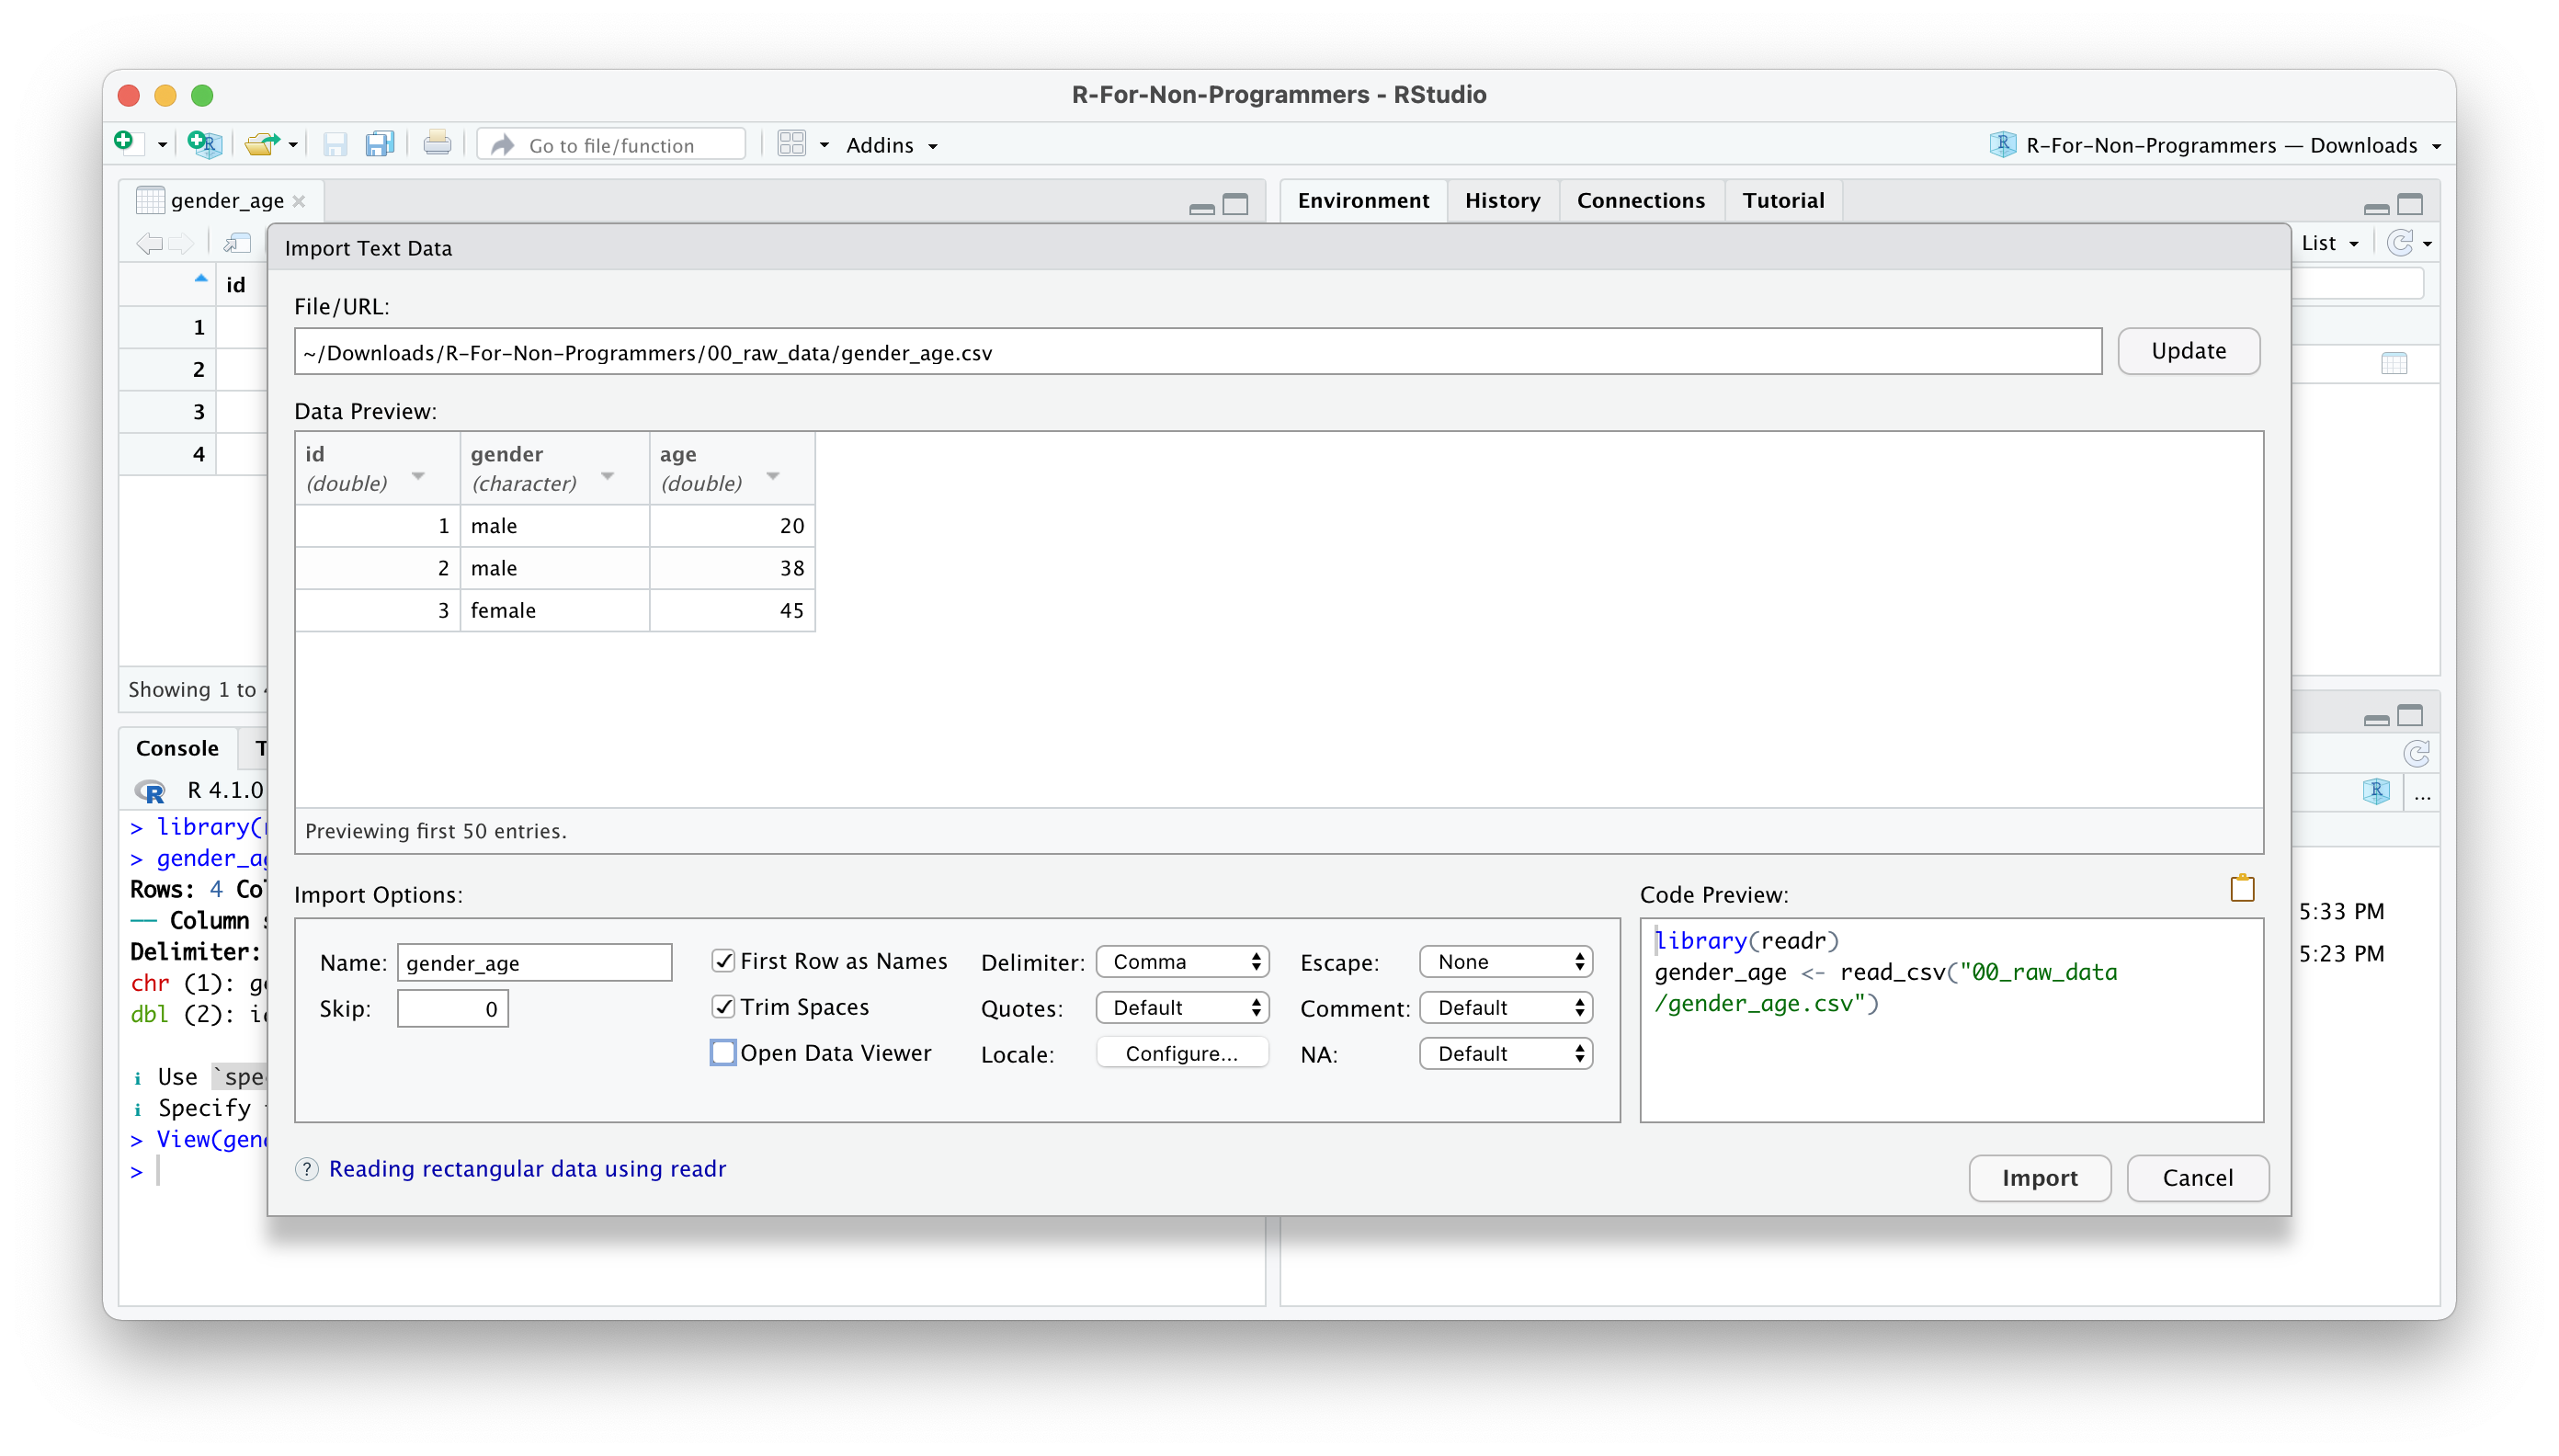
\includegraphics{images/chapter_07_img/01_files_pane_import/03_files_pane_import.png}
\item
  Once you are happy with your choices, you can click on \texttt{Import}.
\item
  You will find your dataset in the Environment pane.

  \includegraphics{images/chapter_07_img/01_files_pane_import/04_files_pane_import.png}
\end{enumerate}

In the Console, you can see that R also provides the \texttt{Column\ specification}, which we need later when inspecting `data types'. \texttt{readr} automatically imports all text-based columns as \texttt{chr}, i.e.~\texttt{character} values. However, this might not always be true. We will cover more of this aspect of data wrangling in Chapter \ref{change-data-types}.

\hypertarget{importing-data-from-the-environment-pane}{%
\subsection{Importing data from the Environment pane}\label{importing-data-from-the-environment-pane}}

The process of importing datasets from the Environment pane follows largely the one from the Files pane. Click on \texttt{Import\ Dataset\ \textgreater{}\ From\ Text\ (readr)\ldots{}}. The only main difference lies in having to find the file using the \texttt{Browse\ldots{}} button. The rest of the steps are the same as above.

You will have to use the Environment pane for importing data from specific file types, e.g.~\texttt{.txt}, because using the File pane would only open the file but not import the data for further processing.

\hypertarget{importing-data-using-functions}{%
\subsection{Importing data using functions directly}\label{importing-data-using-functions}}

If you organised your files well, it could be effortless and quick to use all the functions from \texttt{readr} directly. Here are two examples of how you can use \texttt{readr} to import your data. Make sure you have the \texttt{tidyverse} package loaded.

\begin{Shaded}
\begin{Highlighting}[]
\CommentTok{\# Import data from \textquotesingle{}.csv\textquotesingle{}}
\FunctionTok{read\_csv}\NormalTok{(}\StringTok{"00\_raw\_data/gender\_age.csv"}\NormalTok{)}

\CommentTok{\# Import data from any file text file by defining the separator yourself}
\FunctionTok{read\_delim}\NormalTok{(}\StringTok{"00\_raw\_data/gender\_age.txt"}\NormalTok{, }\AttributeTok{delim =} \StringTok{"|"}\NormalTok{)}
\end{Highlighting}
\end{Shaded}

You might be wondering whether you can use \texttt{read\_delim()} to import \texttt{.csv} files too. The answer is `Yes, you can!'. In contrast to \texttt{read\_delim()}, \texttt{read\_csv()} sets the delimiter to \texttt{,} by default. This is mainly for convenience because \texttt{.csv} files are one of the most popular file formats used to store their data.

You might also be wondering what a `delimiter' is. When you record data in a plain-text file, it is easy to see where a new observation starts and ends because it is defined by a row in your file. However, we also need to tell our software where a new column starts, i.e.~where a cell begins and ends. Consider the following example. We have a file that holds our data which looks like this:

\begin{verbatim}
idagegender
124male
256female
333male
\end{verbatim}

The first row we probably can still decipher as \texttt{id}, \texttt{age}, \texttt{gender}. However, the next row makes it difficult to understand which value represents the \texttt{id} of a participant and which value reflects the \texttt{age} of that participant. Like us, computer software would find it hard too to decide on this ambiguous content. Thus, we need to use delimiters to make it very clear which value belongs to which column. For example, In a \texttt{.csv} file, the data would be separated by a \texttt{,}.

\begin{verbatim}
id,age,gender
1,24,male
2,56,female
3,33,male
\end{verbatim}

Considering our example from above, we could also use \texttt{\textbar{}} as a delimiter.

\begin{verbatim}
id|age|gender
1|24|male
2|56|female
3|33|male
\end{verbatim}

There is a lot more to \texttt{readr} than could be covered in this book. If you want to know more about this R package, I highly recommend looking at the \href{https://readr.tidyverse.org}{readr webpage}.

\hypertarget{inspecting-raw-data}{%
\section{Inspecting your data}\label{inspecting-raw-data}}

For the rest of this chapter, we will use the \texttt{wvs} dataset from the \texttt{r4np} package. However, we do not know much about this dataset, and therefore we cannot ask any research questions worth investigating. Therefore we need to look at what it contains. The first method of inspecting a dataset is to type the name of the object, i.e.~\texttt{wvs}.

\begin{Shaded}
\begin{Highlighting}[]
\CommentTok{\# Ensure you loaded the \textquotesingle{}r4np\textquotesingle{} package first}
\FunctionTok{library}\NormalTok{(r4np)}

\CommentTok{\# Show the data in the console}
\NormalTok{wvs}
\DocumentationTok{\#\# \# A tibble: 69,578 x 7}
\DocumentationTok{\#\#    \textasciigrave{}Participant ID\textasciigrave{} \textasciigrave{}Country name\textasciigrave{} Gender   Age relationship\_status       }
\DocumentationTok{\#\#               \textless{}dbl\textgreater{} \textless{}chr\textgreater{}           \textless{}dbl\textgreater{} \textless{}dbl\textgreater{} \textless{}chr\textgreater{}                     }
\DocumentationTok{\#\#  1         20070001 Andorra             1    60 married                   }
\DocumentationTok{\#\#  2         20070002 Andorra             0    47 living together as married}
\DocumentationTok{\#\#  3         20070003 Andorra             0    48 separated                 }
\DocumentationTok{\#\#  4         20070004 Andorra             1    62 living together as married}
\DocumentationTok{\#\#  5         20070005 Andorra             0    49 living together as married}
\DocumentationTok{\#\#  6         20070006 Andorra             1    51 married                   }
\DocumentationTok{\#\#  7         20070007 Andorra             1    33 married                   }
\DocumentationTok{\#\#  8         20070008 Andorra             0    55 widowed                   }
\DocumentationTok{\#\#  9         20070009 Andorra             1    40 single                    }
\DocumentationTok{\#\# 10         20070010 Andorra             1    38 living together as married}
\DocumentationTok{\#\# \# ... with 69,568 more rows, and 2 more variables: Freedom.of.Choice \textless{}dbl\textgreater{},}
\DocumentationTok{\#\# \#   Satisfaction{-}with{-}life \textless{}dbl\textgreater{}}
\end{Highlighting}
\end{Shaded}

The result is a series of rows and columns. The first information we receive is: \texttt{A\ tibble:\ 69,578\ x\ 9}. This indicates that our dataset has 69,578 observations (i.e.~rows) and 9 columns (i.e.~variables). This rectangular format is the one we encounter most frequently in Social Sciences (and probably beyond). If you ever worked in Microsoft Excel, this format will look familiar.

Even though it might be nice to look at a dataset in this way, it is not particularly useful. Depending on your monitor size, you might only see a small number of columns, and therefore we do not get to see a complete list of all variables. In short, we hardly ever will find much use in inspecting data this way. Luckily other functions can help us.

If you want to see each variable covered in the dataset and their data types, you can use the function \texttt{glimpse()} from the \texttt{dplyr} package (loaded as part of the \texttt{tidyverse} package).

\begin{Shaded}
\begin{Highlighting}[]
\FunctionTok{glimpse}\NormalTok{(wvs)}
\DocumentationTok{\#\# Rows: 69,578}
\DocumentationTok{\#\# Columns: 7}
\DocumentationTok{\#\# $ \textasciigrave{}Participant ID\textasciigrave{}         \textless{}dbl\textgreater{} 20070001, 20070002, 20070003, 20070004, 20070\textasciitilde{}}
\DocumentationTok{\#\# $ \textasciigrave{}Country name\textasciigrave{}           \textless{}chr\textgreater{} "Andorra", "Andorra", "Andorra", "Andorra", "\textasciitilde{}}
\DocumentationTok{\#\# $ Gender                   \textless{}dbl\textgreater{} 1, 0, 0, 1, 0, 1, 1, 0, 1, 1, 0, 0, 1, 1, 1, \textasciitilde{}}
\DocumentationTok{\#\# $ Age                      \textless{}dbl\textgreater{} 60, 47, 48, 62, 49, 51, 33, 55, 40, 38, 54, 3\textasciitilde{}}
\DocumentationTok{\#\# $ relationship\_status      \textless{}chr\textgreater{} "married", "living together as married", "sep\textasciitilde{}}
\DocumentationTok{\#\# $ Freedom.of.Choice        \textless{}dbl\textgreater{} 10, 9, 9, 9, 8, 10, 10, 8, 8, 10, 9, 8, 10, 7\textasciitilde{}}
\DocumentationTok{\#\# $ \textasciigrave{}Satisfaction{-}with{-}life\textasciigrave{} \textless{}dbl\textgreater{} 10, 9, 9, 8, 7, 10, 5, 8, 8, 10, 8, 8, 10, 7,\textasciitilde{}}
\end{Highlighting}
\end{Shaded}

The output of glimpse shows us the name of each column/variable after the \texttt{\$}, for example, \texttt{\textasciigrave{}Participant\ ID\textasciigrave{}}. The \texttt{\$} is used to lookup certain variables in our dataset. For example, if we want to inspect the column \texttt{relationship\_status} only, we could write the following:

\begin{Shaded}
\begin{Highlighting}[]
\NormalTok{wvs}\SpecialCharTok{$}\NormalTok{relationship\_status}
\DocumentationTok{\#\#     [1] "married"                    "living together as married"}
\DocumentationTok{\#\#     [3] "separated"                  "living together as married"}
\DocumentationTok{\#\#     [5] "living together as married" "married"                   }
\DocumentationTok{\#\#     [7] "married"                    "widowed"                   }
\NormalTok{....}
\end{Highlighting}
\end{Shaded}

After the variable name, we find the recognised datatype for each column in \texttt{\textless{}...\textgreater{}}, for example \texttt{\textless{}chr\textgreater{}}. We will return to data types in Chapter \ref{change-data-types}. Lastly, we get samples of the data included. This output is much more helpful.

I use \texttt{glimpse()} very frequently for different purposes, for example:

\begin{itemize}
\item
  to understand what variables are included in a dataset,
\item
  to check the correctness of data types,
\item
  to inspect variable names for typos or unconventional names,
\item
  to look up variable names.
\end{itemize}

There is one more way to inspect your data and receive more information about it by using a specialised R package. The \texttt{skimr} package is excellent in `skimming' your dataset. It provides not only information about variable names and data types but also provides some descriptive statistics. If you installed the \texttt{r4np} package and called the function \texttt{install\_r4np()}, you will have \texttt{skimr} installed already.

\begin{Shaded}
\begin{Highlighting}[]
\NormalTok{skimr}\SpecialCharTok{::}\FunctionTok{skim}\NormalTok{(wvs)}
\end{Highlighting}
\end{Shaded}

The output in the Console should look like this:

\includegraphics{images/chapter_07_img/02_skimr_output/skimr_output.png}

As you can tell, there is a lot more information in this output. Many descriptive statistics that could be useful are already displayed. \texttt{skim()} provides a summary of the dataset and then automatically sorts the variables by data type. Depending on the data type, you also receive different descriptive statistics. As a bonus, the function also provides a histogram for numeric variables. However, there is one main problem: Some of the numeric variables are not numeric: \texttt{Participant\ ID} and \texttt{Gender}. Thus, we will have to correct the data types in a moment.

Inspecting your data in this way can be helpful to get a better understanding of what your data includes and spot problems with it. In addition, if you receive data from someone else, these methods are an excellent way to familiarise yourself with the dataset relatively quickly. Since I prepared this particular dataset for this book, I also made sure to provide documentation for it. You can access it by using \texttt{?wvs} in the Console. This will open the documentation in the Help pane. Such documentation is available for every dataset we use in this book.

\hypertarget{colnames-cleaning}{%
\section{\texorpdfstring{Cleaning your column names: Call the \texttt{janitor}}{Cleaning your column names: Call the janitor}}\label{colnames-cleaning}}

If you have an eagle eye, you might have noticed that most of the variable names in \texttt{wvs} are not consistent or easy to read/use.

\hypertarget{messy_column_names}{%
\label{messy_column_names}}%
\begin{Shaded}
\begin{Highlighting}[]
\CommentTok{\# Whitespace and inconsistent capitalisation}
\NormalTok{Participant ID        }
\NormalTok{Country name          }
\NormalTok{Gender                }
\NormalTok{Age                   }

\CommentTok{\# Difficult to read}
\NormalTok{YearOfBirth           }
\NormalTok{Freedom.of.Choice     }
\NormalTok{Satisfaction}\SpecialCharTok{{-}}\NormalTok{with}\SpecialCharTok{{-}}\NormalTok{life}
\end{Highlighting}
\end{Shaded}

From Chapter \ref{coding-etiquette}, you will remember that being consistent in writing your code and naming your objects is essential. The same applies, of course, to variable names. R will not break using the existing names, but it will save you a lot of frustration if we take a minute to clean the names and make them more consistent.

You are probably thinking: ``This is easy. I just open the dataset in Excel and change all the column names.'' Indeed, it would be a viable and easy option, but it is not very efficient, especially with larger datasets with many more variables. Instead, we can make use of the \texttt{janitor} package. By definition, \texttt{janitor} is a package that helps to clean up whatever needs cleaning. In our case, we want to tidy our column names. We can use the function \texttt{clean\_names()} to achieve this. We store the result in a new object called \texttt{wvs} to keep those changes. The object will also show up in our Environment pane.

\begin{Shaded}
\begin{Highlighting}[]
\NormalTok{wvs }\OtherTok{\textless{}{-}}\NormalTok{ janitor}\SpecialCharTok{::}\FunctionTok{clean\_names}\NormalTok{(wvs)}
\FunctionTok{glimpse}\NormalTok{(wvs)}
\DocumentationTok{\#\# Rows: 69,578}
\DocumentationTok{\#\# Columns: 7}
\DocumentationTok{\#\# $ participant\_id         \textless{}dbl\textgreater{} 20070001, 20070002, 20070003, 20070004, 2007000\textasciitilde{}}
\DocumentationTok{\#\# $ country\_name           \textless{}chr\textgreater{} "Andorra", "Andorra", "Andorra", "Andorra", "An\textasciitilde{}}
\DocumentationTok{\#\# $ gender                 \textless{}dbl\textgreater{} 1, 0, 0, 1, 0, 1, 1, 0, 1, 1, 0, 0, 1, 1, 1, 0,\textasciitilde{}}
\DocumentationTok{\#\# $ age                    \textless{}dbl\textgreater{} 60, 47, 48, 62, 49, 51, 33, 55, 40, 38, 54, 39,\textasciitilde{}}
\DocumentationTok{\#\# $ relationship\_status    \textless{}chr\textgreater{} "married", "living together as married", "separ\textasciitilde{}}
\DocumentationTok{\#\# $ freedom\_of\_choice      \textless{}dbl\textgreater{} 10, 9, 9, 9, 8, 10, 10, 8, 8, 10, 9, 8, 10, 7, \textasciitilde{}}
\DocumentationTok{\#\# $ satisfaction\_with\_life \textless{}dbl\textgreater{} 10, 9, 9, 8, 7, 10, 5, 8, 8, 10, 8, 8, 10, 7, 1\textasciitilde{}}
\end{Highlighting}
\end{Shaded}

Now that \texttt{janitor} has done its magic, we suddenly have easy to read variable names that are consistent with the `Tidyverse style guide' \citep{wickham-2021}.

If for whatever reason, the variable names are still not looking the way you want, you can use the function \texttt{rename()} from the \texttt{dplyr} package to manually assign new variable names.

\begin{Shaded}
\begin{Highlighting}[]
\NormalTok{wvs }\OtherTok{\textless{}{-}}\NormalTok{ wvs }\SpecialCharTok{\%\textgreater{}\%} \FunctionTok{rename}\NormalTok{(}\AttributeTok{satisfaction =}\NormalTok{ satisfaction\_with\_life,}
                      \AttributeTok{country =}\NormalTok{ country\_name)}
\FunctionTok{glimpse}\NormalTok{(wvs)}
\DocumentationTok{\#\# Rows: 69,578}
\DocumentationTok{\#\# Columns: 7}
\DocumentationTok{\#\# $ participant\_id      \textless{}dbl\textgreater{} 20070001, 20070002, 20070003, 20070004, 20070005, \textasciitilde{}}
\DocumentationTok{\#\# $ country             \textless{}chr\textgreater{} "Andorra", "Andorra", "Andorra", "Andorra", "Andor\textasciitilde{}}
\DocumentationTok{\#\# $ gender              \textless{}dbl\textgreater{} 1, 0, 0, 1, 0, 1, 1, 0, 1, 1, 0, 0, 1, 1, 1, 0, 0,\textasciitilde{}}
\DocumentationTok{\#\# $ age                 \textless{}dbl\textgreater{} 60, 47, 48, 62, 49, 51, 33, 55, 40, 38, 54, 39, 44\textasciitilde{}}
\DocumentationTok{\#\# $ relationship\_status \textless{}chr\textgreater{} "married", "living together as married", "separate\textasciitilde{}}
\DocumentationTok{\#\# $ freedom\_of\_choice   \textless{}dbl\textgreater{} 10, 9, 9, 9, 8, 10, 10, 8, 8, 10, 9, 8, 10, 7, 10,\textasciitilde{}}
\DocumentationTok{\#\# $ satisfaction        \textless{}dbl\textgreater{} 10, 9, 9, 8, 7, 10, 5, 8, 8, 10, 8, 8, 10, 7, 10, \textasciitilde{}}
\end{Highlighting}
\end{Shaded}

You are probably wondering what \texttt{\%\textgreater{}\%} stands for. This symbol is called a \emph{`piping operator'} , and it allows us to chain multiple functions together by considering the output of the previous function. So, do not confuse \texttt{\textless{}-} with \texttt{\%\textgreater{}\%}. Each operator serves a different purpose. The \texttt{\%\textgreater{}\%} has become synonymous with the \texttt{tidyverse} approach to R programming and is the chosen approach for this book. Many functions from the \texttt{tidyverse} are designed to be chained together.

If we wanted to spell out what we just did, we could say:

\begin{enumerate}
\def\labelenumi{\arabic{enumi}.}
\item
  \texttt{wvs\ \textless{}-}: We assigned whatever happened to the right of the assignment operator to the object \texttt{wvs}.
\item
  \texttt{wvs\ \%\textgreater{}\%}: We defined the dataset we want to use with the functions defined after the \texttt{\%\textgreater{}\%}.
\item
  \texttt{rename(satisfaction\ =\ satisfcation\_with\_life)}: We define a new name \texttt{satisfaction} for the column \texttt{satisfaction\_with\_life}. Notice that the order is \texttt{new\_name\ =\ old\_name}. Here we also use \texttt{=}. A rare occasion where it makes sense to do so.
\end{enumerate}

Just for clarification, the following two lines of code accomplish the same task. The only difference lies that with \texttt{\%\textgreater{}\%} we could chain another function right after it. So, you could say, it is a matter of taste which approach you prefer. However, in later chapters, it will become apparent why using \texttt{\%\textgreater{}\%} is very advantageous.

\begin{Shaded}
\begin{Highlighting}[]
\CommentTok{\# Renaming a column using \textquotesingle{}\%\textgreater{}\%\textquotesingle{}}
\NormalTok{wvs }\SpecialCharTok{\%\textgreater{}\%} \FunctionTok{rename}\NormalTok{(}\AttributeTok{satisfaction\_new =}\NormalTok{ satisfaction)}

\CommentTok{\# Renaming a column without \textquotesingle{}\%\textgreater{}\%\textquotesingle{}}
\FunctionTok{rename}\NormalTok{(wvs, }\AttributeTok{satisfaction\_new =}\NormalTok{ satisfaction)}
\end{Highlighting}
\end{Shaded}

Since you will be using the pipe operator very frequently, it is a good idea to remember the keyboard shortcut for it: \texttt{Ctrl+Shift+M} for PC and \texttt{Cmd+Shift+M} for Mac.

\hypertarget{change-data-types}{%
\section{Data types: What are they and how can you change them}\label{change-data-types}}

When we inspected our data, I mentioned that some variables do not have the correct data type. You might be familiar with different data types by classifying them as:

\begin{itemize}
\item
  \emph{Nominal data}, which is categorical data of no particular order,
\item
  \emph{Ordinal data}, which is categorical data with a defined order, and
\item
  \emph{Quantitative data}, which is data that usually is represented by numeric values.
\end{itemize}

In R we have a slightly different distinction:

\begin{itemize}
\item
  \texttt{character} / \texttt{\textless{}chr\textgreater{}}: Textual data, for example the text of a tweet.
\item
  \texttt{factor} / \texttt{\textless{}fct\textgreater{}}: Categorical data with a finite number of categories with no particular order.
\item
  \texttt{ordered} / \texttt{\textless{}ord\textgreater{}}: Categorical data with a finite number of categories with a particular order.
\item
  \texttt{double} / \texttt{\textless{}dbl\textgreater{}}: Numerical data with decimal places.
\item
  \texttt{integer} / \texttt{\textless{}int\textgreater{}}: Numerical data with whole numbers only (i.e.~no decimals).
\item
  \texttt{logical} / \texttt{\textless{}lgl\textgreater{}}: Logical data, which only consists of values `TRUE' and `FALSE'.
\item
  \texttt{date} / \texttt{date}: Data which consists dates, e.g.~`2021-08-05'.
\item
  \texttt{date-time} / \texttt{dttm}: Data which consists dates and times, e.g.~`2021-08-05 16:29:25 BST'.
\end{itemize}

For a complete list of data types, I recommend looking at \href{https://tibble.tidyverse.org/articles/types.html}{`Column Data Types'} \citep{data-types-2021}.

R has a more fine-grained categorisation of data types. The most important distinction, though, lies between \texttt{\textless{}chr\textgreater{}}, \texttt{\textless{}fct\textgreater{}}/\texttt{\textless{}ord\textgreater{}} and \texttt{\textless{}dbl\textgreater{}} for most datasets in the Social Sciences. Still, it is good to know what the abbreviations in your \texttt{tibble} mean and how they might affect your analysis.

Now that we have a solid understanding of different data types, we can look at our dataset and see whether \texttt{readr} classified our variables correctly.

\begin{Shaded}
\begin{Highlighting}[]
\FunctionTok{glimpse}\NormalTok{(wvs)}
\DocumentationTok{\#\# Rows: 69,578}
\DocumentationTok{\#\# Columns: 7}
\DocumentationTok{\#\# $ participant\_id      \textless{}dbl\textgreater{} 20070001, 20070002, 20070003, 20070004, 20070005, \textasciitilde{}}
\DocumentationTok{\#\# $ country             \textless{}chr\textgreater{} "Andorra", "Andorra", "Andorra", "Andorra", "Andor\textasciitilde{}}
\DocumentationTok{\#\# $ gender              \textless{}dbl\textgreater{} 1, 0, 0, 1, 0, 1, 1, 0, 1, 1, 0, 0, 1, 1, 1, 0, 0,\textasciitilde{}}
\DocumentationTok{\#\# $ age                 \textless{}dbl\textgreater{} 60, 47, 48, 62, 49, 51, 33, 55, 40, 38, 54, 39, 44\textasciitilde{}}
\DocumentationTok{\#\# $ relationship\_status \textless{}chr\textgreater{} "married", "living together as married", "separate\textasciitilde{}}
\DocumentationTok{\#\# $ freedom\_of\_choice   \textless{}dbl\textgreater{} 10, 9, 9, 9, 8, 10, 10, 8, 8, 10, 9, 8, 10, 7, 10,\textasciitilde{}}
\DocumentationTok{\#\# $ satisfaction        \textless{}dbl\textgreater{} 10, 9, 9, 8, 7, 10, 5, 8, 8, 10, 8, 8, 10, 7, 10, \textasciitilde{}}
\end{Highlighting}
\end{Shaded}

\texttt{readr} did a great job in identifying all the numeric variables. However, by default, \texttt{readr} imports all variables that include text as \texttt{\textless{}chr\textgreater{}}. It appears, in our dataset, this is not entirely correct. The variables \texttt{country}, \texttt{gender} and \texttt{relationship\_status} specify a finite number of categories. Therefore they should be classified as a \texttt{factor}. The variable \texttt{participant\_id} is represented by numbers, but its meaning is also rather categorical. We would not use the ID numbers of participants to perform additions or multiplications. This would make no sense. Therefore, it might be wise to turn them into a \texttt{factor}, even though we likely will not use it in our analysis and would make no difference. However, I am a stickler for those kinds of things, and I would include in it.

To perform the conversion, we need to use two new functions from \texttt{dplyr}:

\begin{itemize}
\item
  \texttt{mutate()}: Changes, i.e.~`mutates', a variable.
\item
  \texttt{as\_factor()}: Converts data from one type into a \texttt{factor}.
\end{itemize}

If we want to convert all variables in one go, we can put them into the same function, separated by a \texttt{,}.

\begin{Shaded}
\begin{Highlighting}[]
\NormalTok{wvs }\OtherTok{\textless{}{-}}\NormalTok{ wvs }\SpecialCharTok{\%\textgreater{}\%}
  \FunctionTok{mutate}\NormalTok{(}\AttributeTok{country =} \FunctionTok{as\_factor}\NormalTok{(country),}
         \AttributeTok{gender =} \FunctionTok{as\_factor}\NormalTok{(gender),}
         \AttributeTok{relationship\_status =} \FunctionTok{as\_factor}\NormalTok{(relationship\_status),}
         \AttributeTok{participant\_id =} \FunctionTok{as\_factor}\NormalTok{(participant\_id)}
\NormalTok{  )}

\FunctionTok{glimpse}\NormalTok{(wvs)}
\DocumentationTok{\#\# Rows: 69,578}
\DocumentationTok{\#\# Columns: 7}
\DocumentationTok{\#\# $ participant\_id      \textless{}fct\textgreater{} 20070001, 20070002, 20070003, 20070004, 20070005, \textasciitilde{}}
\DocumentationTok{\#\# $ country             \textless{}fct\textgreater{} "Andorra", "Andorra", "Andorra", "Andorra", "Andor\textasciitilde{}}
\DocumentationTok{\#\# $ gender              \textless{}fct\textgreater{} 1, 0, 0, 1, 0, 1, 1, 0, 1, 1, 0, 0, 1, 1, 1, 0, 0,\textasciitilde{}}
\DocumentationTok{\#\# $ age                 \textless{}dbl\textgreater{} 60, 47, 48, 62, 49, 51, 33, 55, 40, 38, 54, 39, 44\textasciitilde{}}
\DocumentationTok{\#\# $ relationship\_status \textless{}fct\textgreater{} married, living together as married, separated, li\textasciitilde{}}
\DocumentationTok{\#\# $ freedom\_of\_choice   \textless{}dbl\textgreater{} 10, 9, 9, 9, 8, 10, 10, 8, 8, 10, 9, 8, 10, 7, 10,\textasciitilde{}}
\DocumentationTok{\#\# $ satisfaction        \textless{}dbl\textgreater{} 10, 9, 9, 8, 7, 10, 5, 8, 8, 10, 8, 8, 10, 7, 10, \textasciitilde{}}
\end{Highlighting}
\end{Shaded}

The output in the console shows that we successfully performed the transformation and our data types are as we intended them to be. Mission accomplished.

If you need to convert all \texttt{\textless{}chr\textgreater{}} columns you can use \texttt{mutate\_if(is.character,\ as.factor)} instead. This function will look at each column and if it is a \texttt{character} type variable, it will convert it into a \texttt{factor}. However, use this function only if you are certain that all \texttt{character} columns need converting.

\hypertarget{handling-factors}{%
\section{Handling factors}\label{handling-factors}}

\hypertarget{recoding-factors}{%
\subsection{Recoding factors}\label{recoding-factors}}

Another common problem we have to tackle when working with data is their representation in the dataset. For example, \texttt{gender} could be measured as \texttt{male} and \texttt{female}\footnote{A sophisticated research project would likely not rely on a dichotomous approach to gender, but appreciate the diversity in this regard.} or as \texttt{0} and \texttt{1}. R does not mind which way you represent your data, but some other software does. Therefore, when we import data from somewhere else, the values of a variable might not look the way we want. The practicality of having your data represented accurately as what they are, becomes apparent when you intend to create tables and plots.

For example, we might be interested in knowing how many participants in the \texttt{wvs} were \texttt{male} and \texttt{female}. The function \texttt{count()} from \texttt{dplyr} does precisely that.

\begin{Shaded}
\begin{Highlighting}[]
\NormalTok{wvs }\SpecialCharTok{\%\textgreater{}\%} \FunctionTok{count}\NormalTok{(gender)}
\DocumentationTok{\#\# \# A tibble: 3 x 2}
\DocumentationTok{\#\#   gender     n}
\DocumentationTok{\#\#   \textless{}fct\textgreater{}  \textless{}int\textgreater{}}
\DocumentationTok{\#\# 1 0      33049}
\DocumentationTok{\#\# 2 1      36478}
\DocumentationTok{\#\# 3 \textless{}NA\textgreater{}      51}
\end{Highlighting}
\end{Shaded}

Now we know how many people were \texttt{male} and \texttt{female} and how many did not disclose their \texttt{gender}. Or do we? The issue here is that you would have to know what the \texttt{0} and \texttt{1} stand for. Surely you would have a coding manual that gives you the answer, but it seems a bit of a complication. For \texttt{gender}, this might still be easy to remember, but can you recall the ID numbers for 48 countries?

It certainly would be easier to replace the \texttt{0}s and \texttt{1}s with their corresponding labels. This can be achieved with a simple function called \texttt{fct\_recode()} from \texttt{forcats}. However, since we `mutate' a variable into something else, we also have to use the \texttt{mutate()} function.

\begin{Shaded}
\begin{Highlighting}[]
\NormalTok{wvs }\OtherTok{\textless{}{-}}\NormalTok{ wvs }\SpecialCharTok{\%\textgreater{}\%} \FunctionTok{mutate}\NormalTok{(}\AttributeTok{gender =} \FunctionTok{fct\_recode}\NormalTok{(gender, }\StringTok{"male"} \OtherTok{=} \StringTok{"0"}\NormalTok{, }\StringTok{"female"} \OtherTok{=} \StringTok{"1"}\NormalTok{))}
\end{Highlighting}
\end{Shaded}

If you have been following along very carefully, you might spot one oddity in this code: \texttt{"0"} and \texttt{"1"}. You likely recall that in Chapter \ref{r-basics-the-very-fundamentals}, I mentioned that we use \texttt{""} for \texttt{character} values but not for numbers. So what happens if we run the code and remove \texttt{""}.

\begin{Shaded}
\begin{Highlighting}[]
\NormalTok{wvs }\SpecialCharTok{\%\textgreater{}\%} \FunctionTok{mutate}\NormalTok{(}\AttributeTok{gender =} \FunctionTok{fct\_recode}\NormalTok{(gender, }\StringTok{"male"} \OtherTok{=} \DecValTok{0}\NormalTok{, }\StringTok{"female"} \OtherTok{=} \DecValTok{1}\NormalTok{))}
\DocumentationTok{\#\# Error: Problem with \textasciigrave{}mutate()\textasciigrave{} column \textasciigrave{}gender\textasciigrave{}.}
\DocumentationTok{\#\# i \textasciigrave{}gender = fct\_recode(gender, male = 0, female = 1)\textasciigrave{}.}
\DocumentationTok{\#\# x Each input to fct\_recode must be a single named string. Problems at positions: 1, 2}
\end{Highlighting}
\end{Shaded}

The error message is easy to understand: \texttt{fct\_recode()} only expects \texttt{strings} as input and not numbers. R recognises \texttt{0} and \texttt{1} as numbers, but \texttt{fct\_recode()} converts a \texttt{factor} value into another \texttt{factor} value. To refer to a factor level (i.e.~one of the categories in our factor), we have to use \texttt{""}. In other words, data types matter and are often a source of problems with your code. Thus, always pay close attention to it.

If we rerun our analysis and generate a frequency table for \texttt{gender}, we now get a much more readable output.

\begin{Shaded}
\begin{Highlighting}[]
\NormalTok{wvs }\SpecialCharTok{\%\textgreater{}\%} \FunctionTok{count}\NormalTok{(gender)}
\DocumentationTok{\#\# \# A tibble: 3 x 2}
\DocumentationTok{\#\#   gender     n}
\DocumentationTok{\#\#   \textless{}fct\textgreater{}  \textless{}int\textgreater{}}
\DocumentationTok{\#\# 1 male   33049}
\DocumentationTok{\#\# 2 female 36478}
\DocumentationTok{\#\# 3 \textless{}NA\textgreater{}      51}
\end{Highlighting}
\end{Shaded}

Another benefit of going through the trouble of recoding your factors is the readability of your plots. For example, we could quickly generate a bar plot based on the above table and have appropriate labels instead of \texttt{0} and \texttt{1}.

\begin{Shaded}
\begin{Highlighting}[]
\NormalTok{wvs }\SpecialCharTok{\%\textgreater{}\%} \FunctionTok{count}\NormalTok{(gender) }\SpecialCharTok{\%\textgreater{}\%} 
  \FunctionTok{ggplot}\NormalTok{(}\FunctionTok{aes}\NormalTok{(gender, n)) }\SpecialCharTok{+} 
  \FunctionTok{geom\_col}\NormalTok{()}
\end{Highlighting}
\end{Shaded}

\begin{center}\includegraphics{r_for_non_programmers_files/figure-latex/Barplot for gender-1} \end{center}

Plots are an excellent way to explore your data and understand relationships between variables. More about this when we start to perform analytical steps on our data (see Chapter \ref{descriptive-statistics} and beyond).

Another use case for recoding factors could be for purely cosmetic reasons. For example, when looking through our dataset, we might notice that some country names are very long and do not look great in data visualisations or tables. Thus, we could consider shortening them.

First, we need to find out which country names are particularly long. There are 48 countries in this dataset, so it could take some time to look through them all. Instead, we could use the function \texttt{filter()} from \texttt{dplyr} to pick only countries with a long name. However, this poses another problem: How can we tell the filter function to pick only country names with a certain length? Ideally, we would want a function that does the counting for us. As you probably anticipated, there is a package called \texttt{stringr}, which also belongs to the \texttt{tidyverse,} and has a function that counts the number of characters that represent a value in our dataset: \texttt{str\_length()}. This function takes any \texttt{character} variable and returns the length of it. This also works with \texttt{factors} because this function can `coerce' it into a \texttt{character}, i.e.~it just ignores that it is a \texttt{factor} and looks at it as if it was a regular \texttt{character} variable. Good news for us, because now we can put the puzzle pieces together.

\begin{Shaded}
\begin{Highlighting}[]
\NormalTok{wvs }\SpecialCharTok{\%\textgreater{}\%}
  \FunctionTok{filter}\NormalTok{(}\FunctionTok{str\_length}\NormalTok{(country) }\SpecialCharTok{\textgreater{}=} \DecValTok{15}\NormalTok{) }\SpecialCharTok{\%\textgreater{}\%} 
  \FunctionTok{count}\NormalTok{(country)}
\DocumentationTok{\#\# \# A tibble: 3 x 2}
\DocumentationTok{\#\#   country                             n}
\DocumentationTok{\#\#   \textless{}fct\textgreater{}                           \textless{}int\textgreater{}}
\DocumentationTok{\#\# 1 Bolivia, Plurinational State of  2067}
\DocumentationTok{\#\# 2 Iran, Islamic Republic of        1499}
\DocumentationTok{\#\# 3 Korea, Republic of               1245}
\end{Highlighting}
\end{Shaded}

I use the value \texttt{15} arbitrarily after some trial and error. You can change the value and see which other countries would show up with a lower threshold. However, this number seems to do the trick and returns three countries that seem to have longer labels. All we have to do is replace these categories with new ones the same way we recoded \texttt{gender}. You probably can guess already what we have to do to achieve this.

\begin{Shaded}
\begin{Highlighting}[]
\NormalTok{wvs }\OtherTok{\textless{}{-}}\NormalTok{ wvs }\SpecialCharTok{\%\textgreater{}\%}
  \FunctionTok{mutate}\NormalTok{(}\AttributeTok{country =} \FunctionTok{fct\_recode}\NormalTok{(country,}
                                   \StringTok{"Bolivia"} \OtherTok{=} \StringTok{"Bolivia, Plurinational State of"}\NormalTok{,}
                                   \StringTok{"Iran"} \OtherTok{=} \StringTok{"Iran, Islamic Republic of"}\NormalTok{,}
                                   \StringTok{"Korea"} \OtherTok{=} \StringTok{"Korea, Republic of"}\NormalTok{))}
\end{Highlighting}
\end{Shaded}

\hypertarget{reordering-factor-levels}{%
\subsection{Reordering factor levels}\label{reordering-factor-levels}}

\texttt{TODO:\ CONTINUE\ FROM\ HERE}

\begin{itemize}
\tightlist
\item
  Consider whether this should happen here or later. Probably later, actually when we talk about descriptive statistics. This is not really data cleaning at this point. Too much stuff already. Move to descriptive statistics section.
\end{itemize}

\hypertarget{dealing-with-missing-data}{%
\section{Dealing with missing data}\label{dealing-with-missing-data}}

There is hardly any Social Sciences project where researchers do not have to deal with missing data. Participants are sometimes unwilling to complete a questionnaire or miss the second round of data collection entirely, e.g., longitudinal studies. It is not the purpose of this chapter to delve into all aspects of analysing missing data but provide a solid starting point. There are mainly three steps involved in dealing with missing data:

\begin{enumerate}
\def\labelenumi{\arabic{enumi}.}
\item
  Mapping missing data
\item
  Identifying patterns of missing data
\item
  Replacing or removing missing data
\end{enumerate}

\hypertarget{mapping-missing-data}{%
\subsection{Mapping missing data}\label{mapping-missing-data}}

Every study that intends to be rigorous will have to identify how much data is missing. In R, this can be achieved in multiple ways, but using a specialised package like \texttt{naniar} does help us to do this very quickly and systematically. First, we have to load the \texttt{naniar} package, and then we use the function \texttt{vis\_miss()} to visualise how much and where exactly data is missing.

\begin{Shaded}
\begin{Highlighting}[]
\FunctionTok{library}\NormalTok{(naniar)}
\FunctionTok{vis\_miss}\NormalTok{(wvs)}
\end{Highlighting}
\end{Shaded}

\begin{figure}

{\centering \includegraphics{r_for_non_programmers_files/figure-latex/mapping-missing-data-1} 

}

\caption{Mapping missing data with naniar}\label{fig:mapping-missing-data}
\end{figure}

\texttt{naniar} plays along nicely with the \texttt{tidyverse} approach of programming. As such, it would also be possible to write \texttt{wvs\ \%\textgreater{}\%\ vis\_miss()}.

As we can see, 99,7\% of our dataset is complete, and we are only missing 0.3\%. The dark lines (actually blocks) refer to missing data points. On the x-axis, we can see all our variables, and on the y-axis, we see our observations. This is the same layout as our rectangular dataset: Rows are observations, and columns are variables. Overall, this dataset appears relatively complete (luckily). In addition, we can see the percentage of missing data per variable. \texttt{freedom\_of\_choice} is the variable with the most missing data, i.e.~0.79\%. Still, the amount of missing data is not very large.

When working with larger datasets, it might also be helpful to rank variables by their degree of missing data to see where the most significant problems lie.

\begin{Shaded}
\begin{Highlighting}[]
\FunctionTok{gg\_miss\_var}\NormalTok{(wvs)}
\end{Highlighting}
\end{Shaded}

\begin{figure}

{\centering \includegraphics{r_for_non_programmers_files/figure-latex/missing-data-per-variable-1} 

}

\caption{Missing data per variable}\label{fig:missing-data-per-variable}
\end{figure}

It is noticeable that \texttt{freedom\_of\_choice} has the most missing data points, while \texttt{participant\_id}, and \texttt{country\_name} have no missing values. If you prefer to see the actual numbers instead, we can use a series of functions that start with \texttt{miss\_} (for a complete list of all functions, see the \href{https://naniar.njtierney.com/reference/index.html}{reference page of naniar}). For example, to retrieve the numeric values which are reflected in the plot above, we can write the following:

\begin{Shaded}
\begin{Highlighting}[]
\CommentTok{\# Summarise the missingness in each variable}
\FunctionTok{miss\_var\_summary}\NormalTok{(wvs)}
\DocumentationTok{\#\# \# A tibble: 7 x 3}
\DocumentationTok{\#\#   variable            n\_miss pct\_miss}
\DocumentationTok{\#\#   \textless{}chr\textgreater{}                \textless{}int\textgreater{}    \textless{}dbl\textgreater{}}
\DocumentationTok{\#\# 1 freedom\_of\_choice      547   0.786 }
\DocumentationTok{\#\# 2 relationship\_status    335   0.481 }
\DocumentationTok{\#\# 3 age                    318   0.457 }
\DocumentationTok{\#\# 4 satisfaction           239   0.343 }
\DocumentationTok{\#\# 5 gender                  51   0.0733}
\DocumentationTok{\#\# 6 participant\_id           0   0     }
\DocumentationTok{\#\# 7 country                  0   0}
\end{Highlighting}
\end{Shaded}

I tend to prefer data visualisations over numerical results for mapping missing data, especially in larger datasets with many variables. This also has the benefit that patterns of missing data can be more easily identified as well.

\hypertarget{patterns-of-missing-data}{%
\subsection{Identifying patterns of missing data}\label{patterns-of-missing-data}}

If you find that your data `suffers' from missing data, it is essential to answer another question: Is data missing systematically? This is quite an important diagnostic step since systematically missing data would imply that if we remove these observations from our dataset, we likely produce the wrong results.

We can distinguish missing data based on how it is missing, i.e.

\begin{itemize}
\item
  missing completely at random (MCAR),
\item
  missing at random (MAR), and
\item
  missing not at random (MNAR). \citep{rubin-1976}
\end{itemize}

\hypertarget{missing-completetly-at-random-mcar}{%
\subsubsection{Missing completely at random (MCAR)}\label{missing-completetly-at-random-mcar}}

Missing completely at random (MCAR) means that neither observed nor missing data can systematically explain why data is missing. It is a pure coincidence how data is missing, and there is no underlying pattern.

The \texttt{naniar} package comes with the very popular Little's MCAR test \citep{little-1988}, which provides insights into whether our data is missing completely at random. Thus, we can call the function \texttt{mcar\_test()} and inspect the result.

\begin{Shaded}
\begin{Highlighting}[]
\NormalTok{wvs }\SpecialCharTok{\%\textgreater{}\%}
  \FunctionTok{select}\NormalTok{(}\SpecialCharTok{{-}}\NormalTok{participant\_id) }\SpecialCharTok{\%\textgreater{}\%}     \CommentTok{\# Remove variables which do not reflect a response}
  \FunctionTok{mcar\_test}\NormalTok{()}
\DocumentationTok{\#\# \# A tibble: 1 x 4}
\DocumentationTok{\#\#   statistic    df p.value missing.patterns}
\DocumentationTok{\#\#       \textless{}dbl\textgreater{} \textless{}dbl\textgreater{}   \textless{}dbl\textgreater{}            \textless{}int\textgreater{}}
\DocumentationTok{\#\# 1      411.    67       0               19}
\end{Highlighting}
\end{Shaded}

When you run such a test, you have ensure that variables that are not part of the data collection are removed. In our case, the \texttt{participant\_id} is generated by the researcher and does not represent an actual response by the participants. As such, we need to remove it using \texttt{select()} before we can run the test. A \texttt{-} inverts the meaning of \texttt{select()}. While \texttt{select(participant\_id)} would do what it says, i.e.~include it as the only variable in the test, \texttt{select(-participant\_id)} results in selecting everything but this variable in our test. You will find it is sometimes easier to remove a variable with \texttt{select()} rather than listing all the variables you want to keep.

Since the \texttt{p.value} of the test is so small that it got rounded down to \texttt{0}, i.e.~\(p<0.0001\), we have to assume that our data is not missing completely at random. If we found that \(p>0.05\), we would have confirmation that data are missing completely at random.

\hypertarget{missing-at-random-mar}{%
\subsubsection{Missing at random (MAR)}\label{missing-at-random-mar}}

Missing at random (MAR) refers to a situation where the observed data can explain missing data, but not the missing data. \citet{dong-et-al-2013} (p.~2) provide a good example when this is the case:

\begin{quote}
\emph{Let's suppose that students who scored low on the pre-test are more likely to drop out of the course, hence, their scores on the post-test are missing. If we assume that the probability of missing the post-test depends only on scores on the pre-test, then the missing mechanism on the post-test is MAR. In other words, for students who have the same pre-test score, the probability of {[}them{]} missing the post-test is random.}
\end{quote}

Thus,the main difference between MCAR and MAR data lies in the fact that we can observe some patterns of missing data if data is MAR. These patterns are only based on data we have, i.e.~observed data. We also assume that no unobserved variables can explain these or other patterns.

Accordingly, we first look into variables with no missing data and see whether they can explain our missing data in other variables. For example, we could investigate whether missing data in \texttt{freedom\_of\_choice} is attributed to specific countries.

\begin{Shaded}
\begin{Highlighting}[]
\NormalTok{wvs }\SpecialCharTok{\%\textgreater{}\%} 
  \FunctionTok{group\_by}\NormalTok{(country) }\SpecialCharTok{\%\textgreater{}\%} 
  \FunctionTok{filter}\NormalTok{(}\FunctionTok{is.na}\NormalTok{(freedom\_of\_choice)) }\SpecialCharTok{\%\textgreater{}\%} 
  \FunctionTok{count}\NormalTok{() }\SpecialCharTok{\%\textgreater{}\%} 
  \FunctionTok{arrange}\NormalTok{(}\FunctionTok{desc}\NormalTok{(n))                      }\CommentTok{\# Rearranging scores for easier reading}
\DocumentationTok{\#\# \# A tibble: 32 x 2}
\DocumentationTok{\#\# \# Groups:   country [32]}
\DocumentationTok{\#\#    country         n}
\DocumentationTok{\#\#    \textless{}fct\textgreater{}       \textless{}int\textgreater{}}
\DocumentationTok{\#\#  1 Japan          47}
\DocumentationTok{\#\#  2 Brazil         44}
\DocumentationTok{\#\#  3 New Zealand    44}
\DocumentationTok{\#\#  4 Russia         43}
\DocumentationTok{\#\#  5 Bolivia        40}
\DocumentationTok{\#\#  6 Romania        29}
\DocumentationTok{\#\#  7 Kazakhstan     27}
\DocumentationTok{\#\#  8 Turkey         24}
\DocumentationTok{\#\#  9 Egypt          23}
\DocumentationTok{\#\# 10 Serbia         20}
\DocumentationTok{\#\# \# ... with 22 more rows}
\end{Highlighting}
\end{Shaded}

It seems four countries have exceptionally high numbers of missing data for \texttt{freedom\_of\_choice}: Japan, Brazil, New Zealand, Russia and Bolivia. Why this is the case lies beyond this dataset and is something only the researchers themselves could explain. Collecting data in different countries is particularly challenging, and one is quickly faced with different unfavourable conditions. Furthermore, the missing data is not completely random because we have some first evidence that the location of data collection might have affected its completeness.

Another way of understanding patterns of missing data can be achieved by looking at relationships between missing values, for example, the co-occurrence of missing values across different variables. This can be achieved by using upset plots. An upset plot consists of three parts: Set size, intersection size and a Venn diagram which defines the intersections.

\begin{Shaded}
\begin{Highlighting}[]
\FunctionTok{gg\_miss\_upset}\NormalTok{(wvs)}
\end{Highlighting}
\end{Shaded}

\begin{center}\includegraphics{r_for_non_programmers_files/figure-latex/Upset plot-1} \end{center}

The most frequent combination of missing data in our dataset occurs when only \texttt{freedom\_of\_choice} is missing (the first column), but nothing else. Similar results can be found for \texttt{relationships\_status} and \texttt{age}. The first combination of missing data is defined by two variables: \texttt{satisfaction} and \texttt{freedom\_of\_choice}. In total, 107 participants had \texttt{satisfaction} and \texttt{freedom\_of\_choice} missing but nothing else.

The `set size' shown in the upset plot refers to the number of missing values for each variable in the diagram. This corresponds to what we have found when looking at Figure \ref{fig:missing-data-per-variable}).

Our analysis also suggests that values are not completely randomly missing but that we have data to help explain why they are missing.

\hypertarget{missing-not-at-random-mnar}{%
\subsubsection{Missing not at random (MNAR)}\label{missing-not-at-random-mnar}}

Lastly, missing not at random (MNAR) implies that data is missing systematically and that other variables or reasons exist that explain why data is missing. Still, they are not fully known to us. In questionnaire-based research, an easily overlooked reason that can explain missing data is the `page-drop-off' phenomenon. In such cases, participants stop completing a questionnaire once they advance to another page. Figure \ref{fig:mnar-example} shows this very clearly for a large scale project where an online questionnaire was used. After almost every page break in the questionnaire, some participants decided to discontinue. Finding these types of patterns is difficult when only working with numeric values. Thus, it is always advisable to visualise your data as well. Such missing data is linked to the design of the data collection tool.

\begin{figure}

{\centering \includegraphics[width=26.67in]{images/chapter_07_img/03_missing_data/00_mnar_example} 

}

\caption{MNAR pattern in a dataset due to 'page-drop-offs'}\label{fig:mnar-example}
\end{figure}

Defining whether a dataset is MNAR or not is mainly achieved by ruling out MCAR and MAR assumptions. It is not possible to test whether missing data is MNAR, unless we have more information about the underlying population available \citep{van2020rebutting}.

We have sufficient evidence that our data is MAR as was shown \protect\hyperlink{missing-at-random-mar}{above}, because we managed to identify some relationships between unobserved and observed data. In practice, it is very rare to find datasets that are truly MCAR \citep{van-buuren-2018}. Therefore we might consider `imputation' as a possible strategy to solve our missing data problem. More about imputation in the next Chapter.

If you are looking for more inspiration of how you could visualise and identify patterns of missingness in your data, you might find the `\href{https://naniar.njtierney.com/articles/naniar-visualisation.html}{Gallery}' of the \texttt{naniar} website particularly useful.

\hypertarget{replacing-removing-missing-data}{%
\subsection{Replacing or removing missing data}\label{replacing-removing-missing-data}}

Once you determined which pattern of missing data applies to your dataset, it is time to evaluate how we want to deal with those missing values. Generally, you can either keep the missing values as they are, replace them or remove them entirely.

\citet{jakobsen-et-al-2017} provide a rule of thumb of 5\% where researchers can consider missing data as negligible, i.e.~we can ignore the missing values because they won't affect our analysis in a significant way. They also argue that if the proportion of missing data exceeds 40\%, we should also only work with our observed data. However, with such a large amount of missing data, it is questionable whether we can rely on our analysis as much as we want to. If the missing data lies somewhere in-between this range, we need to consider the missing data pattern at hand.

If data is MCAR, we could remove missing data. This process is called `listwise deletion', i.e.~you remove all data from a participant with missing data. As just mentioned, removing missing values is only suitable if you have relatively few missing values in your dataset (see also \citet{schafer-1999}), as is the case with the \texttt{wvs} dataset. There are additional problems with deleting observations listwise, many of which are summarised by \citet{van-buuren-2018} in his \href{https://stefvanbuuren.name/fimd/sec-simplesolutions.html}{introduction}. Usually, we try to avoid removing data as much as possible. If you wanted to perform listwise deletion, it can be done with a single function call: \texttt{na.omit()} from the built-in \texttt{stats} package. Here is an example of how we can apply this function.

\begin{Shaded}
\begin{Highlighting}[]
\CommentTok{\# No more missing data in this plot}
\NormalTok{wvs }\SpecialCharTok{\%\textgreater{}\%} \FunctionTok{na.omit}\NormalTok{() }\SpecialCharTok{\%\textgreater{}\%} \FunctionTok{vis\_miss}\NormalTok{()}
\end{Highlighting}
\end{Shaded}

\begin{center}\includegraphics{r_for_non_programmers_files/figure-latex/Example of removing all missing data points-1} \end{center}

\begin{Shaded}
\begin{Highlighting}[]
\CommentTok{\# How much observations are left after we removed all missing data?}
\NormalTok{wvs }\SpecialCharTok{\%\textgreater{}\%} \FunctionTok{na.omit}\NormalTok{() }\SpecialCharTok{\%\textgreater{}\%} \FunctionTok{count}\NormalTok{()}
\DocumentationTok{\#\# \# A tibble: 1 x 1}
\DocumentationTok{\#\#       n}
\DocumentationTok{\#\#   \textless{}int\textgreater{}}
\DocumentationTok{\#\# 1 68312}
\end{Highlighting}
\end{Shaded}

If you wanted to remove the missing data without the plot, you could use \texttt{wvs\_no\_na\ \textless{}-\ na.omit(wvs)}. However, I always recommend `saving' the result in a new object to ensure I keep my original data available. This can be helpful when trying to compare how this decision affects my analysis, i.e.~I can run the analysis with and without missing data removed. For the \texttt{wvs} dataset, this does not seem to be the best option.

Based on our analysis of the \texttt{wvs} dataset (by no means complete!), we could assume that data is MAR. In such cases, it is possible to `impute' the missing values, i.e.~replacing the missing data with computed scores. This is possible because we can model the missing data based on variables we have. We cannot model missing data based on variables we have not measured in our study for obvious reasons.

You might be thinking: ``Why would it make data better if we `make up' numbers? Is this not cheating?'' Imputation of missing values is a science in itself. There is plenty to read about the process of handling missing data, which would reach far beyond the scope of this book. However, the seminal work of \citet{van-buuren-2018}, \citet{dong-et-al-2013} and \citet{jakobsen-et-al-2017} are excellent starting points. In short: Simply removing missing data can lead to biases in your data, e.g.~if we removed missing data in our dataset, we would mainly exclude participants from Japan, Brazil, New Zealand, Russia and Bolivia (as we found out \protect\hyperlink{missing-data-by-country-table}{earlier}). While imputation is not perfect, scholars have shown that it can produce more reliable results than not using imputation at all (\texttt{add\ some\ references\ here}), assuming the data meets the requirements for such imputation.

Even though our dataset has only a minimal amount of missing data (relative to the entire size), we can still use imputation. There are many different ways to approach this task, one of which is `multiple imputation'. As highlighted by \citet{van2020rebutting}, multiple imputation has not yet reached the same popularity as listwise deletion, despite its benefits. The main reason for this lies in the complexity of using this technique. Therefore I included an example of how to use multiple imputation separately in Chapter @ref(). There are many more approaches to imputation, and going through them all in detail would be impossible and distract from the book's main purpose. Still, I would like to share some interesting packages with you that use different imputation methods:

\begin{itemize}
\item
  \href{https://cran.r-project.org/web/packages/Amelia/index.html}{mice} (Multivariate Imputation via Chained Equations)
\item
  \href{https://cran.r-project.org/web/packages/Amelia/index.html}{Amelia} (Uses a bootstrapped-based algorithm)
\item
  \href{https://cran.r-project.org/web/packages/missForest/index.html}{missForest} (Uses a random forest algorithm)
\item
  \href{https://cran.r-project.org/web/packages/Hmisc/index.html}{Hmisc} (Uses Additive Regression, Bootstrapping, and Predictive Mean Matching)
\item
  \href{https://cran.r-project.org/web/packages/mi/index.html}{mi} (Uses posterior predictive distribution, predictive mean matching, mean-imputation, median-imputation, or conditional mean-imputation)
\end{itemize}

Besides multiple imputation, there is also the option for single imputation. The \texttt{simputation} package offers a great variety of imputation functions, one of which also fits our data quite well \texttt{impute\_knn()}. This function makes use of a clustering technique called `K-nearest neighbour'. In this case, the function will look for observations closest to the one with missing data and take the value of that observation. In other words, it looks for similar participants who answered the questionnaire in a very similar way. The great convenience of this approach is that it can handle all kinds of data types simultaneously, which is not true for all imputation techniques.

If we apply this function to our dataset, we have to write the following:

\begin{Shaded}
\begin{Highlighting}[]
\NormalTok{wvs\_nona }\OtherTok{\textless{}{-}}\NormalTok{ wvs }\SpecialCharTok{\%\textgreater{}\%}
  \FunctionTok{select}\NormalTok{(}\SpecialCharTok{{-}}\NormalTok{participant\_id) }\SpecialCharTok{\%\textgreater{}\%} 
  \FunctionTok{as.data.frame}\NormalTok{() }\SpecialCharTok{\%\textgreater{}\%}                  \CommentTok{\# Transforms our tibble into a data frame}
\NormalTok{  simputation}\SpecialCharTok{::}\FunctionTok{impute\_knn}\NormalTok{(. }\SpecialCharTok{\textasciitilde{}}\NormalTok{ .)}

\CommentTok{\# Be aware that our new dataframe has different datatypes}
\FunctionTok{glimpse}\NormalTok{(wvs\_nona)}
\DocumentationTok{\#\# Rows: 69,578}
\DocumentationTok{\#\# Columns: 6}
\DocumentationTok{\#\# $ country             \textless{}fct\textgreater{} Andorra, Andorra, Andorra, Andorra, Andorra, Andor\textasciitilde{}}
\DocumentationTok{\#\# $ gender              \textless{}fct\textgreater{} female, male, male, female, male, female, female, \textasciitilde{}}
\DocumentationTok{\#\# $ age                 \textless{}chr\textgreater{} "60", "47", "48", "62", "49", "51", "33", "55", "4\textasciitilde{}}
\DocumentationTok{\#\# $ relationship\_status \textless{}fct\textgreater{} married, living together as married, separated, li\textasciitilde{}}
\DocumentationTok{\#\# $ freedom\_of\_choice   \textless{}chr\textgreater{} "10", "9", "9", "9", "8", "10", "10", "8", "8", "1\textasciitilde{}}
\DocumentationTok{\#\# $ satisfaction        \textless{}chr\textgreater{} "10", "9", "9", "8", "7", "10", "5", "8", "8", "10\textasciitilde{}}
\CommentTok{\# Let\textquotesingle{}s fix this}
\NormalTok{wvs\_nona }\OtherTok{\textless{}{-}}\NormalTok{ wvs\_nona }\SpecialCharTok{\%\textgreater{}\%} 
  \FunctionTok{mutate}\NormalTok{(}\AttributeTok{age =} \FunctionTok{as.numeric}\NormalTok{(age),}
         \AttributeTok{freedom\_of\_choice =} \FunctionTok{as.numeric}\NormalTok{(freedom\_of\_choice),}
         \AttributeTok{satisfaction =} \FunctionTok{as.numeric}\NormalTok{(satisfaction))}
\end{Highlighting}
\end{Shaded}

The function \texttt{impute\_knn(.\ \textasciitilde{}\ .)} might look like a combination of text with an emoji \texttt{(.\ \textasciitilde{}\ .)}. This imputation function requires us to specify a model to impute the data. Since we want to impute all missing values in the dataset and use all variables available, we put \texttt{.} on both sides of the equation, separated by a \texttt{\textasciitilde{}}. The \texttt{.} reflects that we do not specify a specific variable but instead tell the function to use all variables that are not mentioned. In our case, we did not mention any variables at all, and therefore it chooses all of them. For example, if we wanted to impute only \texttt{freedom\_of\_choice}, we would have to put \texttt{impute\_knn(freedom\_of\_choice\ \textasciitilde{}\ .)}. We will elaborate more on how to specify models when we cover regression models (see Chapter \ref{regression}).

As you will have noticed, we also had to convert our \texttt{tibble} into a \texttt{data\ frame} using \texttt{as.data.frame()}. As mentioned in Chapter \ref{functions}, some functions require a specific data type or format. The \texttt{simputation} package works with \texttt{dplyr}, but it prefers \texttt{data\ frame}s. Based on my experiences, the wrong data type or format is one of the most frequent causes of errors that novice R programmers report. So, keep an eye on it and read the documentation carefully. Also, once you inspect the new data frame, you will notice that some of our double variables have now turned into character values. Therefore, I strongly recommend checking your newly created data frames to avoid any surprises further down the line of your analysis.

Be aware that imputation of any kind can take a long time. For example, my MacBook Pro took about 4.22 seconds to complete \texttt{impute\_knn()} with the \texttt{wvs} dataset. If we used multiple imputation, this would have taken considerably longer, i.e.~several minutes and more.

We now should have a dataset that is free of any missing values. To ensure this is the case we can create the missing data matrix that we made at the beginning of this chapter (see Figure \ref{fig:mapping-missing-data}).

\begin{Shaded}
\begin{Highlighting}[]
\FunctionTok{vis\_miss}\NormalTok{(wvs\_nona)}
\end{Highlighting}
\end{Shaded}

\begin{center}\includegraphics{r_for_non_programmers_files/figure-latex/Mapping missing data of imputeted dataset-1} \end{center}

\hypertarget{main-takeaways-regarding-dealing-with-missing-data}{%
\subsection{Main takeaways regarding dealing with missing data}\label{main-takeaways-regarding-dealing-with-missing-data}}

Handling missing data is hardly ever a simple process. Do not feel discouraged if you get lost in the myriad of options. While there is some guidance on how and when to use specific strategies to deal with missing values in your dataset, the most crucial point to remember is: Be transparent about what you did. As long as you can explain why you did something and how you did it, everyone can follow your thought process and help improve your analysis. However, ignoring the fact that data is missing and not acknowledging it is more than just unwise.

\hypertarget{latent-constructs}{%
\section{Latent constructs and their reliability}\label{latent-constructs}}

Social Scientists commonly face the challenge that we want to measure something that cannot be measured directly. For example, `happiness' is a feeling that does not naturally occur as a number we can observe and measure. The opposite is true for `temperature' which is naturally measured in numbers. At the same time, `happiness' is much more complex of a variable than `temperature', because `happiness' can unfold in various ways and be caused by different triggers (e.g.~a joke, an unexpected present, tasty food, etc.). To account for this, we often work with `latent variables'. These are defined as variables that are not directly measured but are inferred from other variables. In practice, we often use multiple questions in a questionnaire to measure one latent variable, usually by computing the mean of those questions.

The \texttt{gep} dataset from the \texttt{r4np} package includes data about students' social integration experience (\texttt{si}) and communication skills development (\texttt{cs}). Data were obtained using the \href{https://warwick.ac.uk/gep}{Global Education Profiler (GEP)}. I extracted 6 different questions (also called `items') from the questionnaire, which measure \texttt{si}, and 6 items that measure \texttt{cs}. This dataset only consists of a randomly chosen set of responses, i.e.~300 out of over 12,000.

\begin{Shaded}
\begin{Highlighting}[]
\FunctionTok{glimpse}\NormalTok{(gep)}
\DocumentationTok{\#\# Rows: 300}
\DocumentationTok{\#\# Columns: 12}
\DocumentationTok{\#\# $ age                           \textless{}dbl\textgreater{} 22, 26, 21, 23, 25, 27, 24, 23, 21, 24, \textasciitilde{}}
\DocumentationTok{\#\# $ gender                        \textless{}chr\textgreater{} "Female", "Female", "Female", "Female", \textasciitilde{}}
\DocumentationTok{\#\# $ level\_of\_study                \textless{}chr\textgreater{} "UG", "PGT", "UG", "UG", "PGT", "PGT", "\textasciitilde{}}
\DocumentationTok{\#\# $ si\_socialise\_with\_people\_exp  \textless{}dbl\textgreater{} 6, 3, 4, 3, 4, 2, 5, 1, 6, 6, 3, 3, 4, 5\textasciitilde{}}
\DocumentationTok{\#\# $ si\_supportive\_friends\_exp     \textless{}dbl\textgreater{} 4, 4, 5, 4, 4, 2, 5, 1, 6, 6, 3, 3, 4, 6\textasciitilde{}}
\DocumentationTok{\#\# $ si\_time\_socialising\_exp       \textless{}dbl\textgreater{} 5, 2, 4, 4, 3, 2, 6, 3, 6, 6, 3, 2, 4, 6\textasciitilde{}}
\DocumentationTok{\#\# $ cs\_explain\_ideas\_imp          \textless{}dbl\textgreater{} 6, 5, 5, 5, 5, 5, 4, 5, 6, 6, 5, 5, 4, 6\textasciitilde{}}
\DocumentationTok{\#\# $ cs\_find\_clarification\_imp     \textless{}dbl\textgreater{} 4, 5, 5, 6, 6, 5, 4, 6, 6, 6, 5, 5, 4, 5\textasciitilde{}}
\DocumentationTok{\#\# $ cs\_learn\_different\_styles\_imp \textless{}dbl\textgreater{} 6, 5, 6, 4, 4, 4, 4, 6, 6, 6, 4, 5, 5, 5\textasciitilde{}}
\DocumentationTok{\#\# $ cs\_explain\_ideas\_exp          \textless{}dbl\textgreater{} 6, 5, 2, 5, 6, 5, 6, 6, 6, 6, 4, 4, 3, 6\textasciitilde{}}
\DocumentationTok{\#\# $ cs\_find\_clarification\_exp     \textless{}dbl\textgreater{} 6, 5, 4, 6, 6, 5, 6, 6, 6, 6, 2, 5, 4, 5\textasciitilde{}}
\DocumentationTok{\#\# $ cs\_learn\_different\_styles\_exp \textless{}dbl\textgreater{} 6, 4, 5, 4, 6, 3, 5, 6, 6, 6, 2, 4, 2, 5\textasciitilde{}}
\end{Highlighting}
\end{Shaded}

For example, if we wanted to know how each student scored with regards to social integration (\texttt{si}), we have to

\begin{itemize}
\item
  compute the mean (\texttt{mean())} of all related items (i.e.~all variables starting with \texttt{si\_}),
\item
  for each row (\texttt{rowwise()}) because each row presents one participant.
\end{itemize}

The same is true for communication skills (\texttt{cs\_imp} and \texttt{cs\_exp}). We can compute all three variables in one go. For each variable, we compute \texttt{mean()} and use \texttt{c()} to list all the variables that we want to include in the mean:

\begin{Shaded}
\begin{Highlighting}[]
\CommentTok{\# Compute the scores for the latent variable \textquotesingle{}si\textquotesingle{} and \textquotesingle{}cs\textquotesingle{}}
\NormalTok{gep }\OtherTok{\textless{}{-}}\NormalTok{ gep }\SpecialCharTok{\%\textgreater{}\%} 
  \FunctionTok{rowwise}\NormalTok{() }\SpecialCharTok{\%\textgreater{}\%} 
  \FunctionTok{mutate}\NormalTok{(}\AttributeTok{si =} \FunctionTok{mean}\NormalTok{(}\FunctionTok{c}\NormalTok{(si\_socialise\_with\_people\_exp,}
\NormalTok{                     si\_supportive\_friends\_exp,}
\NormalTok{                     si\_time\_socialising\_exp}
\NormalTok{                     )}
\NormalTok{                   ),}
         \AttributeTok{cs\_imp =} \FunctionTok{mean}\NormalTok{(}\FunctionTok{c}\NormalTok{(cs\_explain\_ideas\_imp,}
\NormalTok{                         cs\_find\_clarification\_imp,}
\NormalTok{                         cs\_learn\_different\_styles\_imp}
\NormalTok{                         )}
\NormalTok{                       ),}
         \AttributeTok{cs\_exp =} \FunctionTok{mean}\NormalTok{(}\FunctionTok{c}\NormalTok{(cs\_explain\_ideas\_exp,}
\NormalTok{                         cs\_find\_clarification\_exp,}
\NormalTok{                         cs\_learn\_different\_styles\_exp}
\NormalTok{                         )}
\NormalTok{                       )}
\NormalTok{         )}

\FunctionTok{glimpse}\NormalTok{(gep)}
\DocumentationTok{\#\# Rows: 300}
\DocumentationTok{\#\# Columns: 15}
\DocumentationTok{\#\# Rowwise: }
\DocumentationTok{\#\# $ age                           \textless{}dbl\textgreater{} 22, 26, 21, 23, 25, 27, 24, 23, 21, 24, \textasciitilde{}}
\DocumentationTok{\#\# $ gender                        \textless{}chr\textgreater{} "Female", "Female", "Female", "Female", \textasciitilde{}}
\DocumentationTok{\#\# $ level\_of\_study                \textless{}chr\textgreater{} "UG", "PGT", "UG", "UG", "PGT", "PGT", "\textasciitilde{}}
\DocumentationTok{\#\# $ si\_socialise\_with\_people\_exp  \textless{}dbl\textgreater{} 6, 3, 4, 3, 4, 2, 5, 1, 6, 6, 3, 3, 4, 5\textasciitilde{}}
\DocumentationTok{\#\# $ si\_supportive\_friends\_exp     \textless{}dbl\textgreater{} 4, 4, 5, 4, 4, 2, 5, 1, 6, 6, 3, 3, 4, 6\textasciitilde{}}
\DocumentationTok{\#\# $ si\_time\_socialising\_exp       \textless{}dbl\textgreater{} 5, 2, 4, 4, 3, 2, 6, 3, 6, 6, 3, 2, 4, 6\textasciitilde{}}
\DocumentationTok{\#\# $ cs\_explain\_ideas\_imp          \textless{}dbl\textgreater{} 6, 5, 5, 5, 5, 5, 4, 5, 6, 6, 5, 5, 4, 6\textasciitilde{}}
\DocumentationTok{\#\# $ cs\_find\_clarification\_imp     \textless{}dbl\textgreater{} 4, 5, 5, 6, 6, 5, 4, 6, 6, 6, 5, 5, 4, 5\textasciitilde{}}
\DocumentationTok{\#\# $ cs\_learn\_different\_styles\_imp \textless{}dbl\textgreater{} 6, 5, 6, 4, 4, 4, 4, 6, 6, 6, 4, 5, 5, 5\textasciitilde{}}
\DocumentationTok{\#\# $ cs\_explain\_ideas\_exp          \textless{}dbl\textgreater{} 6, 5, 2, 5, 6, 5, 6, 6, 6, 6, 4, 4, 3, 6\textasciitilde{}}
\DocumentationTok{\#\# $ cs\_find\_clarification\_exp     \textless{}dbl\textgreater{} 6, 5, 4, 6, 6, 5, 6, 6, 6, 6, 2, 5, 4, 5\textasciitilde{}}
\DocumentationTok{\#\# $ cs\_learn\_different\_styles\_exp \textless{}dbl\textgreater{} 6, 4, 5, 4, 6, 3, 5, 6, 6, 6, 2, 4, 2, 5\textasciitilde{}}
\DocumentationTok{\#\# $ si                            \textless{}dbl\textgreater{} 5.000000, 3.000000, 4.333333, 3.666667, \textasciitilde{}}
\DocumentationTok{\#\# $ cs\_imp                        \textless{}dbl\textgreater{} 5.333333, 5.000000, 5.333333, 5.000000, \textasciitilde{}}
\DocumentationTok{\#\# $ cs\_exp                        \textless{}dbl\textgreater{} 6.000000, 4.666667, 3.666667, 5.000000, \textasciitilde{}}
\end{Highlighting}
\end{Shaded}

Compared to dealing with missing data, this is a fairly straightforward task. However, there is a caveat. Before we can compute the mean across all these variables, we need to know and understand whether all these scores reliably contribute to one single latent variable. If not, we would be in trouble and make a significant mistake.

By far, the most common approach to assessing reliability (or more accurately `internal consistency') of latent variables is Cronbach's \(\alpha\). This indicator looks at how strongly a set of items (i.e.~questions in your questionnaire) are related to each other. For example, the stronger the relationship of all items starting with \texttt{si\_} to each other, the more likely we achieve a higher Cronbach's \(\alpha\). The psych package has a suitable function to compute it for us.

Instead of listing all the items by hand, I use the function \texttt{starts\_with()} to pick only the variables whose names start with \texttt{si\_}. It certainly pays off to think about your variable names more thoroughly in advance to benefit from such shortcuts (see also Chapter \ref{colnames-cleaning}.

\begin{Shaded}
\begin{Highlighting}[]
\NormalTok{gep }\SpecialCharTok{\%\textgreater{}\%} 
  \FunctionTok{select}\NormalTok{(}\FunctionTok{starts\_with}\NormalTok{(}\StringTok{"si\_"}\NormalTok{)) }\SpecialCharTok{\%\textgreater{}\%}
\NormalTok{  psych}\SpecialCharTok{::}\FunctionTok{alpha}\NormalTok{()}
\DocumentationTok{\#\# }
\DocumentationTok{\#\# Reliability analysis   }
\DocumentationTok{\#\# Call: psych::alpha(x = .)}
\DocumentationTok{\#\# }
\DocumentationTok{\#\#   raw\_alpha std.alpha G6(smc) average\_r S/N   ase mean  sd median\_r}
\DocumentationTok{\#\#       0.85      0.85     0.8      0.66 5.8 0.015  3.5 1.3     0.65}
\DocumentationTok{\#\# }
\DocumentationTok{\#\#  lower alpha upper     95\% confidence boundaries}
\DocumentationTok{\#\# 0.82 0.85 0.88 }
\DocumentationTok{\#\# }
\DocumentationTok{\#\#  Reliability if an item is dropped:}
\DocumentationTok{\#\#                              raw\_alpha std.alpha G6(smc) average\_r S/N alpha se}
\DocumentationTok{\#\# si\_socialise\_with\_people\_exp      0.82      0.82    0.70      0.70 4.6    0.021}
\DocumentationTok{\#\# si\_supportive\_friends\_exp         0.77      0.77    0.63      0.63 3.4    0.027}
\DocumentationTok{\#\# si\_time\_socialising\_exp           0.79      0.79    0.65      0.65 3.7    0.025}
\DocumentationTok{\#\#                              var.r med.r}
\DocumentationTok{\#\# si\_socialise\_with\_people\_exp    NA  0.70}
\DocumentationTok{\#\# si\_supportive\_friends\_exp       NA  0.63}
\DocumentationTok{\#\# si\_time\_socialising\_exp         NA  0.65}
\DocumentationTok{\#\# }
\DocumentationTok{\#\#  Item statistics }
\DocumentationTok{\#\#                                n raw.r std.r r.cor r.drop mean  sd}
\DocumentationTok{\#\# si\_socialise\_with\_people\_exp 300  0.86  0.86  0.75   0.69  3.7 1.4}
\DocumentationTok{\#\# si\_supportive\_friends\_exp    300  0.90  0.89  0.81   0.75  3.5 1.6}
\DocumentationTok{\#\# si\_time\_socialising\_exp      300  0.88  0.88  0.79   0.73  3.2 1.5}
\DocumentationTok{\#\# }
\DocumentationTok{\#\# Non missing response frequency for each item}
\DocumentationTok{\#\#                                 1    2    3    4    5    6 miss}
\DocumentationTok{\#\# si\_socialise\_with\_people\_exp 0.06 0.17 0.22 0.24 0.19 0.12    0}
\DocumentationTok{\#\# si\_supportive\_friends\_exp    0.13 0.18 0.20 0.18 0.18 0.13    0}
\DocumentationTok{\#\# si\_time\_socialising\_exp      0.15 0.21 0.22 0.20 0.12 0.10    0}
\end{Highlighting}
\end{Shaded}

The function \texttt{alpha()} returns a lot of information. The most important part, though, is shown at the very beginning:

\begin{verbatim}
##  raw_alpha std.alpha G6(smc) average_r  S/N  ase mean   sd median_r
##       0.85      0.85     0.8      0.66 5.76 0.01 3.46 1.33     0.65
\end{verbatim}

In most publications, researchers would primarily report the \texttt{raw\_alpha} value. This is fine, but it is not a bad idea to include at least \texttt{std.alpha} and \texttt{G6(smc)}.

In terms of interpretation, Cronbrach's \(\alpha\) scores can range from 0 to 1. The closer the score to 1, the higher we would judge its reliability. \citet{nunally-1967} originally provided the following classification for Cronbach's \(\alpha\):

\begin{itemize}
\item
  between 0.6 and 0.5 can be sufficient during the early stages of development,
\item
  0.8 or higher is sufficient for most basic research,
\item
  0.9 or higher is suitable for applied research, where the questionnaires are used to make critical decisions, e.g.~clinical studies, university admission tests, etc., with a `desired standard' of 0.95.
\end{itemize}

However, a few years later, \citet{nunally-1978} revisited his original categorisation and considered 0.7 or higher as a suitable benchmark in more exploratory-type research. This gave grounds for researchers to pick and choose the `right' publication for them \citep{henson2001understanding}. Consequently, depending on your research field, the expected reliability score might lean more towards 0.7 or 0.8. Still, the higher the score, the better it is.

Our dataset shows that \texttt{si} scores a solid \(\alpha = 0.85\), which is excellent. We should repeat this step for \texttt{cs\_imp} and \texttt{cs\_exp} as well. However, we have to adjust \texttt{select()}, because we only want variables included that start with \texttt{cs\_} and end with the facet of the respective variable, i.e.~\texttt{\_imp} or \texttt{\_exp}. We also created two variables that start with \texttt{cs\_}, which we also have to remove. Let me demonstrate the `evolution' of how the \texttt{select()} function works to achieve what we want.

\begin{Shaded}
\begin{Highlighting}[]
\CommentTok{\# Select only variables which start with \textquotesingle{}cs\_\textquotesingle{}}
\NormalTok{gep }\SpecialCharTok{\%\textgreater{}\%}
  \FunctionTok{select}\NormalTok{(}\FunctionTok{starts\_with}\NormalTok{(}\StringTok{"cs\_"}\NormalTok{)) }\SpecialCharTok{\%\textgreater{}\%} 
  \FunctionTok{glimpse}\NormalTok{()}
\DocumentationTok{\#\# Rows: 300}
\DocumentationTok{\#\# Columns: 8}
\DocumentationTok{\#\# Rowwise: }
\DocumentationTok{\#\# $ cs\_explain\_ideas\_imp          \textless{}dbl\textgreater{} 6, 5, 5, 5, 5, 5, 4, 5, 6, 6, 5, 5, 4, 6\textasciitilde{}}
\DocumentationTok{\#\# $ cs\_find\_clarification\_imp     \textless{}dbl\textgreater{} 4, 5, 5, 6, 6, 5, 4, 6, 6, 6, 5, 5, 4, 5\textasciitilde{}}
\DocumentationTok{\#\# $ cs\_learn\_different\_styles\_imp \textless{}dbl\textgreater{} 6, 5, 6, 4, 4, 4, 4, 6, 6, 6, 4, 5, 5, 5\textasciitilde{}}
\DocumentationTok{\#\# $ cs\_explain\_ideas\_exp          \textless{}dbl\textgreater{} 6, 5, 2, 5, 6, 5, 6, 6, 6, 6, 4, 4, 3, 6\textasciitilde{}}
\DocumentationTok{\#\# $ cs\_find\_clarification\_exp     \textless{}dbl\textgreater{} 6, 5, 4, 6, 6, 5, 6, 6, 6, 6, 2, 5, 4, 5\textasciitilde{}}
\DocumentationTok{\#\# $ cs\_learn\_different\_styles\_exp \textless{}dbl\textgreater{} 6, 4, 5, 4, 6, 3, 5, 6, 6, 6, 2, 4, 2, 5\textasciitilde{}}
\DocumentationTok{\#\# $ cs\_imp                        \textless{}dbl\textgreater{} 5.333333, 5.000000, 5.333333, 5.000000, \textasciitilde{}}
\DocumentationTok{\#\# $ cs\_exp                        \textless{}dbl\textgreater{} 6.000000, 4.666667, 3.666667, 5.000000, \textasciitilde{}}
\CommentTok{\# Do the above but include only variables that also end with \textquotesingle{}\_imp\textquotesingle{}}
\NormalTok{gep }\SpecialCharTok{\%\textgreater{}\%}
  \FunctionTok{select}\NormalTok{(}\FunctionTok{starts\_with}\NormalTok{(}\StringTok{"cs\_"}\NormalTok{) }\SpecialCharTok{\&} \FunctionTok{ends\_with}\NormalTok{(}\StringTok{"\_imp"}\NormalTok{)) }\SpecialCharTok{\%\textgreater{}\%}
  \FunctionTok{glimpse}\NormalTok{()}
\DocumentationTok{\#\# Rows: 300}
\DocumentationTok{\#\# Columns: 4}
\DocumentationTok{\#\# Rowwise: }
\DocumentationTok{\#\# $ cs\_explain\_ideas\_imp          \textless{}dbl\textgreater{} 6, 5, 5, 5, 5, 5, 4, 5, 6, 6, 5, 5, 4, 6\textasciitilde{}}
\DocumentationTok{\#\# $ cs\_find\_clarification\_imp     \textless{}dbl\textgreater{} 4, 5, 5, 6, 6, 5, 4, 6, 6, 6, 5, 5, 4, 5\textasciitilde{}}
\DocumentationTok{\#\# $ cs\_learn\_different\_styles\_imp \textless{}dbl\textgreater{} 6, 5, 6, 4, 4, 4, 4, 6, 6, 6, 4, 5, 5, 5\textasciitilde{}}
\DocumentationTok{\#\# $ cs\_imp                        \textless{}dbl\textgreater{} 5.333333, 5.000000, 5.333333, 5.000000, \textasciitilde{}}
\CommentTok{\# Remove \textquotesingle{}cs\_imp\textquotesingle{}, because it is the computed latent variable}
\NormalTok{gep }\SpecialCharTok{\%\textgreater{}\%}
  \FunctionTok{select}\NormalTok{(}\FunctionTok{starts\_with}\NormalTok{(}\StringTok{"cs\_"}\NormalTok{) }\SpecialCharTok{\&} \FunctionTok{ends\_with}\NormalTok{(}\StringTok{"\_imp"}\NormalTok{), }\SpecialCharTok{{-}}\NormalTok{cs\_imp) }\SpecialCharTok{\%\textgreater{}\%}
  \FunctionTok{glimpse}\NormalTok{()}
\DocumentationTok{\#\# Rows: 300}
\DocumentationTok{\#\# Columns: 3}
\DocumentationTok{\#\# Rowwise: }
\DocumentationTok{\#\# $ cs\_explain\_ideas\_imp          \textless{}dbl\textgreater{} 6, 5, 5, 5, 5, 5, 4, 5, 6, 6, 5, 5, 4, 6\textasciitilde{}}
\DocumentationTok{\#\# $ cs\_find\_clarification\_imp     \textless{}dbl\textgreater{} 4, 5, 5, 6, 6, 5, 4, 6, 6, 6, 5, 5, 4, 5\textasciitilde{}}
\DocumentationTok{\#\# $ cs\_learn\_different\_styles\_imp \textless{}dbl\textgreater{} 6, 5, 6, 4, 4, 4, 4, 6, 6, 6, 4, 5, 5, 5\textasciitilde{}}
\end{Highlighting}
\end{Shaded}

Since we want to compute the Cronbach's \(\alpha\) for both variables, we write the following:

\begin{Shaded}
\begin{Highlighting}[]
\NormalTok{gep }\SpecialCharTok{\%\textgreater{}\%} 
  \FunctionTok{select}\NormalTok{(}\FunctionTok{starts\_with}\NormalTok{(}\StringTok{"cs\_"}\NormalTok{) }\SpecialCharTok{\&} \FunctionTok{ends\_with}\NormalTok{(}\StringTok{"\_imp"}\NormalTok{), }\SpecialCharTok{{-}}\NormalTok{cs\_imp) }\SpecialCharTok{\%\textgreater{}\%}
\NormalTok{  psych}\SpecialCharTok{::}\FunctionTok{alpha}\NormalTok{()}
\DocumentationTok{\#\# }
\DocumentationTok{\#\# Reliability analysis   }
\DocumentationTok{\#\# Call: psych::alpha(x = .)}
\DocumentationTok{\#\# }
\DocumentationTok{\#\#   raw\_alpha std.alpha G6(smc) average\_r S/N   ase mean   sd median\_r}
\DocumentationTok{\#\#       0.86      0.87    0.82      0.68 6.5 0.014    5 0.98     0.65}
\DocumentationTok{\#\# }
\DocumentationTok{\#\#  lower alpha upper     95\% confidence boundaries}
\DocumentationTok{\#\# 0.84 0.86 0.89 }
\DocumentationTok{\#\# }
\DocumentationTok{\#\#  Reliability if an item is dropped:}
\DocumentationTok{\#\#                               raw\_alpha std.alpha G6(smc) average\_r S/N}
\DocumentationTok{\#\# cs\_explain\_ideas\_imp               0.78      0.78    0.65      0.65 3.6}
\DocumentationTok{\#\# cs\_find\_clarification\_imp          0.76      0.76    0.62      0.62 3.2}
\DocumentationTok{\#\# cs\_learn\_different\_styles\_imp      0.88      0.88    0.79      0.79 7.4}
\DocumentationTok{\#\#                               alpha se var.r med.r}
\DocumentationTok{\#\# cs\_explain\_ideas\_imp             0.025    NA  0.65}
\DocumentationTok{\#\# cs\_find\_clarification\_imp        0.028    NA  0.62}
\DocumentationTok{\#\# cs\_learn\_different\_styles\_imp    0.014    NA  0.79}
\DocumentationTok{\#\# }
\DocumentationTok{\#\#  Item statistics }
\DocumentationTok{\#\#                                 n raw.r std.r r.cor r.drop mean  sd}
\DocumentationTok{\#\# cs\_explain\_ideas\_imp          300  0.90  0.90  0.85   0.77  5.2 1.0}
\DocumentationTok{\#\# cs\_find\_clarification\_imp     300  0.91  0.91  0.87   0.79  5.1 1.1}
\DocumentationTok{\#\# cs\_learn\_different\_styles\_imp 300  0.86  0.85  0.71   0.67  4.8 1.2}
\DocumentationTok{\#\# }
\DocumentationTok{\#\# Non missing response frequency for each item}
\DocumentationTok{\#\#                                  1    2    3    4    5    6 miss}
\DocumentationTok{\#\# cs\_explain\_ideas\_imp          0.01 0.01 0.06 0.14 0.27 0.51    0}
\DocumentationTok{\#\# cs\_find\_clarification\_imp     0.01 0.02 0.05 0.14 0.30 0.47    0}
\DocumentationTok{\#\# cs\_learn\_different\_styles\_imp 0.01 0.03 0.09 0.19 0.31 0.36    0}
\NormalTok{gep }\SpecialCharTok{\%\textgreater{}\%} 
  \FunctionTok{select}\NormalTok{(}\FunctionTok{starts\_with}\NormalTok{(}\StringTok{"cs\_"}\NormalTok{) }\SpecialCharTok{\&} \FunctionTok{ends\_with}\NormalTok{(}\StringTok{"\_exp"}\NormalTok{), }\SpecialCharTok{{-}}\NormalTok{cs\_exp) }\SpecialCharTok{\%\textgreater{}\%}
\NormalTok{  psych}\SpecialCharTok{::}\FunctionTok{alpha}\NormalTok{()}
\DocumentationTok{\#\# }
\DocumentationTok{\#\# Reliability analysis   }
\DocumentationTok{\#\# Call: psych::alpha(x = .)}
\DocumentationTok{\#\# }
\DocumentationTok{\#\#   raw\_alpha std.alpha G6(smc) average\_r S/N   ase mean  sd median\_r}
\DocumentationTok{\#\#       0.81      0.82    0.76       0.6 4.4 0.019  4.2 1.1     0.58}
\DocumentationTok{\#\# }
\DocumentationTok{\#\#  lower alpha upper     95\% confidence boundaries}
\DocumentationTok{\#\# 0.78 0.81 0.85 }
\DocumentationTok{\#\# }
\DocumentationTok{\#\#  Reliability if an item is dropped:}
\DocumentationTok{\#\#                               raw\_alpha std.alpha G6(smc) average\_r S/N}
\DocumentationTok{\#\# cs\_explain\_ideas\_exp               0.69      0.69    0.53      0.53 2.3}
\DocumentationTok{\#\# cs\_find\_clarification\_exp          0.73      0.74    0.58      0.58 2.8}
\DocumentationTok{\#\# cs\_learn\_different\_styles\_exp      0.81      0.81    0.68      0.68 4.2}
\DocumentationTok{\#\#                               alpha se var.r med.r}
\DocumentationTok{\#\# cs\_explain\_ideas\_exp             0.035    NA  0.53}
\DocumentationTok{\#\# cs\_find\_clarification\_exp        0.031    NA  0.58}
\DocumentationTok{\#\# cs\_learn\_different\_styles\_exp    0.022    NA  0.68}
\DocumentationTok{\#\# }
\DocumentationTok{\#\#  Item statistics }
\DocumentationTok{\#\#                                 n raw.r std.r r.cor r.drop mean  sd}
\DocumentationTok{\#\# cs\_explain\_ideas\_exp          300  0.88  0.88  0.80   0.71  4.2 1.3}
\DocumentationTok{\#\# cs\_find\_clarification\_exp     300  0.85  0.86  0.76   0.68  4.5 1.2}
\DocumentationTok{\#\# cs\_learn\_different\_styles\_exp 300  0.84  0.82  0.67   0.61  4.0 1.4}
\DocumentationTok{\#\# }
\DocumentationTok{\#\# Non missing response frequency for each item}
\DocumentationTok{\#\#                                  1    2    3    4    5    6 miss}
\DocumentationTok{\#\# cs\_explain\_ideas\_exp          0.04 0.09 0.11 0.33 0.26 0.17    0}
\DocumentationTok{\#\# cs\_find\_clarification\_exp     0.02 0.05 0.13 0.27 0.32 0.21    0}
\DocumentationTok{\#\# cs\_learn\_different\_styles\_exp 0.06 0.09 0.21 0.24 0.22 0.17    0}
\end{Highlighting}
\end{Shaded}

Similarly, to \texttt{si}, \texttt{cs\_imp} and \texttt{cs\_exp} show very good internal consistency scores too: \(\alpha_{cs\_imp} = 0.86\) and \(\alpha_{cs\_exp} = 0.81\). Based on these results we could be confident to use our latent variables for further analysis.

However, while Cronbach's \(\alpha\) is very popular due to its simplicity, there is plenty of criticism (add references). Therefore, it is often not enough to report the Cronbach's \(\alpha\), but undertake additional steps. Depending on the stage of development of your measurement instrument (i.e.~your questionnaire), you likely have to perform one of the following before computing the \(\alpha\) scores:

\begin{itemize}
\item
  Exploratory factor analysis (EFA): Generally used to identify latent variables in a set of questionnaire items.
\item
  Confirmatory factor analysis (CFA): To confirm whether a set of items truly reflect a latent variable.
\end{itemize}

An example of exploratory factor analysis is presented in Chapter @ref(). Since the \texttt{gep} data is based on an established measurement tool, we perform a CFA. To perform a CFA, we use the popular \texttt{lavaan} (\underline{La}tent \underline{Va}riable \underline{An}alysis) package. The steps of running a CFA in R include:

\begin{enumerate}
\def\labelenumi{\arabic{enumi}.}
\item
  Define which variables are supposed to measure a specific latent variable (i.e.~creating a model)
\item
  Run the CFA to see whether our model fits the data we collected
\item
  Interpret the results based on various indicators.
\end{enumerate}

\begin{Shaded}
\begin{Highlighting}[]
\FunctionTok{library}\NormalTok{(lavaan)}
\DocumentationTok{\#\# This is lavaan 0.6{-}9}
\DocumentationTok{\#\# lavaan is FREE software! Please report any bugs.}
\CommentTok{\#1: Define the model which explains how items relate to latent variables}
\NormalTok{model }\OtherTok{\textless{}{-}} \StringTok{\textquotesingle{}}
\StringTok{social\_integration =\textasciitilde{}}
\StringTok{si\_socialise\_with\_people\_exp +}
\StringTok{si\_supportive\_friends\_exp +}
\StringTok{si\_time\_socialising\_exp}

\StringTok{comm\_skills\_imp =\textasciitilde{}}
\StringTok{cs\_explain\_ideas\_imp +}
\StringTok{cs\_find\_clarification\_imp +}
\StringTok{cs\_learn\_different\_styles\_imp}

\StringTok{comm\_skills\_exp =\textasciitilde{}}
\StringTok{cs\_explain\_ideas\_exp +}
\StringTok{cs\_find\_clarification\_exp +}
\StringTok{cs\_learn\_different\_styles\_exp}
\StringTok{\textquotesingle{}}

\CommentTok{\#2: Run the CFA to see how well this model fits our data}
\NormalTok{fit }\OtherTok{\textless{}{-}} \FunctionTok{cfa}\NormalTok{(model, }\AttributeTok{data =}\NormalTok{ gep)}

\CommentTok{\#3a: Extract the performance indicators}
\NormalTok{fit\_indices }\OtherTok{\textless{}{-}} \FunctionTok{fitmeasures}\NormalTok{(fit)}

\CommentTok{\#3b: We tidy the results with the \textquotesingle{}broom\textquotesingle{} package and pick only those indices we are most interested in}
\NormalTok{broom}\SpecialCharTok{::}\FunctionTok{tidy}\NormalTok{(fit\_indices) }\SpecialCharTok{\%\textgreater{}\%}
  \FunctionTok{filter}\NormalTok{(names }\SpecialCharTok{==} \StringTok{"cfi"} \SpecialCharTok{|} 
\NormalTok{         names }\SpecialCharTok{==} \StringTok{"srmr"} \SpecialCharTok{|}
\NormalTok{         names }\SpecialCharTok{==} \StringTok{"rmsea"}\NormalTok{) }\SpecialCharTok{\%\textgreater{}\%} 
  \FunctionTok{mutate}\NormalTok{(}\AttributeTok{x =} \FunctionTok{round}\NormalTok{(x, }\DecValTok{3}\NormalTok{))         }\CommentTok{\# Round the results to 3 decimal places}
\DocumentationTok{\#\# \# A tibble: 3 x 2}
\DocumentationTok{\#\#   names x         }
\DocumentationTok{\#\#   \textless{}chr\textgreater{} \textless{}lvn.vctr\textgreater{}}
\DocumentationTok{\#\# 1 cfi   0.967     }
\DocumentationTok{\#\# 2 rmsea 0.081     }
\DocumentationTok{\#\# 3 srmr  0.037}
\end{Highlighting}
\end{Shaded}

The \texttt{broom} package is useful to clean output from all kinds of models, such as a CFA model. It allows us to convert the raw output into a \texttt{tibble}, which we can further manipulate using the functions we already know. If you want to know where \texttt{names} and \texttt{x} came from we have to inspect the output from \texttt{broom::tidy(fit\_indices)}.

\begin{Shaded}
\begin{Highlighting}[]
\NormalTok{broom}\SpecialCharTok{::}\FunctionTok{tidy}\NormalTok{(fit\_indices)}
\DocumentationTok{\#\# \# A tibble: 42 x 2}
\DocumentationTok{\#\#    names           x           }
\DocumentationTok{\#\#    \textless{}chr\textgreater{}           \textless{}lvn.vctr\textgreater{}  }
\DocumentationTok{\#\#  1 npar            2.100000e+01}
\DocumentationTok{\#\#  2 fmin            1.177732e{-}01}
\DocumentationTok{\#\#  3 chisq           7.066390e+01}
\DocumentationTok{\#\#  4 df              2.400000e+01}
\DocumentationTok{\#\#  5 pvalue          1.733810e{-}06}
\DocumentationTok{\#\#  6 baseline.chisq  1.429729e+03}
\DocumentationTok{\#\#  7 baseline.df     3.600000e+01}
\DocumentationTok{\#\#  8 baseline.pvalue 0.000000e+00}
\DocumentationTok{\#\#  9 cfi             9.665187e{-}01}
\DocumentationTok{\#\# 10 tli             9.497780e{-}01}
\DocumentationTok{\#\# \# ... with 32 more rows}
\end{Highlighting}
\end{Shaded}

These column names were generated when we called the function \texttt{tidy()}. I often find myself working through chains of analytical steps iteratively to see what the intermediary steps produce. This also makes it easier to spot any mistake early on. Therefore, I recommend slowly building up your \texttt{dplyr} chains of function calls, especially when you just started learning R and the \texttt{tidyverse} approach of data analysis.

The results of our CFA appear fairly promising:

\begin{itemize}
\item
  The \texttt{cfi} (Comparative Fit Index) lies above 0.95 and
\item
  the \texttt{srmr} (Standardised, Root Mean Square Residual) lies well below 0.08.
\item
  The \texttt{rmsea} (Root Mean Square Error of Approximation) appears slightly higher than desirable, i.e.~below 0.6. \citep{hu-bentler-1999cutoff}
\end{itemize}

Overall, however, the model seems to suggest a good fit with our data. Combined with the computed Cronbach's \(\alpha\), we can be reasonably confident in our latent variables and perform further analytical steps, for example, as shown in Chapter \ref{regression}.

\hypertarget{conclusion-data-wrangling}{%
\section{Once you finished with data wrangling}\label{conclusion-data-wrangling}}

Once you finished your data cleaning, I recommend writing (i.e.~exporting) your cleaned data out of R into your `01\_tidy\_data' folder. You can then use this dataset to continue with your analysis. This way, you do not have to run all your data wrangling code every time you open your R project. To write your tidy dataset onto your hard drive of choice, we can use \texttt{readr} in the same as we did at the \protect\hyperlink{importing-data-using-functions}{beginning}. However, instead of \texttt{read\_csv()} we have to use another function that writes the file into a folder. The function \texttt{write\_csv()} first takes the object we want to save and then the folder and file name. We only made changes to the \texttt{wvs} dataset, so we should save it to our hard drive.

\begin{Shaded}
\begin{Highlighting}[]
\FunctionTok{write\_csv}\NormalTok{(wvs, }\StringTok{"01\_tidy\_data/wvs\_tidy.csv"}\NormalTok{)}
\end{Highlighting}
\end{Shaded}

This chapter has been a reasonably long one. Nonetheless, it only covered the basics of what can and should be done when preparing data for analysis. These steps should not be rushed or even skipped. It is essential to have the data cleaned appropriately. This process helps you familiarise yourself with the dataset in great depth, and it makes you aware of limitations or even problems of your data. In the spirit of \href{https://osf.io}{Open Science}, using R also helps to document the steps you undertook to get from a raw dataset to a tidy one. This is also beneficial if you intend to publish your work later. Reproducibility has become an essential aspect of transparent and impactful research and should be a guiding principle of any empirical research.

Now that we have learned the basics of data wrangling (and there might be more waiting for you in the coming chapters), we can finally start our data analysis.

\hypertarget{descriptive-statistics}{%
\chapter{Descriptive Statistics}\label{descriptive-statistics}}

The best way to understand how participants in your study have responded to various questions or experimental treatments is to use descriptive statistics. As the name indicates, their main purpose is to `describe'. Most of the time, we want to describe the composition of our sample and how the majority (or minority) of participants performed.

In contrast, we use `inferential' statistics to make predictions. In Social Sciences, we are often interested in predicting how people will behave in certain situations and scenarios. We aim to develop models that help us navigate the complexity of social interactions that we all engage but might not fully understand. We cover `inferential statistics' in later chapters of this book.

In short, descriptive statistics are an essential component to understand your data. To some extent, one could argue that we were already describing our data when we performed various data wrangling tasks (see Chapter \ref{data-wrangling}.

The following chapters focus on essential descriptive statistics, i.e.~those you likely want to investigate in 99 out of 100 research projects.

This book takes a `visualised' approach to data analysis. Therefore, each section will entail data visualisations, statistical computing, and guidelines on how we can report our results in publications of all kinds. A key learning outcome of this chapter is to plot your data using the package \texttt{ggplot2} and present your data's characteristics in different ways. Each chapter will ask questions about our dataset that we aim to answer. However, first, we need to understand how to create plots in R.

\hypertarget{plotting-in-r-with-ggplot2}{%
\section{\texorpdfstring{Plotting in R with \texttt{ggplot2}}{Plotting in R with ggplot2}}\label{plotting-in-r-with-ggplot2}}

Plotting can appear intimidating at first but is very easy and quick once you understand the basics. The \texttt{ggplot2} package is a very popular package to generate plots in R, and many other packages are built upon it. This makes it a very flexible tool to create almost any data visualisation you could imagine. If you want to see what is possible with \texttt{ggplot2}, you might want to consider looking at \href{https://twitter.com/search?q=\%23tidytuesday}{\#tidytuesday} on Twitter, where novices and veterans share their data visualisations every week.

To generate any plot, we need to define three components at least:

\begin{itemize}
\item
  a dataset,
\item
  variables we want to plot, and
\item
  how we want to plot them, e.g.~as lines, bars, points, etc.
\end{itemize}

Admittedly, this is a harsh oversimplification, but it will serve as a helpful guide to get us started. The function \texttt{ggplot()} is the one responsible for create any type of data visualisation. The generic structure of a \texttt{ggplot()} looks like this:

\leavevmode\hypertarget{basic_ggplot_structure}{}%
ggplot(data, aes(x = variable\_01, y = variable\_02))

In other words, we first need to provide the dataset \texttt{data}, and then the aesthetics (\texttt{aes()}). Think of \texttt{aes()} as the place where we define our variables (i.e.~\texttt{x} and \texttt{y}). For example, we might be interested to know which movie genre is the most popular among the top 250 IMDb movies. The dataset \texttt{imdb\_top\_250} from the \texttt{r4np} package allows us to find an answer to this question. Therefore we define the components of the plot as follows:

\begin{itemize}
\item
  our data is \texttt{imdb\_top\_250}, and
\item
  our variable of interest is \texttt{genre\_01}.
\end{itemize}

\begin{Shaded}
\begin{Highlighting}[]
\FunctionTok{ggplot}\NormalTok{(imdb\_top\_250, }\FunctionTok{aes}\NormalTok{(}\AttributeTok{x =}\NormalTok{ genre\_01))}
\end{Highlighting}
\end{Shaded}

\begin{center}\includegraphics{r_for_non_programmers_files/figure-latex/Most popular genre incomplete plot-1} \end{center}

Running this line of code will produce an empty plot. We only get labels for our x-axis since we defined it already. However, we have yet to tell \texttt{ggplot()} how we want to represent the data on this canvas. Your choice for how you want to plot your data is usually informed by the type of data you want to plot and the statistics you want to represent. For example, plotting the mean of a factor is not meaningful, e.g.~computing the mean of movie genres. On the other hand, we can count how often specific genres appear in our dataset. One way of representing a factor's count (or frequency) is to use a bar plot. To add an element to \texttt{ggplot()}, i.e.~bars, we use \texttt{+} and append the function \texttt{geom\_bar()}, which draws bars. The \texttt{+} operator works similar to \texttt{\%\textgreater{}\%} and allows to chain multiple functions one after the other.

\begin{Shaded}
\begin{Highlighting}[]
\FunctionTok{ggplot}\NormalTok{(imdb\_top\_250, }\FunctionTok{aes}\NormalTok{(}\AttributeTok{x =}\NormalTok{ genre\_01)) }\SpecialCharTok{+}
  \FunctionTok{geom\_bar}\NormalTok{()}
\end{Highlighting}
\end{Shaded}

\begin{center}\includegraphics{r_for_non_programmers_files/figure-latex/Most popular genre with barplot-1} \end{center}

With only two lines of coding, we created a great looking plot. We can see that \texttt{Drama} is by far the most popular genre, followed by \texttt{Action} and \texttt{Crime}. Thus, we successfully found an answer to our question. Still, there are more improvements necessary to use it in a publication.

We can use \texttt{+} to add other elements to our plot, such as a title and proper axes labels. Here are some common functions to further customise our plot:

\begin{Shaded}
\begin{Highlighting}[]
\FunctionTok{ggplot}\NormalTok{(imdb\_top\_250, }\FunctionTok{aes}\NormalTok{(}\AttributeTok{x =}\NormalTok{ genre\_01)) }\SpecialCharTok{+}
  \FunctionTok{geom\_bar}\NormalTok{() }\SpecialCharTok{+}
  \FunctionTok{ggtitle}\NormalTok{(}\StringTok{"Most popular movie genres"}\NormalTok{) }\SpecialCharTok{+}  \CommentTok{\# Add a title}
  \FunctionTok{xlab}\NormalTok{(}\StringTok{"movie genre"}\NormalTok{) }\SpecialCharTok{+}                   \CommentTok{\# Rename x{-}axis}
  \FunctionTok{ylab}\NormalTok{(}\StringTok{"frequency"}\NormalTok{)                       }\CommentTok{\# Rename y{-}axis}
\end{Highlighting}
\end{Shaded}

\begin{center}\includegraphics{r_for_non_programmers_files/figure-latex/Most popular genre with barplot and extras-1} \end{center}

When working with factors, the category names can be rather long. In this plot, we have lots of categories, and the labels \texttt{Adventure}, \texttt{Animation}, and \texttt{Biography} are a bit too close to each other for my taste. This might be an excellent opportunity to use \texttt{coord\_flip()}, which rotates the entire plot by 90 degrees, i.e.~turning the x-axis into the y-axis and vice versa. This makes the labels much easier to read.

\begin{Shaded}
\begin{Highlighting}[]
\FunctionTok{ggplot}\NormalTok{(imdb\_top\_250, }\FunctionTok{aes}\NormalTok{(}\AttributeTok{x =}\NormalTok{ genre\_01)) }\SpecialCharTok{+}
  \FunctionTok{geom\_bar}\NormalTok{() }\SpecialCharTok{+}
  \FunctionTok{ggtitle}\NormalTok{(}\StringTok{"Most popular movie genres"}\NormalTok{) }\SpecialCharTok{+}
  \FunctionTok{xlab}\NormalTok{(}\StringTok{"movie genre"}\NormalTok{) }\SpecialCharTok{+}
  \FunctionTok{ylab}\NormalTok{(}\StringTok{"frequency"}\NormalTok{) }\SpecialCharTok{+}
  \FunctionTok{coord\_flip}\NormalTok{()}
\end{Highlighting}
\end{Shaded}

\begin{center}\includegraphics{r_for_non_programmers_files/figure-latex/Most popular genre with barplot and extras and formatting-1} \end{center}

Our plot is almost perfect, but we should take one more step to make reading and understanding this plot even easier. At the moment, the bars are ordered alphabetically by movie genre. Unfortunately, this is hardly ever a useful way to order your data. Instead, we might want to sort the data by frequency, showing the most popular genre at the top. To achieve this, we could either sort the movies by hand or slightly amend what we have coded so far.

The problem you encounter when rearranging a \texttt{geom\_bar()} with only one variable is that we do not have an explicit value to indicate how we want to sort the bars. Our current code is based on the fact that \texttt{ggplot} does the counting for us. So, instead, we need to do two things:

\begin{itemize}
\item
  create a table with all genres and their frequency, and
\item
  use this table to plot the genres by the frequency we computed
\end{itemize}

\begin{Shaded}
\begin{Highlighting}[]
\CommentTok{\# Step 1: The frequency table only}
\NormalTok{imdb\_top\_250 }\SpecialCharTok{\%\textgreater{}\%} 
  \FunctionTok{count}\NormalTok{(genre\_01)}
\DocumentationTok{\#\# \# A tibble: 11 x 2}
\DocumentationTok{\#\#    genre\_01      n}
\DocumentationTok{\#\#    \textless{}fct\textgreater{}     \textless{}int\textgreater{}}
\DocumentationTok{\#\#  1 Action       40}
\DocumentationTok{\#\#  2 Adventure    20}
\DocumentationTok{\#\#  3 Animation    24}
\DocumentationTok{\#\#  4 Biography    22}
\DocumentationTok{\#\#  5 Comedy       23}
\DocumentationTok{\#\#  6 Crime        38}
\DocumentationTok{\#\#  7 Drama        72}
\DocumentationTok{\#\#  8 Film{-}Noir     1}
\DocumentationTok{\#\#  9 Horror        3}
\DocumentationTok{\#\# 10 Mystery       4}
\DocumentationTok{\#\# 11 Western       3}
\CommentTok{\# Step 2: Plotting a barplot based on the frequency table}
\NormalTok{imdb\_top\_250 }\SpecialCharTok{\%\textgreater{}\%} 
  \FunctionTok{count}\NormalTok{(genre\_01) }\SpecialCharTok{\%\textgreater{}\%} 
  \FunctionTok{ggplot}\NormalTok{(}\FunctionTok{aes}\NormalTok{(}\AttributeTok{x =}\NormalTok{ genre\_01, }\AttributeTok{y =}\NormalTok{ n)) }\SpecialCharTok{+}
  \FunctionTok{geom\_col}\NormalTok{() }\SpecialCharTok{+}                             \CommentTok{\# Use geom\_col() instead of geom\_bar()}
  \FunctionTok{ggtitle}\NormalTok{(}\StringTok{"Most popular movie genres"}\NormalTok{) }\SpecialCharTok{+}
  \FunctionTok{xlab}\NormalTok{(}\StringTok{"movie genre"}\NormalTok{) }\SpecialCharTok{+}
  \FunctionTok{ylab}\NormalTok{(}\StringTok{"frequency"}\NormalTok{) }\SpecialCharTok{+}
  \FunctionTok{coord\_flip}\NormalTok{()}
\end{Highlighting}
\end{Shaded}

\begin{center}\includegraphics{r_for_non_programmers_files/figure-latex/Most popular genre with barplot and extras step-by-step-1} \end{center}

\begin{Shaded}
\begin{Highlighting}[]
\CommentTok{\#Step 3: Sort the plot by frequency, i.e. by \textquotesingle{}n\textquotesingle{}}
\NormalTok{imdb\_top\_250 }\SpecialCharTok{\%\textgreater{}\%} 
  \FunctionTok{count}\NormalTok{(genre\_01) }\SpecialCharTok{\%\textgreater{}\%} 
  \FunctionTok{ggplot}\NormalTok{(}\FunctionTok{aes}\NormalTok{(}\AttributeTok{x =} \FunctionTok{reorder}\NormalTok{(genre\_01, n), }\AttributeTok{y =}\NormalTok{ n)) }\SpecialCharTok{+}    \CommentTok{\# Use \textquotesingle{}reorder()\textquotesingle{}}
  \FunctionTok{geom\_col}\NormalTok{() }\SpecialCharTok{+}
  \FunctionTok{ggtitle}\NormalTok{(}\StringTok{"Most popular movie genres"}\NormalTok{) }\SpecialCharTok{+}
  \FunctionTok{xlab}\NormalTok{(}\StringTok{"movie genre"}\NormalTok{) }\SpecialCharTok{+}
  \FunctionTok{ylab}\NormalTok{(}\StringTok{"frequency"}\NormalTok{) }\SpecialCharTok{+}
  \FunctionTok{coord\_flip}\NormalTok{()}
\end{Highlighting}
\end{Shaded}

\begin{center}\includegraphics{r_for_non_programmers_files/figure-latex/Most popular genre with barplot and extras step-by-step-2} \end{center}

Step 3 is the only code you need to create the desired plot. The other two steps are a only demonstrate how one can slowly build this plot, step-by-step. You might have noticed that I used \texttt{dplyr} to chain all these functions together, and therefore, it was not necessary to specify the dataset in \texttt{ggplot()}.

There are also two new functions we had to use: \texttt{geom\_col()} and \texttt{reorder()}. The functions \texttt{geom\_col()} and \texttt{geom\_bar()} can be confusing. The easiest way to remember how to use them is: If you use a frequency table to create your barplot, use \texttt{geom\_col()}, if not, use \texttt{geom\_bar()}. The function \texttt{geom\_col()} requires that we specify a y-axis (our frequency scores), while \texttt{geom\_bar()} does not.

In many cases, when creating plots, you have to perform two steps:

\begin{itemize}
\item
  generate the statistics you want to plot, e.g.~a frequency table, and
\item
  plot the data via \texttt{ggplot()}
\end{itemize}

Now you have learned the fundamentals of plotting in R. We will create a lot more plots throughout the next chapters. They all share the same basic structure, but we will use different `geoms' to describe our data. By the end of this book, you will have accrued enough experience in plotting in R that it will feel like second nature. If you want to deepen your knowledge of \texttt{ggplot}, you should take a look at the book \href{https://ggplot2-book.org}{`ggplot: Elegant Graphics for Data Analysis'} or \href{https://r-graphics.org}{`R Graphics Cookbook'} which moves beyond \texttt{ggplot2}. Apart from that, you can also find fantastic packages which extend the range of `geoms' you can use in the \href{https://exts.ggplot2.tidyverse.org/gallery/}{`ggplot2 extensions gallery'}.

\hypertarget{central-tendency}{%
\section{Central tendency measures: Mean, Median, Mode}\label{central-tendency}}

The mean, median and mode (the 3 Ms) are all measures of central tendency, i.e.~they provide insights into how our data is distributed. All three of these measures summarise our data/variable by a single score which can be helpful but sometimes also terribly misleading.

\hypertarget{mean}{%
\subsection{Mean}\label{mean}}

The mean is likely the most known descriptive statistics and, at the same time, a very powerful and influential one. For example, the average ratings of restaurants on Google might influence our decision on where to eat out. Similarly, we might consider the average rating of movies to decide which one to watch in the cinema with friends. Thus, what we casually refer to as the `average' is equivalent to the `mean'.

In R, it is simple to compute the mean using the function \texttt{mean()}. We used this function in Chapter \ref{functions} and Chapter \ref{latent-constructs} already. However, we have not looked at how we can plot the mean.

Assume we are curious to know how successful movies are in each of the genres. The mean could be a good starting point to answer this question because it provides the `average' success of movies in a genre. The simplest approach to investigating this is using a bar plot, like in Chapter \ref{plotting-in-r-with-ggplot2}. So, we first create a tibble that contains the means of \texttt{gross\_in\_m} for each genre in \texttt{genre\_01}. Then we use this table to plot a bar plot with \texttt{geom\_col()}.

\begin{Shaded}
\begin{Highlighting}[]
\NormalTok{imdb\_top\_250 }\SpecialCharTok{\%\textgreater{}\%} 
  \CommentTok{\# Group data by genre}
  \FunctionTok{group\_by}\NormalTok{(genre\_01) }\SpecialCharTok{\%\textgreater{}\%} 
  \CommentTok{\# Compute the mean for each group (remove NAs via na.rm = TRUE)}
  \FunctionTok{summarise}\NormalTok{(}\AttributeTok{mean\_earnings\_in\_m =} \FunctionTok{mean}\NormalTok{(gross\_in\_m, }\AttributeTok{na.rm =} \ConstantTok{TRUE}\NormalTok{)) }\SpecialCharTok{\%\textgreater{}\%} 
\CommentTok{\# Create the plot}
  \FunctionTok{ggplot}\NormalTok{(}\FunctionTok{aes}\NormalTok{(}\AttributeTok{x =}\NormalTok{ genre\_01, }\AttributeTok{y =}\NormalTok{ mean\_earnings\_in\_m)) }\SpecialCharTok{+}
  \FunctionTok{geom\_col}\NormalTok{() }\SpecialCharTok{+}
  \FunctionTok{coord\_flip}\NormalTok{()}
\end{Highlighting}
\end{Shaded}

\begin{center}\includegraphics{r_for_non_programmers_files/figure-latex/Plotting the mean of movie genre earnings-1} \end{center}

It appears as if \texttt{Action} and \texttt{Animation} are far ahead of the rest. On average, both make around 200 million per movie. \texttt{Adventure} ranks third with only approximately 70 million. We can retrieve the exact earnings by removing the plot from the above code.

\begin{Shaded}
\begin{Highlighting}[]
\NormalTok{imdb\_top\_250 }\SpecialCharTok{\%\textgreater{}\%} 
  \FunctionTok{group\_by}\NormalTok{(genre\_01) }\SpecialCharTok{\%\textgreater{}\%}
  \FunctionTok{summarise}\NormalTok{(}\AttributeTok{mean\_earnings\_in\_m =} \FunctionTok{mean}\NormalTok{(gross\_in\_m, }\AttributeTok{na.rm =} \ConstantTok{TRUE}\NormalTok{)) }\SpecialCharTok{\%\textgreater{}\%} 
  \FunctionTok{arrange}\NormalTok{(}\FunctionTok{desc}\NormalTok{(mean\_earnings\_in\_m))}
\DocumentationTok{\#\# \# A tibble: 11 x 2}
\DocumentationTok{\#\#    genre\_01  mean\_earnings\_in\_m}
\DocumentationTok{\#\#    \textless{}fct\textgreater{}                  \textless{}dbl\textgreater{}}
\DocumentationTok{\#\#  1 Action                203.  }
\DocumentationTok{\#\#  2 Animation             189.  }
\DocumentationTok{\#\#  3 Adventure              73.9 }
\DocumentationTok{\#\#  4 Biography              57.9 }
\DocumentationTok{\#\#  5 Drama                  52.9 }
\DocumentationTok{\#\#  6 Crime                  49.6 }
\DocumentationTok{\#\#  7 Mystery                48.4 }
\DocumentationTok{\#\#  8 Horror                 41.6 }
\DocumentationTok{\#\#  9 Comedy                 33.2 }
\DocumentationTok{\#\# 10 Western                 8.81}
\DocumentationTok{\#\# 11 Film{-}Noir               0.45}
\end{Highlighting}
\end{Shaded}

In the last line, I used a new function called \texttt{arrange()}. It allows us to sort rows in our dataset by a specified variable (i.e.~a column). By default, \texttt{arrange()} sorts values in ascending order, putting the top genre last. Therefore, we have to use another function to change the order to descending with \texttt{desc()}. So now the top-genre is listed at the top.

Based on this result, we might believe that \texttt{Action} and \texttt{Animation} movies are the most successful genres. However, we have not taken into account how many movies there are in each genre. Consider the following example:

\begin{Shaded}
\begin{Highlighting}[]
\CommentTok{\# Assume there are 2 Action movies in the top 250}
\DecValTok{2} \SpecialCharTok{*} \DecValTok{203}
\DocumentationTok{\#\# [1] 406}
\CommentTok{\# Assume there are 10 Drama movies in the top 250}
\DecValTok{10} \SpecialCharTok{*} \DecValTok{53}
\DocumentationTok{\#\# [1] 530}
\end{Highlighting}
\end{Shaded}

Thus, the `mean' alone might not be a good indicator. It can tell us which genre is most successful based on a single movie, but we also should consider how many movies there are in each genre.

Let's add the number of movies (\texttt{n)} in each genre to our table.

\begin{Shaded}
\begin{Highlighting}[]
\NormalTok{imdb\_top\_250 }\SpecialCharTok{\%\textgreater{}\%} 
  \FunctionTok{group\_by}\NormalTok{(genre\_01) }\SpecialCharTok{\%\textgreater{}\%}
  \FunctionTok{summarise}\NormalTok{(}\AttributeTok{mean\_earnings\_in\_m =} \FunctionTok{mean}\NormalTok{(gross\_in\_m, }\AttributeTok{na.rm =} \ConstantTok{TRUE}\NormalTok{),}
            \AttributeTok{n =} \FunctionTok{n}\NormalTok{()) }\SpecialCharTok{\%\textgreater{}\%} 
  \FunctionTok{arrange}\NormalTok{(}\FunctionTok{desc}\NormalTok{(mean\_earnings\_in\_m))}
\DocumentationTok{\#\# \# A tibble: 11 x 3}
\DocumentationTok{\#\#    genre\_01  mean\_earnings\_in\_m     n}
\DocumentationTok{\#\#    \textless{}fct\textgreater{}                  \textless{}dbl\textgreater{} \textless{}int\textgreater{}}
\DocumentationTok{\#\#  1 Action                203.      40}
\DocumentationTok{\#\#  2 Animation             189.      24}
\DocumentationTok{\#\#  3 Adventure              73.9     20}
\DocumentationTok{\#\#  4 Biography              57.9     22}
\DocumentationTok{\#\#  5 Drama                  52.9     72}
\DocumentationTok{\#\#  6 Crime                  49.6     38}
\DocumentationTok{\#\#  7 Mystery                48.4      4}
\DocumentationTok{\#\#  8 Horror                 41.6      3}
\DocumentationTok{\#\#  9 Comedy                 33.2     23}
\DocumentationTok{\#\# 10 Western                 8.81     3}
\DocumentationTok{\#\# 11 Film{-}Noir               0.45     1}
\end{Highlighting}
\end{Shaded}

Our interpretation might slightly change based on these findings. There are considerably more movies in the genre \texttt{Drama} than in \texttt{Action} or \texttt{Animation}. We already plotted the frequency of movies per genre in Chapter \ref{plotting-in-r-with-ggplot2}. Accordingly, we would have to think that \texttt{Drama} turns out to be the most successful genre.

As a final step, we can plot the sum of all earnings per genre as yet another indicator for the `most successful genre'.

\begin{Shaded}
\begin{Highlighting}[]
\NormalTok{imdb\_top\_250 }\SpecialCharTok{\%\textgreater{}\%}
  \FunctionTok{filter}\NormalTok{(}\SpecialCharTok{!}\FunctionTok{is.na}\NormalTok{(gross\_in\_m)) }\SpecialCharTok{\%\textgreater{}\%} 
  \FunctionTok{group\_by}\NormalTok{(genre\_01) }\SpecialCharTok{\%\textgreater{}\%} 
  \FunctionTok{summarise}\NormalTok{(}\AttributeTok{sum\_gross\_in\_m =} \FunctionTok{sum}\NormalTok{(gross\_in\_m)) }\SpecialCharTok{\%\textgreater{}\%} 
  \FunctionTok{ggplot}\NormalTok{(}\FunctionTok{aes}\NormalTok{(}\AttributeTok{x =}\NormalTok{ genre\_01, }\AttributeTok{y =}\NormalTok{ sum\_gross\_in\_m)) }\SpecialCharTok{+}
  \FunctionTok{geom\_col}\NormalTok{() }\SpecialCharTok{+}
  \FunctionTok{coord\_flip}\NormalTok{()}
\end{Highlighting}
\end{Shaded}

\begin{center}\includegraphics{r_for_non_programmers_files/figure-latex/Compute sum of earnings per genre-1} \end{center}

These results confirm that the \texttt{Action} genre made the most money out of all genres covered by the top 250 IMDb movies. I am sure you are curious to know which action movie contributed the most to this result. We can achieve this easily by using functions we already know.

\begin{Shaded}
\begin{Highlighting}[]
\NormalTok{imdb\_top\_250 }\SpecialCharTok{\%\textgreater{}\%} 
  \FunctionTok{select}\NormalTok{(title, genre\_01, gross\_in\_m) }\SpecialCharTok{\%\textgreater{}\%} 
  \FunctionTok{filter}\NormalTok{(genre\_01 }\SpecialCharTok{==} \StringTok{"Action"}\NormalTok{) }\SpecialCharTok{\%\textgreater{}\%} 
  \FunctionTok{arrange}\NormalTok{(}\FunctionTok{desc}\NormalTok{(gross\_in\_m)) }\SpecialCharTok{\%\textgreater{}\%} 
  \FunctionTok{top\_n}\NormalTok{(}\DecValTok{5}\NormalTok{)}
\DocumentationTok{\#\# Selecting by gross\_in\_m}
\DocumentationTok{\#\# \# A tibble: 5 x 3}
\DocumentationTok{\#\#   title                  genre\_01 gross\_in\_m}
\DocumentationTok{\#\#   \textless{}chr\textgreater{}                  \textless{}fct\textgreater{}         \textless{}dbl\textgreater{}}
\DocumentationTok{\#\# 1 Avengers: Endgame      Action         858.}
\DocumentationTok{\#\# 2 Avengers: Infinity War Action         679.}
\DocumentationTok{\#\# 3 The Dark Knight        Action         535.}
\DocumentationTok{\#\# 4 The Dark Knight Rises  Action         448.}
\DocumentationTok{\#\# 5 Jurassic Park          Action         402.}
\end{Highlighting}
\end{Shaded}

\texttt{Avengers:\ Endgame} and \texttt{Avengers:\ Infinity} war rank the highest out of all Action movies. Two incredible movies if you are into Marvel comics.

In the last line, I sneaked in another new function from \texttt{dplyr} called \texttt{top\_n()}. This function allows us to pick any given number of rows from the top. So, if you have many rows in your dataset (remember there are 40 action movies), you might want to be `picky' and report only the top 3, 4 or 5.

In conclusion, the mean helps understand how each movie, on average, performed across different genres. However, the mean alone provides a somewhat incomplete picture. Thus, we need to always look at means in the context of other information to gain a more comprehensive insight into our data.

\hypertarget{median}{%
\subsection{Median}\label{median}}

The `median' is the little, for some, lesser-known and used brother of the `mean'. However, it can be a powerful indicator for central tendency because it is not so much affected by outliers. With outliers, I mean observations that lie way beyond or below the average observation in our dataset. Let's inspect the \texttt{Action} genre more closely and see how each movie in this category performed relative to each other. We first \texttt{filter()} our dataset to only show movies in the genre \texttt{Action} and also remove responses that have no value for \texttt{gross\_in\_m}.

\begin{Shaded}
\begin{Highlighting}[]
\NormalTok{imdb\_top\_250 }\SpecialCharTok{\%\textgreater{}\%} 
  \FunctionTok{filter}\NormalTok{(genre\_01 }\SpecialCharTok{==} \StringTok{"Action"} \SpecialCharTok{\&} \SpecialCharTok{!}\FunctionTok{is.na}\NormalTok{(gross\_in\_m)) }\SpecialCharTok{\%\textgreater{}\%} 
  \FunctionTok{ggplot}\NormalTok{(}\FunctionTok{aes}\NormalTok{(}\AttributeTok{x =} \FunctionTok{reorder}\NormalTok{(title, gross\_in\_m), }\AttributeTok{y =}\NormalTok{ gross\_in\_m)) }\SpecialCharTok{+} 
  \FunctionTok{geom\_col}\NormalTok{() }\SpecialCharTok{+}
  \FunctionTok{coord\_flip}\NormalTok{()}
\end{Highlighting}
\end{Shaded}

\begin{center}\includegraphics{r_for_non_programmers_files/figure-latex/Earnings of action movies barplot-1} \end{center}

\texttt{Avengers:\ Endgame} and \texttt{Avengers:\ Infinity\ War} are far ahead of any other movie. We can compute the mean with and without these two movies.

\begin{Shaded}
\begin{Highlighting}[]
\CommentTok{\# Mean earnings for Action genre with Avengers movies}
\NormalTok{imdb\_top\_250 }\SpecialCharTok{\%\textgreater{}\%} 
  \FunctionTok{filter}\NormalTok{(genre\_01 }\SpecialCharTok{==} \StringTok{"Action"}\NormalTok{) }\SpecialCharTok{\%\textgreater{}\%} 
  \FunctionTok{summarise}\NormalTok{(}\AttributeTok{mean =} \FunctionTok{mean}\NormalTok{(gross\_in\_m, }\AttributeTok{na.rm =} \ConstantTok{TRUE}\NormalTok{))}
\DocumentationTok{\#\# \# A tibble: 1 x 1}
\DocumentationTok{\#\#    mean}
\DocumentationTok{\#\#   \textless{}dbl\textgreater{}}
\DocumentationTok{\#\# 1  203.}
\CommentTok{\# Mean earnings for Action genre with Avengers movies}
\NormalTok{imdb\_top\_250 }\SpecialCharTok{\%\textgreater{}\%} 
  \FunctionTok{filter}\NormalTok{(genre\_01 }\SpecialCharTok{==} \StringTok{"Action"} \SpecialCharTok{\&}
\NormalTok{           title }\SpecialCharTok{!=} \StringTok{"Avengers: Endgame"} \SpecialCharTok{\&}
\NormalTok{           title }\SpecialCharTok{!=} \StringTok{"Avengers: Infinity War"}\NormalTok{) }\SpecialCharTok{\%\textgreater{}\%} 
  \FunctionTok{summarise}\NormalTok{(}\AttributeTok{mean =} \FunctionTok{mean}\NormalTok{(gross\_in\_m, }\AttributeTok{na.rm =} \ConstantTok{TRUE}\NormalTok{))}
\DocumentationTok{\#\# \# A tibble: 1 x 1}
\DocumentationTok{\#\#    mean}
\DocumentationTok{\#\#   \textless{}dbl\textgreater{}}
\DocumentationTok{\#\# 1  170.}
\end{Highlighting}
\end{Shaded}

The result is striking. Without these two movies, the \texttt{Action} genre would have fewer earnings per movie than the \texttt{Animation} genre. However, if we computed the median instead, we would not notice such a massive difference in results. This is because the median sorts a dataset, e.g.~by \texttt{gross\_in\_m} and then picks the value that would cut the data into two equally large halves. It does not matter which value is the highest or lowest in our dataset.. What matters is the value that is ranked right in the middle of all values. The median splits your dataset into two equally large datasets.

\begin{Shaded}
\begin{Highlighting}[]
\CommentTok{\# Median earnings for Action genre with Avengers movies}
\NormalTok{imdb\_top\_250 }\SpecialCharTok{\%\textgreater{}\%} 
  \FunctionTok{filter}\NormalTok{(genre\_01 }\SpecialCharTok{==} \StringTok{"Action"}\NormalTok{) }\SpecialCharTok{\%\textgreater{}\%} 
  \FunctionTok{summarise}\NormalTok{(}\AttributeTok{median =} \FunctionTok{median}\NormalTok{(gross\_in\_m, }\AttributeTok{na.rm =} \ConstantTok{TRUE}\NormalTok{))}
\DocumentationTok{\#\# \# A tibble: 1 x 1}
\DocumentationTok{\#\#   median}
\DocumentationTok{\#\#    \textless{}dbl\textgreater{}}
\DocumentationTok{\#\# 1   180.}
\CommentTok{\# Median earnings for Action genre with Avengers movies}
\NormalTok{imdb\_top\_250 }\SpecialCharTok{\%\textgreater{}\%} 
  \FunctionTok{filter}\NormalTok{(genre\_01 }\SpecialCharTok{==} \StringTok{"Action"} \SpecialCharTok{\&}
\NormalTok{           title }\SpecialCharTok{!=} \StringTok{"Avengers: Endgame"} \SpecialCharTok{\&}
\NormalTok{           title }\SpecialCharTok{!=} \StringTok{"Avengers: Infinity War"}\NormalTok{) }\SpecialCharTok{\%\textgreater{}\%} 
  \FunctionTok{summarise}\NormalTok{(}\AttributeTok{median =} \FunctionTok{median}\NormalTok{(gross\_in\_m, }\AttributeTok{na.rm =} \ConstantTok{TRUE}\NormalTok{))}
\DocumentationTok{\#\# \# A tibble: 1 x 1}
\DocumentationTok{\#\#   median}
\DocumentationTok{\#\#    \textless{}dbl\textgreater{}}
\DocumentationTok{\#\# 1   163.}
\end{Highlighting}
\end{Shaded}

Both medians are much closer to each other, showing how much better suited the median is in our case. In general, when we report means, it is advisable to report the median as well. If a mean and median differ substantially, it could mean your data `suffers' from outliers. So we have to detect them and think about whether we should remove them for further analysis.

We can visualise medians using boxplots. Boxplots are a very effective tool to show how your data is distributed in one single data visualisation, and it offers more than just the mean. It also shows the spread of your data (see Chapter \ref{spread-of-data}).

\begin{Shaded}
\begin{Highlighting}[]
\NormalTok{imdb\_top\_250 }\SpecialCharTok{\%\textgreater{}\%} 
  \FunctionTok{filter}\NormalTok{(genre\_01 }\SpecialCharTok{==} \StringTok{"Action"} \SpecialCharTok{\&} \SpecialCharTok{!}\FunctionTok{is.na}\NormalTok{(gross\_in\_m)) }\SpecialCharTok{\%\textgreater{}\%}
  \FunctionTok{ggplot}\NormalTok{(}\FunctionTok{aes}\NormalTok{(gross\_in\_m)) }\SpecialCharTok{+} 
  \FunctionTok{geom\_boxplot}\NormalTok{()}
\end{Highlighting}
\end{Shaded}

\begin{center}\includegraphics{r_for_non_programmers_files/figure-latex/Boxplot for action movies-1} \end{center}

To interpret this boxplot consider Figure \ref{fig:}.

\texttt{{[}insert\ boxplot\ explanation\ figure\ here{]}}

The boxplot shows that we have one observation that is an outlier, which is likely \texttt{Avengers:\ Endgame}, but what happened to the over Avengers movie? Is it not an outlier as well? It seems we need some more information. We can overlay another \texttt{geom\_} on top to visualise where precisely each movie lies on this boxplot. We can represent each movie as a point by using \texttt{geom\_point()}. This function requires us to define the values for the x and y-axis. Here it makes sense to set \texttt{y\ =\ 0,} which aligns all the dots in the middle of the boxplot.

\begin{Shaded}
\begin{Highlighting}[]
\NormalTok{imdb\_top\_250 }\SpecialCharTok{\%\textgreater{}\%} 
  \FunctionTok{filter}\NormalTok{(genre\_01 }\SpecialCharTok{==} \StringTok{"Action"} \SpecialCharTok{\&} \SpecialCharTok{!}\FunctionTok{is.na}\NormalTok{(gross\_in\_m)) }\SpecialCharTok{\%\textgreater{}\%}
  \FunctionTok{ggplot}\NormalTok{(}\FunctionTok{aes}\NormalTok{(gross\_in\_m)) }\SpecialCharTok{+} 
  \FunctionTok{geom\_boxplot}\NormalTok{() }\SpecialCharTok{+}
  \FunctionTok{geom\_point}\NormalTok{(}\FunctionTok{aes}\NormalTok{(}\AttributeTok{y =} \DecValTok{0}\NormalTok{, }\AttributeTok{col =} \StringTok{"red"}\NormalTok{), }\AttributeTok{show.legend =} \ConstantTok{FALSE}\NormalTok{)}
\end{Highlighting}
\end{Shaded}

\begin{center}\includegraphics{r_for_non_programmers_files/figure-latex/Boxplot plus geom_point for action movies-1} \end{center}

To make the dots stand out more, I changed the colour to \texttt{"red"}. By adding the \texttt{col} attributed (\texttt{color} and \texttt{colour} also work), \texttt{ggplot2} would automatically generate a legend. Since we do not need it, we can specify it directly in the \texttt{geom\_point()} function. If you prefer the legend, remove \texttt{show.legend\ =\ FALSE}.

The two dots on the right are the two Avengers movies. This plot also nicely demonstrates why boxplots are so popular and helpful: They provide so many insights, not only into the central tendency of a variable, but also highlights outliers and, more generally, gives a sense of the spread of our data (more about this in Chapter \ref{spread-of-data}).

The median is an important descriptive and diagnostic statistic and should be included in most empirical quantitative studies.

\hypertarget{mode}{%
\subsection{Mode}\label{mode}}

Finally, the `mode' indicates which value is the most frequently occurring value for a specific variable. For example, we might be interested in knowing which IMDb rating was most frequently awarded to the top 250 movies.

When trying to compute the mode in R, we quickly run into a problem because there is no function available to do this straight away unless you search for a package that does it for you. However, before you start searching, let's reflect on what the mode does and why we can find the mode without additional packages or functions. The mode is based on the frequency of the occurrence of a value. Thus, the most frequently occurring value would be the one that is listed at the top of a frequency table. We have already created several frequency tables in this book, and we can create another one to find the answer to our question.

\begin{Shaded}
\begin{Highlighting}[]
\NormalTok{imdb\_top\_250 }\SpecialCharTok{\%\textgreater{}\%} \FunctionTok{count}\NormalTok{(imdb\_rating)}
\DocumentationTok{\#\# \# A tibble: 12 x 2}
\DocumentationTok{\#\#    imdb\_rating     n}
\DocumentationTok{\#\#          \textless{}dbl\textgreater{} \textless{}int\textgreater{}}
\DocumentationTok{\#\#  1         8.1    80}
\DocumentationTok{\#\#  2         8.2    45}
\DocumentationTok{\#\#  3         8.3    42}
\DocumentationTok{\#\#  4         8.4    29}
\DocumentationTok{\#\#  5         8.5    22}
\DocumentationTok{\#\#  6         8.6    14}
\DocumentationTok{\#\#  7         8.7     5}
\DocumentationTok{\#\#  8         8.8     5}
\DocumentationTok{\#\#  9         8.9     3}
\DocumentationTok{\#\# 10         9       3}
\DocumentationTok{\#\# 11         9.2     1}
\DocumentationTok{\#\# 12         9.3     1}
\end{Highlighting}
\end{Shaded}

We can also easily visualise this frequency table in the same way as before. To make the plot a bit more `fancy', we can add labels to the bar which reflect the frequency of the rating. We need to add the attribute \texttt{label} and also add a \texttt{geom\_text()} layer to display them. Because the numbers would overlap with the bars, I `nudge' the labels up by \texttt{4} units on the y-axis.

\begin{Shaded}
\begin{Highlighting}[]
\NormalTok{imdb\_top\_250 }\SpecialCharTok{\%\textgreater{}\%} 
  \FunctionTok{count}\NormalTok{(imdb\_rating) }\SpecialCharTok{\%\textgreater{}\%} 
  \FunctionTok{ggplot}\NormalTok{(}\FunctionTok{aes}\NormalTok{(imdb\_rating, n, }\AttributeTok{label =}\NormalTok{ n)) }\SpecialCharTok{+}
  \FunctionTok{geom\_col}\NormalTok{() }\SpecialCharTok{+}
  \FunctionTok{geom\_text}\NormalTok{(}\AttributeTok{nudge\_y =} \DecValTok{4}\NormalTok{)}
\end{Highlighting}
\end{Shaded}

\begin{center}\includegraphics{r_for_non_programmers_files/figure-latex/The mode visualised as a frequency table-1} \end{center}

The frequency table and the plot reveal that the mode for \texttt{imdb\_rating} is \texttt{8.1}. In addition, we also get to know how often this rating was applied, i.e.~\texttt{80} times. This provides much more information than receiving a single score and helps better interpret the importance of the mode as an indicator for a central tendency. Consequently, there is generally no need to compute the mode if you can have a frequency table instead. Still, if you are keen to have a function that computes the mode, you will have to write your own function, e.g.~as shown in this post on \href{https://stackoverflow.com/questions/2547402/how-to-find-the-statistical-mode}{stackeroverflow.com} or search for a package that coded one already.

As a final remark, it is also possible that you can find two or more modes in your data. For example, if the rating \texttt{8.1} appears \texttt{80} times and the rating \texttt{9.0} appears \texttt{80} times, both would be considered a mode.

\hypertarget{spread-of-data}{%
\section{Indicators and visualisations to examine the spread of data}\label{spread-of-data}}

Understanding how your data is spread out is essential to get a better sense of what your data is composed of. We already touched upon the notion of spread in Chapter \ref{median} through plotting a boxplot. Furthermore, the spread of data provides insights into how homogeneous or heterogeneous our participants' responses are. The following will cover some essential techniques to investigate the spread of your data and investigate whether our variables are normally distributed, which is often a vital assumption for specific analytical methods. In addition, we will aim to identify outliers that could be detrimental to subsequent analysis and significantly affect our modelling and testing in later stages.

\hypertarget{boxplot-so-much-information-in-just-one-box}{%
\subsection{Boxplot: So much information in just one box}\label{boxplot-so-much-information-in-just-one-box}}

The boxplot is a staple in visualising descriptive statistics. It offers so much information in just a single plot that it might not take much to convince you that it has become a very popular way to show the spread of data.

For example, we might be interested to know how long most movies run. Our gut feeling might tell us that most movies are probably around 2 hours long. One approach to finding out is a boxplot, which we used before.

\begin{Shaded}
\begin{Highlighting}[]
\CommentTok{\# Text for annotations}
\NormalTok{longest\_movie }\OtherTok{\textless{}{-}}\NormalTok{ imdb\_top\_250 }\SpecialCharTok{\%\textgreater{}\%}
  \FunctionTok{filter}\NormalTok{(runtime\_min }\SpecialCharTok{==} \FunctionTok{max}\NormalTok{(runtime\_min)) }\SpecialCharTok{\%\textgreater{}\%}
  \FunctionTok{select}\NormalTok{(title)}

\NormalTok{shortest\_movie }\OtherTok{\textless{}{-}}\NormalTok{ imdb\_top\_250 }\SpecialCharTok{\%\textgreater{}\%}
  \FunctionTok{filter}\NormalTok{(runtime\_min }\SpecialCharTok{==} \FunctionTok{min}\NormalTok{(runtime\_min)) }\SpecialCharTok{\%\textgreater{}\%}
  \FunctionTok{select}\NormalTok{(title)}

\CommentTok{\# Create the pot}
\NormalTok{imdb\_top\_250 }\SpecialCharTok{\%\textgreater{}\%}
  \FunctionTok{ggplot}\NormalTok{(}\FunctionTok{aes}\NormalTok{(runtime\_min)) }\SpecialCharTok{+}
  \FunctionTok{geom\_boxplot}\NormalTok{() }\SpecialCharTok{+}
  \FunctionTok{annotate}\NormalTok{(}\StringTok{"text"}\NormalTok{,}
           \AttributeTok{label =}\NormalTok{ glue}\SpecialCharTok{::}\FunctionTok{glue}\NormalTok{(}\StringTok{"\{longest\_movie\}}
\StringTok{                              (\{max(imdb\_top\_250$runtime\_min)\} min)"}\NormalTok{),}
           \AttributeTok{x =} \DecValTok{310}\NormalTok{,}
           \AttributeTok{y =} \FloatTok{0.05}\NormalTok{,}
           \AttributeTok{size =} \FloatTok{2.5}\NormalTok{) }\SpecialCharTok{+}
  \FunctionTok{annotate}\NormalTok{(}\StringTok{"text"}\NormalTok{,}
           \AttributeTok{label =}\NormalTok{ glue}\SpecialCharTok{::}\FunctionTok{glue}\NormalTok{(}\StringTok{"\{shortest\_movie\}}
\StringTok{                              (\{min(imdb\_top\_250$runtime\_min)\} min)"}\NormalTok{),}
           \AttributeTok{x =} \DecValTok{45}\NormalTok{,}
           \AttributeTok{y =} \FloatTok{0.05}\NormalTok{,}
           \AttributeTok{size =} \FloatTok{2.5}\NormalTok{)}
\end{Highlighting}
\end{Shaded}

\begin{figure}

{\centering \includegraphics{r_for_non_programmers_files/figure-latex/a-boxplot-1} 

}

\caption{A boxplot}\label{fig:a-boxplot}
\end{figure}

The results indicate that most movies are between 100 to 150 minutes long. Our intuition was correct. We find that one movie is even over 300 minutes long, i.e.~over 5 hours: `Gangs of Wasseypur'. In contrast, the shortest movie only lasts 45 minutes and is called `Sherlock Jr.'. I added annotations using \texttt{annotate()} to highlight these two movies in the plot. A very useful package for annotations is \texttt{glue}, which allows combining text with data to label your plots. So, instead of looking up the longest and shortest movie, I used the \texttt{filter()} and \texttt{select()} functions to find them automatically. This has the great advantage that if I wanted to update my data, the name of the longest movie might change. However, I do not have to look it up again by hand.

As we can see from our visualisation, both movies would also count as outliers in our dataset (see Chapter \ref{outliers-iqr}.

\hypertarget{histogram-do-not-mistake-it-as-a-bar-plot}{%
\subsection{Histogram: Do not mistake it as a bar plot}\label{histogram-do-not-mistake-it-as-a-bar-plot}}

Another frequently used approach to show the spread (or distribution) of data is the histogram. The histogram easily gets confused with a bar plot. However, you would be very mistaken to assume that they are the same. Some key differences between these two types of plots is summarised in Table \ref{tab:histogram-vs-bar-plot}.

\begin{longtable}[]{@{}
  >{\raggedright\arraybackslash}p{(\columnwidth - 2\tabcolsep) * \real{0.50}}
  >{\raggedright\arraybackslash}p{(\columnwidth - 2\tabcolsep) * \real{0.50}}@{}}
\caption{\label{tab:histogram-vs-bar-plot} Histogram vs bar plot}\tabularnewline
\toprule
Histogram & Bar plot \\
\midrule
\endfirsthead
\toprule
Histogram & Bar plot \\
\midrule
\endhead
Used to show the distribution of non-categorical data & Used for showing the frequency of categorical data, i.e.~\texttt{factor}s \\
Each bar (also called `bin') represents a group of observations. & Each bar represents one category (or level) in our \texttt{factor}. \\
The order of the bars is important and cannot/should not be changed. & The order of bars is arbitrary and can be reordered if meaningful. \\
\bottomrule
\end{longtable}

Let's overlap a bar plot with a histogram for the same variable to make this difference even more apparent.

\begin{Shaded}
\begin{Highlighting}[]
\NormalTok{imdb\_top\_250 }\SpecialCharTok{\%\textgreater{}\%} 
  \FunctionTok{ggplot}\NormalTok{(}\FunctionTok{aes}\NormalTok{(runtime\_min)) }\SpecialCharTok{+}
  \FunctionTok{geom\_histogram}\NormalTok{() }\SpecialCharTok{+}
  \FunctionTok{geom\_bar}\NormalTok{(}\FunctionTok{aes}\NormalTok{(}\AttributeTok{fill =} \StringTok{"red"}\NormalTok{), }\AttributeTok{show.legend =} \ConstantTok{FALSE}\NormalTok{)}
\DocumentationTok{\#\# \textasciigrave{}stat\_bin()\textasciigrave{} using \textasciigrave{}bins = 30\textasciigrave{}. Pick better value with \textasciigrave{}binwidth\textasciigrave{}.}
\end{Highlighting}
\end{Shaded}

\begin{center}\includegraphics{r_for_non_programmers_files/figure-latex/Compare histogram with bar plot-1} \end{center}

There are a couple of important observations to be made:

\begin{itemize}
\item
  The bar plot has much shorter bars because each bar represents the frequency of a single unique score. Thus, the runtime of 151 is represented as a bar, as is the runtime of 152. Only identical observations are grouped together. As such, the bar plot is based on a frequency table, similar to what we computed before.
\item
  In contrast, the histogram's `bars' are higher because they group together individual observations based on a specified range, e.g.~one bar might represent movies that have a runtime between 150-170 minutes. These ranges are commonly called \texttt{bins}.
\end{itemize}

We can control the number of bars in our histogram using the \texttt{bins} attribute. \texttt{ggplot} even reminds us in a warning that we should adjust it to represent more details in the plot. Let's experiment with this setting to see how it would look like with different numbers of \texttt{bins}.

\begin{Shaded}
\begin{Highlighting}[]
\NormalTok{imdb\_top\_250 }\SpecialCharTok{\%\textgreater{}\%} 
  \FunctionTok{ggplot}\NormalTok{(}\FunctionTok{aes}\NormalTok{(runtime\_min)) }\SpecialCharTok{+}
  \FunctionTok{geom\_histogram}\NormalTok{(}\AttributeTok{bins =} \DecValTok{5}\NormalTok{) }\SpecialCharTok{+}
  \FunctionTok{geom\_bar}\NormalTok{(}\FunctionTok{aes}\NormalTok{(}\AttributeTok{fill =} \StringTok{"red"}\NormalTok{), }\AttributeTok{show.legend =} \ConstantTok{FALSE}\NormalTok{)}
\NormalTok{imdb\_top\_250 }\SpecialCharTok{\%\textgreater{}\%} 
  \FunctionTok{ggplot}\NormalTok{(}\FunctionTok{aes}\NormalTok{(runtime\_min)) }\SpecialCharTok{+}
  \FunctionTok{geom\_histogram}\NormalTok{(}\AttributeTok{bins =} \DecValTok{20}\NormalTok{) }\SpecialCharTok{+}
  \FunctionTok{geom\_bar}\NormalTok{(}\FunctionTok{aes}\NormalTok{(}\AttributeTok{fill =} \StringTok{"red"}\NormalTok{), }\AttributeTok{show.legend =} \ConstantTok{FALSE}\NormalTok{)}
\NormalTok{imdb\_top\_250 }\SpecialCharTok{\%\textgreater{}\%} 
  \FunctionTok{ggplot}\NormalTok{(}\FunctionTok{aes}\NormalTok{(runtime\_min)) }\SpecialCharTok{+}
  \FunctionTok{geom\_histogram}\NormalTok{(}\AttributeTok{bins =} \DecValTok{60}\NormalTok{) }\SpecialCharTok{+}
  \FunctionTok{geom\_bar}\NormalTok{(}\FunctionTok{aes}\NormalTok{(}\AttributeTok{fill =} \StringTok{"red"}\NormalTok{), }\AttributeTok{show.legend =} \ConstantTok{FALSE}\NormalTok{)}
\NormalTok{imdb\_top\_250 }\SpecialCharTok{\%\textgreater{}\%} 
  \FunctionTok{ggplot}\NormalTok{(}\FunctionTok{aes}\NormalTok{(runtime\_min)) }\SpecialCharTok{+}
  \FunctionTok{geom\_histogram}\NormalTok{(}\AttributeTok{bins =} \DecValTok{300}\NormalTok{) }\SpecialCharTok{+}
  \FunctionTok{geom\_bar}\NormalTok{(}\FunctionTok{aes}\NormalTok{(}\AttributeTok{fill =} \StringTok{"red"}\NormalTok{), }\AttributeTok{show.legend =} \ConstantTok{FALSE}\NormalTok{)}
\end{Highlighting}
\end{Shaded}

\begin{center}\includegraphics{r_for_non_programmers_files/figure-latex/Histogram with different bins output-1} \end{center}

As becomes evident, if we select a large enough number of bins, we can achieve the same result as a bar plot. This is the closest a bar plot can become to a histogram, i.e.~if you define the number of \texttt{bins} so that each observation is captured by one \texttt{bin}. While theoretically possible, practically, this rarely makes much sense.

We use histograms to judge whether our data is normally distributed. A normal distribution is often a requirement for assessing whether we can run certain types of analyses or not (for more details, see Chapter \ref{normality}. In short: It is imperative to know about it in advance. The shape of a normal distribution looks like a bell (see Figure \ref{fig:normal-distribution}). If our data is equal to a normal distribution, we find that

\begin{itemize}
\item
  the mean and the median are the same value and we can conclude that
\item
  the mean is a good representation for our data/variable.
\end{itemize}

\begin{figure}

{\centering \includegraphics{r_for_non_programmers_files/figure-latex/normal-distribution-1} 

}

\caption{A normal distribution}\label{fig:normal-distribution}
\end{figure}

Let's see whether our data is normally distributed using the histogram we already plotted and overlay a normal distribution. The coding for the normal distribution is a little more advanced. Do not worry if you cannot fully decipher its meaning just yet. To draw such a reference plot, we need to:

\begin{itemize}
\item
  compute the \texttt{mean()} of our variable,
\item
  calculate the standard deviation \texttt{sd()} of our variable (see Chapter \ref{standard-deviation},
\item
  use the function \texttt{geom\_func()} to plot it and,
\item
  define the function \texttt{fun} as \texttt{dnorm}, which stands for `normal distribution'.
\end{itemize}

It is more important to understand what the aim of this task is, rather than fully comprehending the computational side in R: we try to compare our distribution with a normal one.

\begin{Shaded}
\begin{Highlighting}[]
\NormalTok{imdb\_top\_250 }\SpecialCharTok{\%\textgreater{}\%} 
  \FunctionTok{ggplot}\NormalTok{(}\FunctionTok{aes}\NormalTok{(runtime\_min)) }\SpecialCharTok{+}
  \FunctionTok{geom\_histogram}\NormalTok{(}\FunctionTok{aes}\NormalTok{(}\AttributeTok{y =}\NormalTok{ ..density..), }\AttributeTok{bins =} \DecValTok{30}\NormalTok{) }\SpecialCharTok{+}
  
  \CommentTok{\# This part creates a normal curve based on the mean}
  \CommentTok{\# and standard deviation of our data}
  
  \FunctionTok{geom\_function}\NormalTok{(}\AttributeTok{fun =}\NormalTok{ dnorm,}
                \AttributeTok{n =} \DecValTok{103}\NormalTok{,}
                \AttributeTok{args =} \FunctionTok{list}\NormalTok{(}\AttributeTok{mean =} \FunctionTok{mean}\NormalTok{(imdb\_top\_250}\SpecialCharTok{$}\NormalTok{runtime\_min),}
                            \AttributeTok{sd =} \FunctionTok{sd}\NormalTok{(imdb\_top\_250}\SpecialCharTok{$}\NormalTok{runtime\_min)),}
                \AttributeTok{colour =} \StringTok{"red"}\NormalTok{)}
\end{Highlighting}
\end{Shaded}

\begin{center}\includegraphics{r_for_non_programmers_files/figure-latex/Compare normal distribution to our distribution-1} \end{center}

However, there are two problems if we use histograms in combination with a normal distribution reference plot: First, the y-axis needs to be transformed to fit the normal distribution (which is a density plot and not a histogram). Second, the shape of our histogram is affected by the number of \texttt{bins} we have chosen, which is an arbitrary choice we make. Besides, the lines of code might be tough to understand because we have to `hack' the visualisation to make it work. There is, however, a better way to do this: Density plots.

\hypertarget{density-plots-your-smooth-histograms}{%
\subsection{Density plots: Your smooth histograms}\label{density-plots-your-smooth-histograms}}

Density plots are a special form of the histogram. It uses `kernel smoothing', which turns our blocks into a smoother shape. Better than trying to explain what it does, it might help to see it. We use the same data but replace \texttt{geom\_histogram()} with \texttt{geom\_density()}.

\begin{Shaded}
\begin{Highlighting}[]
\CommentTok{\# Ingredients for our normality reference plot}
\NormalTok{mean\_ref }\OtherTok{\textless{}{-}} \FunctionTok{mean}\NormalTok{(imdb\_top\_250}\SpecialCharTok{$}\NormalTok{runtime\_min)}
\NormalTok{sd\_ref }\OtherTok{\textless{}{-}} \FunctionTok{sd}\NormalTok{(imdb\_top\_250}\SpecialCharTok{$}\NormalTok{runtime\_min)}

\NormalTok{imdb\_top\_250 }\SpecialCharTok{\%\textgreater{}\%} 
  \FunctionTok{ggplot}\NormalTok{(}\FunctionTok{aes}\NormalTok{(runtime\_min)) }\SpecialCharTok{+}
  \FunctionTok{geom\_density}\NormalTok{() }\SpecialCharTok{+}
  \FunctionTok{geom\_function}\NormalTok{(}\AttributeTok{fun =}\NormalTok{ dnorm,}
                \AttributeTok{n =} \DecValTok{103}\NormalTok{,}
                \AttributeTok{args =} \FunctionTok{list}\NormalTok{(}\AttributeTok{mean =}\NormalTok{ mean\_ref,}
                            \AttributeTok{sd =}\NormalTok{ sd\_ref),}
                \AttributeTok{colour =} \StringTok{"red"}\NormalTok{)}
\end{Highlighting}
\end{Shaded}

\begin{figure}

{\centering \includegraphics{r_for_non_programmers_files/figure-latex/density-vs-normal-1} 

}

\caption{Density plot vs normal distribution}\label{fig:density-vs-normal}
\end{figure}

We can also define how big the \texttt{bins} are for density plots, which make the plot more or less smooth. After all, the density plot is a histogram, but the transitions from one bin to the next are `smoothed'. Here is an example of how different \texttt{bw} settings affect the plot.

\begin{Shaded}
\begin{Highlighting}[]
\CommentTok{\# Ingredients for our normality reference plot}
\NormalTok{mean\_ref }\OtherTok{\textless{}{-}} \FunctionTok{mean}\NormalTok{(imdb\_top\_250}\SpecialCharTok{$}\NormalTok{runtime\_min)}
\NormalTok{sd\_ref }\OtherTok{\textless{}{-}} \FunctionTok{sd}\NormalTok{(imdb\_top\_250}\SpecialCharTok{$}\NormalTok{runtime\_min)}

\CommentTok{\# bw = 18}
\NormalTok{imdb\_top\_250 }\SpecialCharTok{\%\textgreater{}\%} 
  \FunctionTok{ggplot}\NormalTok{(}\FunctionTok{aes}\NormalTok{(runtime\_min)) }\SpecialCharTok{+}
  \FunctionTok{geom\_density}\NormalTok{(}\AttributeTok{bw=}\DecValTok{18}\NormalTok{) }\SpecialCharTok{+}
  \FunctionTok{geom\_function}\NormalTok{(}\AttributeTok{fun =}\NormalTok{ dnorm,}
                \AttributeTok{n =} \DecValTok{103}\NormalTok{,}
                \AttributeTok{args =} \FunctionTok{list}\NormalTok{(}\AttributeTok{mean =}\NormalTok{ mean\_ref,}
                            \AttributeTok{sd =}\NormalTok{ sd\_ref),}
                \AttributeTok{colour =} \StringTok{"red"}\NormalTok{) }\SpecialCharTok{+}
  \FunctionTok{ggtitle}\NormalTok{(}\StringTok{"bw = 18"}\NormalTok{)}
\end{Highlighting}
\end{Shaded}

\begin{center}\includegraphics{r_for_non_programmers_files/figure-latex/Density plot vs normal distribution with different bw settings-1} \end{center}

\begin{Shaded}
\begin{Highlighting}[]
\CommentTok{\# bw = 3}
\NormalTok{imdb\_top\_250 }\SpecialCharTok{\%\textgreater{}\%} 
  \FunctionTok{ggplot}\NormalTok{(}\FunctionTok{aes}\NormalTok{(runtime\_min)) }\SpecialCharTok{+}
  \FunctionTok{geom\_density}\NormalTok{(}\AttributeTok{bw=}\DecValTok{3}\NormalTok{) }\SpecialCharTok{+}
  \FunctionTok{geom\_function}\NormalTok{(}\AttributeTok{fun =}\NormalTok{ dnorm,}
                \AttributeTok{n =} \DecValTok{103}\NormalTok{,}
                \AttributeTok{args =} \FunctionTok{list}\NormalTok{(}\AttributeTok{mean =}\NormalTok{ mean\_ref,}
                            \AttributeTok{sd =}\NormalTok{ sd\_ref),}
                \AttributeTok{colour =} \StringTok{"red"}\NormalTok{) }\SpecialCharTok{+}
    \FunctionTok{ggtitle}\NormalTok{(}\StringTok{"bw = 18"}\NormalTok{)}
\end{Highlighting}
\end{Shaded}

\begin{center}\includegraphics{r_for_non_programmers_files/figure-latex/Density plot vs normal distribution with different bw settings-2} \end{center}

\begin{center}\includegraphics{r_for_non_programmers_files/figure-latex/Illustration of different bw settings using patchwork to stich together-1} \end{center}

The benefits of the density plot in this situation are obvious: It is much easier to see whether our data is normally distributed or not when compared to a reference plot. However, we still might struggle to determine normality just by these plots because it depends on how high or low we set \texttt{bw}.

\hypertarget{violin-plot-your-smooth-boxplot}{%
\subsection{Violin plot: Your smooth boxplot}\label{violin-plot-your-smooth-boxplot}}

If a density plot is the sibling of a histogram, the violin plot would be the sibling of a boxplot, but the twin of a density plot. Confused? If so, then let's use the function \texttt{geom\_volin()} to create one.

\begin{Shaded}
\begin{Highlighting}[]
\NormalTok{imdb\_top\_250 }\SpecialCharTok{\%\textgreater{}\%}
  \FunctionTok{ggplot}\NormalTok{(}\FunctionTok{aes}\NormalTok{(}\AttributeTok{x =}\NormalTok{ runtime\_min, }\AttributeTok{y =} \DecValTok{0}\NormalTok{)) }\SpecialCharTok{+}
  \FunctionTok{geom\_violin}\NormalTok{()}
\end{Highlighting}
\end{Shaded}

\begin{center}\includegraphics{r_for_non_programmers_files/figure-latex/Violin plot-1} \end{center}

Looking at our plot, it becomes evident where the violin plot got its name from, i.e.~its shape. The reason why it is also a twin of the density plot becomes clear when we only plot half of the violin.

\begin{Shaded}
\begin{Highlighting}[]
\NormalTok{imdb\_top\_250 }\SpecialCharTok{\%\textgreater{}\%}
  \FunctionTok{ggplot}\NormalTok{(}\FunctionTok{aes}\NormalTok{(}\AttributeTok{x =} \DecValTok{0}\NormalTok{, }\AttributeTok{y =}\NormalTok{ runtime\_min)) }\SpecialCharTok{+}
\NormalTok{  see}\SpecialCharTok{::}\FunctionTok{geom\_violinhalf}\NormalTok{()}\SpecialCharTok{+}
  \FunctionTok{coord\_flip}\NormalTok{()}
\end{Highlighting}
\end{Shaded}

\begin{center}\includegraphics{r_for_non_programmers_files/figure-latex/Half violin plot-1} \end{center}

It looks exactly like the density plot we plotted earlier (see Figure \ref{fig:density-vs-normal}. The interpretation largely remains the same to a density plot as well. The relationship between the boxplot and the violin plot lies in the symmetry of the violin plot.

At this point, it is fair to say that we enter `fashion' territory. It is really up to your taste which visualisation you prefer because they are largely similar but offer nuances that some data sets might require.

Lastly, I cannot finish this chapter without sharing with you one of the most popular uses of half-violin plots: The rain cloud plot. It combines a dot plot with a density plot, and each dot represents a movie in our dataset. This creates the appearance of a cloud with raindrops. There are several packages available that can make such a plot. Here I used the \texttt{see} package.

\begin{Shaded}
\begin{Highlighting}[]
\NormalTok{imdb\_top\_250 }\SpecialCharTok{\%\textgreater{}\%}
  \FunctionTok{filter}\NormalTok{(genre\_01 }\SpecialCharTok{==} \StringTok{"Action"} \SpecialCharTok{|}\NormalTok{ genre\_01 }\SpecialCharTok{==} \StringTok{"Drama"}\NormalTok{) }\SpecialCharTok{\%\textgreater{}\%} 
  \FunctionTok{ggplot}\NormalTok{(}\FunctionTok{aes}\NormalTok{(}\AttributeTok{x =}\NormalTok{ genre\_01, }\AttributeTok{y =}\NormalTok{ imdb\_rating, }\AttributeTok{fill =}\NormalTok{ genre\_01)) }\SpecialCharTok{+} 
\NormalTok{  see}\SpecialCharTok{::}\FunctionTok{geom\_violindot}\NormalTok{(}\AttributeTok{fill\_dots =} \StringTok{"blue"}\NormalTok{, }\AttributeTok{size\_dots =} \FloatTok{0.2}\NormalTok{) }\SpecialCharTok{+}
\NormalTok{  see}\SpecialCharTok{::}\FunctionTok{theme\_modern}\NormalTok{() }\SpecialCharTok{+}
  \FunctionTok{coord\_flip}\NormalTok{()}
\end{Highlighting}
\end{Shaded}

\begin{center}\includegraphics{r_for_non_programmers_files/figure-latex/Rain cloud plot-1} \end{center}

\hypertarget{qq-plot}{%
\subsection{QQ plot: A `cute' plot to check for normality in your data}\label{qq-plot}}

The QQ plot is an alternative to comparing distributions to a normality curve. Instead of a curve, we plot a line that represents our data's quantiles against the quantiles of a normal distribution. The term `quantile' can be somewhat confusing, especially after learning about the boxplot, which shows quartiles. However, there is a relationship between these terms. Consider the following comparison:

\begin{itemize}
\item
  \(1^{st}\) Quartile = \(25^{th}\) percentile = 0.25 quantile
\item
  \(2^{nd}\) Quartile = \(50^{th}\) percentile = 0.50 quantile = median
\item
  \(3^{rd}\) Quartile = \(75^{th}\) percentile = 0.75 quantile
\end{itemize}

With these definitions out of the way, let's plot some quantiles against each other.

\begin{Shaded}
\begin{Highlighting}[]
\NormalTok{imdb\_top\_250 }\SpecialCharTok{\%\textgreater{}\%}
  \FunctionTok{ggplot}\NormalTok{(}\FunctionTok{aes}\NormalTok{(}\AttributeTok{sample =}\NormalTok{ runtime\_min)) }\SpecialCharTok{+}
  \FunctionTok{geom\_qq}\NormalTok{() }\SpecialCharTok{+}
  \FunctionTok{geom\_qq\_line}\NormalTok{(}\AttributeTok{colour =} \StringTok{"red"}\NormalTok{)}\SpecialCharTok{+}
  \FunctionTok{annotate}\NormalTok{(}\StringTok{"text"}\NormalTok{,}
           \AttributeTok{label =} \StringTok{"The 5h{-}long movie"}\NormalTok{,}
           \AttributeTok{x =} \FloatTok{2.5}\NormalTok{,}
           \AttributeTok{y =} \DecValTok{308}\NormalTok{,}
           \AttributeTok{size =} \DecValTok{3}\NormalTok{)}
\end{Highlighting}
\end{Shaded}

\begin{center}\includegraphics{r_for_non_programmers_files/figure-latex/QQ plot-1} \end{center}

The function \texttt{geom\_qq()} is creates the dots, while \texttt{geom\_qq\_line} establishes a reference for a normal distribution. The reference line is drawn in such a way that it touches the quartiles of our distribution. Ideally, we would want that all dotes are firmly aligned with each other. Unfortunately, this is not the case in our dataset. At the top and the bottom, we have points that deviate quite far from a normal distribution. Remember the five-hour-long movie? It is very far away from the rest of the other movies in our dataset.

\hypertarget{standard-deviation}{%
\subsection{Standard deviation: Your average deviation from the mean}\label{standard-deviation}}

I left the most commonly reported statistics for the spread of data last. The main reason for this is that one might quickly jump ahead to look at the standard deviation without ever considering plotting the distribution in the first place. Similar to the mean and other numeric indicators, they could potentially convey the wrong impression. Nevertheless, the standard deviation is an important measure.

To understand what the standard deviation is, we can consider the following visualisation:

\begin{Shaded}
\begin{Highlighting}[]
\NormalTok{runtime\_mean }\OtherTok{\textless{}{-}} \FunctionTok{mean}\NormalTok{(imdb\_top\_250}\SpecialCharTok{$}\NormalTok{runtime\_min)}

\NormalTok{imdb\_top\_250 }\SpecialCharTok{\%\textgreater{}\%} 
  \FunctionTok{select}\NormalTok{(title, runtime\_min) }\SpecialCharTok{\%\textgreater{}\%} 
  \FunctionTok{ggplot}\NormalTok{(}\FunctionTok{aes}\NormalTok{(}\AttributeTok{x =}\NormalTok{ title, }\AttributeTok{y =}\NormalTok{ runtime\_min)) }\SpecialCharTok{+}
  \FunctionTok{geom\_point}\NormalTok{() }\SpecialCharTok{+}
  \FunctionTok{geom\_hline}\NormalTok{(}\FunctionTok{aes}\NormalTok{(}\AttributeTok{yintercept =}\NormalTok{ runtime\_mean, }\AttributeTok{colour =} \StringTok{"red"}\NormalTok{), }\AttributeTok{show.legend =} \ConstantTok{FALSE}\NormalTok{) }\SpecialCharTok{+}

  \CommentTok{\# Making the plot a bit more pretty}
  \FunctionTok{theme}\NormalTok{(}\AttributeTok{axis.text.x =} \FunctionTok{element\_blank}\NormalTok{(),         }\CommentTok{\# Removes movie titles}
        \AttributeTok{panel.grid.major =} \FunctionTok{element\_blank}\NormalTok{(),    }\CommentTok{\# Removes grid lines}
        \AttributeTok{panel.background =} \FunctionTok{element\_blank}\NormalTok{()     }\CommentTok{\# Turns background white}
\NormalTok{        ) }\SpecialCharTok{+}
  \FunctionTok{ylab}\NormalTok{(}\StringTok{"run time"}\NormalTok{) }\SpecialCharTok{+}
  \FunctionTok{xlab}\NormalTok{(}\StringTok{"movies"}\NormalTok{)}
\end{Highlighting}
\end{Shaded}

\begin{center}\includegraphics{r_for_non_programmers_files/figure-latex/Standard deviation visualised p1-1} \end{center}

The red line represents the mean runtime for all movies in the dataset, which is 129 minutes. We notice that the points are falling around the mean, but not directly on it. In other words, there are not many movies that are about 129 minutes long. We make this visualisation even more meaningful if we sorted the movies by their runtime. We can also change the shape of the dots (see also Chapter \ref{correlations} by using the attribute shape. This helps to plot many dots without having them overlap.

\begin{Shaded}
\begin{Highlighting}[]
\NormalTok{imdb\_top\_250 }\SpecialCharTok{\%\textgreater{}\%} 
  \FunctionTok{select}\NormalTok{(title, runtime\_min) }\SpecialCharTok{\%\textgreater{}\%} 
  \FunctionTok{ggplot}\NormalTok{(}\FunctionTok{aes}\NormalTok{(}\AttributeTok{x =} \FunctionTok{reorder}\NormalTok{(title, runtime\_min), }\AttributeTok{y =}\NormalTok{ runtime\_min)) }\SpecialCharTok{+}
  \FunctionTok{geom\_point}\NormalTok{(}\AttributeTok{shape =} \DecValTok{124}\NormalTok{) }\SpecialCharTok{+}
  \FunctionTok{geom\_hline}\NormalTok{(}\FunctionTok{aes}\NormalTok{(}\AttributeTok{yintercept =}\NormalTok{ runtime\_mean, }\AttributeTok{colour =} \StringTok{"red"}\NormalTok{), }\AttributeTok{show.legend =} \ConstantTok{FALSE}\NormalTok{) }\SpecialCharTok{+}
  
  \FunctionTok{theme}\NormalTok{(}\AttributeTok{axis.text.x =} \FunctionTok{element\_blank}\NormalTok{(),    }
        \AttributeTok{panel.grid.major =} \FunctionTok{element\_blank}\NormalTok{(),}
        \AttributeTok{panel.background =} \FunctionTok{element\_blank}\NormalTok{()}
\NormalTok{        ) }\SpecialCharTok{+}
  \FunctionTok{ylab}\NormalTok{(}\StringTok{"run time"}\NormalTok{) }\SpecialCharTok{+}
  \FunctionTok{xlab}\NormalTok{(}\StringTok{"movies"}\NormalTok{)}
\end{Highlighting}
\end{Shaded}

\begin{center}\includegraphics{r_for_non_programmers_files/figure-latex/Standard deviation visualised p2-1} \end{center}

As we can see, only a tiny fraction of movies are close to the mean. If we now consider the distance of each dot from the red line, we know how much each point, i.e.~each movie, deviates from the mean. The standard deviation tells us how much the runtime deviates on average. To be more specific, to compute the standard deviation by hand, you would:

\begin{itemize}
\item
  compute the difference between each observed value of \texttt{runtime\_min} and the mean of \texttt{runtime\_min} in your dataset, which is also called `deviance', i.e.~\(deviance = runtime\_min - mean_{all\ movies}\)
\item
  square the deviance to turn all scores into positive ones, i.e.~\(deviance_{squared} = (deviance)^2\),
\item
  then we take the sum of all deviations (also known as `sum of squared errors') and divide it by the number of movies minus 1, which results in the `variance', i.e.~\(variance = \frac{\sum(deviations_{squared})}{250-1}\). The variance reflects the average dispersion of our data.
\item
  Lastly, we take the square root of this score to obtain the standard deviation, i.e.~\(sd = \sqrt{variance}\).
\end{itemize}

While the deviation and variance are interesting to look at, the standard deviation has the advantage that it provides us with the average deviation (also called error) based on the units of measurement of our variable. Thus, it is much easier to interpret its size.

We could compute this by hand if we wanted, but it is much simpler to use the function \texttt{sd()} to achieve the same. The result shows that movies tend to be about 32 minutes longer or shorter than the average movie. This seems quite long.

\begin{Shaded}
\begin{Highlighting}[]
\FunctionTok{sd}\NormalTok{(imdb\_top\_250}\SpecialCharTok{$}\NormalTok{runtime\_min)}
\DocumentationTok{\#\# [1] 32.63701}
\end{Highlighting}
\end{Shaded}

However, we must be aware that this score is also influenced by the outliers we detected before. As such, if standard deviations in your data appear quite large, it can be due to outliers, and you should investigate further. Plotting your data will undoubtedly help to diagnose any outliers.

\hypertarget{sources-of-bias}{%
\chapter{Sources of bias: Outliers, normality and other `conundrums'}\label{sources-of-bias}}

`Bias' in your analysis is hardly ever a good thing unless you are a qualitative researcher. Whether you consider it positive or negative, we have to be aware of issues preventing us from performing a specific type of analysis. All of the statistical computations discussed in the following chapters can easily be affected by different sources of bias. The lack of certain biases can be even an assumption of particular statistical tests. Thus, violating these assumptions would imply that the analytical technique we use will produce wrong results, i.e.~biased results. \citet{field2013discovering} summarises three main assumptions we have to consider:

\begin{itemize}
\item
  Linearity and additivity,
\item
  Independence,
\item
  Normality, and
\item
  Homogeneity of variance, i.e.~homoscedasticity.
\end{itemize}

Most parametric tests require that all assumptions are met. If this is not the case, we have to use alternative approaches, i.e.~non-parametric tests. The distinction is essential since parametric and non-parametric tests are based on different computational methods, leading to vastly different results.

Lastly, \citet{field2013discovering} also mentions outliers as an important source of bias. Irrespective of whether your data fulfils the assumptions for parametric tests, outliers tend to be a significant problem. They usually lead to wrong results and, consequently, to misinterpretations of our findings. We will also cover how we can identify and handle such outliers in our data at the end of this chapter.

\hypertarget{additivity-and-linearity}{%
\section{Linearity and additivity}\label{additivity-and-linearity}}

The assumption of linearity postulates that the relationship of variables represents a straight line and not a curve or any other shape. Figure \ref{fig:linear-nonlinear-relationship} depicts examples of how two variables could be related to each other. Only the first one demonstrates a linear relationship, and all other plots would represent a violation for parametric tests.

\begin{figure}

{\centering \includegraphics{r_for_non_programmers_files/figure-latex/linear-nonlinear-relationships-1} 

}

\caption{Examples of linear and non-linear relationship of two variables}\label{fig:linear-nonlinear-relationships}
\end{figure}

Data visualisations are particularly useful to identify whether variables are related to each other in a linear fashion. The examples above were all created with \texttt{geom\_point()}, which creates a dot plot that maps the relationship between two variables. In Chapter \ref{correlations}, we will look more closely at the relationship of two variables in the form of correlations, which measure the strength of a linear relationship between variables.

Additivity is given when the effects of all independent variables can be added up to obtain the total effect they have on a dependent variable. In other words, the effect that multiple variables have on another variable can be added up to reflect their total effect.

If we assume that we have a dependent variable \(Y\) which is affected by other (independent) variables \(X\), we could summarise additivity and linearity as a formula:

\leavevmode\hypertarget{linearity_additivity-formula}{}%
\(Y = \beta_{1} * X_1 + \beta_{2} * X_{2} + ... + \beta_{n} * X_{n}\)

The \(\beta\) (beta) stands for the degree of changing a variable \(X\) causes in \(Y\). Or, in simpler terms, \(\beta\) reflects the impact an independent variable has on the dependent variable. We will return to this equation in Chapter \ref{regression}, where we create a linear model via regression.

\hypertarget{independence}{%
\section{Independence}\label{independence}}

The notion of independence is an important one. It assumes that each observation in our dataset is independent of other observations. For example, imagine my wife Fiona and I take part in a survey that asks us to rank movies by how much we like them. Each of us has to complete the ranking by ourselves, but since we both sit in the same living room, we start chatting about these movies. By doing so, we influence each other's rankings and might even agree on the same ranking. Thus, our scores are not independent of each other. On the other hand, suppose we were both sitting in our respective offices and rank these movies independently from each other. In that case, the rankings could potentially still be very similar, but this time the observations are independent of each other.

There is no statistical measurement or plot that can tell us whether observations are independent or not. Ensuring independence is a matter of data collection and not data analysis. Thus, it depends on how you, for example, designed your experiment, when and where you ask participants to complete a survey, etc. Still, this criterion should not be downplayed as being a `soft' one, just because there is no statistical test, but should remain on your radar throughout the planning and data collection stage of your research.

\hypertarget{normality}{%
\section{Normality}\label{normality}}

We already touched upon the notion of `normality' and `normal distributions' in Chapter \ref{spread-of-data} because it refers to the spread of our data. Figure \ref{fig:normal-distribution2} should look familiar by now.

\begin{figure}

{\centering \includegraphics{r_for_non_programmers_files/figure-latex/normal-distribution2-1} 

}

\caption{A normal distribution}\label{fig:normal-distribution2}
\end{figure}

However, we have yet to understand why it is essential that our data follows a normal distribution. Most parametric tests are based on means. For example, if we want to compare two groups with each other, we would compute the mean for each of them and then see whether their means differ from each other in a significant way. But, of course, if our data is not very normally distributed, means are a poor reference point for most of the observations in this group. We already know that outliers heavily affect means, but even without outliers, the mean could be a poor choice.

\begin{center}\includegraphics{r_for_non_programmers_files/figure-latex/Comparing two distributions and their means-1} \end{center}

Considering all three plots, we notice that neither the median nor the mean by themselves is a reliable indicator for normality. Fig A and Fig C both show that the median and mean are almost identical, but only Fig A shows a normal distribution. The median and mean in Fig C are not reflective of the average observation in this dataset. Most scores lie below and above the mean/median. Therefore, when we analyse the normality of our data, we usually are not interested in the normality of a single variable but the normality of the sampling distribution. However, we cannot directly assess the sampling distribution in most cases. As such, we often revert to testing the normality of our data. There are also instances where we would not expect a normal distribution to exist. Consider the following plots:

\begin{figure}

{\centering \includegraphics{r_for_non_programmers_files/figure-latex/two-normalities-groups-1} 

}

\caption{Two normal distributions in one dataset}\label{fig:two-normalities-groups}
\end{figure}

The first plot clearly shows that data is not normally distributed. If anything, it looks more like the back of a camel. If we identify distributions that look remotely like this, we can assume that there must be another variable that helps explain why there are two peaks in our distribution. The plot below reveals that gender appears to play an important role. Drawing the distribution for each subset of our data reveals that \texttt{income} is now normally distributed for each group and has two different means. Thus, solely focusing on normal distributions for a single variable would not be meaningful if you do not consider the impact of other variables. If we think that \texttt{gender} plays an important role to understand \texttt{income} levels, we would have to expect that the distribution is not normal when looking at our data in its entirety.

Determining whether data is normally distributed can be challenging when only inspecting plots, e.g.~histograms, density plots or QQ plots. Luckily, there is also a statistical method to test whether our data is normally distributed: \emph{The Shapiro-Wilk test}. This test compares our distribution with a normal distribution (like in our plot) and tells us whether our distribution is \textbf{significantly different} from it. Thus, if the test is not significant, the distribution of our data is not significantly different from a normal distribution, or in simple terms: It is normally distributed. We can run the test in R as follows for the dataset that underpins Fig A above:

\begin{Shaded}
\begin{Highlighting}[]
\FunctionTok{shapiro.test}\NormalTok{(data}\SpecialCharTok{$}\NormalTok{income)}
\DocumentationTok{\#\# }
\DocumentationTok{\#\#  Shapiro{-}Wilk normality test}
\DocumentationTok{\#\# }
\DocumentationTok{\#\# data:  data$income}
\DocumentationTok{\#\# W = 0.94586, p{-}value = 0.5916}
\end{Highlighting}
\end{Shaded}

This result confirms that the data is normally distributed, because it is not significantly different (\(p > 0.05\)). The chapter on correlations looks at significance and its meaning more thoroughly (Chapter \ref{correlations}).

In conclusion, the normality of data is an essential pre-test for any of your studies. If we violate the assumption of normality, we will have to fall back to non-parametric tests. However, this rule has two exceptions: The Central Limit Theorem and using `robust' measures of parametric tests.The Central Limit Theorem postulates that as our sample becomes larger, our sampling distribution becomes more and more normal around the mean of the underlying population. For example, \citet{field2013discovering} (p.54) refers to a sample of 30 as a common rule of thumb. As such, it is possible to assume normality for larger datasets even though our visualisation and Shapiro-Wilk test tell us otherwise.The second exception is that many parametric tests offer a `robust' alternative, often via bootstrapping. Bootstrapping refers to the process of subsampling your data, for example, 2000 times and look at the average outcome. An example of bootstrapping is shown in Chapter \ref{bootstrapped-regression}.

Admittedly, this raises the question: Can I ignore normality and move on with my analysis if my sample is large enough or I use bootstrapping? In short: Yes. This fact probably also explains why we hardly ever find results from normality tests in journal publications since most Social Science research involves more than 30 participants. However, if you find yourself in a situation where the sample size is smaller, all of the above needs to be check and thoroughly considered. However, the sample size also has implications with regards to the power of your test/findings (for more details, see Chapter \ref{power-analysis}). Ultimately, the answer to the above questions remains, unsatisfyingly, as `It depends'.

\hypertarget{homogeneity-of-variance}{%
\section{Homogeneity of variance (homoscedasticity)}\label{homogeneity-of-variance}}

The term `variance' should sound familiar, because we mentioned it in Chapter \ref{standard-deviation} where we looked at the standard deviation derived from the variance.

Homogeneity of variance implies that the variance of, for example, two subsets of data, is equal or close to being equal. Let's look at how close the observed values are to the mean for the two groups identified in Figure \ref{fig:two-normalities-groups}.

\begin{Shaded}
\begin{Highlighting}[]
\NormalTok{data4 }\SpecialCharTok{\%\textgreater{}\%} 
  \FunctionTok{ggplot}\NormalTok{(}\FunctionTok{aes}\NormalTok{(}\AttributeTok{x =}\NormalTok{ gender, }\AttributeTok{y =}\NormalTok{ income, }\AttributeTok{colour =}\NormalTok{ gender)) }\SpecialCharTok{+}
  \FunctionTok{geom\_jitter}\NormalTok{(}\AttributeTok{width =} \FloatTok{0.1}\NormalTok{) }\SpecialCharTok{+}
  \FunctionTok{geom\_hline}\NormalTok{(}\AttributeTok{yintercept =}\NormalTok{ group\_means}\SpecialCharTok{$}\NormalTok{mean[}\DecValTok{1}\NormalTok{], }\AttributeTok{color =} \StringTok{"red"}\NormalTok{) }\SpecialCharTok{+}
  \FunctionTok{geom\_hline}\NormalTok{(}\AttributeTok{yintercept =}\NormalTok{ group\_means}\SpecialCharTok{$}\NormalTok{mean[}\DecValTok{2}\NormalTok{], }\AttributeTok{color =} \StringTok{"turquoise"}\NormalTok{)}
\end{Highlighting}
\end{Shaded}

\begin{center}\includegraphics{r_for_non_programmers_files/figure-latex/Homogeneity and no homogeneity of variance-1} \end{center}

Judging by eye, we could argue that most values lie around the mean for each respective group. However, some observations are a bit further off. Still, using this visualisation, it is tough to judge whether the spread is about the same. However, boxplots can help with this, or even better, a boxplot reflected by a bar. The package \texttt{ggdist} has an excellent plotting function called \texttt{stat\_interval()}, which allows us to show a boxplot in the form of a bar.

\begin{Shaded}
\begin{Highlighting}[]
\NormalTok{data4 }\SpecialCharTok{\%\textgreater{}\%} 
  \FunctionTok{ggplot}\NormalTok{(}\FunctionTok{aes}\NormalTok{(}\AttributeTok{x =}\NormalTok{ gender, }\AttributeTok{y =}\NormalTok{ income, }\AttributeTok{group =}\NormalTok{ gender)) }\SpecialCharTok{+}
\NormalTok{  ggdist}\SpecialCharTok{::}\FunctionTok{stat\_interval}\NormalTok{(}\FunctionTok{aes}\NormalTok{(}\AttributeTok{y =}\NormalTok{ income),}
                        \AttributeTok{.width =} \FunctionTok{c}\NormalTok{(}\FloatTok{0.25}\NormalTok{, }\FloatTok{0.5}\NormalTok{, }\FloatTok{0.75}\NormalTok{, }\DecValTok{1}\NormalTok{)) }\SpecialCharTok{+}
  
  \CommentTok{\# Let\textquotesingle{}s add some nice complementary colours}
  \FunctionTok{scale\_color\_manual}\NormalTok{(}\AttributeTok{values =} \FunctionTok{c}\NormalTok{(}\StringTok{"\#4D87B3"}\NormalTok{, }\StringTok{"\#A1D6FF"}\NormalTok{, }\StringTok{"\#FFDAA1"}\NormalTok{, }\StringTok{"\#B3915F"}\NormalTok{))}
\end{Highlighting}
\end{Shaded}

\begin{center}\includegraphics{r_for_non_programmers_files/figure-latex/Homogeneity and no homogeneity of variance alternative visualisation-1} \end{center}

If we compare the bars, we can tell that the variance in both groups looks very similar, i.e.~the length of the bars appear to be about the same height. Furthermore, if we compared the IQR for both groups, we find that they are very closer.

\begin{Shaded}
\begin{Highlighting}[]
\NormalTok{data4 }\SpecialCharTok{\%\textgreater{}\%} 
  \FunctionTok{group\_by}\NormalTok{(gender) }\SpecialCharTok{\%\textgreater{}\%} 
  \FunctionTok{summarise}\NormalTok{(}\AttributeTok{iqr =} \FunctionTok{IQR}\NormalTok{(income))}
\DocumentationTok{\#\# \# A tibble: 2 x 2}
\DocumentationTok{\#\#   gender   iqr}
\DocumentationTok{\#\#   \textless{}fct\textgreater{}  \textless{}dbl\textgreater{}}
\DocumentationTok{\#\# 1 male    82.5}
\DocumentationTok{\#\# 2 female  99}
\end{Highlighting}
\end{Shaded}

However, to test whether the variance between these two groups is truly similar or different, we have to perform a Levene's test. The Levene's test follows a similar logic as the Shapiro-Wilk test. If the test is significant, i.e.~\(p < 0.05\), we have to assume that the variances between these groups are significantly different from each other. However, if the test is not significant, then the variances are similar, and we can proceed with a parametric test - assuming other assumptions are not violated. The interpretation of this test follows the one for the Shapiro-Wilk test.

\begin{Shaded}
\begin{Highlighting}[]
\NormalTok{car}\SpecialCharTok{::}\FunctionTok{leveneTest}\NormalTok{(gep}\SpecialCharTok{$}\NormalTok{age }\SpecialCharTok{\textasciitilde{}}\NormalTok{ gep}\SpecialCharTok{$}\NormalTok{gender)}
\DocumentationTok{\#\# Levene\textquotesingle{}s Test for Homogeneity of Variance (center = median)}
\DocumentationTok{\#\#        Df F value Pr(\textgreater{}F)}
\DocumentationTok{\#\# group   2  0.8834 0.4144}
\DocumentationTok{\#\#       297}
\end{Highlighting}
\end{Shaded}

The Levene's test shows that our variances are similar and not different from each other because \(p > 0.05\). Good news if we wanted to continue and perform a group comparison, like in Chapter \ref{comparing-groups}.

\hypertarget{dealing-with-outliers}{%
\section{Outliers and how to deal with them}\label{dealing-with-outliers}}

In Chapter \ref{descriptive-statistics}, I referred to outliers many times but never eluded to the aspects of handling them. Dealing with outliers is similar to dealing with missing data. However, it is not quite as straightforward as one might think.

In a first step, we need to determine which values count as an outlier. \citet{aguinis2013best} reviewed 232 journal articles and found that scholars had defined outliers in 14 different ways, used 39 different techniques to detect them and applied 20 different strategies to handle them. It would be impossible to work through all these options in this book. However, I want to offer two options that have been frequently considered in publications in the field of Social Sciences:

\begin{itemize}
\item
  The standard deviation (SD), and
\item
  The inter-quartile range (IQR).
\end{itemize}

\hypertarget{ouliers-standard_deviation}{%
\subsection{Detecting outliers using the standard deviation}\label{ouliers-standard_deviation}}

A very frequently used approach to detecting outliers is the use of the standard deviation. Usually, scholars use multiples of the standard deviation to determine thresholds. For example, a value that lies 3 standard deviations above or below the mean could be categorised as an outlier. Unfortunately, there is quite some variability regarding how many multiples of the standard deviation counts as an outlier. Some authors might use 3, and others might settle for 2 (see also \citet{leys2013detecting}). Let's stick with the definition of 3 standard deviations to get us started. We can revisit our previous plot and add lines that show the thresholds above and below the mean.

\begin{Shaded}
\begin{Highlighting}[]
\CommentTok{\# Compute the mean and standard deviation}
\NormalTok{runtime\_mean }\OtherTok{\textless{}{-}} \FunctionTok{mean}\NormalTok{(imdb\_top\_250}\SpecialCharTok{$}\NormalTok{runtime\_min)}
\NormalTok{sd\_upper }\OtherTok{\textless{}{-}}\NormalTok{ runtime\_mean }\SpecialCharTok{+} \DecValTok{3} \SpecialCharTok{*} \FunctionTok{sd}\NormalTok{(imdb\_top\_250}\SpecialCharTok{$}\NormalTok{runtime\_min)}
\NormalTok{sd\_lower }\OtherTok{\textless{}{-}}\NormalTok{ runtime\_mean }\SpecialCharTok{{-}} \DecValTok{3} \SpecialCharTok{*} \FunctionTok{sd}\NormalTok{(imdb\_top\_250}\SpecialCharTok{$}\NormalTok{runtime\_min)}

\CommentTok{\# Create our plot}
\NormalTok{imdb\_top\_250 }\SpecialCharTok{\%\textgreater{}\%} 
  \FunctionTok{select}\NormalTok{(title, runtime\_min) }\SpecialCharTok{\%\textgreater{}\%} 
  \FunctionTok{ggplot}\NormalTok{(}\FunctionTok{aes}\NormalTok{(}\AttributeTok{x =} \FunctionTok{reorder}\NormalTok{(title, runtime\_min), }\AttributeTok{y =}\NormalTok{ runtime\_min)) }\SpecialCharTok{+}
  \FunctionTok{geom\_point}\NormalTok{(}\AttributeTok{shape =} \DecValTok{124}\NormalTok{) }\SpecialCharTok{+}
  \FunctionTok{geom\_hline}\NormalTok{(}\FunctionTok{aes}\NormalTok{(}\AttributeTok{yintercept =}\NormalTok{ runtime\_mean, }\AttributeTok{colour =} \StringTok{"red"}\NormalTok{), }\AttributeTok{show.legend =} \ConstantTok{FALSE}\NormalTok{) }\SpecialCharTok{+}
  \FunctionTok{geom\_hline}\NormalTok{(}\FunctionTok{aes}\NormalTok{(}\AttributeTok{yintercept =}\NormalTok{ sd\_upper, }\AttributeTok{color =} \StringTok{"blue"}\NormalTok{), }\AttributeTok{show.legend =} \ConstantTok{FALSE}\NormalTok{) }\SpecialCharTok{+}
  \FunctionTok{geom\_hline}\NormalTok{(}\FunctionTok{aes}\NormalTok{(}\AttributeTok{yintercept =}\NormalTok{ sd\_lower, }\AttributeTok{color =} \StringTok{"blue"}\NormalTok{), }\AttributeTok{show.legend =} \ConstantTok{FALSE}\NormalTok{) }\SpecialCharTok{+}
  
  \FunctionTok{theme}\NormalTok{(}\AttributeTok{axis.text.x =} \FunctionTok{element\_blank}\NormalTok{(),    }
        \AttributeTok{panel.grid.major =} \FunctionTok{element\_blank}\NormalTok{(),}
        \AttributeTok{panel.background =} \FunctionTok{element\_blank}\NormalTok{()}
\NormalTok{        ) }\SpecialCharTok{+}
  \FunctionTok{ylab}\NormalTok{(}\StringTok{"run time"}\NormalTok{) }\SpecialCharTok{+}
  \FunctionTok{xlab}\NormalTok{(}\StringTok{"movies"}\NormalTok{)}
\end{Highlighting}
\end{Shaded}

\begin{center}\includegraphics{r_for_non_programmers_files/figure-latex/Outlier detection usind 3 sd-1} \end{center}

The results suggest that only very few outliers would be detected if we chose these thresholds. Especially `Sherlock Jr.', the shortest movie in our dataset, would not classify as an outlier. How about we choose 2 standard deviations instead?

\begin{Shaded}
\begin{Highlighting}[]
\CommentTok{\# Compute the mean and standard deviation}
\NormalTok{runtime\_mean }\OtherTok{\textless{}{-}} \FunctionTok{mean}\NormalTok{(imdb\_top\_250}\SpecialCharTok{$}\NormalTok{runtime\_min)}
\NormalTok{sd\_upper }\OtherTok{\textless{}{-}}\NormalTok{ runtime\_mean }\SpecialCharTok{+} \DecValTok{2} \SpecialCharTok{*} \FunctionTok{sd}\NormalTok{(imdb\_top\_250}\SpecialCharTok{$}\NormalTok{runtime\_min)}
\NormalTok{d\_lower }\OtherTok{\textless{}{-}}\NormalTok{ runtime\_mean }\SpecialCharTok{{-}} \DecValTok{2} \SpecialCharTok{*} \FunctionTok{sd}\NormalTok{(imdb\_top\_250}\SpecialCharTok{$}\NormalTok{runtime\_min)}

\CommentTok{\# Create our plot}
\NormalTok{imdb\_top\_250 }\SpecialCharTok{\%\textgreater{}\%} 
  \FunctionTok{select}\NormalTok{(title, runtime\_min) }\SpecialCharTok{\%\textgreater{}\%} 
  \FunctionTok{ggplot}\NormalTok{(}\FunctionTok{aes}\NormalTok{(}\AttributeTok{x =} \FunctionTok{reorder}\NormalTok{(title, runtime\_min), }\AttributeTok{y =}\NormalTok{ runtime\_min)) }\SpecialCharTok{+}
  \FunctionTok{geom\_point}\NormalTok{(}\AttributeTok{shape =} \DecValTok{124}\NormalTok{) }\SpecialCharTok{+}
  \FunctionTok{geom\_hline}\NormalTok{(}\FunctionTok{aes}\NormalTok{(}\AttributeTok{yintercept =}\NormalTok{ runtime\_mean, }\AttributeTok{colour =} \StringTok{"red"}\NormalTok{), }\AttributeTok{show.legend =} \ConstantTok{FALSE}\NormalTok{) }\SpecialCharTok{+}
  \FunctionTok{geom\_hline}\NormalTok{(}\FunctionTok{aes}\NormalTok{(}\AttributeTok{yintercept =}\NormalTok{ sd\_upper, }\AttributeTok{color =} \StringTok{"blue"}\NormalTok{), }\AttributeTok{show.legend =} \ConstantTok{FALSE}\NormalTok{) }\SpecialCharTok{+}
  \FunctionTok{geom\_hline}\NormalTok{(}\FunctionTok{aes}\NormalTok{(}\AttributeTok{yintercept =}\NormalTok{ sd\_lower, }\AttributeTok{color =} \StringTok{"blue"}\NormalTok{), }\AttributeTok{show.legend =} \ConstantTok{FALSE}\NormalTok{) }\SpecialCharTok{+}
  
  \FunctionTok{theme}\NormalTok{(}\AttributeTok{axis.text.x =} \FunctionTok{element\_blank}\NormalTok{(),    }
        \AttributeTok{panel.grid.major =} \FunctionTok{element\_blank}\NormalTok{(),}
        \AttributeTok{panel.background =} \FunctionTok{element\_blank}\NormalTok{()}
\NormalTok{        ) }\SpecialCharTok{+}
  \FunctionTok{ylab}\NormalTok{(}\StringTok{"run time"}\NormalTok{) }\SpecialCharTok{+}
  \FunctionTok{xlab}\NormalTok{(}\StringTok{"movies"}\NormalTok{)}
\end{Highlighting}
\end{Shaded}

\begin{center}\includegraphics{r_for_non_programmers_files/figure-latex/Outlier detection usind 2 sd-1} \end{center}

As we would expect, we identify some more movies as being outliers. Still, it feels somewhat arbitrary to choose a threshold of our liking. Despite its popularity, there are additional problems with this approach:

\begin{itemize}
\item
  outliers affect our mean and standard deviation too,
\item
  since we use the mean, we assume that our data is normally distributed, and
\item
  in smaller samples, this approach might result in not identifying outliers at all (despite their presence) (\citet{leys2013detecting}, p.~764)
\end{itemize}

\citet{leys2013detecting} propose an alternative approach because medians are much less vulnerable to outliers than the mean. Similarly to the standard deviation, it is possible to calculate thresholds using the `median absolute deviation' (MAD). Best of all, the function \texttt{mad()} in R does this automatically for us. \citet{leys2013detecting} suggest to using 2.5 times the MAD as a threshold. However, if we want to compare how well this option performs against the standard deviation, we should use \texttt{3} again.

\begin{Shaded}
\begin{Highlighting}[]
\CommentTok{\# Compute the median and thresholds}
\NormalTok{runtime\_median }\OtherTok{\textless{}{-}} \FunctionTok{median}\NormalTok{(imdb\_top\_250}\SpecialCharTok{$}\NormalTok{runtime\_min)}
\NormalTok{mad\_upper }\OtherTok{\textless{}{-}}\NormalTok{ runtime\_median }\SpecialCharTok{+} \DecValTok{3} \SpecialCharTok{*} \FunctionTok{mad}\NormalTok{(imdb\_top\_250}\SpecialCharTok{$}\NormalTok{runtime\_min)}
\NormalTok{mad\_lower }\OtherTok{\textless{}{-}}\NormalTok{ runtime\_median }\SpecialCharTok{{-}} \DecValTok{3} \SpecialCharTok{*} \FunctionTok{mad}\NormalTok{(imdb\_top\_250}\SpecialCharTok{$}\NormalTok{runtime\_min)}

\CommentTok{\# Create our plot}
\NormalTok{imdb\_top\_250 }\SpecialCharTok{\%\textgreater{}\%} 
  \FunctionTok{select}\NormalTok{(title, runtime\_min) }\SpecialCharTok{\%\textgreater{}\%} 
  \FunctionTok{ggplot}\NormalTok{(}\FunctionTok{aes}\NormalTok{(}\AttributeTok{x =} \FunctionTok{reorder}\NormalTok{(title, runtime\_min), }\AttributeTok{y =}\NormalTok{ runtime\_min)) }\SpecialCharTok{+}
  \FunctionTok{geom\_point}\NormalTok{(}\AttributeTok{shape =} \DecValTok{124}\NormalTok{) }\SpecialCharTok{+}
  \FunctionTok{geom\_hline}\NormalTok{(}\FunctionTok{aes}\NormalTok{(}\AttributeTok{yintercept =}\NormalTok{ runtime\_median, }\AttributeTok{colour =} \StringTok{"red"}\NormalTok{), }\AttributeTok{show.legend =} \ConstantTok{FALSE}\NormalTok{) }\SpecialCharTok{+}
  \FunctionTok{geom\_hline}\NormalTok{(}\FunctionTok{aes}\NormalTok{(}\AttributeTok{yintercept =}\NormalTok{ mad\_upper, }\AttributeTok{color =} \StringTok{"blue"}\NormalTok{), }\AttributeTok{show.legend =} \ConstantTok{FALSE}\NormalTok{) }\SpecialCharTok{+}
  \FunctionTok{geom\_hline}\NormalTok{(}\FunctionTok{aes}\NormalTok{(}\AttributeTok{yintercept =}\NormalTok{ mad\_lower, }\AttributeTok{color =} \StringTok{"blue"}\NormalTok{), }\AttributeTok{show.legend =} \ConstantTok{FALSE}\NormalTok{) }\SpecialCharTok{+}
  
  \FunctionTok{theme}\NormalTok{(}\AttributeTok{axis.text.x =} \FunctionTok{element\_blank}\NormalTok{(),    }
        \AttributeTok{panel.grid.major =} \FunctionTok{element\_blank}\NormalTok{(),}
        \AttributeTok{panel.background =} \FunctionTok{element\_blank}\NormalTok{()}
\NormalTok{        ) }\SpecialCharTok{+}
  \FunctionTok{ylab}\NormalTok{(}\StringTok{"run time"}\NormalTok{) }\SpecialCharTok{+}
  \FunctionTok{xlab}\NormalTok{(}\StringTok{"movies"}\NormalTok{)}
\end{Highlighting}
\end{Shaded}

\begin{center}\includegraphics{r_for_non_programmers_files/figure-latex/Outlier detection via median MAD3-1} \end{center}

Compared to our previous results, we notice that the median approach was much better in detecting outliers at the upper range of \texttt{runtim\_min}. Because the median is not affected so much by the five-hour-long movie, the results have improved. Still, we would not classify the outlier at the bottom for the shortest film in the data. If we chose the criterion of 2.5*MAD, we would also get this outlier (see Figure \ref{fig:MAD2-outlier-detection}).

\begin{figure}

{\centering \includegraphics{r_for_non_programmers_files/figure-latex/MAD2-outlier-detection-1} 

}

\caption{Outlier detection via MAD using `2.5 * MAD` as a threshold}\label{fig:MAD2-outlier-detection}
\end{figure}

Which approach to choose can be informed by the normality of your data. For example, if your data is normally distributed, the mean and median would be very close to each other, and the results from both approaches would return very similar results. However, if your data is not normally distributed, it might be better to classify outliers using the median.

\hypertarget{outliers-iqr}{%
\subsection{Detecting outliers using the interquartile range}\label{outliers-iqr}}

Another approach to classifying outliers is the use of the interquartile range (IQR). This one is used in boxplots and creates the dots at its ends to indicate any outliers. This approach is straightforward to implement because the computation of the IQR is simple:

\leavevmode\hypertarget{iqr-formula}{}%
\(IQR = Q_{3}-Q_{1}\)

Therefore, we can create new thresholds for the detection of outliers. For IQR, it is common to use `1.5 * IQR' as the lower and upper thresholds.

\begin{Shaded}
\begin{Highlighting}[]
\CommentTok{\# Compute the median and thresholds}
\NormalTok{runtime\_median }\OtherTok{\textless{}{-}} \FunctionTok{median}\NormalTok{(imdb\_top\_250}\SpecialCharTok{$}\NormalTok{runtime\_min)}
\NormalTok{iqr\_upper }\OtherTok{\textless{}{-}}\NormalTok{ runtime\_median }\SpecialCharTok{+} \FloatTok{1.5} \SpecialCharTok{*} \FunctionTok{IQR}\NormalTok{(imdb\_top\_250}\SpecialCharTok{$}\NormalTok{runtime\_min)}
\NormalTok{iqr\_lower }\OtherTok{\textless{}{-}}\NormalTok{ runtime\_median }\SpecialCharTok{{-}} \FloatTok{1.5} \SpecialCharTok{*} \FunctionTok{IQR}\NormalTok{(imdb\_top\_250}\SpecialCharTok{$}\NormalTok{runtime\_min)}

\CommentTok{\# Create our plot}
\NormalTok{imdb\_top\_250 }\SpecialCharTok{\%\textgreater{}\%} 
  \FunctionTok{select}\NormalTok{(title, runtime\_min) }\SpecialCharTok{\%\textgreater{}\%} 
  \FunctionTok{ggplot}\NormalTok{(}\FunctionTok{aes}\NormalTok{(}\AttributeTok{x =} \FunctionTok{reorder}\NormalTok{(title, runtime\_min), }\AttributeTok{y =}\NormalTok{ runtime\_min)) }\SpecialCharTok{+}
  \FunctionTok{geom\_point}\NormalTok{(}\AttributeTok{shape =} \DecValTok{124}\NormalTok{) }\SpecialCharTok{+}
  \FunctionTok{geom\_hline}\NormalTok{(}\FunctionTok{aes}\NormalTok{(}\AttributeTok{yintercept =}\NormalTok{ runtime\_median, }\AttributeTok{colour =} \StringTok{"red"}\NormalTok{), }\AttributeTok{show.legend =} \ConstantTok{FALSE}\NormalTok{) }\SpecialCharTok{+}
  \FunctionTok{geom\_hline}\NormalTok{(}\FunctionTok{aes}\NormalTok{(}\AttributeTok{yintercept =}\NormalTok{ iqr\_upper, }\AttributeTok{color =} \StringTok{"blue"}\NormalTok{), }\AttributeTok{show.legend =} \ConstantTok{FALSE}\NormalTok{) }\SpecialCharTok{+}
  \FunctionTok{geom\_hline}\NormalTok{(}\FunctionTok{aes}\NormalTok{(}\AttributeTok{yintercept =}\NormalTok{ iqr\_lower, }\AttributeTok{color =} \StringTok{"blue"}\NormalTok{), }\AttributeTok{show.legend =} \ConstantTok{FALSE}\NormalTok{) }\SpecialCharTok{+}
  
  \FunctionTok{theme}\NormalTok{(}\AttributeTok{axis.text.x =} \FunctionTok{element\_blank}\NormalTok{(),    }
        \AttributeTok{panel.grid.major =} \FunctionTok{element\_blank}\NormalTok{(),}
        \AttributeTok{panel.background =} \FunctionTok{element\_blank}\NormalTok{()}
\NormalTok{        ) }\SpecialCharTok{+}
  \FunctionTok{ylab}\NormalTok{(}\StringTok{"run time"}\NormalTok{) }\SpecialCharTok{+}
  \FunctionTok{xlab}\NormalTok{(}\StringTok{"movies"}\NormalTok{)}
\end{Highlighting}
\end{Shaded}

\begin{center}\includegraphics{r_for_non_programmers_files/figure-latex/IQR as a threshold for outliers-1} \end{center}

As we can tell, the IQR detects much more outliers for our data than any of the previous methods. The outliers we find here are the same as shown in Figure \ref{fig:a-boxplot}.

For our data, I would argue that the MAD by \citet{leys2013detecting} produced the `best' selection. However, we have to acknowledge that these classifications will always be subjective because how we position the thresholds still depends on the researcher's choice. Still, the computation is standardised, and we can plausibly explain the process of identifying outliers.

\hypertarget{removing-or-replacing-outliers}{%
\subsection{Removing or replacing outliers}\label{removing-or-replacing-outliers}}

Now that we have identified our outliers, we are confronted with the question of what we should do with them. Like missing data (see Chapter \ref{dealing-with-missing-data}), we can either remove them or replace them with other values. While removal is a relatively simple task, replacing it with other `reasonable' values implies finding techniques to create such values. As you may remember, we were confronted with a similar problem before when we looked into missing data (Chapter \ref{dealing-with-missing-data}. The same techniques, especially multiple imputation \citep[see][]{cousineau2010outliers}, can also be used for such scenarios.

Irrespective of whether we remove or replace outliers, we somehow need to single them out of the crowd. Since the MAD strategy worked well for our data, we can use the thresholds we defined before, i.e.~\texttt{mad\_upper} and \texttt{mad\_lower}. Therefore, an observation (i.e.~a movie) is considered an outlier if

\begin{itemize}
\item
  its value lies above \texttt{mad\_upper}, or
\item
  its value lies below \texttt{mad\_lower}
\end{itemize}

It becomes clear that we somehow need to define a condition because if it is an outlier, it should be labelled as one. Ideally, we want a new column in our dataset which indicates whether a movie is an outlier (i.e.~outlier = TRUE) or not (outlier = FALSE). R offers a way for us to express such conditions with the function \texttt{ifelse()}. It has the following structure:

\leavevmode\hypertarget{ifelse-function}{}%
\texttt{ifelse(condition,\ TRUE,\ FALSE)}

Let's formulate a sentence that describes our scenario as an \texttt{ifelse()} function:

\begin{itemize}
\item
  If a movie's \texttt{runtime\_min} is longer than \texttt{mad\_upper}, \underline{or}
\item
  if a movie's \texttt{runtime\_min} is lower than \texttt{mad\_lower},
\item
  classify this movie as an outlier (i.e.~\texttt{TRUE}),
\item
  otherwise, classify this movie as not being an outlier (i.e.~\texttt{FALSE}).
\end{itemize}

We already know from Chapter \ref{basic-computations-in-r} how to use logical and arithmetic operators. All we have to do is put them together in one function call.

\begin{Shaded}
\begin{Highlighting}[]
\NormalTok{imdb\_top\_250 }\OtherTok{\textless{}{-}}\NormalTok{ imdb\_top\_250 }\SpecialCharTok{\%\textgreater{}\%} 
  \FunctionTok{mutate}\NormalTok{(}\AttributeTok{outlier =} \FunctionTok{ifelse}\NormalTok{(runtime\_min }\SpecialCharTok{\textgreater{}}\NormalTok{ mad\_upper }\SpecialCharTok{|}\NormalTok{ runtime\_min }\SpecialCharTok{\textless{}}\NormalTok{ mad\_lower,}
                          \ConstantTok{TRUE}\NormalTok{, }\ConstantTok{FALSE}\NormalTok{))}
\end{Highlighting}
\end{Shaded}

Since we have a classification, we can more thoroughly inspect our outliers and see which movies are the ones that are lying outside our defined norm. We can \texttt{arrange()} them by \texttt{runtime\_min}.

\begin{Shaded}
\begin{Highlighting}[]
\NormalTok{imdb\_top\_250 }\SpecialCharTok{\%\textgreater{}\%} 
  \FunctionTok{filter}\NormalTok{(outlier }\SpecialCharTok{==} \StringTok{"TRUE"}\NormalTok{) }\SpecialCharTok{\%\textgreater{}\%} 
  \FunctionTok{select}\NormalTok{(title, runtime\_min, outlier) }\SpecialCharTok{\%\textgreater{}\%} 
  \FunctionTok{arrange}\NormalTok{(runtime\_min)}
\DocumentationTok{\#\# \# A tibble: 10 x 3}
\DocumentationTok{\#\#    title                                         runtime\_min outlier}
\DocumentationTok{\#\#    \textless{}chr\textgreater{}                                               \textless{}dbl\textgreater{} \textless{}lgl\textgreater{}  }
\DocumentationTok{\#\#  1 Sherlock Jr.                                           45 TRUE   }
\DocumentationTok{\#\#  2 The Lord of the Rings: The Return of the King         201 TRUE   }
\DocumentationTok{\#\#  3 The Godfather: Part II                                202 TRUE   }
\DocumentationTok{\#\#  4 Andrei Rublev                                         205 TRUE   }
\DocumentationTok{\#\#  5 Seven Samurai                                         207 TRUE   }
\DocumentationTok{\#\#  6 Ben{-}Hur                                               212 TRUE   }
\DocumentationTok{\#\#  7 Lawrence of Arabia                                    228 TRUE   }
\DocumentationTok{\#\#  8 Once Upon a Time in America                           229 TRUE   }
\DocumentationTok{\#\#  9 Gone with the Wind                                    238 TRUE   }
\DocumentationTok{\#\# 10 Gangs of Wasseypur                                    321 TRUE}
\end{Highlighting}
\end{Shaded}

The list of movies contains some of the most iconic Hollywood films ever shown on screen. However, I think we can agree that most of them are truly outside the norm of regular movies, not just in terms of runtime.

From here, it is simple to remove these movies (i.e.~keep the movies that are not outliers) or set their values to \texttt{NA}. If we replace the values with \texttt{NA}, we can continue with one of the techniques demonstrated for missing values in Chapter \ref{dealing-with-missing-data}. Both approaches are shown in the following code chunk.

\begin{Shaded}
\begin{Highlighting}[]
\CommentTok{\# Keep all movies that are not outliers}
\NormalTok{imdb\_top\_250 }\SpecialCharTok{\%\textgreater{}\%} 
  \FunctionTok{filter}\NormalTok{(outlier }\SpecialCharTok{==} \StringTok{"FALSE"}\NormalTok{)}

\CommentTok{\# Replace values with NA}
\NormalTok{imdb\_top\_250 }\SpecialCharTok{\%\textgreater{}\%} 
  \FunctionTok{mutate}\NormalTok{(}\AttributeTok{runtime\_min =} \FunctionTok{replace}\NormalTok{(runtime\_min, outlier }\SpecialCharTok{==} \StringTok{"TRUE"}\NormalTok{, }\ConstantTok{NA}\NormalTok{))}
\end{Highlighting}
\end{Shaded}

The \texttt{replace()} function is very intuitive to use. It first needs to know where you want to replace a value (\texttt{runtime\_min}), then what the condition for replacing is (\texttt{outlier\ ==\ "TRUE"}), and lastly, which value should be put instead of the original one (\texttt{NA}).

As you hopefully noticed, understanding your data requires some effort, but it is important to know your data well before proceeding to any further analysis. You can experiment with different data visualisations and design them in a way that best reflects the message you want to get across. For example, because we have now a separate variable that classifies outliers, we can do more with our data visualisation than before and dress it up more nicely.

\begin{Shaded}
\begin{Highlighting}[]
\NormalTok{imdb\_top\_250 }\SpecialCharTok{\%\textgreater{}\%} 
  \FunctionTok{ggplot}\NormalTok{(}\FunctionTok{aes}\NormalTok{(}\AttributeTok{x =} \FunctionTok{reorder}\NormalTok{(genre\_01, runtime\_min),}
             \AttributeTok{y =}\NormalTok{ runtime\_min,}
             \AttributeTok{colour =}\NormalTok{ outlier,}
             \AttributeTok{shape =}\NormalTok{ outlier)}
\NormalTok{         ) }\SpecialCharTok{+}
  \FunctionTok{geom\_point}\NormalTok{(}\AttributeTok{size =} \DecValTok{1}\NormalTok{) }\SpecialCharTok{+}
  \FunctionTok{theme}\NormalTok{(}\AttributeTok{panel.background =} \FunctionTok{element\_blank}\NormalTok{()) }\SpecialCharTok{+}
  \FunctionTok{coord\_flip}\NormalTok{()}
\end{Highlighting}
\end{Shaded}

\begin{center}\includegraphics{r_for_non_programmers_files/figure-latex/Plot with outliers formatted differently-1} \end{center}

To round things off, let me share with you one more visualisation, which demonstrates that outliers might also have to be defined based on specific groupings of your data, e.g.~movie genres. Thus, it might be essential to consider outliers in light of sub-samples of your data rather than the entire dataset.

\begin{Shaded}
\begin{Highlighting}[]
\NormalTok{colour\_pal }\OtherTok{\textless{}{-}}\NormalTok{ wesanderson}\SpecialCharTok{::}\FunctionTok{wes\_palette}\NormalTok{(}\StringTok{"Darjeeling1"}\NormalTok{, }\DecValTok{11}\NormalTok{, }\AttributeTok{type =} \StringTok{"continuous"}\NormalTok{)}

\NormalTok{imdb\_top\_250 }\SpecialCharTok{\%\textgreater{}\%} 
  \FunctionTok{ggplot}\NormalTok{(}\FunctionTok{aes}\NormalTok{(}\AttributeTok{x =} \FunctionTok{reorder}\NormalTok{(genre\_01, runtime\_min),}
             \AttributeTok{y =}\NormalTok{ runtime\_min,}
             \AttributeTok{colour =}\NormalTok{ genre\_01)}
\NormalTok{         ) }\SpecialCharTok{+}
  \FunctionTok{geom\_boxplot}\NormalTok{(}\AttributeTok{alpha =} \DecValTok{0}\NormalTok{,}
               \AttributeTok{show.legend =} \ConstantTok{FALSE}\NormalTok{) }\SpecialCharTok{+}
  \FunctionTok{geom\_jitter}\NormalTok{(}\AttributeTok{width =} \FloatTok{0.1}\NormalTok{,}
              \AttributeTok{size =} \FloatTok{0.5}\NormalTok{,}
              \AttributeTok{alpha =} \FloatTok{0.5}\NormalTok{,}
              \AttributeTok{show.legend =} \ConstantTok{FALSE}
\NormalTok{              ) }\SpecialCharTok{+}
  \FunctionTok{scale\_color\_manual}\NormalTok{(}\AttributeTok{values =}\NormalTok{ colour\_pal) }\SpecialCharTok{+}
  \FunctionTok{coord\_flip}\NormalTok{() }\SpecialCharTok{+}
  \FunctionTok{theme}\NormalTok{(}\AttributeTok{panel.background =} \FunctionTok{element\_blank}\NormalTok{())}\SpecialCharTok{+}
  \FunctionTok{xlab}\NormalTok{(}\StringTok{"runtime"}\NormalTok{) }\SpecialCharTok{+}
  \FunctionTok{ylab}\NormalTok{(}\StringTok{"Genre"}\NormalTok{) }\SpecialCharTok{+}
  \FunctionTok{ggtitle}\NormalTok{(}\StringTok{"Distribution of movie runtimes by genre"}\NormalTok{)}
\end{Highlighting}
\end{Shaded}

\begin{center}\includegraphics{r_for_non_programmers_files/figure-latex/Final plot to show outliers-1} \end{center}

\hypertarget{correlations}{%
\chapter{Correlations}\label{correlations}}

Sometimes counting and measuring means, medians, and standard deviations is not enough because they are all based on a single variable. Instead, we might have questions related to the relationship of two or more variables. In this section, we will explore how correlations can (and kind of cannot - see Chapter \ref{simpsons-paradox}) provide insights into the following questions:

\begin{itemize}
\item
  Do movie viewers agree with critics regarding the rating of movies?
\item
  Do popular movies receive more votes from users than less popular movies?
\item
  Do movies with more votes also make more money?
\end{itemize}

There are many different ways to compute the correlation, and it partially depends on the type of data you want to relate to each other. The `Pearson's correlation' is by far the most frequently used correlation technique for normally distributed data. On the other hand, if data is not normally distributed, we can opt for the `Spearman's rank' correlation. One could argue that the relationship between these two correlations is like the mean (Pearson) to the median (Spearman). Both approaches require numeric values to be computed correctly. If our data is ordinal, or worse dichotomous (like a logical variable), we have to choose different options.

\begin{longtable}[]{@{}
  >{\raggedright\arraybackslash}p{(\columnwidth - 2\tabcolsep) * \real{0.19}}
  >{\raggedright\arraybackslash}p{(\columnwidth - 2\tabcolsep) * \real{0.81}}@{}}
\caption{\label{tab:different-correlations} Different ways of computing correlations}\tabularnewline
\toprule
Correlation & Used \\
\midrule
\endfirsthead
\toprule
Correlation & Used \\
\midrule
\endhead
\emph{Pearson} & Requires variables to be parametric and therefore numeric \\
\emph{Spearman} & Used when data is non-parametric and requires numeric variables \\
\emph{Polychoric} & Used when investigating two ordinal variables \\
\emph{Tetrachoric} & Used when both variables are dichotomous, e.g.~`yes/no', `True/False'. \\
\emph{Rank-biserial} & Used when one variable is dichotomous and the other variable is ordinal \\
\bottomrule
\end{longtable}

There are many more variations of correlations, which you can explore on the \href{https://easystats.github.io/correlation/articles/types.html}{package's website} we will use in this chapter: \texttt{correlation}. However, we will primarily focus on Pearson, Spearman and the Chi-Squared test because they are the most commonly used correlation types in academic publications to understand the relationship between two variables. In addition, we also look at `partial correlations', which allow us to introduce a third variable into this mix.

\hypertarget{plotting-correlations}{%
\section{Plotting correlations}\label{plotting-correlations}}

Since correlations only show the relationship between two variables, we can easily put one variable on the x-axis and one on the y-axis, creating a so-called `scatterplot'. We used the functions to plot scatterplots before, i.e.~\texttt{geom\_point()} and \texttt{geom\_jitter}. Let's try to answer our first research question, i.e.~whether regular movie viewers and critics (people who review movies as a profession) rate the top 250 in the same way. One assumption could be that it does not matter whether you are a regular movie viewer or someone who does it professionally. After all, we are just human beings. A counter thesis could be that critics have a different perspective on movies and might use other evaluation criteria. Either way, we first need to identify the two variables of interest:

\begin{itemize}
\item
  \texttt{imdb\_rating} is based on IMDb users
\item
  \texttt{metascore} is based on movie critics
\end{itemize}

\begin{Shaded}
\begin{Highlighting}[]
\NormalTok{imdb\_top\_250 }\SpecialCharTok{\%\textgreater{}\%}
  \FunctionTok{filter}\NormalTok{(}\SpecialCharTok{!}\FunctionTok{is.na}\NormalTok{(metascore)) }\SpecialCharTok{\%\textgreater{}\%} 
  \FunctionTok{ggplot}\NormalTok{(}\FunctionTok{aes}\NormalTok{(imdb\_rating, metascore)) }\SpecialCharTok{+}
  \FunctionTok{geom\_jitter}\NormalTok{() }\SpecialCharTok{+}
\NormalTok{  see}\SpecialCharTok{::}\FunctionTok{theme\_modern}\NormalTok{()}
\end{Highlighting}
\end{Shaded}

\begin{center}\includegraphics{r_for_non_programmers_files/figure-latex/Correlation between imdb_rating and metascore-1} \end{center}

The results from our scatterplot are, well, somewhat random. We can see that some movies receive high \texttt{imdb\_rating}s as well as high \texttt{metascore}s. However, some movies receive high \texttt{imdb\_rating}s but low \texttt{metascore}s. Overall, the points look like they are randomly scattered all over our canvas. The only visible pattern we can notice is that there are more movies at the lower end of the rating system relative to all the films in the top 250. In fact, there are only two movies that received an IMDb rating of over 9. Be aware, \texttt{geom\_jitter()} makes it look like there were more than 9!).

Since correlations only explain linear relationships, a perfect correlation would be represented by a straight line. Consider the following examples of correlations:

\begin{center}\includegraphics{r_for_non_programmers_files/figure-latex/Examples of correlations-1} \end{center}

A correlation can be either positive or negative, and its value (i.e.~\texttt{r} in case of the Pearson correlation) can range from \texttt{-1} to \texttt{1}:

\begin{itemize}
\item
  \texttt{-1} defines a perfectly negative correlation,
\item
  \texttt{0} defines no correlation (completely random), and
\item
  \texttt{1} defines a perfectly positive correlation.
\end{itemize}

In other words, the further the score is away from zero, the stronger is the relationship between variables. We also have benchmarks that we can use to assess the strength of a relationship, for example, the one by \citet{cohen1988statistical}. The strength of the relationship is also called `effect size'. Table \ref{tab:effect-size-cohen} shows the relevant benchmarks. Note that effect sizes are always provided as absolute figures. Therefore, -0.4 would also count as a moderate relationship.

\begin{longtable}[]{@{}ll@{}}
\caption{\label{tab:effect-size-cohen} Assessing effect size of relationships according to Cohen (1988)}\tabularnewline
\toprule
effect size & interpretation \\
\midrule
\endfirsthead
\toprule
effect size & interpretation \\
\midrule
\endhead
r \textless{} 0.1 & very small \\
0.1 \(\leq\) r \textless{} 0.3 & small \\
0.3 \(\leq\) r \textless{} 0.5 & moderate \\
r \(\geq\) 0.5 & large \\
\bottomrule
\end{longtable}

\hypertarget{computing-correlations}{%
\section{Computing correlations}\label{computing-correlations}}

If we compare the plot from our data with the sample plots, we will conclude that the relationship is weak, and therefore the \texttt{r} must be close to zero. We can test this with the Pearson correlation using the function \texttt{correlation()} from the \texttt{correlation} package. By default, it will perform a Pearson correlation, which is only applicable for parametric data. If our data violates the assumptions for parametric tests, we can use Spearman's correlation methods instead. For the rest of the chapter, we assume that our data is parametric.

\begin{Shaded}
\begin{Highlighting}[]
\FunctionTok{library}\NormalTok{(correlation)}

\CommentTok{\# Pearson correlation}
\NormalTok{imdb\_top\_250 }\SpecialCharTok{\%\textgreater{}\%} 
  \FunctionTok{select}\NormalTok{(imdb\_rating, metascore) }\SpecialCharTok{\%\textgreater{}\%} 
  \FunctionTok{correlation}\NormalTok{()}
\DocumentationTok{\#\# \# Correlation Matrix (pearson{-}method)}
\DocumentationTok{\#\# }
\DocumentationTok{\#\# Parameter1  | Parameter2 |    r |        95\% CI | t(214) |     p}
\DocumentationTok{\#\# {-}{-}{-}{-}{-}{-}{-}{-}{-}{-}{-}{-}{-}{-}{-}{-}{-}{-}{-}{-}{-}{-}{-}{-}{-}{-}{-}{-}{-}{-}{-}{-}{-}{-}{-}{-}{-}{-}{-}{-}{-}{-}{-}{-}{-}{-}{-}{-}{-}{-}{-}{-}{-}{-}{-}{-}{-}{-}{-}{-}{-}{-}{-}{-}}
\DocumentationTok{\#\# imdb\_rating |  metascore | 0.08 | [{-}0.06, 0.21] |   1.11 | 0.270}
\DocumentationTok{\#\# }
\DocumentationTok{\#\# p{-}value adjustment method: Holm (1979)}
\DocumentationTok{\#\# Observations: 216}
\CommentTok{\# Spearman correlation}
\NormalTok{imdb\_top\_250 }\SpecialCharTok{\%\textgreater{}\%} 
  \FunctionTok{select}\NormalTok{(imdb\_rating, metascore) }\SpecialCharTok{\%\textgreater{}\%} 
  \FunctionTok{correlation}\NormalTok{(}\AttributeTok{method =} \StringTok{"spearman"}\NormalTok{)}
\DocumentationTok{\#\# \# Correlation Matrix (spearman{-}method)}
\DocumentationTok{\#\# }
\DocumentationTok{\#\# Parameter1  | Parameter2 |  rho |        95\% CI |        S |     p}
\DocumentationTok{\#\# {-}{-}{-}{-}{-}{-}{-}{-}{-}{-}{-}{-}{-}{-}{-}{-}{-}{-}{-}{-}{-}{-}{-}{-}{-}{-}{-}{-}{-}{-}{-}{-}{-}{-}{-}{-}{-}{-}{-}{-}{-}{-}{-}{-}{-}{-}{-}{-}{-}{-}{-}{-}{-}{-}{-}{-}{-}{-}{-}{-}{-}{-}{-}{-}{-}{-}}
\DocumentationTok{\#\# imdb\_rating |  metascore | 0.06 | [{-}0.08, 0.19] | 1.58e+06 | 0.406}
\DocumentationTok{\#\# }
\DocumentationTok{\#\# p{-}value adjustment method: Holm (1979)}
\DocumentationTok{\#\# Observations: 216}
\end{Highlighting}
\end{Shaded}

Indeed, our analysis reveals that the effect size is very small (r = 0.08 \textless{} 0.1). Therefore, critics appear to rate movies differently than regular movie viewers, irrespective of which method we use. This mistmatch of ratings triggers an interesting follow-up question: Which movie is the most controversial, i.e.~where is the difference between \texttt{imdb\_rating} and \texttt{metascore} the highest?

We can answer this question with the tools we already know. We create a new variable to subtract the \texttt{metascore} from the \texttt{imdb\_rating} and plot it. We have to make sure both scales are the same length. The variable \texttt{imdb\_rating} ranges from 0-10, but the \texttt{metascore} ranges from 0-100. I used the percentile score instead by dividing the scores by 10 and 100, respectively. Since plotting 250 movies would have been too much and would also not help us find the answer to our question, I chose arbitrary values to pick only those movies with the highest differences in scores. Feel free to adjust the filter to your liking to see more or fewer movies.

\begin{Shaded}
\begin{Highlighting}[]
\NormalTok{plot }\OtherTok{\textless{}{-}}\NormalTok{ imdb\_top\_250 }\SpecialCharTok{\%\textgreater{}\%}
  \FunctionTok{mutate}\NormalTok{(}\AttributeTok{r\_diff =}\NormalTok{ imdb\_rating}\SpecialCharTok{/}\DecValTok{10} \SpecialCharTok{{-}}\NormalTok{ metascore}\SpecialCharTok{/}\DecValTok{100}\NormalTok{) }\SpecialCharTok{\%\textgreater{}\%} 
  \FunctionTok{filter}\NormalTok{(}\SpecialCharTok{!}\FunctionTok{is.na}\NormalTok{(r\_diff) }\SpecialCharTok{\&}\NormalTok{ r\_diff }\SpecialCharTok{\textgreater{}=} \FloatTok{0.25} \SpecialCharTok{|}\NormalTok{ r\_diff }\SpecialCharTok{\textless{}=} \SpecialCharTok{{-}}\FloatTok{0.165}\NormalTok{)}

\NormalTok{plot }\SpecialCharTok{\%\textgreater{}\%}
  \FunctionTok{ggplot}\NormalTok{(}\FunctionTok{aes}\NormalTok{(}\AttributeTok{x =} \FunctionTok{reorder}\NormalTok{(title, r\_diff), }\AttributeTok{y =}\NormalTok{ r\_diff, }\AttributeTok{label =}\NormalTok{ title)) }\SpecialCharTok{+} 
  \FunctionTok{geom\_col}\NormalTok{(}\FunctionTok{aes}\NormalTok{(}\AttributeTok{fill =} \FunctionTok{ifelse}\NormalTok{(r\_diff }\SpecialCharTok{\textgreater{}} \DecValTok{0}\NormalTok{, }\StringTok{"Viewers"}\NormalTok{, }\StringTok{"Critics"}\NormalTok{))) }\SpecialCharTok{+} 
  
  \FunctionTok{geom\_text}\NormalTok{(}\FunctionTok{aes}\NormalTok{(}\AttributeTok{x =}\NormalTok{ title, }\AttributeTok{y =} \DecValTok{0}\NormalTok{,}
            \AttributeTok{label =}\NormalTok{ title),}
            \AttributeTok{size =} \FloatTok{2.5}\NormalTok{,}
            
            \CommentTok{\# to adjust the labels of the plot}
            \AttributeTok{vjust =} \FunctionTok{ifelse}\NormalTok{(plot}\SpecialCharTok{$}\NormalTok{r\_diff }\SpecialCharTok{\textgreater{}=} \DecValTok{0}\NormalTok{, }\FloatTok{0.5}\NormalTok{, }\FloatTok{0.5}\NormalTok{),}
            \AttributeTok{hjust =} \FunctionTok{ifelse}\NormalTok{(plot}\SpecialCharTok{$}\NormalTok{r\_diff }\SpecialCharTok{\textgreater{}=} \DecValTok{0}\NormalTok{, }\FloatTok{1.05}\NormalTok{, }\SpecialCharTok{{-}}\FloatTok{0.05}\NormalTok{)}
\NormalTok{            ) }\SpecialCharTok{+}
  \FunctionTok{coord\_flip}\NormalTok{() }\SpecialCharTok{+}
  
  \CommentTok{\# Cleaning up the plot to make it look more readable and colourful}
  \FunctionTok{scale\_fill\_manual}\NormalTok{(}\AttributeTok{values =} \FunctionTok{c}\NormalTok{(}\StringTok{"\#FFCE7D"}\NormalTok{, }\StringTok{"\#7DC0FF"}\NormalTok{)) }\SpecialCharTok{+}
  \FunctionTok{theme\_void}\NormalTok{() }\SpecialCharTok{+}
  \FunctionTok{theme}\NormalTok{(}\AttributeTok{legend.title =} \FunctionTok{element\_blank}\NormalTok{())}
\end{Highlighting}
\end{Shaded}

\begin{center}\includegraphics{r_for_non_programmers_files/figure-latex/Biggest discrepancy in movie ratings-1} \end{center}

Another question we posed at the beginning was: Do higher-ranked movies receive more votes from users than lower-ranked ones? Our intuition might say `yes'. If movies are ranked higher, they are likely seen by more people, which makes them more popular. Consequently, the more people have seen a movie, the more likely they might vote for this movie. For lower ranked movies, the opposite should be true. Let's create another scatterplot to find out.

\begin{Shaded}
\begin{Highlighting}[]
\NormalTok{imdb\_top\_250 }\SpecialCharTok{\%\textgreater{}\%}
  \FunctionTok{ggplot}\NormalTok{(}\FunctionTok{aes}\NormalTok{(}\AttributeTok{x =}\NormalTok{ imdb\_rating, }\AttributeTok{y =}\NormalTok{ votes)) }\SpecialCharTok{+} 
  \FunctionTok{geom\_jitter}\NormalTok{() }\SpecialCharTok{+}
  \FunctionTok{scale\_y\_continuous}\NormalTok{(}\AttributeTok{labels =}\NormalTok{ scales}\SpecialCharTok{::}\FunctionTok{label\_number}\NormalTok{(}\AttributeTok{big.mark =} \StringTok{","}\NormalTok{))}
\end{Highlighting}
\end{Shaded}

\begin{center}\includegraphics{r_for_non_programmers_files/figure-latex/Ratings vs votes-1} \end{center}

The last line of code helps to make the labels on the y axis more readable. The numbers are in the millions, and it helps to have the indicators present using \texttt{label\_number()} from the \texttt{scales} package.

The scatterplot shows a somewhat positive trend. Often, it can be tough to see the trend. To improve our plot, we can use the function \texttt{geom\_smooth()}, which can help us draw a straight line that best fits our data points. We need to set the \texttt{method} for drawing the line to \texttt{lm}, which stands for `linear model'. Remember, correlations assume a linear relationship between two variables.

\begin{Shaded}
\begin{Highlighting}[]
\NormalTok{imdb\_top\_250 }\SpecialCharTok{\%\textgreater{}\%}
  \FunctionTok{ggplot}\NormalTok{(}\FunctionTok{aes}\NormalTok{(}\AttributeTok{x =}\NormalTok{ imdb\_rating, }\AttributeTok{y =}\NormalTok{ votes)) }\SpecialCharTok{+} 
  \FunctionTok{geom\_jitter}\NormalTok{() }\SpecialCharTok{+}
  \FunctionTok{geom\_smooth}\NormalTok{(}\AttributeTok{method =} \StringTok{"lm"}\NormalTok{,}
              \AttributeTok{formula =}\NormalTok{ y }\SpecialCharTok{\textasciitilde{}}\NormalTok{ x,}
              \AttributeTok{se =} \ConstantTok{FALSE}\NormalTok{,}
              \AttributeTok{colour =} \StringTok{"red"}\NormalTok{)}
\end{Highlighting}
\end{Shaded}

\begin{center}\includegraphics{r_for_non_programmers_files/figure-latex/Ratings vs votes plus regression line-1} \end{center}

Another problem we face with this plot (and correlations) are extreme values, i.e.~outliers. We already know that outliers tend to cause trouble for our analysis (see Chapter \ref{dealing-with-outliers}, and in correlations, they can affect the strength of relationships. However, the differences are very significant if we compute the Pearson correlation with and without some outliers. Be aware that since we work with two variables simultaneously, we should consider outliers on both. The function \texttt{filter()} will have to include two conditions.

\begin{Shaded}
\begin{Highlighting}[]
\CommentTok{\# The correlation with outliers}
\NormalTok{imdb\_top\_250 }\SpecialCharTok{\%\textgreater{}\%}
  \FunctionTok{select}\NormalTok{(imdb\_rating, votes) }\SpecialCharTok{\%\textgreater{}\%}
  \FunctionTok{correlation}\NormalTok{()}
\DocumentationTok{\#\# \# Correlation Matrix (pearson{-}method)}
\DocumentationTok{\#\# }
\DocumentationTok{\#\# Parameter1  | Parameter2 |    r |       95\% CI | t(248) |         p}
\DocumentationTok{\#\# {-}{-}{-}{-}{-}{-}{-}{-}{-}{-}{-}{-}{-}{-}{-}{-}{-}{-}{-}{-}{-}{-}{-}{-}{-}{-}{-}{-}{-}{-}{-}{-}{-}{-}{-}{-}{-}{-}{-}{-}{-}{-}{-}{-}{-}{-}{-}{-}{-}{-}{-}{-}{-}{-}{-}{-}{-}{-}{-}{-}{-}{-}{-}{-}{-}{-}{-}}
\DocumentationTok{\#\# imdb\_rating |      votes | 0.59 | [0.51, 0.67] |  11.57 | \textless{} .001***}
\DocumentationTok{\#\# }
\DocumentationTok{\#\# p{-}value adjustment method: Holm (1979)}
\DocumentationTok{\#\# Observations: 250}
\CommentTok{\# Define outliers}
\NormalTok{votes\_out }\OtherTok{\textless{}{-}} \FloatTok{1.5}\SpecialCharTok{*}\FunctionTok{IQR}\NormalTok{(imdb\_top\_250}\SpecialCharTok{$}\NormalTok{votes) }\SpecialCharTok{+} \FunctionTok{median}\NormalTok{(imdb\_top\_250}\SpecialCharTok{$}\NormalTok{votes)}
\NormalTok{imdb\_r\_out }\OtherTok{\textless{}{-}} \FloatTok{1.5}\SpecialCharTok{*}\FunctionTok{IQR}\NormalTok{(imdb\_top\_250}\SpecialCharTok{$}\NormalTok{imdb\_rating) }\SpecialCharTok{+} \FunctionTok{median}\NormalTok{(imdb\_top\_250}\SpecialCharTok{$}\NormalTok{imdb\_rating)}

\CommentTok{\# The correlation without outliers (based on 1.5 * IQR)}
\NormalTok{imdb\_top\_250 }\SpecialCharTok{\%\textgreater{}\%}
  \FunctionTok{filter}\NormalTok{(votes }\SpecialCharTok{\textless{}}\NormalTok{  votes\_out }\SpecialCharTok{\&}\NormalTok{ imdb\_rating }\SpecialCharTok{\textless{}}\NormalTok{ imdb\_r\_out) }\SpecialCharTok{\%\textgreater{}\%}
  \FunctionTok{select}\NormalTok{(imdb\_rating, votes) }\SpecialCharTok{\%\textgreater{}\%} 
  \FunctionTok{correlation}\NormalTok{()}
\DocumentationTok{\#\# \# Correlation Matrix (pearson{-}method)}
\DocumentationTok{\#\# }
\DocumentationTok{\#\# Parameter1  | Parameter2 |    r |       95\% CI | t(230) |         p}
\DocumentationTok{\#\# {-}{-}{-}{-}{-}{-}{-}{-}{-}{-}{-}{-}{-}{-}{-}{-}{-}{-}{-}{-}{-}{-}{-}{-}{-}{-}{-}{-}{-}{-}{-}{-}{-}{-}{-}{-}{-}{-}{-}{-}{-}{-}{-}{-}{-}{-}{-}{-}{-}{-}{-}{-}{-}{-}{-}{-}{-}{-}{-}{-}{-}{-}{-}{-}{-}{-}{-}}
\DocumentationTok{\#\# imdb\_rating |      votes | 0.31 | [0.19, 0.42] |   4.94 | \textless{} .001***}
\DocumentationTok{\#\# }
\DocumentationTok{\#\# p{-}value adjustment method: Holm (1979)}
\DocumentationTok{\#\# Observations: 232}
\end{Highlighting}
\end{Shaded}

While both correlations are highly significant (p \textless{} 0.01), the drop in \texttt{r} from 0.59 to 0.31 is substantial. When we plot the data again, we can see that the dots are fairly randomly distributed across the plotting area. Thanks to \texttt{geom\_smooth} we get an idea of a slight positive relationship between these two variables.

\begin{Shaded}
\begin{Highlighting}[]
\NormalTok{imdb\_top\_250 }\SpecialCharTok{\%\textgreater{}\%}
  \FunctionTok{filter}\NormalTok{(votes }\SpecialCharTok{\textless{}}\NormalTok{  votes\_out }\SpecialCharTok{\&}\NormalTok{ imdb\_rating }\SpecialCharTok{\textless{}}\NormalTok{ imdb\_r\_out) }\SpecialCharTok{\%\textgreater{}\%}
  \FunctionTok{ggplot}\NormalTok{(}\FunctionTok{aes}\NormalTok{(}\AttributeTok{x =}\NormalTok{ imdb\_rating, }\AttributeTok{y =}\NormalTok{ votes)) }\SpecialCharTok{+} 
  \FunctionTok{geom\_jitter}\NormalTok{() }\SpecialCharTok{+}
  \FunctionTok{geom\_smooth}\NormalTok{(}\AttributeTok{method =} \StringTok{"lm"}\NormalTok{,}
              \AttributeTok{formula =}\NormalTok{ y }\SpecialCharTok{\textasciitilde{}}\NormalTok{ x,}
              \AttributeTok{se =} \ConstantTok{FALSE}\NormalTok{,}
              \AttributeTok{colour =} \StringTok{"red"}\NormalTok{)}
\end{Highlighting}
\end{Shaded}

\begin{center}\includegraphics{r_for_non_programmers_files/figure-latex/Scatterplot without outliers-1} \end{center}

In conclusion, while there is some relationship between the rating and the number of votes, it is by far not as strong as we might have thought, especially after removing outliers, which had a considerable effect on the effect size.

\hypertarget{significance}{%
\section{Significance: A way to help you judge your findings}\label{significance}}

One of the most common pitfalls of novice statisticians is the interpretation of what counts as significant and not significant. Most basic tests offer a `p value', which stands for `probability value'. The \texttt{p}-value can range from 1 (for 100\%) to 0 (for 0\%) and implies:

\begin{itemize}
\item
  \(p = 1\), there is a 100\% chance that the result is a pure coincidence
\item
  \(p = 0\), there is a 0\% chance that the result is a pure coincidence, i.e.~we can be certain this is not just luck.
\end{itemize}

Technically, we would not find that \texttt{p} is ever truly zero and instead denote very small \texttt{p}-values with \texttt{p\ \textless{}\ 0.01} or even \texttt{p\ \textless{}\ 0.001}.

There are also commonly considered thresholds for the \texttt{p}-value:

\begin{itemize}
\item
  \(p > 0.05\), the result is not significant. There is a chance of 5\% that our finding is a pure coincidence.
\item
  p \(\leq 0.05\) , the result is significant.
\item
  p \(\leq 0.01\), the result is highly significant.
\end{itemize}

We will cover more about the \texttt{p}-value in Chapter \ref{comparing-groups} and Chapter \ref{regression}. For now, it is important to know that a significant correlation is one that we should look at more closely. Usually, correlations that nor significant suffer from small effect sizes. However, different samples can lead to different effect sizes and different significant levels. Consider the following examples:

\begin{verbatim}
## # Correlation Matrix (pearson-method)
## 
## Parameter1 | Parameter2 |    r |        95% CI | t(2) |     p
## -------------------------------------------------------------
## x          |          y | 0.77 | [-0.73, 0.99] | 1.73 | 0.225
## 
## p-value adjustment method: Holm (1979)
## Observations: 4
## # Correlation Matrix (pearson-method)
## 
## Parameter1 | Parameter2 |    r |       95% CI | t(10) |       p
## ---------------------------------------------------------------
## x          |          y | 0.77 | [0.36, 0.93] |  3.87 | 0.003**
## 
## p-value adjustment method: Holm (1979)
## Observations: 12
\end{verbatim}

In both examples \(r = 0.77\), but the sample sizes are different (4 vs 12), and the \texttt{p}-values differ. In the first example, \(p = 0.225\), which means the relationship is not significant, while in the second example, we find that \(p < 0.01\) and is therefore highly significant. As a general rule, the bigger the sample, the more likely we find significant results, even though the effect size is small. Therefore, it is crucial to interpret correlations base on at least three factors:

\begin{itemize}
\item
  the \texttt{p}-value, i.e.~significance level,
\item
  the \texttt{r}-value, i.e.~the effect size, and
\item
  the sample size.
\end{itemize}

The interplay of all three can help determine whether a relationship is important. Therefore, when we include correlation tables in publications, we have to provide information about all three indicators.

It is common that we do not only compute correlations for two variables at a time. Instead, we can do this for multiple variables simultaneously.

\begin{Shaded}
\begin{Highlighting}[]
\NormalTok{imdb\_top\_250 }\SpecialCharTok{\%\textgreater{}\%} 
  \FunctionTok{select}\NormalTok{(imdb\_rating, metascore, year, votes, gross\_in\_m) }\SpecialCharTok{\%\textgreater{}\%} 
  \FunctionTok{correlation}\NormalTok{()}
\DocumentationTok{\#\# \# Correlation Matrix (pearson{-}method)}
\DocumentationTok{\#\# }
\DocumentationTok{\#\# Parameter1  | Parameter2 |     r |         95\% CI |     t |  df |         p}
\DocumentationTok{\#\# {-}{-}{-}{-}{-}{-}{-}{-}{-}{-}{-}{-}{-}{-}{-}{-}{-}{-}{-}{-}{-}{-}{-}{-}{-}{-}{-}{-}{-}{-}{-}{-}{-}{-}{-}{-}{-}{-}{-}{-}{-}{-}{-}{-}{-}{-}{-}{-}{-}{-}{-}{-}{-}{-}{-}{-}{-}{-}{-}{-}{-}{-}{-}{-}{-}{-}{-}{-}{-}{-}{-}{-}{-}{-}{-}}
\DocumentationTok{\#\# imdb\_rating |  metascore |  0.08 | [{-}0.06,  0.21] |  1.11 | 214 | 0.539    }
\DocumentationTok{\#\# imdb\_rating |       year |  0.03 | [{-}0.10,  0.15] |  0.42 | 248 | 0.678    }
\DocumentationTok{\#\# imdb\_rating |      votes |  0.59 | [ 0.51,  0.67] | 11.57 | 248 | \textless{} .001***}
\DocumentationTok{\#\# imdb\_rating | gross\_in\_m |  0.21 | [ 0.07,  0.33] |  3.07 | 213 | 0.010**  }
\DocumentationTok{\#\# metascore   |       year | {-}0.41 | [{-}0.52, {-}0.30] | {-}6.63 | 214 | \textless{} .001***}
\DocumentationTok{\#\# metascore   |      votes | {-}0.25 | [{-}0.37, {-}0.12] | {-}3.76 | 214 | 0.001**  }
\DocumentationTok{\#\# metascore   | gross\_in\_m | {-}0.13 | [{-}0.27,  0.01] | {-}1.83 | 193 | 0.207    }
\DocumentationTok{\#\# year        |      votes |  0.37 | [ 0.26,  0.47] |  6.29 | 248 | \textless{} .001***}
\DocumentationTok{\#\# year        | gross\_in\_m |  0.36 | [ 0.23,  0.47] |  5.58 | 213 | \textless{} .001***}
\DocumentationTok{\#\# votes       | gross\_in\_m |  0.56 | [ 0.46,  0.64] |  9.79 | 213 | \textless{} .001***}
\DocumentationTok{\#\# }
\DocumentationTok{\#\# p{-}value adjustment method: Holm (1979)}
\DocumentationTok{\#\# Observations: 195{-}250}
\end{Highlighting}
\end{Shaded}

If you have seen correlation tables before, you might find that \texttt{correlation()} does not produce the classic table by default. If you want it to look like the tables in publications, which are more compact but offer less information, you can use the function \texttt{summary()}.

\begin{Shaded}
\begin{Highlighting}[]
\NormalTok{imdb\_top\_250 }\SpecialCharTok{\%\textgreater{}\%} 
  \FunctionTok{select}\NormalTok{(imdb\_rating, metascore, year, votes, gross\_in\_m) }\SpecialCharTok{\%\textgreater{}\%} 
  \FunctionTok{correlation}\NormalTok{() }\SpecialCharTok{\%\textgreater{}\%} 
  \FunctionTok{summary}\NormalTok{()}
\DocumentationTok{\#\# \# Correlation Matrix (pearson{-}method)}
\DocumentationTok{\#\# }
\DocumentationTok{\#\# Parameter   | gross\_in\_m |   votes |     year | metascore}
\DocumentationTok{\#\# {-}{-}{-}{-}{-}{-}{-}{-}{-}{-}{-}{-}{-}{-}{-}{-}{-}{-}{-}{-}{-}{-}{-}{-}{-}{-}{-}{-}{-}{-}{-}{-}{-}{-}{-}{-}{-}{-}{-}{-}{-}{-}{-}{-}{-}{-}{-}{-}{-}{-}{-}{-}{-}{-}{-}{-}{-}}
\DocumentationTok{\#\# imdb\_rating |     0.21** | 0.59*** |     0.03 |      0.08}
\DocumentationTok{\#\# metascore   |      {-}0.13 | {-}0.25** | {-}0.41*** |          }
\DocumentationTok{\#\# year        |    0.36*** | 0.37*** |          |          }
\DocumentationTok{\#\# votes       |    0.56*** |         |          |          }
\DocumentationTok{\#\# }
\DocumentationTok{\#\# p{-}value adjustment method: Holm (1979)}
\end{Highlighting}
\end{Shaded}

This table answers our final question, i.e.~do movies with more votes earn more money. It appears as if this is true, because \(r = 0.56\) and \(p < 0.001\). In the classic correlation table, you often see \texttt{*}. These stand for the different significant levels:

\begin{itemize}
\item
  \texttt{*}, i.e.~\(p < 0.05\)
\item
  \texttt{**}, i.e.~\(p < 0.01\)
\item
  \texttt{***}, i.e.~\(p < 0.001\) (although you might find some do not use this as a separate level)
\end{itemize}

In short, the more \texttt{*} there are attached to each value, the more significant a result. Therefore, we likely find the same relationships in newly collected data if there are many \texttt{*}.

\hypertarget{limitations-of-correlations}{%
\section{Limitations of correlations}\label{limitations-of-correlations}}

Correlations are helpful, but only to some extend. The three most common limitations you should be aware of are:

\begin{itemize}
\item
  Correlations are not causal relationships
\item
  Correlations can be spurious
\item
  Correlations might only appear in sub-samples of your data
\end{itemize}

\hypertarget{correlations-are-not-causal-relationships}{%
\subsection{Correlations are not causal relationships}\label{correlations-are-not-causal-relationships}}

Correlations do not offer insights into causality, i.e.~whether a change in one variable causes change in the other variable. Correlations only provide insights into whether these two variables tend to change when one of them changes. Still, sometimes we can infer such causality by the nature of the variables. For example, in countries with heavy rain, more umbrellas are sold. Buying more umbrellas will not cause more rain, but if there is more rain in a country, we rightly assume a higher demand for umbrellas. If we can theorise the relationship between variables, we would rather opt for a regression model instead of a correlation (see Chapter \ref{regression}.

\hypertarget{correlations-can-be-spurious}{%
\subsection{Correlations can be spurious}\label{correlations-can-be-spurious}}

Just because we find a relationship between two variables does not necessarily mean that they are truly related. Instead, it might be possible that a third variable is the reason for the relationship. We call relationships between variables that are caused by a third variable `spurious correlations'. This third variable can either be part of our dataset or even something we have not measured at all. The latter case would make it impossible to investigate the relationship further. However, we can always test whether some of our variables affect the relationship between the two variables of interest. This can be done by using partial correlations. A partial correlation returns the relationship between two variables minus the relationship two a third variable. Figure \ref{fig:illustration-spurious-correlation} depicts this visually. While \texttt{a} and \texttt{b} appear to be correlated, the correlation might only exist because they correlate with \texttt{x}.

\label{fig:illustration-spurious-correlation}Illustration of a spurious correlation

Let's consider a practical example. We found that \texttt{votes} and \texttt{gross\_in\_m} are positively correlated with each other. However, could it be possible that this relationship is affected by the year in which the movies were published? We could assume that later movies received more votes because it has become more of a cultural phenomenon to vote about almost everything online\footnote{If you want to know what people vote on these days, have a look at \href{https://www.ranker.com}{www.ranker.com}}.

\begin{Shaded}
\begin{Highlighting}[]
\CommentTok{\# Correlation between variables}
\NormalTok{imdb\_top\_250 }\SpecialCharTok{\%\textgreater{}\%} 
  \FunctionTok{select}\NormalTok{(votes, gross\_in\_m, year) }\SpecialCharTok{\%\textgreater{}\%} 
  \FunctionTok{correlation}\NormalTok{()}
\DocumentationTok{\#\# \# Correlation Matrix (pearson{-}method)}
\DocumentationTok{\#\# }
\DocumentationTok{\#\# Parameter1 | Parameter2 |    r |       95\% CI |    t |  df |         p}
\DocumentationTok{\#\# {-}{-}{-}{-}{-}{-}{-}{-}{-}{-}{-}{-}{-}{-}{-}{-}{-}{-}{-}{-}{-}{-}{-}{-}{-}{-}{-}{-}{-}{-}{-}{-}{-}{-}{-}{-}{-}{-}{-}{-}{-}{-}{-}{-}{-}{-}{-}{-}{-}{-}{-}{-}{-}{-}{-}{-}{-}{-}{-}{-}{-}{-}{-}{-}{-}{-}{-}{-}{-}{-}}
\DocumentationTok{\#\# votes      | gross\_in\_m | 0.56 | [0.46, 0.64] | 9.79 | 213 | \textless{} .001***}
\DocumentationTok{\#\# votes      |       year | 0.37 | [0.26, 0.47] | 6.29 | 248 | \textless{} .001***}
\DocumentationTok{\#\# gross\_in\_m |       year | 0.36 | [0.23, 0.47] | 5.58 | 213 | \textless{} .001***}
\DocumentationTok{\#\# }
\DocumentationTok{\#\# p{-}value adjustment method: Holm (1979)}
\DocumentationTok{\#\# Observations: 215{-}250}
\CommentTok{\# Correlation between variables, considering partial correlations}
\NormalTok{imdb\_top\_250 }\SpecialCharTok{\%\textgreater{}\%} 
  \FunctionTok{select}\NormalTok{(votes, gross\_in\_m, year) }\SpecialCharTok{\%\textgreater{}\%} 
  \FunctionTok{correlation}\NormalTok{(}\AttributeTok{partial =} \ConstantTok{TRUE}\NormalTok{)}
\DocumentationTok{\#\# \# Correlation Matrix (pearson{-}method)}
\DocumentationTok{\#\# }
\DocumentationTok{\#\# Parameter1 | Parameter2 |    r |       95\% CI | t(213) |         p}
\DocumentationTok{\#\# {-}{-}{-}{-}{-}{-}{-}{-}{-}{-}{-}{-}{-}{-}{-}{-}{-}{-}{-}{-}{-}{-}{-}{-}{-}{-}{-}{-}{-}{-}{-}{-}{-}{-}{-}{-}{-}{-}{-}{-}{-}{-}{-}{-}{-}{-}{-}{-}{-}{-}{-}{-}{-}{-}{-}{-}{-}{-}{-}{-}{-}{-}{-}{-}{-}{-}}
\DocumentationTok{\#\# votes      | gross\_in\_m | 0.48 | [0.37, 0.58] |   7.98 | \textless{} .001***}
\DocumentationTok{\#\# votes      |       year | 0.28 | [0.16, 0.40] |   4.31 | \textless{} .001***}
\DocumentationTok{\#\# gross\_in\_m |       year | 0.16 | [0.03, 0.29] |   2.43 | 0.016*   }
\DocumentationTok{\#\# }
\DocumentationTok{\#\# p{-}value adjustment method: Holm (1979)}
\DocumentationTok{\#\# Observations: 215}
\end{Highlighting}
\end{Shaded}

The first table reveals a strong relationship between the variables of interest, i.e.~between \texttt{votes} and \texttt{gross\_in\_m} with an effect size of \(r = 0.56\). There is also a significant relationship between \texttt{votes} and \texttt{year}, \(r = 0.37\) and between \texttt{gross\_in\_m} and \texttt{year}, \(r = 0.36\). Thus, we should control for \texttt{year} to see how it might affect the relationship between \texttt{votes} and \texttt{gross\_in\_m}. The second table suggests that \texttt{year} does not much affect the relationship between \texttt{votes} and \texttt{gross\_in\_m}. However, we notice that the relationship between \texttt{gross\_in\_m} and \texttt{year} substantially goes down to \(r = 0.16\). It appears as if the \texttt{year} has not managed to impact the relationship between \texttt{votes} and \texttt{gross\_in\_m} all that much. Therefore, we can be more confident that this relationship is likely not spurious. However, we can never be fully sure because we might not have all data that could explain this correlation.

\hypertarget{simpsons-paradox}{%
\subsection{Simpson's Paradox: When correlations betray you}\label{simpsons-paradox}}

The final limitation is so important that it even has its own name: the `Simpson's Paradox'. Let's find out what is so paradoxical about some correlations. For this demonstration, we have to make use of a different dataset: \texttt{simpson} of the \texttt{r4np} package. It contains information about changes in student \texttt{performance} and changes in \texttt{happiness}. The dataset includes responses from three different groups: \texttt{Teachers}, \texttt{Students} and \texttt{Parents}.

We would assume that an increase in students' \texttt{performance} will likely increase the \texttt{happiness} of participants. After all, all three have stakes in students' \texttt{performance}.

\begin{Shaded}
\begin{Highlighting}[]
\NormalTok{simpson }\SpecialCharTok{\%\textgreater{}\%} 
  \FunctionTok{ggplot}\NormalTok{(}\FunctionTok{aes}\NormalTok{(performance, happiness)) }\SpecialCharTok{+}
  \FunctionTok{geom\_point}\NormalTok{() }\SpecialCharTok{+}
  \FunctionTok{geom\_smooth}\NormalTok{(}\AttributeTok{method =} \StringTok{"lm"}\NormalTok{,}
              \AttributeTok{formula =}\NormalTok{ y }\SpecialCharTok{\textasciitilde{}}\NormalTok{ x,}
              \AttributeTok{se =} \ConstantTok{FALSE}\NormalTok{,}
              \AttributeTok{color =} \StringTok{"red"}\NormalTok{)}
\end{Highlighting}
\end{Shaded}

\begin{center}\includegraphics{r_for_non_programmers_files/figure-latex/Simpson paradox plot and correlation all 1-1} \end{center}

\begin{Shaded}
\begin{Highlighting}[]
\NormalTok{simpson }\SpecialCharTok{\%\textgreater{}\%} 
  \FunctionTok{select}\NormalTok{(performance, happiness) }\SpecialCharTok{\%\textgreater{}\%} 
  \FunctionTok{correlation}\NormalTok{()}
\DocumentationTok{\#\# \# Correlation Matrix (pearson{-}method)}
\DocumentationTok{\#\# }
\DocumentationTok{\#\# Parameter1  | Parameter2 |     r |         95\% CI | t(298) |         p}
\DocumentationTok{\#\# {-}{-}{-}{-}{-}{-}{-}{-}{-}{-}{-}{-}{-}{-}{-}{-}{-}{-}{-}{-}{-}{-}{-}{-}{-}{-}{-}{-}{-}{-}{-}{-}{-}{-}{-}{-}{-}{-}{-}{-}{-}{-}{-}{-}{-}{-}{-}{-}{-}{-}{-}{-}{-}{-}{-}{-}{-}{-}{-}{-}{-}{-}{-}{-}{-}{-}{-}{-}{-}{-}}
\DocumentationTok{\#\# performance |  happiness | {-}0.34 | [{-}0.44, {-}0.24] |  {-}6.32 | \textless{} .001***}
\DocumentationTok{\#\# }
\DocumentationTok{\#\# p{-}value adjustment method: Holm (1979)}
\DocumentationTok{\#\# Observations: 300}
\end{Highlighting}
\end{Shaded}

It appears we were terribly wrong. It seems as if \texttt{performance} and \texttt{happiness} are moderately negatively correlated with each other. Thus, the more a student improves their performance, the less happy teachers, parents and even students are. I hope you agree that this is quite counter-intuitive. However, what could be the cause for such a finding.

It appears we were terribly wrong. It seems as if performance and happiness are moderately negatively correlated with each other. Thus, the more a student improves their performance, the less happy teachers, parents, and students are. I hope you agree that this is quite counter-intuitive. However, what could be the cause for such a finding?

If you have the instincts of a \href{https://www.imdb.com/title/tt2356777/episodes?season=1}{true detective}, you would think that maybe we should look at each group of participants separately. So, let's plot the same scatterplot again but colour the responses of each participant \texttt{group} differently and also compute the correlation for each subset of our data.

\begin{Shaded}
\begin{Highlighting}[]
\NormalTok{simpson }\SpecialCharTok{\%\textgreater{}\%} 
  \FunctionTok{ggplot}\NormalTok{(}\FunctionTok{aes}\NormalTok{(performance, happiness, }\AttributeTok{group =}\NormalTok{ group, }\AttributeTok{colour =}\NormalTok{ group)) }\SpecialCharTok{+}
  \FunctionTok{geom\_point}\NormalTok{() }\SpecialCharTok{+}
  \FunctionTok{geom\_smooth}\NormalTok{(}\AttributeTok{method =} \StringTok{"lm"}\NormalTok{,}
              \AttributeTok{formula =}\NormalTok{ y }\SpecialCharTok{\textasciitilde{}}\NormalTok{ x,}
              \AttributeTok{se =} \ConstantTok{FALSE}\NormalTok{,}
              \AttributeTok{color =} \StringTok{"black"}\NormalTok{) }\SpecialCharTok{+}
  
  \CommentTok{\# Changing colours to make the reference line more visible}
  \FunctionTok{scale\_color\_manual}\NormalTok{(}\AttributeTok{values =} \FunctionTok{c}\NormalTok{(}\StringTok{"\#42BDFF"}\NormalTok{,}\StringTok{"\#FF5C67"}\NormalTok{, }\StringTok{"\#B3AF25"}\NormalTok{))}
\end{Highlighting}
\end{Shaded}

\begin{center}\includegraphics{r_for_non_programmers_files/figure-latex/Simpson paradox plot and correlation all 2-1} \end{center}

\begin{Shaded}
\begin{Highlighting}[]
\NormalTok{simpson }\SpecialCharTok{\%\textgreater{}\%} 
  \FunctionTok{group\_by}\NormalTok{(group) }\SpecialCharTok{\%\textgreater{}\%} 
  \FunctionTok{correlation}\NormalTok{()}
\DocumentationTok{\#\# \# Correlation Matrix (pearson{-}method)}
\DocumentationTok{\#\# }
\DocumentationTok{\#\# Group   |  Parameter1 | Parameter2 |    r |       95\% CI | t(98) |         p}
\DocumentationTok{\#\# {-}{-}{-}{-}{-}{-}{-}{-}{-}{-}{-}{-}{-}{-}{-}{-}{-}{-}{-}{-}{-}{-}{-}{-}{-}{-}{-}{-}{-}{-}{-}{-}{-}{-}{-}{-}{-}{-}{-}{-}{-}{-}{-}{-}{-}{-}{-}{-}{-}{-}{-}{-}{-}{-}{-}{-}{-}{-}{-}{-}{-}{-}{-}{-}{-}{-}{-}{-}{-}{-}{-}{-}{-}{-}{-}{-}}
\DocumentationTok{\#\# Parent  | performance |  happiness | 0.65 | [0.52, 0.75] |  8.47 | \textless{} .001***}
\DocumentationTok{\#\# Student | performance |  happiness | 0.65 | [0.52, 0.75] |  8.47 | \textless{} .001***}
\DocumentationTok{\#\# Teacher | performance |  happiness | 0.65 | [0.52, 0.75] |  8.47 | \textless{} .001***}
\DocumentationTok{\#\# }
\DocumentationTok{\#\# p{-}value adjustment method: Holm (1979)}
\DocumentationTok{\#\# Observations: 100}
\end{Highlighting}
\end{Shaded}

The results have magically been inverted. Instead of a negative correlation, we now find a strong positive correlation among all groups. This result seems to make much more sense.

When computing correlations, we need to be aware that subsets of our data might show different directions of correlations. Sometimes insignificant correlations might suddenly become significant.

If your study relies on correlations only to detect relationships between variables, which it hopefully does not, it is essential to investigate whether the detected or undetected correlations exist. Of course, such an investigation can only be based on the data you obtained. The rest remains pure speculation. Nevertheless, correlations are beneficial to review the bilateral relationship of your variables. It is often used as a pre-test for regressions (see Chapter \ref{regression}) and similarly more advanced computations. As a technique to make inferences, the correlation is a good starting point but should be complemented by other steps, if possible.

\hypertarget{power-analysis}{%
\chapter{Power: You either have it or you don't}\label{power-analysis}}

The most frequently asked question by my students is: How much data do I have to collect? My answer is always the same: It depends. From a student's perspective, this must be one of the most annoying answers. Usually, I follow this sentence up with something more helpful to guide students on their way. For example, there is a way to determine how large your sample has to be to detect specific relationships reliably. This procedure is called power analysis.

While power analysis can be performed before and after data collection, it seems rather pointless to do it afterwards when collecting more data is not only challenging but sometimes impossible. Thus, my explanations in this chapter will primarily focus on the question: How much data is enough to detect relationships between variables reliably.

Power analysis is something that applies to all kinds of tests, such as correlations (Chapter \ref{correlations}, group comparisons (Chapter \ref{comparing-groups}) and regressions (Chapter \ref{regression}. Therefore, it is important to know about it. There is nothing worse than presenting a model or result that is utterly `underpowered', i.e.~the sample is not large enough to detect the desired relationship between variables reliably. In anticipation of your question about whether your analysis can be `overpowered', the answer is `yes'. Usually, there are no particular statistical concerns of having an overpowered analysis - more power to you (\#pun-intended). However, collecting too much data can be an ethical concern. If we think of time as a scarce resource, we should not collect more data than we need. Participants' time is valuable and being economic during data collection is essential. We do not have to bother more people with our research than necessary because not everyone is as excited about your study as you are. Besides, if everyone conducts studies on many people, effects such as survey fatigue can set in, making it more difficult for others to carry out their research. Thus, being mindful of the required sample size is always important - I mean: essential.

\hypertarget{ingredients-power-analysis}{%
\section{Ingredients to achieve the power you deserve}\label{ingredients-power-analysis}}

We already know that sample size matters, for example, to assume normality when there is none in your sample (see Central Limit Theorem in Chapter \ref{normality}). Also, we should not mistakenly assume that a relationship exists where there is none and vice versa. I am referring to so-called Type I and Type II errors (see Table \ref{tab:type-one-and-type-two-error}.

\begin{longtable}[]{@{}
  >{\raggedright\arraybackslash}p{(\columnwidth - 2\tabcolsep) * \real{0.07}}
  >{\raggedright\arraybackslash}p{(\columnwidth - 2\tabcolsep) * \real{0.93}}@{}}
\caption{\label{tab:type-one-and-type-two-error}Type I and Type II error defined}\tabularnewline
\toprule
Error & Meaning \\
\midrule
\endfirsthead
\toprule
Error & Meaning \\
\midrule
\endhead
\emph{Type I} & \begin{minipage}[t]{\linewidth}\raggedright
\begin{itemize}
\item
  We assume a relationship exists between variables where there is none in the population.
\item
  We also refer to this as `false positive'.
\item
  While we find a significant relationship between variables in our sample, a larger sample would not find such a relationship.
\item
  Is represented by the Greek letter \(\alpha\) (alpha).
\item
  The acceptance level of this error is equivalent to the \texttt{p}-value, i.e.~significance levels.
\end{itemize}
\end{minipage} \\
\emph{Type II} & \begin{minipage}[t]{\linewidth}\raggedright
\begin{itemize}
\item
  We assume that there is no relationship between variables even though there is one in the population.
\item
  We also refer to this as `false negative'.
\item
  While our sample does not reveal a significant relationship between variables, a larger sample would show that the relationship is significant.
\item
  Is represented by the Greek letter \(\beta\) (beta).
\end{itemize}
\end{minipage} \\
\bottomrule
\end{longtable}

Power analysis aims to help us avoid type II errors and is defined as the opposite of it, i.e.~\(1 - \beta\), i.e.~a `true positive'. To perform such a power analysis, we need at least three of the following four ingredients:

\begin{itemize}
\item
  the power level we want to achieve, i.e.~the probability that we find a `true positive',
\item
  the expected effect size (\(r\)) we hope to find,
\item
  the significance level we set for our test, i.e.~how strict we are about deciding when a relationship is significant, and
\item
  the sample size.
\end{itemize}

As I mentioned earlier, it makes more sense to use a power analysis to determine the sample size. However, in the unfortunate event that you forgot to do so, at least you can find out whether your results are underpowered by providing the sample size you collected. If you find that your study is underpowered, you are in serious trouble and dire need of more participants.

\hypertarget{computing-power}{%
\section{Computing power}\label{computing-power}}

So, how exactly can we compute the right sample size, and how do we find all the numbers for these ingredients without empirical data at our disposal? First, we need a function that can compute it because computing a power analysis manually is quite challenging. The package \texttt{pwr} was developed to do precisely that for different kinds of statistical tests. Table \ref{tab:power-analysis-pwr} provides an overview of functions needed to perform power analysis for various tests covered in this book.

\begin{longtable}[]{@{}
  >{\raggedright\arraybackslash}p{(\columnwidth - 4\tabcolsep) * \real{0.18}}
  >{\raggedright\arraybackslash}p{(\columnwidth - 4\tabcolsep) * \real{0.41}}
  >{\raggedright\arraybackslash}p{(\columnwidth - 4\tabcolsep) * \real{0.41}}@{}}
\caption{\label{tab:power-analysis-pwr}Power analysis via the package`pwr` for different methods covered in this book}\tabularnewline
\toprule
Statistical method & Chapter & function in \texttt{pwr} \\
\midrule
\endfirsthead
\toprule
Statistical method & Chapter & function in \texttt{pwr} \\
\midrule
\endhead
Correlation & Chapter \ref{correlations} & \texttt{pwr.r.test()} \\
T-test & Chapter \ref{comparing-groups} & \texttt{pwr.t.test()}

\texttt{pwr.t2n.test()} (for unequal sample sizes) \\
ANOVA & Chapter \ref{comparing-more-than-two-groups} & \texttt{pwr.anova.test()} \\
Chi-squared test & Chapter \ref{chi-squared-test} & \texttt{pwr.chisq.test()} \\
Linear regression & Chapter \ref{regression} & \texttt{pwr.f2.test()} \\
\bottomrule
\end{longtable}

Since all functions work essentially the same, I will provide an example of the last chapter's correlation analysis. You likely remember that we looked at whether the number of votes a movie receives on IMDb can predict its earnings. Below is the partial correlation that revealed a relationship in our sample based on the top 250 movies. This is just a sample, and it is not representative of all movies listed on IMDb because it only includes the best movies of all time. As of June 2021, IMDb offers information about \href{https://www.imdb.com/pressroom/stats/}{8 million movie titles}.

\begin{Shaded}
\begin{Highlighting}[]
\NormalTok{imdb\_top\_250 }\SpecialCharTok{\%\textgreater{}\%} 
  \FunctionTok{select}\NormalTok{(votes, gross\_in\_m, year) }\SpecialCharTok{\%\textgreater{}\%} 
  \FunctionTok{correlation}\NormalTok{(}\AttributeTok{partial =} \ConstantTok{TRUE}\NormalTok{)}
\DocumentationTok{\#\# \# Correlation Matrix (pearson{-}method)}
\DocumentationTok{\#\# }
\DocumentationTok{\#\# Parameter1 | Parameter2 |    r |       95\% CI | t(213) |         p}
\DocumentationTok{\#\# {-}{-}{-}{-}{-}{-}{-}{-}{-}{-}{-}{-}{-}{-}{-}{-}{-}{-}{-}{-}{-}{-}{-}{-}{-}{-}{-}{-}{-}{-}{-}{-}{-}{-}{-}{-}{-}{-}{-}{-}{-}{-}{-}{-}{-}{-}{-}{-}{-}{-}{-}{-}{-}{-}{-}{-}{-}{-}{-}{-}{-}{-}{-}{-}{-}{-}}
\DocumentationTok{\#\# votes      | gross\_in\_m | 0.48 | [0.37, 0.58] |   7.98 | \textless{} .001***}
\DocumentationTok{\#\# votes      |       year | 0.28 | [0.16, 0.40] |   4.31 | \textless{} .001***}
\DocumentationTok{\#\# gross\_in\_m |       year | 0.16 | [0.03, 0.29] |   2.43 | 0.016*   }
\DocumentationTok{\#\# }
\DocumentationTok{\#\# p{-}value adjustment method: Holm (1979)}
\DocumentationTok{\#\# Observations: 215}
\end{Highlighting}
\end{Shaded}

Let's define our ingredients to compute the ideal sample size for our correlation:

\begin{itemize}
\item
  Power: \citet{cohen1988statistical} suggests that an acceptable rate of type II error is \(\beta = 0.2\) (i.e.~20\%). Thus, we can define the expected power level as \(power = 1 - 0.2 = 0.8\).
\item
  Significance level (i.e.~\(\alpha\)): We can apply the traditional cut-off point of 0.05 (see also Chapter \ref{significance}.
\item
  Effect size: This value is the most difficult to judge but substantially affects your sample size. It is easier to detect big effects than smaller effects. Therefore, the smaller our \texttt{r}, the bigger our sample size has to be. We know from our correlation that the effect size is 0.48, but what can you do to estimate your effect size if you do not have data available. Unfortunately, the only way to acquire an effect size is to either use simulated data or, as most frequently is the case, we need to refer to reference studies that looked at similar phenomena. I would always aim for slightly smaller effect sizes than expected, which means I need a larger sample. If the effect is bigger than expected, we will not find ourselves with an underpowered result. Thus, for our example, let's assume we expected an \(r = 0.4\).
\end{itemize}

All there is left to do is insert these parameters into our function \texttt{pwr.r.test()}.

\begin{Shaded}
\begin{Highlighting}[]
\NormalTok{pwr}\SpecialCharTok{::}\FunctionTok{pwr.r.test}\NormalTok{(}\AttributeTok{r =} \FloatTok{0.4}\NormalTok{,}
                \AttributeTok{sig.level =} \FloatTok{0.05}\NormalTok{,}
                \AttributeTok{power =} \FloatTok{0.8}\NormalTok{)}
\DocumentationTok{\#\# }
\DocumentationTok{\#\#      approximate correlation power calculation (arctangh transformation) }
\DocumentationTok{\#\# }
\DocumentationTok{\#\#               n = 45.91614}
\DocumentationTok{\#\#               r = 0.4}
\DocumentationTok{\#\#       sig.level = 0.05}
\DocumentationTok{\#\#           power = 0.8}
\DocumentationTok{\#\#     alternative = two.sided}
\end{Highlighting}
\end{Shaded}

To find the effect we are looking for, we only need 46 movies (we always round up!), and our dataset contains 250. Thus, we are considerably overpowered for this type of analysis. What if we change the parameters slightly and expect \(r = 0.3\) and increase increase our threshold of accepting a true relationship, i.e.~\(p = 0.01\)?

\begin{Shaded}
\begin{Highlighting}[]
\NormalTok{pwr}\SpecialCharTok{::}\FunctionTok{pwr.r.test}\NormalTok{(}\AttributeTok{r =} \FloatTok{0.3}\NormalTok{,}
                \AttributeTok{sig.level =} \FloatTok{0.01}\NormalTok{,}
                \AttributeTok{power =} \FloatTok{0.8}\NormalTok{)}
\DocumentationTok{\#\# }
\DocumentationTok{\#\#      approximate correlation power calculation (arctangh transformation) }
\DocumentationTok{\#\# }
\DocumentationTok{\#\#               n = 124.405}
\DocumentationTok{\#\#               r = 0.3}
\DocumentationTok{\#\#       sig.level = 0.01}
\DocumentationTok{\#\#           power = 0.8}
\DocumentationTok{\#\#     alternative = two.sided}
\end{Highlighting}
\end{Shaded}

The results show that if we are stricter with our significance level and look for a smaller effect, we need about three times more movies in our sample, i.e.~at least 125.

Given that we already know our sample size, we could also use this function to determine the power of our result ex-post. This time we need to provide the sample size and we will not specify \texttt{power}.

\begin{Shaded}
\begin{Highlighting}[]
\NormalTok{pwr}\SpecialCharTok{::}\FunctionTok{pwr.r.test}\NormalTok{(}\AttributeTok{n =} \DecValTok{215}\NormalTok{,}
                \AttributeTok{r =} \FloatTok{0.48}\NormalTok{,}
                \AttributeTok{sig.level =} \FloatTok{0.01}\NormalTok{)}
\DocumentationTok{\#\# }
\DocumentationTok{\#\#      approximate correlation power calculation (arctangh transformation) }
\DocumentationTok{\#\# }
\DocumentationTok{\#\#               n = 215}
\DocumentationTok{\#\#               r = 0.48}
\DocumentationTok{\#\#       sig.level = 0.01}
\DocumentationTok{\#\#           power = 0.9999998}
\DocumentationTok{\#\#     alternative = two.sided}
\end{Highlighting}
\end{Shaded}

The results reveal that our power level is equivalent to \href{https://marvelcinematicuniverse.fandom.com/wiki/Cosmic_Entities}{cosmic entities}, i.e.~extremely powerful. In other words, we would not have needed a sample this large to find this genuine relationship.

\hypertarget{plotting-power}{%
\section{Plotting power}\label{plotting-power}}

Lastly, I want to show you how to create a plot that reveals the different sample sizes needed to achieve \(power = 0.8\). It visually demonstrates how much more data we need depending on the effect size. For the plot, I set a power level (i.e.~\texttt{0.8}) and significance levels of \texttt{0.01} and \texttt{0.05}. I only varied effect sizes to see the required sample size.

\begin{Shaded}
\begin{Highlighting}[]
\CommentTok{\# Create a tibble with effect size r}
\NormalTok{power\_df }\OtherTok{\textless{}{-}} \FunctionTok{tibble}\NormalTok{(}\AttributeTok{r =} \FunctionTok{seq}\NormalTok{(}\AttributeTok{from =} \FloatTok{0.1}\NormalTok{,}
                           \AttributeTok{to =}  \FloatTok{0.9}\NormalTok{,}
                           \AttributeTok{by =} \FloatTok{0.01}\NormalTok{))}

\CommentTok{\# We need to compute sample size for each effect size level}
\NormalTok{power\_df }\OtherTok{\textless{}{-}}\NormalTok{ power\_df }\SpecialCharTok{\%\textgreater{}\%}
  \FunctionTok{rowwise}\NormalTok{() }\SpecialCharTok{\%\textgreater{}\%}
  \FunctionTok{mutate}\NormalTok{(}\AttributeTok{n\_0.01 =}
\NormalTok{           broom}\SpecialCharTok{::}\FunctionTok{tidy}\NormalTok{(pwr}\SpecialCharTok{::}\FunctionTok{pwr.r.test}\NormalTok{(}\AttributeTok{r =}\NormalTok{ r,}
                                       \AttributeTok{sig.level =} \FloatTok{0.01}\NormalTok{,}
                                       \AttributeTok{power =} \FloatTok{0.8}\NormalTok{)) }\SpecialCharTok{\%\textgreater{}\%}
           \FunctionTok{first}\NormalTok{(),}
         \AttributeTok{n\_0.05 =}
\NormalTok{           broom}\SpecialCharTok{::}\FunctionTok{tidy}\NormalTok{(pwr}\SpecialCharTok{::}\FunctionTok{pwr.r.test}\NormalTok{(}\AttributeTok{r =}\NormalTok{ r,}
                                       \AttributeTok{sig.level =} \FloatTok{0.05}\NormalTok{,}
                                       \AttributeTok{power =} \FloatTok{0.8}\NormalTok{)) }\SpecialCharTok{\%\textgreater{}\%}
           \FunctionTok{first}\NormalTok{())}

\FunctionTok{glimpse}\NormalTok{(power\_df)}
\DocumentationTok{\#\# Rows: 81}
\DocumentationTok{\#\# Columns: 3}
\DocumentationTok{\#\# Rowwise: }
\DocumentationTok{\#\# $ r      \textless{}dbl\textgreater{} 0.10, 0.11, 0.12, 0.13, 0.14, 0.15, 0.16, 0.17, 0.18, 0.19, 0.2\textasciitilde{}}
\DocumentationTok{\#\# $ n\_0.01 \textless{}dbl\textgreater{} 1162.56417, 959.87066, 805.70532, 685.72827, 590.52987, 513.728\textasciitilde{}}
\DocumentationTok{\#\# $ n\_0.05 \textless{}dbl\textgreater{} 781.75156, 645.53169, 541.92525, 461.29509, 397.31753, 345.7036\textasciitilde{}}
\CommentTok{\# Plot the effect sizes against the sample size}
\NormalTok{power\_df }\SpecialCharTok{\%\textgreater{}\%}
  \FunctionTok{ggplot}\NormalTok{() }\SpecialCharTok{+}
  
  \CommentTok{\# the points for p = 0.01}
  \FunctionTok{geom\_line}\NormalTok{(}\FunctionTok{aes}\NormalTok{(}\AttributeTok{x =}\NormalTok{ r,}
                \AttributeTok{y =}\NormalTok{ n\_0}\FloatTok{.01}\NormalTok{,}
                \AttributeTok{col =} \StringTok{"p = 0.01"}\NormalTok{)) }\SpecialCharTok{+}
  
  \CommentTok{\# the points for p = 0.05}
  \FunctionTok{geom\_line}\NormalTok{(}\FunctionTok{aes}\NormalTok{(}\AttributeTok{x =}\NormalTok{ r,}
                \AttributeTok{y =}\NormalTok{ n\_0}\FloatTok{.05}\NormalTok{,}
                \AttributeTok{col =} \StringTok{"p = 0.05"}\NormalTok{)) }\SpecialCharTok{+}
  
  \CommentTok{\# add nice labels}
  \FunctionTok{labs}\NormalTok{(}\AttributeTok{col =} \StringTok{"Sig. levels"}\NormalTok{,}
       \AttributeTok{x =} \StringTok{"r"}\NormalTok{,}
       \AttributeTok{y =} \StringTok{"n"}\NormalTok{)}
\end{Highlighting}
\end{Shaded}

\begin{center}\includegraphics{r_for_non_programmers_files/figure-latex/Plotting required sample sizes-1} \end{center}

The results reveal that the relationship between \texttt{n} and \texttt{r} is logarithmic and not linear. Thus, the smaller the effect size, the more difficult it is to reach reliable results.

The code features \texttt{broom::tidy()} and \texttt{first()}. The function \texttt{tidy()} from the \texttt{broom} package converts the result from \texttt{pwr.r.test()} from a list to a tibble, and the function \texttt{first()} picks the first entry in this tibble, i.e.~our sample sizes. Don't worry if this is confusing at this stage. We will return to \texttt{tidy()} in later chapters, where its use becomes more apparent.

\hypertarget{concluding-remarks-about-power-analysis}{%
\section{Concluding remarks about power analysis}\label{concluding-remarks-about-power-analysis}}

Conducting a power analysis is fairly straightforward for the techniques we cover in this book. Therefore there is no excuse to skip this step in your research. The challenging part for conducting a power analysis in advance is the definition of your effect size. If you feel you cannot commit to a single effect size, specify a range, e.g.~\(0.3 < effect size < 0.5\). This will provide you with a range for your sample size.

For statistical tests like group comparisons (Chapter \ref{comparing-groups} and regressions (Chapter \ref{regression}, the number of groups or variables also plays an important role. Usually, the more groups/variables are included in a test/model, the larger the sample has to be.

As mentioned earlier, it is not wrong to collect \underline{slightly} more data, but you need to be cautious not to waste `resources'. In other fields, like medical studies, it is absolutely critical to know how many patients should be given a drug to test its effectiveness. It would be unethical to administer a new drug to 300 people when 50 would be enough. This is especially true if the drug turns out to have an undesirable side effect. In Social Sciences, we often are not confronted with health-threatening experiments or research. Still, being mindful of how research impacts others is essential. A power analysis can help to determine how you can carry out a reliable study without affecting others unnecessarily.

\hypertarget{comparing-groups}{%
\chapter{Comparing groups}\label{comparing-groups}}

\begin{verbatim}
## 
## Attaching package: 'rstatix'
## The following object is masked from 'package:correlation':
## 
##     cor_test
## The following object is masked from 'package:stats':
## 
##     filter
## Rows: 69578 Columns: 6
## -- Column specification --------------------------------------------------------
## Delimiter: ","
## chr (3): country, gender, relationship_status
## dbl (3): age, freedom_of_choice, satisfaction
## 
## i Use `spec()` to retrieve the full column specification for this data.
## i Specify the column types or set `show_col_types = FALSE` to quiet this message.
\end{verbatim}

Social Sciences is about the study of human beings and their interactions. As such, we frequently want to compare two or more groups of human beings, organisations, teams, countries, etc., with each other to see whether they are similar or different from each other. Sometimes we also want to track individuals over time and see how they may have changed in some way or other. In short, comparing groups is an essential technique to make inferences and helps us better understand the diversity that surrounds us.

If we want to perform a group comparison we have to consider which technique is most appropriate for the data we have. Some of it might be related to the type of data we have collected, other aspects might be linked to the distribution of the data. More specifically, before we apply any statistical technique we have to consider at least the following:

\begin{itemize}
\item
  missing data (see Chapter \ref{dealing-with-missing-data}),
\item
  outliers (see Chapter \ref{dealing-with-outliers}, and
\item
  the assumptions made by analytical techniques about our data.
\end{itemize}

While we covered missing data and outliers in previous chapters, we have yet to discuss assumptions. For group comparisons there are three main questions we need to answer:

\begin{itemize}
\item
  Are the groups big enough to be compared, i.e.~are they comparable?
\item
  Is my data parametric or non-parametric? (see Chapter \ref{parametric-or-non-parametric})
\item
  How many groups do I wish to compare?
\item
  Are these groups paired or unpaired?
\end{itemize}

In the following we will look at group comparisons for parametric and non-parametric data in each category and use the \texttt{wvs\_nona} dataset, i.e.~the \texttt{wvs} data frame after we performed imputation (see also Chapter \ref{replacing-removing-missing-data}). Since we already covered how to test whether data is parametric or non-parametric we will forgo this step out of pure convenience and to remain succinct. We also ignore any potential outliers or missing data. The case studies at the end of the book provide realistic examples of how to perform groups comparisons with a new set of data from start to finish (see Chapter @ref()). Thus, parametric and non-parametric tests will be demonstrated with the same dataset and the same variables.

\hypertarget{comparability-apples-vs-oranges}{%
\section{Comparability: Apples vs Oranges}\label{comparability-apples-vs-oranges}}

Before we can jump into group comparisons we need to make ourselves aware of whether our groups can be compared in the first place. `Comparability' should not be confused with `are the groups equal'. In many cases, we don't want groups to be equal in terms of participants, e.g.~between-subject studies. On the other hand, we might want groups to be perfectly equal when we perform within-subject studies. Thus, asking whether groups are comparable is unrelated to whether the subjects in our study are the same. Instead, we are looking at characteristics of our groups. Some commonly considered characteristics include:

\begin{itemize}
\item
  \emph{size}: Are the groups about equally large?
\item
  \emph{time}: Was the data collected around the same time?
\item
  \emph{exogenous variables}: Is the distribution of characteristics we are not interested in, approximately the same across groups?
\end{itemize}

When we compare groups we want to minimise the systematic differences that are not the primary focus of our study. Using the right sampling technique can help with this matter. For example, using a random sample and performing a random allocation to groups can help with achieving comparable groups and remove systematic differences in a way no other sampling strategy can. However, there is still no guarantuee that they will be comparable (see also \citet{altman1985comparability} and \citet{berger2006review}). Besides, we also face the challenge that in Social Sciences we do not have the option of random sampling. For example, International Business studies heavily rely on lists provided by others, e.g.~the European Union, Fortune 500, etc., personal judgement and convenience sampling and only a small proportion actually perform probability sampling \citep{yang2006-IBmethods}. In short, there is no reason to worry if your sampling technique is not random to begin with. However, it emphasises the need to understand your sample and your groups thoroughly.

In order to inspect characteristics of groups we wish to compare, we can use descriptive statistics as we covered them in Chapter \ref{descriptive-statistics}. The only aspect that is different is that we apply these techniques to subsets of our data and not the entire dataset.

For example, we might wish to compare female and male Egyptians (see Chapter \ref{two-unpaired-groups}). If we wanted to make sure these two groups can be compared we might have to check (among other characteristics) whether their age is distributed similarly. We can use the functions we already know to create a plot to investigate this matter. We could either use a boxplot, or, a bit more accurate, a density plot using the \texttt{ggridges} package.

\begin{Shaded}
\begin{Highlighting}[]
\CommentTok{\# Only select participants from \textquotesingle{}Egypt\textquotesingle{}}
\NormalTok{comp }\OtherTok{\textless{}{-}}\NormalTok{ wvs\_nona }\SpecialCharTok{\%\textgreater{}\%}
  \FunctionTok{filter}\NormalTok{(country }\SpecialCharTok{==} \StringTok{"Egypt"}\NormalTok{)}

\NormalTok{comp }\SpecialCharTok{\%\textgreater{}\%}
  \FunctionTok{ggplot}\NormalTok{(}\FunctionTok{aes}\NormalTok{(}\AttributeTok{x =}\NormalTok{ age,}
             \AttributeTok{y =}\NormalTok{ gender,}
             \AttributeTok{fill =}\NormalTok{ gender)) }\SpecialCharTok{+}
\NormalTok{  ggridges}\SpecialCharTok{::}\FunctionTok{geom\_density\_ridges}\NormalTok{(}\AttributeTok{bandwidth =} \DecValTok{4}\NormalTok{)}
\end{Highlighting}
\end{Shaded}

\begin{center}\includegraphics{r_for_non_programmers_files/figure-latex/Comparability of Egyptians-1} \end{center}

As we can see, the distribution of \texttt{age} across both \texttt{gender} groups is fairly similar and likely not different between groups. Of course, we could also statistically explore this using a suitable test before performing the main group comparison. However, we first have to understand how we can perform them.

In the following chapters we will largely rely the package \texttt{rstatix} which offers a pipe-friendly approach to using the built-in functions to perform our group comparisons. However, you are welcome to also try the basic functions as well, which you can find in Chapter \ref{appendix}.

\hypertarget{comparing-two-groups}{%
\section{Comparing two groups}\label{comparing-two-groups}}

The simplest of comparisons is the one where you only have two groups. These groups could either consist of different people (unpaired) or represent two measurements of the same individuals (paired).

\hypertarget{two-unpaired-groups}{%
\subsection{Two Unpaired groups}\label{two-unpaired-groups}}

An unpaired group test assumes that the observations in each group are not related to each other, for example that the participants in each group are different individuals.

Our first comparison will be participants from \texttt{Egypt} and we want to understand whether male and female citizens in this country perceive that they have \texttt{freedom\_of\_choice}.

We first can compare these two groups using our trusty \texttt{geom\_boxplot} (or any variation of it).

\begin{Shaded}
\begin{Highlighting}[]
\CommentTok{\# Compute the mean for and size of each group }
\NormalTok{group\_means }\OtherTok{\textless{}{-}}\NormalTok{ comp }\SpecialCharTok{\%\textgreater{}\%} 
  \FunctionTok{group\_by}\NormalTok{(gender) }\SpecialCharTok{\%\textgreater{}\%} 
  \FunctionTok{summarise}\NormalTok{(}\AttributeTok{g\_mean =} \FunctionTok{mean}\NormalTok{(freedom\_of\_choice),}
            \AttributeTok{n =} \FunctionTok{n}\NormalTok{())}

\NormalTok{group\_means}
\DocumentationTok{\#\# \# A tibble: 2 x 3}
\DocumentationTok{\#\#   gender g\_mean     n}
\DocumentationTok{\#\#   \textless{}fct\textgreater{}   \textless{}dbl\textgreater{} \textless{}int\textgreater{}}
\DocumentationTok{\#\# 1 female   6.21   579}
\DocumentationTok{\#\# 2 male     6.82   621}
\CommentTok{\# Create our data visualisation}
\NormalTok{comp }\SpecialCharTok{\%\textgreater{}\%} 
  \FunctionTok{ggplot}\NormalTok{(}\FunctionTok{aes}\NormalTok{(}\AttributeTok{x =}\NormalTok{ gender, }\AttributeTok{y =}\NormalTok{ freedom\_of\_choice, }\AttributeTok{fill =}\NormalTok{ gender)) }\SpecialCharTok{+}
  \FunctionTok{geom\_boxplot}\NormalTok{() }\SpecialCharTok{+}
  
  \CommentTok{\# Add the mean for each group}
  \FunctionTok{geom\_point}\NormalTok{(}\AttributeTok{data =}\NormalTok{ group\_means,}
             \FunctionTok{aes}\NormalTok{(}\AttributeTok{x =}\NormalTok{ gender, }\AttributeTok{y =}\NormalTok{ g\_mean),}
             \AttributeTok{shape =} \DecValTok{3}\NormalTok{,}
             \AttributeTok{size =} \DecValTok{2}\NormalTok{)}
\end{Highlighting}
\end{Shaded}

\begin{center}\includegraphics{r_for_non_programmers_files/figure-latex/Two unpaired groups visualisation-1} \end{center}

While the distribution looks similar, we can notice that the median and the mean (marked by the cross inside the boxplot) are slighter higher for \texttt{male} participants. Thus, we can suspect slight differences between these two groups, but we do not know whether these differences are significant or not. To consider the significance (remember Chapter \ref{significance}) and the effect size (see Table \ref{tab:effect-size-cohen}) we have to perform statistical tests.

Table \ref{tab:comparing-two-groups-unpaired} summarises the different tests and functions to perform the group comparison computationally. It is important to note that the parametric test compares the means of two groups, while the non-parametric test compares medians. All of these tests turn significant if the differences between groups is large enough. Thus, significant results can be read as `these groups are significantly different from each other'. Of course, if the difference is not significant, the groups are considered to be not different from each other. For parametric tests, i.e.~\texttt{t.test(),} it is also important to indicate whether the variances between these two groups are equal or not. Remember this was one of the assumptions for parametric tests. The Welch t-test can be used if the variances are not equal, but all other criteria for normality are met. By setting \texttt{var.equal\ =\ TRUE}, a regular T-Test would be performed. By defaulty, \texttt{t.test} assumes that variances are not equal. Make sure you test for homogeneity of variance before making your decision (see Chapter \ref{homogeneity-of-variance}.

\begin{longtable}[]{@{}
  >{\raggedright\arraybackslash}p{(\columnwidth - 8\tabcolsep) * \real{0.18}}
  >{\raggedright\arraybackslash}p{(\columnwidth - 8\tabcolsep) * \real{0.18}}
  >{\raggedright\arraybackslash}p{(\columnwidth - 8\tabcolsep) * \real{0.33}}
  >{\raggedright\arraybackslash}p{(\columnwidth - 8\tabcolsep) * \real{0.15}}
  >{\raggedright\arraybackslash}p{(\columnwidth - 8\tabcolsep) * \real{0.17}}@{}}
\caption{\label{tab:comparing-two-groups-unpaired}Comparing two unpaired groups (effect size functions from package \texttt{effectsize}, except for \texttt{wilcoxonR()} from \texttt{rcompanion}}\tabularnewline
\toprule
Assumption & Test & Function & Effect size & Function \\
\midrule
\endfirsthead
\toprule
Assumption & Test & Function & Effect size & Function \\
\midrule
\endhead
Parametric & T-Test

Welch T-Test & \texttt{t\_test(var.equal\ =\ TRUE)}

\texttt{t\_test(var.equal\ =\ FALSE)} & Cohen's d & \texttt{cohens\_d()} \\
Non-parametric & Mann-Whitney U & \texttt{wilcox\_test(paired\ =\ FALSE)} & Wilcoxon R & \texttt{wilcoxonR()} \\
\bottomrule
\end{longtable}

With this information in hand, we can start comparing the female Egyptians with the male Egyptians using the parametric and the non-parametric test for illustration purposes only. By setting \texttt{detailed\ =\ TRUE} we can obtain the maximum amount for certain comparisons information. In such cases it is advisable to use \texttt{glimpse()}. This will make the output easier to read because each row presents one piece of information, rather than having one row with many columns.

\begin{Shaded}
\begin{Highlighting}[]
\CommentTok{\# T{-}Test}
\NormalTok{comp }\SpecialCharTok{\%\textgreater{}\%} \FunctionTok{t\_test}\NormalTok{(freedom\_of\_choice }\SpecialCharTok{\textasciitilde{}}\NormalTok{ gender,}
                \AttributeTok{var.equal =} \ConstantTok{TRUE}\NormalTok{,}
                \AttributeTok{detailed =} \ConstantTok{TRUE}\NormalTok{) }\SpecialCharTok{\%\textgreater{}\%} 
  \FunctionTok{glimpse}\NormalTok{()}
\DocumentationTok{\#\# Rows: 1}
\DocumentationTok{\#\# Columns: 15}
\DocumentationTok{\#\# $ estimate    \textless{}dbl\textgreater{} {-}0.6120414}
\DocumentationTok{\#\# $ estimate1   \textless{}dbl\textgreater{} 6.212435}
\DocumentationTok{\#\# $ estimate2   \textless{}dbl\textgreater{} 6.824477}
\DocumentationTok{\#\# $ .y.         \textless{}chr\textgreater{} "freedom\_of\_choice"}
\DocumentationTok{\#\# $ group1      \textless{}chr\textgreater{} "female"}
\DocumentationTok{\#\# $ group2      \textless{}chr\textgreater{} "male"}
\DocumentationTok{\#\# $ n1          \textless{}int\textgreater{} 579}
\DocumentationTok{\#\# $ n2          \textless{}int\textgreater{} 621}
\DocumentationTok{\#\# $ statistic   \textless{}dbl\textgreater{} {-}4.75515}
\DocumentationTok{\#\# $ p           \textless{}dbl\textgreater{} 2.22e{-}06}
\DocumentationTok{\#\# $ df          \textless{}dbl\textgreater{} 1198}
\DocumentationTok{\#\# $ conf.low    \textless{}dbl\textgreater{} {-}0.864566}
\DocumentationTok{\#\# $ conf.high   \textless{}dbl\textgreater{} {-}0.3595169}
\DocumentationTok{\#\# $ method      \textless{}chr\textgreater{} "T{-}test"}
\DocumentationTok{\#\# $ alternative \textless{}chr\textgreater{} "two.sided"}
\CommentTok{\# Welch t{-}test (var.equal = FALSE by default)}
\NormalTok{comp }\SpecialCharTok{\%\textgreater{}\%} \FunctionTok{t\_test}\NormalTok{(freedom\_of\_choice }\SpecialCharTok{\textasciitilde{}}\NormalTok{ gender,}
                \AttributeTok{var.equal =} \ConstantTok{FALSE}\NormalTok{,}
                \AttributeTok{detailed =} \ConstantTok{TRUE}\NormalTok{) }\SpecialCharTok{\%\textgreater{}\%} 
  \FunctionTok{glimpse}\NormalTok{()}
\DocumentationTok{\#\# Rows: 1}
\DocumentationTok{\#\# Columns: 15}
\DocumentationTok{\#\# $ estimate    \textless{}dbl\textgreater{} {-}0.6120414}
\DocumentationTok{\#\# $ estimate1   \textless{}dbl\textgreater{} 6.212435}
\DocumentationTok{\#\# $ estimate2   \textless{}dbl\textgreater{} 6.824477}
\DocumentationTok{\#\# $ .y.         \textless{}chr\textgreater{} "freedom\_of\_choice"}
\DocumentationTok{\#\# $ group1      \textless{}chr\textgreater{} "female"}
\DocumentationTok{\#\# $ group2      \textless{}chr\textgreater{} "male"}
\DocumentationTok{\#\# $ n1          \textless{}int\textgreater{} 579}
\DocumentationTok{\#\# $ n2          \textless{}int\textgreater{} 621}
\DocumentationTok{\#\# $ statistic   \textless{}dbl\textgreater{} {-}4.756287}
\DocumentationTok{\#\# $ p           \textless{}dbl\textgreater{} 2.21e{-}06}
\DocumentationTok{\#\# $ df          \textless{}dbl\textgreater{} 1193.222}
\DocumentationTok{\#\# $ conf.low    \textless{}dbl\textgreater{} {-}0.8645067}
\DocumentationTok{\#\# $ conf.high   \textless{}dbl\textgreater{} {-}0.3595762}
\DocumentationTok{\#\# $ method      \textless{}chr\textgreater{} "T{-}test"}
\DocumentationTok{\#\# $ alternative \textless{}chr\textgreater{} "two.sided"}
\CommentTok{\# Mann{-}Withney U test}
\NormalTok{comp }\SpecialCharTok{\%\textgreater{}\%}
  \FunctionTok{wilcox\_test}\NormalTok{(freedom\_of\_choice }\SpecialCharTok{\textasciitilde{}}\NormalTok{ gender,}
              \AttributeTok{detailed =} \ConstantTok{TRUE}\NormalTok{) }\SpecialCharTok{\%\textgreater{}\%}
  \FunctionTok{glimpse}\NormalTok{()}
\DocumentationTok{\#\# Rows: 1}
\DocumentationTok{\#\# Columns: 12}
\DocumentationTok{\#\# $ estimate    \textless{}dbl\textgreater{} {-}0.999948}
\DocumentationTok{\#\# $ .y.         \textless{}chr\textgreater{} "freedom\_of\_choice"}
\DocumentationTok{\#\# $ group1      \textless{}chr\textgreater{} "female"}
\DocumentationTok{\#\# $ group2      \textless{}chr\textgreater{} "male"}
\DocumentationTok{\#\# $ n1          \textless{}int\textgreater{} 579}
\DocumentationTok{\#\# $ n2          \textless{}int\textgreater{} 621}
\DocumentationTok{\#\# $ statistic   \textless{}dbl\textgreater{} 149937.5}
\DocumentationTok{\#\# $ p           \textless{}dbl\textgreater{} 4.97e{-}07}
\DocumentationTok{\#\# $ conf.low    \textless{}dbl\textgreater{} {-}0.9999694}
\DocumentationTok{\#\# $ conf.high   \textless{}dbl\textgreater{} {-}5.79946e{-}05}
\DocumentationTok{\#\# $ method      \textless{}chr\textgreater{} "Wilcoxon"}
\DocumentationTok{\#\# $ alternative \textless{}chr\textgreater{} "two.sided"}
\end{Highlighting}
\end{Shaded}

You might notice that the notation within the functions for group tests looks somewhat different to what we are used to, i.e.~we use the \texttt{\textasciitilde{}} (`tilde') symbol. Some functions take a formula as their attribute and to distinguish the dependent and independent variable from each other we use \texttt{\textasciitilde{}}. A more generic notation of how formulas in functions work is shown below, where \texttt{DV} stands for dependent variable and \texttt{IV} stands for independent variable:

\leavevmode\hypertarget{formulas-in-functions}{}%
function(formula = DV \textasciitilde{} IV)

Group comparisons, even for multiple groups, we usually only have one independent variable, i.e.~the grouping variable. Grouping variables are usually of the type \texttt{factor}. In case of two groups, we have two levels present in this factor, e.g.~\texttt{gender}. If there are multiple groups, the factor contains multiple levels, e.g.~\texttt{country}.

No matter which test we run, it appears as if the difference is significant. However, how big is the difference? The answer to this is provided by the effect size. The interpretation of what the effect size is, follows the explanations in Chapter \ref{correlations}, where we looked at the strength of the correlation of two variables. However, different effect size measures imply that we have to use different benchmarks. To help us a bit with the interpretation we can use the \texttt{effectsize} package and their set of \texttt{interpret\_...()} functions (see also \href{https://easystats.github.io/effectsize/articles/interpret.html}{Indices of Effect Size}). Sometimes, there are even more than one way of computing the effect size. For example for the Mann-Whitney test we can choose between the classic Wilcoxon R or the rank-biserial correlation coefficient. In practice, you have to be explicit about how you computed the effect size. The differences between the two measures are often marginal and a matter of taste (or should I say: Your reviewers' taste). Throughout this chapter I will rely on the effect sizes most commonly found in Social Sciences publications. However, feel free to explore other indices as well, especially those offered in the \texttt{effectsize} package as well.

\begin{Shaded}
\begin{Highlighting}[]
\CommentTok{\# After parametric test}
\NormalTok{d }\OtherTok{\textless{}{-}}\NormalTok{ comp }\SpecialCharTok{\%\textgreater{}\%} \FunctionTok{cohens\_d}\NormalTok{(freedom\_of\_choice }\SpecialCharTok{\textasciitilde{}}\NormalTok{ gender,}
                  \AttributeTok{var.equal =} \ConstantTok{TRUE}\NormalTok{,}
                  \AttributeTok{ci =} \ConstantTok{TRUE}\NormalTok{)}

\NormalTok{effectsize}\SpecialCharTok{::}\FunctionTok{interpret\_d}\NormalTok{(d}\SpecialCharTok{$}\NormalTok{effsize)}
\DocumentationTok{\#\# [1] "small"}
\DocumentationTok{\#\# (Rules: cohen1988)}
\CommentTok{\# After non{-}parametric test}
\NormalTok{wr }\OtherTok{\textless{}{-}}\NormalTok{ comp }\SpecialCharTok{\%\textgreater{}\%} \FunctionTok{wilcox\_effsize}\NormalTok{(freedom\_of\_choice }\SpecialCharTok{\textasciitilde{}}\NormalTok{ gender,}
                        \AttributeTok{ci =} \ConstantTok{TRUE}\NormalTok{)}

\NormalTok{effectsize}\SpecialCharTok{::}\FunctionTok{interpret\_r}\NormalTok{(wr}\SpecialCharTok{$}\NormalTok{effsize)}
\DocumentationTok{\#\# [1] "small"}
\DocumentationTok{\#\# (Rules: funder2019)}
\end{Highlighting}
\end{Shaded}

Looking at our test results, the female Egyptians perceive \texttt{freedom\_of\_choice} differently from their male counterparts. This is in line with our boxplots. However, the effect sizes tend to be small, which means the differences between the two groups is marginal. Similar to correlations, group comparisons need to be analysed in two stages, answering two questions:

\begin{enumerate}
\def\labelenumi{\arabic{enumi}.}
\item
  Is the difference between groups significant?
\item
  If it is significant, is the difference small, medium or large?
\end{enumerate}

The combination of both analytical steps gives us a comprehensive answer to our research question and enables us to derive with meaningful conclusions. This applies to all group comparisons covered in this book.

\hypertarget{two-paired-groups}{%
\subsection{Two Paired groups}\label{two-paired-groups}}

Sometimes, we are not interested in the difference between subjects, but within them, i.e.~we want to know whether the same person provides similar or different responses at two different times. Thus, it becomes evident that observations need to be somehow linked to each other. Paired groups are often found and used in longitudinal studies and in experimental studies (e.g.~pre-test vs post-test). For example, if we look at our \texttt{imdb\_top\_250} dataset we can see that some directors have more than one movie in the top 250. Therefore, we could be curious to know whether earlier movies of directors have been significantly more successful than their later ones.

\begin{Shaded}
\begin{Highlighting}[]
\NormalTok{imdb\_top\_250 }\SpecialCharTok{\%\textgreater{}\%}
  \FunctionTok{group\_by}\NormalTok{(director) }\SpecialCharTok{\%\textgreater{}\%}
  \FunctionTok{summarise}\NormalTok{(}\AttributeTok{n =} \FunctionTok{n}\NormalTok{()) }\SpecialCharTok{\%\textgreater{}\%}
  \FunctionTok{arrange}\NormalTok{(}\FunctionTok{desc}\NormalTok{(n))}
\DocumentationTok{\#\# \# A tibble: 155 x 2}
\DocumentationTok{\#\#    director              n}
\DocumentationTok{\#\#    \textless{}fct\textgreater{}             \textless{}int\textgreater{}}
\DocumentationTok{\#\#  1 Christopher Nolan     7}
\DocumentationTok{\#\#  2 Martin Scorsese       7}
\DocumentationTok{\#\#  3 Stanley Kubrick       7}
\DocumentationTok{\#\#  4 Akira Kurosawa        6}
\DocumentationTok{\#\#  5 Alfred Hitchcock      6}
\DocumentationTok{\#\#  6 Steven Spielberg      6}
\DocumentationTok{\#\#  7 Billy Wilder          5}
\DocumentationTok{\#\#  8 Charles Chaplin       5}
\DocumentationTok{\#\#  9 Hayao Miyazaki        5}
\DocumentationTok{\#\# 10 Ingmar Bergman        5}
\DocumentationTok{\#\# \# ... with 145 more rows}
\end{Highlighting}
\end{Shaded}

For this investigation we use the modified dataset \texttt{dir\_mov} which only contains movies of directors who have two or more movies listed in the IMDb Top 250s. Where directors had more than two movies, I randomly sampled two movies. Thus, there is a certain limitation to our dataset.

We can use boxplots to compare earlier movies (i.e.~\texttt{1}) with later movies (i.e.~\texttt{2}) across all directors. Thus, each director is reflected in both groups with one of their movies and therefore the same directors can be found in each group. As a measure of success we use the \texttt{imdb\_rating}.

\begin{Shaded}
\begin{Highlighting}[]
\NormalTok{dir\_mov }\SpecialCharTok{\%\textgreater{}\%} 
  \FunctionTok{ggplot}\NormalTok{(}\FunctionTok{aes}\NormalTok{(}\AttributeTok{x =}\NormalTok{ movie, }\AttributeTok{y =}\NormalTok{ imdb\_rating, }\AttributeTok{fill =}\NormalTok{ movie)) }\SpecialCharTok{+}
  \FunctionTok{geom\_boxplot}\NormalTok{()}
\end{Highlighting}
\end{Shaded}

\begin{center}\includegraphics{r_for_non_programmers_files/figure-latex/Comparing two paired groups data visualisation boxplot-1} \end{center}

The boxplots look almost identical which suggests that the rating of movies in both groups has not changed significantly. However, the boxplot can only show a summary statistics for each group. Thus, it only implies that the movies in group \texttt{1} have about the same ratings as the movies in group \texttt{2}. If we want to visualise how the ratings have changed for each director from the first to the second movie, we can create a point plot and draw lines with \texttt{geom\_line()} to connect the movies in each group. A line that movies up indicates that the second movie was rated higher than the first one and vice versa.

\begin{Shaded}
\begin{Highlighting}[]
\NormalTok{dir\_mov }\SpecialCharTok{\%\textgreater{}\%}
  \FunctionTok{ggplot}\NormalTok{(}\FunctionTok{aes}\NormalTok{(}\AttributeTok{x =}\NormalTok{ movie, }\AttributeTok{y =}\NormalTok{ imdb\_rating, }\AttributeTok{colour =}\NormalTok{ director)) }\SpecialCharTok{+}
  \FunctionTok{geom\_point}\NormalTok{() }\SpecialCharTok{+}
  \FunctionTok{geom\_line}\NormalTok{(}\FunctionTok{aes}\NormalTok{(}\AttributeTok{group =}\NormalTok{ director)) }\SpecialCharTok{+}
  \CommentTok{\# Remove the legend}
  \FunctionTok{theme}\NormalTok{(}\AttributeTok{legend.position =} \StringTok{"none"}\NormalTok{)}
\end{Highlighting}
\end{Shaded}

\begin{center}\includegraphics{r_for_non_programmers_files/figure-latex/Comparing two paired groups data visualisation line plot-1} \end{center}

Based on this plot we have to revise our interpretation slightly. Directors who received particularly high ratings on their first movie (i.e.~the top 3 in group \texttt{1}) scored much lower on the second movie. First, we can notice from our boxplots that these movies count as outliers, and second, obtaining such high scores on a movie is tough to replicate. Needless to say, all these movies are rated as very good, otherwise they would not be in this list. It is worth noting that the way the y axis is scaled emphasises differences. Thus, a difference between a rating of 9 and 8.5 appears large. If we change the range of the y axis to `0-10', the differences appear marginal, but it reflects (1) the possible length of the scale (IMDb ratings range from 0-10) and (2) the magnitude in change relative to the entire scale. More often than note, this `zoom-in' effect is sometimes used to create the illusion of large differences were there are none. Be aware when you present your findings not to create visualisations that could be misleading.

\begin{Shaded}
\begin{Highlighting}[]
\NormalTok{dir\_mov }\SpecialCharTok{\%\textgreater{}\%}
  \FunctionTok{ggplot}\NormalTok{(}\FunctionTok{aes}\NormalTok{(}\AttributeTok{x =}\NormalTok{ movie, }\AttributeTok{y =}\NormalTok{ imdb\_rating, }\AttributeTok{colour =}\NormalTok{ director)) }\SpecialCharTok{+}
  \FunctionTok{geom\_point}\NormalTok{() }\SpecialCharTok{+}
  \FunctionTok{geom\_line}\NormalTok{(}\FunctionTok{aes}\NormalTok{(}\AttributeTok{group =}\NormalTok{ director)) }\SpecialCharTok{+}
  \CommentTok{\# Remove the legend}
  \FunctionTok{theme}\NormalTok{(}\AttributeTok{legend.position =} \StringTok{"none"}\NormalTok{)}\SpecialCharTok{+}
  \CommentTok{\# Manuall define the y axis range}
  \FunctionTok{ylim}\NormalTok{(}\DecValTok{0}\NormalTok{,}\DecValTok{10}\NormalTok{)}
\end{Highlighting}
\end{Shaded}

\begin{center}\includegraphics{r_for_non_programmers_files/figure-latex/Comparing two paired groups data visualisation line plot and full y scale-1} \end{center}

Considering the revised plot, we likely can predict what the statistical test will show. Table \ref{tab:comparing-two-groups-paired} summarises which tests and functions need to be performed if our data is parametric or non-parametric. In both cases, the functions are the same to those of the unpaired group comparisons, but we need to add the attribute \texttt{paired\ =\ TRUE}. Still, the interpretations between the unpaired and paired tests remain the same. Also, be aware that some tests have changed in name, e.g.~the Mann-Whitney U test has become the Wilcoxon Signed Rank Test. even though we use the same functions as before, by changing the attributed of \texttt{paired} we also change the computational technique to obtain the results. Thus, be aware that the same function can perform different computations.

\begin{longtable}[]{@{}
  >{\raggedright\arraybackslash}p{(\columnwidth - 8\tabcolsep) * \real{0.15}}
  >{\raggedright\arraybackslash}p{(\columnwidth - 8\tabcolsep) * \real{0.25}}
  >{\raggedright\arraybackslash}p{(\columnwidth - 8\tabcolsep) * \real{0.28}}
  >{\raggedright\arraybackslash}p{(\columnwidth - 8\tabcolsep) * \real{0.12}}
  >{\raggedright\arraybackslash}p{(\columnwidth - 8\tabcolsep) * \real{0.20}}@{}}
\caption{\label{tab:comparing-two-groups-paired}Comparing two unpaired groups (effect size functions from package \texttt{effectsize}, except for \texttt{wilcoxonPairedR()} from \texttt{rcompanion})}\tabularnewline
\toprule
Assumption & Test & Function & Effect size & Function \\
\midrule
\endfirsthead
\toprule
Assumption & Test & Function & Effect size & Function \\
\midrule
\endhead
Parametric & T-Test & \texttt{t\_test(paired\ =\ TRUE)} & Cohen's d & \texttt{cohens\_d()} \\
Non-parametric & Wilcoxon Signed Rank Test & \texttt{wilcox\_test(paired\ =\ TRUE)} & Wilcoxon r & \texttt{wilcoxonPairedR()} \\
\bottomrule
\end{longtable}

Let's apply the functions to find out whether the differences we can see in our plots matter.

\begin{Shaded}
\begin{Highlighting}[]
\CommentTok{\# Paired T{-}Test}
\NormalTok{dir\_mov }\SpecialCharTok{\%\textgreater{}\%} \FunctionTok{t\_test}\NormalTok{(imdb\_rating }\SpecialCharTok{\textasciitilde{}}\NormalTok{ movie,}
                   \AttributeTok{paired =} \ConstantTok{TRUE}\NormalTok{,}
                   \AttributeTok{var.equal =} \ConstantTok{TRUE}\NormalTok{,}
                   \AttributeTok{detailed =} \ConstantTok{TRUE}\NormalTok{) }\SpecialCharTok{\%\textgreater{}\%} 
  \FunctionTok{glimpse}\NormalTok{()}
\DocumentationTok{\#\# Rows: 1}
\DocumentationTok{\#\# Columns: 13}
\DocumentationTok{\#\# $ estimate    \textless{}dbl\textgreater{} 0.04186047}
\DocumentationTok{\#\# $ .y.         \textless{}chr\textgreater{} "imdb\_rating"}
\DocumentationTok{\#\# $ group1      \textless{}chr\textgreater{} "1"}
\DocumentationTok{\#\# $ group2      \textless{}chr\textgreater{} "2"}
\DocumentationTok{\#\# $ n1          \textless{}int\textgreater{} 43}
\DocumentationTok{\#\# $ n2          \textless{}int\textgreater{} 43}
\DocumentationTok{\#\# $ statistic   \textless{}dbl\textgreater{} 0.8717132}
\DocumentationTok{\#\# $ p           \textless{}dbl\textgreater{} 0.388}
\DocumentationTok{\#\# $ df          \textless{}dbl\textgreater{} 42}
\DocumentationTok{\#\# $ conf.low    \textless{}dbl\textgreater{} {-}0.05504967}
\DocumentationTok{\#\# $ conf.high   \textless{}dbl\textgreater{} 0.1387706}
\DocumentationTok{\#\# $ method      \textless{}chr\textgreater{} "T{-}test"}
\DocumentationTok{\#\# $ alternative \textless{}chr\textgreater{} "two.sided"}
\DocumentationTok{\#\# Wilcoxon Signed Rank Test}
\NormalTok{dir\_mov }\SpecialCharTok{\%\textgreater{}\%} \FunctionTok{wilcox\_test}\NormalTok{(imdb\_rating }\SpecialCharTok{\textasciitilde{}}\NormalTok{ movie,}
                         \AttributeTok{paired =} \ConstantTok{TRUE}\NormalTok{)}
\DocumentationTok{\#\# \# A tibble: 1 x 7}
\DocumentationTok{\#\#   .y.         group1 group2    n1    n2 statistic     p}
\DocumentationTok{\#\# * \textless{}chr\textgreater{}       \textless{}chr\textgreater{}  \textless{}chr\textgreater{}  \textless{}int\textgreater{} \textless{}int\textgreater{}     \textless{}dbl\textgreater{} \textless{}dbl\textgreater{}}
\DocumentationTok{\#\# 1 imdb\_rating 1      2         43    43       278 0.562}
\end{Highlighting}
\end{Shaded}

As expected, the paired tests reveal that the differences in rating between the first movie and the second movie are not significant. Usually, there would be no reason to follow this up with the computation of effect sizes because we only need to do this if the differences are statistically significant. However, nothing can stop us from doing so (for demonstration purposes).

\begin{Shaded}
\begin{Highlighting}[]
\DocumentationTok{\#\# After T{-}Test}
\NormalTok{d }\OtherTok{\textless{}{-}} \FunctionTok{cohens\_d}\NormalTok{(imdb\_rating }\SpecialCharTok{\textasciitilde{}}\NormalTok{ movie,}
               \AttributeTok{data =}\NormalTok{ dir\_mov,}
               \AttributeTok{paired =} \ConstantTok{TRUE}\NormalTok{,}
               \AttributeTok{var.equal =} \ConstantTok{TRUE}\NormalTok{)}

\NormalTok{effectsize}\SpecialCharTok{::}\FunctionTok{interpret\_d}\NormalTok{(d}\SpecialCharTok{$}\NormalTok{effsize)}
\DocumentationTok{\#\# [1] "very small"}
\DocumentationTok{\#\# (Rules: cohen1988)}
\CommentTok{\# After Wilcoxon Signed Rank Test}
\NormalTok{wr }\OtherTok{\textless{}{-}}\NormalTok{ dir\_mov }\SpecialCharTok{\%\textgreater{}\%} \FunctionTok{wilcox\_effsize}\NormalTok{(imdb\_rating }\SpecialCharTok{\textasciitilde{}}\NormalTok{ movie,}
                              \AttributeTok{paired =} \ConstantTok{TRUE}\NormalTok{, }\AttributeTok{ci =} \ConstantTok{TRUE}\NormalTok{)}

\NormalTok{effectsize}\SpecialCharTok{::}\FunctionTok{interpret\_r}\NormalTok{(wr}\SpecialCharTok{$}\NormalTok{effsize, }\AttributeTok{rules =} \StringTok{"cohen1988"}\NormalTok{)}
\DocumentationTok{\#\# [1] "very small"}
\DocumentationTok{\#\# (Rules: cohen1988)}
\end{Highlighting}
\end{Shaded}

As we would expect, the effect sizes are very small, irrespective of whether we treat our data as parametric or non-parametric. After all, being a successful director ranked in the IMDb top 250 seems to imply that other movies are equally successful, but remember the limitations of our dataset before drawing your final conclusions.

\hypertarget{comparing-more-than-two-groups}{%
\section{Comparing more than two groups}\label{comparing-more-than-two-groups}}

Often we find ourselves in situations where comparing two groups is not enough. Instead, we might be faced with three or more groups fairly quickly. For example, the \texttt{wvs} dataset let's us look at 48 different countries, all of which we could compare very quickly with just a few lines of code. In the following chapters we look at how we can perform the same type of analysis as before, but with multiple unpaired and paired groups using R. Similarly to the two-samples group comparison, we cover the parametric and non-parametric approaches.

\hypertarget{multiple-unpaired-groups}{%
\subsection{Multiple unpaired groups}\label{multiple-unpaired-groups}}

Have you ever been wondering whether people in different countries are equally satisfied with their lives? You might have a rough guess that it is not the case, because the social, economic and political environment might place an import role. If you live in a country that is affected by social conflicts, one's life satisfaction might be drastically lower. In the following we take a look at three countries \texttt{Iraq}, \texttt{Japan} and \texttt{Korea}. I did not only chose these countries out of personal interest, but because they nicely demonstrate the purpose of the chapter, i.e.~finding out whether there are differences in the perception of \texttt{satisfaction} across three countries. At any time, feel free to remove the \texttt{filter()} function to gain the results of all countries in the dataset, but prepare for slightly longer computations. We first create the dataset which only contains the three desired countries.

\begin{Shaded}
\begin{Highlighting}[]
\NormalTok{mcomp }\OtherTok{\textless{}{-}}\NormalTok{ wvs\_nona }\SpecialCharTok{\%\textgreater{}\%}
  \FunctionTok{filter}\NormalTok{(country }\SpecialCharTok{==} \StringTok{"Iraq"} \SpecialCharTok{|}
\NormalTok{           country }\SpecialCharTok{==} \StringTok{"Japan"} \SpecialCharTok{|}
\NormalTok{           country }\SpecialCharTok{==} \StringTok{"Korea"}\NormalTok{)}
\end{Highlighting}
\end{Shaded}

Similar to before, we can use the \texttt{ggridges} package to draw density plots for each group. This has the added benefit that we can compare the distribution of data for each group and see whether the assumption of normality is likely met or not. On the other hand, we lose the option to easily identify any outliers. You win some and you lose some.

\begin{Shaded}
\begin{Highlighting}[]
\NormalTok{mcomp }\SpecialCharTok{\%\textgreater{}\%}
  \FunctionTok{group\_by}\NormalTok{(country) }\SpecialCharTok{\%\textgreater{}\%}
  \FunctionTok{ggplot}\NormalTok{(}\FunctionTok{aes}\NormalTok{(}\AttributeTok{x =}\NormalTok{ satisfaction,}
             \AttributeTok{y =} \FunctionTok{reorder}\NormalTok{(country, satisfaction),}
             \AttributeTok{fill =}\NormalTok{ country)) }\SpecialCharTok{+}
\NormalTok{  ggridges}\SpecialCharTok{::}\FunctionTok{stat\_density\_ridges}\NormalTok{(}\AttributeTok{bandwidth =} \FloatTok{0.6}\NormalTok{,}
                                \AttributeTok{quantile\_lines =} \ConstantTok{TRUE}\NormalTok{,   }\CommentTok{\# adds median indicator}
                                \AttributeTok{quantiles =}\NormalTok{ (}\FloatTok{0.5}\NormalTok{)) }\SpecialCharTok{+}
  \CommentTok{\# Remove legend}
  \FunctionTok{theme}\NormalTok{(}\AttributeTok{legend.position =} \StringTok{"none"}\NormalTok{)}
\end{Highlighting}
\end{Shaded}

\begin{center}\includegraphics{r_for_non_programmers_files/figure-latex/Multiple unpaired groups data visualisation-1} \end{center}

The plot shows us that \texttt{Japan} and \texttt{Korea} appear to be very similar if not identical (based on the median), but \texttt{Iraq} appears to be different from the other two groups. When performing a multiple group comparison we can follow similar steps as before with two groups, i.e.

\begin{itemize}
\item
  perform the comparison,
\item
  determine the effect size, and
\item
  interpret the effect size.
\end{itemize}

Table \ref{tab:comparing-multiple-groups-unpaired} summarises which test needs to be chosen to compare multiple unpaired groups and their corresponding effect size measures.

\begin{longtable}[]{@{}
  >{\raggedright\arraybackslash}p{(\columnwidth - 8\tabcolsep) * \real{0.11}}
  >{\raggedright\arraybackslash}p{(\columnwidth - 8\tabcolsep) * \real{0.15}}
  >{\raggedright\arraybackslash}p{(\columnwidth - 8\tabcolsep) * \real{0.28}}
  >{\raggedright\arraybackslash}p{(\columnwidth - 8\tabcolsep) * \real{0.16}}
  >{\raggedright\arraybackslash}p{(\columnwidth - 8\tabcolsep) * \real{0.30}}@{}}
\caption{\label{tab:comparing-multiple-groups-unpaired}Comparing multiple unpaired groups (effect size functions from package \texttt{effectsize})}\tabularnewline
\toprule
Assumption & Test & Function for test & Effect size & Function for effect size\footnote{These functions are taken from the \texttt{effectsize} package.} \\
\midrule
\endfirsthead
\toprule
Assumption & Test & Function for test & Effect size & Function for effect size{} \\
\midrule
\endhead
Parametric & ANOVA & \begin{minipage}[t]{\linewidth}\raggedright
\begin{itemize}
\tightlist
\item
  \texttt{anova\_test} (assumes equal variances)
\item
  \texttt{oneway.test(var.equal\ =\ TRUE/FALSE)}
\end{itemize}
\end{minipage} & Eta squared & \texttt{eta\_squared()} \\
Non-parametric & Kruskall-Wallis test & \texttt{kruskal\_test()} & Epsilon squared (rank) & \texttt{rank\_epsilon\_squared()} \\
\bottomrule
\end{longtable}

Let's begin by conducting the group comparison. As you will notice, \texttt{rstatix} currently does not support a parametric test where \texttt{var.equal\ =\ FALSE}. Therefore we need to fall back to the underlying function \texttt{oneway.test(var.equal\ =\ FALSE)}

\begin{Shaded}
\begin{Highlighting}[]
\CommentTok{\# ANOVA}
\DocumentationTok{\#\# equal variances assumed}
\NormalTok{mcomp }\SpecialCharTok{\%\textgreater{}\%}
  \FunctionTok{anova\_test}\NormalTok{(satisfaction }\SpecialCharTok{\textasciitilde{}}\NormalTok{ country,}
              \AttributeTok{detailed =} \ConstantTok{TRUE}\NormalTok{)}
\DocumentationTok{\#\# ANOVA Table (type II tests)}
\DocumentationTok{\#\# }
\DocumentationTok{\#\#    Effect      SSn      SSd DFn  DFd       F         p p\textless{}.05   ges}
\DocumentationTok{\#\# 1 country 4258.329 11314.68   2 3795 714.133 5.74e{-}264     * 0.273}
\DocumentationTok{\#\# Equal variances not assumed}
\NormalTok{(test }\OtherTok{\textless{}{-}} \FunctionTok{oneway.test}\NormalTok{(satisfaction }\SpecialCharTok{\textasciitilde{}}\NormalTok{ country,}
            \AttributeTok{data =}\NormalTok{ mcomp,}
            \AttributeTok{var.equal =} \ConstantTok{FALSE}\NormalTok{))}
\DocumentationTok{\#\# }
\DocumentationTok{\#\#  One{-}way analysis of means (not assuming equal variances)}
\DocumentationTok{\#\# }
\DocumentationTok{\#\# data:  satisfaction and country}
\DocumentationTok{\#\# F = 663.17, num df = 2.0, denom df = 2422.8, p{-}value \textless{} 2.2e{-}16}
\CommentTok{\# Kruskall{-}Wallis test}
\DocumentationTok{\#\# Perform comparison}
\NormalTok{(test }\OtherTok{\textless{}{-}}\NormalTok{ mcomp }\SpecialCharTok{\%\textgreater{}\%}
  \FunctionTok{kruskal\_test}\NormalTok{(satisfaction }\SpecialCharTok{\textasciitilde{}}\NormalTok{ country))}
\DocumentationTok{\#\# \# A tibble: 1 x 6}
\DocumentationTok{\#\#   .y.              n statistic    df         p method        }
\DocumentationTok{\#\# * \textless{}chr\textgreater{}        \textless{}int\textgreater{}     \textless{}dbl\textgreater{} \textless{}int\textgreater{}     \textless{}dbl\textgreater{} \textless{}chr\textgreater{}         }
\DocumentationTok{\#\# 1 satisfaction  3798     1064.     2 1.11e{-}231 Kruskal{-}Wallis}
\end{Highlighting}
\end{Shaded}

While \texttt{anova\_test()} does provide the effect size automatically, i.e.~generalised eta squared (\texttt{ges}), this is not the case for the other two approaches. Therefore, we have to use the \texttt{effectsize} package to help us out. Packages often can get you a long way and make your life easier, but it is good to know alternatives in case a single package does not give you what you need.

\begin{Shaded}
\begin{Highlighting}[]
\CommentTok{\# \# After ANOVA with var.equal = FALSE}
\CommentTok{\# effectsize::eta\_squared(test)}
\CommentTok{\# }
\CommentTok{\# \# effect size rank epsilon squared}
\CommentTok{\# effectsize::rank\_epsilon\_squared(mcomp$satisfaction \textasciitilde{} mcomp$gender)}
\CommentTok{\# }
\CommentTok{\# \# effect size eta squared (an alternative to epsilon squared)}
\CommentTok{\# mcomp \%\textgreater{}\% kruskal\_effsize(satisfaction \textasciitilde{} country)}
\end{Highlighting}
\end{Shaded}

The results show that there is a significant and large difference between these groups. You might argue that this is actually not quite true. Considering our plot, we know that Japan and Korea do not look like as if they are significantly different. Multiple group comparisons only consider differences across all three groups. Therefore, if one group lies far away from the other groups, the test will turn significant and even provide a large enough effect size to consider it important. However, these tests do not provide information which differences between groups are significant. To gain more clarification about this, we need to incorporate another step, so called `post-hoc tests'. These tests compare two groups at a time, which is why they are also known as `pairwise comparisons'. Compared to regular two-sample tests, these perform corrections of the \texttt{p}values for mulitple testing, which is necessary. However, there are many different `post-hoc' tests one can choose from. \citet{field2013discovering} (p.459) nicely outlines the different scenarios and provides recommends to navigate this slightly complex field of post-hoc tests to follow-up a one-way ANOVA. Table \ref{tab:post-hoc-tests} provides an overview of his suggestions.

\begin{longtable}[]{@{}
  >{\raggedright\arraybackslash}p{(\columnwidth - 6\tabcolsep) * \real{0.13}}
  >{\raggedright\arraybackslash}p{(\columnwidth - 6\tabcolsep) * \real{0.07}}
  >{\raggedright\arraybackslash}p{(\columnwidth - 6\tabcolsep) * \real{0.08}}
  >{\raggedright\arraybackslash}p{(\columnwidth - 6\tabcolsep) * \real{0.72}}@{}}
\caption{\label{tab:post-hoc-tests} Different post-hoc tests for different scenarios (parametric)}\tabularnewline
\toprule
Equal sample size & Equal variances & Post-hot tests & Functions in R \\
\midrule
\endfirsthead
\toprule
Equal sample size & Equal variances & Post-hot tests & Functions in R \\
\midrule
\endhead
YES & YES & \begin{minipage}[t]{\linewidth}\raggedright
\begin{itemize}
\item
  REGWQ,
\item
  Tukey,
\item
  Bonferroni
\end{itemize}
\end{minipage} & \begin{minipage}[t]{\linewidth}\raggedright
\begin{itemize}
\item
  \texttt{mutoss::regwq()}\footnote{In order to use this package, it is necessary to install a series of other packages found on \href{https://www.bioconductor.org}{bioconductor.org}}
\item
  \texttt{rstatix::tukey\_hsd()}
\item
  \texttt{pairwise.t.test(p.adjust.method\ =\ "bonferroni")}
\end{itemize}
\end{minipage} \\
NO (slightly different) & YES & \begin{minipage}[t]{\linewidth}\raggedright
\begin{itemize}
\tightlist
\item
  Gabriel
\end{itemize}
\end{minipage} & \\
YES & YES & \begin{minipage}[t]{\linewidth}\raggedright
\begin{itemize}
\tightlist
\item
  Hochberg's GT2
\end{itemize}
\end{minipage} & \begin{minipage}[t]{\linewidth}\raggedright
\begin{itemize}
\tightlist
\item
  Not available in R and should not be confused with \texttt{pairwise.t.test(p.adjust.method\ =\ "hochberg")}, which is based on \citet{hochberg1988sharper}. The GT2, however, is based on \citet{hochberg1974some}.
\end{itemize}
\end{minipage} \\
NO (not ideal for small samples) & NO & \begin{minipage}[t]{\linewidth}\raggedright
\begin{itemize}
\tightlist
\item
  Games-Howell
\end{itemize}
\end{minipage} & \begin{minipage}[t]{\linewidth}\raggedright
\begin{itemize}
\tightlist
\item
  \texttt{rstatix::games\_howell\_test()}
\end{itemize}
\end{minipage} \\
\bottomrule
\end{longtable}

You might be surprised to see that there are also post-hoc tests for parametric group comparisons when the assumption of equal variances is not assumed. Would we not have to use a non-parametric test for our group comparison instead? Well, empirical studies have demonstrated that ANOVAs tend to produce robust results, even if the assumption of normality (e.g. \citet{blanca2017non}) is not given, or there is some degree of heterogeneity of variance between groups \citep{tomarken1986comparison}. In other words, there can be some leniancy (or flexibility?) when it comes to the violation of parametric assumptions. If you want to reside on the save side, you should ensure you know your data and its properties. If in doubt, non-parametric tests are also available.

If we want to follow up the Kruskall-Wallis test, i.e.~the non-parametric equivalent to the one-way ANOVA, we can make use of two post-hoc tests:

\begin{itemize}
\tightlist
\item
  Dunn Test: \texttt{rstatix::dunn\_test()} \citep{dinno2015nonparametric}
\item
  Pairwise comparison with Bonferroni (and other) correction: \texttt{pairwise.wilcox.test()}.
\end{itemize}

Below are some examples of how you would use these functions in your project. However, be aware that some of the post-hoc tests are not or not well implemented yet in R. Here I show the most important ones which likely serve you in 90\% of the cases.

\begin{Shaded}
\begin{Highlighting}[]
\CommentTok{\# POST\_HOC }\AlertTok{TEST}\CommentTok{ FOR PARAMETRIC DATA}
\CommentTok{\# Bonferroni}
\FunctionTok{pairwise.t.test}\NormalTok{(mcomp}\SpecialCharTok{$}\NormalTok{satisfaction, mcomp}\SpecialCharTok{$}\NormalTok{country, }\AttributeTok{p.adjust.method =} \StringTok{"bonferroni"}\NormalTok{)}
\DocumentationTok{\#\# }
\DocumentationTok{\#\#  Pairwise comparisons using t tests with pooled SD }
\DocumentationTok{\#\# }
\DocumentationTok{\#\# data:  mcomp$satisfaction and mcomp$country }
\DocumentationTok{\#\# }
\DocumentationTok{\#\#       Iraq   Japan}
\DocumentationTok{\#\# Japan \textless{}2e{-}16 {-}    }
\DocumentationTok{\#\# Korea \textless{}2e{-}16 1    }
\DocumentationTok{\#\# }
\DocumentationTok{\#\# P value adjustment method: bonferroni}
\CommentTok{\# Tukey}
\NormalTok{mcomp }\SpecialCharTok{\%\textgreater{}\%} \FunctionTok{tukey\_hsd}\NormalTok{(satisfaction }\SpecialCharTok{\textasciitilde{}}\NormalTok{ country)}
\DocumentationTok{\#\# \# A tibble: 3 x 9}
\DocumentationTok{\#\#   term    group1 group2 null.value estimate conf.low conf.high        p.adj}
\DocumentationTok{\#\# * \textless{}chr\textgreater{}   \textless{}chr\textgreater{}  \textless{}chr\textgreater{}       \textless{}dbl\textgreater{}    \textless{}dbl\textgreater{}    \textless{}dbl\textgreater{}     \textless{}dbl\textgreater{}        \textless{}dbl\textgreater{}}
\DocumentationTok{\#\# 1 country Iraq   Japan           0   2.29      2.13      2.45  0.0000000141}
\DocumentationTok{\#\# 2 country Iraq   Korea           0   2.26      2.10      2.43  0.0000000141}
\DocumentationTok{\#\# 3 country Japan  Korea           0  {-}0.0299   {-}0.189     0.129 0.898       }
\DocumentationTok{\#\# \# ... with 1 more variable: p.adj.signif \textless{}chr\textgreater{}}
\CommentTok{\# Games{-}Howell}
\NormalTok{mcomp }\SpecialCharTok{\%\textgreater{}\%} \FunctionTok{games\_howell\_test}\NormalTok{(satisfaction }\SpecialCharTok{\textasciitilde{}}\NormalTok{ country)}
\DocumentationTok{\#\# \# A tibble: 3 x 8}
\DocumentationTok{\#\#   .y.          group1 group2 estimate conf.low conf.high    p.adj p.adj.signif}
\DocumentationTok{\#\# * \textless{}chr\textgreater{}        \textless{}chr\textgreater{}  \textless{}chr\textgreater{}     \textless{}dbl\textgreater{}    \textless{}dbl\textgreater{}     \textless{}dbl\textgreater{}    \textless{}dbl\textgreater{} \textless{}chr\textgreater{}       }
\DocumentationTok{\#\# 1 satisfaction Iraq   Japan    2.29      2.11      2.47  0        ****        }
\DocumentationTok{\#\# 2 satisfaction Iraq   Korea    2.26      2.11      2.42  5.92e{-}11 ****        }
\DocumentationTok{\#\# 3 satisfaction Japan  Korea   {-}0.0299   {-}0.178     0.118 8.84e{-} 1 ns}
\CommentTok{\# POST{-}HOC }\AlertTok{TEST}\CommentTok{ FOR NON{-}PARAMETRIC DATA}
\NormalTok{mcomp }\SpecialCharTok{\%\textgreater{}\%} \FunctionTok{dunn\_test}\NormalTok{(satisfaction }\SpecialCharTok{\textasciitilde{}}\NormalTok{ country)}
\DocumentationTok{\#\# \# A tibble: 3 x 9}
\DocumentationTok{\#\#   .y.          group1 group2    n1    n2 statistic         p     p.adj p.adj.signif}
\DocumentationTok{\#\# * \textless{}chr\textgreater{}        \textless{}chr\textgreater{}  \textless{}chr\textgreater{}  \textless{}int\textgreater{} \textless{}int\textgreater{}     \textless{}dbl\textgreater{}     \textless{}dbl\textgreater{}     \textless{}dbl\textgreater{} \textless{}chr\textgreater{}       }
\DocumentationTok{\#\# 1 satisfaction Iraq   Japan   1200  1353     29.2  4.16e{-}187 1.25e{-}186 ****        }
\DocumentationTok{\#\# 2 satisfaction Iraq   Korea   1200  1245     27.6  8.30e{-}168 1.66e{-}167 ****        }
\DocumentationTok{\#\# 3 satisfaction Japan  Korea   1353  1245     {-}1.02 3.10e{-}  1 3.10e{-}  1 ns}
\CommentTok{\# or}
\FunctionTok{pairwise.wilcox.test}\NormalTok{(mcomp}\SpecialCharTok{$}\NormalTok{satisfaction, mcomp}\SpecialCharTok{$}\NormalTok{country, }\AttributeTok{p.adjust.method =} \StringTok{"holm"}\NormalTok{)}
\DocumentationTok{\#\# }
\DocumentationTok{\#\#  Pairwise comparisons using Wilcoxon rank sum test with continuity correction }
\DocumentationTok{\#\# }
\DocumentationTok{\#\# data:  mcomp$satisfaction and mcomp$country }
\DocumentationTok{\#\# }
\DocumentationTok{\#\#       Iraq    Japan  }
\DocumentationTok{\#\# Japan \textless{} 2e{-}16 {-}      }
\DocumentationTok{\#\# Korea \textless{} 2e{-}16 0.00093}
\DocumentationTok{\#\# }
\DocumentationTok{\#\# P value adjustment method: holm}
\end{Highlighting}
\end{Shaded}

As we can see, no matter which function we use, the interpretation of the results remain the same on this occasion.

\hypertarget{multiple-paired-groups}{%
\subsection{Multiple paired groups}\label{multiple-paired-groups}}

Additional condition if you compare three or more groups with each other. Might not be good to call them groups actually, because it refers to different measures by the same person usually over an extended period of time.

Is an extension of the linear model - so why not simply use a regression instead. Is it because regression primarily use quantitative data and not categorical type data?

repeated measures ANOVA (find dataset)

\begin{Shaded}
\begin{Highlighting}[]
\CommentTok{\# anova\_test()}
\CommentTok{\# }
\CommentTok{\# eta\_squared()}
\CommentTok{\# omega\_squared()}
\end{Highlighting}
\end{Shaded}

Friedman Test (find dataset)

\begin{Shaded}
\begin{Highlighting}[]
\CommentTok{\# \# NON=PARAMETRIC COMPARISON}
\CommentTok{\# friedman\_test()}
\CommentTok{\# }
\CommentTok{\# \# Effect size}
\CommentTok{\# kendalls\_w()}
\end{Highlighting}
\end{Shaded}

A useful overview of all the possible options of comparing groups and how to obtain their effect sizes can also be found here

\url{https://indrajeetpatil.github.io/statsExpressions/articles/stats_details.html}

\hypertarget{chi-squared-test}{%
\section{Comparing groups based on factors: Contingency tables}\label{chi-squared-test}}

So far, our dependent variable was always a numeric one. However, what if both, independent and dependent variable, are categorical? In such cases, we can only count the number of occurrences for each combination of the categories.

For example, we might recode our previous dependent variable \texttt{satisfaction} into a dichotomous one, i.e.~participants are either happy or not. Since the original scale ranges from 1-10, we assume that participants who scored higher than \texttt{5} are \texttt{satisfied} with their life, while those who scored lower are categorised as \texttt{unsatisfied}.

\begin{Shaded}
\begin{Highlighting}[]
\CommentTok{\# Create a dichotomous/binary variable for satisfaction}
\NormalTok{wvs\_nona }\OtherTok{\textless{}{-}}\NormalTok{ wvs\_nona }\SpecialCharTok{\%\textgreater{}\%}
  \FunctionTok{mutate}\NormalTok{(}\AttributeTok{satisfaction\_bin =} \FunctionTok{as\_factor}\NormalTok{(}\FunctionTok{ifelse}\NormalTok{(satisfaction }\SpecialCharTok{\textgreater{}=} \DecValTok{5}\NormalTok{,}
                                             \StringTok{"satisfied"}\NormalTok{,}
                                             \StringTok{"unsatisfied"}\NormalTok{))}
\NormalTok{         )}
\end{Highlighting}
\end{Shaded}

Your first intuition is likely to ask: Are there more \texttt{satisfied} or \texttt{unsatisfied} people in my sample?

\begin{Shaded}
\begin{Highlighting}[]
\NormalTok{wvs\_nona }\SpecialCharTok{\%\textgreater{}\%} \FunctionTok{count}\NormalTok{(satisfaction\_bin)}
\DocumentationTok{\#\# \# A tibble: 2 x 2}
\DocumentationTok{\#\#   satisfaction\_bin     n}
\DocumentationTok{\#\#   \textless{}fct\textgreater{}            \textless{}int\textgreater{}}
\DocumentationTok{\#\# 1 satisfied        61069}
\DocumentationTok{\#\# 2 unsatisfied       8509}
\end{Highlighting}
\end{Shaded}

The results reveal that there are considerably more people who are satisfied with their life than there are unsatisfied people. In the spirit of group comparisons, we might wonder whether \texttt{gender} differences might exist among the \texttt{satisfied} and \texttt{unsatisfied} group of people. Thus, we want to split the \texttt{satisfied} and \texttt{unsatisfied} responses into male and female groups. We can do this by adding a second argument to the function \texttt{count()}.

\begin{Shaded}
\begin{Highlighting}[]
\NormalTok{wvs\_nona }\SpecialCharTok{\%\textgreater{}\%} \FunctionTok{count}\NormalTok{(satisfaction\_bin, gender)}
\DocumentationTok{\#\# \# A tibble: 4 x 3}
\DocumentationTok{\#\#   satisfaction\_bin gender     n}
\DocumentationTok{\#\#   \textless{}fct\textgreater{}            \textless{}fct\textgreater{}  \textless{}int\textgreater{}}
\DocumentationTok{\#\# 1 satisfied        female 32106}
\DocumentationTok{\#\# 2 satisfied        male   28963}
\DocumentationTok{\#\# 3 unsatisfied      female  4404}
\DocumentationTok{\#\# 4 unsatisfied      male    4105}
\end{Highlighting}
\end{Shaded}

This \texttt{tibble} reveals that there are more \texttt{female} participants who are satisfied than \texttt{male} ones. However, the same is true for the category \texttt{unsatisfied}. Using absolute values is not very meaningful when the sample size of each group is not equal. Thus, it is better to use the relative frequency instead which we can add as a new variable.

\begin{Shaded}
\begin{Highlighting}[]
\NormalTok{ct }\OtherTok{\textless{}{-}}\NormalTok{ wvs\_nona }\SpecialCharTok{\%\textgreater{}\%}
  \FunctionTok{count}\NormalTok{(satisfaction\_bin, gender) }\SpecialCharTok{\%\textgreater{}\%}
  \FunctionTok{group\_by}\NormalTok{(gender) }\SpecialCharTok{\%\textgreater{}\%}
  \FunctionTok{mutate}\NormalTok{(}\AttributeTok{perc =} \FunctionTok{round}\NormalTok{(n}\SpecialCharTok{/}\FunctionTok{sum}\NormalTok{(n), }\DecValTok{3}\NormalTok{))}

\NormalTok{ct}
\DocumentationTok{\#\# \# A tibble: 4 x 4}
\DocumentationTok{\#\# \# Groups:   gender [2]}
\DocumentationTok{\#\#   satisfaction\_bin gender     n  perc}
\DocumentationTok{\#\#   \textless{}fct\textgreater{}            \textless{}fct\textgreater{}  \textless{}int\textgreater{} \textless{}dbl\textgreater{}}
\DocumentationTok{\#\# 1 satisfied        female 32106 0.879}
\DocumentationTok{\#\# 2 satisfied        male   28963 0.876}
\DocumentationTok{\#\# 3 unsatisfied      female  4404 0.121}
\DocumentationTok{\#\# 4 unsatisfied      male    4105 0.124}
\end{Highlighting}
\end{Shaded}

The relative frequency (\texttt{perc}) reveals that \texttt{female} and \texttt{male} participants are equally satisfied and unsatisfied. In other words, we could argue that gender does not predict satisfaction with life, because the proportion of \texttt{male} and \texttt{female} participants is almost identical.

A more common and compact way to show such dependencies between categorical variables is a contingency table. To convert our current table into a contingency table we need to map the levels of \texttt{satisfaction\_bin} as rows (i.e.~\texttt{satisfied} and \texttt{unsatisfied}), and for \texttt{gender} we want each level represented as a column (i.e.~\texttt{male} and \texttt{female}). This can be achieved with the function \texttt{pivot\_wider()}. It turns our `long' data frame into a `wide' one. Let's take a look at the output, which is much easier to understand.

\begin{Shaded}
\begin{Highlighting}[]
\NormalTok{ct }\SpecialCharTok{\%\textgreater{}\%} \FunctionTok{pivot\_wider}\NormalTok{(}\AttributeTok{id\_cols =}\NormalTok{ satisfaction\_bin,}
                   \AttributeTok{names\_from =}\NormalTok{ gender,}
                   \AttributeTok{values\_from =}\NormalTok{ perc)}
\DocumentationTok{\#\# \# A tibble: 2 x 3}
\DocumentationTok{\#\#   satisfaction\_bin female  male}
\DocumentationTok{\#\#   \textless{}fct\textgreater{}             \textless{}dbl\textgreater{} \textless{}dbl\textgreater{}}
\DocumentationTok{\#\# 1 satisfied         0.879 0.876}
\DocumentationTok{\#\# 2 unsatisfied       0.121 0.124}
\end{Highlighting}
\end{Shaded}

The resulting \texttt{tibble} looks like a table as we know it from Excel. It is much more compact than the long format. However, what are the different arguments I passed to the function \texttt{pivot\_wider()}? Here is a more detailed explanation of what we just did:

\begin{itemize}
\item
  \texttt{id\_cols} refers to one or more columns which define the groups for each row. In our case, we wanted to group observations based on whether these reflect the state of \texttt{satisfied} or \texttt{unsatisfied}. Thus, each group is only represented once in this column. It underlying concept is comparable to using the function \texttt{group\_by()} together with \texttt{summarise()}.
\item
  \texttt{names\_from} defines which variable should be translated into separate columns. In other words, we replace the column \texttt{gender} and create a new column for each level of the factor, i.e.~\texttt{male} and \texttt{female}.
\item
  \texttt{values\_from} requires us to specify which variable holds the values that should be entered into our table. Since we want only our percentages included in the final output, we used \texttt{perc}.
\end{itemize}

It is essential to note that we did not change any values but rearranged them. However, it is true that we lost one variable, i.e.~\texttt{n}. Where has it gone? When using \texttt{pivot\_wider()} we have to make sure we include all variables of interest. By default, the function will drop any other variables not mentioned. If we wanted to keep \texttt{n}, we can include it as another variable which is added to \texttt{values\_from}.

\begin{Shaded}
\begin{Highlighting}[]
\NormalTok{ct }\SpecialCharTok{\%\textgreater{}\%} \FunctionTok{pivot\_wider}\NormalTok{(}\AttributeTok{id\_cols =}\NormalTok{ satisfaction\_bin,}
                   \AttributeTok{names\_from =}\NormalTok{ gender,}
                   \AttributeTok{values\_from =} \FunctionTok{c}\NormalTok{(perc, n))}
\DocumentationTok{\#\# \# A tibble: 2 x 5}
\DocumentationTok{\#\#   satisfaction\_bin perc\_female perc\_male n\_female n\_male}
\DocumentationTok{\#\#   \textless{}fct\textgreater{}                  \textless{}dbl\textgreater{}     \textless{}dbl\textgreater{}    \textless{}int\textgreater{}  \textless{}int\textgreater{}}
\DocumentationTok{\#\# 1 satisfied              0.879     0.876    32106  28963}
\DocumentationTok{\#\# 2 unsatisfied            0.121     0.124     4404   4105}
\end{Highlighting}
\end{Shaded}

The table has become even wider, because we have two more columns to show the absolute frequency per \texttt{gender} and \texttt{satisfaction\_bin}.

As you probably expect, there are also situations where we want to turn a `wide' data frame into a long one. An example with in-depth explanations is shown in Chapter \ref{reviewing-the-outliers}.

Contingency tables are like plots: They provide an excellent overview of the structure of our data and relationships between variables. However, they provide no certainty about the strength of relationships. Therefore, we need to draw on a set of statistical tests to gain further insights.

Similar to previous group comparisons, we can distinguish between paired and unpaired groups. I will cover each comparison in turn and also allude to ways of plotting two more categories in a \texttt{ggplot()}.

\hypertarget{unpaired-groups-categorical-variables}{%
\subsection{Unpaired groups of categorical variables}\label{unpaired-groups-categorical-variables}}

In the introduction to this chapter we covered a classic example of an unpaired comparison of two groups (\texttt{male} and \texttt{female}) regarding another categorical variable, i.e.~\texttt{satisfaction\_bin}. The tables we produced offered detailed insights into the distribution of these categories. However, it is always helpful to also have a visual representation. To plot two categorical variables (i.e.~factors) in \texttt{ggplot2} can be achieved in many different ways. Three commonly used options are shown in Figure \ref{fig:three-plots-satisfaction-gender}.

\begin{Shaded}
\begin{Highlighting}[]
\CommentTok{\# Plot with absolute frequencies (stacked)}
\NormalTok{absolute\_stacked }\OtherTok{\textless{}{-}}\NormalTok{ wvs\_nona }\SpecialCharTok{\%\textgreater{}\%}
  \FunctionTok{ggplot}\NormalTok{(}\FunctionTok{aes}\NormalTok{(}\AttributeTok{x =}\NormalTok{ satisfaction\_bin,}
             \AttributeTok{fill =}\NormalTok{ gender)) }\SpecialCharTok{+}
  \FunctionTok{geom\_bar}\NormalTok{() }\SpecialCharTok{+}
  \FunctionTok{ggtitle}\NormalTok{(}\StringTok{"Stacked absolute frequency"}\NormalTok{) }\SpecialCharTok{+}
  \FunctionTok{theme}\NormalTok{(}\AttributeTok{legend.position =} \StringTok{"none"}\NormalTok{)}

\CommentTok{\# Plot with absolute frequencies (grouped)}
\NormalTok{absolute\_grouped }\OtherTok{\textless{}{-}}\NormalTok{ wvs\_nona }\SpecialCharTok{\%\textgreater{}\%}
  \FunctionTok{ggplot}\NormalTok{(}\FunctionTok{aes}\NormalTok{(}\AttributeTok{x =}\NormalTok{ satisfaction\_bin,}
             \AttributeTok{fill =}\NormalTok{ gender)) }\SpecialCharTok{+}
  \FunctionTok{geom\_bar}\NormalTok{(}\AttributeTok{position =} \StringTok{"dodge"}\NormalTok{) }\SpecialCharTok{+}
  \FunctionTok{ggtitle}\NormalTok{(}\StringTok{"Grouped absolute frequency"}\NormalTok{) }\SpecialCharTok{+}
  \FunctionTok{theme}\NormalTok{(}\AttributeTok{legend.position =} \StringTok{"none"}\NormalTok{)}

\CommentTok{\# Plot with relative frequencies}
\NormalTok{relative }\OtherTok{\textless{}{-}}\NormalTok{ wvs\_nona }\SpecialCharTok{\%\textgreater{}\%}
  \FunctionTok{ggplot}\NormalTok{(}\FunctionTok{aes}\NormalTok{(}\AttributeTok{x =}\NormalTok{ satisfaction\_bin,}
             \AttributeTok{fill =}\NormalTok{ gender)) }\SpecialCharTok{+}
  \FunctionTok{geom\_bar}\NormalTok{(}\AttributeTok{position =} \StringTok{"fill"}\NormalTok{) }\SpecialCharTok{+}
  \FunctionTok{ggtitle}\NormalTok{(}\StringTok{"Relative frequency"}\NormalTok{) }\SpecialCharTok{+}
  \FunctionTok{theme}\NormalTok{(}\AttributeTok{legend.position =} \StringTok{"none"}\NormalTok{)}

\CommentTok{\# Plot all three plots with \textquotesingle{}patchwork\textquotesingle{}}
\NormalTok{absolute\_stacked }\SpecialCharTok{+}\NormalTok{ absolute\_grouped }\SpecialCharTok{+}\NormalTok{ relative }\SpecialCharTok{+} \FunctionTok{plot\_spacer}\NormalTok{()}
\end{Highlighting}
\end{Shaded}

\begin{figure}

{\centering \includegraphics{r_for_non_programmers_files/figure-latex/three-plots-satisfaction-gender-1} 

}

\caption{Three ways to plot frequencies}\label{fig:three-plots-satisfaction-gender}
\end{figure}

A more elegant and compact way of visualising frequencies across two or more categories are mosaic plots. These visualise relative frequencies for both variables in one plot. Consider the following mosaic plot created with \texttt{ggmosaic} and the function \texttt{geom\_mosaic()}.

\begin{Shaded}
\begin{Highlighting}[]
\FunctionTok{library}\NormalTok{(ggmosaic)}
\NormalTok{wvs\_nona }\SpecialCharTok{\%\textgreater{}\%}
  \FunctionTok{ggplot}\NormalTok{() }\SpecialCharTok{+}
  \FunctionTok{geom\_mosaic}\NormalTok{(}\FunctionTok{aes}\NormalTok{(}\AttributeTok{x =} \FunctionTok{product}\NormalTok{(satisfaction\_bin, gender),}
                            \AttributeTok{fill =}\NormalTok{ gender)) }\SpecialCharTok{+} 
  \FunctionTok{theme\_mosaic}\NormalTok{()}
\end{Highlighting}
\end{Shaded}

\begin{figure}

{\centering \includegraphics{r_for_non_programmers_files/figure-latex/mosaic-plot-1} 

}

\caption{A mosaic plot which visualises the relationship of two categorical variables}\label{fig:mosaic-plot}
\end{figure}

From our data it might not be obvious, but the height and the width of the bars is determined by frequencies of each variable. In other words, the width of the bars (i.e.~x-axis) is determine by the relative frequency of \texttt{female} and \texttt{male} participants in our sample. On the other hand, the height of each bar (i.e.~the y-axis) is determine by the relative frequency of \texttt{satisfied} and `unsatisfied. This results square block that is divided by the respective relative distributions. Let me share an example where it is more apparent what a mosaic plot aims to achieve.

\begin{Shaded}
\begin{Highlighting}[]
\NormalTok{data }\SpecialCharTok{\%\textgreater{}\%}
  \FunctionTok{ggplot}\NormalTok{() }\SpecialCharTok{+}
  \FunctionTok{geom\_mosaic}\NormalTok{(}\FunctionTok{aes}\NormalTok{(}\AttributeTok{x =} \FunctionTok{product}\NormalTok{(married, gender),}
                  \AttributeTok{fill =}\NormalTok{ married)) }\SpecialCharTok{+} 
  \FunctionTok{theme\_mosaic}\NormalTok{()}
\end{Highlighting}
\end{Shaded}

\begin{center}\includegraphics{r_for_non_programmers_files/figure-latex/Showcasing a mosaic plot-1} \end{center}

In this example we can tell that there were more \texttt{male} participants than females because the bar for \texttt{male} is much wider. Apart from that we can notice that \texttt{female} participants have more missing values \texttt{NA} for the variable \texttt{married}. However, more \texttt{female} participants reported that they are \texttt{married}, i.e.~answered with \texttt{yes}. While mosaic plots make for impressive visualisations, we have to be mindful that more complex visualisations are always more challenging to understand. Thus, it is wise to carefully plan the usage of such plots.

Throughout the remaining chapters I will use the mosaic plot to illustrate distributions. A main difference to regular bar plots is the function \texttt{product()}, which allows us to define different variables of interest instead of using \texttt{x} and \texttt{y} in the \texttt{aes()} of \texttt{ggplot()}. Apart from that, the same ggplot syntax applies.

When it comes to the computational side of things, we have to distinguish whether our two variables create a 2-by-2 matrix, i.e.~both variables only have two levels, or more. Depending on which scenario applies to our analysis, a different statistical test has to be performed. For some tests, a minimum frequency for each value in our contingency table (i.e.~cells) needs to be achieved. This is usually a matter of sample size and diversity in a sample. Table \ref{tab:statistical-tests-unpaired-cat-variables} provides an overview of the different scenarios and indicates the functions we have to use to conduct our analysis in R.

\begin{longtable}[]{@{}
  >{\raggedright\arraybackslash}p{(\columnwidth - 8\tabcolsep) * \real{0.06}}
  >{\raggedright\arraybackslash}p{(\columnwidth - 8\tabcolsep) * \real{0.14}}
  >{\raggedright\arraybackslash}p{(\columnwidth - 8\tabcolsep) * \real{0.33}}
  >{\raggedright\arraybackslash}p{(\columnwidth - 8\tabcolsep) * \real{0.37}}
  >{\raggedright\arraybackslash}p{(\columnwidth - 8\tabcolsep) * \real{0.10}}@{}}
\caption{\label{tab:statistical-tests-unpaired-cat-variables}Statistical tests to compare two unpaired categorical variables. Effect sizes are computed using the \texttt{effectsize} package.}\tabularnewline
\toprule
Matrix & Condition & Test & Function in R & Effect size \\
\midrule
\endfirsthead
\toprule
Matrix & Condition & Test & Function in R & Effect size \\
\midrule
\endhead
2x2 & \textless{} 10 obs. & Fisher's Exact Test & \texttt{fisher.test()} & \texttt{phi()} \\
2x2 & \textgreater{} 10 obs. & Chi-squared Test with Yate's Continuity Correction & \texttt{infer::chisq\_test(correct\ =\ TRUE)}\footnote{\texttt{infer} is an R package which is part of \texttt{tidymodels}.} & \texttt{cramers\_v()} \\
n x n & \textgreater{} 5 (80\% of cells) & Chi-squared Test & \texttt{infer::chisq\_test()} & \texttt{cramers\_v()} \\
\bottomrule
\end{longtable}

To cut a long story short, we only need to be worried about 2x2 contingency tables where the values in some (or all) cells is lower than 10. In those cases we need to rely on the Fisher's Exact Test. In all other cases we can rely on the Pearson Chi-squared Test to do our bidding. The function \texttt{infer::chisq\_test()} is based on the function \texttt{chisq.test()}, which automatically applies the required Yate's Continuity Correction if necessary.

For every test that involves two categorical variables we have to perform three steps:

\begin{enumerate}
\def\labelenumi{\arabic{enumi}.}
\item
  Compute a contingency table and check the conditions outlined in Table \ref{tab:statistical-tests-unpaired-cat-variables}.
\item
  Conduct the appropriate statistical test.
\item
  If the test is significant, compute the effect size and interpret its value.
\end{enumerate}

Considering our example from the beginning of the chapter, we are confronted with a 2x2 table which has the following distribution:

\begin{Shaded}
\begin{Highlighting}[]
\NormalTok{ct }\SpecialCharTok{\%\textgreater{}\%} \FunctionTok{pivot\_wider}\NormalTok{(}\AttributeTok{id\_cols =}\NormalTok{ satisfaction\_bin,}
                   \AttributeTok{names\_from =}\NormalTok{ gender,}
                   \AttributeTok{values\_from =}\NormalTok{ n)}
\DocumentationTok{\#\# \# A tibble: 2 x 3}
\DocumentationTok{\#\#   satisfaction\_bin female  male}
\DocumentationTok{\#\#   \textless{}fct\textgreater{}             \textless{}int\textgreater{} \textless{}int\textgreater{}}
\DocumentationTok{\#\# 1 satisfied         32106 28963}
\DocumentationTok{\#\# 2 unsatisfied        4404  4105}
\end{Highlighting}
\end{Shaded}

We easily satisfy the requirement for a regular Chi-squared test with Yate's continuity correction, because each row has at least a value of 10. However, for demonstration purposes I will show how to compute both, the Chi-squared test and the Fisher's Exact test for the same contingency table.

\begin{Shaded}
\begin{Highlighting}[]
\CommentTok{\# Fisher\textquotesingle{}s Exact Test}
\FunctionTok{fisher.test}\NormalTok{(wvs\_nona}\SpecialCharTok{$}\NormalTok{satisfaction\_bin, wvs\_nona}\SpecialCharTok{$}\NormalTok{gender) }\SpecialCharTok{\%\textgreater{}\%}
  \CommentTok{\# Make output more readable}
\NormalTok{  broom}\SpecialCharTok{::}\FunctionTok{tidy}\NormalTok{() }\SpecialCharTok{\%\textgreater{}\%}
  \FunctionTok{glimpse}\NormalTok{()}
\DocumentationTok{\#\# Rows: 1}
\DocumentationTok{\#\# Columns: 6}
\DocumentationTok{\#\# $ estimate    \textless{}dbl\textgreater{} 1.033269}
\DocumentationTok{\#\# $ p.value     \textless{}dbl\textgreater{} 0.1609549}
\DocumentationTok{\#\# $ conf.low    \textless{}dbl\textgreater{} 0.9871339}
\DocumentationTok{\#\# $ conf.high   \textless{}dbl\textgreater{} 1.081518}
\DocumentationTok{\#\# $ method      \textless{}chr\textgreater{} "Fisher\textquotesingle{}s Exact Test for Count Data"}
\DocumentationTok{\#\# $ alternative \textless{}chr\textgreater{} "two.sided"}
\DocumentationTok{\#\# Effect size}
\NormalTok{(phi }\OtherTok{\textless{}{-}}\NormalTok{ effectsize}\SpecialCharTok{::}\FunctionTok{phi}\NormalTok{(wvs\_nona}\SpecialCharTok{$}\NormalTok{satisfaction\_bin, wvs\_nona}\SpecialCharTok{$}\NormalTok{gender))}
\DocumentationTok{\#\# Phi      |       95\% CI}
\DocumentationTok{\#\# {-}{-}{-}{-}{-}{-}{-}{-}{-}{-}{-}{-}{-}{-}{-}{-}{-}{-}{-}{-}{-}{-}{-}}
\DocumentationTok{\#\# 5.36e{-}03 | [0.00, 0.01]}
\NormalTok{effectsize}\SpecialCharTok{::}\FunctionTok{interpret\_r}\NormalTok{(phi}\SpecialCharTok{$}\NormalTok{phi, }\AttributeTok{rules =} \StringTok{"cohen1988"}\NormalTok{)}
\DocumentationTok{\#\# [1] "very small"}
\DocumentationTok{\#\# (Rules: cohen1988)}
\CommentTok{\# Chi{-}squared test with Yate\textquotesingle{}s continuity correction}
\NormalTok{wvs\_nona }\SpecialCharTok{\%\textgreater{}\%}\NormalTok{ infer}\SpecialCharTok{::}\FunctionTok{chisq\_test}\NormalTok{(satisfaction\_bin }\SpecialCharTok{\textasciitilde{}}\NormalTok{ gender,}
                               \AttributeTok{correct =} \ConstantTok{TRUE}\NormalTok{)}
\DocumentationTok{\#\# \# A tibble: 1 x 3}
\DocumentationTok{\#\#   statistic chisq\_df p\_value}
\DocumentationTok{\#\#       \textless{}dbl\textgreater{}    \textless{}int\textgreater{}   \textless{}dbl\textgreater{}}
\DocumentationTok{\#\# 1      1.96        1   0.161}
\DocumentationTok{\#\# Effect size}
\NormalTok{cv }\OtherTok{\textless{}{-}}\NormalTok{ effectsize}\SpecialCharTok{::}\FunctionTok{cramers\_v}\NormalTok{(wvs\_nona}\SpecialCharTok{$}\NormalTok{satisfaction\_bin, wvs\_nona}\SpecialCharTok{$}\NormalTok{gender)}
\NormalTok{effectsize}\SpecialCharTok{::}\FunctionTok{interpret\_r}\NormalTok{(cv}\SpecialCharTok{$}\NormalTok{Cramers\_v, }\AttributeTok{rules =} \StringTok{"cohen1988"}\NormalTok{)}
\DocumentationTok{\#\# [1] "very small"}
\DocumentationTok{\#\# (Rules: cohen1988)}
\end{Highlighting}
\end{Shaded}

Both tests reveal that the relationship between our variables is not significant and the effect sizes are very small. This result is very much line with our visualisation shown in Figure \ref{fig:mosaic-plot}, because everything looks very symmetrical.

Contingency tables do not always come as 2x2 matrices. Therefore, it makes sense to look at one more example where we have a much larger matrix. Bear in mind that the larger your matrix, the larger your dataset has to be to produce reliable results.

You might find yourself in a soirée\footnote{A fancy way of saying `evening party' in French.} and someone might raise the question: Is it true that men are less likely to be married than women? In order to give you an edge over others at this French evening party, we can take a closer look at this question with our \texttt{wvs\_nona} dataset. We can create a mosaic plot and contingency table which feature \texttt{relationship\_status} and \texttt{gender}.

As usual, let's start with the plot first.

\begin{Shaded}
\begin{Highlighting}[]
\NormalTok{wvs\_nona }\SpecialCharTok{\%\textgreater{}\%}
  \FunctionTok{ggplot}\NormalTok{() }\SpecialCharTok{+}
  \FunctionTok{geom\_mosaic}\NormalTok{(}\FunctionTok{aes}\NormalTok{(}\AttributeTok{x =} \FunctionTok{product}\NormalTok{(relationship\_status, gender),}
                  \AttributeTok{fill =}\NormalTok{ relationship\_status)) }\SpecialCharTok{+} 
  \FunctionTok{theme\_mosaic}\NormalTok{()}
\end{Highlighting}
\end{Shaded}

\begin{center}\includegraphics{r_for_non_programmers_files/figure-latex/Plot contigency table relationship_status and gender-1} \end{center}

While this plot is a lot more colourful than our previous ones, it still seems to suggest that differences across categories are not particularly large. Especially the category \texttt{married} seems to indicate that \texttt{male} and \texttt{female} participants do not differ, i.e.~their relative frequency is very similar.

Next, we compute the numbers underpinning this plot, comparing the absolute distribution to check our conditions and the relative distribution to interpret the contingency table correctly.

\begin{Shaded}
\begin{Highlighting}[]
\CommentTok{\# Check whether we fulfill the criteria}
\NormalTok{rel\_gen }\OtherTok{\textless{}{-}}\NormalTok{ wvs\_nona }\SpecialCharTok{\%\textgreater{}\%}
  \FunctionTok{count}\NormalTok{(relationship\_status, gender)}

\NormalTok{rel\_gen}
\DocumentationTok{\#\# \# A tibble: 12 x 3}
\DocumentationTok{\#\#    relationship\_status        gender     n}
\DocumentationTok{\#\#    \textless{}fct\textgreater{}                      \textless{}fct\textgreater{}  \textless{}int\textgreater{}}
\DocumentationTok{\#\#  1 married                    female 20840}
\DocumentationTok{\#\#  2 married                    male   19454}
\DocumentationTok{\#\#  3 living together as married female  2520}
\DocumentationTok{\#\#  4 living together as married male    2138}
\DocumentationTok{\#\#  5 separated                  female   953}
\DocumentationTok{\#\#  6 separated                  male     626}
\DocumentationTok{\#\#  7 widowed                    female  3067}
\DocumentationTok{\#\#  8 widowed                    male     822}
\DocumentationTok{\#\#  9 single                     female  7373}
\DocumentationTok{\#\# 10 single                     male    9049}
\DocumentationTok{\#\# 11 divorced                   female  1757}
\DocumentationTok{\#\# 12 divorced                   male     979}
\CommentTok{\# Compute relative frequency}
\NormalTok{rel\_gen }\SpecialCharTok{\%\textgreater{}\%} \FunctionTok{group\_by}\NormalTok{(gender) }\SpecialCharTok{\%\textgreater{}\%}
  \FunctionTok{mutate}\NormalTok{(}\AttributeTok{perc =} \FunctionTok{round}\NormalTok{(n}\SpecialCharTok{/}\FunctionTok{sum}\NormalTok{(n), }\DecValTok{3}\NormalTok{)) }\SpecialCharTok{\%\textgreater{}\%}
  \FunctionTok{pivot\_wider}\NormalTok{(}\AttributeTok{id\_cols =}\NormalTok{ relationship\_status,}
              \AttributeTok{names\_from =}\NormalTok{ gender,}
              \AttributeTok{values\_from =}\NormalTok{ perc)}
\DocumentationTok{\#\# \# A tibble: 6 x 3}
\DocumentationTok{\#\#   relationship\_status        female  male}
\DocumentationTok{\#\#   \textless{}fct\textgreater{}                       \textless{}dbl\textgreater{} \textless{}dbl\textgreater{}}
\DocumentationTok{\#\# 1 married                     0.571 0.588}
\DocumentationTok{\#\# 2 living together as married  0.069 0.065}
\DocumentationTok{\#\# 3 separated                   0.026 0.019}
\DocumentationTok{\#\# 4 widowed                     0.084 0.025}
\DocumentationTok{\#\# 5 single                      0.202 0.274}
\DocumentationTok{\#\# 6 divorced                    0.048 0.03}
\end{Highlighting}
\end{Shaded}

The contingency table with the relative frequencies confirms what we suspected. The differences are very minimal between \texttt{male} and \texttt{female} participants. In a final step, we need to perform a Chi-squared test to see whether the differences are significant or not.

\begin{Shaded}
\begin{Highlighting}[]
\CommentTok{\# Perform Chi{-}squared test}
\NormalTok{wvs\_nona }\SpecialCharTok{\%\textgreater{}\%}\NormalTok{ infer}\SpecialCharTok{::}\FunctionTok{chisq\_test}\NormalTok{(relationship\_status }\SpecialCharTok{\textasciitilde{}}\NormalTok{ gender)}
\DocumentationTok{\#\# \# A tibble: 1 x 3}
\DocumentationTok{\#\#   statistic chisq\_df p\_value}
\DocumentationTok{\#\#       \textless{}dbl\textgreater{}    \textless{}int\textgreater{}   \textless{}dbl\textgreater{}}
\DocumentationTok{\#\# 1     1669.        5       0}
\CommentTok{\# Compute effect size}
\NormalTok{(cv }\OtherTok{\textless{}{-}}\NormalTok{ effectsize}\SpecialCharTok{::}\FunctionTok{cramers\_v}\NormalTok{(wvs\_nona}\SpecialCharTok{$}\NormalTok{relationship\_status,}
\NormalTok{                            wvs\_nona}\SpecialCharTok{$}\NormalTok{gender))}
\DocumentationTok{\#\# Cramer\textquotesingle{}s V |       95\% CI}
\DocumentationTok{\#\# {-}{-}{-}{-}{-}{-}{-}{-}{-}{-}{-}{-}{-}{-}{-}{-}{-}{-}{-}{-}{-}{-}{-}{-}{-}}
\DocumentationTok{\#\# 0.15       | [0.15, 0.16]}
\NormalTok{effectsize}\SpecialCharTok{::}\FunctionTok{interpret\_r}\NormalTok{(cv}\SpecialCharTok{$}\NormalTok{Cramers\_v, }\AttributeTok{rules =} \StringTok{"cohen1988"}\NormalTok{)}
\DocumentationTok{\#\# [1] "small"}
\DocumentationTok{\#\# (Rules: cohen1988)}
\end{Highlighting}
\end{Shaded}

The statistical results further confirm that the relationship between \texttt{relationship\_status} and \texttt{gender} is weak. Therefore, at your next soirée you can confidently say: ``This is bogus. The World Value Survey, which covers 48 different countries, shows that such a relationship is insignificant considering responses from over 69,000 individuals.'' \#cheers-to-that

\hypertarget{paired-groups-categorical-variables}{%
\subsection{Paired groups of categorical variables}\label{paired-groups-categorical-variables}}

\begin{Shaded}
\begin{Highlighting}[]
\CommentTok{\# mcnemar.test()}
\CommentTok{\# }
\CommentTok{\# \# Effect size}
\CommentTok{\# cohens\_g()}
\end{Highlighting}
\end{Shaded}

\hypertarget{cheatsheet-group-comparisons}{%
\section{A cheatsheet to guide your own group comparisons}\label{cheatsheet-group-comparisons}}

To summarise what we have covered in this section, we can consider

\hypertarget{mixed-methods-research-analysing-qualitative-in-r}{%
\chapter{Mixed-methods research: Analysing qualitative in R}\label{mixed-methods-research-analysing-qualitative-in-r}}

\hypertarget{regression}{%
\chapter{Regression: Creating models to predict future observations}\label{regression}}

Regressions are an exciting area of data analysis since it enables us to make very specific predictions, incorporating different variables simultaneously. As the name implies, regressions `regress', i.e., draw on past observations to make predictions about future observations. Thus, any analysis incorporating a regression makes the implicit assumption that the past best explains the future.

I once heard someone refer to regressions as driving a car by looking at the rear-view mirror. As long as the road is straight, we will be able to navigate the car successfully. However, if there is a sudden turn, we might drive into the abyss. This makes it very clear when and how regressions can be helpful.Regressions are also a machine learning method, which falls under models with supervised learning. If you find machine learning fascinating, you might find the book ``Hands-on Machine Learning with R'' {[}@boehmke2019hands{]} very insightful and engaging.

In the following chapters, we will cover three common types of regressions, which are also known as Ordinary Least Squares (OLS) regression models:

\begin{itemize}
\item
  Single linear regression,
\item
  Multiple regression, and
\item
  Hierarchical regression, as a special type of multiple regression.
\end{itemize}

These three types will allow you to perform any OLS regression you could imagine. We can further distinguish two approaches to modelling via regressions:

\begin{itemize}
\item
  \emph{Hypothesis testing}: A regression model is defined ex-ante.
\item
  \emph{Machine learning}: A model is developed based on empirical data.
\end{itemize}

In the following chapters, we will slightly blur the lines between both approaches by making assumptions about relationships (hypothesising) and make informed decisions based on our data (exploring).

All our regressions will be performed using the \texttt{covid} dataset of the \texttt{r4np} package to investigate whether certain factors can predict COVID numbers in different countries. I felt this book would not have been complete without covering this topic. After all, I wrote this piece during the pandemic, and it likely will mark a darker chapter in human history.

\hypertarget{single-linear-regression}{%
\section{Single linear regression}\label{single-linear-regression}}

A single linear regression looks very similar to a correlation (see Chapter \ref{correlations}, but it is different in that it defines which variable affects another variable, i.e.~a directed relationship. I used the terms dependent variable (DV) and independent variable (IV) previously when comparing groups (see Chapter \ref{comparing-groups}), and we will use them here again. In group comparisons, the independent variable was usually a \texttt{factor}, but in regressions, we can use data that is not a categorical variable, i.e.~\texttt{integer}, \texttt{double}, etc.

While I understand that mathematical equations can be confusing, they are fairly simple to understand with regressions. Also, when writing our models in R, we will continuously use a \texttt{formula} to specify our regression. Thus, it is advisable to understand them. For example, a single linear regression consists of one independent variable and one dependent variable:

\[
DV = \beta_{0} + IV * \beta_{1} + error
\]

Beta (\(\beta\)) represents the coefficient of the independent variable, i.e.~how much a change in IV causes a change in DV. For example, a one-unit change in the IV might mean that the DV changes by two units of IV:

\leavevmode\hypertarget{single-linear-regression-example}{}%
\[
DV = \beta_0 + 2 * IV + error
\]

If we ignore \(\beta_0\) and \(error\) for a moment, we find that that if \(IV = 3\), our \(DV = 2*3 = 6\). Similarly, if \(IV = 5\), we find that \(DV = 10\), and so on. According to this model, DV will always be twice as large as IV.

You might be wondering what \(\beta_0\) stands for. It indicates an offset for each value, also called the intercept. Thus, no matter which value we choose for IV, DV will always be \(\beta_0\) different from IV. It is a constant in our model. This can be best explained by visualising a regression line. Pay particular attention to the expressions after \texttt{function(x)}

\begin{Shaded}
\begin{Highlighting}[]
\CommentTok{\# A: Two models with different beta(0)}
\FunctionTok{ggplot}\NormalTok{() }\SpecialCharTok{+}
  \FunctionTok{geom\_function}\NormalTok{(}\AttributeTok{fun =} \ControlFlowTok{function}\NormalTok{(x) }\DecValTok{0} \SpecialCharTok{+} \DecValTok{2} \SpecialCharTok{*}\NormalTok{ x, }\AttributeTok{colour =} \StringTok{"red"}\NormalTok{) }\SpecialCharTok{+}
  \FunctionTok{geom\_function}\NormalTok{(}\AttributeTok{fun =} \ControlFlowTok{function}\NormalTok{(x) }\DecValTok{1} \SpecialCharTok{+} \DecValTok{2} \SpecialCharTok{*}\NormalTok{ x, }\AttributeTok{colour =} \StringTok{"blue"}\NormalTok{) }\SpecialCharTok{+}
\NormalTok{  see}\SpecialCharTok{::}\FunctionTok{theme\_modern}\NormalTok{()}
\end{Highlighting}
\end{Shaded}

\begin{center}\includegraphics{r_for_non_programmers_files/figure-latex/beta zero and beta one explained-1} \end{center}

\begin{Shaded}
\begin{Highlighting}[]
\CommentTok{\# B: Two models with the same beta(0), but different beta(1)}
\FunctionTok{ggplot}\NormalTok{() }\SpecialCharTok{+}
  \FunctionTok{geom\_function}\NormalTok{(}\AttributeTok{fun =} \ControlFlowTok{function}\NormalTok{(x) }\DecValTok{0} \SpecialCharTok{+} \DecValTok{2} \SpecialCharTok{*}\NormalTok{ x, }\AttributeTok{colour =} \StringTok{"red"}\NormalTok{) }\SpecialCharTok{+}
  \FunctionTok{geom\_function}\NormalTok{(}\AttributeTok{fun =} \ControlFlowTok{function}\NormalTok{(x) }\DecValTok{0} \SpecialCharTok{+} \DecValTok{3} \SpecialCharTok{*}\NormalTok{ x, }\AttributeTok{colour =} \StringTok{"blue"}\NormalTok{) }\SpecialCharTok{+}
\NormalTok{  see}\SpecialCharTok{::}\FunctionTok{theme\_modern}\NormalTok{()}
\end{Highlighting}
\end{Shaded}

\begin{center}\includegraphics{r_for_non_programmers_files/figure-latex/beta zero and beta one explained-2} \end{center}

Plot A shows two regressions where only \(\beta_0\) differs, i.e.~the intercept. On the other hand, plot B shows what happens if we change \(\beta_1\), i.e.~the slope. The two models in plot B have the same intercept and, therefore, the same origin. However, the blue line ascends quicker than the red one because its \(\beta_1\) is higher than the red model.

Lastly, the \(error\) component in the regression model refers to the deviation of data from these regression lines. Ideally, we want this value to be as small as possible.

\hypertarget{fitting-a-regression-model-by-hand}{%
\subsection{Fitting a regression model by hand, i.e.~trial and error}\label{fitting-a-regression-model-by-hand}}

If everything so far sounds all awfully theoretical, let's try to fit a regression model by hand. First, we need to consider what our model should be able to predict. Let's say that the number of COVID-19 cases predicts the number of deaths due to COVID-19. Intuitively we would assume this should be a linear relationship because the more cases there are, the more likely we find more deaths caused by it.

\begin{Shaded}
\begin{Highlighting}[]
\CommentTok{\# We only select most recent numbers, i.e. "2021{-}08{-}26"}
\CommentTok{\# and countries which have COVID cases}
\NormalTok{covid\_sample }\OtherTok{\textless{}{-}}\NormalTok{ covid }\SpecialCharTok{\%\textgreater{}\%}
  \FunctionTok{filter}\NormalTok{(date\_reported }\SpecialCharTok{==} \StringTok{"2021{-}08{-}26"} \SpecialCharTok{\&}
\NormalTok{           cumulative\_cases }\SpecialCharTok{!=} \DecValTok{0}\NormalTok{)}

\NormalTok{covid\_sample }\SpecialCharTok{\%\textgreater{}\%}
  \FunctionTok{ggplot}\NormalTok{(}\FunctionTok{aes}\NormalTok{(}\AttributeTok{x =}\NormalTok{ cumulative\_cases,}
             \AttributeTok{y =}\NormalTok{ cumulative\_deaths)) }\SpecialCharTok{+}
  \FunctionTok{geom\_point}\NormalTok{()}
\end{Highlighting}
\end{Shaded}

\begin{center}\includegraphics{r_for_non_programmers_files/figure-latex/Finding a regression equation by hand p1-1} \end{center}

This data visualisation does not show us much. For example, we can see three countries, which appear to have considerably more cases than most other countries. Thus, all other countries are crammed together in the bottom left corner. To improve this visualisation without removing the outliers, we can rescale the x- and y-axis using the function \texttt{scale\_x\_continuous()} and \texttt{scale\_y\_continuous()} and apply a log transformation.

\begin{Shaded}
\begin{Highlighting}[]
\NormalTok{covid\_sample }\SpecialCharTok{\%\textgreater{}\%}
  \FunctionTok{ggplot}\NormalTok{(}\FunctionTok{aes}\NormalTok{(}\AttributeTok{x =}\NormalTok{ cumulative\_cases,}
             \AttributeTok{y =}\NormalTok{ cumulative\_deaths)) }\SpecialCharTok{+}
  \FunctionTok{geom\_point}\NormalTok{() }\SpecialCharTok{+}
  \FunctionTok{scale\_x\_continuous}\NormalTok{(}\AttributeTok{trans =} \StringTok{"log"}\NormalTok{) }\SpecialCharTok{+}
  \FunctionTok{scale\_y\_continuous}\NormalTok{(}\AttributeTok{trans =} \StringTok{"log"}\NormalTok{)}
\end{Highlighting}
\end{Shaded}

\begin{center}\includegraphics{r_for_non_programmers_files/figure-latex/Finding a regression equation by hand p2-1} \end{center}

As a result, the scatterplot is now easier to read, and the dots are more spread out. This reveals that there is quite a strong relationship between \texttt{cumulative\_cases} and \texttt{cumulative\_deaths}. However, similar to before, we should avoid outliers when performing our analysis. For the sake of simplicity, I will limit the number of countries included in our analysis, which also removes the requirement of using \texttt{scale\_x\_continuous()} and \texttt{scale\_y\_continuous()}.

\begin{Shaded}
\begin{Highlighting}[]
\NormalTok{covid\_sample }\OtherTok{\textless{}{-}}\NormalTok{ covid\_sample }\SpecialCharTok{\%\textgreater{}\%}
  \FunctionTok{filter}\NormalTok{(date\_reported }\SpecialCharTok{==} \StringTok{"2021{-}08{-}26"} \SpecialCharTok{\&}
\NormalTok{           cumulative\_cases }\SpecialCharTok{\textgreater{}=} \DecValTok{2500} \SpecialCharTok{\&}
\NormalTok{           cumulative\_cases }\SpecialCharTok{\textless{}=} \DecValTok{150000} \SpecialCharTok{\&}
\NormalTok{           cumulative\_deaths }\SpecialCharTok{\textless{}=} \DecValTok{3000}\NormalTok{)}

\NormalTok{plot }\OtherTok{\textless{}{-}}\NormalTok{ covid\_sample }\SpecialCharTok{\%\textgreater{}\%}
  \FunctionTok{ggplot}\NormalTok{(}\FunctionTok{aes}\NormalTok{(}\AttributeTok{x =}\NormalTok{ cumulative\_cases,}
             \AttributeTok{y =}\NormalTok{ cumulative\_deaths)) }\SpecialCharTok{+}
  \FunctionTok{geom\_point}\NormalTok{()}

\NormalTok{plot}
\end{Highlighting}
\end{Shaded}

\begin{center}\includegraphics{r_for_non_programmers_files/figure-latex/Finding a regression equation by hand p3-1} \end{center}

We can try to fit a straight line on top by adjusting the beta values through trial and error. This is effectively what we hope to achieve with a regression: the \(\beta\) values, which best explain our data. Let's start with the basic assumption of \(y = x\) without specific \(\beta\)s, i.e.~zero.

\begin{Shaded}
\begin{Highlighting}[]
\NormalTok{plot }\SpecialCharTok{+}
  \FunctionTok{geom\_function}\NormalTok{(}\AttributeTok{fun =} \ControlFlowTok{function}\NormalTok{(x) x, }\AttributeTok{colour =} \StringTok{"red"}\NormalTok{)}
\end{Highlighting}
\end{Shaded}

\begin{center}\includegraphics{r_for_non_programmers_files/figure-latex/Finding a regression equation by hand p4-1} \end{center}

What we try to achieve is that the red line fits nicely inside the cloud of dots. Our simple model provides a very poor fit to our data points, because the dots are considerably below it. This makes sense because \(y = x\) would imply that every COVID-19 case leads to death, i.e.~everyone with COVID did not survive. From our own experience, we know that this is luckily not true. Ideally, we want the line to be less steep. We can do this by adding a \(\beta_1\) to our equation. Maybe only 2\% of people who got COVID-19 might not have recovered, i.e.~\(\beta_1 = 0.02\).

\begin{Shaded}
\begin{Highlighting}[]
\NormalTok{plot }\SpecialCharTok{+}
  \FunctionTok{geom\_function}\NormalTok{(}\AttributeTok{fun =} \ControlFlowTok{function}\NormalTok{(x) }\FloatTok{0.02}\SpecialCharTok{*}\NormalTok{x, }\AttributeTok{colour =} \StringTok{"red"}\NormalTok{)}
\end{Highlighting}
\end{Shaded}

\begin{center}\includegraphics{r_for_non_programmers_files/figure-latex/Finding a regression equation by hand p5-1} \end{center}

This time the line looks much more aligned with our observations. However, one could argue that it might have to move a little to the right to cover the observations at the bottom better. Therefore, we should add a \(\beta_0\) to our equation, e.g.~\texttt{-50}. This moves the line to the right. I also adjusted \(\beta_1\) ever so slightly to make it fit even better.

\begin{Shaded}
\begin{Highlighting}[]
\NormalTok{plot }\SpecialCharTok{+}
  \FunctionTok{geom\_function}\NormalTok{(}\AttributeTok{fun =} \ControlFlowTok{function}\NormalTok{(x) }\SpecialCharTok{{-}}\DecValTok{50} \SpecialCharTok{+} \FloatTok{0.015}\SpecialCharTok{*}\NormalTok{x, }\AttributeTok{colour =} \StringTok{"red"}\NormalTok{)}
\end{Highlighting}
\end{Shaded}

\begin{center}\includegraphics{r_for_non_programmers_files/figure-latex/Finding a regression equation by hand p6-1} \end{center}

We finished creating our regression model. If we wanted to express it as a formula, we would write \(DV = -5 + 0.015 * IV\). We could use this model to predict how high COVID cases will likely be in other countries not included in our dataset.

\hypertarget{fitting-a-regression-model-computationally}{%
\subsection{Fitting a regression model computationally}\label{fitting-a-regression-model-computationally}}

Estimating a regression model by hand is not ideal and far from accurate. Instead, we would compute the \(\beta\)s based on our observed data, i.e.~\texttt{cumulative\_cases} and \texttt{cumulative\_deaths}. We can use the function \texttt{lm()} to achieve this. I also rounded (\texttt{round()}) all \texttt{numeric} values to two decimal places to make the output easier to read. We also use \texttt{tidy()} to retrieve a cleaner result from the computation.

\begin{Shaded}
\begin{Highlighting}[]
\CommentTok{\# We define our model}
\NormalTok{m0 }\OtherTok{\textless{}{-}} \FunctionTok{lm}\NormalTok{(cumulative\_deaths }\SpecialCharTok{\textasciitilde{}}\NormalTok{ cumulative\_cases, }\AttributeTok{data =}\NormalTok{ covid\_sample)}

\CommentTok{\# We clean the output to make it easer to read}
\NormalTok{broom}\SpecialCharTok{::}\FunctionTok{tidy}\NormalTok{(m0) }\SpecialCharTok{\%\textgreater{}\%}
  \FunctionTok{mutate}\NormalTok{(}\FunctionTok{across}\NormalTok{(}\FunctionTok{where}\NormalTok{(is.numeric), round, }\DecValTok{2}\NormalTok{))}
\DocumentationTok{\#\# \# A tibble: 2 x 5}
\DocumentationTok{\#\#   term             estimate std.error statistic p.value}
\DocumentationTok{\#\#   \textless{}chr\textgreater{}               \textless{}dbl\textgreater{}     \textless{}dbl\textgreater{}     \textless{}dbl\textgreater{}   \textless{}dbl\textgreater{}}
\DocumentationTok{\#\# 1 (Intercept)         88.1       70.5      1.25    0.21}
\DocumentationTok{\#\# 2 cumulative\_cases     0.01       0       10.7     0}
\end{Highlighting}
\end{Shaded}

We first might notice that the \texttt{p.value} indicates that the relationship between \texttt{cumulative\ death} and \texttt{cumulative\_cases} is significant. Thus, we can conclude that countries with more COVID cases also suffer from higher numbers of people who do not recover successfully from it. However, you might be wondering where our \(\beta\) scores are. They are found where it says \texttt{estimate}. The standard error (\texttt{std.error}) denotes the \texttt{error} we specified in the \protect\hyperlink{single-linear-regression}{previous equation}. In the first row, we get the \(\beta_0\), i.e.~the intercept (88.10). This one is larger than what we estimated, i.e.~\texttt{-50}. However, \(\beta_1\) is 0.01, which means we have done a very good job guessing this estimate. Still, it becomes apparent that it is much easier to use the function \texttt{lm()} to estimate a model than `eyeballing' it.

We can now visualise the computed model (in blue) and our guessed model (in red) in one plot and see the differences. The plot shows that both regression lines are fairly close to each other. However, in this case, it was relatively easy to fit a model by hand. Often, it is much more difficult, especially when more than two variables are involved.

\begin{Shaded}
\begin{Highlighting}[]
\NormalTok{plot }\SpecialCharTok{+}
  \FunctionTok{geom\_function}\NormalTok{(}\AttributeTok{fun =} \ControlFlowTok{function}\NormalTok{(x) }\SpecialCharTok{{-}}\DecValTok{50} \SpecialCharTok{+} \FloatTok{0.015}\SpecialCharTok{*}\NormalTok{x, }\AttributeTok{colour =} \StringTok{"red"}\NormalTok{) }\SpecialCharTok{+}
    \FunctionTok{geom\_function}\NormalTok{(}\AttributeTok{fun =} \ControlFlowTok{function}\NormalTok{(x) }\FloatTok{88.1} \SpecialCharTok{+} \FloatTok{0.01}\SpecialCharTok{*}\NormalTok{x, }\AttributeTok{colour =} \StringTok{"blue"}\NormalTok{)}
\end{Highlighting}
\end{Shaded}

\begin{center}\includegraphics{r_for_non_programmers_files/figure-latex/Showing computed and guessed regression-1} \end{center}

With our final model computed, we also need to check its quality in terms of predictive power based on how well it can explain our observed data. We tested models before when we looked at confirmatory factor analyses for latent variables (see Chapter \ref{latent-constructs}. This time we want to know how accurate our model is in explaining observed data and, therefore, how accurate it predicts future observations. The package \texttt{performance} offers a nice shortcut to compute many different indicators at once:

\begin{itemize}
\item
  \texttt{check\_model()}: Checks for linearity, homogeneity, collinearity and outliers
\item
  \texttt{model\_performance()}: Tests the quality of our model.
\end{itemize}

For now, we are mainly interested in the performance of our model. So, we can compute it the following way:

\begin{Shaded}
\begin{Highlighting}[]
\NormalTok{performance}\SpecialCharTok{::}\FunctionTok{model\_performance}\NormalTok{(m0)}
\DocumentationTok{\#\# \# Indices of model performance}
\DocumentationTok{\#\# }
\DocumentationTok{\#\# AIC      |      BIC |    R2 | R2 (adj.) |    RMSE |   Sigma}
\DocumentationTok{\#\# {-}{-}{-}{-}{-}{-}{-}{-}{-}{-}{-}{-}{-}{-}{-}{-}{-}{-}{-}{-}{-}{-}{-}{-}{-}{-}{-}{-}{-}{-}{-}{-}{-}{-}{-}{-}{-}{-}{-}{-}{-}{-}{-}{-}{-}{-}{-}{-}{-}{-}{-}{-}{-}{-}{-}{-}{-}{-}{-}}
\DocumentationTok{\#\# 1472.626 | 1480.319 | 0.548 |     0.543 | 502.573 | 507.891}
\end{Highlighting}
\end{Shaded}

There are quite a number of performance indicators, and here is how to read them:

\begin{itemize}
\item
  \texttt{AIC} stands for \emph{Akaike Information Criterion,} and the lower the score, the better the model.
\item
  \texttt{BIC} stands for \emph{Bayesian Information Criterion,} and the lower the score, the better the model.
\item
  \texttt{R2} stands for \emph{R squared} (\(R^2\)) and is also known as the coefficient of determination. It measures how much the independent variable can explain the variance in the dependent variable. In other words, the higher \(R^2\), the better is our model, because our model can explain more of the varianc. \(R^2\) falls between 0-1, where 1 would imply that our model can explain 100\% of the variance in our sample. \(R^2\) is also considered a \emph{goodness-of-fit measure}.
\item
  \texttt{R2\ (adj.)} stands for \emph{adjusted R squared}. The adjusted version of \(R^2\) becomes essential if we have more than one predictor (i.e.~independent variable) in our regression. The adjustment of \(R^2\) accounts for the number of independent variables in our model. Thus, we can compare different models, even though they might have different numbers of predictors. It is important to note that \(R^2\) will always increase if we add more predictors.
\item
  \texttt{RMSE} stands for \emph{Root Mean Square Error} and indicates how small or large the prediction error of the model is. Conceptually, it aims to measure the average deviations of values from our model when we attempt predictions. The lower its score, the better, i.e.~a score of 0 would imply that our model perfectly fits the data, which is likely never the case in the field of Social Sciences. The RMSE is particularly useful when trying to compare models.
\item
  \texttt{Sigma} stands for the standard deviation of our residuals (the difference between predicted and empirically observed values) and is, therefore, a measure of prediction accuracy. \texttt{Sigma} is \emph{`a measure of the average distance each observation falls from its prediction from the model'} \citep[p.~168]{gelman2020regression}.
\end{itemize}

Many of these indices will become more relevant when we compare models. However, \(R^2\) can also be meaningfully interpreted without a reference model. We know that the bigger \(R^2\), the better. In our case, it is \texttt{0.548}, which is very good considering that our model consists of only one predictor. It is not easy to interpret whether a particular \(R^2\) value is good or bad. In our simple single linear regression, \(R^2\) is literally `r squared', which we already know from correlations and their effect sizes (see Table \ref{tab:effect-size-cohen}. Thus, if we take the square root of \(R^2\) we can retrieve the correlation coefficient, i.e.~\(r = \sqrt{R^2} = \sqrt{0.548} = 0.740\). According to \citet{cohen1988statistical}, this would count as a large effect size.

However, the situation is slightly more complicated for multiple regressions, and we cannot use Cohen's reference table by taking the square root of \(R^2\). Still, the meaning of \(R^2\) and its adjusted version remain the same for our model.

Once you have a model and it is reasonably accurate, you can start making predictions. This can be achieved by using our model object \texttt{m0} with the function \texttt{add\_predictions()} from the \texttt{modelr} package. However, first, we should define a set of values for our independent variable, i.e.~\texttt{cumulative\_cases}, which we store in a tibble using the \texttt{tibble()} function.

\begin{Shaded}
\begin{Highlighting}[]
\NormalTok{df\_predict }\OtherTok{\textless{}{-}}
  \FunctionTok{tibble}\NormalTok{(}\AttributeTok{cumulative\_cases =} \FunctionTok{c}\NormalTok{(}\DecValTok{100}\NormalTok{, }\DecValTok{1000}\NormalTok{, }\DecValTok{10000}\NormalTok{))}

\CommentTok{\# Make our predictions}
\NormalTok{df\_predict }\SpecialCharTok{\%\textgreater{}\%}\NormalTok{ modelr}\SpecialCharTok{::}\FunctionTok{add\_predictions}\NormalTok{(m0) }\SpecialCharTok{\%\textgreater{}\%}
  \FunctionTok{mutate}\NormalTok{(}\AttributeTok{pred =} \FunctionTok{round}\NormalTok{(pred, }\DecValTok{0}\NormalTok{))}
\DocumentationTok{\#\# \# A tibble: 3 x 2}
\DocumentationTok{\#\#   cumulative\_cases  pred}
\DocumentationTok{\#\#              \textless{}dbl\textgreater{} \textless{}dbl\textgreater{}}
\DocumentationTok{\#\# 1              100    90}
\DocumentationTok{\#\# 2             1000   102}
\DocumentationTok{\#\# 3            10000   232}
\end{Highlighting}
\end{Shaded}

The predictions are stored in column \texttt{pred}. Therefore, we know how many deaths from COVID have to be expected based on our model for each value in our dataset.

Single linear regressions are simple and an excellent way to introduce novice users of R to modelling social phenomena. However, we hardly ever find that a single variable can explain enough variance to be a helpful model. Instead, we can most likely improve most of our single regression models by considering more variables and using multiple regressions.

\hypertarget{multiple-regression}{%
\section{Multiple regression}\label{multiple-regression}}

Multiple regressions expand single linear regressions by allowing us to add more variables. Maybe less surprising, computing a multiple regression is similar to a single regression in R because it requires the same function, i.e.~\texttt{lm()}. However, we add more IVs. Therefore, the equation we used before needs to be modified slightly by adding more independent variables. Each of these variables will have its own \(\beta\) value:

\[
DV = \beta_{0} + IV_{1} * \beta_{1} + IV_{2} * \beta_{2} + ... + IV_{n} * \beta_{n} + error
\]

In the last section, we wanted to know how many people will likely not recover from COVID. However, it might be even more interesting to understand how we can predict new cases and prevent casualties from the outset. Since I live in the United Kingdom during the pandemic, I am curious whether specific COVID measures help reduce the number of new cases in this country. To keep it more interesting, I will also add Germany to the mix since it has shown to be very effective in handling the pandemic relative to other European countries. Of course, feel free to pick different countries (maybe the one you live in?) to follow along with my example. In Chapter \ref{moderated-regressions} it will become apparent why I chose two countries (\#spoiler-alert).

First, we create a dataset that only contains information from the \texttt{United\ Kingdom} and \texttt{Germany}\footnote{Germany is called `Deutschland' in German, hence the abbreivation `DEU' according to the \href{https://www.iso.org/obp/ui/\#iso:code:3166:DE}{ISO country code}.}, using \texttt{filter()}. We also should remove observations with missing data.

\begin{Shaded}
\begin{Highlighting}[]
\NormalTok{covid\_uk\_ger }\OtherTok{\textless{}{-}}\NormalTok{ covid }\SpecialCharTok{\%\textgreater{}\%}
  \FunctionTok{filter}\NormalTok{(iso3 }\SpecialCharTok{==} \StringTok{"GBR"} \SpecialCharTok{|}\NormalTok{ iso3 }\SpecialCharTok{==} \StringTok{"DEU"}\NormalTok{)}
\end{Highlighting}
\end{Shaded}

In the next step, we might want to know how new cases are distributed over time. It is always good to inspect the dependent variable to get a feeling of how much variance there is in our data. Having a more extensive range of data values is ideal because the regression model will consider low and high values of the dependent variable instead of just high or low scores. If you find that your dependent variable shows minimal variance, your model will likely be `overfitted'. An overfitted model can very well explain the sample data but performs poorly with a new dataset. This is, of course not desirable, because the value of creating a model is to predict future observations. Let's plot the DV \texttt{new\_cases} across time to see when and how many new COVID cases had to be reported.

\begin{Shaded}
\begin{Highlighting}[]
\NormalTok{covid\_uk\_ger }\SpecialCharTok{\%\textgreater{}\%}
  \FunctionTok{ggplot}\NormalTok{(}\FunctionTok{aes}\NormalTok{(}\AttributeTok{x =}\NormalTok{ date\_reported,}
             \AttributeTok{y =}\NormalTok{ new\_cases)) }\SpecialCharTok{+}
  \FunctionTok{geom\_col}\NormalTok{()}
\end{Highlighting}
\end{Shaded}

\begin{center}\includegraphics{r_for_non_programmers_files/figure-latex/Multiple regression plotting new cases-1} \end{center}

We can tell that there are different waves of new cases with very low and very high values. As such, we should find variables that help us explain when \texttt{new\_cases} are high and when they are low. If you have hypotheses to test, you would already know which variables to include in your regression. However, we do not have a hypothesis based on our prior reading or other studies. Thus, we pick variables of interest that we suspect could help us with modelling new COVID cases. For example, we can be fairly confident that the number of new COVID cases should be lower if more safety measures in place - assuming that they are effective and everyone adheres to them. The \texttt{covid} dataset includes such information evaluated by the \href{https://covid19.who.int/info/}{WHO}, i.e.~\texttt{masks}, \texttt{travel}, \texttt{gatherings}, \texttt{schools} and \texttt{movements}. Remember, you can always find out what these variables stand for by typing \texttt{?covid} into the console. A higher value for these variables indicates that there were more safety measures in place. Scores can range from 0 (i.e.~no measures) to 100 (i.e.~all WHO measures are in place).

We can add these variables by using the \texttt{+} symbol in the \texttt{lm()} function.

\begin{Shaded}
\begin{Highlighting}[]
\CommentTok{\# Create our model}
\NormalTok{m0 }\OtherTok{\textless{}{-}} \FunctionTok{lm}\NormalTok{(new\_cases }\SpecialCharTok{\textasciitilde{}}\NormalTok{ masks }\SpecialCharTok{+}\NormalTok{ movements }\SpecialCharTok{+}\NormalTok{ gatherings }\SpecialCharTok{+}\NormalTok{ schools }\SpecialCharTok{+}\NormalTok{ businesses }\SpecialCharTok{+}\NormalTok{ travel,}
         \AttributeTok{data =}\NormalTok{ covid\_uk\_ger)}

\CommentTok{\# Inspect the model specifications}
\CommentTok{\# I always round the p.value since I}
\CommentTok{\# do not prefer the scientific notation}
\NormalTok{broom}\SpecialCharTok{::}\FunctionTok{tidy}\NormalTok{(m0) }\SpecialCharTok{\%\textgreater{}\%}
  \FunctionTok{mutate}\NormalTok{(}\AttributeTok{p.value =} \FunctionTok{round}\NormalTok{(p.value, }\DecValTok{3}\NormalTok{))}
\DocumentationTok{\#\# \# A tibble: 7 x 5}
\DocumentationTok{\#\#   term        estimate std.error statistic p.value}
\DocumentationTok{\#\#   \textless{}chr\textgreater{}          \textless{}dbl\textgreater{}     \textless{}dbl\textgreater{}     \textless{}dbl\textgreater{}   \textless{}dbl\textgreater{}}
\DocumentationTok{\#\# 1 (Intercept)  {-}2585.     745.       {-}3.47   0.001}
\DocumentationTok{\#\# 2 masks          {-}14.8      9.18     {-}1.61   0.108}
\DocumentationTok{\#\# 3 movements      {-}54.7     15.5      {-}3.52   0    }
\DocumentationTok{\#\# 4 gatherings     {-}26.0     19.8      {-}1.31   0.191}
\DocumentationTok{\#\# 5 schools        394.      29.7      13.2    0    }
\DocumentationTok{\#\# 6 businesses      93.7     13.8       6.79   0    }
\DocumentationTok{\#\# 7 travel          49.5      9.30      5.32   0}
\CommentTok{\# Evaluate the quality of our model}
\NormalTok{performance}\SpecialCharTok{::}\FunctionTok{model\_performance}\NormalTok{(m0)}
\DocumentationTok{\#\# \# Indices of model performance}
\DocumentationTok{\#\# }
\DocumentationTok{\#\# AIC       |       BIC |    R2 | R2 (adj.) |      RMSE |     Sigma}
\DocumentationTok{\#\# {-}{-}{-}{-}{-}{-}{-}{-}{-}{-}{-}{-}{-}{-}{-}{-}{-}{-}{-}{-}{-}{-}{-}{-}{-}{-}{-}{-}{-}{-}{-}{-}{-}{-}{-}{-}{-}{-}{-}{-}{-}{-}{-}{-}{-}{-}{-}{-}{-}{-}{-}{-}{-}{-}{-}{-}{-}{-}{-}{-}{-}{-}{-}{-}{-}}
\DocumentationTok{\#\# 25277.622 | 25318.262 | 0.233 |     0.229 | 10027.204 | 10056.877}
\end{Highlighting}
\end{Shaded}

Overall (and purely subjectively judged), the model is not particularly great because even though we added so many variables, the \(adjusted \ R^2\) is not particularly high, i.e.~`only' 0.229. As mentioned earlier, for multiple regression, it is better to look at \(adjusted \ R^2\), because it adjusts for the number of variables in our model and makes the comparison of multiple models easier. There are a couple more important insights gained from this analysis:

\begin{itemize}
\item
  Not all variables appear to be significant. The predictors \texttt{masks} and \texttt{gatherings} are not significant, i.e.~\texttt{p.value\ \textgreater{}\ 0.05}. Thus, it might be worth removing these variables to optimise the model.
\item
  The variable, \texttt{movements} seems to reduce \texttt{new\_cases}, i.e.~it has a negative estimate (\(\beta\)).
\item
  However, \texttt{schools}, \texttt{businesses}, and \texttt{travel} have a positive effect on \texttt{new\_cases}.
\end{itemize}

Especially the last point might appear confusing. How can it be that if more measures are taken, the number of new COVID cases increases? Should we avoid them? We have not considered in our regression that measures might be put in place to reduce the number of new cases rather than to prevent them. Thus, it might not be the case that \texttt{schools}, \texttt{businesses}, and \texttt{travel} predict higher \texttt{new\_cases}, but rather the opposite, i.e.~due to higher \texttt{new\_cases}, the measures for \texttt{schools}, \texttt{businesses} and \texttt{travel} were tightened, which later on (with a time lag) led to lower \texttt{new\_cases}. Thus, the relationships might be a bit more complicated, but to keep things simple, we accept that with our data, we face certain limitations (as is usually the case).

As a final step, we should remove the variables that are not significant and see how this affects our model.

\begin{Shaded}
\begin{Highlighting}[]
\NormalTok{m1 }\OtherTok{\textless{}{-}} \FunctionTok{lm}\NormalTok{(new\_cases }\SpecialCharTok{\textasciitilde{}}\NormalTok{ movements }\SpecialCharTok{+}\NormalTok{ schools }\SpecialCharTok{+}\NormalTok{ businesses }\SpecialCharTok{+}\NormalTok{ travel,}
         \AttributeTok{data =}\NormalTok{ covid\_uk\_ger)}

\NormalTok{broom}\SpecialCharTok{::}\FunctionTok{tidy}\NormalTok{(m1) }\SpecialCharTok{\%\textgreater{}\%}
  \FunctionTok{mutate}\NormalTok{(}\AttributeTok{p.value =} \FunctionTok{round}\NormalTok{(p.value, }\DecValTok{3}\NormalTok{))}
\DocumentationTok{\#\# \# A tibble: 5 x 5}
\DocumentationTok{\#\#   term        estimate std.error statistic p.value}
\DocumentationTok{\#\#   \textless{}chr\textgreater{}          \textless{}dbl\textgreater{}     \textless{}dbl\textgreater{}     \textless{}dbl\textgreater{}   \textless{}dbl\textgreater{}}
\DocumentationTok{\#\# 1 (Intercept)  {-}3024.     724.       {-}4.18       0}
\DocumentationTok{\#\# 2 movements      {-}64.0     13.4      {-}4.79       0}
\DocumentationTok{\#\# 3 schools        382.      28.8      13.3        0}
\DocumentationTok{\#\# 4 businesses      90.5     12.9       7.01       0}
\DocumentationTok{\#\# 5 travel          45.7      9.17      4.99       0}
\CommentTok{\# Evaluate the quality of our model}
\NormalTok{performance}\SpecialCharTok{::}\FunctionTok{model\_performance}\NormalTok{(m1)}
\DocumentationTok{\#\# \# Indices of model performance}
\DocumentationTok{\#\# }
\DocumentationTok{\#\# AIC       |       BIC |    R2 | R2 (adj.) |      RMSE |     Sigma}
\DocumentationTok{\#\# {-}{-}{-}{-}{-}{-}{-}{-}{-}{-}{-}{-}{-}{-}{-}{-}{-}{-}{-}{-}{-}{-}{-}{-}{-}{-}{-}{-}{-}{-}{-}{-}{-}{-}{-}{-}{-}{-}{-}{-}{-}{-}{-}{-}{-}{-}{-}{-}{-}{-}{-}{-}{-}{-}{-}{-}{-}{-}{-}{-}{-}{-}{-}{-}{-}}
\DocumentationTok{\#\# 25279.519 | 25309.999 | 0.229 |     0.227 | 10052.123 | 10073.343}
\end{Highlighting}
\end{Shaded}

Comparing our original model \texttt{m0} with our revised model \texttt{m1}, we can see that our \texttt{R2\ (adj.)} barely changed. Thus, \texttt{m1} is a superior model because it can explain (almost) the same amount of variance but with fewer predictors. The model \texttt{m1} would also be called a \emph{parsimonious model}, i.e.~a model that is simple but has good predictive power. When reading about multiple regressions, you might often hear people mention the `complexity' of a model, which refers to the number of predictors. The complexity of a model is known as the `degrees of freedom (df) of the numerator' and is computed as \(number\ of\ preditors - 1\). For example, in our model of 4 independent variables, the df of the numerator is 3. This value is relevant when computing the power of a regression model (see also Chapter \ref{power-analysis}).

\begin{Shaded}
\begin{Highlighting}[]
\NormalTok{performance}\SpecialCharTok{::}\FunctionTok{compare\_performance}\NormalTok{(m0, m1)}
\DocumentationTok{\#\# \# Comparison of Model Performance Indices}
\DocumentationTok{\#\# }
\DocumentationTok{\#\# Name | Model |       AIC |       BIC |    R2 | R2 (adj.) |      RMSE |     Sigma}
\DocumentationTok{\#\# {-}{-}{-}{-}{-}{-}{-}{-}{-}{-}{-}{-}{-}{-}{-}{-}{-}{-}{-}{-}{-}{-}{-}{-}{-}{-}{-}{-}{-}{-}{-}{-}{-}{-}{-}{-}{-}{-}{-}{-}{-}{-}{-}{-}{-}{-}{-}{-}{-}{-}{-}{-}{-}{-}{-}{-}{-}{-}{-}{-}{-}{-}{-}{-}{-}{-}{-}{-}{-}{-}{-}{-}{-}{-}{-}{-}{-}{-}{-}{-}}
\DocumentationTok{\#\# m0   |    lm | 25277.622 | 25318.262 | 0.233 |     0.229 | 10027.204 | 10056.877}
\DocumentationTok{\#\# m1   |    lm | 25279.519 | 25309.999 | 0.229 |     0.227 | 10052.123 | 10073.343}
\end{Highlighting}
\end{Shaded}

However, there are a couple of things we overlooked when running this regression. If you are familiar with regressions already, you might have been folding your hands over your face and burst into tears about the blasphemous approach to linear regression modelling. Let me course-correct at this point.

Similar to other parametric approaches, we need to test for sources of bias, linearity, normality and homogeneity of variance. Since multiple regressions consider more than one variable, we must consider these criteria in light of other variables. As such, we have to draw on different tools to assess our data. There are certain pre- and post-tests we have to perform to evaluate and develop a multiple regression model fully:

\begin{itemize}
\item
  \emph{Pre-test}: We need to consider whether there are any outliers and whether all assumptions of OLS regression models are met.
\item
  \emph{Post-test}: We need to check whether our independent variables correlate very strongly with each other, i.e.~are there issues of multiple collinearity.
\end{itemize}

We already covered aspects of linearity, normality and homogeneity of variance. However, outliers and collinearity have to be reconsidered for multiple regressions.

\hypertarget{outliers-in-multiple-regressions}{%
\subsection{Outliers in multiple regressions}\label{outliers-in-multiple-regressions}}

While it should be fairly clear by now why we need to handle outliers (remember Chapter \ref{dealing-with-outliers}), our approach is somewhat different when we need to consider multiple variables at once. Instead of identifying outliers for each variable independently, we have to consider the interplay of variables. In other words, we need to find out how an outlier in our independent variable affects the overall model rather than just one other variable. In short, we need a different technique to assess outliers. By now, you might not be shocked to find that there is more than one way of identifying outliers in regressions and that there are many different ways to compute them in R. {[}@cohen2014applied{]} distinguishes between where one can find outliers in the model as summarised in Table \ref{tab:outliers-in-multiple-regressions}. I offer a selection of possible ways to compute the relevant statistics, but this list is not exhaustive. For example, many of these statistics can also be found using the function \texttt{influence.measures()}.

\begin{longtable}[]{@{}
  >{\raggedright\arraybackslash}p{(\columnwidth - 4\tabcolsep) * \real{0.17}}
  >{\raggedright\arraybackslash}p{(\columnwidth - 4\tabcolsep) * \real{0.27}}
  >{\raggedright\arraybackslash}p{(\columnwidth - 4\tabcolsep) * \real{0.56}}@{}}
\caption{\label{tab:outliers-in-multiple-regressions}Outlier detection in multiple regressions}\tabularnewline
\toprule
Outlier in? & Measures & function in R \\
\midrule
\endfirsthead
\toprule
Outlier in? & Measures & function in R \\
\midrule
\endhead
\emph{Dependent variable} & \begin{minipage}[t]{\linewidth}\raggedright
\begin{itemize}
\tightlist
\item
  Internally studentised residuals
\end{itemize}
\end{minipage} & \begin{minipage}[t]{\linewidth}\raggedright
\begin{itemize}
\tightlist
\item
  \texttt{rstandard()} or \texttt{fortify()}
\end{itemize}
\end{minipage} \\
\emph{Dependent variable} & \begin{minipage}[t]{\linewidth}\raggedright
\begin{itemize}
\tightlist
\item
  Externally studentised residuals
\end{itemize}
\end{minipage} & \begin{minipage}[t]{\linewidth}\raggedright
\begin{itemize}
\tightlist
\item
  \texttt{rstudent()}
\end{itemize}
\end{minipage} \\
\emph{Independent variable} & \begin{minipage}[t]{\linewidth}\raggedright
\begin{itemize}
\tightlist
\item
  Leverage
\end{itemize}
\end{minipage} & \begin{minipage}[t]{\linewidth}\raggedright
\begin{itemize}
\tightlist
\item
  \texttt{hatvalues()} or \texttt{fortify()}
\end{itemize}
\end{minipage} \\
\emph{Independent variable} & \begin{minipage}[t]{\linewidth}\raggedright
\begin{itemize}
\tightlist
\item
  Mahalanobis distance
\end{itemize}
\end{minipage} & \begin{minipage}[t]{\linewidth}\raggedright
\begin{itemize}
\tightlist
\item
  \texttt{mahalanobis()}\footnote{This function does not take the model as an attribute, but instead requires the data, the column means and the covariance. Thus, we have to specify this function in the following way: \texttt{mahalanobis(data,\ colMeans(data),\ cov(data))}} or \texttt{mahalanobis\_distance()}\footnote{Function from \texttt{rstatix} package which automatically classifies values as outliers for us.}
\end{itemize}
\end{minipage} \\
\emph{Entire model} & \begin{minipage}[t]{\linewidth}\raggedright
\emph{Global measures of influence}

\begin{itemize}
\item
  DFFITS,
\item
  Cook's d
\end{itemize}
\end{minipage} & \begin{minipage}[t]{\linewidth}\raggedright
\emph{Global measures of influence}

\begin{itemize}
\item
  \texttt{dffits()}
\item
  \texttt{cooks.distance()} or \texttt{fortify()}
\end{itemize}
\end{minipage} \\
\emph{Entire model} & \begin{minipage}[t]{\linewidth}\raggedright
\emph{Specific measures of influence:}

\begin{itemize}
\tightlist
\item
  DFBETAS
\end{itemize}
\end{minipage} & \begin{minipage}[t]{\linewidth}\raggedright
\emph{Specific measures of influence:}

\begin{itemize}
\tightlist
\item
  \texttt{dfbetas()}
\end{itemize}
\end{minipage} \\
\bottomrule
\end{longtable}

While it might be clear why we need to use different approaches to find outliers in different mode components, this might be less clear when evaluating outliers that affect the entire model. We distinguish between \emph{global measures of influence}, which identify how a single observation affects the quality of the entire model, and \emph{specific measures of influence}, which determine how a single observation affects each independent variable, i.e.~its regression coefficients denoted as \(\beta\). It is recommended to look at all different outlier measures before venturing ahead to perform linear multiple regression. Going through the entire set of possible outliers would go way beyond the scope of this book. So, I will focus on five popular measures which cover all three categories:

\begin{itemize}
\item
  Dependent variable: Externally studentised residuals
\item
  Independent variable: Leverage and Mahalanobis distance
\item
  Entire model: Cook's d and DFBETAS
\end{itemize}

The approach taken is the same for the other outlier detection methods. Thus, it should be quite simple to reproduce these as well after having finished the chapters below.

\hypertarget{outliers-in-the-dependent-variable}{%
\subsubsection{Outliers in the dependent variable}\label{outliers-in-the-dependent-variable}}

Irrespective of whether we look at independent or dependent variables, we always want to know whether extreme values are present. Here I will use the externally studentised residual, which 'is the preferred statistic to use to identify cases whose {[}\ldots{]} values are highly discrepant from their predicted values \citep[p.401]{cohen2014applied}.

First, we need to compute the residuals for our model as a new column in our dataset. Since we also want to use other methods to investigate outliers, we can use the function \texttt{fortify()}, which will add some of the later indicators and creates a \texttt{tibble} that only includes the variables from our model. This one handy function does a lot of things at once. In a second step, we add the studentised residuals using \texttt{rstudent()}.

\begin{Shaded}
\begin{Highlighting}[]
\CommentTok{\# Create a tibble with some pre{-}computed stats}
\NormalTok{m1\_outliers }\OtherTok{\textless{}{-}} \FunctionTok{fortify}\NormalTok{(m1) }\SpecialCharTok{\%\textgreater{}\%} \FunctionTok{as\_tibble}\NormalTok{()}
\FunctionTok{glimpse}\NormalTok{(m1\_outliers)}
\DocumentationTok{\#\# Rows: 1,188}
\DocumentationTok{\#\# Columns: 11}
\DocumentationTok{\#\# $ new\_cases  \textless{}dbl\textgreater{} 0, 0, 0, 0, 0, 0, 0, 0, 0, 0, 0, 0, 0, 0, 0, 0, 0, 0, 0, 0,\textasciitilde{}}
\DocumentationTok{\#\# $ movements  \textless{}dbl\textgreater{} 0, 0, 0, 0, 0, 0, 0, 0, 0, 0, 0, 0, 0, 0, 0, 0, 0, 0, 0, 0,\textasciitilde{}}
\DocumentationTok{\#\# $ schools    \textless{}dbl\textgreater{} 0, 0, 0, 0, 0, 0, 0, 0, 0, 0, 0, 0, 0, 0, 0, 0, 0, 0, 0, 0,\textasciitilde{}}
\DocumentationTok{\#\# $ businesses \textless{}dbl\textgreater{} 0, 0, 0, 0, 0, 0, 0, 0, 0, 0, 0, 0, 0, 0, 0, 0, 0, 0, 0, 0,\textasciitilde{}}
\DocumentationTok{\#\# $ travel     \textless{}dbl\textgreater{} 0, 0, 0, 0, 0, 0, 0, 0, 0, 0, 0, 0, 0, 0, 0, 0, 0, 0, 0, 0,\textasciitilde{}}
\DocumentationTok{\#\# $ .hat       \textless{}dbl\textgreater{} 0.005159386, 0.005159386, 0.005159386, 0.005159386, 0.00515\textasciitilde{}}
\DocumentationTok{\#\# $ .sigma     \textless{}dbl\textgreater{} 10077.22, 10077.22, 10077.22, 10077.22, 10077.22, 10077.22,\textasciitilde{}}
\DocumentationTok{\#\# $ .cooksd    \textless{}dbl\textgreater{} 9.393496e{-}05, 9.393496e{-}05, 9.393496e{-}05, 9.393496e{-}05, 9.3\textasciitilde{}}
\DocumentationTok{\#\# $ .fitted    \textless{}dbl\textgreater{} {-}3023.617, {-}3023.617, {-}3023.617, {-}3023.617, {-}3023.617, {-}302\textasciitilde{}}
\DocumentationTok{\#\# $ .resid     \textless{}dbl\textgreater{} 3023.617, 3023.617, 3023.617, 3023.617, 3023.617, 3023.617,\textasciitilde{}}
\DocumentationTok{\#\# $ .stdresid  \textless{}dbl\textgreater{} 0.3009375, 0.3009375, 0.3009375, 0.3009375, 0.3009375, 0.30\textasciitilde{}}
\CommentTok{\# Add the externally studentised residuals}
\NormalTok{m1\_outliers }\OtherTok{\textless{}{-}}\NormalTok{ m1\_outliers }\SpecialCharTok{\%\textgreater{}\%}
  \FunctionTok{mutate}\NormalTok{(}\AttributeTok{.studresid =} \FunctionTok{rstudent}\NormalTok{(m1))}
\FunctionTok{glimpse}\NormalTok{(m1\_outliers)}
\DocumentationTok{\#\# Rows: 1,188}
\DocumentationTok{\#\# Columns: 12}
\DocumentationTok{\#\# $ new\_cases  \textless{}dbl\textgreater{} 0, 0, 0, 0, 0, 0, 0, 0, 0, 0, 0, 0, 0, 0, 0, 0, 0, 0, 0, 0,\textasciitilde{}}
\DocumentationTok{\#\# $ movements  \textless{}dbl\textgreater{} 0, 0, 0, 0, 0, 0, 0, 0, 0, 0, 0, 0, 0, 0, 0, 0, 0, 0, 0, 0,\textasciitilde{}}
\DocumentationTok{\#\# $ schools    \textless{}dbl\textgreater{} 0, 0, 0, 0, 0, 0, 0, 0, 0, 0, 0, 0, 0, 0, 0, 0, 0, 0, 0, 0,\textasciitilde{}}
\DocumentationTok{\#\# $ businesses \textless{}dbl\textgreater{} 0, 0, 0, 0, 0, 0, 0, 0, 0, 0, 0, 0, 0, 0, 0, 0, 0, 0, 0, 0,\textasciitilde{}}
\DocumentationTok{\#\# $ travel     \textless{}dbl\textgreater{} 0, 0, 0, 0, 0, 0, 0, 0, 0, 0, 0, 0, 0, 0, 0, 0, 0, 0, 0, 0,\textasciitilde{}}
\DocumentationTok{\#\# $ .hat       \textless{}dbl\textgreater{} 0.005159386, 0.005159386, 0.005159386, 0.005159386, 0.00515\textasciitilde{}}
\DocumentationTok{\#\# $ .sigma     \textless{}dbl\textgreater{} 10077.22, 10077.22, 10077.22, 10077.22, 10077.22, 10077.22,\textasciitilde{}}
\DocumentationTok{\#\# $ .cooksd    \textless{}dbl\textgreater{} 9.393496e{-}05, 9.393496e{-}05, 9.393496e{-}05, 9.393496e{-}05, 9.3\textasciitilde{}}
\DocumentationTok{\#\# $ .fitted    \textless{}dbl\textgreater{} {-}3023.617, {-}3023.617, {-}3023.617, {-}3023.617, {-}3023.617, {-}302\textasciitilde{}}
\DocumentationTok{\#\# $ .resid     \textless{}dbl\textgreater{} 3023.617, 3023.617, 3023.617, 3023.617, 3023.617, 3023.617,\textasciitilde{}}
\DocumentationTok{\#\# $ .stdresid  \textless{}dbl\textgreater{} 0.3009375, 0.3009375, 0.3009375, 0.3009375, 0.3009375, 0.30\textasciitilde{}}
\DocumentationTok{\#\# $ .studresid \textless{}dbl\textgreater{} 0.3008218, 0.3008218, 0.3008218, 0.3008218, 0.3008218, 0.30\textasciitilde{}}
\end{Highlighting}
\end{Shaded}

With our dataset ready for plotting, we can do exactly that and see which observations are particularly far away from the rest of our \texttt{.studresid} values. To plot each observation separately, we need an id variable for each row. We can quickly add one by using the function \texttt{rownames\_to\_column()}. This way, we can identify each column and also \texttt{filter()} out particular rows. You might be able to guess why this will come in handy at a later stage of our outlier analysis (hint: Chapter \ref{reviewing-the-outliers}).

\begin{Shaded}
\begin{Highlighting}[]
\CommentTok{\# Create an ID column}
\NormalTok{m1\_outliers }\OtherTok{\textless{}{-}}\NormalTok{ m1\_outliers }\SpecialCharTok{\%\textgreater{}\%} \FunctionTok{rownames\_to\_column}\NormalTok{()}

\NormalTok{m1\_outliers }\SpecialCharTok{\%\textgreater{}\%}
  \FunctionTok{ggplot}\NormalTok{(}\FunctionTok{aes}\NormalTok{(}\AttributeTok{x =}\NormalTok{ rowname,}
             \AttributeTok{y =}\NormalTok{ .studresid)) }\SpecialCharTok{+}
  \FunctionTok{geom\_point}\NormalTok{(}\AttributeTok{size =} \FloatTok{0.5}\NormalTok{)}
\end{Highlighting}
\end{Shaded}

\begin{center}\includegraphics{r_for_non_programmers_files/figure-latex/Plot externally studentised residuals-1} \end{center}

The values of the externally studentised residuals can be positive or negative. All we need to know is which values count as outliers and which ones do not. \citet{cohen2014applied} (p.~401) provides some guidance:

\begin{itemize}
\item
  general: \(outlier = \pm 2\)
\item
  bigger samples: \(outlier = \pm 3\) or \(\pm 3.5\) or \(\pm 4\)
\end{itemize}

As you can tell, it is a matter of well-informed personal judgement. Our dataset consists of over 1200 observations. As such, the dataset certainly counts as large. We can take a look and see how many outliers we would get for each of the benchmarks.

\begin{Shaded}
\begin{Highlighting}[]
\NormalTok{out\_detect }\OtherTok{\textless{}{-}}\NormalTok{ m1\_outliers }\SpecialCharTok{\%\textgreater{}\%}
  \FunctionTok{mutate}\NormalTok{(}\AttributeTok{pm\_2 =} \FunctionTok{ifelse}\NormalTok{(}\FunctionTok{abs}\NormalTok{(.studresid) }\SpecialCharTok{\textgreater{}} \DecValTok{2}\NormalTok{, }\StringTok{"TRUE"}\NormalTok{, }\StringTok{"FALSE"}\NormalTok{),}
         \AttributeTok{pm\_3 =} \FunctionTok{ifelse}\NormalTok{(}\FunctionTok{abs}\NormalTok{(.studresid) }\SpecialCharTok{\textgreater{}} \DecValTok{3}\NormalTok{, }\StringTok{"TRUE"}\NormalTok{, }\StringTok{"FALSE"}\NormalTok{),}
         \AttributeTok{pm\_35 =} \FunctionTok{ifelse}\NormalTok{(}\FunctionTok{abs}\NormalTok{(.studresid) }\SpecialCharTok{\textgreater{}} \FloatTok{3.5}\NormalTok{, }\StringTok{"TRUE"}\NormalTok{, }\StringTok{"FALSE"}\NormalTok{),}
         \AttributeTok{pm\_4 =} \FunctionTok{ifelse}\NormalTok{(}\FunctionTok{abs}\NormalTok{(.studresid) }\SpecialCharTok{\textgreater{}} \DecValTok{4}\NormalTok{, }\StringTok{"TRUE"}\NormalTok{, }\StringTok{"FALSE"}\NormalTok{))}

\NormalTok{out\_detect }\SpecialCharTok{\%\textgreater{}\%} \FunctionTok{count}\NormalTok{(pm\_2)}
\DocumentationTok{\#\# \# A tibble: 2 x 2}
\DocumentationTok{\#\#   pm\_2      n}
\DocumentationTok{\#\#   \textless{}chr\textgreater{} \textless{}int\textgreater{}}
\DocumentationTok{\#\# 1 FALSE  1132}
\DocumentationTok{\#\# 2 TRUE     56}
\NormalTok{out\_detect }\SpecialCharTok{\%\textgreater{}\%} \FunctionTok{count}\NormalTok{(pm\_3)}
\DocumentationTok{\#\# \# A tibble: 2 x 2}
\DocumentationTok{\#\#   pm\_3      n}
\DocumentationTok{\#\#   \textless{}chr\textgreater{} \textless{}int\textgreater{}}
\DocumentationTok{\#\# 1 FALSE  1171}
\DocumentationTok{\#\# 2 TRUE     17}
\NormalTok{out\_detect }\SpecialCharTok{\%\textgreater{}\%} \FunctionTok{count}\NormalTok{(pm\_35)}
\DocumentationTok{\#\# \# A tibble: 2 x 2}
\DocumentationTok{\#\#   pm\_35     n}
\DocumentationTok{\#\#   \textless{}chr\textgreater{} \textless{}int\textgreater{}}
\DocumentationTok{\#\# 1 FALSE  1173}
\DocumentationTok{\#\# 2 TRUE     15}
\NormalTok{out\_detect }\SpecialCharTok{\%\textgreater{}\%} \FunctionTok{count}\NormalTok{(pm\_4)}
\DocumentationTok{\#\# \# A tibble: 2 x 2}
\DocumentationTok{\#\#   pm\_4      n}
\DocumentationTok{\#\#   \textless{}chr\textgreater{} \textless{}int\textgreater{}}
\DocumentationTok{\#\# 1 FALSE  1179}
\DocumentationTok{\#\# 2 TRUE      9}
\end{Highlighting}
\end{Shaded}

The results indicate we could have as many as 56 outliers and as little as 9. It becomes apparent that choosing the right threshold is a tricky undertaking. Let's plot the data again to make it easier to read and add some of the thresholds. I skip \texttt{3.5} since it is very close to \texttt{3}. I also reorder the observations (i.e.~the x-axis) based on \texttt{.studresid} using \texttt{reorder()}.

\begin{Shaded}
\begin{Highlighting}[]
\NormalTok{m1\_outliers }\SpecialCharTok{\%\textgreater{}\%}
  \FunctionTok{ggplot}\NormalTok{(}\FunctionTok{aes}\NormalTok{(}\AttributeTok{x =} \FunctionTok{reorder}\NormalTok{(rowname, .studresid),}
             \AttributeTok{y =}\NormalTok{ .studresid)) }\SpecialCharTok{+}
  \FunctionTok{geom\_point}\NormalTok{(}\AttributeTok{size =} \FloatTok{0.5}\NormalTok{) }\SpecialCharTok{+}
  \FunctionTok{geom\_hline}\NormalTok{(}\AttributeTok{yintercept =} \FunctionTok{c}\NormalTok{(}\SpecialCharTok{{-}}\DecValTok{2}\NormalTok{, }\DecValTok{2}\NormalTok{), }\AttributeTok{col =} \StringTok{"green"}\NormalTok{) }\SpecialCharTok{+}
  \FunctionTok{geom\_hline}\NormalTok{(}\AttributeTok{yintercept =} \FunctionTok{c}\NormalTok{(}\SpecialCharTok{{-}}\DecValTok{3}\NormalTok{, }\DecValTok{3}\NormalTok{), }\AttributeTok{col =} \StringTok{"orange"}\NormalTok{) }\SpecialCharTok{+}
    \FunctionTok{geom\_hline}\NormalTok{(}\AttributeTok{yintercept =} \FunctionTok{c}\NormalTok{(}\SpecialCharTok{{-}}\DecValTok{4}\NormalTok{, }\DecValTok{4}\NormalTok{), }\AttributeTok{col =} \StringTok{"red"}\NormalTok{)}
\end{Highlighting}
\end{Shaded}

\begin{center}\includegraphics{r_for_non_programmers_files/figure-latex/Plotting the number of outliers externally studentised residuals-1} \end{center}

At this point, it is a matter of choosing the threshold that you feel is most appropriate. More importantly, though, you have to make sure you are transparent in your choices and provide some explanations around your decision-making. For example, a threshold of \texttt{2} appears too harsh for my taste and identifies too many observations as outliers. On the other hand, using the orange threshold of \texttt{3} seems to capture most observations I would consider an outlier because we can also visually see how the dots start to look less like a line and separate more strongly. Besides, Cohen also suggests that a threshold of \texttt{3} is more suitable for larger datasets. Finally, since we have an id column (i.e.~\texttt{rownames}), we can also store our outliers in a separate object to easily reference it later for comparisons with other measures. Again, the purpose of doing this will become evident in Chapter \ref{reviewing-the-outliers}.

\begin{Shaded}
\begin{Highlighting}[]
\NormalTok{outliers }\OtherTok{\textless{}{-}}\NormalTok{ out\_detect }\SpecialCharTok{\%\textgreater{}\%}
  \FunctionTok{select}\NormalTok{(rowname, pm\_3) }\SpecialCharTok{\%\textgreater{}\%}
  \FunctionTok{rename}\NormalTok{(}\AttributeTok{studresid =}\NormalTok{ pm\_3)}
\end{Highlighting}
\end{Shaded}

There are still more diagnostic steps we have to take before decide which observations we want to remove or deal with in other ways (see also Chapter \ref{dealing-with-outliers}.

\hypertarget{outliers-in-the-independent-variables}{%
\subsubsection{Outliers in the independent variables}\label{outliers-in-the-independent-variables}}

To identify outliers in the independent variables, we can use \emph{Leverage scores} or the \emph{Mahalanobis distances}. Both are legitimate approaches and can be computed very easily.

For the leverage scores, we can find them already in our \texttt{fortify()}-ed dataset \texttt{m1\_outliers}. They are in the column \texttt{.hat}. An outlier is defined by the distance from the average leverage value, i.e.~the further the distance of an observation from this average leverage, the more likely we have to classify it as an outlier. The average leverage is computed as follows:

\leavevmode\hypertarget{average-leverage-equation}{}%
\(average\ leverage = \frac{k + 1}{n}\)

In this equation, \emph{k} stands for the number of predictors (i.e.~6) and \emph{n} for the number of observations (i.e.~1188). Therefore, our average leverage can be computed as follows:

\begin{Shaded}
\begin{Highlighting}[]
\NormalTok{(avg\_lvg }\OtherTok{\textless{}{-}}\NormalTok{ (}\DecValTok{6} \SpecialCharTok{+} \DecValTok{1}\NormalTok{) }\SpecialCharTok{/} \DecValTok{1188}\NormalTok{)}
\DocumentationTok{\#\# [1] 0.005892256}
\end{Highlighting}
\end{Shaded}

Similarly to before, we find different approaches to setting cut-off points for this indicator. While \citet{hoaglin1978hat} argue that a distance twice the average counts as an outlier, \citet{stevens2012applied} (p.105) suggests that values three times higher than the average leverage will negatively affect the model. The rationale is the same as for the externally studentised residuals: If the thresholds are too low, we might find ourselves with many observations, which we would have to investigate further. This might not always be possible or even desirable. However, this should not imply that many outliers are not worth checking. Instead, if there are many, one would have to raise questions about the model itself and whether an important variable needs adding to explain a series of observations that appear to be somewhat `off'.

Let's plot the leverages and use \citet{stevens2012applied} benchmark to draw our reference line.

\begin{Shaded}
\begin{Highlighting}[]
\NormalTok{m1\_outliers }\SpecialCharTok{\%\textgreater{}\%}
  \FunctionTok{ggplot}\NormalTok{(}\FunctionTok{aes}\NormalTok{(}\AttributeTok{x =} \FunctionTok{reorder}\NormalTok{(rowname, .hat),}
             \AttributeTok{y =}\NormalTok{ .hat)) }\SpecialCharTok{+}
  \FunctionTok{geom\_point}\NormalTok{(}\AttributeTok{size =} \FloatTok{0.5}\NormalTok{) }\SpecialCharTok{+}
  \FunctionTok{geom\_hline}\NormalTok{(}\AttributeTok{yintercept =} \DecValTok{3}\SpecialCharTok{*}\NormalTok{avg\_lvg, }\AttributeTok{col =} \StringTok{"orange"}\NormalTok{)}
\end{Highlighting}
\end{Shaded}

\begin{center}\includegraphics{r_for_non_programmers_files/figure-latex/Plotting leverages-1} \end{center}

As before, we want to know which observations fall beyond the threshold.

\begin{Shaded}
\begin{Highlighting}[]
\NormalTok{new\_outliers }\OtherTok{\textless{}{-}}\NormalTok{ m1\_outliers }\SpecialCharTok{\%\textgreater{}\%}
  \FunctionTok{mutate}\NormalTok{(}\AttributeTok{avglvg =} \FunctionTok{ifelse}\NormalTok{(.hat }\SpecialCharTok{\textgreater{}} \DecValTok{3}\SpecialCharTok{*}\NormalTok{avg\_lvg, }\StringTok{"TRUE"}\NormalTok{, }\StringTok{"FALSE"}\NormalTok{)) }\SpecialCharTok{\%\textgreater{}\%}
  \FunctionTok{select}\NormalTok{(rowname, avglvg)}

\CommentTok{\# Add new results to our reference list}
\NormalTok{outliers }\OtherTok{\textless{}{-}} \FunctionTok{left\_join}\NormalTok{(outliers, new\_outliers, }\AttributeTok{by =} \StringTok{"rowname"}\NormalTok{)}
\end{Highlighting}
\end{Shaded}

Looking at our reference object \texttt{outliers}, you will notice both methods do not detect a single observation. Thus, the detection of outliers depends on where we look, i.e.~dependent variable or independent variable.

The second method I will cover in this section is the Mahalanobis distance. Luckily the \texttt{rstatix} package includes a handy function \texttt{mahalanobis\_distance()} which automatically detects outliers and presents them to us.

\begin{Shaded}
\begin{Highlighting}[]
\NormalTok{mhnbs\_outliers }\OtherTok{\textless{}{-}}\NormalTok{ m1\_outliers }\SpecialCharTok{\%\textgreater{}\%}
  \FunctionTok{select}\NormalTok{(new\_cases}\SpecialCharTok{:}\NormalTok{travel) }\SpecialCharTok{\%\textgreater{}\%}
\NormalTok{  rstatix}\SpecialCharTok{::}\FunctionTok{mahalanobis\_distance}\NormalTok{() }\SpecialCharTok{\%\textgreater{}\%} 
  \FunctionTok{rownames\_to\_column}\NormalTok{() }\SpecialCharTok{\%\textgreater{}\%}
  \FunctionTok{select}\NormalTok{(rowname, mahal.dist, is.outlier) }\SpecialCharTok{\%\textgreater{}\%}
  \FunctionTok{rename}\NormalTok{(}\AttributeTok{mhnbs =}\NormalTok{ is.outlier)}

\CommentTok{\# Add new results to our reference list}
\NormalTok{outliers }\OtherTok{\textless{}{-}} \FunctionTok{left\_join}\NormalTok{(outliers, mhnbs\_outliers, }\AttributeTok{by =} \StringTok{"rowname"}\NormalTok{)}

\CommentTok{\# We need to remove mahal.dist because it does not indicate}
\CommentTok{\# whether a value is an outlier \#data{-}cleaning}
\NormalTok{outliers }\OtherTok{\textless{}{-}}\NormalTok{ outliers }\SpecialCharTok{\%\textgreater{}\%} \FunctionTok{select}\NormalTok{(}\SpecialCharTok{{-}}\NormalTok{mahal.dist)}
\end{Highlighting}
\end{Shaded}

While it is very convenient that this function picks the cut-off point for us, it might be something we would want more control over. As we have learned so far, choosing the `right' cut-off point is essential. Since the values follow a chi-square distribution, we can determine the cut-off points based on the relevant critical value at the chosen p-value. R has a function that allows finding the critical value for our model, i.e.~\texttt{qchisq()}.

\begin{Shaded}
\begin{Highlighting}[]
\NormalTok{(mhnbs\_th }\OtherTok{\textless{}{-}} \FunctionTok{qchisq}\NormalTok{(}\AttributeTok{p =} \FloatTok{0.05}\NormalTok{,}
                   \AttributeTok{df =} \DecValTok{4}\NormalTok{,}
                   \AttributeTok{lower.tail =} \ConstantTok{FALSE}\NormalTok{))}
\DocumentationTok{\#\# [1] 9.487729}
\end{Highlighting}
\end{Shaded}

The \texttt{p}-value reflects the probability we are willing to accept that our result is significant/not significant (remember Type I error in Chapter \ref{power-analysis}. The value \texttt{df} refers to the degrees of freedom, which relates to the number of independent variables, i.e.~4. Thus, it is fairly simple to identify a cut-off point yourself by choosing the p-value you consider most appropriate. The function \texttt{mahalanobis\_distance()} assumes \(p = 0.01\).

If we want to plot outliers as before, we can reuse our code from above and replace it with the relevant new variables.

\begin{Shaded}
\begin{Highlighting}[]
\NormalTok{mhnbs\_outliers }\SpecialCharTok{\%\textgreater{}\%}
  \FunctionTok{ggplot}\NormalTok{(}\FunctionTok{aes}\NormalTok{(}\AttributeTok{x =} \FunctionTok{reorder}\NormalTok{(rowname, mahal.dist),}
             \AttributeTok{y =}\NormalTok{ mahal.dist)) }\SpecialCharTok{+}
  \FunctionTok{geom\_point}\NormalTok{(}\AttributeTok{size =} \FloatTok{0.5}\NormalTok{) }\SpecialCharTok{+}
  \FunctionTok{geom\_hline}\NormalTok{(}\AttributeTok{yintercept =}\NormalTok{ mhnbs\_th, }\AttributeTok{col =} \StringTok{"orange"}\NormalTok{)}
\end{Highlighting}
\end{Shaded}

\begin{center}\includegraphics{r_for_non_programmers_files/figure-latex/Plotting Mahalanobis distance scores-1} \end{center}

Looking at our \texttt{outliers}, we notice that the Mahalanobis distance identifies more outliers than the leverage, but the same ones.

\begin{Shaded}
\begin{Highlighting}[]
\NormalTok{outliers }\SpecialCharTok{\%\textgreater{}\%} \FunctionTok{filter}\NormalTok{(avglvg }\SpecialCharTok{==} \StringTok{"TRUE"}\NormalTok{)}
\DocumentationTok{\#\# \# A tibble: 18 x 4}
\DocumentationTok{\#\#    rowname studresid avglvg mhnbs}
\DocumentationTok{\#\#    \textless{}chr\textgreater{}   \textless{}chr\textgreater{}     \textless{}chr\textgreater{}  \textless{}lgl\textgreater{}}
\DocumentationTok{\#\#  1 224     FALSE     TRUE   TRUE }
\DocumentationTok{\#\#  2 225     FALSE     TRUE   TRUE }
\DocumentationTok{\#\#  3 226     FALSE     TRUE   TRUE }
\DocumentationTok{\#\#  4 227     FALSE     TRUE   TRUE }
\DocumentationTok{\#\#  5 969     FALSE     TRUE   TRUE }
\DocumentationTok{\#\#  6 970     FALSE     TRUE   TRUE }
\DocumentationTok{\#\#  7 971     FALSE     TRUE   TRUE }
\DocumentationTok{\#\#  8 972     FALSE     TRUE   TRUE }
\DocumentationTok{\#\#  9 973     FALSE     TRUE   TRUE }
\DocumentationTok{\#\# 10 974     FALSE     TRUE   TRUE }
\DocumentationTok{\#\# 11 975     FALSE     TRUE   TRUE }
\DocumentationTok{\#\# 12 976     FALSE     TRUE   TRUE }
\DocumentationTok{\#\# 13 977     FALSE     TRUE   TRUE }
\DocumentationTok{\#\# 14 978     FALSE     TRUE   TRUE }
\DocumentationTok{\#\# 15 979     FALSE     TRUE   TRUE }
\DocumentationTok{\#\# 16 980     FALSE     TRUE   TRUE }
\DocumentationTok{\#\# 17 981     FALSE     TRUE   TRUE }
\DocumentationTok{\#\# 18 982     FALSE     TRUE   TRUE}
\end{Highlighting}
\end{Shaded}

Thus, whether you need to use both approaches for the same study is questionable and likely redundant. Still, in a few edge cases, you might want to double-check the results, especially when you feel uncertain which observations should be dealt with later. But, of course, it does not take much time to consider both options.

Besides looking at each side of the regression separately, we might also consider whether removing an observation significantly affects all variables. This is done with outlier detection diagnostics which consider the entire model.

\hypertarget{outlier-detection-global-measures}{%
\subsubsection{Outlier detection considering the entire model: Global measures}\label{outlier-detection-global-measures}}

To assess the global impact of outliers on the entire regression model, Cook's d \citep{cook1982residuals} is a popular method in the Social Sciences. It measures to which extend a single observation can affect the predictive power of our model to explain all other observations. Obviously, we do not wish to keep observations that make predicting most of the other observations more challenging. However, as shown in Table \ref{tab:outliers-in-multiple-regressions}, there are different approaches to this, but some are somewhat redundant. For example, \citet{cohen2014applied} highlight that DDFITS and Cook's d are `interchangeable statistics' (p.~404). Thus, there is no point in demonstrating both since they function similarly. Your decision might be swayed by the preferences of a publisher, editor, lecturer, supervisor or reviewer. Here, I will focus on Cook's d since it is the approach I see most frequently used in my field. By all means, feel encouraged to go the extra mile and perform the same steps for the DDFITS.

The good news, \texttt{fortify()} automatically added \texttt{.cooksd} to our dataset \texttt{m1\_outliers}. Thus, we can immediately compute whether outliers exist and inspect them visually as we did before. A promising starting point to find outliers via the Cook's D is to plot its distribution.

\begin{Shaded}
\begin{Highlighting}[]
\NormalTok{m1\_outliers }\SpecialCharTok{\%\textgreater{}\%}
  \FunctionTok{ggplot}\NormalTok{(}\FunctionTok{aes}\NormalTok{(}\AttributeTok{x =}\NormalTok{ rowname,}
             \AttributeTok{y =}\NormalTok{ .cooksd)) }\SpecialCharTok{+}
  \FunctionTok{geom\_col}\NormalTok{()}
\end{Highlighting}
\end{Shaded}

\begin{center}\includegraphics{r_for_non_programmers_files/figure-latex/Plotting Cooks d-1} \end{center}

Inspecting this barplot, we can tell that some observations that have much higher \texttt{.cooksd} values than any other observation. Once again, we first need to decide on a benchmark to determine whether we can consider these values as outliers. If we follow \citet{cook1982residuals}, values that are higher than 1 (i.e.~\(d > 1\)) require reviewing. Looking at our plot, none of the observations reaches \texttt{1}, and we need not investigate outliers. Alternatively, \citet{cohen2014applied} suggest that other benchmarks are also worth considering, for example, based on the critical value of an F distribution, which we can determine with the function \texttt{qf()}. This requires us to determine two degrees of freedom (\(df_1\) and \(df_2\)) and a p-value. To determine these values, \citet{cohen2014applied} suggests \(p = 0.5\) and the following formulas to determine the correct \(df\):

\leavevmode\hypertarget{critical-value-cooks-d}{}%
\(df_1 = k +1\)

\(df_2 = n - k - 1\)

Like the critical value for \protect\hyperlink{average-leverage-equation}{average leverage}, \(k\) reflects the number of predictors, and \(n\) refers to the sample size. Thus, we can determine the critical value, and therefore our cut-off point as follows:

\begin{Shaded}
\begin{Highlighting}[]
\FunctionTok{qf}\NormalTok{(}\AttributeTok{p =} \FloatTok{0.5}\NormalTok{,}
   \AttributeTok{df1 =} \DecValTok{4}\SpecialCharTok{+}\DecValTok{1}\NormalTok{,}
   \AttributeTok{df2 =} \DecValTok{1188{-}6{-}1}\NormalTok{)}
\DocumentationTok{\#\# [1] 0.8707902}
\end{Highlighting}
\end{Shaded}

This score would also imply that we have no particular outliers to consider, because the highest value in \texttt{.cooksd} is 0.09 computed via `\texttt{max(m1\_outliers\$.cooksd)}`.

We might be led to believe that our work is done here, but @cohen2014applied recommends that any larger deviation is worth inspecting. We do notice that relative to other observations, some cases appear extreme. Ideally, one would further investigate these cases and compare the regression results by removing such extreme cases iteratively. This way, one can assess whether the extreme observations genuinely affect the overall estimates of our model. This would imply repeating steps we already covered earlier when performing multiple regressions with and without outliers. Thus, I will forgo this step here.

In the last chapter about outliers (Chapter \ref{reviewing-the-outliers}, we will rerun the regression without outliers to see how this affects our model estimates. However, before we can do this, we have to cover one more method of detecting outliers.

\hypertarget{outlier-detection-specific-measures}{%
\subsubsection{Outlier detection considering the entire model: Specific measures}\label{outlier-detection-specific-measures}}

While Cook's d helps us identify outliers that affect the quality of the entire model, there is also a way to investigate how outliers affect specific predictors. This is achieved with DFBETAS, which, similar to previous methods, assesses the impact of outliers by removing them and measures such removal on other parts of the regression model.

The function \texttt{dbetas()} takes our model \texttt{m1} and returns the statistics for each predictor in the model. Thus, we do not receive a single score for each observation but multiple for each specific predictor, i.e.~each specific measure.

\begin{Shaded}
\begin{Highlighting}[]
\NormalTok{m1\_dfbetas }\OtherTok{\textless{}{-}} \FunctionTok{dfbetas}\NormalTok{(m1) }\SpecialCharTok{\%\textgreater{}\%}
  \FunctionTok{as\_tibble}\NormalTok{() }\SpecialCharTok{\%\textgreater{}\%}               \CommentTok{\# convert into a tibble for convenience}
  \FunctionTok{rownames\_to\_column}\NormalTok{()          }\CommentTok{\# add our rownames}

\FunctionTok{glimpse}\NormalTok{(m1\_dfbetas)}
\DocumentationTok{\#\# Rows: 1,188}
\DocumentationTok{\#\# Columns: 6}
\DocumentationTok{\#\# $ rowname       \textless{}chr\textgreater{} "1", "2", "3", "4", "5", "6", "7", "8", "9", "10", "11",\textasciitilde{}}
\DocumentationTok{\#\# $ \textasciigrave{}(Intercept)\textasciigrave{} \textless{}dbl\textgreater{} 0.02166365, 0.02166365, 0.02166365, 0.02166365, 0.021663\textasciitilde{}}
\DocumentationTok{\#\# $ movements     \textless{}dbl\textgreater{} {-}0.0008908373, {-}0.0008908373, {-}0.0008908373, {-}0.00089083\textasciitilde{}}
\DocumentationTok{\#\# $ schools       \textless{}dbl\textgreater{} {-}0.01412839, {-}0.01412839, {-}0.01412839, {-}0.01412839, {-}0.0\textasciitilde{}}
\DocumentationTok{\#\# $ businesses    \textless{}dbl\textgreater{} {-}0.002957931, {-}0.002957931, {-}0.002957931, {-}0.002957931, \textasciitilde{}}
\DocumentationTok{\#\# $ travel        \textless{}dbl\textgreater{} {-}0.005546516, {-}0.005546516, {-}0.005546516, {-}0.005546516, \textasciitilde{}}
\end{Highlighting}
\end{Shaded}

All we have to do now is to compare the scores against a benchmark for each variable in this dataset, and we know which observations substantially affect one of the predictors. \citet{cohen2014applied} provides us with the following recommendations for suitable thresholds:

\begin{itemize}
\item
  small or moderate datasets: \(DFBETAS > \pm 1\)
\item
  large datasets: \(DFBETAS > \pm\frac{2}{\sqrt(n)}\)
\end{itemize}

Since our dataset falls rather into the `large' camp, we should choose the second option. Again, \(n\) stands for the sample size. Let's create an object to store this value.

\begin{Shaded}
\begin{Highlighting}[]
\NormalTok{(dfbetas\_th }\OtherTok{\textless{}{-}} \DecValTok{2} \SpecialCharTok{/} \FunctionTok{sqrt}\NormalTok{(}\DecValTok{1188}\NormalTok{))}
\DocumentationTok{\#\# [1] 0.05802589}
\end{Highlighting}
\end{Shaded}

For demonstration purposes, I will pick \texttt{movements} to check for outliers. If this were a proper analysis for a project, you would have to compute this indicator for each variable separately. As the benchmarks indicate, the DFBETAS values can be positive or negative. So, when we compare the calculated values with it, we can look at the absolute value, i.e.~use \texttt{abs()}, which turns all values positive.

\begin{Shaded}
\begin{Highlighting}[]
\CommentTok{\# Check whether values exceed the threshold}
\NormalTok{dfbetas\_check }\OtherTok{\textless{}{-}}\NormalTok{ m1\_dfbetas }\SpecialCharTok{\%\textgreater{}\%}
  \FunctionTok{mutate}\NormalTok{(}\AttributeTok{dfbetas\_movements =} \FunctionTok{ifelse}\NormalTok{(}\FunctionTok{abs}\NormalTok{(movements) }\SpecialCharTok{\textgreater{}}\NormalTok{ dfbetas\_th,}
                                \StringTok{"TRUE"}\NormalTok{,}
                                \StringTok{"FALSE"}\NormalTok{)) }\SpecialCharTok{\%\textgreater{}\%}
  \FunctionTok{select}\NormalTok{(rowname, dfbetas\_movements)}

\CommentTok{\# Add result to our outliers object}
\NormalTok{outliers }\OtherTok{\textless{}{-}}\NormalTok{ outliers }\SpecialCharTok{\%\textgreater{}\%} \FunctionTok{left\_join}\NormalTok{(dfbetas\_check, }\AttributeTok{by =} \StringTok{"rowname"}\NormalTok{)}

\CommentTok{\# some housekeeping, i.e. making all columns \textless{}lgl\textgreater{} except for rowname}
\NormalTok{outliers }\OtherTok{\textless{}{-}}\NormalTok{ outliers }\SpecialCharTok{\%\textgreater{}\%}
  \FunctionTok{mutate}\NormalTok{(}\AttributeTok{rowname =} \FunctionTok{as\_factor}\NormalTok{(rowname)) }\SpecialCharTok{\%\textgreater{}\%}
  \FunctionTok{mutate\_if}\NormalTok{(is.character, as.logical)}
\end{Highlighting}
\end{Shaded}

Of course, we can also visualise the outliers as we did before.

\begin{Shaded}
\begin{Highlighting}[]
\NormalTok{m1\_dfbetas }\SpecialCharTok{\%\textgreater{}\%}
  \FunctionTok{ggplot}\NormalTok{(}\FunctionTok{aes}\NormalTok{(}\AttributeTok{x =}\NormalTok{ rowname,}
             \AttributeTok{y =}\NormalTok{ movements)) }\SpecialCharTok{+}
  \FunctionTok{geom\_point}\NormalTok{(}\AttributeTok{size =} \FloatTok{0.5}\NormalTok{) }\SpecialCharTok{+}
  \FunctionTok{geom\_hline}\NormalTok{(}\AttributeTok{yintercept =}\NormalTok{ dfbetas\_th, }\AttributeTok{col =} \StringTok{"red"}\NormalTok{) }\SpecialCharTok{+}
  \FunctionTok{geom\_hline}\NormalTok{(}\AttributeTok{yintercept =} \SpecialCharTok{{-}}\NormalTok{dfbetas\_th, }\AttributeTok{col =} \StringTok{"red"}\NormalTok{)}
\end{Highlighting}
\end{Shaded}

\begin{center}\includegraphics{r_for_non_programmers_files/figure-latex/Plot outliers using DFBETAS-1} \end{center}

I want to take this opportunity to show that sometimes we can make visualisations even simpler. Remember, we used \texttt{abs()} to make all values positive? We can apply the same principle here. This way, we only need one line to indicate the threshold. In addition, we could also plot multiple variables at once. Instead of defining the \texttt{aes()} inside the \texttt{ggplot()} function, we can define it independently for each \texttt{geom}. What do you think about the following version of the same plot?

\begin{Shaded}
\begin{Highlighting}[]
\NormalTok{m1\_dfbetas }\SpecialCharTok{\%\textgreater{}\%}
  \FunctionTok{ggplot}\NormalTok{() }\SpecialCharTok{+}
  \FunctionTok{geom\_point}\NormalTok{(}\FunctionTok{aes}\NormalTok{(}\AttributeTok{x =} \FunctionTok{reorder}\NormalTok{(rowname, }\FunctionTok{abs}\NormalTok{(movements)),}
                 \AttributeTok{y =} \FunctionTok{abs}\NormalTok{(movements),}
                 \AttributeTok{col =} \StringTok{"movements"}\NormalTok{),}
             \AttributeTok{size =} \FloatTok{0.5}\NormalTok{,}
             \AttributeTok{alpha =} \FloatTok{0.5}\NormalTok{) }\SpecialCharTok{+}
  \FunctionTok{geom\_point}\NormalTok{(}\FunctionTok{aes}\NormalTok{(}\AttributeTok{x =}\NormalTok{ rowname,}
                 \AttributeTok{y =} \FunctionTok{abs}\NormalTok{(travel),}
                 \AttributeTok{col =} \StringTok{"travel"}\NormalTok{),}
             \AttributeTok{size =} \FloatTok{0.5}\NormalTok{,}
             \AttributeTok{alpha =} \FloatTok{0.5}\NormalTok{) }\SpecialCharTok{+}
  \FunctionTok{geom\_hline}\NormalTok{(}\AttributeTok{yintercept =}\NormalTok{ dfbetas\_th, }\AttributeTok{col =} \StringTok{"\#FF503A"}\NormalTok{) }\SpecialCharTok{+}
  \FunctionTok{scale\_color\_manual}\NormalTok{(}\AttributeTok{values =} \FunctionTok{c}\NormalTok{(}\StringTok{"movements"} \OtherTok{=} \StringTok{"\#2EA5FF"}\NormalTok{,}
                       \StringTok{"travel"} \OtherTok{=} \StringTok{"\#7DB33B"}\NormalTok{)) }\SpecialCharTok{+}
  
  \CommentTok{\# Label the legend appropriately}
  \FunctionTok{labs}\NormalTok{(}\AttributeTok{col =} \StringTok{"COVID measures"}\NormalTok{)}
\end{Highlighting}
\end{Shaded}

\begin{center}\includegraphics{r_for_non_programmers_files/figure-latex/Alternative way of plotting DFBETAS-1} \end{center}

After \texttt{reorder()}ing the variable \texttt{movements} and plotting \texttt{travel} as well, we notice that there are seemingly fewer outliers for \texttt{movements} than for \texttt{travel}. Thus, some observations affect some predictors more strongly than others.

\hypertarget{reviewing-the-outliers}{%
\subsubsection{Reviewing the outliers}\label{reviewing-the-outliers}}

After all this hard work and what turned out to be a very lengthy chapter, we finally arrive at the point to check which observations we might wish to remove or handle in some shape or form. First, we want to know which observations are affected. Therefore we need to review our reference data outliers. We want to see all observations identified by one or more diagnostic tools as an outlier. There are two ways to achieve this. First, we can use what we have learned so far and \texttt{filter()} each column for the value TRUE. This is the hard way of doing it, and if you have many more columns, this will take a little while and potentially drive you insane. The easy (and clever) way of filtering across multiple columns can be achieved by turning multiple columns into a single column. In the \texttt{tidyverse}, this is called \texttt{pivot\_longer()}. While following steps might sound complicated, they are relatively simple as long as you remember what `tidy data' means, i.e.~each row represents one unique observation, and each column represents one variable. Let's do this step-by-step. Currently, our data has five columns, of which four are different measures to detect outliers. Our goal is to create a table that has only three columns:

\begin{itemize}
\item
  \texttt{rowname}, which we keep unchanged because it is the ID that identifies each observation in our data
\item
  \texttt{outlier\_measure}, which is the variable that indicates which measure was used to find an outlier.
\item
  \texttt{is.outlier}, which contains the values from the tibble, i.e.~the cell values of \texttt{TRUE} and \texttt{FALSE}.
\end{itemize}

Here is an example of what we want to achieve. Imagine we have a small dataset, which contains three columns, two of which are outlier detection measures, i.e.~\texttt{studresid} and \texttt{mhbns}:

\begin{Shaded}
\begin{Highlighting}[]
\NormalTok{data}
\DocumentationTok{\#\# \# A tibble: 3 x 3}
\DocumentationTok{\#\#   rowname studresid mhbns}
\DocumentationTok{\#\#   \textless{}chr\textgreater{}   \textless{}lgl\textgreater{}     \textless{}lgl\textgreater{}}
\DocumentationTok{\#\# 1 1       FALSE     FALSE}
\DocumentationTok{\#\# 2 2       TRUE      FALSE}
\DocumentationTok{\#\# 3 3       TRUE      TRUE}
\end{Highlighting}
\end{Shaded}

We now want to turn this dataset into a dataset with two columns. One column captures the \texttt{rowname}, and the other one the outlier detection method. Thus, for every row in this dataset, we have two values recorded. For example, the first observation has the values \texttt{studresid\ ==\ FALSE} and \texttt{mhnbs\ ==\ FALSE}. If we want to combine these two observations, we need to have two rows with the \texttt{rowname} \texttt{1} to ensure that each row still only contains one observation, i.e.~a tidy dataset. Therefore, we end up with more rows than our original dataset, hence, a `longer' dataset. Here is how we can do this automatically:

\begin{Shaded}
\begin{Highlighting}[]
\NormalTok{data }\OtherTok{\textless{}{-}}\NormalTok{ data }\SpecialCharTok{\%\textgreater{}\%}
  \FunctionTok{pivot\_longer}\NormalTok{(}\AttributeTok{cols =} \SpecialCharTok{!}\NormalTok{rowname,}
               \AttributeTok{names\_to =} \StringTok{"outlier\_measure"}\NormalTok{,}
               \AttributeTok{values\_to =} \StringTok{"is.outlier"}\NormalTok{)}

\NormalTok{data}
\DocumentationTok{\#\# \# A tibble: 6 x 3}
\DocumentationTok{\#\#   rowname outlier\_measure is.outlier}
\DocumentationTok{\#\#   \textless{}chr\textgreater{}   \textless{}chr\textgreater{}           \textless{}lgl\textgreater{}     }
\DocumentationTok{\#\# 1 1       studresid       FALSE     }
\DocumentationTok{\#\# 2 1       mhbns           FALSE     }
\DocumentationTok{\#\# 3 2       studresid       TRUE      }
\DocumentationTok{\#\# 4 2       mhbns           FALSE     }
\DocumentationTok{\#\# 5 3       studresid       TRUE      }
\DocumentationTok{\#\# 6 3       mhbns           TRUE}
\end{Highlighting}
\end{Shaded}

Instead of three rows, we have six, and all the outlier detection values (i.e.~all \texttt{TRUE} and \texttt{FALSE} values) are now in one column. However, what exactly did just happen in this line of code? In light of what we specified above, we did three things inside the function \texttt{pivot\_longer()}:

\begin{itemize}
\item
  We excluded \texttt{rownames} from being pivoted, i.e.~\texttt{cols\ =\ !rowname}.
\item
  We specified a column where all the column names go to, i.e.~\texttt{names\_to\ =\ "outlier\_measure"}.
\item
  We defined a column where all cell values should be listed, i.e.~\texttt{values\_to\ =\ "is.outlier}.
\end{itemize}

From here, it is straightforward to \texttt{count()} the number of \texttt{is.outlier} per \texttt{rowname} and \texttt{filter()} out those that return a value of \texttt{TRUE}.

\begin{Shaded}
\begin{Highlighting}[]
\NormalTok{data }\SpecialCharTok{\%\textgreater{}\%}
  \FunctionTok{count}\NormalTok{(rowname, is.outlier) }\SpecialCharTok{\%\textgreater{}\%}
  \FunctionTok{filter}\NormalTok{(is.outlier }\SpecialCharTok{==} \StringTok{"TRUE"}\NormalTok{)}
\DocumentationTok{\#\# \# A tibble: 2 x 3}
\DocumentationTok{\#\#   rowname is.outlier     n}
\DocumentationTok{\#\#   \textless{}chr\textgreater{}   \textless{}lgl\textgreater{}      \textless{}int\textgreater{}}
\DocumentationTok{\#\# 1 2       TRUE           1}
\DocumentationTok{\#\# 2 3       TRUE           2}
\end{Highlighting}
\end{Shaded}

Et voilà. We now counted the number of times an observation was detected by all the different measures we used. This is scalable to more than two measures. Thus, we can apply it to our data as well.

\begin{Shaded}
\begin{Highlighting}[]
\NormalTok{outliers\_true }\OtherTok{\textless{}{-}}\NormalTok{ outliers }\SpecialCharTok{\%\textgreater{}\%}
  \FunctionTok{pivot\_longer}\NormalTok{(}\SpecialCharTok{!}\NormalTok{rowname,}
               \AttributeTok{names\_to =} \StringTok{"measure"}\NormalTok{,}
               \AttributeTok{values\_to =} \StringTok{"is.outlier"}\NormalTok{) }\SpecialCharTok{\%\textgreater{}\%}
  \FunctionTok{count}\NormalTok{(rowname, is.outlier) }\SpecialCharTok{\%\textgreater{}\%}
  \FunctionTok{filter}\NormalTok{(is.outlier }\SpecialCharTok{==} \StringTok{"TRUE"}\NormalTok{)}

\NormalTok{outliers\_true}
\DocumentationTok{\#\# \# A tibble: 85 x 3}
\DocumentationTok{\#\#    rowname is.outlier     n}
\DocumentationTok{\#\#    \textless{}fct\textgreater{}   \textless{}lgl\textgreater{}      \textless{}int\textgreater{}}
\DocumentationTok{\#\#  1 224     TRUE           2}
\DocumentationTok{\#\#  2 225     TRUE           2}
\DocumentationTok{\#\#  3 226     TRUE           2}
\DocumentationTok{\#\#  4 227     TRUE           2}
\DocumentationTok{\#\#  5 344     TRUE           1}
\DocumentationTok{\#\#  6 345     TRUE           1}
\DocumentationTok{\#\#  7 346     TRUE           1}
\DocumentationTok{\#\#  8 349     TRUE           1}
\DocumentationTok{\#\#  9 350     TRUE           1}
\DocumentationTok{\#\# 10 351     TRUE           1}
\DocumentationTok{\#\# \# ... with 75 more rows}
\end{Highlighting}
\end{Shaded}

The result is a \texttt{tibble} which tells us that we identified 85 distinct outliers. This might sound like a lot, but we also have to remember that our dataset consists of 1188 observations, i.e.~7\% of our data are outliers.

Since the output is relatively long, we might want to plot the outcome to get an idea of the bigger picture.

\begin{Shaded}
\begin{Highlighting}[]
\NormalTok{outliers\_true }\SpecialCharTok{\%\textgreater{}\%}
  \FunctionTok{ggplot}\NormalTok{(}\FunctionTok{aes}\NormalTok{(}\AttributeTok{x =} \FunctionTok{reorder}\NormalTok{(rowname, n),}
             \AttributeTok{y =}\NormalTok{ n)) }\SpecialCharTok{+}
  \FunctionTok{geom\_col}\NormalTok{() }\SpecialCharTok{+}
  \FunctionTok{coord\_flip}\NormalTok{()}
\end{Highlighting}
\end{Shaded}

\begin{center}\includegraphics{r_for_non_programmers_files/figure-latex/Plot number of outliers-1} \end{center}

A few observations were detected by three out of the four methods we used to detect outliers. There are some more which were detected by two different methods. However, there are also more than half of our outliers which were only detected by one method.

As highlighted in Chapter \ref{dealing-with-outliers}, there are many ways we can go about outliers. To keep our analysis simple, I intend to remove those observations detected by multiple methods rather than only by one. Whether this approach is genuinely appropriate is a matter of further investigation. I take a very pragmatic approach with our sample data. However, it is worth reviewing the options available to transform data, as covered by @field2013discovering (p.203). Data transformation can help to deal with outliers instead of removing or imputing them. However, data transformation comes with severe drawbacks and in most cases, using a~bootstrapping~technique to account for violations of parametric conditions is often more advisable. Bootstrapping refers to the process of randomly resampling data from your dataset and rerun the same test multiple times, e.g.~2000 times. The process is somewhat similar to multiple imputation (see Chapter \ref{replacing-removing-missing-data}. Still, instead of estimating a specific value in our dataset, we estimate statistical parameters, e.g.~confidence intervals or regression coefficients (i.e.~estimates). The package \texttt{rsample} allows implementing bootstrapping straightforwardly. For an example of a detailed look at a bootstrapped regression, see Chapter \ref{bootstrapped-regression}. However, bootstrapping comes at the cost of lower power because we are running the test so many times.

For now, I settle on removing outliers entirely. The easiest way to remove these outliers is to combine our \texttt{outliers} dataset with our regression (\texttt{m1\_outliers}). Now you will notice that having \texttt{rowname} allows us to match the values of each table to each other. Otherwise, this would not be possible.

\begin{Shaded}
\begin{Highlighting}[]
\CommentTok{\# Include outliers which were detected by multiple methods}
\NormalTok{outliers\_select }\OtherTok{\textless{}{-}}\NormalTok{ outliers\_true }\SpecialCharTok{\%\textgreater{}\%}
  \FunctionTok{filter}\NormalTok{(n }\SpecialCharTok{\textgreater{}} \DecValTok{1}\NormalTok{)}

\CommentTok{\# Keep only columns which are NOT included in outliers\_select}
\NormalTok{m1\_no\_outliers }\OtherTok{\textless{}{-}} \FunctionTok{anti\_join}\NormalTok{(m1\_outliers, outliers\_select, }\AttributeTok{by =} \StringTok{"rowname"}\NormalTok{)}

\NormalTok{m1\_no\_outliers}
\DocumentationTok{\#\# \# A tibble: 1,152 x 13}
\DocumentationTok{\#\#    rowname new\_cases movements schools businesses travel    .hat .sigma  .cooksd}
\DocumentationTok{\#\#    \textless{}chr\textgreater{}       \textless{}dbl\textgreater{}     \textless{}dbl\textgreater{}   \textless{}dbl\textgreater{}      \textless{}dbl\textgreater{}  \textless{}dbl\textgreater{}   \textless{}dbl\textgreater{}  \textless{}dbl\textgreater{}    \textless{}dbl\textgreater{}}
\DocumentationTok{\#\#  1 1               0         0       0          0      0 0.00516 10077.  9.39e{-}5}
\DocumentationTok{\#\#  2 2               0         0       0          0      0 0.00516 10077.  9.39e{-}5}
\DocumentationTok{\#\#  3 3               0         0       0          0      0 0.00516 10077.  9.39e{-}5}
\DocumentationTok{\#\#  4 4               0         0       0          0      0 0.00516 10077.  9.39e{-}5}
\DocumentationTok{\#\#  5 5               0         0       0          0      0 0.00516 10077.  9.39e{-}5}
\DocumentationTok{\#\#  6 6               0         0       0          0      0 0.00516 10077.  9.39e{-}5}
\DocumentationTok{\#\#  7 7               0         0       0          0      0 0.00516 10077.  9.39e{-}5}
\DocumentationTok{\#\#  8 8               0         0       0          0      0 0.00516 10077.  9.39e{-}5}
\DocumentationTok{\#\#  9 9               0         0       0          0      0 0.00516 10077.  9.39e{-}5}
\DocumentationTok{\#\# 10 10              0         0       0          0      0 0.00516 10077.  9.39e{-}5}
\DocumentationTok{\#\# \# ... with 1,142 more rows, and 4 more variables: .fitted \textless{}dbl\textgreater{}, .resid \textless{}dbl\textgreater{},}
\DocumentationTok{\#\# \#   .stdresid \textless{}dbl\textgreater{}, .studresid \textless{}dbl\textgreater{}}
\end{Highlighting}
\end{Shaded}

The function \texttt{anti\_join()} does exactly what the name implies. It takes the first data frame (i.e.~\texttt{m1\_outliers}) and removes values that are included in the second data frame (i.e.~\texttt{outliers\_select()}). This is tremendously helpful when performing such complex outlier detection and removing them all in one go.

As the final step, we want to compare how the removal of outliers affected our model. Ideally, we managed to improve the regression. Thus, we compare model \texttt{m1} with \texttt{m2}.

\begin{Shaded}
\begin{Highlighting}[]
\CommentTok{\# Original regression}
\NormalTok{m1 }\OtherTok{\textless{}{-}} \FunctionTok{lm}\NormalTok{(new\_cases }\SpecialCharTok{\textasciitilde{}}\NormalTok{ movements }\SpecialCharTok{+}\NormalTok{ schools }\SpecialCharTok{+}\NormalTok{ businesses }\SpecialCharTok{+}\NormalTok{ travel,}
         \AttributeTok{data =}\NormalTok{ covid\_uk\_ger)}

\CommentTok{\# Regression with outliers removed}
\NormalTok{m2 }\OtherTok{\textless{}{-}} \FunctionTok{lm}\NormalTok{(new\_cases }\SpecialCharTok{\textasciitilde{}}\NormalTok{ movements }\SpecialCharTok{+}\NormalTok{ schools }\SpecialCharTok{+}\NormalTok{ businesses }\SpecialCharTok{+}\NormalTok{ travel,}
         \AttributeTok{data =}\NormalTok{ m1\_no\_outliers)}

\CommentTok{\# Compare the parameters between models}
\CommentTok{\# I added quite some reformatting, because}
\CommentTok{\# I prefer a regular tibble over pre{-}formatted}
\CommentTok{\# table. Technially you only need the first line.}
\NormalTok{parameters}\SpecialCharTok{::}\FunctionTok{compare\_parameters}\NormalTok{(m1, m2) }\SpecialCharTok{\%\textgreater{}\%}
  \FunctionTok{as\_tibble}\NormalTok{() }\SpecialCharTok{\%\textgreater{}\%}
  \FunctionTok{select}\NormalTok{(Parameter, Coefficient.m1, p.m1, Coefficient.m2, p.m2) }\SpecialCharTok{\%\textgreater{}\%} 
  \FunctionTok{mutate}\NormalTok{(}\FunctionTok{across}\NormalTok{(}\FunctionTok{where}\NormalTok{(is.double), round, }\DecValTok{3}\NormalTok{))}
\DocumentationTok{\#\# \# A tibble: 5 x 5}
\DocumentationTok{\#\#   Parameter   Coefficient.m1  p.m1 Coefficient.m2  p.m2}
\DocumentationTok{\#\#   \textless{}chr\textgreater{}                \textless{}dbl\textgreater{} \textless{}dbl\textgreater{}          \textless{}dbl\textgreater{} \textless{}dbl\textgreater{}}
\DocumentationTok{\#\# 1 (Intercept)        {-}3024.      0       {-}1543.   0.031}
\DocumentationTok{\#\# 2 movements            {-}64.0     0         {-}15.8  0.174}
\DocumentationTok{\#\# 3 schools              382.      0         320.   0    }
\DocumentationTok{\#\# 4 businesses            90.5     0          82.7  0    }
\DocumentationTok{\#\# 5 travel                45.7     0          {-}1.27 0.875}
\CommentTok{\# Compare the performance between models}
\NormalTok{performance}\SpecialCharTok{::}\FunctionTok{compare\_performance}\NormalTok{(m1, m2)}
\DocumentationTok{\#\# \# Comparison of Model Performance Indices}
\DocumentationTok{\#\# }
\DocumentationTok{\#\# Name | Model |       AIC |       BIC |    R2 | R2 (adj.) |      RMSE |     Sigma}
\DocumentationTok{\#\# {-}{-}{-}{-}{-}{-}{-}{-}{-}{-}{-}{-}{-}{-}{-}{-}{-}{-}{-}{-}{-}{-}{-}{-}{-}{-}{-}{-}{-}{-}{-}{-}{-}{-}{-}{-}{-}{-}{-}{-}{-}{-}{-}{-}{-}{-}{-}{-}{-}{-}{-}{-}{-}{-}{-}{-}{-}{-}{-}{-}{-}{-}{-}{-}{-}{-}{-}{-}{-}{-}{-}{-}{-}{-}{-}{-}{-}{-}{-}{-}}
\DocumentationTok{\#\# m1   |    lm | 25279.519 | 25309.999 | 0.229 |     0.227 | 10052.123 | 10073.343}
\DocumentationTok{\#\# m2   |    lm | 24099.630 | 24129.926 | 0.179 |     0.177 |  8398.110 |  8416.395}
\end{Highlighting}
\end{Shaded}

If you look at \texttt{R2\ (adj.)} you might feel a sense of disappointment. How does the model explain less variance? If we consider \texttt{AIC}, \texttt{BIC} and \texttt{RMSE}, we improves the model because their values are lower for \texttt{m2}. However, it seems that the outliers affected \texttt{R2}, which means they inflated this model indicator. In other words, our regression explains less than we hoped for. However, we can be more confident that the predictions of this model will be more accurate.

If we inspect the estimates more closely, we also notice that \texttt{movements} (where we removed outliers) and \texttt{travel} are not significant anymore (i.e.~\texttt{p.m2\ \textgreater{}\ 0.05}). We should remove these from our model since they do not help explain the variance of \texttt{new\_cases}.

\begin{Shaded}
\begin{Highlighting}[]
\NormalTok{m3 }\OtherTok{\textless{}{-}} \FunctionTok{lm}\NormalTok{(new\_cases }\SpecialCharTok{\textasciitilde{}}\NormalTok{ schools }\SpecialCharTok{+}\NormalTok{ businesses,}
         \AttributeTok{data =}\NormalTok{ m1\_no\_outliers)}

\NormalTok{parameters}\SpecialCharTok{::}\FunctionTok{model\_parameters}\NormalTok{(m3) }\SpecialCharTok{\%\textgreater{}\%}
  \FunctionTok{as\_tibble}\NormalTok{() }\SpecialCharTok{\%\textgreater{}\%}
  \FunctionTok{select}\NormalTok{(Parameter, Coefficient, p) }\SpecialCharTok{\%\textgreater{}\%} 
  \FunctionTok{mutate}\NormalTok{(}\FunctionTok{across}\NormalTok{(}\FunctionTok{where}\NormalTok{(is.double), round, }\DecValTok{3}\NormalTok{))}
\DocumentationTok{\#\# \# A tibble: 3 x 3}
\DocumentationTok{\#\#   Parameter   Coefficient     p}
\DocumentationTok{\#\#   \textless{}chr\textgreater{}             \textless{}dbl\textgreater{} \textless{}dbl\textgreater{}}
\DocumentationTok{\#\# 1 (Intercept)     {-}1664.  0.016}
\DocumentationTok{\#\# 2 schools           307.  0    }
\DocumentationTok{\#\# 3 businesses         78.9 0}
\NormalTok{performance}\SpecialCharTok{::}\FunctionTok{model\_performance}\NormalTok{(m3)}
\DocumentationTok{\#\# \# Indices of model performance}
\DocumentationTok{\#\# }
\DocumentationTok{\#\# AIC       |       BIC |    R2 | R2 (adj.) |     RMSE |    Sigma}
\DocumentationTok{\#\# {-}{-}{-}{-}{-}{-}{-}{-}{-}{-}{-}{-}{-}{-}{-}{-}{-}{-}{-}{-}{-}{-}{-}{-}{-}{-}{-}{-}{-}{-}{-}{-}{-}{-}{-}{-}{-}{-}{-}{-}{-}{-}{-}{-}{-}{-}{-}{-}{-}{-}{-}{-}{-}{-}{-}{-}{-}{-}{-}{-}{-}{-}{-}}
\DocumentationTok{\#\# 24098.209 | 24118.406 | 0.178 |     0.176 | 8407.515 | 8418.483}
\end{Highlighting}
\end{Shaded}

Similar to before, after removing the insignificant predictors, we end up with an equally good model (in terms of \(adjusted\ R^2\), but we need fewer variables to explain the same amount of variance in \texttt{new\_cases}. Our model \texttt{m3} is a parsimonious and less complex model.

\hypertarget{standardised-beta-beta-vs.-unstandardised-beta-b}{%
\subsection{\texorpdfstring{Standardised beta (\(\beta\)) vs.~unstandardised beta (\(B\))}{Standardised beta (\textbackslash beta) vs.~unstandardised beta (B)}}\label{standardised-beta-beta-vs.-unstandardised-beta-b}}

In multiple regressions, we often use variables that are measured in different ways and which use different measurement units, e.g.~currency, age, etc. Thus, it is fairly difficult to compare their regression coefficients without standardising the measurement units. Standardised scores (also called \emph{z-scores}) imply that each variable has a distribution where the mean equals 0 and the standard deviation equals 1. By transforming your variables to z-scores, they become `unit free' \citep[p.25]{cohen2014applied} and, therefore, we can easily compare them irrespective of their actual measurement units. Here is an example with a simplified dataset:

\begin{Shaded}
\begin{Highlighting}[]
\CommentTok{\# Create some data}
\NormalTok{data }\OtherTok{\textless{}{-}} \FunctionTok{tibble}\NormalTok{(}\AttributeTok{x =} \FunctionTok{c}\NormalTok{(}\DecValTok{1}\NormalTok{,}\DecValTok{2}\NormalTok{,}\DecValTok{3}\NormalTok{,}\DecValTok{4}\NormalTok{))}

\CommentTok{\# Compute z{-}scores}
\NormalTok{data }\OtherTok{\textless{}{-}}\NormalTok{ data }\SpecialCharTok{\%\textgreater{}\%}
  \FunctionTok{mutate}\NormalTok{(}\AttributeTok{x\_scaled =} \FunctionTok{scale}\NormalTok{(x))}

\CommentTok{\# Compare the mean and sd for each variable}
\CommentTok{\# and put it into a nice table}
\FunctionTok{tibble}\NormalTok{(}
  \AttributeTok{variable =} \FunctionTok{c}\NormalTok{(}\StringTok{"x"}\NormalTok{, }\StringTok{"x\_scaled"}\NormalTok{),}
  \AttributeTok{mean =} \FunctionTok{c}\NormalTok{(}\FunctionTok{mean}\NormalTok{(data}\SpecialCharTok{$}\NormalTok{x), }\FunctionTok{mean}\NormalTok{(data}\SpecialCharTok{$}\NormalTok{x\_scaled)),}
  \AttributeTok{sd =} \FunctionTok{c}\NormalTok{(}\FunctionTok{sd}\NormalTok{(data}\SpecialCharTok{$}\NormalTok{x), }\FunctionTok{sd}\NormalTok{(data}\SpecialCharTok{$}\NormalTok{x\_scaled))}
\NormalTok{)}
\DocumentationTok{\#\# \# A tibble: 2 x 3}
\DocumentationTok{\#\#   variable  mean    sd}
\DocumentationTok{\#\#   \textless{}chr\textgreater{}    \textless{}dbl\textgreater{} \textless{}dbl\textgreater{}}
\DocumentationTok{\#\# 1 x          2.5  1.29}
\DocumentationTok{\#\# 2 x\_scaled   0    1}
\end{Highlighting}
\end{Shaded}

If you feel that my choice of values has likely affected the outcome, please feel free to change the values for x in this code chunk to whatever you like. The results for \texttt{x\_scaled} will always remain the same. There is something else that remains the same: the actual distribution. Because we are only rescaling our data, we are not affecting the differences between these scores. We can show this in a scatterplot and by running a correlation. Both will show that these variables are perfectly correlated. Therefore, our transformations did not affect the relative relationship of values to each other.

\begin{Shaded}
\begin{Highlighting}[]
\NormalTok{data }\SpecialCharTok{\%\textgreater{}\%}
  \FunctionTok{ggplot}\NormalTok{(}\FunctionTok{aes}\NormalTok{(}\AttributeTok{x =}\NormalTok{ x,}
             \AttributeTok{y =}\NormalTok{ x\_scaled)) }\SpecialCharTok{+}
  \FunctionTok{geom\_point}\NormalTok{() }\SpecialCharTok{+}
  \FunctionTok{geom\_smooth}\NormalTok{(}\AttributeTok{method =} \StringTok{"lm"}\NormalTok{,}
              \AttributeTok{formula =}\NormalTok{ y }\SpecialCharTok{\textasciitilde{}}\NormalTok{ x,}
              \AttributeTok{se =} \ConstantTok{FALSE}\NormalTok{)}
\end{Highlighting}
\end{Shaded}

\begin{center}\includegraphics{r_for_non_programmers_files/figure-latex/Similarities of scaled and unscaled data-1} \end{center}

\begin{Shaded}
\begin{Highlighting}[]
\NormalTok{correlation}\SpecialCharTok{::}\FunctionTok{correlation}\NormalTok{(data)}
\DocumentationTok{\#\# \# Correlation Matrix (pearson{-}method)}
\DocumentationTok{\#\# }
\DocumentationTok{\#\# Parameter1 | Parameter2 |    r |       95\% CI | t(2) |         p}
\DocumentationTok{\#\# {-}{-}{-}{-}{-}{-}{-}{-}{-}{-}{-}{-}{-}{-}{-}{-}{-}{-}{-}{-}{-}{-}{-}{-}{-}{-}{-}{-}{-}{-}{-}{-}{-}{-}{-}{-}{-}{-}{-}{-}{-}{-}{-}{-}{-}{-}{-}{-}{-}{-}{-}{-}{-}{-}{-}{-}{-}{-}{-}{-}{-}{-}{-}{-}}
\DocumentationTok{\#\# x          |   x\_scaled | 1.00 | [1.00, 1.00] |  Inf | \textless{} .001***}
\DocumentationTok{\#\# }
\DocumentationTok{\#\# p{-}value adjustment method: Holm (1979)}
\DocumentationTok{\#\# Observations: 4}
\end{Highlighting}
\end{Shaded}

It is not a bad idea for regressions to report both unstandardised (\(B\)) and standardised (\(\beta\)) values for each predictor. However, one could argue that it is a bit redundant. If you only want to report one estimate, it is common to provide the \(\beta\) values rather than the unstandardised equivalent.

Unfortunately, this is not the end of the story because `standardisation' can mean different things. We can generate standardised \(\beta\) after the fact (post-hoc) or decide to `refit' our regression with standardised predictors, i.e.~before we run the regression. Both options are appropriate, but the scores will differ slightly. However, the main idea remains the same: We want to compare different regression coefficients with each other. In R, many different packages offer standardised estimates. One package I particularly recommend is \texttt{parameters}. It provides various options for returning our estimates from a linear model by specifying the \texttt{standardize} argument (see \href{https://easystats.github.io/parameters/reference/model_parameters.default.html}{detailed documentation}). Of course, you can also opt to scale the variables by hand, using the \texttt{scale()} function, as we did in the previous example. Both approaches are shown in the following code chunk.

\begin{Shaded}
\begin{Highlighting}[]
\CommentTok{\# Scaling \textquotesingle{}by hand\textquotesingle{}}
\NormalTok{m3\_scaled }\OtherTok{\textless{}{-}} \FunctionTok{lm}\NormalTok{(}\FunctionTok{scale}\NormalTok{(new\_cases) }\SpecialCharTok{\textasciitilde{}}
                  \FunctionTok{scale}\NormalTok{(schools) }\SpecialCharTok{+}
                  \FunctionTok{scale}\NormalTok{(businesses),}
                \AttributeTok{data =}\NormalTok{ m1\_no\_outliers)}

\NormalTok{parameters}\SpecialCharTok{::}\FunctionTok{model\_parameters}\NormalTok{(m3\_scaled)}
\DocumentationTok{\#\# Parameter   | Coefficient |   SE |        95\% CI |  t(1149) |      p}
\DocumentationTok{\#\# {-}{-}{-}{-}{-}{-}{-}{-}{-}{-}{-}{-}{-}{-}{-}{-}{-}{-}{-}{-}{-}{-}{-}{-}{-}{-}{-}{-}{-}{-}{-}{-}{-}{-}{-}{-}{-}{-}{-}{-}{-}{-}{-}{-}{-}{-}{-}{-}{-}{-}{-}{-}{-}{-}{-}{-}{-}{-}{-}{-}{-}{-}{-}{-}{-}{-}{-}{-}}
\DocumentationTok{\#\# (Intercept) |    1.31e{-}15 | 0.03 | [{-}0.05, 0.05] | 4.91e{-}14 | \textgreater{} .999}
\DocumentationTok{\#\# schools     |        0.29 | 0.03 | [ 0.23, 0.34] |     9.90 | \textless{} .001}
\DocumentationTok{\#\# businesses  |        0.21 | 0.03 | [ 0.16, 0.27] |     7.38 | \textless{} .001}
\CommentTok{\# Scaling using \textquotesingle{}parameters\textquotesingle{} package with refit}
\CommentTok{\# This is equivalent to scaling \textquotesingle{}by hand\textquotesingle{}}
\NormalTok{parameters}\SpecialCharTok{::}\FunctionTok{model\_parameters}\NormalTok{(m3, }\AttributeTok{standardize =} \StringTok{"refit"}\NormalTok{)}
\DocumentationTok{\#\# Parameter   | Coefficient |   SE |        95\% CI |  t(1149) |      p}
\DocumentationTok{\#\# {-}{-}{-}{-}{-}{-}{-}{-}{-}{-}{-}{-}{-}{-}{-}{-}{-}{-}{-}{-}{-}{-}{-}{-}{-}{-}{-}{-}{-}{-}{-}{-}{-}{-}{-}{-}{-}{-}{-}{-}{-}{-}{-}{-}{-}{-}{-}{-}{-}{-}{-}{-}{-}{-}{-}{-}{-}{-}{-}{-}{-}{-}{-}{-}{-}{-}{-}{-}}
\DocumentationTok{\#\# (Intercept) |    1.31e{-}15 | 0.03 | [{-}0.05, 0.05] | 4.91e{-}14 | \textgreater{} .999}
\DocumentationTok{\#\# schools     |        0.29 | 0.03 | [ 0.23, 0.34] |     9.90 | \textless{} .001}
\DocumentationTok{\#\# businesses  |        0.21 | 0.03 | [ 0.16, 0.27] |     7.38 | \textless{} .001}
\CommentTok{\# Scaling using \textasciigrave{}parameters\textasciigrave{} package without refitting the model}
\NormalTok{parameters}\SpecialCharTok{::}\FunctionTok{model\_parameters}\NormalTok{(m3, }\AttributeTok{standardize =} \StringTok{"posthoc"}\NormalTok{)}
\DocumentationTok{\#\# Parameter   | Std. Coef. |   SE |         95\% CI | t(1149) |      p}
\DocumentationTok{\#\# {-}{-}{-}{-}{-}{-}{-}{-}{-}{-}{-}{-}{-}{-}{-}{-}{-}{-}{-}{-}{-}{-}{-}{-}{-}{-}{-}{-}{-}{-}{-}{-}{-}{-}{-}{-}{-}{-}{-}{-}{-}{-}{-}{-}{-}{-}{-}{-}{-}{-}{-}{-}{-}{-}{-}{-}{-}{-}{-}{-}{-}{-}{-}{-}{-}{-}{-}}
\DocumentationTok{\#\# (Intercept) |       0.00 | 0.00 | [ 0.00,  0.00] |   {-}2.41 | 0.016 }
\DocumentationTok{\#\# schools     |       0.29 | 0.03 | [ 0.23,  0.34] |    9.90 | \textless{} .001}
\DocumentationTok{\#\# businesses  |       0.21 | 0.03 | [ 0.16,  0.27] |    7.38 | \textless{} .001}
\end{Highlighting}
\end{Shaded}

I prefer to standardise using the \texttt{parameters} package because it makes my life easier, and I need to write less code. I can also easily compare results before scaling my variables. The choice is yours, of course.

\hypertarget{multicollinearity-the-dilemma-of-highly-correlated-independent-variables}{%
\subsection{Multicollinearity: The dilemma of highly correlated independent variables}\label{multicollinearity-the-dilemma-of-highly-correlated-independent-variables}}

We finished fitting our model, and we are likely exhausted but also happy that we accomplished something. However, we are not yet done with our analysis. One of the essential post-tests for multiple regressions is a test for~multicollinearity~or sometimes referred to as~collinearity. The phenomenon of multicollinearity defines a situation in which some of our independent variables can be explained by other independent variables in our regression model. In other words, there exists a substantial correlation (a linear relationship) between two or more independent variables. However, it is crucial to not confuse this with correlations between a dependent variable and independent variables. Remember, a regression reflects the linear relationship between the predictor variables and the outcome variable. As such, we do hope to find a correlation between these variables, just not among the independent variables.

If we have evidence that multicollinearity exists in our data, we face some problems (see also \citet{cohen2014applied}, \citet{field2013discovering}, \citet{sage-methods2004dbw}):

\begin{itemize}
\item
  We cannot trust our regression coefficients, i.e.~our estimates (\(\beta\)).
\item
  Since two independent variables can explain the same variance, it is unclear which one is important since both can be easily interchanged without affecting the model much.
\item
  It is impossible to test any hypotheses since we cannot trust our estimates.
\item
  We likely underestimate the variance our model can explain, i.e.~our \(R^2\).
\item
  We produce more Type II errors, i.e.~we likely reject significant predictors due to statistical insignificance.
\end{itemize}

The Variance Inflation Factor (VIF) and its little sibling Tolerance are methods to identify issues of multicollinearity. Compared to detecting outliers, it is very simple to compute these indicators and surprisingly uncomplicated. The package \texttt{performance} offers a simple function called \texttt{check\_collinearity()} which provides both. The tolerance is calculated as \(\frac{1}{VIF}\).

\begin{Shaded}
\begin{Highlighting}[]
\NormalTok{performance}\SpecialCharTok{::}\FunctionTok{check\_collinearity}\NormalTok{(m3)}
\DocumentationTok{\#\# \# Check for Multicollinearity}
\DocumentationTok{\#\# }
\DocumentationTok{\#\# Low Correlation}
\DocumentationTok{\#\# }
\DocumentationTok{\#\#        Term  VIF Increased SE Tolerance}
\DocumentationTok{\#\#     schools 1.18         1.09      0.85}
\DocumentationTok{\#\#  businesses 1.18         1.09      0.85}
\end{Highlighting}
\end{Shaded}

As the output already indicates, there is a \texttt{Low\ Correlation} between our independent variables. So, good news for us. In terms of interpretations, we find the following benchmarks as recommendations to determine multicollinearity \citep{field2013discovering} :

\begin{itemize}
\item
  \texttt{VIF\ \textgreater{}\ 10}: Evidence for multicollinearity
\item
  \texttt{mean(VIF)\ \textgreater{}\ 1}: If the mean of all VIFs lies substantially above \texttt{1}, multicollinearity might be an issue.
\item
  \texttt{Tolerance\ \textless{}\ 0.1}: Multicollinearity is a seve concern. This is the same condition as \texttt{VIF\ \textgreater{}\ 10}.
\item
  \texttt{Tolerance\ \textless{}\ 0.2}: Multicollinearity could be a concern.
\end{itemize}

However, \citet{cohen2014applied} warns to not rely on these indicators alone. There is sufficient evidence that lower VIF scores could also cause issues. Thus, it is always important to still investigate relationships of independent variables statistically (e.g.~correlation) and visually (e.g.~scatterplots). For example, outliers can often be a cause for too high or too low VIFs. In short, the simplicity in the computation of these indicators should not be mistaken as a convenient shortcut.

Multicollinearity can also exist among residuals, i.e.~the error terms that are associated with each predictor. Regressions assume that errors are independent. The Durbin-Watson Test offers an equally easy way to detect multicollinearity among residuals. We can use the \texttt{car} package and the function \texttt{durbinWatsonTest()} to retrieve the relevant information.

\begin{Shaded}
\begin{Highlighting}[]
\NormalTok{car}\SpecialCharTok{::}\FunctionTok{durbinWatsonTest}\NormalTok{(m3) }\SpecialCharTok{\%\textgreater{}\%}
\NormalTok{  broom}\SpecialCharTok{::}\FunctionTok{tidy}\NormalTok{()}
\DocumentationTok{\#\# \# A tibble: 1 x 5}
\DocumentationTok{\#\#   statistic p.value autocorrelation method             alternative}
\DocumentationTok{\#\#       \textless{}dbl\textgreater{}   \textless{}dbl\textgreater{}           \textless{}dbl\textgreater{} \textless{}chr\textgreater{}              \textless{}chr\textgreater{}      }
\DocumentationTok{\#\# 1     0.135       0           0.930 Durbin{-}Watson Test two.sided}
\end{Highlighting}
\end{Shaded}

The \texttt{statistic} of the Durbin-Watson Test can range from 0 to 4, where 2 indicates no correlation. Luckily for us, we do not have to guess whether the difference from our computation is significantly different from 2 because we also get the \texttt{p.value}. In our case, our model suffers from multicollinearity of error terms because \(p.value < 0.05\).

If we wanted to remedy multicollinearity, we could consider, for example:

\begin{itemize}
\item
  Revisiting the regression model and potentially dropping those variables that measure the same or similar underlying factors \citep{cohen2014applied}.
\item
  We could collect more data because a larger dataset will always increase the precision of the regression coefficients \citep{cohen2014applied}.
\item
  Use different modelling techniques \citep{cohen2014applied} which can resolve such issues, for example, using generalised least squares (GLS) and transform some variables of concern \citep{sage-methods2004dbw}.
\end{itemize}

The cause for this multicollinearity of residuals is often rooted in either `clustered data' or a `serial dependency' \citep{cohen2014applied}. In our dataset, both could apply. First, we have data that was collected over time, which could lead to wrong standard errors. Second, we have data from two different countries (\texttt{United\ Kingdom} and \texttt{Germany}). Thus, our data might be clustered.

To remove serial dependency effects, we would have to transform data and account for the correlation across time. Such a technique is shown in \citet{cohen2014applied} (p.149). Furthermore, to counteract the issue of clustered data, we need to use multilevel regression models, also known as hierarchical regressions, which we will cover in the next chapter.

\hypertarget{hierarchical-regression}{%
\section{Hierarchical regression}\label{hierarchical-regression}}

Adding independent variables to a regression model often happens in a stepwise approach, i.e.~we do not add all independent variables at once. Instead, we might first add the essential variables (based on prior research), run the regression, and then examine the results. After that, we add more variables that could explain our dependent variable and rerun the regression. This results in two models which we can compare and identify improvements.

In hierarchical regressions, we most frequently distinguish three types of independent variables, which also reflect the order in which we add variables to a multiple regression:

\begin{enumerate}
\def\labelenumi{\arabic{enumi}.}
\item
  \emph{Control variables}: These are independent variables that might affect the dependent variable somehow, and we want to make sure its effects are accounted for. Control variables tend to be not the primary focus of a study but ensure that other independent variables (the main effects) are not spurious. Control variables are added first to a regression.
\item
  \emph{Main effects variables}: These are the independent variables that the researcher expects will predict the dependent variable best. Main effects variables are added after any control variables.
\item
  \emph{Moderating variables}: These are variables that attenuate the strength of the relationship between independent and dependent variables. They are also referred to as \emph{interactions} or \emph{interaction terms.}~Moderating variables are added last, i.e.~after main effects variables and control variables.
\end{enumerate}

In the field of Social Sciences, it is rare not to find control variables and/or moderators in multiple regressions because the social phenomena we tend to investigate are usually affected by other factors as well. Classic control variables or moderators are socio-demographic variables, such as age and gender. The following two chapters cover control variables and moderation effects separately from each other. However, it is not unusual to find both types of variables in the same regression model. Thus, they are not mutually exclusive approaches but simply different types of independent variables.

\hypertarget{regressions-with-control-variables}{%
\subsection{Regressions with control variables}\label{regressions-with-control-variables}}

Hierarchical regression implies that we added variables step-by-step, or as some call it, `block-wise'. Each block represents a group of variables. Control variables tend to be the first block of variables added to a regression model. However, there are many other ways to perform multiple regression, for example, starting with all variables and removing those that are not significant, which \citet{cohen2014applied} calls a `tear-down' approach (p.~158). As the title indicates, we take less of an exploratory approach to our analysis because we define the hierarchy, i.e.~the order, in which we enter variables. In the Social Sciences, this is often the preferred method, so I cover it in greater detail.

However, I should probably explain what the purpose of entering variables in a stepwise approach4 is. As we discussed in the previous chapter, we sometimes face issues of multicollinearity, which makes it difficult to understand which variables are more important than others in our model. Therefore, we can decide to enter variables that we want to control first and then create another model containing all variables. The procedure is relatively straightforward for our research focus when predicting new\_cases of COVID-19:

\begin{enumerate}
\def\labelenumi{\arabic{enumi}.}
\tightlist
\item
  Create a model \texttt{m1} (or whatever name you want to give it) containing the dependent variable \texttt{new\_cases} and a control variable \texttt{country}.
\item
  Inspect the results of this model and note down the performance measures.
\item
  Create another model \texttt{m2} and include the control variable \texttt{country} and all other independent variables of interest, i.e.~\texttt{schools}, and \texttt{businesses}.
\item
  Inspect the results of this model and note down the performance measures.
\item
  Compare models \texttt{m1} and \texttt{m2} to see whether they are significantly different from each other. We can use \texttt{anova()} to perform this step.
\end{enumerate}

Let's put these steps into action and start with formulating our first model. I choose \texttt{country} as a control variable because we have sufficient evidence that clustered data could be a reason for the high autocorrelation of residuals we found in Chapter \ref{multicollinearity-the-dilemma-of-highly-correlated-independent-variables}. For all computations in this section, we use the original dataset, i.e.~\texttt{covid\_uk\_ger}, because we changed the model and therefore would have to revisit outliers from scratch, which we shall skip. We also have to remove observations with missing data to allow comparisons of models and ensure they have the same degrees of freedom (i.e.~the same number of observations). So, we begin by selecting our variables of interest and then remove missing data.

\begin{Shaded}
\begin{Highlighting}[]
\NormalTok{hr\_data }\OtherTok{\textless{}{-}}\NormalTok{ covid\_uk\_ger }\SpecialCharTok{\%\textgreater{}\%}
  \FunctionTok{select}\NormalTok{(new\_cases, country, schools, businesses) }\SpecialCharTok{\%\textgreater{}\%}
  \FunctionTok{droplevels}\NormalTok{() }\SpecialCharTok{\%\textgreater{}\%}
  \FunctionTok{na.omit}\NormalTok{()}
\end{Highlighting}
\end{Shaded}

You find a new function called \texttt{droplevels()} in this code chunk. What this function does is removing unused factor levels from a factor. To demonstrate this more clearly, let me give you an example:

\begin{Shaded}
\begin{Highlighting}[]
\CommentTok{\# A factor with all levels}
\NormalTok{(gender }\OtherTok{\textless{}{-}} \FunctionTok{as\_factor}\NormalTok{(}\FunctionTok{c}\NormalTok{(}\StringTok{"female"}\NormalTok{, }\StringTok{"male"}\NormalTok{, }\StringTok{"NA"}\NormalTok{)))}
\DocumentationTok{\#\# [1] female male   NA    }
\DocumentationTok{\#\# Levels: female male NA}
\CommentTok{\# Subset our data by picking the first two values only}
\NormalTok{(gender2 }\OtherTok{\textless{}{-}}\NormalTok{ gender[}\DecValTok{1}\SpecialCharTok{:}\DecValTok{2}\NormalTok{])}
\DocumentationTok{\#\# [1] female male  }
\DocumentationTok{\#\# Levels: female male NA}
\CommentTok{\# Dropping unused levels}
\NormalTok{(gender3 }\OtherTok{\textless{}{-}}\NormalTok{ gender[}\DecValTok{1}\SpecialCharTok{:}\DecValTok{2}\NormalTok{] }\SpecialCharTok{\%\textgreater{}\%} \FunctionTok{droplevels}\NormalTok{())}
\DocumentationTok{\#\# [1] female male  }
\DocumentationTok{\#\# Levels: female male}
\end{Highlighting}
\end{Shaded}

The problem we encounter is that even though we only have data points with \texttt{female} and \texttt{male} values in \texttt{gender2}, it still keeps the level of \texttt{NA}, based on the original factor \texttt{gender}. In my experience, it is always good to remove unused categories because sometimes they can lead to unexpected outcomes. Thus, it is a matter of good practice than am absolute necessity.

We have to recode factors into so-called \href{https://methods.sagepub.com/reference/the-sage-encyclopedia-of-educational-research-measurement-and-evaluation/i7682.xml?fromsearch=true}{dummy variables} or indicator variables. Dummy variables represent categories as \texttt{0}s (i.e.~FALSE for this observation) and \texttt{1}s (TRUE for this observation). The good news is, the \texttt{lm()} function will do this automatically for us. If you want to inspect the coding ex-ante, you can use the function \texttt{contrasts().}

\begin{Shaded}
\begin{Highlighting}[]
\FunctionTok{contrasts}\NormalTok{(hr\_data}\SpecialCharTok{$}\NormalTok{country)}
\DocumentationTok{\#\#                United Kingdom}
\DocumentationTok{\#\# Germany                     0}
\DocumentationTok{\#\# United Kingdom              1}
\end{Highlighting}
\end{Shaded}

The column reflects the coding and the rows represent the levels of our factor. If we had more levels, we will find that the coding will always be the number of levels minus 1. This is a common mistake that novice analysts easily make. You might think you need to have a dummy variable for \texttt{Germany} (i.e.~0 and 1) and a dummy variable for \texttt{United\ Kingdom} (i.e.~0 and 1). However, all you really need is one variable, which tells us whether the \texttt{country} is the \texttt{United\ Kingdom} (i.e.~1) or not (i.e.~0).

If our control variable has more than two levels, for example, by adding \texttt{Italy}, the dummy coding will change to the following:

\begin{Shaded}
\begin{Highlighting}[]
\NormalTok{hr\_uk\_ger\_ita }\OtherTok{\textless{}{-}}\NormalTok{ covid }\SpecialCharTok{\%\textgreater{}\%}
  \FunctionTok{filter}\NormalTok{(country }\SpecialCharTok{==} \StringTok{"United Kingdom"} \SpecialCharTok{|}
\NormalTok{           country }\SpecialCharTok{==} \StringTok{"Germany"} \SpecialCharTok{|}
\NormalTok{           country }\SpecialCharTok{==} \StringTok{"Italy"}\NormalTok{) }\SpecialCharTok{\%\textgreater{}\%}
  \FunctionTok{droplevels}\NormalTok{()}

\FunctionTok{contrasts}\NormalTok{(hr\_uk\_ger\_ita}\SpecialCharTok{$}\NormalTok{country)}
\DocumentationTok{\#\#                Italy United Kingdom}
\DocumentationTok{\#\# Germany            0              0}
\DocumentationTok{\#\# Italy              1              0}
\DocumentationTok{\#\# United Kingdom     0              1}
\end{Highlighting}
\end{Shaded}

With this new dataset, our regression would include more control variables because we create a new control variable for each level of the factor (minus one level!). For an example of such a scenario, please look at the case study in Chapter \ref{bootstrapped-regression}.

Returning to our hierarchical regression, we can build our first model, i.e.~\texttt{m1}, which only contains our control variable \texttt{country}.

\begin{Shaded}
\begin{Highlighting}[]
\NormalTok{m1 }\OtherTok{\textless{}{-}} \FunctionTok{lm}\NormalTok{(}\AttributeTok{formula =}\NormalTok{ new\_cases }\SpecialCharTok{\textasciitilde{}}\NormalTok{ country,}
         \AttributeTok{data =}\NormalTok{ hr\_data)}

\NormalTok{parameters}\SpecialCharTok{::}\FunctionTok{model\_parameters}\NormalTok{(m1, }\AttributeTok{standardize =} \StringTok{"posthoc"}\NormalTok{)}
\DocumentationTok{\#\# Parameter                | Std. Coef. |   SE |       95\% CI | t(1186) |      p}
\DocumentationTok{\#\# {-}{-}{-}{-}{-}{-}{-}{-}{-}{-}{-}{-}{-}{-}{-}{-}{-}{-}{-}{-}{-}{-}{-}{-}{-}{-}{-}{-}{-}{-}{-}{-}{-}{-}{-}{-}{-}{-}{-}{-}{-}{-}{-}{-}{-}{-}{-}{-}{-}{-}{-}{-}{-}{-}{-}{-}{-}{-}{-}{-}{-}{-}{-}{-}{-}{-}{-}{-}{-}{-}{-}{-}{-}{-}{-}{-}{-}{-}}
\DocumentationTok{\#\# (Intercept)              |       0.00 | 0.00 | [0.00, 0.00] |   13.97 | \textless{} .001}
\DocumentationTok{\#\# country [United Kingdom] |       0.37 | 0.06 | [0.25, 0.48] |    6.40 | \textless{} .001}
\NormalTok{performance}\SpecialCharTok{::}\FunctionTok{model\_performance}\NormalTok{(m1)}
\DocumentationTok{\#\# \# Indices of model performance}
\DocumentationTok{\#\# }
\DocumentationTok{\#\# AIC       |       BIC |    R2 | R2 (adj.) |      RMSE |     Sigma}
\DocumentationTok{\#\# {-}{-}{-}{-}{-}{-}{-}{-}{-}{-}{-}{-}{-}{-}{-}{-}{-}{-}{-}{-}{-}{-}{-}{-}{-}{-}{-}{-}{-}{-}{-}{-}{-}{-}{-}{-}{-}{-}{-}{-}{-}{-}{-}{-}{-}{-}{-}{-}{-}{-}{-}{-}{-}{-}{-}{-}{-}{-}{-}{-}{-}{-}{-}{-}{-}}
\DocumentationTok{\#\# 25542.724 | 25557.964 | 0.033 |     0.033 | 11258.076 | 11267.564}
\end{Highlighting}
\end{Shaded}

Our control variable turns out to be significant for our model, but it explains only a small proportion of the variance in \texttt{new\_cases}. If you are testing hypotheses, you would consider this a good result because you do not want your control variables to explain too much variance. At the same time, it is a significant variable and should be retained in our model. Let's construct our next model, \texttt{m1,} by adding the main effects variables and comparing our models.

\begin{Shaded}
\begin{Highlighting}[]
\NormalTok{m2 }\OtherTok{\textless{}{-}} \FunctionTok{lm}\NormalTok{(}\AttributeTok{formula =}\NormalTok{ new\_cases }\SpecialCharTok{\textasciitilde{}}
\NormalTok{           schools }\SpecialCharTok{+}
\NormalTok{           businesses }\SpecialCharTok{+}
\NormalTok{           country,}
         \AttributeTok{data =}\NormalTok{ hr\_data)}

\NormalTok{parameters}\SpecialCharTok{::}\FunctionTok{compare\_parameters}\NormalTok{(m1, m2, }\AttributeTok{standardize =} \StringTok{"refit"}\NormalTok{) }\SpecialCharTok{\%\textgreater{}\%}
  \FunctionTok{as\_tibble}\NormalTok{() }\SpecialCharTok{\%\textgreater{}\%}
  \FunctionTok{select}\NormalTok{(Parameter, Coefficient.m1, p.m1, Coefficient.m2, p.m2) }\SpecialCharTok{\%\textgreater{}\%} 
  \FunctionTok{mutate}\NormalTok{(}\FunctionTok{across}\NormalTok{(}\FunctionTok{where}\NormalTok{(is.double), round, }\DecValTok{3}\NormalTok{))}
\DocumentationTok{\#\# \# A tibble: 5 x 5}
\DocumentationTok{\#\#   Parameter                Coefficient.m1  p.m1 Coefficient.m2  p.m2}
\DocumentationTok{\#\#   \textless{}chr\textgreater{}                             \textless{}dbl\textgreater{} \textless{}dbl\textgreater{}          \textless{}dbl\textgreater{} \textless{}dbl\textgreater{}}
\DocumentationTok{\#\# 1 (Intercept)                      {-}0.183     0         {-}0.235     0}
\DocumentationTok{\#\# 2 country (United Kingdom)          0.365     0         NA        NA}
\DocumentationTok{\#\# 3 schools                          NA        NA          0.328     0}
\DocumentationTok{\#\# 4 businesses                       NA        NA          0.246     0}
\DocumentationTok{\#\# 5 country (United Kingdom)         NA        NA          0.469     0}
\NormalTok{performance}\SpecialCharTok{::}\FunctionTok{compare\_performance}\NormalTok{(m1, m2)}
\DocumentationTok{\#\# \# Comparison of Model Performance Indices}
\DocumentationTok{\#\# }
\DocumentationTok{\#\# Name | Model |       AIC |       BIC |    R2 | R2 (adj.) |      RMSE |     Sigma}
\DocumentationTok{\#\# {-}{-}{-}{-}{-}{-}{-}{-}{-}{-}{-}{-}{-}{-}{-}{-}{-}{-}{-}{-}{-}{-}{-}{-}{-}{-}{-}{-}{-}{-}{-}{-}{-}{-}{-}{-}{-}{-}{-}{-}{-}{-}{-}{-}{-}{-}{-}{-}{-}{-}{-}{-}{-}{-}{-}{-}{-}{-}{-}{-}{-}{-}{-}{-}{-}{-}{-}{-}{-}{-}{-}{-}{-}{-}{-}{-}{-}{-}{-}{-}}
\DocumentationTok{\#\# m1   |    lm | 25542.724 | 25557.964 | 0.033 |     0.033 | 11258.076 | 11267.564}
\DocumentationTok{\#\# m2   |    lm | 25234.099 | 25259.499 | 0.257 |     0.255 |  9870.095 |  9886.753}
\end{Highlighting}
\end{Shaded}

After adding all our variables, \(adjusted\ R^2\) went up from 0.033 to 0.255. While this might seem like a considerably improvement, we have to perform a statistical test to compare the two models. This leads us back to comparing groups, and in many ways, this is what we do here by using the function \texttt{anova()}, but we compare models based on the residual sum of squares, i.e.~the amount of error the models produce. Thus, if the ANOVA returns a significant result, \texttt{m1} shows a significantly reduced residual sum of squares compared to \texttt{m2}. Therefore, \texttt{m2} would be the better model.

\begin{Shaded}
\begin{Highlighting}[]
\FunctionTok{anova}\NormalTok{(m1, m2)}
\DocumentationTok{\#\# Analysis of Variance Table}
\DocumentationTok{\#\# }
\DocumentationTok{\#\# Model 1: new\_cases \textasciitilde{} country}
\DocumentationTok{\#\# Model 2: new\_cases \textasciitilde{} schools + businesses + country}
\DocumentationTok{\#\#   Res.Df        RSS Df  Sum of Sq      F    Pr(\textgreater{}F)    }
\DocumentationTok{\#\# 1   1186 1.5057e+11                                   }
\DocumentationTok{\#\# 2   1184 1.1573e+11  2 3.4839e+10 178.21 \textless{} 2.2e{-}16 ***}
\DocumentationTok{\#\# {-}{-}{-}}
\DocumentationTok{\#\# Signif. codes:  0 \textquotesingle{}***\textquotesingle{} 0.001 \textquotesingle{}**\textquotesingle{} 0.01 \textquotesingle{}*\textquotesingle{} 0.05 \textquotesingle{}.\textquotesingle{} 0.1 \textquotesingle{} \textquotesingle{} 1}
\end{Highlighting}
\end{Shaded}

The results confirm that our model significantly improved. You might argue that this is not surprising because we added those variables which already worked in the final model of Chapter \ref{multicollinearity-the-dilemma-of-highly-correlated-independent-variables}. However, the important takeaway is that our control variable \texttt{country} helps us explain more variance in \texttt{new\_cases}. Comparing the model with and without the control variable, we would find that the \(adjusted\ R^2\) improves our model by about 25\%. As such, it is worth keeping it as part of our final regression model. Here is evidence of this improvement:

\begin{Shaded}
\begin{Highlighting}[]
\NormalTok{m0 }\OtherTok{\textless{}{-}} \FunctionTok{lm}\NormalTok{(}\AttributeTok{formula =}\NormalTok{ new\_cases }\SpecialCharTok{\textasciitilde{}}
\NormalTok{           schools }\SpecialCharTok{+}
\NormalTok{           businesses,}
         \AttributeTok{data =}\NormalTok{ hr\_data)}

\NormalTok{performance}\SpecialCharTok{::}\FunctionTok{compare\_performance}\NormalTok{(m0, m2)}
\DocumentationTok{\#\# \# Comparison of Model Performance Indices}
\DocumentationTok{\#\# }
\DocumentationTok{\#\# Name | Model |       AIC |       BIC |    R2 | R2 (adj.) |      RMSE |     Sigma}
\DocumentationTok{\#\# {-}{-}{-}{-}{-}{-}{-}{-}{-}{-}{-}{-}{-}{-}{-}{-}{-}{-}{-}{-}{-}{-}{-}{-}{-}{-}{-}{-}{-}{-}{-}{-}{-}{-}{-}{-}{-}{-}{-}{-}{-}{-}{-}{-}{-}{-}{-}{-}{-}{-}{-}{-}{-}{-}{-}{-}{-}{-}{-}{-}{-}{-}{-}{-}{-}{-}{-}{-}{-}{-}{-}{-}{-}{-}{-}{-}{-}{-}{-}{-}}
\DocumentationTok{\#\# m0   |    lm | 25309.145 | 25329.465 | 0.207 |     0.206 | 10195.397 | 10208.294}
\DocumentationTok{\#\# m2   |    lm | 25234.099 | 25259.499 | 0.257 |     0.255 |  9870.095 |  9886.753}
\FunctionTok{anova}\NormalTok{(m0, m2)}
\DocumentationTok{\#\# Analysis of Variance Table}
\DocumentationTok{\#\# }
\DocumentationTok{\#\# Model 1: new\_cases \textasciitilde{} schools + businesses}
\DocumentationTok{\#\# Model 2: new\_cases \textasciitilde{} schools + businesses + country}
\DocumentationTok{\#\#   Res.Df        RSS Df  Sum of Sq      F    Pr(\textgreater{}F)    }
\DocumentationTok{\#\# 1   1185 1.2349e+11                                   }
\DocumentationTok{\#\# 2   1184 1.1573e+11  1 7754483300 79.332 \textless{} 2.2e{-}16 ***}
\DocumentationTok{\#\# {-}{-}{-}}
\DocumentationTok{\#\# Signif. codes:  0 \textquotesingle{}***\textquotesingle{} 0.001 \textquotesingle{}**\textquotesingle{} 0.01 \textquotesingle{}*\textquotesingle{} 0.05 \textquotesingle{}.\textquotesingle{} 0.1 \textquotesingle{} \textquotesingle{} 1}
\end{Highlighting}
\end{Shaded}

There are many more combinations of models we could test. For example, instead of specifying two models (\texttt{m1}, \texttt{m2}), we could also add independent variables one at a time and compare it to a baseline model (\texttt{m0}), which does contain the control variable, which means we end up with more models to compare, for example:

\leavevmode\hypertarget{four-hierarchical-regressions-nested}{}%
m1 \textless- lm(formula = new\_cases \textasciitilde{} country, data = hr\_data)

m2 \textless- lm(formula = new\_cases \textasciitilde{} country + schools, data = hr\_data)

m3 \textless- lm(formula = new\_cases \textasciitilde{} country + schools + businesses, data = hr\_data)

All these decisions have to be guided by the purpose of your research and whether you explore your data or have pre-defined hypotheses. However, the steps remain the same in terms of computation in R.

\hypertarget{moderated-regression}{%
\subsection{Moderated regression}\label{moderated-regression}}

While regressions with control variables help us decide whether to include or exclude variables by controlling for another variable, moderation models imply that we expect a certain interaction between an independent variable and a so-called moderator. A moderator also enters the equation on the right-hand side and therefore constitutes an independent variable, but it is usually entered after control variables and main effects variables.

In our quest to find a model that predicts new COVID cases, let's assume that country is not a control variable but a moderating one. We could suspect that the measures for \texttt{businesses} and \texttt{schools} were significantly differently implemented in each country. Therefore, the strength of the relationship between \texttt{businesses}/\texttt{schools} and \texttt{new\_cases} varies depending on the country. In other words, we could assume that measures showed different effectiveness in each of the countries.

When performing a moderation regression, we assume that the relationship between independent variables and the dependent variable differs based on a third variable, in our case, \texttt{country}. Thus, if we visualise the idea of moderation, we would plot the data against each other for each country separately and fit two (instead of one) regression lines by defining the colours of each group with \texttt{col\ =\ country}.

\begin{Shaded}
\begin{Highlighting}[]
\CommentTok{\# Plotting the interaction between schools and country}
\NormalTok{hr\_data }\SpecialCharTok{\%\textgreater{}\%}
  \FunctionTok{ggplot}\NormalTok{(}\FunctionTok{aes}\NormalTok{(}\AttributeTok{x =}\NormalTok{ schools,}
             \AttributeTok{y =}\NormalTok{ new\_cases,}
             \AttributeTok{col =}\NormalTok{ country)) }\SpecialCharTok{+}
  \FunctionTok{geom\_jitter}\NormalTok{(}\AttributeTok{width =} \DecValTok{5}\NormalTok{,}
              \AttributeTok{size =} \FloatTok{0.5}\NormalTok{,}
              \AttributeTok{alpha =} \FloatTok{0.5}\NormalTok{) }\SpecialCharTok{+}
  \FunctionTok{stat\_smooth}\NormalTok{(}\AttributeTok{method =} \StringTok{"lm"}\NormalTok{,}
              \AttributeTok{formula =}\NormalTok{ y }\SpecialCharTok{\textasciitilde{}}\NormalTok{ x,}
              \AttributeTok{se =} \ConstantTok{FALSE}\NormalTok{)}
\end{Highlighting}
\end{Shaded}

\begin{figure}

{\centering \includegraphics{r_for_non_programmers_files/figure-latex/plotting-moderation-effects-schools-1} 

}

\caption{Plotting moderation effects for `schools`}\label{fig:plotting-moderation-effects-schools}
\end{figure}

\begin{Shaded}
\begin{Highlighting}[]
\CommentTok{\# Plotting the interaction between schools and country}
\NormalTok{hr\_data }\SpecialCharTok{\%\textgreater{}\%}
  \FunctionTok{ggplot}\NormalTok{(}\FunctionTok{aes}\NormalTok{(}\AttributeTok{x =}\NormalTok{ businesses,}
             \AttributeTok{y =}\NormalTok{ new\_cases,}
             \AttributeTok{col =}\NormalTok{ country)) }\SpecialCharTok{+}
  \FunctionTok{geom\_jitter}\NormalTok{(}\AttributeTok{width =} \DecValTok{5}\NormalTok{,}
              \AttributeTok{size =} \FloatTok{0.5}\NormalTok{,}
              \AttributeTok{alpha =} \FloatTok{0.5}\NormalTok{) }\SpecialCharTok{+}
  \FunctionTok{geom\_smooth}\NormalTok{(}\AttributeTok{method =} \StringTok{"lm"}\NormalTok{,}
              \AttributeTok{formula =}\NormalTok{ y }\SpecialCharTok{\textasciitilde{}}\NormalTok{ x,}
              \AttributeTok{se =} \ConstantTok{FALSE}\NormalTok{)}
\end{Highlighting}
\end{Shaded}

\begin{figure}

{\centering \includegraphics{r_for_non_programmers_files/figure-latex/plotting-moderation-effects-businesses-1} 

}

\caption{Plotting moderation effects for `businesses`}\label{fig:plotting-moderation-effects-businesses}
\end{figure}

There are three interesting insights we can gain from these plots:

\begin{enumerate}
\def\labelenumi{\arabic{enumi}.}
\tightlist
\item
  In terms of \texttt{business} measures, the \texttt{United\ Kingdom} seems to have more observations at the lower end, i.e.~taking less protective measures than Germany. In contrast, for \texttt{schools}, it is the opposite.
\item
  For \texttt{schools}, the UK reports more frequently higher numbers of \texttt{new\_cases} even if measures taken are high, which results in a steeper regression line.
\item
  However, for \texttt{businesses}, the \texttt{United\ Kingdom} had barely any \texttt{new\_cases} when the measures were high, but Germany still reports high numbers of new cases when tight measures were taken.
\end{enumerate}

Given the difference in the slope of the regression lines, we have to assume that the \(\beta\)s for \texttt{Germany} are quite different from the ones for the \texttt{United\ Kingdom}. It seems that the relationship between \texttt{new\_cases} and \texttt{business}/\texttt{schools} can be partially explained by \texttt{country}. Therefore, we could include \texttt{country} as a moderator and introduce the interaction of these variables with each other into a new model, i.e.~\texttt{m4}.

\begin{Shaded}
\begin{Highlighting}[]
\NormalTok{m4 }\OtherTok{\textless{}{-}} \FunctionTok{lm}\NormalTok{(}\AttributeTok{formula =}\NormalTok{ new\_cases }\SpecialCharTok{\textasciitilde{}}
\NormalTok{           schools }\SpecialCharTok{+}
\NormalTok{           businesses }\SpecialCharTok{+}
\NormalTok{           schools }\SpecialCharTok{*}\NormalTok{ country }\SpecialCharTok{+}  \CommentTok{\# moderator 1}
\NormalTok{           businesses }\SpecialCharTok{*}\NormalTok{ country, }\CommentTok{\# moderator 2}
         \AttributeTok{data =}\NormalTok{ hr\_data)}

\NormalTok{parameters}\SpecialCharTok{::}\FunctionTok{compare\_parameters}\NormalTok{(m0, m4, }\AttributeTok{standardize =} \StringTok{"refit"}\NormalTok{) }\SpecialCharTok{\%\textgreater{}\%}
  \FunctionTok{as\_tibble}\NormalTok{() }\SpecialCharTok{\%\textgreater{}\%}
  \FunctionTok{select}\NormalTok{(Parameter, Coefficient.m0, p.m0, Coefficient.m4, p.m4) }\SpecialCharTok{\%\textgreater{}\%} 
  \FunctionTok{mutate}\NormalTok{(}\FunctionTok{across}\NormalTok{(}\FunctionTok{where}\NormalTok{(is.double), round, }\DecValTok{3}\NormalTok{))}
\DocumentationTok{\#\# \# A tibble: 6 x 5}
\DocumentationTok{\#\#   Parameter                            Coefficient.m0  p.m0 Coefficient.m4  p.m4}
\DocumentationTok{\#\#   \textless{}chr\textgreater{}                                         \textless{}dbl\textgreater{} \textless{}dbl\textgreater{}          \textless{}dbl\textgreater{} \textless{}dbl\textgreater{}}
\DocumentationTok{\#\# 1 (Intercept)                                   0         1         {-}0.229 0    }
\DocumentationTok{\#\# 2 schools                                       0.366     0          0.077 0.104}
\DocumentationTok{\#\# 3 businesses                                    0.168     0          0.183 0    }
\DocumentationTok{\#\# 4 country (United Kingdom)                     NA        NA          0.546 0    }
\DocumentationTok{\#\# 5 schools * country (United Kingdom)           NA        NA          0.274 0    }
\DocumentationTok{\#\# 6 businesses * country (United Kingdo\textasciitilde{}         NA        NA          0.371 0}
\NormalTok{performance}\SpecialCharTok{::}\FunctionTok{compare\_performance}\NormalTok{(m0, m4)}
\DocumentationTok{\#\# \# Comparison of Model Performance Indices}
\DocumentationTok{\#\# }
\DocumentationTok{\#\# Name | Model |       AIC |       BIC |    R2 | R2 (adj.) |      RMSE |     Sigma}
\DocumentationTok{\#\# {-}{-}{-}{-}{-}{-}{-}{-}{-}{-}{-}{-}{-}{-}{-}{-}{-}{-}{-}{-}{-}{-}{-}{-}{-}{-}{-}{-}{-}{-}{-}{-}{-}{-}{-}{-}{-}{-}{-}{-}{-}{-}{-}{-}{-}{-}{-}{-}{-}{-}{-}{-}{-}{-}{-}{-}{-}{-}{-}{-}{-}{-}{-}{-}{-}{-}{-}{-}{-}{-}{-}{-}{-}{-}{-}{-}{-}{-}{-}{-}}
\DocumentationTok{\#\# m0   |    lm | 25309.145 | 25329.465 | 0.207 |     0.206 | 10195.397 | 10208.294}
\DocumentationTok{\#\# m4   |    lm | 25149.907 | 25185.468 | 0.310 |     0.307 |  9510.456 |  9534.564}
\FunctionTok{anova}\NormalTok{(m0, m4)}
\DocumentationTok{\#\# Analysis of Variance Table}
\DocumentationTok{\#\# }
\DocumentationTok{\#\# Model 1: new\_cases \textasciitilde{} schools + businesses}
\DocumentationTok{\#\# Model 2: new\_cases \textasciitilde{} schools + businesses + schools * country + businesses * }
\DocumentationTok{\#\#     country}
\DocumentationTok{\#\#   Res.Df        RSS Df  Sum of Sq      F    Pr(\textgreater{}F)    }
\DocumentationTok{\#\# 1   1185 1.2349e+11                                   }
\DocumentationTok{\#\# 2   1182 1.0745e+11  3 1.6035e+10 58.795 \textless{} 2.2e{-}16 ***}
\DocumentationTok{\#\# {-}{-}{-}}
\DocumentationTok{\#\# Signif. codes:  0 \textquotesingle{}***\textquotesingle{} 0.001 \textquotesingle{}**\textquotesingle{} 0.01 \textquotesingle{}*\textquotesingle{} 0.05 \textquotesingle{}.\textquotesingle{} 0.1 \textquotesingle{} \textquotesingle{} 1}
\end{Highlighting}
\end{Shaded}

The moderation effect is quite strong. Compared to our baseline model \texttt{m0}, which only contains \texttt{businesses} and \texttt{schools} as predictors, our new model \texttt{m4} considerably outperforms it with an \(adjusted\ R^2 = 0.307\). Our previous model with country as a control variable achieved an \(adjusted\ R^2 = 0.255\). I would argue this is quite an improvement.

While significant moderation effects help us make better predictions with our model, they come with a caveat: Interpreting the relative importance of the main effects becomes considerably more difficult because their impact depends on the level of our moderation variable. As such, you cannot interpret the main effects without considering the moderation variable as well. You might have noticed that our variable \texttt{schools} is not significant anymore. However, this does not imply it is not essential because its significance depends on the level of our moderator, i.e.~whether we look at \texttt{Germany} or the \texttt{United\ Kingdom}.

\hypertarget{other-regression-models-alternatives-to-ols}{%
\section{Other regression models: Alternatives to OLS}\label{other-regression-models-alternatives-to-ols}}

This book only covers linear regressions, which are considered Ordinary Least Squares (OLS) regression models. These are by far the most frequently used models in the Social Sciences. However, what can we do if the assumptions of OLS models are violated, for example, the relationship of variables looks curved or if our dependent variable is dichotomous and not continuous? In such cases, we might have to consider other types of regression models. There are several different approaches, but we most frequently find one of the following:

\begin{itemize}
\item
  \emph{Polynomial regressions}, which are used for curvilinear relationships between variables.
\item
  \emph{Generalised Linear models}, such as \emph{Logistic regressions} (when the predictor is a logical variable) or \emph{Poisson regressions} (when we model count data, i.e.~frequencies and contingency tables).
\end{itemize}

These are specialised models, and learning them requires a more in-depth knowledge of their mechanics which would go beyond the scope of a book that intends to cover the basics of conducting statistical analysis in R. However, \citep{cohen2014applied} offers an excellent introduction to both approaches.

\hypertarget{next-steps}{%
\chapter{Where to go from here: The next steps in your R journey}\label{next-steps}}

\hypertarget{next-steps-github}{%
\section{GitHub: A Gateway to even more ingenious R packages}\label{next-steps-github}}

\hypertarget{next-steps-books}{%
\section{Books to read and expand your knowledge}\label{next-steps-books}}

\hypertarget{next-steps-online-readings}{%
\section{Engage in regular online readings about R}\label{next-steps-online-readings}}

\begin{itemize}
\tightlist
\item
  Tidyverse Blog
\item
  R-blogger
\end{itemize}

\hypertarget{next-steps-twitter}{%
\section{Join the Twitter community and hone your skills}\label{next-steps-twitter}}

\begin{itemize}
\tightlist
\item
  \#RStats
\item
  TidyTuesday
\end{itemize}

\hypertarget{case-studies-in-depth-analysis}{%
\chapter{Case studies: In-depth analysis}\label{case-studies-in-depth-analysis}}

\hypertarget{bootstrapped-regression}{%
\section{Bootstrapped regression with multi-level control variable and moderation}\label{bootstrapped-regression}}

\begin{Shaded}
\begin{Highlighting}[]
\CommentTok{\# \# Bootstrapping the regression}
\CommentTok{\# }
\CommentTok{\# parameters::compare\_parameters(m1, m2) \%\textgreater{}\%}
\CommentTok{\#   as\_tibble() \%\textgreater{}\%}
\CommentTok{\#   select(Parameter, Coefficient.m1, Coefficient.m2)}
\CommentTok{\# }
\CommentTok{\# \# create bootstrapped samples}
\CommentTok{\# set.seed(1234)  }
\CommentTok{\# boot\_sample \textless{}{-} rsample::bootstraps(m1\_outliers,}
\CommentTok{\#                                            times = 500)}
\CommentTok{\# }
\CommentTok{\# \# Run lm with bootstrapped samples}
\CommentTok{\# }
\CommentTok{\# split \textless{}{-} function(split) \{}
\CommentTok{\#   lm(lm(new\_cases \textasciitilde{} masks + movements + gatherings + schools + businesses + travel,}
\CommentTok{\#         data = rsample::analysis(split)))}
\CommentTok{\# \}}
\CommentTok{\# }
\CommentTok{\# mb \textless{}{-} boot\_sample \%\textgreater{}\%}
\CommentTok{\#   mutate(lm\_mod = map(splits, split),}
\CommentTok{\#          estimates = map(lm\_mod, broom::tidy))}
\CommentTok{\# }
\CommentTok{\# model\_sum \textless{}{-}}
\CommentTok{\#   mb \%\textgreater{}\%}
\CommentTok{\#   unnest(estimates) \%\textgreater{}\%}
\CommentTok{\#   filter(term != "(Intercept)") \%\textgreater{}\%}
\CommentTok{\#   group\_by(term) \%\textgreater{}\%}
\CommentTok{\#   mutate(estimate = scale(estimate)) \%\textgreater{}\%}
\CommentTok{\#   ungroup()}
\CommentTok{\# }
\CommentTok{\# }
\CommentTok{\# model\_sum \%\textgreater{}\%}
\CommentTok{\#   ggplot(aes(x = estimate,}
\CommentTok{\#              y = term,}
\CommentTok{\#              fill = term)) +}
\CommentTok{\#   ggridges::geom\_density\_ridges()}
\CommentTok{\# }
\CommentTok{\# \#check for multicollinearity}
\CommentTok{\# }
\CommentTok{\# \#\# Durbin{-}Watson Test}
\CommentTok{\# car::durbinWatsonTest()}
\end{Highlighting}
\end{Shaded}

\hypertarget{appendix}{%
\chapter*{Appendix}\label{appendix}}
\addcontentsline{toc}{chapter}{Appendix}

\hypertarget{comparing-two-unpaired-groups}{%
\section{Comparing two unpaired groups}\label{comparing-two-unpaired-groups}}

\begin{longtable}[]{@{}
  >{\raggedright\arraybackslash}p{(\columnwidth - 8\tabcolsep) * \real{0.16}}
  >{\raggedright\arraybackslash}p{(\columnwidth - 8\tabcolsep) * \real{0.16}}
  >{\raggedright\arraybackslash}p{(\columnwidth - 8\tabcolsep) * \real{0.31}}
  >{\raggedright\arraybackslash}p{(\columnwidth - 8\tabcolsep) * \real{0.17}}
  >{\raggedright\arraybackslash}p{(\columnwidth - 8\tabcolsep) * \real{0.19}}@{}}
\caption{\label{tab:comparing-two-groups-unpaired-baser}Comparing two unpaired groups (effect size functions from package \texttt{effectsize}, except for \texttt{wilcoxonR()} from \texttt{rcompanion}}\tabularnewline
\toprule
Assumption & Test & Function & Effect size & Function \\
\midrule
\endfirsthead
\toprule
Assumption & Test & Function & Effect size & Function \\
\midrule
\endhead
Parametric & T-Test

Welch T-Test & \texttt{t.test(var.equal\ =\ TRUE)}

\texttt{t.test(var.equal\ =\ FALSE)} & Cohen's d & \texttt{cohens\_d()} \\
Non-parametric & Mann-Whitney U & \texttt{wilcox.test(paired\ =\ FALSE)} & Rank-biserial r

or

Wilcoxon R & \texttt{rank\_biserial()}

or

\texttt{wilcoxonR()} \\
\bottomrule
\end{longtable}

\begin{longtable}[]{@{}
  >{\raggedright\arraybackslash}p{(\columnwidth - 8\tabcolsep) * \real{0.14}}
  >{\raggedright\arraybackslash}p{(\columnwidth - 8\tabcolsep) * \real{0.23}}
  >{\raggedright\arraybackslash}p{(\columnwidth - 8\tabcolsep) * \real{0.26}}
  >{\raggedright\arraybackslash}p{(\columnwidth - 8\tabcolsep) * \real{0.15}}
  >{\raggedright\arraybackslash}p{(\columnwidth - 8\tabcolsep) * \real{0.22}}@{}}
\caption{\label{tab:comparing-two-groups-paired-baser}Comparing two unpaired groups (effect size functions from package \texttt{effectsize}, except for \texttt{wilcoxonPairedR()} from \texttt{rcompanion})}\tabularnewline
\toprule
Assumption & Test & Function for test & Effect size & Function for effect size \\
\midrule
\endfirsthead
\toprule
Assumption & Test & Function for test & Effect size & Function for effect size \\
\midrule
\endhead
Parametric & T-Test & \texttt{t.test(paired\ =\ TRUE)} & Cohen's d & \texttt{cohens\_d()} \\
Non-parametric & Wilcoxon Signed Rank Test & \texttt{wilcox.test(paired\ =\ TRUE)} & Rank biserial r

or

Wilcoxon r & \texttt{rank\_biserial()}

or

\texttt{wilcoxonPairedR()} \\
\bottomrule
\end{longtable}

\begin{longtable}[]{@{}
  >{\raggedright\arraybackslash}p{(\columnwidth - 8\tabcolsep) * \real{0.12}}
  >{\raggedright\arraybackslash}p{(\columnwidth - 8\tabcolsep) * \real{0.17}}
  >{\raggedright\arraybackslash}p{(\columnwidth - 8\tabcolsep) * \real{0.32}}
  >{\raggedright\arraybackslash}p{(\columnwidth - 8\tabcolsep) * \real{0.18}}
  >{\raggedright\arraybackslash}p{(\columnwidth - 8\tabcolsep) * \real{0.20}}@{}}
\caption{\label{tab:comparing-multiple-groups-unpaired-baser}Comparing multiple unpaired groups (effect size functions from package \texttt{effectsize})}\tabularnewline
\toprule
Assumption & Test & Function for test & Effect size & Function for effect size \\
\midrule
\endfirsthead
\toprule
Assumption & Test & Function for test & Effect size & Function for effect size \\
\midrule
\endhead
Parametric & ANOVA & \begin{minipage}[t]{\linewidth}\raggedright
\begin{itemize}
\tightlist
\item
  \texttt{aov()} (assumes equal variances)
\item
  \texttt{oneway.test(var.equal\ =\ TRUE/FALSE)}
\end{itemize}
\end{minipage} & Epsilon squared & \texttt{eta\_squared()} \\
Non-parametric & Kruskall-Wallis test & \texttt{kruskal.test()} & Epsilon squared (rank) & \texttt{rank\_epsilon\_squared()} \\
\bottomrule
\end{longtable}

\hypertarget{exercises-solutions}{%
\chapter{Exercises: Solutions}\label{exercises-solutions}}

\hypertarget{exercises-solutions-5}{%
\section{Solutions for 5.6}\label{exercises-solutions-5}}

Return to Chapter \ref{exercises-chapter-5}

\begin{Shaded}
\begin{Highlighting}[]
\CommentTok{\#1 {-}{-}{-}{-}{-}{-}{-}{-}{-}{-}{-}{-}{-}{-}{-}}
\FunctionTok{sqrt}\NormalTok{(}\DecValTok{25{-}16}\NormalTok{)}\SpecialCharTok{+}\DecValTok{2}\SpecialCharTok{*}\DecValTok{8{-}6}
\DocumentationTok{\#\# [1] 13}
\CommentTok{\#2 {-}{-}{-}{-}{-}{-}{-}{-}{-}{-}{-}{-}{-}{-}{-}}
\StringTok{"Five"} \SpecialCharTok{==} \DecValTok{5}
\DocumentationTok{\#\# [1] FALSE}
\CommentTok{\#3 {-}{-}{-}{-}{-}{-}{-}{-}{-}{-}{-}{-}{-}{-}{-}}
\NormalTok{books }\OtherTok{\textless{}{-}} \FunctionTok{list}\NormalTok{(}\StringTok{"Harry Potter and the Deathly Hallows"}\NormalTok{,}
              \StringTok{"The Alchemist"}\NormalTok{,}
              \StringTok{"The Davinci Code"}\NormalTok{,}
              \StringTok{"R For Dummies"}\NormalTok{)}

\NormalTok{books}
\DocumentationTok{\#\# [[1]]}
\DocumentationTok{\#\# [1] "Harry Potter and the Deathly Hallows"}
\DocumentationTok{\#\# }
\DocumentationTok{\#\# [[2]]}
\DocumentationTok{\#\# [1] "The Alchemist"}
\DocumentationTok{\#\# }
\DocumentationTok{\#\# [[3]]}
\DocumentationTok{\#\# [1] "The Davinci Code"}
\DocumentationTok{\#\# }
\DocumentationTok{\#\# [[4]]}
\DocumentationTok{\#\# [1] "R For Dummies"}
\CommentTok{\# 4 {-}{-}{-}{-}{-}{-}{-}{-}{-}{-}{-}{-}{-}{-}{-}}
\NormalTok{x\_x }\OtherTok{\textless{}{-}} \ControlFlowTok{function}\NormalTok{(number1, number2)\{       }\CommentTok{\# Creates a function that takes 2 arguments}
\NormalTok{  result1 }\OtherTok{\textless{}{-}}\NormalTok{ number1}\SpecialCharTok{*}\NormalTok{number2             }\CommentTok{\# Result1 multiplies the two arguments}
\NormalTok{  result2 }\OtherTok{\textless{}{-}} \FunctionTok{sqrt}\NormalTok{(number1)               }\CommentTok{\# Result2 computes the squareroot of the 1st argument}
\NormalTok{  result3 }\OtherTok{\textless{}{-}}\NormalTok{ number1}\SpecialCharTok{{-}}\NormalTok{number2             }\CommentTok{\# Result3 subtracts the 2nd argument from the 1st}
  \FunctionTok{return}\NormalTok{(}\FunctionTok{c}\NormalTok{(result1, result2, result3))   }\CommentTok{\# Prints all three results into the console}
\NormalTok{\} }

\FunctionTok{x\_x}\NormalTok{(}\DecValTok{2}\NormalTok{,}\DecValTok{3}\NormalTok{)}
\DocumentationTok{\#\# [1]  6.000000  1.414214 {-}1.000000}
\CommentTok{\# 5 {-}{-}{-}{-}{-}{-}{-}{-}{-}{-}{-}{-}{-}{-}{-}}

\CommentTok{\# First, install the package.}

\CommentTok{\# Second, load the package with \textquotesingle{}library()\textquotesingle{}}
\CommentTok{\#         or use \textquotesingle{}::\textquotesingle{} to load only a particular function once.}

\CommentTok{\# Third, call the function you are interested in.}
\end{Highlighting}
\end{Shaded}


  \bibliography{book.bib}

\end{document}
